%%%%%%%%%%%%%%%%%%%%%%%%%%%%%%%%%%%%%%%%%%%%%%%%%%%%%%%%%%%%%%%%%%%%
%% algebra2_3ed_stampa.tex
%% Copyright 2014 Dimitrios Vrettos
%
% This work may be distributed and/or modified under the
% conditions of the LaTeX Project Public License, either version 1.3
% of this license or (at your option) any later version.
% The latest version of this license is in
%   http://www.latex-project.org/lppl.txt
% and version 1.3 or later is part of all distributions of LaTeX
% version 2005/12/01 or later.
%
% This work has the LPPL maintenance status `maintained'.
% 
% The Current Maintainer of this work is 
% Dimitrios Vrettos - d.vrettos@gmail.com
%
% This work consists of the files:
%  -  algebra1_3ed_completo.tex (this file)
%  -  Makefile
%  -  README
%  -  the part of code of the files under chap/ and lbr/ directories
%%%%%%%%%%%%%%%%%%%%%%%%%%%%%%%%%%%%%%%%%%%%%%%%%%%%%%%%%%%%%%%%%%%%
\documentclass[10pt,a4paper,openright]{matc3mem}
%========================
%  Lingua & codifica
%========================
\usepackage[T1]{fontenc} 
\usepackage{textcomp} 	
\usepackage[utf8x]{inputenc}
\usepackage[italian]{babel}
%========================
% Font
%========================
\renewcommand{\rmdefault}{ppl}
\usepackage{mathpazo}
\usepackage[scaled=.95]{helvet}
\usepackage{eulervm}
%========================
% Tipografia
%========================
\usepackage[bindingoffset=6mm]{geometry}
\usepackage{multicol}
\usepackage{multirow}
\usepackage{indentfirst}
\usepackage{emptypage}
\usepackage{nonumonpart}
\usepackage{enumitem}
\usepackage{tabto}
\usepackage{microtype}
%========================
% Tabelle aggiunto da claudio
%========================
\usepackage{threeparttable}
%========================
% Matematica I
%========================
\usepackage{amssymb}
\usepackage{amsthm}
\usepackage{cancel}
\usepackage[np,noaddmissingzero]{numprint}
\usepackage[]{units} %questo manca nella versione originale
%========================
% Grafica
%========================
\usepackage[pdftex]{graphicx}
\usepackage{rotating}
\usepackage{shadow}
\usepackage{fancybox}
\usepackage{empheq}
\usepackage{framed}
\usepackage{wrapfig}
%========================
% pgf & TikZ
%========================
\usepackage{tikz}
\usepackage{pgfplots}
\usepgfplotslibrary{patchplots}
\pgfplotsset{compat=1.8}
\usepackage{tkz-euclide}
\usepackage{tkz-fct}
\usepackage{circuitikz}
\usetkzobj{all}
%========================
% Librerie TikZ
%========================
\usetikzlibrary{arrows,%
		automata,%
		backgrounds,%
		calc,%
		decorations.markings,%
		decorations.shapes,%
		decorations.text,% 
		decorations.pathreplacing,%
		fit,%
		matrix,%
		mindmap,%
		patterns,%
		positioning,%
		intersections,%aggiunto da claudio
		shapes,%
		shapes.geometric}
%========================
% Simboli
%========================
\usepackage{marvosym}
\usepackage{eurosym}
\usepackage{pifont}
%========================
% Matematica II
%========================
\usepackage{matc3}
%========================
% Collegamenti
%========================
\usepackage[colorlinks, hypertexnames=false]{hyperref}
\usepackage{bookmark}
%========================
% Personalizzazioni
%========================
%=======================%
%  VARIABILI ALGEBRA 2  %
%=======================%

%%
%% Dati del libro
%%
\newcommand{\editore}{Matematicamente.it}
\newcommand{\serie}{Matematica C$^3$}
\newcommand{\titolo}{Algebra 2}	
\newcommand{\docvers}{\texttt{3.0}}
\newcommand{\edizione}{ terza edizione}
\newcommand{\Edizione}{3\textsuperscript{a} Edizione}
\newcommand{\tipo}{ (versione completa a colori)}
\newcommand{\descr}{Testo per il secondo anno \protect\\ della Scuola Superiore di $II$ grado}
\newcommand{\oggi}{15 aprile 2014}
\newcommand{\mese}{aprile}
\newcommand{\anno}{2014}
\newcommand{\mcisbn}{9788896354612}

%%
%% Nomi di autori, collaboratori, etc
%%
\newcommand{\coord}{Antonio~Bernardo, Anna~Cristina~Mocchetti, Claudio~Carboncini}
\newcommand{\autori}{Claudio~Carboncini, Antonio~Bernardo, Erasmo~Modica, Anna~Cristina~Mocchetti, 
Germano~Pettarin, Francesco~Daddi, Angela~D'Amato, Alessandra~Marrata, Nicola~Chiriano, Daniele~Masini} 
\newcommand{\colab}{Gemma~Fiorito, Daniela~Hérin, Alessandro~Albertini, 
Luciano~Serra, Pierluigi~Cunti, Grazia~Petrone, Raffaele~Santoro, Lisa~Maccari, 
Gavino~Napoletano, Sara~Gobbato, Mauro~Paladini, Livia~Noris, 
Eugenio~Medaglia, Francesca~Lorenzoni, Roberto~Capancioni, Nicola~De~Rosa, Riccardo~Sala, 
Lucia~Rapella}
\newcommand{\texautori}{Dimitrios~Vrettos}
\newcommand{\texcol}{Daniele~Masini, Claudio~Carboncini}

%% PDF tags
\newcommand{\pdftitolo}{Matematica C3 - \titolo, \edizione \tipo}
\newcommand{\pdfautori}{Autori vari}
\newcommand{\pdfoggetto}{Algebra per il secondo anno della Scuola Superiore di II grado}
\newcommand{\pdfparolechiavi}{algebra, scuola II grado}
%%%%%%%  EOF

\graphicspath{{img/}}
\setsecnumdepth{subsection} 
\maxtocdepth{subsection}
\setlength{\cftpartnumwidth}{2.25em}
\setlength{\shadeboxsep}{5pt} 
\setlength{\shadeboxrule}{.4pt} 
\setlength{\shadedtextwidth}{\textwidth}
\addtolength{\shadedtextwidth}{-2\shadeboxsep}
\addtolength{\shadedtextwidth}{-2\shadeboxrule}
\setlength{\shadeleftshift}{0pt}
\setlength{\shaderightshift}{0pt}
\linespread{1.05}
\captionnamefont{\small\scshape}
\captiontitlefont{\small}
\newcommand{\mail}[1]{\href{mailto:#1}{\texttt{#1}}}
\definecolor{grigio80}{gray}{0.8}
\definecolor{grigio70}{gray}{0.7}
\definecolor{ev_rosso}{rgb}{1,0.85,0.85}
\definecolor{ev_verde}{rgb}{0.85,1,0.85}
\definecolor{ev_blu}{rgb}{0.85,0.85,1}
\newcommand{\mmevid}[2]{\text{\colorbox{#1}{$\displaystyle #2$}}}
\newcommand{\mevid}[2]{\colorbox{#1}{$\displaystyle #2$}}
\newcommand{\evid}[2]{\colorbox{#1}{#2}}
\hypersetup{%
  pdffitwindow=true,%
  linkcolor=RoyalBlue,%	
  linktocpage=true,%
  filecolor=black,%
  urlcolor=RoyalBlue,%
  plainpages=false,%
  pdftitle={\pdftitolo},%
  pdfauthor={\pdfautori},%
  pdfsubject={\pdfoggetto},%
  pdfkeywords={\pdfparolechiavi},%
  pdfdisplaydoctitle=true%
}
\bookmarksetup{startatroot}
\renewcommand\CancelColor{\color{RoyalBlue}}
%========================
% Documento
%========================
\begin{document}
\frontmatter
\pdfbookmark{frontespizio}{frontespizio}
\pagenumbering{gobble}
\begin{titlingpage}
 \frntspz
\end{titlingpage}

\pagenumbering{roman}
\thispagestyle{empty}
\pdfbookmark{colophon}{colophon}
{\setlength{\parindent}{0em}\small{
\begin{center}
{\large{\serie – \titolo}}

Copyright {\textcopyright} {\anno} \editore
\end{center}

\begin{wrapfloat}{figure}{I}{0pt}

\includegraphics[width=0.2\columnwidth]{cc.png}
\end{wrapfloat}

Questo libro, eccetto dove diversamente specificato, è rilasciato nei termini 
della licenza Creative Commons 3.0 Italia
(CC BY 3.0) il cui testo integrale è disponibile al 
sito~\url{http://creativecommons.org/licenses/by/3.0/deed.it}.

Tu sei libero:
di riprodurre, distribuire, comunicare al pubblico, esporre in pubblico, rappresentare,
eseguire e recitare quest'opera, di modificare quest'opera, alle seguenti condizioni:

 Per maggiori informazioni su questo particolare regime di diritto d'autore si
legga il materiale informativo pubblicato su~\url{http://www.copyleft-italia.it}.

\mcpar{Coordinatori del Progetto} \coord .

\mcpar{Autori} \autori.

\mcpar{Hanno Collaborato} \colab.

\mcpar{Progettazione in \LaTeX} {\texautori}.

\mcpar{Implementazione in \LaTeX} {\texcol, \texautori}.

\mcpar{Collaborazione, commenti e suggerimenti} Se vuoi contribuire anche tu alla stesura e aggiornamento
del manuale Matematica C$^3$ - Algebra 1 o se vuoi inviare i tuoi commenti e/o suggerimenti scrivi
a~\mail{antoniobernardo@matematicamente.it}.

\vspace{2ex}
 Versione del documento: {\docvers} del {\oggi}~riveduta e corretta (settembre 2017).

 Stampa: \edizione : \mese\ \anno~riveduta e corretta (settembre 2017).

 ISBN: \mcisbn

\vspace{2ex}
 {\scshape{Dati tecnici per l'adozione del libro a scuola}}

 Titolo: \serie, \titolo\ -\edizione.

 Codice ISBN: \mcisbn

 Editore: \href{http://www.matematicamente.it}{\editore}.

 Anno di edizione: \anno.

 Prezzo: \officialeuro\ 0,00.

 Formato: ebook (\scshape{pdf}).
}}
\cleardoublepage

\pdfbookmark{Indice}{Indice}
\nouppercaseheads

\pagestyle{matc3page}
\markboth{Indice}{Indice}

% Profondità indice
\setcounter{tocdepth}{2}
% Rimuove la voce 'indice' dall'indice
\begin{KeepFromToc}
 \tableofcontents
\end{KeepFromToc}

\cleardoublepage

\pagestyle{matc3page}
\chapter*{Prefazione}
\addcontentsline{toc}{chapter}{Prefazione}
\markboth{Prefazione}{Prefazione}
Guardando i libri di testo sia con gli occhi dell'insegnante che li usa, sia dell'autore che li scrive, ci si rende
conto di un fatto banale: chi scrive i manuali scolastici sono gli insegnanti, chi li usa sono sempre gli
insegnanti. Dal momento che oggi ci sono gli strumenti, sia quelli elettronici, sia il sistema della stampa \textit{on demand},
che permettono di ``circuitare'' direttamente autori e fruitori, mi sono deciso a intraprendere la
creazione di un manuale di matematica libero, nel senso più ampio che oggi, nell'era delle tecnologie
dell'informazione e della comunicazione, si riesce a dare a questo termine. Tuttavia, adottare ``ufficialmente'' un
testo scolastico nella scuola italiana è un fatto semplice solo se si segue un percorso consolidato nel tempo,
fatto più che altro di prassi e abitudini che non di leggi specifiche. Per rispondere a queste esigenze questo
Manuale è fatto di Autori, Contenuti, Supporti e Dati legali.

\paragraph{Obiettivi} Il progetto ``\serie'' ha per obiettivo la realizzazione di un manuale di matematica, per
tutto il percorso scolastico e per ogni tipologia di scuola, scritto in forma collaborativa e con licenza \textit{Creative
Commons}. Si propone, quindi, di abbattere i costi dell'istruzione, ridurre il peso dei libri, invogliare gli
studenti a usare il libro, promuovere l'autoformazione
per chi è fuori dai percorsi scolastici. Ha inoltre l'ambizione di avviare una sfida "culturale" più
ampia di una scuola più democratica, più libera, dove ognuno possa accedere gratuitamente almeno alle
risorse di base.

\paragraph{Autori} Il manuale è scritto in forma collaborativa da diverse decine di docenti di matematica sulla base
della loro esperienza reale di insegnamento nelle diverse scuole. Alla sua realizzazione hanno contribuito
anche studenti e appassionati. Tutti hanno contribuito in maniera gratuita e libera.

\paragraph{Contenuti} \serie\ si presenta come un \textit{work in progress} sempre aggiornato e migliorabile da parte
di tutti, docenti e studenti. Può essere liberamente personalizzato da ciascun insegnante per adeguarlo alla
scuola in cui insegna, al proprio modo di lavorare, alle esigenze dei suoi studenti. È pensato non tanto per lo
studio della teoria, che resta principalmente un compito dell'insegnante, quanto per fornire un'ampia scelta di
esercizi da cui attingere per ``praticare'' la matematica. Lo stile scelto è quello di raccontare la matematica
allo stesso modo in cui l'insegnante la racconta in classe di fronte agli studenti. Gli
argomenti sono trattati secondo un approccio laboratoriale, senza distinguere eccessivamente tra teoria ed
esercizi; teoria, esempi svolti, esercizi guidati, esercizi da svolgere vengono presentati come un tutt'uno.

\paragraph{Supporti}
\serie\ è scaricabile dal sito \url{http://www.matematicamente.it}. È disponile in formato elettronico
pdf completamente gratuito; i sorgenti in {\LaTeX} sono liberi e disponibili sullo stesso sito. I diversi volumi che compongono l'opera
possono essere stampati, fotocopiati in proprio o stampati in tipografia per le sole le parti che occorrono, in
nessun caso ci sono diritti d'autore da pagare agli autori o all'editore. Il docente che vorrà sperimentare
nuove forme d'uso può usarlo in formato elettronico su tablet, netbook, smartphone o più semplicemente pc portatili,
può proiettarlo direttamente sulla lavagna interattiva (LIM) interagendo con il testo, svolgendo direttamente
esempi ed esercizi, personalizzando con gli alunni definizioni ed enunciati; ricorrendo eventualmente a
contenuti multimediali esterni presenti sui siti internet, confrontando definizioni e teoremi su Wikipedia,
cercando sull'enciclopedia libera notizie storiche sugli autori, ricorrendo eventualmente a contenuti multimediali
esterni presenti sui siti internet (sul sito \url{http://www.matematicamente.it} sono disponibili gratuitamente test interattivi
e alcune videolezioni). A casa lo studente potrà usare il libro sullo
stesso dispositivo che ha usato in classe (tablet, notebook) con le annotazioni e le modifiche fatte
dall'insegnante, potrà svolgere gli esercizi sul computer o sul libro cartaceo, potrà scambiare file attraverso i \textit{social network}
o i sistemi di messaggistica istantanea, particolarmente diffusi tra i ragazzi.

\paragraph{Dati legali} \serie, eccetto dove diversamente specificato, è rilasciato nei termini 
della licenza Creative Commons Attribuzione 3.0 Italia
(CC BY 3.0) il cui testo integrale è disponibile al 
sito~\url{http://creativecommons.org/licenses/by/3.0/deed.it}.

%Dati tecnici per l'adozione del libro a scuola: Titolo: \serie, Algebra~2 - Codice~ISBN:
%{\mcisbn} - Editore: \editore\ - Anno di edizione: \anno\ - Prezzo: €~0,00 (zero) - Formato:
%ebook ({\scshape{pdf}}).

\begin{flushright}
Il coordinatore del progetto\\
prof. Antonio Bernardo.
\end{flushright}

\cleardoublepage

\mainmatter
%%%
%%% Prima Parte
%%%
% (c) 2012 Dimitrios Vrettos - d.vrettos@gmail.com
\part{Numeri reali e radicali}

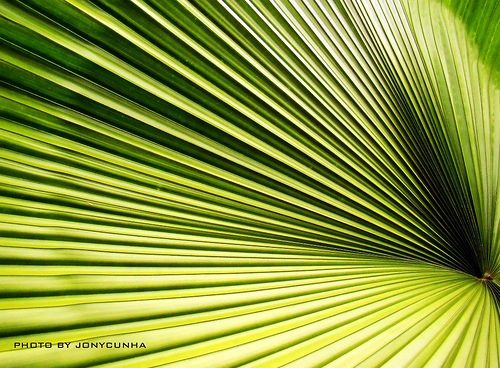
\includegraphics[width=0.95\textwidth]{/part01/convergence.jpg}
 \begin{center}
% {\large ``One door, one key\ldots''}\par
 Foto di Jonycunha\par
 \url{http://www.flickr.com/photos/jonycunha/4022906268/}\par
 Licenza: Creative Commons Attribution BY-SA\par
 \end{center}
\clearpage
\cleardoublepage 
% (c) 2014 Claudio.carboncinii - claudio.carboncini@gmail.com
% (c) 2014 Dimitrios Vrettos - d.vrettos@gmail.com
\chapter{Numeri reali}
\section{Dai numeri naturali ai numeri irrazionali}
Nel volume Algebra~1 abbiamo presentato i diversi insiemi numerici. Li riprendiamo brevemente per poi approfondire i numeri reali e le loro proprietà.

L'insieme dei \emph{numeri naturali} racchiude i numeri che utilizziamo per contare; si indica nel seguente modo:
\[\insN=\{0\text{, }1\text{, }2\text{, }3\text{, }4\text{, }5\text{, }6\text{, }7\text{, }8\text{, }9\text{, }10\text{, }11\text{, }\ldots\}\]

Su questi numeri sono definite le seguenti operazioni:
\begin{itemize*}
 \item \emph{addizione}: $n+m$~~è il numero che si ottiene partendo da $n$ e continuando a contare per altre $m$ unità;
 \item \emph{sottrazione}: $n-m$~~è il numero, se esiste ed è unico, che addizionato a $m$ dà come risultato $n$;
 \item \emph{moltiplicazione}: $n \cdot m$~~è il numero che si ottiene sommando $n$ volte $m$, o meglio sommando $n$ addendi tutti uguali a $m$;
 \item \emph{divisione}: $n:m$~~è il numero, se esiste ed è unico, che moltiplicato per $m$ dà come risultato $n$;
 \item \emph{potenza}: $n^{m}$~~è il numero che si ottiene moltiplicando $m$ fattori tutti uguali a $n$ con $m \ge 2$, ponendo $n^{1}=n$~~e~~$n^{0}=1$;
 \item \emph{radice}: $\sqrt[n]{m}$ con $n\ge 2$~~è il numero, se esiste ed è unico, che elevato a $n$ dà come risultato $m$.
\end{itemize*}

L'addizione, la moltiplicazione e la potenza sono definite su tutto l'insieme dei numeri naturali, cioè dati due numeri naturali qualsiasi, $n$ ed $m$, la somma $n+m$ e il loro prodotto $n \cdot m$ è sempre un numero naturale; la potenza $n^{m}$, escluso il caso $0^{0}$, è un numero naturale. Non sempre, invece, è possibile calcolare la differenza $n-m$, il quoziente $n:m$ o la radice $\sqrt[n]{m}$.

Tuttavia, dal punto di vista pratico-applicativo molto spesso si incontrano situazioni nelle quali occorre eseguire operazioni che non sempre è possibile eseguire con i soli numeri naturali. Iniziamo dall'operazione di sottrazione. Sappiamo che in tante situazioni di natura economica, ma non solo, deve essere possibile sottrarre un numero da uno più piccolo. Deve essere possibile, per esempio, comprare un'auto che costa \officialeuro~$12\,000$ anche quando in banca possediamo solo \officialeuro~$10\,000$. Deve quindi essere possibile eseguire una sottrazione del tipo $10\,000-12\,000$. Il risultato di questa operazione non va poi confuso con il risultato di $12\,000-10\,000$. Nel secondo caso, infatti, significa che sul nostro conto corrente abbiamo \officialeuro~$12\,000$ e dobbiamo spenderne $10\,000$, ci rimangono quindi \officialeuro~$2\,000$. Nel primo caso invece, possediamo \officialeuro~$10\,000$ e dobbiamo pagare
\officialeuro~$12\,000$, ci rimane quindi un debito di \officialeuro~$2\,000$. Per distinguere i due tipi di numeri mettiamo davanti al numero il segno ``$+$'' o il segno ``$-$''. Si genera così l'insieme dei \emph{numeri relativi}.
\[\insZ=\{\ldots\text{, }-3\text{, }-2\text{, }-1\text{, }0\text{, }+1\text{, }+2\text{, }+3\text{, }\ldots\}\]
Su questi numeri l'operazione di sottrazione è ovunque definita, in altre parole è sempre possibile eseguire la sottrazione tra qualunque numero di $\insZ$.

Non è invece sempre possibile eseguire le divisioni. Oltre ai casi $n:0$ e $0:0$, non è possibile, con i numeri interi, eseguire, ad esempio, la divisione $3:4$. Esistono però tante situazioni reali in cui una divisione di questo tipo deve poter essere eseguita. Per esempio è possibile dividere in parti uguali 3 uova in 4 persone, si può fare una frittata in una padella tonda e dividere la frittata in quattro parti uguali, a ciascuna persona toccano $\frac{3}{4}$ di uovo. Deve
essere possibile dividere in parti uguali 3 euro tra 4 persone. Dopo aver notato che a nessuno tocca 1 euro intero, si procede a cambiare le monete da 1 euro in monete da 1 decimo di euro, cioè da dieci centesimi, si cambiano quindi i 3 euro con 30 decimi di euro. Dividendo le 30 monete in 4 parti uguali risulta che ciascuno riceve 7 monetine e ne avanzano 2. Per dividere le 2 monete da un decimo si cambiano in monete da un centesimo, ottenendo 20 centesimi di euro. Si dividono allora le 20 monetine in 4 parti uguali, ciascuno avrà 5 centesimi di euro. In tutto a ciascuno toccano 75 centesimi di euro.

Per rappresentare il risultato di queste due operazioni di divisione abbiamo usato nel primo caso la notazione frazionaria $\frac{3}{4}$ e nel secondo caso la notazione decimale $\np{0,75}$. Le due scritture sono perfettamente equivalenti.

Per risolvere tutti i problemi di divisione i matematici hanno costruito l'insieme dei \emph{numeri razionali} che indichiamo nel seguente modo:
\[
\insQ=\left\{\frac{n}{m} \mid n\in \insZ\text{, }m\in \insN\text{, }m\neq
0\right\}=\left\{0\text{, }+1\text{, }-1\text{, }\frac{1}{2}\text{, }-\frac{1}{2}\text{, }+\frac{2}{3}\text{, }-\frac{1}{5}\text{, }-\frac{11}{17}\text{, }\frac{129}{\np{1725}}\text{, }\ldots\right\}
\]

Con questi numeri è possibile sempre eseguire l'addizione, la sottrazione, la moltiplicazione, la divisione (tranne con divisore 0) e l'elevazione a potenza.

Non sempre, invece, è possibile eseguire l'estrazione di radice. Per esempio, hai già conosciuto il numero $\sqrt{2}$, cioè il numero che elevato al quadrato dà 2; esso non è un numero razionale, cioè non può essere scritto né sotto forma di frazione né sotto forma di numero decimale finito o periodico. I numeri di questo tipo si dicono \emph{numeri irrazionali}.

%Abbiamo già affrontato questo problema nel volume di Algebra~1; per comodità del lettore riportiamo di seguito il ragionamento.
Riportiamo brevemente il ragionamento che ci permette di affermare che~$\sqrt{2}$ non è un numero razionale.

Fissiamo sulla retta orientata~$r$ l'unità di misura e disegniamo il quadrato $OABC$ di lato~1. Ci proponiamo di calcolare
la misura della lunghezza della sua diagonale~$OB$.

\begin{center}
 % (c) 2013 Claudio Carboncini - claudio.carboncini@gmail.com
\begin{tikzpicture}[x=10mm, y=10mm, font=\scriptsize]
  \draw [->] (0,0) -- (3,0) node [below] () {$r$};
  \draw (1,0) rectangle (2,1);
  \draw (1,0) -- (2,1);

  \coordinate[label=below:$O$] (O) at (1,0);
  \coordinate[label=below:$A$] (A) at (2,0);
  \coordinate[label=above:$C$] (C) at (1,1);
  \coordinate[label=above:$B$] (B) at (2,1);

  \begin{scope}[xshift=35mm]
    \draw [->] (0,0) -- (3,0) node [below] () {$r$};
    \draw (1,0) rectangle (2,1);
    \draw (1,0) -- (2,1);

    \coordinate[label=below:$O$] (O) at (1,0);
    \coordinate[label=below:$A$] (A) at (2,0);
    \coordinate[label=above:$C$] (C) at (1,1);
    \coordinate[label=above:$B$] (B) at (2,1);
    \coordinate[label=below:$K$] (K) at (2.414,0);

    \draw[dashed] (2.414,0) arc [start angle=0, end angle=65,radius=1.414cm,];

  \end{scope}
\end{tikzpicture}

\end{center}

Il triangolo~$OAB$ è retto in~$A$, quindi per il teorema di
Pitagora~$\overline{OB}^{2}=\overline{OA}^{2}+\overline{AB}^{2}$.
Sostituiamo le misure:~$\overline{OB}^{2}=1^2+1^2=2$. Per ottenere~$\overline{OB}$
dobbiamo estrarre la radice quadrata e quindi~$\overline{OB}=\sqrt{2}$.
Sappiamo che ``estrarre la radice quadrata'' di~2 significa trovare quel numero
che elevato al quadrato dà~2. Questo numero deve esistere, nel senso
che esiste sicuramente un punto sulla retta~$r$ che lo rappresenta, poiché lo si può costruire graficamente tracciando l'arco di
circonferenza di centro~$O$ e raggio~$\overline{OB}$, determinando così su $r$ il punto~$K$ estremo del segmento $OK$ con~$\overline{OK} = \overline{OB}$.

Dalla posizione del punto~$\sqrt{2}$ possiamo dire che~$1<\sqrt{2}<2$. Il
valore cercato evidentemente non è un numero intero. Può essere un
numero decimale finito? Compiliamo una tabella che contenga nella prima
riga i numeri con una sola cifra decimale compresi tra~1 e~2 e nella
seconda riga i rispettivi quadrati:

\begin{center}
\begin{tabular}{ccccccc}
\toprule
$x$ & $\np{1,1}$ & $\np{1,2}$ & $\np{1,3}$ & $\np{1,4}$ & $\np{1,5}$ & $\np{1,6}$\\
$x^{2}$ & $\np{1,21}$ & $\np{1,44}$ & $\np{1,69}$ & $\np{1,96}$ & $\np{2,25}$ & $\np{2,89}$\\
\bottomrule
\end{tabular}
\end{center}

Osserviamo che il numero~2 è compreso tra~$\np{1,4}^{2}$ e~$\np{1,5}^{2}$,
di conseguenza~$\np{1,4}<\sqrt{2}<\np{1,5}$, ma ancora
non possiamo precisare il suo valore, anche se abbiamo ristretto
l'intervallo in cui esso si trova. Diciamo che~$\np{1,4}$ è un valore approssimato per
difetto mentre~$\np{1,5}$
è un valore approssimato per eccesso; scrivendo~$\sqrt{2}=\np{1,4}$
oppure~$\sqrt{2}=\np{1,5}$ commettiamo un errore minore di~$1/10$.

Per migliorare l'approssimazione e tentare di ottenere~$\sqrt{2}$
come numero razionale costruiamo la tabella dei numeri
decimali con due cifre compresi tra~$\np{1,4}$ e~$\np{1,5}$:

\begin{center}
\begin{tabular}{ccccc}
\toprule
$x$ & $\np{1,41}$ & $\np{1,42}$ & $\np{1,43}$ & $\np{1,44}$\\
$x^{2}$ & $\np{1,9881}$ & $\np{2,0164}$ & $\np{2,0049}$ & $\np{2,0776}$\\
\bottomrule
\end{tabular}
\end{center}

Ora possiamo dire che~$\np{1,41}$ è un valore approssimato per difetto di~$\sqrt{2}$ mentre~$\np{1,42}$ è un valore approssimato
per eccesso, con un errore dell'ordine di~$1/100$. Abbiamo quindi migliorato
l'approssimazione e di conseguenza abbiamo ristretto l'intervallo in cui cade~$\sqrt{2}$, ma ancora non
abbiamo trovato un numero razionale che sia uguale a~$\sqrt{2}$.

Continuando con lo stesso procedimento costruiamo due classi di numeri razionali che approssimano una per difetto e
l'altra per eccesso il numero cercato, restringendo ogni volta l'ampiezza dell'intervallo in cui cade questo numero.
Il procedimento sembra non finire mai e le cifre decimali che troviamo non si ripetono periodicamente.

\begin{center}
 \begin{tabular}{lcll}
\toprule
Valore per difetto & Numero &Valore per eccesso & Ordine dell'errore\\
\midrule
$1$           & $\sqrt{2}$ & $2$           & 1\\
$\np{1,4}$    & $\sqrt{2}$ & $\np{1,5}$    & $10^{-1}$\\
$\np{1,41}$   & $\sqrt{2}$ & $\np{1,42}$   & $10^{-2}$\\
$\np{1,414}$  & $\sqrt{2}$ & $\np{1,415}$  & $10^{-3}$\\
$\np{1,4142}$ & $\sqrt{2}$ & $\np{1,4143}$ & $10^{-4}$\\
\ldots        & $\sqrt{2}$ & \ldots        & \ldots\\
\bottomrule
\end{tabular}
\end{center}

Per arrivare a concludere che~$\sqrt{2}$ non è un numero razionale,
possiamo ragionare nel seguente modo. Supponiamo per assurdo che~$\sqrt{2}$
sia un numero razionale e precisamente $\sqrt{2}=\frac{a}{b}$ con~$a$ e~$b$ primi tra loro. Se si eleva al quadrato $\sqrt{2}$ si ottiene $2=\frac{a^{2}}{b^{2}}$.
Elevare un numero al quadrato significa elevare al quadrato le
singole potenze dei fattori primi in cui esso si scompone. I fattori
primi di~$a^{2}$ e di~$b^{2}$ sono gli stessi di~$a$ e di~$b$ con
gli esponenti raddoppiati, quindi anche~$a^{2}$ e~$b^{2}$
sono primi tra loro e pertanto~$a^{2}$ non può essere il doppio di~$b^{2}$.
Quindi~$2\ne\frac{a^{2}}{b^{2}} \:\Rightarrow\: \sqrt{2}\ne\frac{a}{b}$.

Oltre a $\sqrt{2}$ vi sono altri infiniti numeri che non possono essere scritti come frazione. Per esempio, tutte le radici quadrate di numeri naturali che non sono quadrati perfetti e tutte le radici quadrate di frazioni che non sono il quadrato di alcuna frazione. Ma anche le radici cubiche del tipo $\sqrt[{3}]{2}$, $\sqrt[{5}]{7}$, \dots Un altro famoso numero irrazionale che si incontra nelle misure geometriche è il numero $\pi$, che corrisponde alla
misura della circonferenza di diametro $1$.
Questi numeri, insieme ad altri che conoscerete in seguito, costituiscono l'insieme $\insJ$ dei \emph{numeri irrazionali}.

L'unione degli insiemi $\insQ$ e $\insJ$ definisce l'insieme $\insR$ dei \emph{numeri reali}.

\vspazio\ovalbox{\risolvi \ref{ese:1.1}}

\section{I numeri reali}

In base a quanto abbiamo detto prima, essendo $\insR=\insQ \cup \insJ$, i numeri reali sono tutti quei numeri che si possono scrivere in forma decimale con un numero finito o infinito di cifre, non necessariamente periodiche.
Per esempio, la frazione $\frac{17}{16}$ è uguale al numero decimale finito~$\np{1,0625}$.
La frazione $\frac{16}{17}$ è uguale al numero decimale periodico $\np{0,}\overline{9411764705882352}$.

Il numero $\pi$ è invece un numero decimale con infinite cifre, non periodico. Riportiamo alcune cifre. %:\protect\\

3,141 592 653 589 793 238 462 643 383 279 502 884 197 169 399 375 105 820 974 944 592 307 816 406 286
208 998 628 034 825 342 117 067 982 148 086 513 282 306 647 093 844 609 550 582 231 725 359 408 128 481 117 450 284 102
701 938 521 105 559 644 622 948 954 930 381 964 428 810 975 665 933 446 128 475 648 233 786 783 165 271 201 909 145 648
566 923 460 348 \ldots % 610 454 326 648 213 393 607 260 \ldots
%$\pi=\np{3,141592653589793238462643383279502884197169399375105820974944592}$
%$307\,816\,406\,286\,208\,998\,628\,034\,825\,342\,117\,067\,982\,148\,086\,513\,282\,306\,647\,093\,844\,609\,550\,582\,231$
%$725\,359\,408\,128\,481\,117\,450\,284\,102\,701\,938\,521\,105\,559\,644\,622\,948\,954\,930\,381\,964\,428\,810\,975\,665$
%$933\,446\,128\,475\,648\,233\,786\,783\,165\,271\,201\,909\,145\,648\,566\,923\,460\,348\,610\,454\,326\,648\,213\,393\,607$
%$260\,\ldots$

Nonostante i numeri irrazionali siano stati scoperti dallo stesso Pitagora\footnote{filosofo, matematico, astronomo, scienziato e politico della Grecia antica (570 $\aC$ ca. - 495 $\aC$ ca.).} o dai suoi allievi nel $IV$~secolo~$\aC$, solo nel $XIX$~secolo Augustin-Louis Cauchy\footnote{matematico e ingegnere francese (1789 - 1857).} e Richard Dedekind\footnote{matematico tedesco (1831 - 1916).} sono giunti a una formulazione rigorosa dei numeri reali.

In effetti, assumere che i numeri reali sono tutti quelli che si possono scrivere in forma decimale finita o infinita, del tipo $r=n+\np{0,}abcd\ldots$, dove $r$ è il numero reale, $n$ è la sua parte intera e $\np{0,}abcd\ldots$ è quella decimale, comporta dei problemi. Per esempio, i numeri interi hanno una doppia rappresentazione: $1=\np{0,}\overline{9}$ come i numeri decimali finiti: $\np{1,225}=\np{1,224}\overline{9}$. Occorre quindi escludere almeno i numeri decimali con il~9 periodico. Oltre questo problema rimane la difficoltà di eseguire le operazioni tra numeri decimali illimitati. Gli algoritmi per addizionare, sottrarre e moltiplicare due numeri richiedono di cominciare dall'ultima cifra, cosa che non è possibile per i numeri decimali che non finiscono mai. Altro problema non semplice da gestire è il fatto che una definizione di
questo tipo è strettamente legata al sistema di numerazione a base 10 che noi utilizziamo.

Già nel volume Algebra~1, nel paragrafo sulle relazioni di equivalenza, abbiamo visto come i matematici hanno potuto costruire l'insieme $\insZ$ degli interi relativi a partire dall'insieme di coppie ordinate di $\insN \times \insN$ e l'insieme $\insQ$ dei razionali relativi a partire dall'insieme di coppie ordinate di $\insZ \times \insZ_{0}$.
La questione a questo punto è: possiamo costruire l'insieme dei numeri reali a partire dall'insieme dei numeri razionali $\insQ$? Per rappresentare il numero $\sqrt{2}$ abbiamo costruito un insieme, che indichiamo con $A$, di numeri razionali il cui quadrato è minore di $2$ e un insieme, che indichiamo con $B$, di numeri razionali il cui quadrato è maggiore di $2$. Sembra allora che il numero $\sqrt{2}$ divida l'insieme dei numeri razionali $\insQ$ in due parti: quella dei numeri razionali $a\in A$ cioè tali che $a^{2}<2$ e quella dei numeri razionali $b\in B$ cioè tali che $b^{2}>2$. La coppia di insiemi $(A;B)$ caratterizza il numero $\sqrt{2}$, possiamo anzi identificare $\sqrt{2}$ proprio con la coppia $(A;B)$.
È questa l'idea alla base del ragionamento di Richard Dedekind e del sezionamento degli insiemi.

\begin{definizione}
Si chiama \emph{sezione} o \emph{partizione} di un insieme $X$, una coppia di sottoinsiemi non vuoti $A$ e $B$ tali che:~$A \cap B=\emptyset$,~~$A \cup B=X$,~~$\forall a \in A$, $\forall b \in B$~~$a<b$.
\end{definizione}

\begin{exrig}
 \begin{esempio}
 Sezioni
 \begin{itemize}
 \item Consideriamo i due insiemi $A$ e $B$ così definiti: $A=\left\{x\in \insQ \mid x<3\right\}$,\ \ 
$B=\left\{x\in \insQ \mid x \ge 3\right\}$. Essi definiscono una sezione di $\insQ$, infatti
$A \cap B=\emptyset$,~~$A \cup B=\insQ$ e, per come sono stati definiti, ogni elemento di $A$ è minore di ogni elemento di $B$; inoltre possiamo osservare che $A$ non ammette massimo, non essendoci in esso un numero che sia maggiore di tutti gli altri, mentre $B$ ammette il minimo che è 3.
 \item Siano $A=\left\{x\in \insQ \mid x<-1\right\}$,~~$B=\left\{x \in \insQ \mid x>0\right\}$ la coppia $(A;B)$ non è una sezione di $\insQ$ perché pur essendo $A\cap B=\emptyset$ non è $A\cup B=\insQ$.
 \item Siano $A=\left\{x\in \insQ \mid x \le \frac{2}{7}\right\}$,~~$B=\left\{x \in \insQ \mid x \ge \frac{2}{7}\right\}$, anche in questo caso la coppia $(A;B)$ non è una sezione di $\insQ$ poiché $A\cap B=\left\{\frac{2}{7}\right\}$.
 \item Costruiamo gli insiemi $A$ e $B$ nel seguente modo: $A$ sia l'unione dei numeri razionali negativi e l'insieme dei numeri razionali positivi il cui quadrato è minore di 2 e in $B$ mettiamo tutti i razionali positivi il cui quadrato è maggiore di 2. $A=\insQ^{-} \cup \left\{x \in \insQ^{+} \mid x^{2}<2\right\}$, $B=\left\{x \in \insQ^{+} \mid x^{2}>2\right\}$. Si ha $A \cap B=\emptyset$,~~$A\cup B=\insQ$ poiché $\sqrt{2}\notin\insQ$, inoltre ogni elemento di $A$ è minore di ogni elemento di $B$. Dunque $(A;B)$ è una sezione di $\insQ$, ma $A$ non ha massimo e $B$ non ha minimo, in quanto abbiamo già dimostrato che non esiste un numero razionale che ha $2$ come quadrato. Questa sezione individua un buco nell'insieme $\insQ$.
 \end{itemize}
 \end{esempio}
\end{exrig}

Gli esempi visti ci permettono di affermare che una partizione $(A;B)$ può essere di tre tipi.
\begin{itemize*}
\item $A$ ammette massimo e $B$ non ammette minimo;
\item $A$ non ammette massimo e $B$ ammette minimo;
\item $A$ non ammette massimo e $B$ non ammette minimo.
\end{itemize*}

\begin{definizione}
Si chiama \emph{elemento separatore} di una partizione $(A;B)$ di un insieme $X$, il massimo di $A$ o il minimo di $B$, nel caso in cui almeno uno di questi elementi esista.
\end{definizione}

Nel primo esempio, poiché esiste il minimo di $B$, la partizione $(A;B)$ ammette un elemento separatore e identifica il numero razionale $3$.
Nel quarto esempio non esiste un numero razionale che fa da elemento separatore, la sezione $(A;B)$ identifica un numero irrazionale.

\begin{definizione}
L'insieme $\insR$ dei \emph{numeri reali} è l'insieme di tutte le partizioni di $\insQ$. Chiamiamo
\emph{numero razionale} le partizioni che ammettono elemento separatore e \emph{numero irrazionale} le sezioni che non ammettono elemento separatore.
\end{definizione}

Ogni numero reale è quindi individuato da due insiemi di numeri razionali: il primo contiene tutte le approssimazioni per difetto e l'altro tutte le approssimazioni per eccesso.

Ritornando all'esempio precedente, il numero $\sqrt{2}$ è individuato dalla sezione costituita dagli insiemi $A=\left\{x\in \insQ \mid x<0 \vee x^{2}<2\right\}$ e $B=\left\{x\in \insQ^{+} \mid x^{2}>2\right\}$.
Nell'insieme $A$ ci sono tutti i numeri razionali negativi oltre quelli che approssimano $\sqrt{2}$ per difetto: \[A=\{1\text{, }\np{1,4}\text{, }\np{1,41}\text{, }\np{1,414}\text{, }\np{1,4142}\text{, }\np{1,41421}\text{, }\np{1,414213}\text{, }\ldots\}.\]
Nell'insieme $B$ ci sono tutti i numeri razionali positivi che approssimano $\sqrt{2}$ per eccesso:
\[B=\{2\text{, }\np{1,5}\text{, }\np{1,42}\text{, }\np{1,415}\text{, }\np{1,4143}\text{, }\np{1,41422}\text{, }\np{1,414214}\text{, }\ldots\}.\]

Questa costruzione dell'insieme dei numeri reali $\insR$ a partire dall'insieme dei numeri razionali
$\insQ$ è puramente astratta e formale, non serve al calcolo, vuole solo concludere il cammino intrapreso per costruire tutti gli insiemi numerici a partire dall'insieme dei numeri naturali $\insN$.

Dal punto di vista teorico è possibile definire nell'insieme delle partizioni di $\insQ$, l'ordinamento e le operazioni. Dal punto di vista del calcolo useremo le approssimazioni.

\begin{definizione}
Un insieme $X$ si dice \emph{continuo} se ogni partizione $(A;B)$ di $X$ ammette un solo elemento separatore, cioè se esiste un unico elemento $\overline{x}\in X$ tale che $\forall a \in A$, $\forall b \in B$ si ha $a\leq \overline{x}\leq b$.
\end{definizione}

\begin{teorema}[di Dedekind]
Ogni sezione $(A;B)$ dell'insieme $\insR$ ammette uno e un solo elemento separatore.
\end{teorema}

Da questo teorema segue che un numero reale è definito come elemento separatore di una sezione $(A;B)$ di $\insR$.

\begin{postulato}[di continuità della retta]
Esiste una corrispondenza biunivoca tra l'insieme dei punti della retta geometrica e l'insieme $\insR$ dei numeri reali.
\end{postulato}

Da questo postulato segue la possibilità di definire sulla retta un sistema di coordinate: ad ogni punto corrisponde un numero reale (la sua \emph{ascissa}) e viceversa ad ogni numero reale è associato uno e un solo punto sulla retta; analogamente si ha nel piano dove il sistema di assi cartesiano permette di realizzare una corrispondenza biunivoca tra coppie di numeri reali (\emph{ascissa} e \emph{ordinata} del punto) e un punto del piano geometrico. Vedremo in seguito che la possibilità di associare numeri e punti si estende anche allo spazio tridimensionale e oltre.

\subsection{Confronto fra numeri reali}

Per confrontare due numeri reali, osserviamo prima di tutto i segni. Se i segni dei numeri sono
discordi, il numero negativo è minore del numero positivo. Se i segni dei numeri sono concordi si valuta la parte intera del numero: se sono positivi è più grande quello che ha la parte intera maggiore, viceversa se sono negativi è più grande quello che ha la parte intera minore. A parità di parte intera bisogna confrontare la parte decimale partendo dalle cifre più a sinistra finché non si trova la prima cifra decimale diversa: se i numeri sono positivi è maggiore quello che ha la cifra maggiore; se sono negativi è maggiore quello che ha la cifra minore.

\pagebreak
\begin{exrig}
 \begin{esempio}
 Confrontare i seguenti numeri reali
 \begin{itemize}
 \item $\sqrt{2}$~~e~~$\sqrt{3}$.
 
 $\sqrt{2}<\sqrt{3}$. Per verificarlo ci si può aiutare con la calcolatrice per calcolare le prime cifre decimali dei due numeri $\sqrt{2}=\np{1,4142}\ldots$, $\sqrt{3}=\np{1,7320}\ldots$; oppure ci si arriva osservando che il numero che elevato al quadrato dà 2 deve essere minore del numero che elevato al quadrato dà 3;
 \item $\sqrt{99}$~~e~~$10$.
 
 $\sqrt{99}<10$. Per verificarlo è sufficiente osservare che $\sqrt{100}=10$.
 \end{itemize}
 \end{esempio}
\end{exrig}
\ovalbox{\risolvii \ref{ese:1.2}, \ref{ese:1.3}, \ref{ese:1.4}, \ref{ese:1.5}, \ref{ese:1.6}}\vspazio

\section{Valore assoluto}

Si definisce \emph{valore assoluto} di un numero reale $a$, indicato con $\valass{a}$, il numero stesso se $a$ è positivo o nullo, il suo opposto se $a$ è negativo. Pertanto il risultato dell'operazione valore assoluto è sempre un numero positivo.

\[
|a|=
\begin{cases}
a & \text{ se }a\ge 0\\
-a & \text{ se }a<0
\end{cases}.
\]

Il numero $a$ si dice argomento del valore assoluto.

\[\valass{-3}=3;\qquad\qquad\qquad\valass{+5}=5;\qquad\qquad\qquad\valass{0}=0.\]

\subsection{Proprietà del valore assoluto}
\begin{itemize}
 \item $\valass{x+y}\le \valass{x}+\valass{y}$: (\emph{disuguaglianza triangolare}) il valore assoluto della somma di due numeri è minore o uguale della somma dei valori assoluti dei due numeri. Si ha l'uguaglianza solo quando i due numeri reali hanno lo stesso segno, oppure quando almeno uno dei due numeri è nullo.

 \item $\valass{x-y}\le \valass{x}+\valass{y}$: il valore assoluto della differenza di due numeri è minore o uguale della somma dei valori assoluti dei due numeri.

 \item $\valass{x\cdot y}=\valass{x}\cdot \valass{y}$: il valore assoluto del prodotto di due numeri
è uguale al prodotto dei valori assoluti dei due numeri.

 \item $\left |{\dfrac{x}{y}}\right|=\dfrac{\valass{x}}{\valass{y}}$: il valore assoluto del rapporto di due
numeri è uguale al rapporto dei valori assoluti dei due numeri.
\end{itemize}

Se l'argomento del valore assoluto è una funzione $f(x)$ si ha:
\[\valass{f(x)}=
\begin{cases}
f(x) & \text{ se }f(x)\ge 0\\
-f(x) & \text{ se }f(x)<0
\end{cases}.\]
\pagebreak
\begin{exrig}
 \begin{esempio}
 Valore assoluto di numeri reali
 \begin{itemize}
 \item $\valass{5+3}=\valass{5}+\valass{3}$ in entrambi i casi si ottiene $8$;
 \item $\valass{5+(-3)}=2$ mentre $\valass{5}+\valass{-3}=8$, pertanto $\valass{5+(-3)}<\valass{5}+\valass{-3}$.
 \end{itemize}
 \end{esempio}
\end{exrig}

Nelle espressioni contenenti valori assoluti con argomento letterale si deve cercare di eliminare il
valore assoluto.
%\pagebreak
\begin{exrig}
 \begin{esempio}
 Valore assoluto con argomento letterale
 \begin{itemize}
 \item $\left|{x^{2}}\right|=x^{2}$ infatti $x^{2}$ è una quantità sempre non negativa;
 \item $\left|{a^{2}+1}\right|=a^{2}+1$ infatti $a^{2}$ è sempre non negativo, quindi sarà sempre $a^2+1 \ge 1 > 0$;
 \item $\valass{x-1}=\begin{cases}
x-1 & \text{ se }x\ge 1\\
-x+1 & \text{ se }x<1
\end{cases}$ una funzione di questo tipo si dice \emph{definita per casi};
 \item $f(a)=\valass{a+1}-3a+1$ acquista due significati a seconda che l'argomento del valore assoluto sia positivo o meno. La sua espressione algebrica è:
\[
f(a)=\valass{a+1}-3a+1=
\begin{cases}
a+1-3a+1=-2a+2 & \text{ se }a+1\ge 0\:\Rightarrow\: a\ge-1\\
-(a+1)-3a+1=-4a & \text{ se }a+1< 0\:\Rightarrow\: a<-1
\end{cases}.
\]
 \end{itemize}
 \end{esempio}
\begin{esempio}
 $f(x)=\valass{x-5}+\valass{x+2}$.

 La presenza di due valori assoluti ci obbliga a studiare i casi generati dal segno dei singoli argomenti.
 Pertanto poiché l'argomento del primo valore assoluto è non negativo per $x\ge 5$ e l'argomento del secondo valore assoluto è non negativo
 per $x\ge -2$, possiamo porre la reciproca situazione nel seguente grafico:
\begin{center}
% (c) 2013 Claudio Carboncini - claudio.carboncini@gmail.com
\begin{tikzpicture}[font=\small,x=10mm, y=10mm]

\draw[->] (0,0) -- (8,0) node [below right] () {$r$};

\foreach \x in {2,5}{
\draw(\x,3pt)--(\x,-3pt);
\begin{scope}[dotted]
\draw (\x,0) -- (\x,-1.5);
\draw (0,-.5) -- (5,-.5);
\draw (0,-1) -- (2,-1);
\end{scope}}

\node[above]  at (5,0) {$5$};
\node[above]  at (2,0) {$-2$};
\node [circle,fill=gray!30](A) at (1,-1.4) {A};
\node [circle,fill=gray!30](B) at (3.5,-1.4) {B};
\node [circle,fill=gray!30](C) at (6.5,-1.4) {C};

\begin{scope}[blue,thick]
\draw (5,-.5) -- (8,-.5);
\draw (2,-1) -- (8,-1);


\draw[fill=blue] (5,-.5)circle (1.5pt);
\draw[fill=blue] (2,-1)circle (1.5pt);

\end{scope}

\end{tikzpicture}

\end{center}

\begin{enumerate}[label={(\Alph*)}]
 \item se $x<-2$ entrambi gli argomenti sono negativi, pertanto 
\[f(x)=\valass{x-5}+\valass{x+2}=-x+5-x-2=-2x+3.\]
Se $x=-2$ si ha $f(-2)=\valass{-2-5}+0=7$;
 \item se $-2<x<5$ il primo argomento è negativo e il secondo è positivo, pertanto 
\[f(x)=\valass{x-5}+\valass{x+2}=-x+5+x+2=7.\]
Se $x=5$ si ha $f(5)=0+\valass{5+2}=7$;
 \item se $x>5$ entrambi gli argomenti sono positivi, pertanto 
\[f(x)=\valass{x-5}+\valass{x+2}=x-5+x+2=2x-3.\]
\end{enumerate}
Possiamo allora sintetizzare in questo modo
\[
\valass{x-5}+\valass{x+2}=
\begin{cases}
-2x+3 & \text{ se }x<-2\\
7 & \text{ se }-2\le x<5\\
2x-3 & \text{ se }x\ge 5
\end{cases}.
\]
\end{esempio}
\end{exrig}
\ovalbox{\risolvii \ref{ese:1.7}, \ref{ese:1.8}, \ref{ese:1.9}, \ref{ese:1.10}}

\newpage

% (c)~2014 Claudio Carboncini - claudio.carboncini@gmail.com
% (c)~2014 Dimitrios Vrettos - d.vrettos@gmail.com
\section{Esercizi}
\subsection{Esercizi dei singoli paragrafi}
\subsubsection*{1.1 - Dai numeri naturali ai numeri irrazionali}

\begin{esercizio}
\label{ese:1.1}
Dimostra, con un ragionamento analogo a quello fatto per $\sqrt 2$, che $\sqrt 3$ non è razionale.
\end{esercizio}

\subsubsection*{1.2 - I numeri reali}


\begin{esercizio}
\label{ese:1.2}
Per ciascuno dei seguenti numeri reali scrivi una sequenza di sei numeri razionali che lo approssimano per difetto e sei numeri razionali che lo approssimano per eccesso. Esempio:
$\sqrt{3}$: $A=\{1$, $\np{1,7}$, $\np{1,73}$, $\np{1,732}$, $\np{1,7320}$, $\np{1,73205}\}$,$\quad B=\{2$, $\np{1,8}$, $\np{1,74}$, $\np{1,733}$, $\np{1,7321}$, $\np{1,73206}\}$.
\begin{enumeratea}
 \item$\sqrt{5}$:\, $A=\{\ldots\ldots\ldots\ldots\ldots\ldots\ldots\ldots\}$,$\quad B=\{\ldots\ldots\ldots\ldots\ldots\ldots\ldots\ldots\}$;
 \item$\dfrac{6}{7}$:\, $A=\{\ldots\ldots\ldots\ldots\ldots\ldots\ldots\ldots\}$,$\quad B=\{\ldots\ldots\ldots\ldots\ldots\ldots\ldots\ldots\}$;
 \item$\dfrac{1}{7}$:\, $A=\{\ldots\ldots\ldots\ldots\ldots\ldots\ldots\ldots\}$,$\quad B=\{\ldots\ldots\ldots\ldots\ldots\ldots\ldots\ldots\}$;
 \item$\sqrt{2}+\sqrt{3}$:\, $A=\{\ldots\ldots\ldots\ldots\ldots\ldots\ldots\ldots\}$,$\quad B=\{\ldots\ldots\ldots\ldots\ldots\ldots\ldots\ldots\}$;
 \item$\sqrt{2}\cdot\sqrt{3}$:\, $A=\{\ldots\ldots\ldots\ldots\ldots\ldots\ldots\ldots\}$,$\quad B=\{\ldots\ldots\ldots\ldots\ldots\ldots\ldots\ldots\}$.
 \end{enumeratea}
\end{esercizio}

\begin{esercizio}[\Ast]
\label{ese:1.3}
Determina per ciascuno dei seguenti numeri irrazionali i numeri interi tra i quali è compreso. Esempio: $5<\sqrt{30}<6$.
\begin{multicols}{3}
\begin{enumeratea}
 \item~$\sqrt{50}$;
 \item~$\sqrt{47}$;
 \item~$\sqrt{91}$;
 \item~$\sqrt{73}$;
 \item~$\sqrt{107}$;
 \item~$\sqrt{119}$;
 \item~$\sqrt{5}+\sqrt{3}$;
 \item~$2\sqrt{7}$;
 \item~$2+\sqrt{7}$;
 \item~$\sqrt{20}-\sqrt{10}$;
 \item~$\sqrt{\frac{7}{10}}$;
 \item~$7+\sqrt{\frac{1}{2}}$.
\end{enumeratea}
\end{multicols}
\end{esercizio}

\begin{esercizio}
\label{ese:1.4}
 Disponi in ordine crescente i seguenti numeri reali:
 \begin{enumeratea}
 \item $\sqrt{2}$,\quad $1$,\quad $\dfrac{2}{3}$,\quad $\np{2,0}\overline{13}$,\quad $\sqrt{5}$,\quad $\dfrac{3}{2}$,\quad $\np{0,75}$.
 \item $\pi$,\quad $\sqrt{3}$,\quad $\dfrac{11}{5}$,\quad $\np{0,}\overline{9}$,\quad $\sqrt{10}$,\quad $\np{3,1}\overline{4}$,\quad $\sqrt[3]{25}$.
 \end{enumeratea}
\end{esercizio}

\begin{esercizio}
\label{ese:1.5}
 Rappresenta con un diagramma di Eulero-Venn l'insieme dei numeri reali $\insR$, suddividilo nei seguenti sottoinsiemi: l'insieme dei numeri naturali $\insN$, l'insieme dei numeri interi relativi~$\insZ$, l'insieme dei numeri razionali $\insQ$, l'insieme $\insJ$ dei numeri irrazionali. Disponi in maniera opportuna i seguenti numeri: $\sqrt{3}$,\quad $\sqrt[3]{5}$,\quad$\pi$,\quad $\np{0,}\overline{3}$,\quad $\np{3,14}$,\quad $\frac{3}{2}$,\quad$-2$.
\end{esercizio}

%\newpage
\begin{esercizio}[\Ast]
\label{ese:1.6}
Indica il valore di verità delle seguenti affermazioni:
\begin{enumeratea}
\item un numero decimale finito è sempre un numero razionale;
\item un numero decimale illimitato è sempre un numero irrazionale;
\item un numero decimale periodico è un numero irrazionale;
\item la somma algebrica di due numeri razionali è sempre un numero razionale;
\item la somma algebrica di due numeri irrazionali è sempre un numero irrazionale;
\item il prodotto di due numeri razionali è sempre un numero razionale;
\item il prodotto di due numeri irrazionali è sempre un numero irrazionale.
\end{enumeratea}
\end{esercizio}

\subsubsection*{1.3 - Valore assoluto}
\begin{esercizio}[\Ast]
\label{ese:1.7}
 Calcola il valore assoluto dei seguenti numeri:
\begin{multicols}{3}
 \begin{enumeratea}
 \item~$\valass{-5}$
 \item~$\valass{+2}$
 \item~$\valass{-1}$
 \item~$\valass{0}$
 \item~$\valass{-10}$
 \item~$\valass{3-5\cdot(2)}$
 \item~$\valass{-3+5}$
 \item~$\left|{(-1)^3}\right|$
 \item~$\valass{-1-2-3}$
% \item~$\valass{3(-2)-5}$
 \end{enumeratea}
 \end{multicols}
\end{esercizio}

\begin{esercizio}
\label{ese:1.8}
Dati due numeri reali $x$ ed $y$ entrambi non nulli e di segno opposto, verifica le seguenti relazioni con gli esempi numerici riportati sotto.
Quali delle relazioni sono vere in alcuni casi e false in altri, quali sono sempre vere, quali sono sempre false?
\begin{center}
 \begin{tabular}{lcccc}
\toprule
Relazione & $x=-3$, $y=5$&$x=-2$, $y=2$ &$x=-10$, $y=1$&$x=1$, $y=-5$\\
\midrule
$\valass{x}<\valass{y}$& \boxV\qquad\boxF& \boxV\qquad\boxF&\boxV\qquad\boxF&\boxV\qquad\boxF\\
$\valass{x}=\valass{y}$& \boxV\qquad\boxF& \boxV\qquad\boxF&\boxV\qquad\boxF&\boxV\qquad\boxF\\
$\valass{x}<y$& \boxV\qquad\boxF& \boxV\qquad\boxF&\boxV\qquad\boxF&\boxV\qquad\boxF\\
$\valass{x+y}<\valass{x}+\valass{y}$& \boxV\qquad\boxF& \boxV\qquad\boxF&\boxV\qquad\boxF&\boxV\qquad\boxF\\
$\valass{x-y}=\valass{x}-\valass{y}$& \boxV\qquad\boxF& \boxV\qquad\boxF&\boxV\qquad\boxF&\boxV\qquad\boxF\\
$\left|{\valass{x}-\valass{y}}\right|=\valass{x-y}$& \boxV\qquad\boxF& \boxV\qquad\boxF&\boxV\qquad\boxF&\boxV\qquad\boxF\\
\bottomrule
\end{tabular}
\end{center}
\end{esercizio}

\begin{esercizio}[\Ast]
\label{ese:1.9}
 Elimina il valore assoluto sostituendo le espressioni con una funzione definita per casi:
 \begin{multicols}{2}
 \begin{enumeratea}
 \item~$f(x)=\left|x+1\right|$;
 \item~$f(x)=\left|x-1\right|$;
 \item~$f(x)=\left|x^2+1\right|$;
 \item~$f(x)=\left|(x+1)^2\right|$;
 \item~$f(x)=\left|x^2-1\right|$;
 \item~$f(x)=\left|x^3-1\right|$;
 \item~$f(x)=\left|x^2-6x+8\right|$;
 \item~$f(x)=\left|x^2+5x+4\right|$.
 \end{enumeratea}
 \end{multicols}
\end{esercizio}

\begin{esercizio}[\Ast]
\label{ese:1.10}
 Elimina il segno di valore assoluto dalle seguenti espressioni sostituendole con una funzione definita per casi:
 \begin{multicols}{2}
 \begin{enumeratea}
 \item~$f(x)=\dfrac{\left|x+1\right|}{\left|x+2\right|}$;
 \item~$f(x)=\left|\dfrac{x+1}{x-1}\right|$;
 \item~$f(x)=\left|x+1\right|+\left|x-2\right|$;
 \item~$f(x)=\left|x+2\right|+\left|x-2\right|$;
 \item~$f(x)=\left|x-2\right|+\left|x-3\right|$;
 \item~$f(x)=\left|x+1\right|\cdot \left|x+2\right|$;
 \item~$f(x)=\left|\dfrac{x+1} 4\right|+\left|\dfrac{x+2}{x+1}\right|$;
 \item~$f(x)=\left|\dfrac{x+1}{x+2}\right|+\left|\dfrac{x+2}{x+1}\right|$.
 \end{enumeratea}
 \end{multicols}
\end{esercizio}

\subsection{Risposte}

\paragraph{1.3.}
a)~$7<\sqrt{50}<8$,\quad g)~$3<\sqrt{5}+\sqrt{3}<4$,\quad h)~$5<2\sqrt{7}<6$,\quad i)~$4<2+\sqrt{7}<5$.

\paragraph{1.6.}
a)~V,\quad b)~F,\quad c)~F,\quad d)~V,\quad e)~V,\quad f)~F,\quad g)~F.

\paragraph{1.7.}
a)~5,\quad b)~0,\quad c)~2,\quad d)~2,\quad e)~10,\quad f)~1,\quad g)~1,\quad h)~7,\quad i)~6.

\paragraph{1.9.}
a)~${x+1}\text{ se }x\ge-1\text{; }-x-1\text{ se }x<-1$,\quad b)~${x-1}\text{ se }x\ge 1\text{; }1-x\text{ se }x<1$.

\paragraph{1.10.}
a)~$\frac{x+1}{x+2}\text{ se }x<-2 \vee x>-1\text{; }-\frac{x+1}{x+2}\text{ se }-2<x<-1\text{; }0\text{ se }x=-1\text{; senza significato se }x~=~-2$.


\cleardoublepage 
% (c)~2012 Dimitrios Vrettos - d.vrettos@gmail.com
% (c)~2014 Claudio.carboncinii - claudio.carboncini@gmail.com
\chapter{Radicali}
\section{Radici}
\subsection{Radici quadrate}
Ricordiamo che il quadrato di un numero reale $a$ è il numero che si ottiene moltiplicando $a$ per se stesso. Il quadrato di un numero è sempre un numero non negativo; numeri opposti hanno lo stesso quadrato: $(+3)^2=9$,~~$(-2)^2=+4$,~~$(-5)^2=(+5)^2=+25$.

L'operazione inversa dell'elevamento al quadrato si chiama \emph{radice quadrata}. La radice quadrata di un numero reale $a$ è allora quel numero che elevato al quadrato, cioè, che moltiplicato per se stesso, dà il numero $a$.

\osservazione Non esiste la radice quadrata di un numero negativo, poiché non esiste un numero che elevato al quadrato possa dare come risultato un numero negativo.

\begin{definizione}
Si dice \emph{radice quadrata} di un numero reale $a$ positivo o nullo quel numero reale positivo o nullo che elevato al quadrato dà come risultato $a$.
In simboli~$\sqrt{a}=b \Leftrightarrow b^2=a$ dove $a$, $b\in \insR^{+}\cup \{0\}$.
\end{definizione}

Il simbolo $\sqrt{\phantom{5}}$ è il simbolo della radice quadrata; il numero $a$ è detto \emph{radicando}, il numero $b$ è detto \emph{radice quadrata} di $a$.

Dalla definizione $\sqrt{a^2}=a$ con $a\ge 0$, quindi $\sqrt{81}=9$ perché $9^2=81$; $\sqrt{\frac{9}{64}}=\frac{3}{8}$ perché~$\left(\frac{3}{8}\right)^2=\frac{9}{64}$.

\osservazione $\sqrt{81}=\sqrt{(-9)^2}$, ma $\sqrt{(-9)^2}\neq-9$ perché nella definizione di radice quadrata abbiamo imposto che il risultato dell'operazione di radice quadrata sia sempre un numero positivo o nullo.
Questa osservazione ci induce a porre molta attenzione quando il radicando è un'espressione letterale: in questo caso $\sqrt{a^2}=a$ non è del tutto corretto poiché $a$ può assumere sia valori positivi sia valori negativi. Scriveremo correttamente~$\sqrt{a^2}=\valass{a}$.

\begin{exrig}
\begin{esempio}
Radici quadrate
 \begin{multicols}{2}
\begin{itemize}
\item $\sqrt{4}=2\:$ infatti $2^2=4$;
\item $\sqrt{\dfrac{9}{16}}=\dfrac{3}{4}\:$ infatti $\left(\dfrac{3}{4}\right)^2=\dfrac{9}{16}$;
\item $\sqrt{\np{0,01}}=\np{0,1}\:$ infatti $\np{0,1}^2=\np{0,01}$;
\item $\sqrt{1}=1\:$ infatti $1^2=1$;
\item $\sqrt{0}=0\:$ infatti $0^2=0$;
\item $\sqrt{-16}\:$ non esiste poiché il radicando è negativo;
\item $\sqrt{11}\:$ esiste ma non è un numero intero né razionale, è un numero irrazionale;
\item $\sqrt{x^2}=\left|x\right|\:$ dobbiamo mettere il valore assoluto al risultato perché non conoscendo il segno di $x$ dobbiamo imporre che il risultato sia sicuramente positivo;
\item $\sqrt{a^2-4a+4}=\sqrt{(a-2)^2}=\left|a-2\right|\:$ dobbiamo mettere il valore assoluto perché $a-2$ potrebbe essere negativo;
\item $\sqrt{9(x+1)^2}=3\left|x+1\right|\:$ dobbiamo mettere il valore assoluto perché $x+1$ potrebbe essere negativo.
\end{itemize}
\end{multicols}
\end{esempio}
\end{exrig}

\subsection{Radici cubiche}
\begin{definizione}
 Si dice \emph{radice cubica} di un numero reale $a$ quel numero che, elevato al cubo, dà come risultato $a$. In simboli $\sqrt[3]{a}=b \Leftrightarrow b^3=a$ dove $a$, $b\in \insR$.
\end{definizione}

Puoi notare che la radice cubica di un numero reale esiste sempre sia per i numeri positivi o nulli, sia per i numeri negativi.

\begin{exrig}
\begin{esempio}
Radici cubiche
 \begin{multicols}{2}
 \begin{itemize}
\item $\sqrt[3]{-8}=-2\:$ infatti $\left(-2\right)^3=-8$;
\item $\sqrt[3]{125}=5\:$ infatti $5^3=125$;
\item $\sqrt[3]{1}=1\:$ infatti $1^3=1$;
\item $\sqrt[3]{0}=0\:$ infatti $0^3=0$;
\item $\sqrt[3]{\dfrac{1}{8}}=\dfrac{1}{2}\:$ infatti $\left(\dfrac{1}{2}\right)^3=\dfrac{1}{8}$;
\item $\sqrt[3]{\np{0,125}}=\np{0,5}\:$ infatti $(\np{0,5})^3=\np{0,125}$;
\item $\sqrt[3]{\np{-64}}=-4\:$ infatti $\left(-4\right)^3=\np{-64}$;
\item $\sqrt[3]{x^3}=x\:$ (per le radici cubiche non si deve mettere il valore assoluto);
\item $\sqrt[3]{x^3+3x^2+3x+1}=\sqrt[3]{(x+1)^3}=x+1\:$ (non si deve mettere il valore assoluto).
\end{itemize}
\end{multicols}
\end{esempio}
\end{exrig}

Osserva che la radice cubica di un numero mantiene sempre lo stesso segno del numero in quanto il cubo di un numero reale conserva sempre il segno della base.

\subsection{Radici n-esime}

Oltre alle radici quadrate e cubiche si possono considerare radici di indice qualsiasi. Si parla in generale di radice $n$-esima per indicare una radice con un qualsiasi indice $n$.

\begin{definizione}
Si dice \emph{radice $n$-esima} di un numero reale a quel numero $b$ che elevato ad $n$ dà come risultato $a$.
In simboli~$\sqrt[n]{a}=b \Leftrightarrow b^n=a$ con $n\in \insN$, $n\ge 2$.

Non si definisce la radice di indice $0$ e la scrittura $\sqrt[0]{a}$ è priva di significato. Alla scrittura~$\sqrt[1]{a}$ si dà il valore $a$.
\end{definizione}

Quando si tratta con le radici $n$-esime di un numero reale, bisogna fare attenzione se l'indice della radice è pari o dispari. Si presentano infatti i seguenti casi:
\begin{itemize}
 \item se l'indice $n$ è \emph{dispari} $\sqrt[n]{a}$ è definita per qualsiasi valore di $a\in \insR$, inoltre è negativa se~$a<0$, positiva se $a>0$ e nulla se $a=0$;
 \item se l'indice $n$ è \emph{pari} $\sqrt[n]{a}$ è definita solo per i valori di $a\geq 0$ e si ha che $\sqrt[n]{a}\ge 0$.
\end{itemize}
%\newpage
\pagebreak
\begin{exrig}
\begin{esempio}
Radici $n$-esime
\begin{multicols}{2}
 \begin{itemize}
 \item $\sqrt[4]{16}=2\:$ infatti $2^4=16$;
 \item $\sqrt[4]{-16}\:$ non esiste, poiché $(-2)^4=+16$;
 \item $\sqrt[5]{32}=2\:$ infatti $2^5=32$;
 \item $\sqrt[5]{-32}=-2\:$ infatti $(-2)^5=-32$;
 \item $\sqrt[4]{1}=1\:$ infatti $1^4=1$;
 \item $\sqrt[n]{0}=0$;
 \item $\sqrt[5]{-1}=-1\:$ infatti $(-1)^5=-1$;
 \item $\sqrt[4]{x^4}=\left|x\right|\:$ va messo il valore assoluto perché l'indice della radice è pari;
 \item $\sqrt[5]{x^5}=x\:$ non va messo il valore assoluto perché l'indice della radice è dispari.
\end{itemize}
\end{multicols}
\end{esempio}
\end{exrig}

\ovalbox{\risolvii \ref{ese:2.1}, \ref{ese:2.2}, \ref{ese:2.3}, \ref{ese:2.4}, \ref{ese:2.5}, \ref{ese:2.6}, \ref{ese:2.7}, \ref{ese:2.8}, \ref{ese:2.9}, \ref{ese:2.10}}

\section{Condizioni di esistenza}

Quando il radicando è un'espressione letterale dobbiamo fare molta attenzione a operare su di esso.
Le \emph{condizioni di esistenza}, in breve si può scrivere $\CE$, di un radicale con radicando letterale, sono le condizioni cui devono soddisfare le variabili che compaiono nel radicando affinché la radice abbia significato.

Supponiamo di avere $\sqrt[n]{A(x)}$ con $A(x)$ espressione nella variabile $x$, dobbiamo distinguere i seguenti casi:
\begin{itemize*}
\item se $n$ è \emph{pari} la radice esiste per tutti i valori di $x$ che rendono non negativo il radicando, cioè $\CE\: A(x)\ge 0$;
\item se $n$ è \emph{dispari} la radice esiste per qualsiasi valore della variabile $x$, purché esista il radicando stesso.
\end{itemize*}

\begin{exrig}
\begin{esempio}
Condizioni di esistenza
 \begin{itemize}
 \item $\sqrt{x}$:\quad $\CE\: x\ge 0$;
 \item $\sqrt[3]{x}$:\quad $\CE\: \forall x\in \insR$;
 \item $\sqrt{-x}$:\quad $\CE\: x\le 0$;
 \item $\sqrt[3]{-x}$:\quad $\CE\: \forall x\in \insR$;
 \item $\sqrt{x-1}$:\quad $\CE\: x-1\ge 0 \:\Rightarrow\: x\ge 1$;
 \item $\sqrt{a^2+1}$:\quad $\CE\: \forall a\in \insR$, infatti $a^2$ è sempre positivo pertanto $a^2+1>0$, $\forall a\in \insR$;
 \item $\sqrt[3]{\frac{1}{x+1}}$:\quad la radice cubica è definita per valori sia positivi sia negativi del radicando, tuttavia bisogna comunque porre la condizione che il denominatore della frazione non sia nullo, quindi $\CE\: x+1\neq 0 \:\Rightarrow\: x\neq -1$;
 \item $\sqrt[4]{xy}$:\quad $\CE\: xy\ge 0$;
 \item $\sqrt[5]{a^2(a-3)}$: poiché la radice ha indice dispari non occorre porre alcuna condizione di esistenza.
\end{itemize}
\end{esempio}

\begin{esempio}
 Determina le condizioni di esistenza della seguente espressione: $\sqrt{x}+\sqrt{x+1}$.

$\CE$: $\sqrt{x}$ esiste per $x\ge 0$, $\sqrt{x+1}$ esiste per $x+1\ge 0\:\Rightarrow\: x\ge -1$, quindi per individuare le condizioni di esistenza dell'espressione occorre risolvere il sistema $\left\{\begin{array}{l} x\ge0\\ x\ge-1\end{array}\right.$.
\begin{center}
 % (c) 2013 Claudio Carboncini - claudio.carboncini@gmail.com
\begin{tikzpicture}[font=\small,x=10mm, y=10mm]

\draw[->] (0,0) -- (8,0) node [below right] () {$r$};

\foreach \x in {2,5}{
\draw(\x,3pt)--(\x,-3pt);
\begin{scope}[dotted]
\draw (\x,0) -- (\x,-1.5);
\draw (0,-.5) -- (2,-.5);
\draw (0,-1) -- (5,-1);
\end{scope}}

\node[above]  at (2,0) {$-1$};
\node[above]  at (5,0) {$0$};
\pattern[pattern= north east lines, pattern color=red] (5,-1) rectangle (8,-1.5);

\node[below] () at (6.5,-1.5) {$\IS$};

\begin{scope}[blue,thick]
\draw (2,-.5) -- (8,-.5);
\draw (5,-1) -- (8,-1);

\draw[fill=blue] (2,-.5)circle (1.5pt);
\draw[fill=blue] (5,-1)circle (1.5pt);

\end{scope}

\end{tikzpicture}

\end{center}

In definitiva $\CE\: x\ge 0$.
\end{esempio}

\begin{esempio}
 Determina le condizioni di esistenza della radice $\sqrt[4]{\dfrac{x-1}{x+1}}$.

$\CE\: \dfrac{x-1}{x+1}\ge 0$. Il segno della frazione $F$ si ottiene dalla combinazione del segno del numeratore $N$ e del denominatore $D$:
\begin{center}
 % (c) 2013 Claudio Carboncini - claudio.carboncini@gmail.com
\begin{tikzpicture}[font=\small,x=10mm, y=10mm]

\draw[->] (0,0) -- (8,0) node [below right] () {$r$};

\foreach \x in {2,5}{
\draw(\x,3pt)--(\x,-3pt);
\begin{scope}[dotted]
\draw (\x,0) -- (\x,-1.5);
\draw (0,-.5) -- (5,-.5);
\draw (0,-1) -- (2,-1);
\end{scope}}

\node[above]  at (2,0) {$-1$};
\node[above]  at (5,0) {$1$};

\begin{scope}[blue,thick]
\draw (5,-.5) -- (8,-.5);
\draw (2,-1) -- (8,-1);

\draw[fill=blue] (5,-.5)circle (1.5pt);
\draw[fill=white] (2,-1)circle (1.5pt);
\end{scope}

\foreach \x in {-1.5}{
\node  at (\x,-.25) {segno di $N$:};
\node  at (\x,-.75) {segno di $D$:};
\node  at (\x,-1.25) {segno di $F$:};
}
\foreach \z in {1,3.5}{
\node  at (\z,-.25) {$-$};
}
\foreach \zi in {3.5, 6.5}{
\node  at (\zi,-.75) {$+$};
}

\node  at (6.5,-.25) {$+$};
\node  at (1,-.75) {$-$};

\begin{scope}[red]
\foreach \zii in {1, 6.5}{
\node  at (\zii,-1.25) {$+$};
}
\node  at (3.5,-1.25) {$-$};
\end{scope}
\end{tikzpicture}

\end{center}
Pertanto $\CE\: x<-1\vee x\ge 1$.
\end{esempio}
\end{exrig}

\vspazio\ovalbox{\risolvii \ref{ese:2.11}, \ref{ese:2.12}, \ref{ese:2.13}, \ref{ese:2.14}, \ref{ese:2.15}, \ref{ese:2.16}, \ref{ese:2.17}}

\section{Potenze ad esponente razionale}

In questo paragrafo ci proponiamo di scrivere la radice $n$-esima di un numero reale $a\geq0$ sotto forma di potenza di $a$, vogliamo cioè che sia:
$\sqrt[n]{a}=a^x$.

\paragraph {Caso con esponente positivo}
Elevando ambo i membri dell'uguaglianza alla potenza n otteniamo: $\left(\sqrt[n]a\right)^n=\left(a^x\right)^n$ da cui si ottiene $a=a^{n\cdot x}$.
Trattandosi di due potenze con base~$a{\geq}0$, l'uguaglianza è resa possibile solo se sono uguali gli esponenti. In altre parole, deve essere: $1=n\cdot x \Rightarrow x=\dfrac 1 n$, quindi: $\sqrt[n]a=a^{\frac 1 n}$.

Vediamo ora di generalizzare la formula. Sia $m$ un numero intero positivo, possiamo scrivere $a^{\frac m n}=\left(a^{\frac 1 n}\right)^m$ e quindi $a^{\frac m n}=\left(\sqrt[n]a\right)^m$.
\begin{exrig}
\begin{esempio}
 Calcola le seguenti potenze a esponente razionale positivo.
 \begin{itemize*}
 \item~$27^{\frac 2 3}$: si ha che $27^{\frac 2 3}=\left(\sqrt[3]{27}\right)^2=3^2=9$;
 \item~$25^{\frac 3 2}$: si ha che $25^{\frac 3 2}=\left(\sqrt[2]{25}\right)^3=5^3=125$.
\end{itemize*}
\end{esempio}
\end{exrig}

\paragraph{Caso con esponente negativo}
Per definire la potenza ad esponente razionale negativo è necessario imporre la restrizione $a \neq 0$, infatti risulta:
$a^{-\frac{m}{n}}=\dfrac{1}{a^{\frac{m}{n}}}=\left(\dfrac{1}{a}\right)^{\frac{m}{n}}$

\begin{exrig}
\begin{esempio}
 Calcola le seguenti potenze a esponente razionale negativo.
 \begin{itemize*}
 \item $27^{-\frac{2}{3}}=\dfrac 1{\left(\sqrt[3]{27}\right)^2}=\dfrac 1{3^2}=\dfrac 1 9$;
 \item $125^{-\frac 2 3}=\sqrt[3]{125^{-2}}=\sqrt[3]{(5^3)^{-2}}=\sqrt[3]{(5^{-2})^3}=5^{-2}=\dfrac 1{25}$;
 \item $\left(\dfrac 1 8\right)^{-\frac 3 2}=\sqrt{\left(\dfrac 1 8\right)^{-3}}=\sqrt{8^3}=\sqrt{(2^3)^3}=\sqrt{2^9}$;
 \item $\left(\dfrac 1{49}\right)^{-\frac 1 2}=(49)^{\frac 1 2}=\sqrt{49}=7$.
\end{itemize*}
\end{esempio}
\end{exrig}

In generale si dà la seguente
\begin{definizione}
Si dice \emph{potenza a esponente razionale} $\dfrac{m}{n}$ di un numero reale positivo $a$ l'espressione:
 $a^{\frac{m}{n}}=\sqrt[n]{a^m}=\left(\sqrt[n]{a}\right)^m$ con $\dfrac{m}{n}\in \insQ$.
\end{definizione}

Perché abbiamo dovuto imporre la condizione che $a$ sia un numero positivo?
Partiamo dall'espressione $a^{\frac{1}{n}}$ con $n\in \insN-\{0\}$, se $n$ è dispari la potenza $a^{\frac{1}{n}}$ è sempre definita per ogni valore della base $a$, mentre se è pari $a^{\frac{1}{n}}$ è definita solo per $a\geq 0$.

Nel caso generale, quindi, $a^{\frac{m}{n}}$ con $\dfrac{m}{n}\in \insQ$ la formula $a^{\frac{m}{n}}=\left(\sqrt[n]{a}\right)^m$ è falsa se $a<0$.

Consideriamo il seguente esempio:
 $(-2)^{\frac 6 6}=\left[(-2)^{\frac 1 6}\right]^6=\left(\sqrt[6]{-2}\right)^6$ non è definita nei numeri reali perché non esiste la radice sesta di un numero negativo.
Tuttavia possiamo anche scrivere 
\[(-2)^{\frac 6 6}=\left[(-2)^6\right]^{\frac 1 6}=(64)^{\frac 1 6}=\sqrt[6]{64}=2.\]
Arriviamo pertanto a due risultati differenti.

Per estendere la definizione al caso di basi negative sarebbe necessario stabilire un ordine di priorità delle operazioni ma ciò andrebbe contro la proprietà commutativa del prodotto degli esponenti di una potenza di potenza.

\vspazio\ovalbox{\risolvii \ref{ese:2.18}, \ref{ese:2.19}, \ref{ese:2.20}, \ref{ese:2.21}, \ref{ese:2.22}}

\section{Semplificazione di radici}

\begin{proposizione}
Il valore di una radice in $\insR^+\cup \{0\}$ non cambia se moltiplichiamo l'indice della radice e l'esponente del radicando per uno stesso numero intero positivo. In simboli $\sqrt[n]{a^m}=\sqrt[nt]{a^{mt}}$ con $a\ge 0$ e $m$, $n$, $t\in \insN-\{0\}$.
\end{proposizione}
\pagebreak
\begin{exrig}
 \begin{esempio}
 Radici equivalenti.
 \begin{itemize}
 \item $\sqrt{2}=\sqrt[4]{2^2}$: abbiamo moltiplicato per $2$ indice della radice ed esponente del radicando;
 \item $\sqrt[3]{a}=\sqrt[9]{a^3}$: abbiamo moltiplicato per $3$ indice della radice ed esponente del radicando.
\end{itemize}
 \end{esempio}
\end{exrig}

\begin{proposizione}
Il valore di una radice in $\insR^{+}\cup \{0\}$ non cambia se dividiamo l'indice della radice e l'esponente del radicando per un loro divisore comune. In simboli $\sqrt[nt]{a^{mt}}=\sqrt[n]{a^m}$ con $a\ge 0$ e $m$, $n$, $t\in \insN-\{0\}$.
\end{proposizione}

\begin{exrig}
 \begin{esempio}
Semplificazione di radici
\begin{itemize}
 \item $\sqrt[4]{2^2}=\sqrt 2$: abbiamo semplificato per $2$ indice della radice ed esponente del radicando;
 \item $\sqrt[10]{3^{15}}=\sqrt{3^3}$: abbiamo semplificato per $5$;
 \item $\sqrt[7]{3^9}$: non è riducibile perché indice della radice ed esponente non hanno divisori comuni;
 \item $\sqrt[8]{2^6}=2^{\frac 6 8}$: semplificando la frazione dell'esponente otteniamo $2^{\frac 3 4}=\sqrt[4]{2^3}$;
 \item $\sqrt[6]{\left(\dfrac 1 5\right)^{-9}}=\sqrt[6]{5^9}=\sqrt[2]{5^3}$;
 \item $\sqrt[4]{(-3)^2}=\sqrt[4]{3^2}=\sqrt 3$;
 \item $\sqrt{10^{-4}}$: semplificando per $2$ indice della radice ed esponente del radicando si ottiene~$10^{-2}=\dfrac 1{100}$;
 \item $\sqrt{30\cdot 27\cdot 10}$: scomponendo in fattori primi otteniamo \[\sqrt{30\cdot 27\cdot 10}=\sqrt{2\cdot 3\cdot 5\cdot 3^3\cdot 2\cdot 5}=\sqrt{2^2\cdot 3^4\cdot 5^2}.\] Osserviamo che tutti gli esponenti del radicando e l'indice della radice hanno in comune il divisore 2, quindi $\sqrt{2^2\cdot 3^4\cdot 5^2}=2\cdot 3^2\cdot 5=90.$
\end{itemize}
\end{esempio}
\end{exrig}

Se il radicando è un'espressione letterale, quindi è possibile che sia positiva che negativa, dobbiamo scrivere
\[
\sqrt[nt]{a^{mt}}=
\begin{cases}
\sqrt[n]{a^m} & \text{ se }t\text{ è dispari}\\
\sqrt[n]{\left|a^m\right|} & \text{ se }t\text{ è pari}
\end{cases}.
\]

\begin{exrig}
 \begin{esempio}
Semplificazione di radici con espressione letterale come radicando.
\begin{itemize}
\item $\sqrt{4x^4y^2a^6}=\sqrt{2^2x^4y^2a^6}=2x^2\left|ya^3\right|$: abbiamo semplificato per $2$ sia l'indice della radice che l'esponente del radicando;
\item $\sqrt[12]{a^2+2a+1}=\sqrt[12]{(a+1)^2}=\sqrt[6]{\left|a+1\right|}$: dopo aver riconosciuto che il radicando è il quadrato del binomio, abbiamo semplificato per $2$ indice ed esponente;
\item $\sqrt{x^2y^2}=\valass{xy}$;
\item $\sqrt{x^2+2xy+y^2}=\sqrt{(x+y)^2}=\valass{x+y}$;
\item $\sqrt{x^2+y^2}$ non è semplificabile perché il radicando non può essere espresso sotto forma di potenza;
\item $\sqrt[6]{(x-1)^2}=\sqrt[3]{\valass{x-1}}$;
\end{itemize}
 \end{esempio}
\end{exrig}

La proprietà invariantiva si può applicare per semplificare i radicali se la base del radicando è positiva o nulla, se fosse negativa si potrebbe perdere la concordanza del segno. Per esempio~$\sqrt[10]{(-2)^6}\neq \sqrt[5]{(-2)^3}$, infatti il primo radicando è positivo mentre il secondo è negativo.

Invece $\sqrt[9]{(-2)^3}=\sqrt[3]{-2}$ perché in questo caso la concordanza del segno è conservata, infatti pur essendo la base negativa, l'esponente resta dispari, conservando il segno della base.

Se il radicando ha base negativa e nella semplificazione il suo esponente passa da pari a dispari è necessario mettere il radicando in valore assoluto: $\sqrt[10]{(-2)^6}=\sqrt[5]{\left|-2^3\right|}$.

Se il radicando è letterale si segue la stessa procedura: ogni volta che studiando il segno del radicando si trova che la base può essere negativa, se l'esponente del radicando passa da pari a dispari, si mette il modulo per garantire la concordanza del segno:
$\sqrt[10]{x^6}=\sqrt[5]{\left|x^3\right|}$, $\CE\: \forall x \in \insR$.

\vspazio\ovalbox{\risolvii \ref{ese:2.23}, \ref{ese:2.24}, \ref{ese:2.25}, \ref{ese:2.26}, \ref{ese:2.27}, \ref{ese:2.28}, \ref{ese:2.29}, \ref{ese:2.30}, \ref{ese:2.31}, \ref{ese:2.32}, \ref{ese:2.33}, \ref{ese:2.34}, \ref{ese:2.35}}

\section{Moltiplicazione e divisione di radici}
Prima di operare con i radicali letterali, è necessario determinare le condizioni di esistenza: il prodotto di due radicali esiste là dove sono soddisfatte le condizioni di esistenza di tutti i fattori; il quoziente esiste là dove sono soddisfatte le condizioni di esistenza di dividendo e divisore, con il divisore diverso da zero.

\subsection{Moltiplicazione e divisione di radici con lo stesso radicando}
Per effettuare la moltiplicazione o la divisione tra radici aventi lo stesso radicando si possono trasformare le radici in forma di potenze con esponente razionale e utilizzare le proprietà delle potenze.

\begin{exrig}
 \begin{esempio}
Moltiplicazione e divisione di radici con lo stesso radicando.
\begin{itemize}
\item $\sqrt[4]6\cdot \sqrt[3]6=6^{\frac 1 4}\cdot 6^{\frac 1 3}=6^{\frac 1 4+\frac 1 3}=6^{\frac 7{12}}=\sqrt[12]{6^7}$;
\item $\sqrt[4]6:\sqrt[3]6=6^{\frac 1 4}:6^{\frac 1 3}=6^{\frac 1 4-\frac 1 3}=6^{-\frac 1{12}}=\dfrac 1{\sqrt[12]6}$.
\end{itemize}
 \end{esempio}
\end{exrig}

\subsection{Moltiplicazione e divisione di radici con lo stesso indice}
Il prodotto di due radici che hanno lo stesso indice è una radice che ha per indice lo stesso indice e per radicando il prodotto dei radicandi:
\[\sqrt[n]a\cdot \sqrt[n]b=\sqrt[n]{ab}.\]

Allo stesso modo, il quoziente di due radici che hanno lo stesso indice è una radice che ha per indice lo stesso indice e \ per radicando il quoziente dei radicandi:
\[\sqrt[n]a:\sqrt[n]b=\sqrt[n]{a:b} \Rightarrow \dfrac{\sqrt[n]a}{\sqrt[n]b}=\sqrt[n]{\dfrac a b}.\]

Per rendersi conto di questa proprietà si possono trasformare le radici in potenze ad esponenti razionali e applicare le proprietà delle potenze:
 \[\sqrt[n]a\cdot \sqrt[n]b=a^{\frac 1 n}\cdot b^{\frac 1 n}=(ab)^{\frac 1 n}=\sqrt[n]{ab}\text{,}\quad \sqrt[n]a:\sqrt[n]b=a^{\frac 1 n}:b^{\frac 1 n}=\left(\dfrac a b\right)^{\frac 1 n}=\sqrt[n]{\dfrac a b}.\]

\begin{exrig}
 \begin{esempio}
Moltiplicazione e divisione di radici con lo stesso indice.
\begin{itemize}
\item $\sqrt 2\cdot \sqrt 3=\sqrt{2\cdot 3}=\sqrt 6$;
\item $\frac{\sqrt[3]9}{\sqrt[3]{72}}=\sqrt[3]{\frac 9{72}}=\sqrt[3]{\frac 1 8}=\frac 1 2$;
\item $\sqrt{2a}\cdot \sqrt{\frac a b}:\sqrt{\frac {2b} 9}$,\, $\CE a\ge 0\wedge b>0$\, $\sqrt{2a}\cdot \sqrt{\frac a b}:\sqrt{\frac {2b} 9}=\sqrt{2a\cdot \frac a b\cdot \frac 9{2b}}=\sqrt{\frac{9a^2}{b^2}}=\frac {3a} b$.
\end{itemize}
 \end{esempio}
\end{exrig}

\subsection{Moltiplicazione e divisione di radici con indici diversi}
Per moltiplicare o dividere radici con indici differenti è necessario prima ridurre le radici allo stesso indice, cioè trasformarle in radici equivalenti con lo stesso indice usando la proprietà invariantiva. Dopo aver ottenuto radici con lo stesso indice si applica la regola precedente.

\begin{procedura}
Ridurre due o più radici allo stesso indice:
\begin{enumeratea}
 \item scomporre in fattori irriducibili tutti i radicandi;
 \item porre le condizioni di esistenza;
 \item calcolare il minimo comune multiplo tra gli indici delle radici e assegnarlo alle radici;
 \item per ciascuna radice dividere il~$\mcm$ per l'indice della radice e moltiplicare il quoziente trovato per l'esponente del radicando.
\end{enumeratea}
\end{procedura}

\begin{exrig}
 \begin{esempio}
Moltiplicazione e divisione di radici con indice diverso.
\begin{itemize}
\item $\sqrt 2\cdot \sqrt[3]2=\sqrt[6]{2^3}\cdot \sqrt[6]{2^2}=\sqrt[6]{2^3\cdot 2^2}=\sqrt[6]{2^5}$. Gli indici delle radici sono $2$ e $3$, il loro~$\mcm$ è~$6$, il primo radicando va elevato a~$6:2$ cioè~$3$, mentre il secondo radicando va elevato a~$6:3$ cioè~$2$;
\item $\sqrt[3]{\frac 3 2}\cdot \sqrt[4]{\frac 8{27}}:\sqrt[6]{\frac 2 3}=\sqrt[12]{\frac{3^4}{2^4}\cdot \frac{8^3}{27^3}:\frac{2^2}{3^2}}=\sqrt[12]{\frac{3^4}{2^4}\cdot \frac{2^9}{3^9}:\frac{2^2}{3^2}}=\sqrt[12]{\frac{3^6\cdot 2^9}{3^9\cdot 2^6}}=\sqrt[12]{\frac{2^3}{3^3}}=\sqrt[4]{\frac 2 3}$. Il $\mcm$ tra gli indici delle radici è $12$. Il primo radicando va elevato a $12:3=4$, il secondo radicando va elevato a $12:4=3$ e il terzo va elevato a $12:6=2$.
\end{itemize}
 \end{esempio}

\begin{esempio}
 $\dfrac{\sqrt[3]{x^2y}\cdot \sqrt{xy}}{\sqrt[6]{x^2y^3}}$, $\CE\: x>0\wedge y>0$.
Il $\mcm$ degli indici delle radici è $6$, quindi:
\[
\frac{\sqrt[3]{x^2y}\cdot \sqrt{\mathit{xy}}}{\sqrt[6]{x^2y^3}}=\sqrt[6]{\frac{\left(x^2y\right)^2\cdot (xy)^3}{x^2y^3}}=\sqrt[6]{\frac{x^4y^2x^3y^3}{x^2y^3}}=\sqrt[6]{\frac{x^7y^5}{x^2y^3}}=\sqrt[6]{x^5y^2}.
\]
\end{esempio}

\begin{esempio}
 $\sqrt[3]{\dfrac{ax+a}{x^2+2x+1}}\cdot \sqrt{\dfrac{x^2-2x+1}{ax-a}}$.
\begin{enumeratea}
\item Scomponiamo in fattori i radicandi $\sqrt[3]{\dfrac{a(x+1)}{(x+1)^2}}\cdot \sqrt{\dfrac{(x-1)^2}{a(x-1)}}$;
\item $\CE\: x+1\neq 0\wedge a(x-1)>0\:\Rightarrow\: x\neq -1\wedge ((a>0\wedge x>1)\vee (a<0\wedge x<1))$;
\item Semplifichiamo le frazioni di ciascun radicando $\sqrt[3]{\dfrac a{x+1}}\cdot \sqrt{\dfrac{x-1} a}$;
\item Trasformiamo nello stesso indice: il~$\mcm$ degli indici è~$6$, quindi:
\[
\sqrt[6]{\left(\dfrac a{x+1}\right)^2}\cdot \sqrt[6]{\left(\dfrac{x-1} a\right)^3}=\sqrt[6]{\dfrac{a^2}{(x+1)^2}\cdot \dfrac{(x-1)^3}{a^3}}=\sqrt[6]{\dfrac{(x-1)^3}{a(x+1)^2}}
\]
\end{enumeratea}
\end{esempio}

\begin{esempio}
 $\sqrt[3]{\dfrac{x^2}{x^2-2x+1}}:\sqrt[4]{\dfrac{x^4-2x^2+1}{x^2-1}}$.
\begin{enumeratea}
\item Scomponiamo in fattori i radicandi $\sqrt[3]{\dfrac{x^2}{(x-1)^2}}:\sqrt[4]{\dfrac{(x-1)^2\cdot (x+1)^2}{(x+1)(x-1)}}$;
\item $\CE\:(x-1)(x+1)>0\:\Rightarrow\: x<-1\vee x>1$. L'operazione che dobbiamo eseguire è una divisione e dunque il divisore deve essere diverso da zero, quindi $x\neq -1\wedge x\neq 1$, comunque già implicite nelle $\CE$ trovate;
\begin{center}
 % (c) 2013 Claudio Carboncini - claudio.carboncini@gmail.com
\begin{tikzpicture}[font=\small,x=10mm, y=10mm]

\draw[->] (0,0) -- (8,0) node [below right] () {$r$};

\foreach \x in {2,5}{
\draw(\x,3pt)--(\x,-3pt);
\begin{scope}[dotted]
\draw (\x,0) -- (\x,-1.5);
\draw (0,-.5) -- (5,-.5);
\draw (0,-1) -- (2,-1);
\end{scope}}

\node[above]  at (2,0) {$-1$};
\node[above]  at (5,0) {$1$};

\begin{scope}[blue,thick]
\draw (5,-.5) -- (8,-.5);
\draw (2,-1) -- (8,-1);

\draw[fill=white] (5,-.5)circle (1.5pt);
\draw[fill=white] (2,-1)circle (1.5pt);
\end{scope}

\foreach \x in {-1.5}{
\node  at (\x,-.25) {$x-1$:};
\node  at (\x,-.75) {$x+1$:};
\node  at (\x,-1.25) {$(x-1)(x+1)$:};
}
\foreach \z in {1,3.5}{
\node  at (\z,-.25) {$-$};
}
\foreach \zi in {3.5, 6.5}{
\node  at (\zi,-.75) {$+$};
}

\node  at (6.5,-.25) {$+$};
\node  at (1,-.75) {$-$};

\begin{scope}[red]
\foreach \zii in {1, 6.5}{
\node  at (\zii,-1.25) {$+$};
}
\node  at (3.5,-1.25) {$-$};
\end{scope}
\end{tikzpicture}

\end{center}
\item Semplifichiamo i radicandi $\sqrt[3]{\dfrac{x^2}{(x-1)^2}}:\sqrt[4]{(x-1)\cdot (x+1)}$;
\item Riduciamo allo stesso indice: il $\mcm$ degli indici è $12$, quindi:

$\sqrt[12]{\left[\frac{x^2}{(x-1)^2}\right]^4}:\sqrt[12]{(x-1)^3 (x+1)^3}\Rightarrow \sqrt[12]{\frac{x^8}{(x-1)^8}\cdot \frac 1{(x-1)^3 (x+1)^3}}=\sqrt[12]{\frac{x^8}{(x-1)^{11}(x+1)^3}}$.
\end{enumeratea}
\end{esempio}
\end{exrig}

\vspazio\ovalbox{\risolvii \ref{ese:2.36}, \ref{ese:2.37}, \ref{ese:2.38}, \ref{ese:2.39}, \ref{ese:2.40}, \ref{ese:2.41}, \ref{ese:2.42}, \ref{ese:2.43}, \ref{ese:2.44}, \ref{ese:2.45}, \ref{ese:2.46}, \ref{ese:2.47}, \ref{ese:2.48}}

\section{Portare un fattore sotto il segno di radice}
Per portare un fattore dentro il segno di radice bisogna elevarlo all'indice della radice:
\[
a\sqrt[n]b=
\begin{cases}
\sqrt[n]{a^n\cdot b} & \text{ se }n\text{ è pari e }a\ge 0\\
-\sqrt[n]{a^n\cdot b} & \text{ se }n\text{ è pari e }a<0\\
\sqrt[n]{a^n\cdot b} & \text{ se }n\text{ è dispari}
\end{cases}.
\]

%\begin{itemize*}
% \item $a\sqrt[n]b=\sqrt[n]{a^n\cdot b}$ se $n$ è pari e $a\ge 0$;
% \item $a\sqrt[n]b=-\sqrt[n]{a^n\cdot b}$ se $n$ è pari e $a<0$;
% \item $a\sqrt[n]b=\sqrt[n]{a^n\cdot b}$ se $n$ è dispari.
%\end{itemize*}

Ricordando che abbiamo posto $\sqrt[1]a=a$, portare un fattore sotto radice quivale a svolgere la moltiplicazione tra una radice di indice $1$ e una radice di indice $n$ qualsiasi.
\begin{exrig}
 \begin{esempio}
 Portare un numero reale dentro il segno di radice.
 \begin{itemize}
 \item $2\cdot \sqrt[3]7=\sqrt[3]{2^3\cdot 7}=\sqrt[3]{56}$;
 \item $3\cdot \sqrt{\frac 2{21}}=\sqrt{3^2\cdot \frac 2{21}}=\sqrt{9\cdot \frac 2{21}}=\sqrt{\frac 6 7}$;
 \item $-\frac 1 2\sqrt 3\:$ (lasciamo il segno ``$-$'' fuori dalla radice) $\:\Rightarrow\:-\frac 1 2\sqrt 3=-\sqrt{\left(\frac 1 2\right)^2\cdot 3}=-\sqrt{\frac 3 4}$;
 \item $-\frac 1 3\cdot \sqrt{12}=-\sqrt{\left(\frac 1 3\right)^2\cdot 12}=-\sqrt{\frac 1 9\cdot 12}=-\sqrt{\frac 4 3}$;
 \item $\left(1-\sqrt 2\right)\cdot \sqrt 3=-	\left(\sqrt 2-1\right)\cdot \sqrt 3=-\sqrt{(\sqrt 2-1)^2\cdot 3}$;
 \item $-2\sqrt[3]5=\sqrt[3]{(-2)^3\cdot 5}=\sqrt[3]{-40}$.
 \end{itemize}
 \end{esempio}

 \begin{esempio}
 Portare una espressione letterale dentro il segno di radice.
 \begin{itemize}
 \item $a\cdot \sqrt[3]b=\sqrt[3]{a^3b}\:$ l'indice della radice è dispari pertanto $a$ si porta sotto radice senza alcuna condizione;
 \item $(x-1)\cdot \sqrt[3]x=\sqrt[3]{(x-1)^3\cdot x}\:$ l'indice della radice è dispari, non sono necessarie condizioni sulla $x$;
 \item $(x-2)\sqrt y\:$ osserviamo che il radicale (indice 2, pari) esiste per $y\ge 0$.
 Per portare dentro il segno di radice il coefficiente $(x-2)$ bisogna fare la distinzione:
 \[
 (x-2)\sqrt y=
 \begin{cases}
 \sqrt{(x-2)^2y} & \text{ se }x\ge 2\\
 -(2-x)\sqrt y=-\sqrt{(2-x)^2y} & \text{ se }x<2
 \end{cases};
 \]
 \item $(x-1)\sqrt{x-2}\:$ il radicale esiste per $x-2\ge 0\ \:\Rightarrow\: \ x\ge 2$, per questi valori $(x-1)\ge 0$ e può essere portato dentro la radice: \[(x-1)\sqrt{x-2}=\sqrt{(x-1)^2(x-2)};\]
 \item $\dfrac{a-1}{a+3}\cdot \sqrt{\dfrac{a+2}{(a-1)^2}}$. Determiniamo le condizioni di esistenza del radicale: per l'esistenza della frazione $\dfrac{a+2}{(a-1)^2}$ deve essere $(a-1)^2\neq 0$, ovvero $a\neq 1$. Affinché il radicando sia positivo o nullo, essendo il denominatore sempre positivo (ovviamente per $a\neq 1$) è sufficiente che sia $a+2\geqslant 0$ ovvero $a\geqslant -2$. Pertanto le condizioni di esistenza sono~ $a\geqslant -2$ e $a\neq 1$.

 Studiamo ora il segno della frazione algebrica da portare sotto radice: tale frazione è positiva o nulla per $a<-3\vee a\geqslant 1$, è negativa per $-3<a\leqslant 1$.

 Se $a>1$ si ha $\dfrac{a-1}{a+3}\cdot \sqrt{\dfrac{a+2}{(a-1)^2}}=\sqrt{\dfrac{(a-1)^2}{(a+3)^2}\cdot \dfrac{a+2}{(a-1)^2}}=\sqrt{\dfrac{a+2}{(a+3)^2}}$.

 Se $-2<a<1$ il fattore da portare sotto radice è negativo, quindi:
 \[-\left(-\frac{a-1}{a+3}\right)\cdot \sqrt{\frac{a+2}{(a-1)^2}}=-\sqrt{\frac{[-(a-1)]^2}{(a+3)^2}\cdot \frac{a+2}{(a-1)^2}}=-\sqrt{\frac{a+2}{(a+3)^2}}.\]

 Se $a=-2$ l'espressione vale zero.
 
 Il caso $a=1$ è comunque escluso dalla condizione di esistenza.
 \end{itemize}
 \end{esempio}
\end{exrig}
\vspazio\ovalbox{\risolvii \ref{ese:2.49}, \ref{ese:2.50}, \ref{ese:2.51}, \ref{ese:2.52}}

\section{Portare un fattore fuori dal segno di radice}

È possibile portare fuori dal segno di radice quei fattori aventi come esponente un numero che sia maggiore o uguale all'indice della radice. In generale si inizia scomponendo in fattori irriducibili il radicando, ottenendo un radicale del tipo $\sqrt[n]{a^m}$ con $m\ge n$.

\paragraph{I° modo:} si esegue la divisione intera $m:n$ ottenendo un quoziente $q$ e un resto $r$. Per la proprietà della divisione si ha $\;m=n\cdot q+r\;$ quindi $\sqrt[n]{a^m}=\sqrt[n]{a^{n\cdot q+r}}$ e per le proprietà delle potenze $\sqrt[n]{a^{n\cdot q+r}}=\sqrt[n]{(a^q)^n\cdot a^r}$ e per la regola del prodotto di due radici con medesimo indice si ottiene:
\[\sqrt[n]{a^{n\cdot q+r}}=\sqrt[n]{(a^q)^n\cdot a^r}=\sqrt[n]{(a^q)^n}\cdot \sqrt[n]{a^r}=a^q\cdot \sqrt[n]{a^r}\:\text{ con } r<n.\]
Notiamo che il fattore “fuori“ dalla radice ha per esponente il quoziente della divisione intera, mentre il fattore che rimane “dentro“ ha per esponente il resto della divisione stessa.

 $\sqrt[3]{a^8}=\ldots\:$ eseguiamo la divisione $8:3$ con $q=2$ e $r=2$, quindi $\sqrt[3]{a^8}=a^2\cdot \sqrt[3]{a^2}$.

\paragraph{II° modo:} si può trasformare la potenza del radicando nel prodotto di due potenze con la stessa base; una avente esponente multiplo dell'indice della radice e l'altra avente per esponente la differenza tra l'esponente iniziale e il multiplo trovato. Consideriamo il seguente esempio:

 $\sqrt[3]{a^8}=\ldots\:$ il multiplo di $3$ più vicino a $8$ è $6$, quindi 
\[\sqrt[3]{a^8}=\sqrt[3]{a^6\cdot a^2}=\sqrt[3]{a^6}\cdot \sqrt[3]{a^2}=a^2\cdot \sqrt[3]{a^2}.\]
\pagebreak
\begin{exrig}
 \begin{esempio}
 Portare un numero reale fuori dal segno di radice.
\begin{itemize}
 \item $\sqrt{\np{1200}}$ Si scompone in fattori primi il radicando $\np{1200}=2^4\cdot 5^2\cdot 3$ ne segue allora che $\sqrt{\np{1200}}=\sqrt{2^4\cdot 5^2\cdot 3}=2^2\cdot 5\sqrt 3=20\sqrt 3$;
 \item $\sqrt{75}=\sqrt{5^2\cdot 3}=5\sqrt 3$;
 \item $\sqrt{720}=\sqrt{2^4\cdot 3^2\cdot 5}=2^2\cdot 3\cdot \sqrt 5=12\sqrt 5$.
\end{itemize}
 \end{esempio}
\end{exrig}

Quando portiamo fuori dalla radice un termine letterale dobbiamo verificare se l'indice della radice è pari o dispari e se il termine che portiamo fuori è positivo o negativo. In particolare:
\[
\sqrt[n]{a^nb}=
\begin{cases}
a\sqrt[n]b & \text{ se }n\text{ è dispari}\\
\valass a\sqrt[n]b & \text{ se }n\text{ è pari}
\end{cases}.
\]

\begin{exrig}
 \begin{esempio}
 Portare una espressione letterale fuori dal segno di radice.
\begin{itemize}
 \item $\sqrt{2a^2}=\valass a\sqrt 2$: bisogna mettere $a$ in valore assoluto perché sotto radice poteva essere sia negativo che positivo, la radice (di indice 2, pari) invece deve essere sempre positiva; se $a<0$ la relazione~$\sqrt{2a^2}=a\sqrt 2$ è errata;
 \item $\sqrt[3]{a^5b^7cd^3}$ occorre eseguire le divisioni intere tra gli esponenti e l'indice della radice. Cominciamo da $a^5$ risulta $5:3 = 1$ con resto uguale a $2$; per $b^7$ si ha $7:3$ con quoziente~$2$ e resto~$1$; l'esponente di $c$ è minore dell'indice; per $d^3$ si ha $3:3$ con quoziente $1$ e resto~$0$. In definitiva $\sqrt[3]{a^5b^7cd^3}={ab}^2 d\sqrt[3]{a^2{bc}}$, o anche:
\[\sqrt[3]{a^5b^7cd^3}=\sqrt[3]{(a^3a^2)(b^6b)cd^3}=\sqrt[3]{a^3b^6d^3}\cdot \sqrt[3]{a^2bc}=ab^2d^3\sqrt[3]{a^2bc}.\]
In questo caso non c'è da mettere il valore assoluto perché l'indice della radice è dispari;
 \item $\sqrt[3]{\dfrac{3^3x^3y}{z^6}}=3\dfrac x{z^2}\sqrt[3]y$, $\:\CE\: z\neq 0$;
 \item$\sqrt[4]{4x^4-4x^5}$ scomponiamo il radicando per poter studiare le condizioni di esistenza del radicale e portare fuori qualche fattore: 
 \[\sqrt[4]{4x^4-4x^5}=\sqrt[4]{4x^4(1-x)}\quad \CE\: 1-x\ge 0\:\Rightarrow\: x\le 1.\]
 Pertanto:
 \[\sqrt[4]{4x^4-4x^5}=\sqrt[4]{4x^4(1-x)}=\valass x\sqrt[4]{4(1-x)}=
 \begin{cases}
 x\sqrt[4]{4(1-x)} & \text{ se }0\le x\le 1\\
 -x\sqrt[4]{4(1-x)} & \text{ se }x<0
 \end{cases};\]
 \item $\sqrt{3(a-1)^2}=\valass{a-1}\sqrt 3=
 \begin{cases}
 (a-1)\sqrt 3 & \text{ se }a>1\\
 0 & \text{ se }a=1\\
 (1-a)\sqrt 3 & \text{ se }a<1
 \end{cases}$.
\end{itemize}
 \end{esempio}
\end{exrig}
\vspazio\ovalbox{\risolvii \ref{ese:2.53}, \ref{ese:2.54}, \ref{ese:2.55}, \ref{ese:2.56}, \ref{ese:2.57}, \ref{ese:2.58}}

\section{Potenza di radice e radice di radice}

Per elevare a potenza una radice si eleva a quella potenza il radicando: $\left(\sqrt[n]a\right)^m=\sqrt[n]{a^m}$.
Si capisce il perché di questa proprietà trasformando, come negli altri casi, la radice in potenza con esponente frazionario:
$\left(\sqrt[n]a\right)^m=\left(a^{\frac 1 n}\right)^m=a^{\frac m n}=\sqrt[n]{a^m}$.
%\newpage
\begin{exrig}
 \begin{esempio}
 Potenza di radice.
 \begin{multicols}{2}
 \begin{itemize}
 \item $\left(\sqrt 2\right)^2=\sqrt{2^2}=2$;
 \item $\left(\sqrt[3]{2ab^2c^3}\right)^2=\sqrt[3]{4a^2b^4c^6}$.
 \end{itemize}
 \end{multicols}
 \end{esempio}
\end{exrig}

La radice di un'altra radice è uguale a una radice con lo stesso radicando e con indice il prodotto degli indici delle radici: $\sqrt[m]{\sqrt[n]a}=\sqrt[m\cdot n]a$. Anche questa proprietà si può spiegare con le proprietà delle potenze trasformando la radice in potenza con esponente frazionario: $\sqrt[m]{\sqrt[n]a}=\left(a^{\frac 1 n}\right)^{\frac 1 m}=a^{\frac 1{mn}}=\sqrt[m\cdot n]a$
\begin{exrig}
 \begin{esempio}
 Radice di radice.
 \begin{multicols}{2}
 \begin{itemize}
 \item $\sqrt{\sqrt 2}=\sqrt[2\cdot 2]2=\sqrt[4]2$;
 \item $\sqrt[3]{\sqrt[4]{2x}}=\sqrt[12]{2x}$.
 \end{itemize}
 \end{multicols}
 \end{esempio}

 \begin{esempio}
 Data l'espressione $\sqrt[5]{3\cdot\sqrt{2}}$ ridurla ad unico radicale.

 In questo caso non possiamo subito applicare la regola annunciata, ma dobbiamo portare il fattore esterno dentro la radice più interna ottenendo $\sqrt[5]{\sqrt{3^2 \cdot 2}}=\sqrt[10]{18}$.

 Osserviamo che in genere l'espressione $\sqrt[n]{a+\sqrt{b}}$ non si può ridurre ad unico radicale, se non sotto determinate condizioni che analizzeremo in seguito.
 \end{esempio}
\end{exrig}
\vspazio\ovalbox{\risolvii \ref{ese:2.59}, \ref{ese:2.60}, \ref{ese:2.61}, \ref{ese:2.62}, \ref{ese:2.63}}

\section{Somma di radicali}

\begin{definizione}
Si dice \emph{radicale} un'espressione del tipo $a\sqrt[n]b$ con $a$ e $b$ numeri reali, $b{\geq}0$ ed $n\in \insN$. Il numero $a$ prende il nome di \emph{coefficiente} del radicale.
\end{definizione}

Operare con i radicali è simile al modo di operare con i monomi. Infatti è possibile effettuare somme algebriche soltanto se i radicali hanno lo stesso indice e lo stesso radicando, mentre si possono sempre effettuare moltiplicazioni e divisioni dopo averli ridotti allo stesso indice.
\begin{definizione}
 Due radicali si dicono \emph{simili} se hanno lo stesso indice e lo stesso radicando.
\end{definizione}

\`E possibile effettuare somme algebriche soltanto se i radicali sono simili, si eseguono le somme allo stesso modo in cui si eseguono le somme algebriche dei monomi.

Attenzione, l'operazione $\sqrt 2+\sqrt 3=\sqrt 5$\, è errata in quanto i radicali addendi non sono simili poiché hanno lo stesso indice (2) ma non lo stesso radicando.
\pagebreak
\begin{exrig}
 \begin{esempio}
Esegui le seguenti somme di radicali.
\begin{itemize}
 \item $\sqrt 8+\sqrt 2=\sqrt{2^3}+\sqrt 2=2\sqrt 2+\sqrt 2=3\sqrt 2$;
 \item $2\sqrt{45}-\sqrt{80}=2\sqrt{3^2\cdot 5}-\sqrt{2^4\cdot 5}=2\cdot 3\cdot \sqrt 5-2^2\sqrt 5=6\sqrt 5-4\sqrt 5=2\sqrt 5$;
 \item $\sqrt 2+\sqrt 3$\, non si può eseguire perché i radicali non sono simili;
 \item $\sqrt[3]2+\sqrt 2$\, non si può eseguire perché i radicali non sono simili;
 \item $\sqrt 3+\sqrt 3=2\sqrt 3$;
 \item $2\sqrt 5-\sqrt 5=\sqrt 5$;
 \item $\frac 1 2\sqrt 7-\frac 4 3\sqrt 7=\left(\frac 1 2-\frac 4 3\right)\sqrt 7=\frac{3-8} 6\sqrt 7=-\frac 5 6\sqrt 7$;
 \item $3\sqrt 2+2\sqrt 3-2\sqrt 2+3\sqrt 3=(3-2)\sqrt 2+(2+3)\sqrt 3=\sqrt 2+5\sqrt 3$\, abbiamo sommato i radicali simili;
 \item $2\sqrt a+3\sqrt a=5\sqrt a$, $\CE\: a\ge 0$;
 \item $\sqrt[4]{a^5}+\sqrt[4]{a^3}\cdot \sqrt a+\sqrt[4]{a^6}:\sqrt[4]a$. Poniamo le condizioni di esistenza ($a>0$) e svolgiamo i calcoli: $\sqrt[4]{a^5}+\sqrt[4]{a^3\cdot a^2}+\sqrt[4]{a^6:a}=\sqrt[4]{a^5}+\sqrt[4]{a^5}+\sqrt[4]{a^5}=3\sqrt[4]{a^5}=3\sqrt[4]{a^4\cdot a}=3a\sqrt[4]a$.
\end{itemize}
 \end{esempio}
\end{exrig}
Per semplificare le espressioni che seguono, useremo le procedure di calcolo dei polinomi.
\begin{exrig}
 \begin{esempio}
Esegui le seguenti operazioni con i radicali.
\begin{itemize}
 \item $(1+\sqrt 2)(3\sqrt 2-1)=3\sqrt 2-1+3\sqrt {2^2}-\sqrt 2=3\sqrt 2-1+3\cdot 2-\sqrt 2=2\sqrt 2+5$;
 \item $(\sqrt 3+1)^2=(\sqrt 3)^2+(1)^2+2\cdot \sqrt 3\cdot 1=3+1+2\sqrt 3=4+2\sqrt 3$;
 \item $(\sqrt 3-\sqrt 2)^2=(\sqrt 3)^2+(\sqrt 2)^2+2 \sqrt 3 (-\sqrt 2)=3+2-2\sqrt 6=5-2\sqrt 6$;
 \item $(3+\sqrt 2+\sqrt 3)^2=(3)^2+(\sqrt 2)^2+(\sqrt 3)^2+6 \sqrt 2+6 \sqrt 3+2 \sqrt 2 \sqrt 3=14+6\sqrt 2+6\sqrt 3+2\sqrt 6$;
 \item $(\sqrt 2+4)(3-\sqrt 2)=3\sqrt 2 +\sqrt 2(-\sqrt 2)+12+4(-\sqrt 2)=3\sqrt 2-2+12-4\sqrt 2=10-\sqrt 2$;
 \item $(\sqrt 2-3)^3=(\sqrt 2)^3-9(\sqrt 2)^2+27\sqrt 2+(-3)^3=2\sqrt 2-18+27\sqrt 2-27=29\sqrt 2-45$.
\end{itemize}
 \end{esempio}
\end{exrig}
Le espressioni con radicali possono essere trasformate in potenze con esponente frazionario per poi applicare le proprietà delle potenze:
\begin{exrig}
 \begin{esempio}
Trasforma i radicali in potenze con esponente frazionario applicando le proprietà delle potenze.
\begin{itemize}
 \item $\dfrac{\sqrt a\cdot \sqrt[3]{a^2\cdot b}}{\sqrt[6]{a^5\cdot b}}$.
 \[\dfrac{\sqrt a\cdot \sqrt[3]{a^2\cdot b}}{\sqrt[6]{a^5\cdot b}}=\dfrac{a^{\frac 1 2}\cdot a^{\frac 2 3}\cdot b^{\frac 1 3}}{a^{\frac 5 6}\cdot b^{\frac 1 6}}=a^{\frac 1 2+\frac 2 3-\frac 5 6}\cdot b^{\frac 1 3-\frac 1 6}=a^{\frac 2 6}\cdot b^{\frac 1 6}=\sqrt[6]{a^2b}.\]
 \item $\sqrt{\dfrac{\sqrt[3]{a^2}\cdot \sqrt b}{\sqrt[5]{a^2}}}\cdot \sqrt[3]{\dfrac{\sqrt[4]{a^6b}}{a\sqrt[3]b}}$.
 \begin{align*}
 \sqrt{\frac{\sqrt[3]{a^2}\cdot \sqrt b}{\sqrt[5]{a^2}}}\cdot \sqrt[3]{\frac{\sqrt[4]{a^6b}}{a\sqrt[3]b}}&=\left(\frac{a^{\frac 2 3}\cdot b^{\frac 1 2}}{a^{\frac 2 5}}\right)^{\frac 1 2}\left(\frac{a^{\frac 3 2}\cdot b^{\frac 1 4}}{ab^{\frac 1 3}}\right)^{\frac 1 3}\\
 &=\frac{a^{\frac 1 3}\cdot b^{\frac 1 4}}{a^{\frac 1 5}}\cdot \frac{a^{\frac 1 2}\cdot b^{\frac 1{12}}}{a^{\frac 1 3}\cdot b^{\frac 1 9}}\\
 &=a^{\frac 1 3-\frac 1 5\;+\frac 1 2-\frac 1 3}\cdot b^{\frac 1 4+\frac 1{12}-\frac 1 9}\\
 &=a^{\frac 3{10}}\cdot b^{\frac 2 9}\\
 &=\sqrt[10]{a^3}\cdot \sqrt[9]{b^2};
 \end{align*}
 \item $\sqrt[6]{\dfrac{x^3\cdot \sqrt[3]{xy^2}}{x^2-\sqrt{xy}}}$.
 \begin{align*}
 \sqrt[6]{\frac{x^3\cdot \sqrt[3]{xy^2}}{x^2-\sqrt{xy}}}&=\left(\frac{x^3\cdot (xy^2)^{\frac 1 3}}{x^2-(xy)^{\frac 1 2}}\right)^{\frac 1 6}\\
 &=\left(\frac{x^3\cdot x^{\frac 1 3}\cdot y^{\frac 2 3}}{x^2-x^{\frac 1 2}\cdot y^{\frac 1 2}}\right)^{\frac 1 6}\\
 &=\left(\frac{x^{\frac{10} 3}\cdot y^{\frac 2 3}}{x^{\frac 1 2}\cdot \left(x^{\frac 3 2}-y^{\frac 1 2}\right)}\right)^{\frac 1 6}\\
 &=\left[x^{\frac{17} 6}\cdot y^{\frac 2 3}\cdot \left(x^{\frac 3 2}-y^{\frac 1 2}\right)^{-1}\right]^{\frac 1 6}\\
 &=x^{\frac{17}{36}}\cdot y^{\frac 1 9}\cdot \left(x^{\frac 3 2}-y^{\frac 1 2}\right)^{-\frac 1 6}.
 \end{align*}
\end{itemize}
 \end{esempio}
\end{exrig}
\vspazio\ovalbox{\risolvii \ref{ese:2.64}, \ref{ese:2.65}, \ref{ese:2.66}, \ref{ese:2.67}, \ref{ese:2.68}, \ref{ese:2.69}, \ref{ese:2.70}, \ref{ese:2.71}, \ref{ese:2.72}, \ref{ese:2.73}, \ref{ese:2.74}, \ref{ese:2.75}, \ref{ese:2.76}}

\vspazio\ovalbox{\ref{ese:2.77}, \ref{ese:2.78}, \ref{ese:2.79}, \ref{ese:2.80}, \ref{ese:2.81}, \ref{ese:2.82}, \ref{ese:2.83}, \ref{ese:2.84}}

\section{Razionalizzazione del denominatore di una frazione}

Nel calcolo di espressioni che contengono radicali può capitare che al denominatore compaiano dei radicali. Per semplificare l'espressione e migliorare l'approssimazione si cerca di evitare questa situazione e operare affinché non compaiano radicali al denominatore.\footnote{la divisione per un numero irrazionale comporta un calcolo laborioso e potenzialmente più soggetto ad errori di approssimazione.} Questa operazione prende il nome di \emph{razionalizzazione del denominatore}.

Razionalizzare il denominatore di una frazione vuol dire quindi trasformare una frazione in una frazione equivalente avente per denominatore un'espressione nella quale non compaiano radici.

\paragraph{I° Caso:} la frazione è del tipo $\dfrac a{\sqrt b}$.

Per razionalizzare il denominatore di una frazione di questo tipo basta moltiplicare numeratore e denominatore per $\sqrt b$, che prende il nome di \emph{fattore razionalizzante}: \[\dfrac {a} {\sqrt b} = \dfrac{a\sqrt b}{\sqrt b\cdot \sqrt b}=\dfrac{a\sqrt b}b.\]

\begin{exrig}
 \begin{esempio}
Razionalizza il denominatore delle seguenti espressioni.
\begin{itemize}
 \item $\dfrac 1{\sqrt 2}=\dfrac{1\cdot \sqrt 2}{\sqrt 2\cdot \sqrt 2}=\dfrac{\sqrt 2} 2$;
 \item $\dfrac 3{2\sqrt 3}=\dfrac{3\sqrt 3}{2\sqrt 3\sqrt 3}=\dfrac{3\sqrt 3}{2\cdot 3}=\dfrac{\sqrt 3} 2$;
 \item $\dfrac{a^2-1}{\sqrt{a-1}}=\dfrac{(a^2-1)\sqrt{a-1}}{\sqrt{a-1}\sqrt{a-1}}=\dfrac{(a^2-1)\sqrt{a-1}}{a-1}=\dfrac{(a-1)(a+1)\sqrt{a-1}}{a-1}=(a+1)\sqrt{a-1}$.
\end{itemize}
 \end{esempio}
\end{exrig}

\paragraph{II° Caso:} la frazione è del tipo $\dfrac a{\sqrt[n]{b^m}}$~~con $n>m$.

In questo caso il fattore razionalizzante è $\sqrt[n]{b^{n-m}}$. Infatti si ha:
\begin{equation*}
\dfrac a{\sqrt[n]{b^m}}=\dfrac{a\sqrt[n]{b^{n-m}}}{\sqrt[n]{b^m}\cdot \sqrt[n]{b^{(n-m)}}}=\dfrac{a\sqrt[n]{b^{n-m}}}{\sqrt[n]{b^m\cdot b^{n-m}}}=\dfrac{a\sqrt[n]{b^{n-m}}}{\sqrt[n]{b^n}}=\dfrac{a\sqrt[n]{b^{n-m}}} b
\end{equation*}

Nel caso in cui $n<m$, prima di razionalizzare possiamo portare fuori dalla radice parte del radicando.

\begin{exrig}
 \begin{esempio}
Razionalizza il denominatore delle seguenti espressioni.
\begin{itemize}
 \item $\dfrac 1{\sqrt[3]2}$:\, il fattore razionalizzante è $\sqrt[3]{2^2}$, quindi:\[\dfrac 1{\sqrt[3]2}=\dfrac{1\cdot \sqrt[3]{2^2}}{\sqrt[3]2\cdot \sqrt[3]{2^2}}=\dfrac{\sqrt[3]4}{\sqrt[3]{2^3}}=\dfrac{\sqrt[3]4} 2;\]
 \item $\dfrac{ab}{\sqrt[4]{xa^2b^3}}$:\, il fattore razionalizzante è $\sqrt[4]{x^3a^2b}$, quindi: \[\dfrac{ab}{\sqrt[4]{xa^2b^3}}=\dfrac{ab\cdot \sqrt[4]{x^3a^2b}}{\sqrt[4]{xa^2b^3}\cdot \sqrt[4]{x^3a^2b}}=\dfrac{ab\sqrt[4]{x^3a^2b}}{\sqrt[4]{x^4a^4b^4}}=\dfrac{ab\sqrt[4]{x^3a^2b}}{xab}=\dfrac{\sqrt[4]{x^3a^2b}} x;\]
 \item $\dfrac 1{\sqrt[3]{b^5}}=\dfrac 1{b\sqrt[3]{b^2}}=\dfrac{1\cdot \sqrt[3]b}{b\sqrt[3]{b^2}\cdot \sqrt[3]b}=\dfrac{\sqrt[3]b}{b^2}$.
\end{itemize}
 \end{esempio}
\end{exrig}


\paragraph{III° Caso:} la frazione è del tipo $\dfrac x{\sqrt a+\sqrt b}$ oppure $\dfrac x{\sqrt a-\sqrt b}$.

Per questo tipo di frazione occorre sfruttare il prodotto notevole $(u+v)(u-v)=u^2-v^2$; ponendo $\sqrt[3]a = u$ e $\sqrt[3]b = v$ si moltiplicano numeratore e denominatore per il fattore che ci consente di ottenere al denominatore $u^2-v^2$ cioè $\sqrt{a^2}-\sqrt{b^2}$. Il fattore razionalizzante nel primo caso è quindi $\sqrt a-\sqrt b$ e nel secondo è $\sqrt a+\sqrt b$.
Sviluppiamo solo il primo caso, poiché il secondo è del tutto analogo:
\begin{equation*}
\dfrac x{\sqrt a+\sqrt b}=\dfrac{x\cdot (\sqrt a-\sqrt b)}{(\sqrt a+\sqrt b)\cdot (\sqrt a-\sqrt b)}=\dfrac{x(\sqrt a-\sqrt b)}{\sqrt{a^2}-\sqrt{b^2}}=\dfrac{x(\sqrt a-\sqrt b)}{a-b}
\end{equation*}

\begin{exrig}
 \begin{esempio}
Razionalizza il denominatore delle seguenti espressioni.
\begin{itemize}
 \item $\dfrac 2{\sqrt 3-\sqrt 5}=\dfrac{2\cdot (\sqrt 3+\sqrt 5)}{(\sqrt 3-\sqrt 5)\cdot (\sqrt 3+\sqrt 5)}=\dfrac{2(\sqrt 3+\sqrt 5)}{\sqrt{3^2}-\sqrt{5^2}}=\dfrac{2(\sqrt 3+\sqrt 5)}{-2}=-(\sqrt 3+\sqrt 5)$;
 \item $\dfrac{\sqrt 2}{3-\sqrt 2}=\dfrac{\sqrt 2\cdot (3+\sqrt 2)}{(3-\sqrt 2)\cdot (3+\sqrt 2)}=\dfrac{\sqrt 2(3+\sqrt 2)}{3^2-\sqrt{2^2}}=\dfrac{\sqrt 2(3+\sqrt 2)}{9-2}=\dfrac{\sqrt 2(3+\sqrt 2)} 7$;
 \item $\dfrac{1+\sqrt a}{1-\sqrt a}=\dfrac{(1+\sqrt a)\cdot (1+\sqrt a)}{(1-\sqrt a)(1+\sqrt a)}=\dfrac{(1+\sqrt a)^2}{1-\sqrt{a^2}}=\dfrac{1+2\sqrt a+a}{1-a}\:$ con $a\ge 0\wedge a\neq 1$.
\end{itemize}
 \end{esempio}
\end{exrig}

\paragraph{IV° Caso:} la frazione è del tipo $\dfrac x{\sqrt a+\sqrt b+\sqrt c}$

Anche in questo caso si utilizza il prodotto notevole della differenza di quadrati, solo che l'operazione va ripetuta più volte.

\begin{exrig}
 \begin{esempio}
Razionalizza $\dfrac 1{\sqrt 2+\sqrt 3+\sqrt 5}$.

Il fattore di razionalizzazione è in questo caso $\sqrt 2+\sqrt 3-\sqrt 5$, quindi:
 \[\dfrac 1{\sqrt 2+\sqrt 3+\sqrt 5}\cdot \dfrac{\sqrt 2+\sqrt 3-\sqrt 5}{\sqrt 2+\sqrt 3-\sqrt 5}=\dfrac{\sqrt 2+\sqrt 3-\sqrt 5}{(\sqrt 2+\sqrt 3)^2-5}=\dfrac{\sqrt 2+\sqrt 3-\sqrt 5}{2+3+2\sqrt 6-5}=\dfrac{\sqrt 2+\sqrt 3-\sqrt 5}{2\sqrt 6};\]
 il fattore razionalizzante di questa frazione è $\sqrt 6$:
 \[\dfrac{\sqrt 2+\sqrt 3-\sqrt 5}{2\sqrt 6}\cdot \dfrac{\sqrt 6}{\sqrt 6}=\dfrac{\sqrt{12}+\sqrt{18}-\sqrt{30}}{2\cdot 6}=\dfrac{2\sqrt 3+3\sqrt 2-\sqrt{30}}{12}.\]
 \end{esempio}
\end{exrig}

\paragraph{V° Caso:} la frazione è del tipo $\dfrac x{\sqrt[3]a+\sqrt[3]b}$ oppure $\dfrac x{\sqrt[3]a-\sqrt[3]b}$.

In questo caso si utilizza il prodotto notevole $(u+v)(u^2-uv+v^2)=u^3+v^3$ e quello analogo~$(u-v)(u^2+uv+v^2)=u^3-v^3$; ponendo $\sqrt[3]a = u$ e $\sqrt[3]b = v$ si moltiplicano numeratore e denominatore per il fattore che ci consente di ottenere al denominatore $u^3+v^3$ o $u^3-v^3$, cioè $\sqrt[3]{a^3}+\sqrt[3]{b^3}$ o $\sqrt[3]{a^3}-\sqrt[3]{b^3}$. Sviluppiamo soltanto il primo caso:
\begin{align*}
\frac x{\sqrt[3]a+\sqrt[3]b}=\frac x{\sqrt[3]a+\sqrt[3]b}\cdot \frac{\sqrt[3]{a^2}-\sqrt[3]{ab}+\sqrt[3]{b^2}}{\sqrt[3]{a^2}-\sqrt[3]{ab}+\sqrt[3]{b^2}}=&\frac{x\left(\sqrt[3]{a^2}-\sqrt[3]{ab}+\sqrt[3]{b^2}\right)}{(\sqrt[3]a)^3+(\sqrt[3]b)^3}\\
&=\frac{x\left(\sqrt[3]{a^2}-\sqrt[3]{ab}+\sqrt[3]{b^2}\right)}{a+b}.
\end{align*}

\begin{exrig}
 \begin{esempio}
Razionalizza $\dfrac 1{\sqrt[3]{2}-\sqrt[3]{3}}$.

Il fattore di razionalizzazione è in questo caso $\sqrt[3]{2^2}+\sqrt[3]{2\cdot 3}+\sqrt[3]{3^2}$, quindi:
 \[\dfrac{1\cdot \left(\sqrt[3]{2^2}+\sqrt[3]{2\cdot 3}+\sqrt[3]{3^2}\right)}{\left(\sqrt[3]2-\sqrt[3]3\right)\cdot \left(\sqrt[3]{2^2}+\sqrt[3]{2\cdot 3}+\sqrt[3]{3^2}\right)}=\dfrac{\sqrt[3]{2^2}+\sqrt[3]{2\cdot 3}+\sqrt[3]{3^2}}{2-3}=-\left(\sqrt[3]4+\sqrt[3]6+\sqrt[3]9\right).\]
 \end{esempio}
\end{exrig}
\vspazio\ovalbox{\risolvii \ref{ese:2.85}, \ref{ese:2.86}, \ref{ese:2.87}, \ref{ese:2.88}, \ref{ese:2.89}, \ref{ese:2.90}, \ref{ese:2.91}, \ref{ese:2.92}, \ref{ese:2.93}, \ref{ese:2.94}, \ref{ese:2.95}}

\section{Radicali doppi}

\begin{definizione}
Si dice \emph{radicale doppio} un'espressione del tipo $\sqrt{a+\sqrt b}$ oppure $\sqrt{a-\sqrt b}$.
\end{definizione}

Se l'espressione $a^2-b$ è un quadrato perfetto, i radicali doppi possono essere trasformati nella somma algebrica di due radicali semplici per mezzo della seguente formula:

\begin{equation*}
\sqrt{a\pm \sqrt b}=\sqrt{\dfrac{a+\sqrt{a^2-b}} 2}\pm \sqrt{\dfrac{a-\sqrt{a^2-b}} 2}
\end{equation*}

Dimostriamo la formula $\sqrt{a+ \sqrt b}=\sqrt{\dfrac{a+\sqrt{a^2-b}} 2}+ \sqrt{\dfrac{a-\sqrt{a^2-b}} 2}$
\begin{itemize*}
\item eleviamo al quadrato ambo i termini dell'uguaglianza ottenendo:
\[a+ \sqrt b=\dfrac{a+\sqrt{a^2-b}}{2} +2\sqrt{\dfrac{a+\sqrt{a^2-b}}{2}}\cdot\sqrt{\dfrac{a-\sqrt{a^2-b}}{2}}+\dfrac{a-\sqrt{a^2-b}} 2;
\]
\item sommiamo i radicali simili e moltiplichiamo quelli con lo stesso indice:
\[a+ \sqrt b=\dfrac{2a}{2}+2\sqrt{\dfrac{a^{2}-\left(a^{2}-b\right)}{4}};
\]
%\item per la differenza di due quadrati otteniamo:
%\[a+ \sqrt b=a+2\sqrt{\dfrac{a^{2}-\left(a^{2}-b\right)}{4}};\]
\item da cui semplificando
\[a+ \sqrt b=a+ \sqrt b.\]
\end{itemize*}

\pagebreak
\begin{exrig}
 \begin{esempio}
Trasforma, se possibile, i seguenti radicali doppi in radicali semplici.
\begin{itemize}
 \item $\sqrt{7-\sqrt{40}}=\sqrt{\dfrac{7+\sqrt{49-40}} 2}-\sqrt{\dfrac{7-\sqrt{49-40}} 2}=\sqrt{\dfrac{7+3} 2}-\sqrt{\dfrac{7-3} 2}=\sqrt 5-\sqrt 2$;
 \item $\sqrt{2-\sqrt 3}=\sqrt{\dfrac{2+\sqrt{2^2-3}} 2}-\sqrt{\dfrac{2-\sqrt{2^2-3}} 2}=\sqrt{\dfrac 3 2}-\sqrt{\dfrac 1 2}=\dfrac{\sqrt 3-\sqrt 2}{\sqrt 2}$, razionalizzando il denominatore si ottiene: $\dfrac{\sqrt 3-\sqrt 2}{\sqrt 2}=\dfrac{(\sqrt 3-\sqrt 2)\cdot \sqrt 2}{\sqrt 2\cdot \sqrt 2}=\dfrac{\sqrt 6-2} 2$;
 \item $\sqrt{7+2\sqrt 6}=\sqrt{7+\sqrt{24}}$\, per applicare la formula abbiamo portato il fattore $2$ dentro la radice: $\sqrt{7+\sqrt{24}}=\sqrt{\dfrac{7-\sqrt{49-24}} 2}+\sqrt{\dfrac{7-\sqrt{49-24}} 2}=\sqrt{\dfrac{7+5} 2}+\sqrt{\dfrac{7-5} 2}=\sqrt 6+1$;
 \item $\sqrt{5+\sqrt 3}=\sqrt{\dfrac{5+\sqrt{25-3}} 2}+\sqrt{\dfrac{5-\sqrt{25-3}} 2}=\sqrt{\dfrac{5+\sqrt{22}} 2}+\sqrt{\dfrac{5-\sqrt{22}} 2}$\, la formula non è stata di alcuna utilità in quanto il radicale doppio non è stato eliminato: in questo caso infatti $5^2-3 = 25-3=22$ non è un quadrato perfetto.
\end{itemize}
 \end{esempio}
\end{exrig}
\vspazio\ovalbox{\risolvii \ref{ese:2.96}, \ref{ese:2.97}, \ref{ese:2.98}, \ref{ese:2.99}}

\section{Equazioni, disequazioni e sistemi a coefficienti irrazionali}

Avendo imparato come operare con i radicali puoi risolvere equazioni, sistemi e disequazioni con coefficienti irrazionali.

\subsection{Equazioni di primo grado}

\begin{exrig}
\begin{esempio}
Risolvi le seguenti equazioni.
\begin{itemize}
 \item $\sqrt 3x=9\:\Rightarrow\: x=\dfrac 9{\sqrt 3} =\dfrac 9{\sqrt 3}\cdot \dfrac{\sqrt 3}{\sqrt 3}=\dfrac{9\sqrt 3} 3=3\sqrt 3$;
 \item $(\sqrt 3-1)x-\sqrt 6=2x-\sqrt 2(3\sqrt 2+1)+1$.
 \begin{align*}
&(\sqrt 3-1)x-\sqrt 6=2x-\sqrt 2(3\sqrt 2+1)+1\\
 \Rightarrow\:&\sqrt 3x-x-\sqrt 6=2x-3\cdot 2-\sqrt 2+1\\
 \Rightarrow\:&\sqrt 3x-3x=\sqrt 6-\sqrt 2-5\\
 \Rightarrow\:&x(\sqrt 3-3)=\sqrt 6-\sqrt 2-5\\
 \Rightarrow\:&x=\dfrac{\sqrt 6-\sqrt 2-5}{\sqrt 3-3}.
 \end{align*}
Razionalizziamo ora il denominatore:
 \[x=\dfrac{\sqrt 6-\sqrt 2-5}{\sqrt 3-3}\cdot \dfrac{\sqrt 3+3}{\sqrt 3+3}=\dfrac{3\sqrt 2+3\sqrt 6-\sqrt 6-5\sqrt 3-15}{3-9}=%\dfrac{2\sqrt 6-5\sqrt 3-15}{-6}=
 -\dfrac{\sqrt 6} 3+\dfrac{5\sqrt 3} 6+\dfrac 5 2.\]
\end{itemize}
\end{esempio}
\end{exrig}

\subsection{Disequazioni di primo grado}
\begin{exrig}
\begin{esempio}
Risolvi le seguenti disequazioni.
 \begin{itemize}
 \item $(\sqrt 3-1)x\le \sqrt 3$.

Il coefficiente dell'incognita è positivo, quindi $x\le \dfrac{\sqrt 3}{\sqrt 3-1}$ e razionalizzando si ha $x\le \dfrac{3+\sqrt 3} 2$;
 \item $2x(1-\sqrt 2)\ge -3\sqrt 2$.

Il coefficiente dell'incognita è negativo, quindi $x\le \dfrac{-3\sqrt 2}{2(1-\sqrt 2)}$ e razionalizzando si ha $x\le 3+\dfrac 3 2\sqrt 2$.
 \end{itemize}

\end{esempio}
\end{exrig}

\subsection{Sistemi di primo grado}
\begin{exrig}
\begin{esempio}
Risolvi $\left\{\begin{array}{l}
 {x(2+\sqrt 2)+y=\sqrt 2(2+x)}\\
 {x-(\sqrt 2+1)y=-\dfrac{\sqrt 2} 2(1+2y)}
 \end{array}
\right..$

Eseguiamo i calcoli per ottenere la forma canonica:

\[\left\{\begin{array}{l}
 {2x+x\sqrt 2+y=2\sqrt 2+x\sqrt 2}\\
 {x-y\sqrt 2-y=-\dfrac{\sqrt 2} 2-y\sqrt 2}
 \end{array}
\right.\:\Rightarrow\:
\left\{\begin{array}{l}
 {2x+y=2\sqrt 2}\\
 {x-y=-\dfrac{\sqrt 2} 2}
 \end{array}
\right.\]
e con il metodo di riduzione, sommando le due equazioni otteniamo:
\[\left\{\begin{array}{l}
 {3x=2\sqrt 2-\dfrac{\sqrt 2} 2}\\
 {y=2\sqrt 2-2x}
 \end{array}
\right.\:\Rightarrow\:
\left\{\begin{array}{l}
 {x=\dfrac{\sqrt 2} 2}\\
 {y=2\sqrt 2-2\dfrac{\sqrt 2} 2}
 \end{array}
\right.\:\Rightarrow\:
\left\{\begin{array}{l}
 {x=\dfrac{\sqrt 2} 2}\\
 {y=\sqrt 2}
 \end{array}
\right..\]
\end{esempio}
\end{exrig}
\vspazio\ovalbox{\risolvii \ref{ese:2.100}, \ref{ese:2.101}, \ref{ese:2.102}, \ref{ese:2.103}, \ref{ese:2.104}, \ref{ese:2.105}, \ref{ese:2.106}, \ref{ese:2.107}, \ref{ese:2.108}, \ref{ese:2.109}, \ref{ese:2.110}}

\newpage
% (c)~2014 Claudio Carboncini - claudio.carboncini@gmail.com
% (c)~2014 Dimitrios Vrettos - d.vrettos@gmail.com
\section{Esercizi}
\subsection{Esercizi dei singoli paragrafi}
\subsubsection*{2.1 - Radici}

% % Radici quadrate, cubiche, n-esime

\begin{esercizio}
 \label{ese:2.1}
Determina le seguenti radici quadrate razionali (quando è possibile calcolarle).
\begin{multicols}{3}
 \begin{enumeratea}
 \item~$\sqrt 9$;
 \item~$\sqrt{36}$;
 \item~$\sqrt{-49}$;
 \item~$\sqrt{64}$;
 \item~$\sqrt{-81}$;
 \item~$\sqrt{\frac{16}{25}}$;
 \item~$\sqrt{\frac{49}{81}}$;
 \item~$\sqrt{\frac{121}{100}}$;
 \item~$\sqrt{\frac{144}{36}}$;
 \item~$\sqrt{\frac{-1} 4}$;
 \item~$\sqrt{\np{0,04}}$;
 \item~$\sqrt{\np{0,09}}$;
 \item~$\sqrt{\np{0,0001}}$;
 \item~$\sqrt{\frac{144} 9}$;
 \item~$\sqrt{\np{0,16}}$.
 \end{enumeratea}
 \end{multicols}
\end{esercizio}

\begin{esercizio}
 \label{ese:2.2}
Determina le seguenti radici quadrate razionali (quando è possibile calcolarle).
\begin{multicols}{2}
 \begin{enumeratea}
 \item~$\sqrt{\np{-0,09}}$;
 \item~$\sqrt{25\cdot 16}$;
 \item~$\sqrt{36\cdot 49}$;
 \item~$\sqrt{\np{0,04}\cdot \np{0,0121}}$;
 \item~$\sqrt{\frac 1{100}}$;
 \item~$\sqrt{13+\sqrt{7+\sqrt{1+\sqrt{6+\sqrt 9}}}}$;
 \item~$\sqrt{5+\sqrt{14+\sqrt{2+\sqrt 4}}}$.
 \end{enumeratea}
 \end{multicols}
\end{esercizio}

\begin{esercizio}
 \label{ese:2.3}
Senza usare la calcolatrice determina per ciascuna delle seguenti radici quadrate il valore approssimato a $1/10$:\quad$\sqrt 3$,\quad$\sqrt 5$,\quad$\sqrt 7$,\quad$\sqrt{11}$,\quad$\sqrt{\frac 1 2}$,\quad$\sqrt{\frac{17} 4}$.
\end{esercizio}

\begin{esercizio}
 \label{ese:2.4}
Estrai le seguenti radici di espressioni letterali, facendo attenzione al valore assoluto.
\begin{multicols}{3}
\begin{enumeratea}
 \item $\sqrt{a^2+2a+1}$;
 \item $\sqrt{4x^2+8x+4}$;
 \item $\sqrt{9-12a+4a^2}$.
\end{enumeratea}
\end{multicols}
\end{esercizio}

 \begin{esercizio}
\label{ese:2.5}
Senza usare la calcolatrice determina per ciascuna delle seguenti radici cubiche il valore approssimato a $1/10$:\quad$\sqrt[3]3$,\quad$\sqrt[3]4$,\quad$\sqrt[3]7$,\quad$\sqrt[3]{100}$,\quad$\sqrt[3]{25}$,\quad$\sqrt[3]{250}$.
\end{esercizio}

\begin{esercizio}[\Ast]
 \label{ese:2.6}
Determina le seguenti radici (se esistono).
 \begin{multicols}{3}
 \begin{enumeratea}
 \item $\sqrt[3]{27}$;
 \item $\sqrt[3]{64}$;
 \item $\sqrt[3]{-1}$;
 \item $\sqrt[3]{\np{1000}}$;
 \item $\sqrt[3]{125}$;
 \item $\sqrt[3]{-216}$;
 \item $\sqrt[3]{\frac 8{27}}$;
 \item $\sqrt[3]{-\frac{64}{125}}$;
 \item $\sqrt[3]{\frac{\np{1000}}{27}}$.
 \end{enumeratea}
 \end{multicols}
\end{esercizio}

\begin{esercizio}[\Ast]
 \label{ese:2.7}
Determina le seguenti radici (se esistono).
 \begin{multicols}{2}
 \begin{enumeratea}
 \item $\sqrt[3]{\np{0,001}}$;
 \item $\sqrt[3]{\frac 1 8}$;
 \item $\sqrt[3]{\np{-0,008}}$;
 \item $\sqrt[3]{4+\sqrt[3]{61+\sqrt[3]{25+\sqrt[3]8}}}$;
 \item $\sqrt[3]{25+\sqrt[3]{3+\sqrt[3]{122+\sqrt[3]{27}}}}$;
 \item $\sqrt[3]{27\cdot \sqrt{64}}$;
 \item $\sqrt[9]0$;
 \item $\sqrt[8]{-1}$;
 \item $\sqrt[5]{\np{-100000}}$.
 \end{enumeratea}
 \end{multicols}
\end{esercizio}

\begin{esercizio}[\Ast]
 \label{ese:2.8}
Determina le seguenti radici (se esistono).
 \begin{multicols}{2}
 \begin{enumeratea}
 \item $\sqrt[4]{\np{0,0001}}$;
 \item $\sqrt[4]{81}$;
 \item $\sqrt[6]{64}$;
 \item $\sqrt[5]{\frac{32}{243}}$;
 \item $\sqrt[4]{-4}$;
 \item $\sqrt[10]0$;
 \item $\sqrt[4]{\np{0,0081}}$;
 \item $\sqrt[5]{34-\sqrt[4]{14+\sqrt{2+\sqrt[3]8}}}$;
 \item $\sqrt{20+\sqrt[3]{121+\sqrt[4]{253+\sqrt[5]{243}}}}$.
 \end{enumeratea}
 \end{multicols}
\end{esercizio}

\begin{esercizio}[\Ast]
\label{ese:2.9}
Determina le seguenti radici (se esistono).
 \begin{multicols}{3}
 \begin{enumeratea}
 \item $\sqrt{21+\sqrt{16}}$;
 \item $\sqrt[5]{31+\sqrt[4]1}$;
 \item $\sqrt[5]{240+\sqrt 9}$;
 \item $\sqrt{\sqrt{\np{0,16}}}$;
 \item $\sqrt[5]{32\cdot 10^{-5}}$;
 \item $\sqrt{3\sqrt{37-4\sqrt{81}}\cdot 27}$;
 \item $\sqrt{72+\sqrt{80+\sqrt 1}}$;
 \item $\sqrt{\frac{25a^4} 9}$;
 \item $\sqrt[4]{620+\sqrt[4]{625}}$.
 \end{enumeratea}
 \end{multicols}
\end{esercizio}

\begin{esercizio}[\Ast]
 \label{ese:2.10}
Determina le seguenti radici (se esistono).
 \begin{multicols}{3}
 \begin{enumeratea}
 \item $\sqrt{\np{24336}}$;
 \item $\sqrt[5]{243}$;
 \item $\sqrt[4]{600+\sqrt{25}\cdot \sqrt{25}}$;
 \item $\sqrt[3]{8a^3+12a^2+6a+1}$;
 \item $\sqrt[3]{a^6+9a^4+27a^2+27}$;
 \item $\sqrt[3]{1-6x+12x^2-8x^3}$.
 \end{enumeratea}
 \end{multicols}
\end{esercizio}

\subsubsection*{2.2 - Condizioni di esistenza}

\begin{esercizio}[\Ast]
 \label{ese:2.11}
Determina le condizioni di esistenza dei seguenti radicali.
 \begin{multicols}{3}
 \begin{enumeratea}
 \item $\sqrt[3]{x+1}$;
 \item $\sqrt{1-x}$;
 \item $\sqrt{\dfrac 1{x+1}}$;
 \item $\sqrt{3x^2y}$;
 \item $\sqrt[3]{3xy}$;
 \item $\sqrt[4]{-2x^2y^2}$;
 \item $\sqrt[4]{\dfrac{x^2+1}{x-1}}$;
 \item $\sqrt[5]{\dfrac 1{x^3}}$;
 \item $\sqrt{\dfrac{4-x}{x-3}}$.
 \end{enumeratea}
 \end{multicols}
\end{esercizio}

\begin{esercizio}[\Ast]
 \label{ese:2.12}
Determina le condizioni di esistenza dei seguenti radicali.
 \begin{multicols}{3}
 \begin{enumeratea}
 \item $\sqrt{x^2(x+1)}$;
 \item $\sqrt[3]{1+a^2}$;
 \item $\sqrt[6]{2x-1}$;
 \item $\sqrt{1-x}+2\sqrt{\dfrac 1{x-1}}$;
 \item $\sqrt{1+\valass{x}}$;
 \item $\sqrt{(a-1)(a-2)}$;
 \item $\sqrt{\valass{x}+1}\cdot \sqrt[3]{x+1}$;
 \item $\sqrt{\valass{x-1}-1}$;
 \item $\sqrt[3]{\dfrac{x^2+x+1}{x^2+2x+1}}$;
 \item $\sqrt{\dfrac 1{x^2}-1}\cdot \sqrt[4]{\dfrac{x-1}{3-x}}$.
 \end{enumeratea}
 \end{multicols}
\end{esercizio}

\begin{esercizio}[\Ast]
 \label{ese:2.13}
Determina le condizioni di esistenza dei seguenti radicali.
 \begin{multicols}{3}
 \begin{enumeratea}
 \item $\sqrt{\dfrac{5-x}{x+2}}$;
 \item $\sqrt{\dfrac{2y}{(2y+1)^2}}$;
 \item $\sqrt{\dfrac{x-3}{1-x}}$;
 \item $\sqrt{\dfrac a{a^2-a-2}}$;
 \item $\sqrt{\dfrac 1{b^2-4}}$;
 \item $\sqrt{\dfrac{(x-1)^2}{(x-3)(x+2)}}$;
 \item $\sqrt{\dfrac 2 x+\dfrac x 2}$;
 \item $\sqrt[6]{\dfrac{x-1}{\left|x\right|}}$;
 \item $\sqrt[4]{\dfrac{4x^2+4+8x} 9}$.
 \end{enumeratea}
 \end{multicols}
\end{esercizio}

\begin{esercizio}[\Ast]
Determina le condizioni di esistenza dei seguenti radicali.
 \label{ese:2.14}
 \begin{multicols}{3}
 \begin{enumeratea}
 \item $\sqrt[4]{a^2 b^3}$;
 \item $\sqrt[6]{-x}$;
 \item $\sqrt[4]{x^3 - x^2}$;
 \item $\sqrt[4]{\dfrac{2}{2x+1}}$;
 \item $\sqrt[6]{\dfrac{7-x}{x^{-3}}}$.
 \end{enumeratea}
 \end{multicols}
\end{esercizio}

\begin{esercizio}[\Ast]
Determina le condizioni di esistenza dei seguenti radicali.
 \label{ese:2.15}
 \begin{multicols}{3}
 \begin{enumeratea}
 \item $\sqrt[6]{\dfrac{\left(b^2+1+2b\right)^3}{729b^6}}$;
 \item $\sqrt{\dfrac{x(x-1)}{x-4}}$;
 \item $\sqrt{\dfrac 1{x^2}+\dfrac 1{y^2}+\dfrac 2{xy}}$;
 \item $\sqrt[4]{\dfrac{m+1}{m-1}}$;
 \item $\sqrt[3]{x(x+2)^2}$;
 \item $\sqrt{\dfrac{1+a}{a^2}}$;
 \item $\sqrt{\dfrac{a+2}{a(a-4)}}$;
 \item $\sqrt{\dfrac 1{b^2-4}}$;
 \item $\sqrt{\dfrac{a^3}{a^2+6a+9}}$.
 \end{enumeratea}
 \end{multicols}
\end{esercizio}

\begin{esercizio}[\Ast]
 \label{ese:2.16}
Determina le condizioni di esistenza dei seguenti radicali.
 \begin{multicols}{3}
 \begin{enumeratea}
 \item $\sqrt{\dfrac{x^2}{x^2+1}}$;
 \item $\sqrt{\dfrac{x^2-4}{x-2}}$;
 \item $\sqrt{\dfrac x{x^2+1}}$;
 \item $\sqrt[3]{\dfrac{x^3}{x^3+1}}$;
 \item $\sqrt{2x+3}$;
 \item $\sqrt[3]{a^2-1}$;
 \item $\sqrt{x(x+1)(x+2)}$;
 \item $\sqrt{\left|x\right|+1}$;
 \item $\sqrt{\dfrac x{\left|x+1\right|}}$;
 \item $\sqrt{\dfrac 1{-x^2-1}}$;
 \item $\sqrt{\dfrac{x^2+1}{x-1}}+\sqrt{x^2-1}$.
 \end{enumeratea}
 \end{multicols}
\end{esercizio}

\subsubsection*{2.3 - Potenze a esponente razionale}
\begin{esercizio}
 \label{ese:2.17}
Calcola le seguenti potenze con esponente razionale.
 \begin{multicols}{3}
 \begin{enumeratea}
 \item $4^{\frac 3 2}$;
 \item $8^{\frac 2 3}$;
 \item $9^{-\frac 1 2}$;
 \item $16^{\frac 3 4}$;
 \item $16^{\frac 5 4}$;
 \item $\left(\dfrac 9 4\right)^{\frac 4 3}$;
 \item $125^{-\frac 2 3}$;
 \item $\left(\dfrac 1 8\right)^{-\frac 3 2}$;
 \item $25^{-\frac 3 2}$;
 \item $27^{\frac 4 3}$.
 \end{enumeratea}
 \end{multicols}
\end{esercizio}

\begin{esercizio}[\Ast]
 \label{ese:2.18}
Calcola le seguenti potenze con esponente razionale.
 \begin{multicols}{3}
 \begin{enumeratea}
 \item $32^{\frac 2 5}$;
 \item $49^{-\frac 1 2}$;
 \item $\left(\dfrac 1 4\right)^{-\frac 1 2}$;
 \item $\left(-\dfrac 1{27}\right)^{-\frac 2 3}$;
 \item $\left(\dfrac 4 9\right)^{-\frac 5 2}$;
 \item $\left(\np{0,008}\right)^{-\frac 2 3}$;
 \item $4^{\np{0,5}}$;
 \item $16^{\np{0,25}}$;
 \item $32^{\np{0,2}}$;
 \item $100^{\np{0,5}}$.
 \end{enumeratea}
 \end{multicols}
\end{esercizio}

\begin{esercizio}[\Ast]
 \label{ese:2.19}
Trasforma le seguenti espressioni in forma di potenza con esponente frazionario.
 \begin{multicols}{3}
 \begin{enumeratea}
 \item $\sqrt 2$;
 \item $\sqrt[3]{8^2}$;
 \item $\sqrt[7]{5^3}$;
 \item $\sqrt{3^3}$;
 \item $\sqrt{\left(\dfrac 1{3^3}\right)}$;
 \item $\sqrt[3]{\dfrac 1{3^2}}$;
 \item $\sqrt[3]{\dfrac 1{25}}$;
 \item $\sqrt[5]{\dfrac{4^2}{3^2}}$.
 \end{enumeratea}
 \end{multicols}
\end{esercizio}
\pagebreak
\begin{esercizio}[\Ast]
\label{ese:2.20}
 Trasforma nella forma radicale le seguenti espressioni.
 \begin{multicols}{2}
 \begin{enumeratea}
 \item $\left(\left(a^2+1\right)^{\frac 2 3}+1\right)^{\frac 1 4}$;
 \item $\left(1+\left(1+a^{\frac 2 3}\right)^{\frac 1 5}\right)^{\frac 2 3}$.
 \end{enumeratea}
 \end{multicols}
\end{esercizio}

\begin{esercizio}
 \label{ese:2.21}
Scrivi in ordine crescente i seguenti numeri:
 \[\np{0,00000001}\text{,}\quad (\np{0,1})^{10}\text{,}\quad (\np{0,1})^{\np{0,1}}\text{,}\quad 10^{-10}\text{,}\quad \sqrt{\np{0,0000000001}}.\]
\end{esercizio}

\subsubsection*{2.4 - Semplificazione di radici}
\begin{esercizio}
 \label{ese:2.22}
Trasforma i seguenti radicali applicando la proprietà invariantiva.
 \begin{multicols}{3}
 \begin{enumeratea}
 \item $\sqrt[4]4=\sqrt[8]{\vphantom{4}\ldots}$;
 \item $\sqrt[3]9=\sqrt[6]{\vphantom{4}\ldots}$;
 \item $\sqrt[5]5=\sqrt[15]{\vphantom{4}\ldots}$;
 \item $\sqrt 2=\sqrt[6]{\vphantom{4}\ldots}$;
 \item $\sqrt 2=\sqrt[\ldots]{16}$;
 \item $\sqrt[3]3=\sqrt[\ldots]{81}$.
 \end{enumeratea}
 \end{multicols}
\end{esercizio}

\begin{esercizio}
\label{ese:2.23}
Trasforma i seguenti radicali applicando la proprietà invariantiva.
 \begin{multicols}{3}
 \begin{enumeratea}
 \item $\sqrt[3]{-5}=-\sqrt[\ldots]{25}$;
 \item $\sqrt[4]{\frac 3 2}=\sqrt[\ldots]{\frac{27} 8}$;
 \item $\sqrt[21]{a^7}=\sqrt[6]{\vphantom{4}\ldots}$, $a>0$;
 \item $\sqrt[8]{a^{24}}=\sqrt[5]{\vphantom{4}\ldots}$, $a>0$;
 \item $\sqrt[3]{27}=\frac 1{\sqrt{\vphantom{4}\ldots}}$;
 \item $\sqrt{x^4+2x^2+1}=\sqrt[7]{\vphantom{4}\ldots}$
 \end{enumeratea}
 \end{multicols}
\end{esercizio}

\begin{esercizio}[\Ast]
\label{ese:2.24}
Semplifica i seguenti radicali.
 \begin{multicols}{3}
 \begin{enumeratea}
 \item $\sqrt[4]{25}$;
 \item $\sqrt[6]8$;
 \item $\sqrt[8]{16}$;
 \item $\sqrt[9]{27}$;
 \item $\sqrt[4]{100}$;
 \item $\sqrt[6]{144}$;
 \item $\sqrt[4]{169}$;
 \item $\sqrt[6]{121}$;
 \item $\sqrt[6]{125}$.
 \end{enumeratea}
 \end{multicols}
\end{esercizio}

\begin{esercizio}[\Ast]
 \label{ese:2.25}
Semplifica i seguenti radicali.
 \begin{multicols}{3}
 \begin{enumeratea}
 \item $\sqrt[4]{49}$;
 \item $\sqrt[6]{64}$;
 \item $\sqrt[12]{16}$;
 \item $\sqrt[6]{\frac{16}{121}}$;
 \item $\sqrt[4]{\frac 1{16}}$;
 \item $\sqrt[10]{\frac{25}{81}}$;
 \item $\sqrt[15]{\frac{64}{27}}$;
 \item $\sqrt[9]{-3^3}$;
 \item $\sqrt[6]{(-2)^4}$.
 \end{enumeratea}
 \end{multicols}
\end{esercizio}

\begin{esercizio}[\Ast]
 \label{ese:2.26}
Semplifica i seguenti radicali.
 \begin{multicols}{3}
 \begin{enumeratea}
 \item $\sqrt[12]{-4^6}$;
 \item $\sqrt[10]{-32}$;
 \item $\sqrt[6]{5^2-4^2}$;
 \item $\sqrt[4]{12^2+5^2}$;
 \item $\sqrt[10]{3^2+4^2}$;
 \item $\sqrt[4]{10^2-8^2}$;
 \item $\sqrt[3]{2^6\cdot 5^{15}}$;
 \item $\sqrt[4]{3^4\cdot 4^6}$;
 \item $\sqrt[5]{5^5\cdot 4^{10}\cdot 2^{15}}$.
 \end{enumeratea}
 \end{multicols}
\end{esercizio}

\begin{esercizio}[\Ast]
 \label{ese:2.27}
Semplifica i seguenti radicali.
 \begin{multicols}{3}
 \begin{enumeratea}
 \item $\sqrt[9]{27\cdot 8\cdot 125}$;
 \item $\sqrt[4]{625}$;
 \item $\sqrt[6]{\np{1000}}$;
 \item $\sqrt[4]{2+\frac{17}{16}}$;
 \item $\sqrt[6]{\left(\frac{13} 4+\frac 1 8\right)^4}$;
 \item $\sqrt[6]{\left(1+\frac{21} 4\right)^3}$;
 \item $\sqrt[16]{(-16)^4}$;
 \item $\sqrt[10]{2^{10}\cdot 3^{20}}$;
 \item $\sqrt[6]{2^8\cdot 3^6}$.
 \end{enumeratea}
 \end{multicols}
\end{esercizio}

\begin{esercizio}[\Ast]
 \label{ese:2.28}
Semplifica i seguenti radicali.
 \begin{multicols}{3}
 \begin{enumeratea}
 \item $\sqrt[12]{3^6\cdot 4^{12}}$;
 \item $\sqrt[4]{2^{10}\cdot 3^{15}\cdot 12^5}$;
 \item $\sqrt[6]{3^9\cdot 8^2}$;
 \item $\sqrt[4]{9x^2y^4}$;
 \item $\sqrt[3]{64a^6b^9}$;
 \item $\sqrt[3]{x^6y^9(x-y)^{12}}$;
 \item $\sqrt[5]{\frac{32a^{10}}{b^{20}}}$;
 \item $\sqrt[4]{\frac{20a^6}{125b^{10}}}$;
 \item $\sqrt[8]{\frac{16x^5y^8}{81x}}$.
 \end{enumeratea}
 \end{multicols}
\end{esercizio}

\begin{esercizio}[\Ast]
 \label{ese:2.29}
Semplifica i seguenti radicali.
 \begin{multicols}{3}
 \begin{enumeratea}
 \item $\left(\sqrt{a+1}\right)^6$;
 \item $\sqrt[9]{27a^6b^{12}}$;
 \item $\sqrt[12]{(2x+3)^3}$;
 \item $\sqrt[6]{\frac{\np{0,008}x^{15}y^9}{8a^{18}}}$;
 \item $\sqrt[10]{\frac{121a^5}{ab^2}}$;
 \item $\sqrt{\frac{25a^4b^8c^7}{c(a+2b)^6}}$;
 \item $\sqrt[6]{a^2+2a+1}$;
 \item $\sqrt[9]{a^3+3a^2+3a+1}$;
 \item $\sqrt{3a^2+\sqrt{a^4}}$.
 \end{enumeratea}
 \end{multicols}
\end{esercizio}

\begin{esercizio}[\Ast]
 \label{ese:2.30}
Semplifica i seguenti radicali.
 \begin{multicols}{3}
 \begin{enumeratea}
 \item $\sqrt[4]{x^4+2x^2+1}$;
 \item $\sqrt[10]{a^4+6a^2x+9x^2}$;
 \item $\sqrt[6]{8a^3-24a^2+24a-8}$;
 \item $\sqrt[6]{\frac{9x^2}{y^6}}$;
 \item $\sqrt[4]{\frac{16a^4b^6}{25x^2}}$;
 \item $\sqrt{\frac{2x^2-2}{8x^2-8}}$;
 \item $\sqrt[8]{a^4+2a^2x^2+x^4}$;
 \item $\sqrt{\frac{25a^4b^6}{a^4+4+4a^2}}$;
 \item $\sqrt[9]{x^6+3x^5+3x^4+x^3}$.
 \end{enumeratea}
 \end{multicols}
\end{esercizio}

\begin{esercizio}[\Ast]
 \label{ese:2.31}
Semplifica i seguenti radicali.
 \begin{multicols}{2}
 \begin{enumeratea}
 \item $\sqrt[4]{a^2+6a+9}$;
 \item $\sqrt[9]{8x^3-12x^2+6x+x^3}$;
 \item $\sqrt[4]{a^4(a^2-2a+1)}$;
 \item $\sqrt[4]{(x^2-6x+9)^2}$;
 \item $\sqrt[12]{(x^2+6x+9)^3}$;
 \item $\sqrt{a^2+2a+1}-\sqrt{a^2-2a+1}$;
 \item $\sqrt[18]{\frac{a^9+3a^8+3a^7+a^6}{9a^7+9a^5+18a^6}}$;
 \item $\sqrt[6]{\frac{(x^2+1-2x)^3b}{b^7\left(x^3+3x^2+3x+1\right)^2}}$;
 \item $\sqrt{\frac{\left(x^3+x^2y\right)(a+2)}{2x+2y+ax+ay}}$.
 \end{enumeratea}
 \end{multicols}
\end{esercizio}

\begin{esercizio}[\Ast]
 \label{ese:2.32}
Semplifica i seguenti radicali.
 \begin{multicols}{3}
 \begin{enumeratea}
 \item $\sqrt[2n]{16^n}$;
 \item $\sqrt[4n]{\frac{2^{3n}}{3^{2n}}}$;
 \item $\sqrt[n^2]{\frac{6^{2n}}{5^{3n}}}$;
 \item $\sqrt[3n]{27^n\cdot 64^2n}$;
 \item $\sqrt[2n^2]{16^2n\cdot 81^2n}$;
 \item $\sqrt[n+1]{16^{2n+2}}$;
 \item $\sqrt[5]{25x^3y^4}$;
 \item $\sqrt[12]{81a^6b^{12}}$;
 \item $\sqrt[5]{32x^{10}}$.
 \end{enumeratea}
 \end{multicols}
\end{esercizio}

\begin{esercizio}[\Ast]
 \label{ese:2.33}
Semplifica i seguenti radicali.
 \begin{multicols}{3}
 \begin{enumeratea}
 \item $\sqrt[3]{27 a^6 b^9}$;
 \item $\sqrt[10]{32 x^5 y^{15}}$;
 \item $\sqrt[4]{x^2 +8xy+16y^2}$;
 \item $\sqrt{\frac{16 x^4}{81 y^6}}$;
 \item $\sqrt[3]{x^9 y^3}$.
 \end{enumeratea}
 \end{multicols}
\end{esercizio}
\pagebreak
\begin{esercizio}[\Ast]
 \label{ese:2.34}
Semplifica i seguenti radicali.
 \begin{multicols}{2}
 \begin{enumeratea}
 \item $\sqrt[15]{\frac{8x^3 y^6}{125z^9}}$;
 \item $\sqrt{\frac{x^3+x^2 y-xy^2 -y^3}{x+y}}$;
 \item $\sqrt[9]{\frac{x^3 y^6}{(81x^2-18x+1)^3}}$;
 \item $\sqrt[27]{\frac{1}{x^3}-\frac{3}{x^2}+\frac{3}{x}-1}$;
 \item $\sqrt[8]{\left(\frac{a^2-2a+1}{a^2+2a+1}\right)^2}$;
 \item $\sqrt[12]{\frac{81(a^2-2a+1)^2}{625 x^4 y^{12}}}$.
 \end{enumeratea}
 \end{multicols}
\end{esercizio}

\subsubsection*{2.5 - Moltiplicazione e divisione di radici}
\begin{esercizio}[\Ast]
 \label{ese:2.35}
Esegui le seguenti moltiplicazioni e divisioni di radicali.
 \begin{multicols}{3}
 \begin{enumeratea}
 \item $\sqrt{45}\cdot \sqrt 5$;
 \item $\sqrt 2\cdot \sqrt{18}$;
 \item $\sqrt[3]{16}\cdot \sqrt[3]4$;
 \item $\sqrt{75}\cdot \sqrt{12}$;
 \item $\sqrt[3]{20}\cdot \sqrt{50}$;
 \item $\sqrt{40}:\left(\sqrt 2\cdot \sqrt 5\right)$;
 \item $\sqrt{\frac 1 5}\cdot \sqrt{45}$;
 \item $\sqrt[3]3:\sqrt[3]9$;
 \item $\sqrt[5]2\cdot \sqrt[5]6:\sqrt[5]{12}$.
 \end{enumeratea}
 \end{multicols}
\end{esercizio}

\begin{esercizio}[\Ast]
 \label{ese:2.36}
Esegui le seguenti moltiplicazioni e divisioni di radicali.
 \begin{multicols}{3}
 \begin{enumeratea}
 \item $\sqrt[4]{9}\cdot\sqrt[4]{27}$;
 \item $\sqrt[4]{16}\cdot\sqrt[4]{128}$;
 \item $\sqrt[4]{\frac{16}{7}}\cdot\sqrt[4]{\frac{7}{12}}$;
 \item $\sqrt[7]{\frac{15}{2}}\cdot\sqrt[7]{\frac{28}{5}}$;
 \item $\sqrt[3]{\frac{21}{4}}\cdot\sqrt[3]{\frac{12}{7}}$;
 \item $\sqrt[5]{\frac{a}{b}}\cdot\sqrt[5]{\frac{b}{a}}$;
 \item $\sqrt[3]{\frac{a}{b}}\cdot\sqrt[3]{\frac{b^2}{a^2}}$.
 \end{enumeratea}
 \end{multicols}
\end{esercizio}

\begin{esercizio}[\Ast]
 \label{ese:2.37}
Esegui le seguenti moltiplicazioni e divisioni di radicali.
 \begin{multicols}{2}
 \begin{enumeratea}
 \item $\sqrt[6]{81}\cdot \sqrt[6]{81}:\sqrt[6]9$;
 \item $\sqrt[4]{1+\frac 1 2}\cdot \sqrt[4]{2-\frac 1 2}\cdot \sqrt[4]{1+\frac 5 4}$;
 \item $\sqrt 3\cdot \sqrt[3]9$;
 \item $\sqrt[3]2\cdot \sqrt 8$;
 \item $\sqrt[6]{81}\cdot \sqrt 3$;
 \item $\sqrt 2\cdot \sqrt 2\cdot\sqrt 2$;
 \item $\sqrt{\frac{10} 2}\cdot \sqrt[3]{\frac 6 3}:\sqrt[6]{\frac 4 9}$;
 \item $\sqrt{2^3\cdot 3}\cdot \sqrt 2\cdot \sqrt{3^3}$.
 \end{enumeratea}
 \end{multicols}
\end{esercizio}

\begin{esercizio}[\Ast]
 \label{ese:2.38}
Esegui le seguenti moltiplicazioni e divisioni di radicali.
 \begin{multicols}{3}
 \begin{enumeratea}
 \item $\left(\sqrt[3]{\frac{42}{13}}:\sqrt[3]{\frac{91}{36}}\right):\sqrt[3]{13}$;
 \item $\sqrt[3]{\frac 3 4}\cdot \sqrt[3]{\frac{25}{24}}\cdot \sqrt[3]{\frac 5 2}$;
 \item $\sqrt[3]{5+\frac 1 3}\cdot \sqrt[3]{\frac 4 3}$;
 \item $\sqrt[5]{2^3}\cdot \sqrt[10]{2^4}$;
 \item $\sqrt{15}\cdot \sqrt{30}\cdot \sqrt 8$;
 \item $\sqrt{1+\frac 1 2}\cdot \sqrt[4]{2+\frac 1 4}$.
 \end{enumeratea}
 \end{multicols}
\end{esercizio}

\begin{esercizio}
 \label{ese:2.39}[\Ast]
Esegui le seguenti operazioni (le lettere rappresentano numeri reali positivi).
 \begin{multicols}{3}
 \begin{enumeratea}
 \item $\sqrt[3]{4a}\cdot \sqrt[3]{9a}\cdot \sqrt[3]{12a}$;
 \item $\sqrt{3a}:\sqrt{\frac 1 5a}$;
 \item $\sqrt[3]{2ab}\cdot \sqrt[3]{4a^2b^2}$;
 \item $\sqrt x\cdot \sqrt[3]{x^2}:\sqrt[6]x$;
 \item $\sqrt{\frac 1{a^4}}\cdot \sqrt{\frac{a^6b} 2}:\sqrt{\frac{2b} a}$;
 \item $\sqrt{\frac 4 9}\cdot \sqrt{\frac 3 2a}:\sqrt[6]{3a}$.
 \end{enumeratea}
 \end{multicols}
\end{esercizio}

\begin{esercizio}[\Ast]
 \label{ese:2.40}
Esegui le seguenti operazioni (le lettere rappresentano numeri reali positivi).
 \begin{multicols}{3}
 \begin{enumeratea}
 \item $\sqrt[3]{ax}\cdot \sqrt{xy}\cdot \sqrt[5]{ay}$;
 \item $\sqrt[3]{(x+1)^2}:\sqrt{x-1}$;
 \item $\sqrt{a^2-b^2}:\sqrt{a+b}$;
 \item $\sqrt{a^2-3a}\cdot \sqrt[3]{a^2}\cdot \sqrt[6]{a^5}$;
 \item $\sqrt{\frac{1-x}{1+x}}\cdot \sqrt[3]{\frac{1-x^2}{1+x^2}}$;
 \item $\sqrt{\frac{a+b}{a-b}}:\sqrt[3]{\frac{a+b}{a-b}}$.
 \end{enumeratea}
 \end{multicols}
\end{esercizio}

\begin{esercizio}[\Ast]
 \label{ese:2.41}
Esegui le seguenti operazioni (le lettere rappresentano numeri reali positivi).
 \begin{multicols}{2}
 \begin{enumeratea}
 \item $\sqrt{\frac{a^2+2a+1}{2a}}\cdot \sqrt{\frac{1+a}{a^2}}:\sqrt{\frac 2 a}$;
 \item $\sqrt{\frac{a+1}{a-3}}\cdot \sqrt[3]{\frac{a^2-9}{a^2-1}}$;
 \item $\sqrt{\frac{x+1}{x-2}}\cdot \sqrt{\frac{x-1}{x+3}}:\sqrt[3]{\frac{x^2-1}{x^2+x-6}}$;
 \item $\sqrt{a^4b}\cdot \sqrt[6]{\frac{a^2} b}$;
 \item $\sqrt[3]{\frac{a^2-4}{a+3}}\cdot \sqrt[4]{\frac{a+3}{a-2}}$;
 \item $\sqrt{\frac x y-\frac y x}:\sqrt{x+y}$.
 \end{enumeratea}
 \end{multicols}
\end{esercizio}

\begin{esercizio}[\Ast]
 \label{ese:2.42}
Esegui le seguenti operazioni (le lettere rappresentano numeri reali positivi).
 \begin{multicols}{2}
 \begin{enumeratea}
 \item $\sqrt{\frac 1{b^2}-\frac 1{a^2}}:\sqrt{\frac 1 b-\frac 1 a}$;
 \item $\frac{\sqrt{4a^2-9}\cdot \sqrt{2a-3}}{\sqrt[3]{2a+3}}$;
 \item $\sqrt{\frac{9-a^2}{(a+3)^2}}\cdot \sqrt{\frac{27+9a}{3-a}}$;
 \item $\sqrt{\frac{a+2}{a-1}}:\sqrt[3]{\frac{(a-1)^2}{a^2+4a+4}}$;
 \item $\sqrt{\frac{x^2-4}{x+1}}\cdot \sqrt[3]{\frac 1{x^3-2x^2}}$;
 \item $\sqrt[4]{\frac{a+b}{a^2-b^2}}\cdot \sqrt[3]{\frac{a-2b}{a+2b}}\cdot \sqrt[6]{a^2-4b^2}$.
 \end{enumeratea}
 \end{multicols}
\end{esercizio}

\begin{esercizio}[\Ast]
 \label{ese:2.43}
Esegui le seguenti operazioni (le lettere rappresentano numeri reali positivi).
 \begin{enumeratea}
 \item $\sqrt{\frac{a^2b+ab^2}{xy}}\cdot \sqrt[6]{\frac{(a+b)^2}{x^2}}\cdot \sqrt[6]{\frac{x^2y^3}{(a+b)^2}}\cdot \sqrt[4]{\frac x{a^3b^2+a^2b^3}}$;
 \item $\frac{\sqrt{\frac x y+\frac y x}:\sqrt[3]{\frac x y-\frac 1 x}}{\sqrt{\frac{xy}{x+y}}}$;
 \item $\sqrt{a-1}\cdot\sqrt{3x+2}\cdot\sqrt{\frac{a-1}{3x+2}}$;
 \item $\sqrt{\frac{x+y}{x-y}}\cdot\sqrt[3]{\frac{x-y}{x+y}}$;
 \item $\sqrt{\frac{a+2}{a+5}}\cdot\sqrt{\frac{a+2}{3a}}\cdot\sqrt{\frac{3a}{a+5}}$;
 \item $\sqrt[4]{\frac{x^2+2xy+y^2}{3x+2y}}\cdot\sqrt[4]{\frac{9x^2+12xy+4y^2}{x+y}}$.
 \end{enumeratea}
\end{esercizio}

\begin{esercizio}[\Ast]
 \label{ese:2.44}
Esegui le seguenti operazioni (le lettere rappresentano numeri reali positivi).
 \begin{enumeratea}
 \item $\sqrt[6]{\frac{a^2-ab}{b}}\cdot\sqrt[4]{\frac{b^2}{a^2-ab}}\cdot\sqrt[3]{\frac{a^2-ab}{b}}$;
 \item $\sqrt{\frac{x^2-xy}{xy+y^2}}\cdot\sqrt[4]{\frac{x^3+2x^2y+xy^2}{x^3-2x^2y+xy^2}}$;
 \item $(x-2)\cdot\sqrt{\frac{x+2}{x^2+5x+6}}\cdot\sqrt{\frac{x-2}{x^2+x-6}}$;
 \item $\sqrt[8]{\frac{(x^2-y^2)^4}{x^2}}\cdot\sqrt[4]{\frac{xy^2}{(x+y)^2}}\cdot\sqrt{\frac{x^2y}{x-y}}$;
 \item $\sqrt{\frac{a+b}{a-b}}\cdot\sqrt[3]{\frac{a-b}{a+b}}\cdot\sqrt[10]{\frac{a+b}{a-b}}$;
 \item $\sqrt{1-\frac{b}{a+2b}}\cdot\sqrt[4]{1+\frac{b}{a+b}}\cdot\sqrt[8]{\frac{a+2b}{2a+2b}}$.
 \end{enumeratea}
\end{esercizio}

\begin{esercizio}[\Ast]
 \label{ese:2.45}
Esegui le seguenti operazioni (le lettere rappresentano numeri reali positivi).
 \begin{enumeratea}
 \item $\sqrt[5]{\frac{4x-9}{4x}}\cdot\sqrt[5]{\frac{1}{16x^2-81}}\cdot\sqrt[5]{4x(4x+9)}$;
 \item $\sqrt[3]{\frac{1}{b}-\frac{1}{a}}\cdot\sqrt[4]{\frac{ab}{a^2+b^2-2ab}}$;
 \item $\sqrt[6]{\frac{x^2+xy}{xy-y^2}}\cdot\sqrt[3]{\frac{x-y}{x+y}}\cdot\sqrt{\frac{xy+y^2}{x^2-xy}}$;
 \item $\sqrt[6]{\frac{1}{a}+4a-4}\cdot\sqrt[3]{\frac{1}{a}+4a+4}\cdot\sqrt{\frac{a}{4a^2-1}}$;
 \item $\sqrt[5]{\frac{a+2b}{a-2b}}\cdot\sqrt[3]{\frac{a^2-2ab}{ab+2b^2}}\cdot\sqrt[15]{\frac{a^2+4ab+4b^2}{a^2-4ab+4b^2}}$;
 \item $\sqrt[5]{\frac{x^2-xy}{xy+y^2}}\cdot\sqrt[6]{\frac{x+y}{x-y}}\cdot\sqrt[15]{\frac{x^5+2x^4y+x^3y^2}{x^2y^3-2xy^4+y^5}}$.
 \end{enumeratea}
\end{esercizio}

\begin{esercizio}[\Ast]
 \label{ese:2.46}
Esegui le seguenti operazioni (le lettere rappresentano numeri reali positivi).
 \begin{enumeratea}
 \item $\sqrt[3]{\frac{x}{x^2+xy}+\frac{x+y}{xy-y^2}}\cdot\sqrt[3]{\frac{x^2-y^2}{x+3y}}$;
 \item $\sqrt[3]{a^2+2ab+b^2}\cdot\sqrt{\frac{a}{a+b}}$;
 \item $\sqrt{x^2-y^2}\cdot\sqrt[3]{\frac{x}{x-y}}\cdot\sqrt[4]{\frac{1}{x+y}}$;
 \item $\sqrt[6]{\frac{x^6}{y^2(x^2-xy)^3}}\cdot\sqrt[4]{\frac{(xy-y^2)^2}{x}}\cdot\sqrt[12]{x^9y^{10}}$;
 \item $\sqrt[3]{\frac{4xy}{x-y}}\cdot\sqrt{\frac{(x+y)^2}{4xy}-1}$;
 \item $\sqrt{\frac{x-3}{x+3}}\cdot\sqrt[4]{\frac{x^2}{3-x}}\cdot\sqrt[8]{\frac{(x+3)^3}{x^2}}$.
 \end{enumeratea}
\end{esercizio}

\begin{esercizio}[\Ast]
 \label{ese:2.47}
Esegui le seguenti operazioni (le lettere rappresentano numeri reali positivi).
 \begin{enumeratea}
 \item $\sqrt[6]{\frac{a-2}{a+3}}\cdot\sqrt{\frac{a+2}{a-3}}\cdot\sqrt[6]{\frac{a^2-5a+6}{a^2+5a+6}}\cdot\sqrt[3]{\frac{a^2-9}{a^2-4}}$;
 \item $\sqrt[3]{\frac{x-y}{x+y}+\frac{x+y}{x-y}}\cdot\sqrt[3]{\frac{x^2+y^2}{2xy}+1}\cdot\sqrt[3]{\frac{xy}{x^2+y^2}}$;
 \item $\sqrt[3]{\frac{(a^3-1)^4}{(a+1)^2}}\cdot\sqrt[4]{\frac{a+1}{(a^2+a+1)^3}}\cdot\sqrt[12]{\frac{(a^2-1)^5}{(a^2+a+1)^7}}$;
 \item $\sqrt[4]{\frac{a^2-1}{a+b}}\cdot\sqrt[3]{\frac{a^2+ab}{a^2+a}}\cdot\sqrt[6]{\frac{a^3+a^2}{a^2(a-1)}}$;
 \item $\sqrt[4]{\left(\frac{a}{b}+\frac{b}{a}\right)\left(\frac{a}{b}-\frac{b}{a}\right)}\sqrt{\frac{ab}{(a-b)(a+b)}}$;
 \item $\sqrt{\frac{x^2+xy}{xy-y^2}}\cdot\sqrt[3]{\frac{x^2y^2-2xy^3+y^4}{x^4+2x^3y+x^2y^2}}\cdot\sqrt[6]{x^4y^2-x^3y^3-x^2y^4+xy^5}$.
 \end{enumeratea}
\end{esercizio}

\subsubsection*{2.6 - Portare un fattore sotto il segno di radice}

\begin{esercizio}[\Ast]
 \label{ese:2.48}
Trasporta dentro la radice i fattori esterni.
 \begin{multicols}{4}
 \begin{enumeratea}
 \item $2\sqrt 2$;
 \item $3\sqrt 3$;
 \item $2\sqrt 3$;
 \item $3\sqrt 2$;
 \item $\frac 1 2\sqrt 2$;
 \item $\frac 1 3\sqrt 3$;
 \item $\frac 1 2\sqrt 6$;
 \item $\frac 2 3\sqrt 6$;
 \item $\frac 3 4\sqrt{\frac 3 2}$;
 \item $2\sqrt[3]2$;
 \item $\frac 1 3\sqrt[3]3$;
 \item $4\sqrt[3]{\frac 1 2}$;
 \item $-3\sqrt 3$;
 \item $-2\sqrt[3]2$;
 \item $\frac{-1} 2\sqrt[3]4$;
 \item $\frac{-1} 5\sqrt 5$;
 \item $-\frac 1 3\sqrt[3]9$;
 \item $\left(1+\frac 1 2\right)\sqrt 2$.
 \end{enumeratea}
 \end{multicols}
\end{esercizio}

\begin{esercizio}[\Ast]
 \label{ese:2.49}
Trasporta dentro la radice i fattori esterni, discutendo i casi letterali.
 \begin{multicols}{3}
 \begin{enumeratea}
 \item $x\sqrt{\frac 1 5}$;
 \item $x^2\sqrt[3]x$;
 \item $a\sqrt 2$;
 \item $x^2\sqrt[3]3$;
 \item $2a\sqrt 5$;
 \item $a\sqrt{-a}$;
 \item $(a-1)\sqrt a$;
 \item $(x-2)\sqrt{\frac 1{2x-4}}$;
 \item $x\sqrt{\frac 1{x^2+x}}$;
 \item $\frac{a+1}{a+2}\sqrt{\frac{a^2+3a+2}{a^2+4a+3}}$;
 \item $\frac 2 x\sqrt{\frac{x^2+x}{x-1}-x}$;
 \item $\frac 1{x-1}\sqrt{x^2-1}$.
 \end{enumeratea}
 \end{multicols}
\end{esercizio}
\pagebreak
\begin{esercizio}[\Ast]
 \label{ese:2.50}
Trasporta dentro la radice i fattori esterni, discutendo i casi letterali.
 \begin{multicols}{3}
 \begin{enumeratea}
 \item $\frac{x}{x+1}\sqrt{\frac{x+1}{x}}$;
 \item $(x+1)\sqrt{\frac{x+2}{x+1}}$;
 \item $3ab\sqrt[4]{\frac{ab^2}{3c^2}}$;
 \item $x\sqrt[3]{1-\frac{1}{x^2}}$;
 \item $\frac{1}{a+b}\sqrt{a^2-b^2}$;
 \item $\frac{x}{x-1}\sqrt[3]{\left(1-\frac{1}{x}\right)^2}$.
 \end{enumeratea}
 \end{multicols}
\end{esercizio}

\begin{esercizio}[\Ast]
 \label{ese:2.51}
Trasporta dentro la radice i fattori esterni, discutendo i casi letterali.
 \begin{multicols}{3}
 \begin{enumeratea}
 \item $(a+b)\sqrt{\frac{a-b}{a+b}}$;
 \item $\frac{x-y}{xy}\sqrt{\frac{xy}{x^2-y^2}}$;
 \item $\frac{3a-2}{3a+2}\sqrt{\frac{3a+2}{3a-2}}$;
 \item $\frac{a-1}{a}\sqrt[3]{\frac{a^3}{(a^2-1)^2}}$;
 \item $\frac{a+1}{b}\sqrt[5]{\frac{ab^2-b^2}{a^2+a}}$;
 \item $\left(a+\frac{1}{3}\right)\sqrt[5]{\frac{27}{(3a+1)^4}}$;
 \item $\frac{a^2b}{c}\sqrt[5]{\frac{c^2}{a^6b^3}}$;
 \item $\left(2-\frac{3}{5}\right)\sqrt{4-\frac{3}{7}}$.
 \end{enumeratea}
 \end{multicols}
\end{esercizio}

\subsubsection*{2.7 - Portare un fattore fuori dal segno di radice}

\begin{esercizio}[\Ast]
 \label{ese:2.52}
Semplifica i radicali portando fuori i fattori possibili (attenzione al valore assoluto).
 \begin{multicols}{4}
 \begin{enumeratea}
 \item $\sqrt{250}$;
 \item $\sqrt{486}$;
 \item $\sqrt{864}$;
 \item $\sqrt{\np{3456}}$;
 \item $\sqrt{20}$;
 \item $\sqrt{\np{0,12}}$;
 \item $\sqrt{45}$;
 \item $\sqrt{48}$;
 \item $\sqrt{98}$;
 \item $\sqrt{50}$;
 \item $\sqrt{300}$;
 \item $\sqrt{27}$;
 \item $\sqrt{75}$;
 \item $\sqrt{40}$;
 \item $\sqrt{12}$;
 \item $\sqrt{80}$.
 \end{enumeratea}
 \end{multicols}
\end{esercizio}

\begin{esercizio}[\Ast]
 \label{ese:2.53}
Semplifica i radicali portando fuori i fattori possibili (attenzione al valore assoluto).
 \begin{multicols}{3}
 \begin{enumeratea}
 \item $\sqrt{\frac{18}{80}}$;
 \item $\sqrt{\frac 9 4+\frac 4 9}$;
 \item $\sqrt{1-\frac 9{25}}$;
 \item $\sqrt{\frac{10} 3+\frac 2 9}$;
 \item $\frac 2 5\sqrt{\frac{50} 4}$;
 \item $\frac 3 2\sqrt{\frac 8{27}}$;
 \item $\frac 5 7\sqrt{\frac{98}{75}}$;
 \item $\frac 1 5\sqrt{\frac{\np{1000}}{81}}$;
 \item $\sqrt[3]{250}$;
 \item $\sqrt[3]{24}$;
 \item $\sqrt[3]{108}$;
 \item $\sqrt[4]{32}$;
 \item $\sqrt[4]{48}$;
 \item $\sqrt[4]{250}$;
 \item $\sqrt[5]{96}$;
 \item $\sqrt[5]{160}$.
 \end{enumeratea}
 \end{multicols}
\end{esercizio}

\begin{esercizio}[\Ast]
 \label{ese:2.54}
Semplifica i radicali portando fuori i fattori possibili (attenzione al valore assoluto).
 \begin{multicols}{3}
 \begin{enumeratea}
 \item $\sqrt{x^2y}$;
 \item $\sqrt{\frac{a^5}{b^2}}$;
 \item $\sqrt{\frac{a^2b^3c^3}{d^9}}$;
 \item $\sqrt{4ax^2}$;
 \item $\sqrt{9a^2b}$;
 \item $\sqrt{2a^2x}$;
 \item $\sqrt{x^3}$;
 \item $\sqrt{a^7}$;
 \item $\sqrt[3]{16a^3x^4}$;
 \item $\sqrt[3]{4a^4b^5}$;
 \item $\sqrt[3]{27a^7b^8}$;
 \item $\sqrt{18a^6b^5c^7}$.
 \end{enumeratea}
 \end{multicols}
\end{esercizio}


\begin{esercizio}[\Ast]
 \label{ese:2.55}
Semplifica i radicali portando fuori i fattori possibili (attenzione al valore assoluto).
 \begin{multicols}{3}
 \begin{enumeratea}
 \item $\sqrt[15]{\np{729}a^{6}b^{9}c^{3}}$;
 \item $\sqrt[5]{3x^{10}y^{7}z^{5}}$;
 \item $\sqrt[6]{\frac{x^{2}(x-y)^{4}}{\np{1296}}}$;
 \item $\sqrt[3]{\frac{125a^{3}b^{2}}{(a-b)^6}}$;
 \item $\sqrt[4]{\frac{a^{2}+b^{2}+2ab}{b^{2}-2ab+a^{2}}}$.
 \end{enumeratea}
 \end{multicols}
\end{esercizio}
\pagebreak
\begin{esercizio}[\Ast]
 \label{ese:2.56}
Semplifica i radicali portando fuori i fattori possibili (attenzione al valore assoluto).
 \begin{multicols}{3}
 \begin{enumeratea}
 \item $\sqrt[3]{\frac{128}{125}x^{2}}$;
 \item $\sqrt[3]{(a-b)^{4}}$;
 \item $\sqrt[5]{64a^{5}+32a^{7}}$;
 \item $\sqrt{x^{3}y+2x^{2}y^{2}+xy^{3}}$;
 \item $\sqrt[4]{16a^{4}+32}$.
 \end{enumeratea}
 \end{multicols}
\end{esercizio}

\begin{esercizio}[\Ast]
 \label{ese:2.57}
Semplifica i radicali portando fuori i fattori possibili (attenzione al valore assoluto).
 \begin{multicols}{3}
 \begin{enumeratea}
 \item $\sqrt{a^2+a^3}$;
 \item $\sqrt{4x^4-4x^2}$;
 \item $\sqrt{25x^7-25x^5}$;
 \item $\sqrt[3]{3a^5b^2c^9}$;
 \item $\sqrt[4]{16a^4b^5c^7x^6}$;
 \item $\sqrt[5]{64a^4b^5c^6d^7}$;
 \item $\sqrt[6]{a^{42}b^{57}}$;
 \item $\sqrt[7]{a^{71}b^{82}}$;
 \item $\sqrt{a^3}+\sqrt{a^5}+\sqrt{a^7}$.
 \end{enumeratea}
 \end{multicols}
\end{esercizio}

\subsubsection*{2.8 - Potenza di radice e radice di radice}

\begin{esercizio}[\Ast]
 \label{ese:2.58}
Esegui le seguenti potenze di radici.
 \begin{multicols}{4}
 \begin{enumeratea}
 \item $\left(\sqrt 3\right)^2$;
 \item $\left(\sqrt[3]2\right)^3$;
 \item $\left(\sqrt 4\right)^2$;
 \item $\left(\sqrt[4]2\right)^6$;
 \item $\left(2\sqrt 3\right)^2$;
 \item $\left(3\sqrt 5\right)^2$;
 \item $\left(5\sqrt 2\right)^2$;
 \item $\left(-2\sqrt 5\right)^2$;
 \item $\left(\frac 1 2\sqrt 2\right)^2$;
 \item $\left(\frac 2 3\sqrt[4]{\frac 2 3}\right)^2$;
 \item $\left(a\sqrt{2a}\right)^2$;
 \item $\left(\frac 1 a\sqrt a\right)^2$;
 \item $\left(2\sqrt[3]3\right)^3$;
 \item $\left(3\sqrt[3]3\right)^3$;
 \item $\left(\frac 1 3\sqrt[3]3\right)^3$;
 \item $\left(\frac 1 9\sqrt[3]9\right)^3$.
 \end{enumeratea}
 \end{multicols}
\end{esercizio}

\begin{esercizio}[\Ast]
 \label{ese:2.59}
Esegui le seguenti potenze di radici.
 \begin{multicols}{4}
 \begin{enumeratea}
 \item $\left(\sqrt 3\right)^3$;
 \item $\left(2\sqrt 5\right)^3$;
 \item $\left(3\sqrt 2\right)^3$;
 \item $\left(\sqrt[3]2\right)^6$;
 \item $\left(\sqrt[3]3\right)^6$;
 \item $\left(\sqrt[3]5\right)^5$;
 \item $\left(\sqrt[3]2\right)^6$;
 \item $\left(\sqrt[6]3\right)^4$;
 \item $\left(\sqrt[6]{3ab^2}\right)^4$;
 \item $\left(\sqrt[4]{16a^2b^3}\right)^2$;
 \item $\left(\sqrt[3]{6a^3b^2}\right)^4$;
 \item $\left(\sqrt[3]{81ab^4}\right)^4$.
 \end{enumeratea}
 \end{multicols}
\end{esercizio}

\begin{esercizio}[\Ast]
 \label{ese:2.60}
Esegui le seguenti radici di radici.
 \begin{multicols}{4}
 \begin{enumeratea}
 \item $\sqrt[3]{\sqrt 2}$;
 \item $\sqrt[3]{\sqrt[3]{16}}$;
 \item $\sqrt[3]{\sqrt[4]{15}}$;
 \item $\sqrt[5]{\sqrt{a^5}}$;
 \item $\sqrt{\sqrt{16}}$;
 \item $\sqrt{\sqrt{\sqrt 3}}$;
 \item $\sqrt[5]{\sqrt{a^{10}}}$;
 \item $\sqrt[3]{\sqrt{\sqrt[3]{a^{12}}}}$.
 \end{enumeratea}
 \end{multicols}
\end{esercizio}

\begin{esercizio}[\Ast]
 \label{ese:2.61}
Esegui le seguenti radici di radici.
\begin{multicols}{2}
 \begin{enumeratea}
 \item $\sqrt{\sqrt[3]{3a}}$;
 \item $\sqrt{\sqrt[4]{3ab}}$;
 \item $\sqrt[3]{\sqrt{(a+1)^5}}$;
 \item $\sqrt[4]{\sqrt{(2a)^5}}$;
 \item $\sqrt{2(a-b)}\cdot \sqrt{\sqrt[3]{\frac 1{4a-4b}}}$;
 \item $\sqrt{3(a+b)}\cdot \sqrt{\sqrt[3]{\frac 1{3a+3b}}}$.
 \end{enumeratea}
 \end{multicols}
\end{esercizio}
\pagebreak
\begin{esercizio}[\Ast]
 \label{ese:2.62}
Esegui le seguenti radici di radici.
\begin{multicols}{2}
 \begin{enumeratea}
 \item $\sqrt[5]{y^{2}\sqrt[3]{y}}$;
 \item $\sqrt{\frac{2x+1}{\sqrt[5]{(2x+1)^{4}}}}$;
 \item $\sqrt{x\sqrt[3]{x\sqrt{\frac{1}{x^{7}}}}}$;
 \item $\sqrt{(a+1)\sqrt{\frac{1}{a^{2}-1}}}$;
 \item $\sqrt{(a-b)\sqrt[3]{a^{2}-2ab+b^{2}}}$;
 \item $\sqrt{x+y+2\sqrt{xy}}\cdot\sqrt{x+y-2\sqrt{xy}}$.
 \end{enumeratea}
 \end{multicols}
\end{esercizio}

\subsubsection*{2.9 - Somma di radicali}

\begin{esercizio}[\Ast]
 \label{ese:2.63}
Esegui le seguenti operazioni con i radicali.
 \begin{multicols}{2}
 \begin{enumeratea}
 \item $3\sqrt 2+\sqrt 2$;
 \item $\sqrt 3-3\sqrt 3$;
 \item $8\sqrt 6-3\sqrt 6$;
 \item $\sqrt 5-3\sqrt 5+7\sqrt 5$;
 \item $3\sqrt 2+2\sqrt 2-3\sqrt 2$;
 \item $2\sqrt 7-7\sqrt 7+4\sqrt 7$;
 \item $11\sqrt 5+6\sqrt 2-(8\sqrt 5+3\sqrt 2)$;
 \item $5\sqrt 3+3\sqrt 7-[2\sqrt 3-(4\sqrt 7-3\sqrt 3)]$.
 \end{enumeratea}
 \end{multicols}
\end{esercizio}

\begin{esercizio}[\Ast]
 \label{ese:2.64}
Esegui le seguenti operazioni con i radicali.
 \begin{multicols}{2}
 \begin{enumeratea}
 \item $\sqrt 2+\frac 1 2\sqrt 2-\frac 3 4\sqrt 2$;
 \item $\frac{\sqrt 3} 2-\frac{\sqrt 3} 3+\frac{\sqrt 3} 4$;
 \item $3\sqrt 5+\frac 2 3\sqrt 2-\frac 5 6\sqrt 2$;
 \item $5\sqrt{10}-\left(6+4\sqrt{19}\right)+2-\sqrt{10}$;
 \item $\sqrt 5+\sqrt 2+3\sqrt 2-2\sqrt 2$;
 \item $-3\sqrt 7+4\sqrt 2+\sqrt 3-5\sqrt 7+8\sqrt 3$;
 \item $3\sqrt 3+5\sqrt 5+6\sqrt 6-7\sqrt 3-8\sqrt 5-9\sqrt 6$;
 \item $\sqrt[3]2+3\sqrt[3]2-2\sqrt 2+3\sqrt 2$;
 \item $5\sqrt 6+3\sqrt[4]6-2\sqrt[4]6+3\sqrt[3]6-2\sqrt 6$;
 \item $\sqrt{75}+3\sqrt{18}-2\sqrt{12}-2\sqrt{50}$.
 \end{enumeratea}
 \end{multicols}
\end{esercizio}

\begin{esercizio}[\Ast]
 \label{ese:2.65}
Esegui le seguenti operazioni con i radicali.
 \begin{multicols}{2}
 \begin{enumeratea}
 \item $3\sqrt{128}-2\sqrt{72}-(2\sqrt{50}+\sqrt 8)$;
 \item $3\sqrt{48}+2\sqrt{32}+\sqrt{98}-(4\sqrt{27}+\sqrt{450})$;
 \item $\sqrt[4]{162}-\sqrt[4]{32}+5\sqrt[3]{16}-\sqrt[3]{54}+\sqrt[3]{250}$;
 \item $2\sqrt[3]{54}-\sqrt[4]{243}+3\sqrt[4]{48}-\sqrt[3]{250}$;
 \item $\sqrt{\frac{32}{25}}-\sqrt{\frac{108}{25}}+\sqrt{\frac{27}{49}}+\frac 2 5\sqrt{\frac 3 4}-\sqrt{\frac 8 9}$;
 \item $2\sqrt{\frac{27} 8}+5\sqrt{\frac 3{50}}+7\sqrt{\frac{27}{98}}-5\sqrt{\frac{147}{50}}$.
 \end{enumeratea}
 \end{multicols}
\end{esercizio}

\begin{esercizio}[\Ast]
 \label{ese:2.66}
Esegui le seguenti operazioni con i radicali.
 \begin{multicols}{2}
 \begin{enumeratea}
 \item $\frac 1 2\sqrt a-\frac 4 5\sqrt b-\sqrt a+\np{0,4}\sqrt b$;
 \item $\sqrt[3]{a-b}+\sqrt[3]{a^4-a^3b}-\sqrt[3]{{ab}^3-b^4}$;
 \item $3\sqrt x-5\sqrt x$;
 \item $2\sqrt[3]{x^2}+3\sqrt x+3\sqrt[3]{x^2}-2\sqrt x$;
 \item $\sqrt{a-b}+\sqrt{a+b}-\sqrt{a-b}+2\sqrt{a+b}$;
 \item $\frac 1 3\sqrt x-\frac 4 5\sqrt x+\np{0,4}\sqrt a-\frac 1 2\sqrt a$;
 \item $2a\sqrt{2a}-7a\sqrt{2a}+3a\sqrt{2a}-\frac 1 2\sqrt a$;
 \end{enumeratea}
 \end{multicols}
\end{esercizio}

\begin{esercizio}[\Ast]
 \label{ese:2.67}
Esegui le seguenti operazioni con i radicali.
 \begin{enumeratea}
 \item $6\sqrt{{ab}}-3\sqrt a-7\sqrt{{ab}}+2\sqrt a+9\sqrt b+\sqrt a$;
 \item $3\sqrt{xy}+3\sqrt x-3\sqrt y+2\sqrt{xy}-3(\sqrt x+\sqrt y)$;
 \item $3y^{2}\sqrt{x^{2}z}+\frac{2}{z}\sqrt{x^{5}z^{3}}-z^{4}\sqrt{\frac{xz}{y^{2}}}$;
 \item $\sqrt{25+25a^{2}}-\sqrt{64+64a^{2}}+\sqrt{9+9a^{2}}$;
 \item $\sqrt{x^{4}-x^{3}y}-\sqrt[3]{xy^{3}-y^{4}}+\sqrt[3]{x-y}$.
 \end{enumeratea}
\end{esercizio}

\begin{esercizio}[\Ast]
 \label{ese:2.68}
Esegui le seguenti operazioni con i radicali.
 \begin{enumeratea}
 \item $\sqrt{\frac{3}{4}xy}-\sqrt{3xy}-\frac{1}{2}\sqrt{\frac{9xy}{48}}$;
 \item $\sqrt{\frac{a^{2}}{a+b}}+\sqrt{\frac{4b^{2}}{9a-9b}}+\sqrt{\frac{a^{2}-4ab+4b^{2}}{4a+4b}}$;
 \item $\sqrt[3]{x^{7}}-\sqrt[3]{64y^{3}x^{4}}+\sqrt[3]{64y^{6}x}$;
 \item $\sqrt[3]{2x^{3}}-\frac{1}{5}\sqrt[3]{250}-\sqrt[3]{54x^{3}}+\frac{2}{3}\sqrt[3]{54}+\frac{1}{4}\sqrt[3]{16}$;
 \item $\frac{1}{10}\sqrt{\frac{3}{5}}+\sqrt{\frac{12}{5}}-\sqrt{\frac{147}{125}}+\sqrt{\frac{27}{500}}$;
 \item $\sqrt[9]{x^{3}y^{6}}+\sqrt[9]{x^{3}y^{22}}-2\sqrt[9]{x^{3}y^{13}}$.
 \end{enumeratea}
\end{esercizio}

\begin{esercizio}[\Ast]
 \label{ese:2.69}
Esegui le seguenti operazioni con i radicali.
 \begin{multicols}{3}
 \begin{enumeratea}
 \item $(\sqrt 2+1)(\sqrt 2+2)$;
 \item $(3\sqrt 2-1)(2\sqrt 2-3)$;
 \item $(\sqrt 2-1)(\sqrt 2+1)$;
 \item $(\sqrt 2-3\sqrt 3)(3\sqrt 3-\sqrt 2)$;
 \item $(\sqrt 3+1)^2$;
 \item $(\sqrt 3-2)^2$;
 \item $(2+\sqrt 5)^2$;
 \item $(4-\sqrt 3)^2$;
 \item $(6+2\sqrt 3)^2$;
 \item $(\sqrt 6-\frac 1 2\sqrt 3)^2$;
 \item $(\sqrt 2-1)^2$;
 \item $(2\sqrt 2-1)^2$.
 \end{enumeratea}
 \end{multicols}
\end{esercizio}

\begin{esercizio}[\Ast]
 \label{ese:2.70}
Esegui le seguenti operazioni con i radicali.
 \begin{multicols}{3}
 \begin{enumeratea}
 \item $(\sqrt 3+1)^2$;
 \item $(\sqrt 3-3)^2$;
 \item $(\sqrt 5-2)^2$;
 \item $(2\sqrt 5+3)^2$;
 \item $(2\sqrt 7-\sqrt 5)^2$;
 \item $(3\sqrt 2-2\sqrt 3)^2$;
 \item $(\sqrt 2-3\sqrt 3)^2$;
 \item $(1+\sqrt 2+\sqrt 3)^2$;
 \item $(\sqrt 2-1-\sqrt 5)^2$;
 \item $(\sqrt 3-2\sqrt 2+1)^2$;
 \item $(\sqrt 2+\sqrt 3+\sqrt 6)^2$;
 \item $(\sqrt[3]2-1)^3$.
 \end{enumeratea}
 \end{multicols}
\end{esercizio}


\begin{esercizio}[\Ast]
 \label{ese:2.71}
Esegui le seguenti operazioni con i radicali.
 \begin{multicols}{2}
 \begin{enumeratea}
 \item $(\sqrt[3]3+1)^3$;
 \item $(\sqrt[3]2-2)^3$;
 \item $(\sqrt[3]3+\sqrt[3]2)^3$;
 \item $(\sqrt[3]3+\sqrt[3]2)(\sqrt[3]9-\sqrt[3]4)$;
 \item $\left[(\sqrt[4]2+1)(\sqrt[4]2-1)\right]^2$;
 \item $(\sqrt[3]2+\sqrt[3]3)(\sqrt[3]4-\sqrt[3]6+\sqrt[3]9)$;
 \item $(\sqrt 3+\sqrt 3)\sqrt 3 \sqrt 3$;
 \item $3\sqrt 3+\sqrt 3:\sqrt 3-(1+\sqrt 3)^2$;
 \item $6\sqrt 5+2\sqrt 5\cdot \sqrt{20}-3\sqrt 5+\sqrt{25}$;
 \item $(\sqrt[3]a-\sqrt[3]2)(\sqrt[3]{a^2}+\sqrt[3]{2a}+\sqrt[3]4)$;
 \item $(1+\sqrt 2)^2$;
 \item $(2-\sqrt 2)^2$.
 \end{enumeratea}
 \end{multicols}
\end{esercizio}

\begin{esercizio}[\Ast]
 \label{ese:2.72}
Esegui le seguenti operazioni con i radicali.
 \begin{multicols}{3}
 \begin{enumeratea}
 \item $(\sqrt 2+\sqrt 3)^2$;
 \item $(2\sqrt 2-1)^2$;
 \item $(3\sqrt 3+2\sqrt 2)^2$;
 \item $\left(\sqrt 3-2\sqrt 2\right)^2$;
 \item $(4\sqrt 3-3\sqrt 7)^2$;
 \item $(2\sqrt 2-3\sqrt 3)^2$;
 \item $(\sqrt x-1)^2$;
 \item $(2x+\sqrt x)^2$;
 \item $(x+\sqrt[3]x)^3$;
 \item $(2x+\sqrt x)(2x-\sqrt x)$;
 \item $\left(\sqrt a+\frac 1{\sqrt a}\right)^2$;
 \item $\left(\sqrt a+\frac 1 a\right)\left(\sqrt a-\frac 1 a\right)$.
 \end{enumeratea}
 \end{multicols}
\end{esercizio}

\begin{esercizio}[\Ast]
 \label{ese:2.73}
Esegui le seguenti operazioni con i radicali.
 \begin{enumeratea}
 \item $(\sqrt x+\sqrt y)(\sqrt x-\sqrt y)$;
 \item $(\sqrt 2-1)^2-(2\sqrt 2-1)^2+(\sqrt 2-1)(\sqrt 2+1)$;
 \item $(\sqrt 3+1)^2+\sqrt 3(\sqrt 3-3)-2(\sqrt 3+3)(\sqrt 3-3)$;
 \item $(\sqrt 3-3)^2+(\sqrt 3-3)^3+2\sqrt{27}-\sqrt 3(2\sqrt 3-2)$;
 \item $(\sqrt 5-2)^2-(2\sqrt 5+3)^2+\left[(\sqrt 5-\sqrt 2)^2+1\right](\sqrt 5+\sqrt 2)$;
 \item $(2\sqrt 7-\sqrt 5)^2+2(\sqrt 7+\sqrt 5+1)^2-\sqrt{35}$;
 \item $(\sqrt 2+1)^2+(\sqrt 2-1)^2$;
 \item $(2\sqrt 2-3\sqrt 3)(3\sqrt 2+2\sqrt 3)$.
 \end{enumeratea}
\end{esercizio}

\begin{esercizio}
 \label{ese:2.74}
Esegui le seguenti operazioni con i radicali.
 \begin{multicols}{2}
 \begin{enumeratea}
 \item $(\sqrt x-1)^2+(2\sqrt x+1)(\sqrt x-2)$;
 \item $(\sqrt 2-1)^3+(\sqrt 2-1)^2\sqrt 2-1$;
 \item $2\sqrt{54}-\sqrt[4]{243}+3\sqrt[4]{48}-\sqrt[3]{250}$;
 \item $(\sqrt{10}-\sqrt 7)(2\sqrt{10}+3\sqrt 7)$;
 \item $\sqrt{48x^2y}+5x\sqrt{27y}$;
 \item $\sqrt 5\sqrt{15}-4\sqrt 3$;
 \item $(\sqrt 7-\sqrt 5)(2\sqrt 7+3\sqrt 5)$;
 \item $\sqrt{27ax^4}+5x^2\sqrt{75a}$.
 \end{enumeratea}
 \end{multicols}
\end{esercizio}

\begin{esercizio}[\Ast]
 \label{ese:2.75}
Esegui le seguenti operazioni con i radicali.
 \begin{enumeratea}
 \item $\sqrt{125}+3\sqrt[6]{27}-\sqrt{45}-2\sqrt[4]9+\sqrt{20}+7\sqrt[8]{81}$;
 \item $\sqrt[3]{a\sqrt a}\cdot \sqrt{a\sqrt[3]a}\cdot \sqrt[3]{a\sqrt[3]a}\cdot \sqrt[3]{a\sqrt a}\cdot \sqrt[9]{a^8}$;
 \item $\sqrt[5]{b\sqrt[3]{b^2}}\cdot \sqrt{b^2\sqrt{b\sqrt{b^2}}}:\sqrt[5]{b^4\sqrt[3]{b^2}}\cdot \sqrt b$;
 \item $\sqrt[3]{\frac x{y^3}-\frac 1{y^2}}+\sqrt[3]{xy^3-y^4}-\sqrt[3]{8x-8y}$;
 \item $(\sqrt 2+3)\cdot (1-\sqrt 3)^2$;
 \item $(\sqrt[3]2+3)\cdot (1-\sqrt[3]3)^2$;
 \item $\frac{\sqrt a}{\sqrt a+1}\cdot \frac{\sqrt a}{\sqrt a-1}$;
 \item $\sqrt[5]{b\sqrt[3]{b^2}}\cdot \sqrt{b\sqrt{b\sqrt{b^2}}}:\left(\sqrt[5]{b\sqrt[3]{b^2}}\cdot \sqrt b\right)$.
 \end{enumeratea}
\end{esercizio}

\begin{esercizio}[\Ast]
 \label{ese:2.76}
Esegui le seguenti operazioni con i radicali.
 \begin{multicols}{2}
 \begin{enumeratea}
 \item $3\sqrt[6]{\frac{4x^{2}}{y^{2}}}-2\sqrt[9]{\frac{8x^{3}}{y^{3}}}+2\sqrt[3]{\frac{2x}{y}}$;
 \item $(3\sqrt{2}-2)^{2}-\sqrt{2}(6+2\sqrt{6})+(1+2\sqrt{3})^{2}$;
 \item $a\sqrt[3]{\frac{b^{2}c^{2}}{a^{2}}}\sqrt{\frac{b}{ac}}$;
 \item $\sqrt[20]{a^{9}b^{2}}\sqrt[12]{a^{3}b^{4}}\sqrt[15]{a^{5}b}$;
 \item $\left(\sqrt{1+x}+\sqrt{x-2}\right)\left(\sqrt{1+x}-\sqrt{x-2}\right)$;
 \item $\left(5+3\sqrt{2}\right)\left(2\sqrt{3}-\sqrt{2}+1\right)$;
 \item $\sqrt[3]{\frac{x+y}{x-y}}\sqrt[4]{\frac{x-y}{x+y}}:\sqrt[6]{\frac{x+y}{x-y}}$;
 \item $\left(x+\sqrt{y}\right)^{3}-\left(x-\sqrt{y}\right)^{3}$;
 \item $\sqrt[9]{\frac{32x^{5}}{27y^{3}}\sqrt[4]{\frac{27y^{3}}{4x^{2}}}}$;
 \item $\sqrt{\frac{1}{2ab+1}}\sqrt{9a^{2}b^{2}x^{4}18a^{3}b^{3}x^{4}}$.
 \end{enumeratea}
 \end{multicols}
\end{esercizio}

\begin{esercizio}[\Ast]
 \label{ese:2.77}
Esegui le seguenti operazioni con i radicali.
 \begin{multicols}{2}
 \begin{enumeratea}
 \item $\sqrt{\frac{4a^2-b^2}{a^2-b^2}}\sqrt{\frac{a-b}{2a+b}}$;
 \item $\sqrt{\frac {9a}{b}}\sqrt{\frac{b^2-2b}{3ab-6a}}$;
 \item $\sqrt{\frac{9a^2-6ab+b^2}{a^2-b^2}}\sqrt{\frac{a+b}{3a-b}}$;
 \item $\sqrt{\frac{x-y}{x+y}}\sqrt{\frac{x^2+2xy+y^2}{x^2-y^2}}$;
 \item $\sqrt[3]{\frac a{a+3}\sqrt{\frac a{a+3}\sqrt{\frac a{a+3}}}}:\sqrt{\frac a{a+3}}$;
 \item $\sqrt{\frac{x-1}{x+1}\sqrt{\frac{x-1}{x+1}\sqrt{\frac 1{x-1}}}}\cdot \sqrt[4]{x+1}$.
 \end{enumeratea}
 \end{multicols}
\end{esercizio}
\pagebreak
\begin{esercizio}[\Ast]
 \label{ese:2.78}
Esegui le seguenti operazioni con i radicali.
 \begin{enumeratea}
 \item $\sqrt{\frac{a^2-2a+1}{a(a+1)^3}}\cdot \sqrt[4]{\frac{a^2}{(a+1)^2}}\cdot \sqrt[3]{\frac{(a+1)^3}{(a-1)^2}}$;
 \item $\left(\sqrt{\frac 1{b^4}+\frac 1{b^3}}+\sqrt{\frac{ab^5+ab^4} a}-2\sqrt{b+1}\right)\cdot \frac{b^2}{(b+1)^2}$;
 \item $\left(\sqrt[3x]{y^x\sqrt[4x]y}+\sqrt[6]{y^2\sqrt[2x^2]y}\right)\cdot \sqrt[3]{y\sqrt[4x^2]{\frac 1 y}}$;
 \item $\sqrt[4]{\frac{b^2-1} b}\cdot \sqrt[3]{\frac{3b-3}{6b^2}}:\sqrt[6]{\frac{(b-1)^4}{4b^5}}$;
 \item $\sqrt[3]{\frac{a^2+2a+1}{ab-b}}\cdot \sqrt[6]{\frac{a^2-2a+1}{ab+b}}\cdot \sqrt[4]{\frac{b^2(a-1)^2}{2a^2+4a+2}}$;
 \item $\sqrt[3]{\frac{x^2+2xy+y^2}{x+3}}\cdot \sqrt[3]{\frac{5x}{x^2+6x+9}}\cdot \sqrt[3]{\frac{x+y}{5x}}$.
 \end{enumeratea}
\end{esercizio}

\begin{esercizio}[\Ast]
 \label{ese:2.79}
Esegui le seguenti operazioni con i radicali.
 \begin{enumeratea}
 \item $\sqrt[3]{\frac{x^2-x}{x+1}}\cdot \sqrt[15]{\frac{x^2+2x+1}{x^2-2x+1}}:\sqrt[5]{\frac{x-1}{x+1}}$;
 \item $\sqrt{\frac{25x^3+25x^2}{y^3-y^2}}+\sqrt{\frac{x^3+x^2}{y^3-y^2}}-x\sqrt{\frac{4x+4}{y^3-y^2}}$;
 \item $\left(\sqrt{\frac 1{y^4}+\frac 1{y^3}}+\sqrt{\frac{xy^5+xy^4} x}-2\sqrt{y+1}\right):\frac{(y+1)^2}{y^2}$;
 \item $\sqrt[4]{\frac{a^2-a}{(a+1)^2}}\cdot \sqrt[12]{\frac{a^2-2a+1}{(a-1)^7}}:\sqrt[3]{\frac{2a^2-2a+1}{a^3-a^2}-\frac 1{a-1}}$;
 \item $\sqrt{\frac{a^2b+ab^2}{xy}}\cdot \sqrt[6]{\frac{(a+b)^2}{x^2}}\cdot \sqrt[6]{\frac{x^2y^3}{(a+b)^2}\cdot \sqrt[4]{\frac x{a^3b^2+a^2b^3}}}$;
 \item $\sqrt[6]{\frac 1 x+4x-4}\cdot \sqrt[3]{\frac 1 x+4x+4}\cdot \sqrt{\frac x{4x^2-1}}$.
 \end{enumeratea}
\end{esercizio}

\begin{esercizio}[\Ast]
 \label{ese:2.80}
Esegui le seguenti operazioni con i radicali.
 \begin{enumeratea}
 \item $\sqrt{\frac{a^2-2a+1}{a(a+1)^3}}\cdot \sqrt[4]{\frac{a^2}{(a+1)^2}}\cdot \sqrt[3]{\frac{(a+1)^2}{(a-1)^2}}$;
 \item $\left(\sqrt[3]{\frac a 3-2+\frac 3 a}\cdot \sqrt[6]{\frac{9a^2(a+3)^3}{(a-3)^2}}\right):\sqrt{\frac{a^2-9}{3a}}$;
 \item $\sqrt[4]{\frac{a^3-a^2}{(a+1)^2}}\cdot \sqrt[12]{\frac{a^2-2a+1}{(a-1)^7}}\cdot \sqrt[3]{\frac{2a^2-2a+1}{a^3-a^2}-\frac 1{a-1}}$;
 \item $\sqrt{1-\frac 1 y+\frac 1{4y^2}}:\left(\sqrt[6]{\frac 1{8y^3+12y^2+6y+1}}\cdot \sqrt{1-\frac 1{4y^2}}\right)$;
 \item $\sqrt[3]{1-\frac 1 a+\frac 1{4a^2}}:\left(\sqrt{1-\frac 1{4a^2}}\cdot \sqrt[6]{\frac 1{8a^3+12a^2+6a+1}}\right)$;
 \item $\sqrt{\frac 1{5a}+\frac 1{25a^2}}+\sqrt{\frac{25a^2-1}{20a^3-4a^2}}-\sqrt{\frac{5a+1}{100a^2}}$.
 \end{enumeratea}
\end{esercizio}

\begin{esercizio}[\Ast]
 \label{ese:2.81}
Esegui le seguenti operazioni con i radicali.
 \begin{enumeratea}
 \item $\sqrt[3]{\frac x{y^3}-\frac 1{y^2}}+\sqrt[3]{xy^3-y^4}-\sqrt[3]{8x-8y}$;
 \item $\sqrt{\frac{x^2+xy+y^2}{4x^2}}+\sqrt{\frac{4x^3-4y^3}{x-y}}+\sqrt{4x^4+4x^3y+4x^2y^2}$;
 \item $\sqrt{\frac{a^3+2a^2+a}{a^2+6a+9}}+\sqrt{\frac{a^3+4a^2+4a}{a^2+6a+9}}-\sqrt{\frac{a^3}{a^2+6a+9}}$;
 \item $\sqrt{4x-12y}+\sqrt{\frac{x^3-3x^2y}{y^2}}+\sqrt{\frac{xy^2-3y^3}{x^2}}$;
 \item $\left(\sqrt[6]{\frac 1{x^2-2x+1}}+\sqrt[6]{\frac{64a^6}{x^2-2x+1}}+\sqrt[6]{\frac{a^{12}}{x^2-2x+1}}\right)\cdot \sqrt[3]{x-1}$;
 \item $\left(\sqrt[3x]{y^x\sqrt[4x]y}+\sqrt[6]{y^2\sqrt[2x^2]y}\right)\cdot \sqrt[4x^2]{\frac 1 y}$.
 \end{enumeratea}
\end{esercizio}

\begin{esercizio}[\Ast]
 \label{ese:2.82}
Esegui le seguenti operazioni con i radicali.
 \begin{enumeratea}
 \item $\sqrt{\frac{x^{3}-xy^{2}+x^{2}y-y^{3}}{x+y}}\cdot\sqrt{\frac{x-y}{(x-y)^{2}}}$;
 \item $\sqrt{\frac{a^{2}-b^{2}}{3a^{2}+5b^{2}}}\cdot\sqrt{\frac{2a+b}{a-b}+\frac{a-3b}{a+b}}$;
 \item $\frac{\sqrt{2}+2\sqrt{a}}{2\sqrt{a}-\sqrt{2}}-\frac{2\sqrt{a}-\sqrt{2}}{2\sqrt{a}+\sqrt{2}}-\frac{8\sqrt{2a}}{4a-2}$;
 \item $\sqrt[3]{\frac{(x+y)^{2}}{x^{2}+y^{2}-2xy}}\cdot\sqrt{\frac{x-y}{x+y}}$;
 \item $\left(\sqrt[3]{\frac{x+1}{\sqrt{3x+2}+\sqrt{2x+1}}+\sqrt{2x+1}}\right)^{2}:\sqrt{\frac{1}{3x+2}\sqrt[3]{9x^{2}+x+4}}$;
 \item $\frac{\sqrt{x}-3\sqrt[4]{x}+2}{\sqrt{x}-4\sqrt[4]{x}+4}\cdot\frac{\sqrt{x}-\sqrt[4]{x}-2}{\sqrt{x}-1}$.
 \end{enumeratea}
\end{esercizio}

\begin{esercizio}[\Ast]
 \label{ese:2.83}
Esegui trasformando i radicali in potenze con esponente frazionario.
 \begin{multicols}{2}
 \begin{enumeratea}
 \item $\sqrt{a\sqrt[3]{a\sqrt[3]{a^2}}}\cdot \sqrt[3]{a\sqrt[3]{\frac 1 a}}:\sqrt{\frac 1 a}$;
 \item $\sqrt[5]{a\sqrt{a^3}}\cdot \sqrt{a\sqrt[7]{\frac 1{a^2}}}:\sqrt[7]{a^4\sqrt a}$;
 \item $\sqrt[3]{a\sqrt a}\cdot \sqrt[3]{a\sqrt[3]a}\cdot \sqrt{a\sqrt[3]a}\cdot \sqrt[3]{a\sqrt a}$;
 \item $\sqrt[5]{b\sqrt[3]{b^2}}\cdot \sqrt{b^2\sqrt{b\sqrt{b^2}}}:\sqrt[5]{b^4\sqrt[3]{b^2}}\cdot \sqrt b$.
 \end{enumeratea}
 \end{multicols}
\end{esercizio}

\subsubsection*{2.10 - Razionalizzazione del denominatore di una frazione}

\begin{esercizio}[\Ast]
 \label{ese:2.84}
Razionalizza i seguenti radicali.
 \begin{multicols}{4}
 \begin{enumeratea}
 \item $\frac 1{\sqrt 3}$;
 \item $\frac 2{\sqrt 2}$;
 \item $\frac 5{\sqrt{10}}$;
 \item $\frac{10}{\sqrt 5}$;
 \item $-\frac 2{\sqrt 3}$;
 \item $\frac 4{2\sqrt 2}$;
 \item $\frac 3{\sqrt{27}}$;
 \item $\frac 4{\sqrt 8}$;
 \item $-\frac{10}{5\sqrt 5}$;
 \item $\frac 2{3\sqrt 6}$;
 \item $-\frac 3{4\sqrt 5}$;
 \item $\frac 1{\sqrt{50}}$.
 \end{enumeratea}
 \end{multicols}
\end{esercizio}

\begin{esercizio}
 \label{ese:2.85}
Razionalizza i seguenti radicali.
 \begin{multicols}{4}
 \begin{enumeratea}
 \item $\frac 9{\sqrt{18}}$;
 \item $\frac 7{\sqrt{48}}$;
 \item $\frac 3{\sqrt{45}}$;
 \item $\frac 5{\sqrt{125}}$;
 \item $\frac 6{5\sqrt{120}}$;
 \item $\frac 1{3\sqrt{20}}$;
 \item $\frac{\sqrt 2}{5\sqrt{50}}$;
 \item $3\frac{\sqrt 3}{2\sqrt{324}}$;
 \item $\frac 2{\sqrt{2\sqrt 2}}$;
 \item $\frac a{\sqrt a}$;
 \item $\frac x{\sqrt x}$;
 \item $\frac{ax}{\sqrt{2a}}$.
 \end{enumeratea}
 \end{multicols}
\end{esercizio}

\begin{esercizio}[\Ast]
 \label{ese:2.86}
Razionalizza i seguenti radicali.
 \begin{multicols}{4}
 \begin{enumeratea}
 \item $\frac{2a}{\sqrt 2}$;
 \item $\frac a{2\sqrt a}$;
 \item $\frac x{3\sqrt{2x}}$;
 \item $\frac{x^2}{a\sqrt x}$;
 \item $\frac{3x}{\sqrt{12x}}$;
 \item $\frac{1+\sqrt 2}{\sqrt 2}$;
 \item $\frac{2-\sqrt 2}{\sqrt 2}$;
 \item $\frac{\sqrt 2+\sqrt 3}{\sqrt 3}$;
 \item $\frac{\sqrt 2-\sqrt 3}{\sqrt 6}$;
 \item $\frac{\sqrt 3+2}{2\sqrt 3}$;
 \item $\frac{\sqrt 3-1}{3\sqrt 3}$;
 \item $\frac{\sqrt 6+2\sqrt 3}{\sqrt 3}$.
 \end{enumeratea}
 \end{multicols}
\end{esercizio}
\pagebreak
\begin{esercizio}[\Ast]
 \label{ese:2.87}
Razionalizza i seguenti radicali.
 \begin{multicols}{4}
 \begin{enumeratea}
 \item $\frac{\sqrt 5-5\sqrt 2}{\sqrt{10}}$;
 \item $\frac{\sqrt{16}+\sqrt{40}}{\sqrt 8}$;
 \item $\frac{\sqrt{10}+\sqrt{20}}{2\sqrt 5}$;
 \item $\frac{9-\sqrt 2}{\sqrt 2}$;
 \item $\frac{3a-\sqrt 3}{2\sqrt 5}$;
 \item $\frac{a^2-b^2}{\sqrt{a+b}}$;
 \item $\frac{\sqrt{x-y}}{\sqrt{x^2-y^2}}$;
 \item $\frac x{\sqrt{2x+1}}$;
 \item $\frac 1{\sqrt[3]2}$;
 \item $\frac 2{\sqrt[3]4}$;
 \item $\frac 3{\sqrt[3]5}$;
 \item $\frac 4{\sqrt[3]6}$.
 \end{enumeratea}
 \end{multicols}
\end{esercizio}

\begin{esercizio}
 \label{ese:2.88}
Razionalizza i seguenti radicali.
 \begin{multicols}{4}
 \begin{enumeratea}
 \item $\frac 1{\sqrt[3]2}$;
 \item $\frac 2{\sqrt[3]4}$;
 \item $\frac 3{\sqrt[3]5}$;
 \item $\frac 4{\sqrt[3]6}$;
 \item $\frac 2{3\sqrt[3]2}$;
 \item $\frac 6{5\sqrt[3]{100}}$;
 \item $\frac 2{\sqrt[5]9}$;
 \item $\frac 3{2\sqrt[6]{27}}$;
 \item $\frac{10}{\sqrt[5]{125}}$;
 \item $\frac{16}{\sqrt[3]{36}}$;
 \item $\frac 9{\sqrt[4]{\np{2025}}}$;
 \item $\frac 1{\sqrt[5]{144}}$.
 \end{enumeratea}
 \end{multicols}
\end{esercizio}

\begin{esercizio}[\Ast]
 \label{ese:2.89}
Razionalizza i seguenti radicali.
 \begin{multicols}{4}
 \begin{enumeratea}
 \item $\frac{ab}{\sqrt[3]{a^2b}}$;
 \item $\frac{ab^2}{\sqrt[3]{ab^2}}$;
 \item $\frac{3a^2b}{\sqrt[4]{9ab^3}}$;
 \item $\frac{2\sqrt a}{\sqrt[4]{27ab^2c^5}}$;
 \item $\frac{5x}{\sqrt[3]{x\sqrt 5}}$;
 \item $\frac{2\sqrt 2}{\sqrt[5]{16a^2b^3c^4}}$;
 \item $\frac{\sqrt[3]{x^2y}+\sqrt[3]{xy^2}}{\sqrt[3]{xy}}$;
 \item $\frac{3-a\sqrt[3]9}{\sqrt[3]{9a}}$;
 \item $\frac{1-\sqrt[3]a}{\sqrt[3]{4a^2x}}$;
 \item $\frac 1{\sqrt 3+\sqrt 2}$;
 \item $\frac 1{\sqrt 2-\sqrt 3}$;
 \item $\frac 2{\sqrt 3+\sqrt 5}$.
 \end{enumeratea}
 \end{multicols}
\end{esercizio}

\begin{esercizio}[\Ast]
 \label{ese:2.90}
Razionalizza i seguenti radicali.
 \begin{multicols}{4}
 \begin{enumeratea}
 \item $\frac{2\sqrt 2}{\sqrt 5+\sqrt 7}$;
 \item $\frac 3{\sqrt 2+1}$;
 \item $\frac 2{\sqrt 2-1}$;
 \item $\frac{\sqrt 3+1}{\sqrt 3-1}$;
 \item $\frac{2+\sqrt 3}{\sqrt 3+\sqrt 2}$;
 \item $\frac 3{2+3\sqrt 3}$;
 \item $\frac x{\sqrt x+1}$;
 \item $\frac 1{\sqrt x+\sqrt y}$;
 \item $\frac{\sqrt x}{\sqrt x-\sqrt y}$;
 \item $\frac{a+b}{\sqrt a+\sqrt{ab}}$;
 \item $\frac x{\sqrt y-\sqrt{x+y}}$;
 \item $\frac{\sqrt 2-1}{\sqrt{3-\sqrt 3}}$.
 \end{enumeratea}
 \end{multicols}
\end{esercizio}

\begin{esercizio}
 \label{ese:2.91}
Razionalizza i seguenti radicali.
 \begin{multicols}{4}
 \begin{enumeratea}
 \item $\frac 1{\sqrt{\sqrt 2}+1}$;
 \item $\frac 7{\sqrt{7+2\sqrt 6}}$;
 \item $\frac{a-2}{\sqrt a-2}$;
 \item $\frac{a-x}{\sqrt a-2\sqrt x}$;
 \item $\frac{x+1}{\sqrt{x(x+1)}}$;
 \item $\frac 4{\sqrt 5+\sqrt 3-\sqrt 2}$;
 \item $\frac{-3}{\sqrt 2-\sqrt 3+1}$;
 \item $\frac 2{2\sqrt 3-3\sqrt 2+2}$;
 \item $\frac{(a+b)^2}{\sqrt a+\sqrt b-\sqrt{ab}}$;
 \item $\frac 3{\sqrt[3]2+\sqrt[3]9}$;
 \item $\frac 6{\sqrt[3]3-\sqrt[3]5}$;
 \item $\frac{\sqrt 6}{\sqrt[3]4+\sqrt[3]9}$.
 \end{enumeratea}
 \end{multicols}
\end{esercizio}

\begin{esercizio}[\Ast]
 \label{ese:2.92}
Razionalizza i seguenti radicali.
 \begin{multicols}{3}
 \begin{enumeratea}
 \item $\frac{\sqrt 2}{2\sqrt[3]2-3\sqrt[3]3}$;
 \item $\frac{\sqrt 2+1}{\sqrt[3]2-1}$;
 \item $\frac 3{\sqrt[3]4-\sqrt[3]2}$;
 \item $\frac{a-4b^2}{\sqrt a-2b}$;
 \item $\frac 2{\sqrt[3]2-1}$;
 \item $\frac{\sqrt a}{\sqrt a+1}$;
 \item $\frac{a-b}{\sqrt a+\sqrt b}$;
 \item $\frac 1{\sqrt a-\sqrt b}+\frac{3\sqrt a-\sqrt b}{a-b}$;
 \item $\frac{\sqrt 5}{\sqrt 5+\sqrt 2+\sqrt 3}$;
 \item $\frac{1-\sqrt 2}{1+\sqrt 2-\sqrt 3}$;
 \item $\frac{\sqrt 2+\sqrt 3+\sqrt 5}{\sqrt 5-\sqrt 2+\sqrt 3}$;
 \item $\frac{a+2\sqrt{\mathit{ab}}+b}{\sqrt a+\sqrt b}$.
 \end{enumeratea}
 \end{multicols}
\end{esercizio}
\pagebreak
\begin{esercizio}[\Ast]
 \label{ese:2.93}
Razionalizza i seguenti radicali.
 \begin{multicols}{3}
 \begin{enumeratea}
 \item $\frac{18\sqrt{2}}{\sqrt{6}}$;
 \item $\frac{3}{2\sqrt[3]{3}}$;
 \item $\frac{7}{3\sqrt{2}+2}$;
 \item $\frac{a}{\sqrt{a}+a}$;
 \item $\frac{30}{3+\sqrt[3]{3}}$;
 \item $\frac{2\sqrt{6}+1}{\sqrt{3}+\sqrt{2}-2}$.
 \end{enumeratea}
 \end{multicols}
\end{esercizio}

\begin{esercizio}[\Ast]
 \label{ese:2.94}
Razionalizza i seguenti radicali.
 \begin{multicols}{3}
 \begin{enumeratea}
 \item $\frac{1}{\sqrt[3]{(x+3)^{2}}}$;
 \item $\frac{x+y}{\sqrt[6]{x^{2}}+\sqrt[6]{y^{2}}}$;
 \item $\frac{4\sqrt{4+x^{2}}}{\sqrt{4+x^{2}}-\sqrt{x^{2}-4}}$;
 \item $\frac{\sqrt{x}}{\sqrt{x^{2}-\sqrt{x}}-x}$;
 \item $\frac{2}{\sqrt{2+x}-\sqrt{x}}$;
 \item $\frac{6+\sqrt{x^{2}-9}}{6-\sqrt{x^{2}-9}}$.
 \end{enumeratea}
 \end{multicols}
\end{esercizio}

\subsubsection*{2.11 - Radicali doppi}

\begin{esercizio}[\Ast]
 \label{ese:2.95}
Riduci a radicali semplici i seguenti radicali doppi (ove possibile).
 \begin{multicols}{4}
 \begin{enumeratea}
 \item $\sqrt{12-\sqrt{23}}$;
 \item $\sqrt{12+2\sqrt 5}$;
 \item $\sqrt{15+\sqrt{29}}$;
 \item $\sqrt{3+\sqrt 5}$;
 \item $\sqrt{3-\sqrt 8}$;
 \item $\sqrt{4+2\sqrt 3}$;
 \item $\sqrt{4-\sqrt 7}$;
 \item $\sqrt{5+\sqrt{21}}$;
 \item $\sqrt{6+4\sqrt 2}$;
 \item $\sqrt{6-3\sqrt 3}$;
 \item $\sqrt{6+2\sqrt 5}$;
 \item $\sqrt{6-\sqrt{11}}$.
 \end{enumeratea}
 \end{multicols}
\end{esercizio}

\begin{esercizio}[\Ast]
 \label{ese:2.96}
Riduci a radicali semplici i seguenti radicali doppi (ove possibile).
 \begin{multicols}{4}
 \begin{enumeratea}
 \item $\sqrt{7+3\sqrt 5}$;
 \item $\sqrt{7+2\sqrt{10}}$;
 \item $\sqrt{7-\sqrt{33}}$;
 \item $\sqrt{7+2\sqrt 6}$;
 \item $\sqrt{7-\sqrt{13}}$;
 \item $\sqrt{8+2\sqrt{15}}$;
 \item $\sqrt{8-\sqrt{55}}$;
 \item $\sqrt{8+4\sqrt 3}$.
 \end{enumeratea}
 \end{multicols}
\end{esercizio}

\begin{esercizio}
 \label{ese:2.97}
Riduci a radicali semplici i seguenti radicali doppi (ove possibile).
 \begin{multicols}{4}
 \begin{enumeratea}
 \item $\sqrt{8-\sqrt{39}}$;
 \item $\sqrt{8-4\sqrt 7}$;
 \item $\sqrt{8+\sqrt{15}}$;
 \item $\sqrt{5+2\sqrt 6}$;
 \item $\sqrt{\frac{15} 2-\sqrt{\frac{86} 9}}$;
 \item $\sqrt{\frac 5 2-\sqrt 6}$;
 \item $\sqrt{\frac 8 5-\sqrt{\frac 7 4}}$;
 \item $\sqrt{10+\sqrt{19}}$.
 \end{enumeratea}
 \end{multicols}
\end{esercizio}

\begin{esercizio}[\Ast]
 \label{ese:2.98}
Riduci a radicali semplici i seguenti radicali doppi (ove possibile).
 \begin{multicols}{2}
 \begin{enumeratea}
 \item $\sqrt{x+3+2\sqrt{x+2}}$;
 \item $\sqrt{a+1-2\sqrt{a}}$;
 \item $\sqrt{a+b+1+\sqrt{4(a+b)}}$;
 \item $\sqrt{a+2-2\sqrt{a+1}}$;
 \item $\sqrt{2a+1+\sqrt{1+4a}}$;
 \item $\sqrt{a+\sqrt{ab-\frac{b^{2}}{4}}}$.
 \end{enumeratea}
 \end{multicols}
\end{esercizio}

\subsubsection*{2.12 - Equazioni, disequazioni, sistemi}

\begin{esercizio}[\Ast]
 \label{ese:2.99}
Semplifica le seguenti espressioni a coefficienti irrazionali.
 \begin{enumeratea}
 \item $\frac{\sqrt{x+2y+\frac{y^{2}}{x}}}{\sqrt{\frac{1}{x}+x+2}}$;
 \item $\left(x\sqrt{\frac{y}{x}}+y\sqrt{\frac{x}{y}}\right)\left(x\sqrt{\frac{y}{x}}-y\sqrt{\frac{x}{y}}\right)\sqrt{xy}$;
 \item $\frac{\sqrt[4]{x+y+2\sqrt{xy}}\cdot\sqrt[4]{x+y-2\sqrt{xy}}}{\sqrt{x-y}}$;
 \item $\frac{2-\sqrt{x}}{2+\sqrt{x}}-\frac{2+\sqrt{x}}{2-\sqrt{x}}$;
 \item $\frac{\sqrt{x-\sqrt{x^{2}-1}}}{\sqrt{x+\sqrt{x^{2}-1}}}+\frac{x^{2}-1}{\sqrt{x^{2}-1}}$;
 \item $\sqrt{2b}\left(\sqrt{\frac{2}{b}}-\sqrt{\frac{b}{2}} \right)+\sqrt{2b}\left(\sqrt{\frac{b}{2}}-\sqrt{\frac{2}{b}} \right)$.
 \end{enumeratea}
\end{esercizio}

\begin{esercizio}[\Ast]
 \label{ese:2.100}
Risolvi le seguenti equazioni a coefficienti irrazionali.
 \begin{multicols}{2}
 \begin{enumeratea}
 \item $\sqrt 2x=2$;
 \item $\sqrt 2x=\sqrt{12}$;
 \item $2x=\sqrt 6$;
 \item $\sqrt 2x=\sqrt 6+\sqrt{14}$;
 \item $x-\sqrt 3=2\left(x-\sqrt 3\right)$;
 \item $2\sqrt 3x-\sqrt 2=\sqrt 2$;
 \item $2x+\sqrt 5=\sqrt 5x+2$;
 \item $(1+\sqrt 2)x=\sqrt 2(1-\sqrt 2)$.
 \end{enumeratea}
 \end{multicols}
\end{esercizio}

\begin{esercizio}[\Ast]
 \label{ese:2.101}
Risolvi le seguenti equazioni a coefficienti irrazionali.
 \begin{multicols}{2}
 \begin{enumeratea}
 \item $\frac{1-x}{\sqrt 2}-\frac x{\sqrt 8}=x-\sqrt 2$;
 \item $2x-\left(x+\sqrt 3\right)\sqrt 2=2x+3\sqrt 5$;
 \item $\frac{x+1}{\sqrt 2}+\frac{x+\sqrt 2}{\sqrt 2}=\frac{x-1} 2$;
 \item $\frac{x+\sqrt 2}{x-\sqrt 2}+\frac{x-\sqrt 2}{x+\sqrt 2}=2$;
 \item $(x+\sqrt 2)^2-(x+\sqrt 3)^2=6$.
 \end{enumeratea}
 \end{multicols}
\end{esercizio}

\begin{esercizio}[\Ast]
 \label{ese:2.102}
Risolvi le seguenti equazioni a coefficienti irrazionali.
 \begin{multicols}{2}
 \begin{enumeratea}
 \item $\frac{x-\sqrt 3} 2-\frac{\sqrt 2-3x} 4=2x$;
 \item $2(x-1)^2-\sqrt 2x=1+2x(x-2)$;
 \item $\frac{\sqrt 3}{3x-6}-\frac 1{20-10x}=\sqrt 3+2$;
 \item $\frac{3x-2}{\sqrt 8x-\sqrt{32}}+\frac{5x}{4\sqrt 3x-8\sqrt 3}=0$.
 \end{enumeratea}
 \end{multicols}
\end{esercizio}

\begin{esercizio}[\Ast]
 \label{ese:2.103}
Risolvi le seguenti disequazioni a coefficienti irrazionali.
 \begin{multicols}{2}
 \begin{enumeratea}
 \item $4x+\sqrt 2<2x-\sqrt 2$;
 \item $(\sqrt 3+1)-(\sqrt 3+\sqrt 2x)<3\sqrt 2$;
 \item $x\sqrt 2+\sqrt 5>\sqrt{10}$;
 \item $3(x-\sqrt 3)<2(x+\sqrt 3)-\sqrt 6$;
 \item $\frac{x-\sqrt 2} 2\le \frac{2x-\sqrt 3}{\sqrt 2}$.
 \end{enumeratea}
 \end{multicols}
\end{esercizio}

\begin{esercizio}[\Ast]
 \label{ese:2.104}
Risolvi i seguenti sistemi di disequazioni a coefficienti irrazionali.
 \begin{multicols}{2}
 \begin{enumeratea}
 \item $\left\{\begin{array}{l}\sqrt 2x\ge 2\\
 (3-\sqrt 2)x<\sqrt 2 \end{array}\right.;$
 \item $\left\{\begin{array}{l}2(x-\sqrt 2)>3x-\sqrt 3\\
 (x-\sqrt 2)^2>(x-\sqrt 3)^2-\sqrt 3 \end{array}\right..$
 \end{enumeratea}
 \end{multicols}
\end{esercizio}

\begin{esercizio}[\Ast]
 \label{ese:2.105}
Risolvi i seguenti sistemi di equazioni a coefficienti irrazionali.
 \begin{multicols}{2}
 \begin{enumeratea}
 \item $\left\{\begin{array}{l}{\sqrt 2x+\sqrt 3y=5}\\
 {\sqrt 3x+\sqrt 2y=2\sqrt 6} \end{array}\right.;$
 \item $\left\{\begin{array}{l}{x-\sqrt 3=2-y}\\
 {x+2=y+\sqrt 3} \end{array}\right.;$
 \item $\left\{\begin{array}{l}{x+2y=\sqrt 2-1}\\
 {2x-2y=2\sqrt 2} \end{array}\right.;$
 \item $\left\{\begin{array}{l}{\frac{2\left(x+\sqrt 3\right)}{\sqrt 2+2\sqrt 3}=\frac y{\sqrt 2}}\\
 {\frac{2x-y}{2\sqrt 6}=\frac{\sqrt 2} 2} \end{array}\right..$
 \end{enumeratea}
 \end{multicols}
\end{esercizio}
\pagebreak
\begin{esercizio}[\Ast]
 \label{ese:2.106}
Risolvi i seguenti sistemi di equazioni a coefficienti irrazionali.
 \begin{multicols}{2}
 \begin{enumeratea}
 \item $\left\{\begin{array}{l}x+\sqrt 3y=2\\
 \sqrt 3x-4y=1 \end{array}\right.;$
 \item $\left\{\begin{array}{l}\sqrt 2x-y=1\\
 2x+\sqrt 2y=0 \end{array}\right.;$
 \item $\left\{\begin{array}{l}4x-2\sqrt 5y=\sqrt 2\\
 \sqrt 2x+y=-2 \end{array}\right.;$
 \item $\left\{\begin{array}{l}\sqrt 3x+4\sqrt 2y=4\\
 \sqrt{12}x+8\sqrt 2y=8 \end{array}\right.;$
 \item $\left\{\begin{array}{l}2x+3\sqrt 2y=2\\
 \sqrt 3x-y=-\sqrt 8 \end{array}\right..$
 \end{enumeratea}
 \end{multicols}
\end{esercizio}

\begin{esercizio}[\Ast]
 \label{ese:2.107}
Risolvi i seguenti sistemi di equazioni a coefficienti irrazionali.
 \begin{multicols}{2}
 \begin{enumeratea}
 \item $\left\{\begin{array}{l}x+y=3\sqrt 5\\
 \sqrt 8x+2\sqrt 2y=-5\sqrt{11} \end{array}\right.;$
 \item $\left\{\begin{array}{l}x-3\sqrt 3y=\sqrt{27}\\
 -\sqrt 3x+\sqrt{243}y=0 \end{array}\right.;$
 \item $\left\{\begin{array}{l}\sqrt 2x+2y=4\\
 2x+\sqrt{32}y=-1 \end{array}\right.;$
 \item $\left\{\begin{array}{l}x-y\sqrt 3=2\\
 x\sqrt 3-y=1 \end{array}\right..$
 \end{enumeratea}
 \end{multicols}
\end{esercizio}

\begin{esercizio}[\Ast]
 \label{ese:2.108}
Risolvi i seguenti sistemi di equazioni a coefficienti irrazionali.
 \begin{multicols}{2}
 \begin{enumeratea}
 \item $\left\{\begin{array}{l}x-2y\sqrt 2=\sqrt 2\\
 x\sqrt 2+y=\sqrt 2 \end{array}\right.;$
 \item $\left\{\begin{array}{l}x\sqrt 2+y=1\\
 x+y\sqrt 2=0 \end{array}\right.;$
 \item $\left\{\begin{array}{l}2x+3y\sqrt 2=0\\
 x+y=\sqrt 8 \end{array}\right.;$
 \item $\left\{\begin{array}{l}x\sqrt 3+4y\sqrt 2=4\\
 x\sqrt{12}+8y\sqrt 2=-4 \end{array}\right..$
 \end{enumeratea}
 \end{multicols}
\end{esercizio}

\begin{esercizio}[\Ast]
 \label{ese:2.109}
Risolvi i seguenti sistemi di equazioni a coefficienti irrazionali.
 \begin{multicols}{2}
 \begin{enumeratea}
 \item $\left\{\begin{array}{l}x-3y\sqrt 3=0\\
 -x\sqrt 3+9y=0 \end{array}\right.;$
 \item $\left\{\begin{array}{l}x+y=3\sqrt 5\\
 2x-y=\sqrt 5 \end{array}\right.;$
 \item $\left\{\begin{array}{l}x\sqrt 2-2y=-1\\
 x\sqrt 8-y=0 \end{array}\right..$
 \end{enumeratea}
 \end{multicols}
\end{esercizio}

\subsection*{Esercizi di riepilogo}

\begin{esercizio}%2.110
Vero o Falso? È dato un quadrato di lato $3\sqrt 2$.

\TabPositions{11.5cm}
 \begin{enumeratea}
 \item Il suo perimetro è in numero irrazionale \tab\boxV\quad\boxF
 \item La sua area è un numero irrazionale\tab\boxV\quad\boxF
 \end{enumeratea}
\end{esercizio}

\begin{esercizio}%2.111
Vero o Falso? È dato un rettangolo di base $\sqrt{12}$ e altezza $14$.

\TabPositions{11.5cm}
 \begin{enumeratea}
 \item il suo perimetro è un numero irrazionale \tab\boxV\quad\boxF
 \item la sua area è un numero razionale \tab\boxV\quad\boxF
 \item il perimetro non esiste perché non si sommano razionali con irrazionali \tab\boxV\quad\boxF
 \item la misura del perimetro è un numero sia razionale che irrazionale \tab\boxV\quad\boxF
 \end{enumeratea}
\end{esercizio}

\begin{esercizio}%2.112
Vero o Falso? Un triangolo rettangolo ha i cateti lunghi rispettivamente $\sqrt 3\unit{cm}$ e $\sqrt{13}\unit{cm}$.

\TabPositions{11.5cm}
 \begin{enumeratea}
 \item l’ipotenusa ha come misura un numero razionale \tab\boxV\quad\boxF
 \item il perimetro è un numero irrazionale \tab\boxV\quad\boxF
 \item l'area è un numero irrazionale \tab\boxV\quad\boxF
 \end{enumeratea}
\end{esercizio}

\begin{esercizio}%2.113
Vero o Falso? È dato un quadrato di lato $1+\sqrt 5$.

\TabPositions{11.5cm}
 \begin{enumeratea}
 \item la misura della diagonale è un numero irrazionale \tab\boxV\quad\boxF
 \item l'area è un numero irrazionale \tab\boxV\quad\boxF
 \end{enumeratea}
\end{esercizio}

\begin{esercizio}%2.114
Vero o Falso? È dato un rettangolo di base $\sqrt{12}$ e altezza $\sqrt 3$.

\TabPositions{11.5cm}
 \begin{enumeratea}
 \item il perimetro è un numero irrazionale \tab\boxV\quad\boxF
 \item l’area è un numero irrazionale \tab\boxV\quad\boxF
 \item la misura della diagonale è un numero irrazionale \tab\boxV\quad\boxF
 \item il quadrato della misura del perimetro è un numero irrazionale \tab\boxV\quad\boxF
 \end{enumeratea}
\end{esercizio}

\begin{esercizio}%2.115
Un triangolo rettangolo ha un cateto lungo $7\unit{cm}$. Determina, se esiste, una possibile misura dell’altro cateto in modo che questa sia un numero irrazionale e che l’ipotenusa sia, invece, un numero razionale.
\end{esercizio}

\begin{esercizio}%2.116
Perché l'uguaglianza $\sqrt{(-5)^2}=-5$ è falsa?
\end{esercizio}

\begin{esercizio}%2.117
Determina il valore di verità delle seguenti affermazioni.
\begin{enumeratea}
 \item la radice terza del triplo di $a$ è uguale ad $a$;
 \item dati due numeri reali positivi, il quoziente delle loro radici quadrate è uguale alla radice quadrata del quoziente;
 \item il doppio della radice quadrata di $a$ è uguale alla radice quadrata del quadruplo di $a$;
 \item dati due numeri reali positivi, la somma delle loro radici cubiche è uguale alla radice cubica della loro somma;
 \item la radice cubica di $2$ è la metà della radice cubica di $8$;
 \item dati un numero reale positivo, la radice quadrata della sua radice cubica è uguale alla radice cubica della sua radice quadrata;
 \item sommando due radicali letterali simili si ottiene un radicale che ha la stessa parte letterale dei radicali dati.
\end{enumeratea}
\end{esercizio}

\begin{esercizio}%2.118
Riscrivi in ordine crescente i radicali $\sqrt 5$, $4\sqrt 2$, $2\sqrt 3$.
\end{esercizio}

\begin{esercizio}%2.119
Verifica che il numero irrazionale $\sqrt{7-2\sqrt 6}$ appartiene all'intervallo $(1$, $2)$ e rappresentalo sull'asse dei numeri reali.
\end{esercizio}

\begin{esercizio}%2.120
Dati i numeri\quad $\alpha =\sqrt[3]{(\sqrt{30}-\sqrt 3)\cdot (\sqrt{30}+\sqrt 3)}+\sqrt[4]{(7\sqrt 2-\sqrt{17})\cdot (7\sqrt 2-\sqrt{17})}$\quad e $\beta =(3+\sqrt 5)\cdot (3-\sqrt 5)-\frac 3{2+\sqrt 5}$, quali affermazioni sono vere?
\begin{multicols}{2}
\begin{enumeratea}
 \item sono entrambi irrazionali;
 \item solo $\alpha$ è irrazionale;
 \item $\alpha$ è minore di $\beta$;
 \item $\alpha$ è maggiore di $\beta$;
 \item $\beta$ è irrazionale negativo.
\end{enumeratea}
\end{multicols}
\end{esercizio}

\begin{esercizio}%2.121
Le misure rispetto al cm dei lati di un rettangolo sono i numeri reali $l_1=\sqrt[3]{1-\frac 1 8}\cdot \sqrt[3]{1-\frac 2 7}\cdot \sqrt[3]{25}$ e $l_2=\sqrt{\sqrt 2}\cdot \sqrt[4]3\cdot (\sqrt[8]6)^3:\sqrt[4]{\sqrt 6}$. Determinare la misura del perimetro e della diagonale del rettangolo.
\end{esercizio}
\pagebreak
\begin{esercizio}%2.122
Se $x$ è positivo e diverso da $1$, l'espressione $E=\sqrt[4]{\frac 4{\sqrt x-1}-\frac 4{\sqrt x+1}}:\sqrt[4]{\frac 4{\sqrt x-1}+\frac 4{\sqrt x+1}}$ è uguale a:
\begin{multicols}{5}
\begin{enumeratea}
 \item $\sqrt[4]{\frac 1 x}$;
 \item $\sqrt[8]{\frac 1 x}$;
 \item $\frac 1 x$;
 \item $\sqrt[8]x$;
 \item $0$.
\end{enumeratea}
\end{multicols}
\end{esercizio}

\begin{esercizio}%2.123
Stabilire se la seguente affermazione è vera o falsa. Per tutte le coppie $(a;b)$ di numeri reali positivi con $a=3b$, l'espressione $E=\frac{\sqrt a+\sqrt b}{\sqrt a-\sqrt b}+\frac{\sqrt a-\sqrt b}{\sqrt a+\sqrt b}-\frac{a+b}{a-b}$ ha il numeratore doppio del denominatore.
\end{esercizio}

\begin{esercizio}%2.124
Calcola il valore delle seguenti espressioni letterali per i valori indicati delle lettere.
\begin{multicols}{3}
\begin{enumeratea}
\item $x+2\sqrt 3$ per $x=\sqrt 3$
\item $\sqrt 2x+3\sqrt 6$ per $x=\sqrt{3}$
\item $x^2+x-1$ per $x=\sqrt 2$
\item $x^2+\sqrt 5x-1$ per $x=\sqrt 5$
\item $(x+2\sqrt 2)^2$ per $x=\sqrt 2$
\end{enumeratea}
\end{multicols}
\end{esercizio}

\begin{esercizio}%2.125
Trasforma in un radicale di indice $9$ il seguente radicale $\sqrt[3]{\frac{\sqrt{\frac a b-\frac b a}}{\sqrt{\frac a b+\frac b a+2}}:\sqrt{\frac{a+b}{a-b}}+1}$.
\end{esercizio}

\begin{esercizio}[\Ast]%2.126
Risolvi le seguenti equazioni.
\begin{multicols}{2}
 \begin{enumeratea}
 \item $\frac{x\sqrt 2-\sqrt 3}{\sqrt 2+\sqrt 3}+\frac{x\sqrt 2+\sqrt 3}{\sqrt 3-\sqrt 2}=\frac{3x+3}{\sqrt 3}$;
 \item $\frac{\sqrt 3+x}{x-\sqrt 3}+\frac{x+\sqrt 2}{x-\sqrt 2}=2$.
 \end{enumeratea}
\end{multicols}
\end{esercizio}

\begin{esercizio}%2.127
Per quale valore di $k$ il sistema lineare è determinato?
$\left\{\begin{array}{l}{x\sqrt 3+(k-\sqrt 3)y=1}\\
 {-2x+y\sqrt 6=-k} \end{array}\right..$
\end{esercizio}

\begin{esercizio}%2.128
L’insieme di soluzioni della disequazione $(\sqrt 2-\sqrt 3)x<0$ è:
\begin{multicols}{5}
 \begin{enumeratea}
 \item $x\ge 0$;
 \item $x\le 0$;
 \item $x>0$;
 \item $x<0$;
 \item $\insR$.
 \end{enumeratea}
\end{multicols}
\end{esercizio}

\begin{esercizio}%2.129
Data l'espressione $E=\frac{2a-2\sqrt 2}{\sqrt 2}+\frac{(a+2)\cdot \sqrt 2} 2+\frac 4{\sqrt 2}-1$, stabilire se esistono valori di $a$ che la rendono positiva.
\end{esercizio}

\begin{esercizio}%2.130
Data la funzione $f(x)=\frac{\sqrt{x+1}}{\sqrt{x+1}-\sqrt{x-1}}$
 \begin{enumeratea}
 \item determina il suo dominio;
 \item riscrivi la funzione razionalizzando il denominatore;
 \item calcola $f(2)$;
 \item per quali valori di $x$ si ha $f(x)>0$?;
 \item risolvi l'equazione $f(x)=0$.
 \end{enumeratea}
\end{esercizio}


\subsection{Risposte}

\paragraph{2.6.}
b)~$4$,\quad h)~$-\frac{4}{5}$,\quad i)~$\frac{10}{3}$.

\paragraph{2.7.}
e)~$3$,\quad h)~$\emptyset$.

\paragraph{2.8.}
b)~$3$,\quad d)~$\frac{2}{3}$,\quad h)~$2$.

\paragraph{2.9.}
c)~$3$,\quad e)~$\np{0,2}$,\quad i)~$5$.

\paragraph{2.10.}
d)~$2a+1$,\quad e)~$a^2+3$,\quad f)~$1-2x$.

\paragraph{2.11.}
a)~$\forall x\in \insR$,\quad b)~$x\le 1$,\quad c)~$x>-1$,\quad d)~$y\ge 0$,\quad f)$x>1$.

\paragraph{2.12.}
a)~$x\ge -1$,\quad d)~$\emptyset$,\quad h)~$x\le 0 \vee x\ge 2$.

\paragraph{2.13.}
a)~$-2<x\le 5$,\quad e)~$b<-2\vee b>2$.

\paragraph{2.14.}
a)~$b\ge 0$,\quad b)~$x\le 0$,\quad c)~$x=0\vee x\ge 1$,\quad d)~$x>-\frac{1}{2}$,\quad e)~$3<x\le 7$.

\paragraph{2.15.}
b)~$0\le x\le 1\vee x>4$,\quad e)~$-2<a<0\;\vee \;a>4$.

\paragraph{2.16.}
a)~$\forall x\in \insR$,\quad d)~$\forall x\in \insR$,\quad g)~$-2<x<-1 \vee x>0$,\quad i)~$x>0$,\quad f)~$\emptyset$\quad k)~$x\ge 1$.

\paragraph{2.18.}
a)~$4$,\quad f)~$25$,\quad i)~$2$.

\paragraph{2.19.}
c)~$5^{\frac 3 7}$,\quad g)~$25^{-\frac 1 3}$.

\paragraph{2.20.}
a)~$\sqrt[4]{\sqrt[3]{(a^2+1)^2+1}}$.

\paragraph{2.24.}
c)~$\sqrt 2$,\quad e)~$\sqrt{10}$,\quad i)~$\sqrt 5$.

\paragraph{2.25.}
b)~$2$,\quad d)~$\sqrt[3]{\frac 4{11}}$,\quad h)$\sqrt[3]{-3}$.

\paragraph{2.26.}
a)~$\emptyset$,\quad e)~$\sqrt[5]5$,\quad g)~12.500.

\paragraph{2.27.}
b)~$5$,\quad d)~,\quad e)~$\frac 9 4$,\quad g)$2$.

\paragraph{2.28.}
a)~$4\cdot \sqrt 3$,\quad e)~$4a^2b^3$,\quad i)~$\valass y \cdot \sqrt{\frac{2\cdot \valass x} 3}$.

\paragraph{2.29.}
a)~$\sqrt{(2x+3)}$,\quad e)~$\sqrt[5]{\frac{11a^2} b}$,\quad i)~$2\cdot \valass a$.

\paragraph{2.30.}
b)~$\sqrt[5]{\left|a^2+3x\right|}$,\quad f)~$\frac 1 2$,\quad h)~$\frac{5a^2\valass b^3}{a^2+2}$.

\paragraph{2.31.}
c)~$\left|a\right|\sqrt{\left|a-1\right|}$,\quad d)~$\valass{x-3}$,\quad h)~$\frac{\valass{x-1}}{\valass b \valass{x+1}}$,\quad f)~$-2$ se $a\le-1$; $2a$ se $-1<a\le 1$; $2$ se $a>1$.

\paragraph{2.32.}
b)~$\sqrt[4]{\frac 8 9}$,\quad e)~$\sqrt[n]{6^4}$,\quad i)$2x^2$.

\paragraph{2.33.}
a)~$3a^2b^3$,\quad b)~$\sqrt{2xy^3}$,\quad c)~$\sqrt{x+4y}$,\quad d)~$\frac{4x^2}{3y^2}$,\quad e)~$x^3y$.

\paragraph{2.34.}
a)~$\sqrt[5]{\frac{2xy^2}{5z^3}}$,\quad b)~$\valass{x^2-y^2}$,\quad c)~$\sqrt[3]{\frac{xy^2}{(9x-1)^2}}$,\quad d)~$\sqrt[9]{\frac{1-x}{x}}$ se~$x\neq 0$,\quad e)~$\sqrt{\frac{\valass{a-1}}{a+1}}$,\quad f)~$\sqrt[3]{\frac{3(a-1)}{5xy^3}}$.

\paragraph{2.35.}
a)~$15$,\quad d)~$30$,\quad i)~$1$.

\paragraph{2.36.}
a)~$3\sqrt[4]{3}$,\quad b)~$4\sqrt[4]{8}$,\quad c)~$\sqrt[4]{\frac{4}{3}}$,\quad d)~$\sqrt[7]{42}$,\quad e)~$\sqrt[3]{9}$,\quad f)~$1$,\quad g)~$\sqrt[3]{\frac{b}{a}}$.

\paragraph{2.37.}
c)~$\sqrt[6]{3^7}$,\quad e)~$\sqrt[6]{3^7}$,\quad h)~$\sqrt[6]{\frac{3^2\cdot 5^3}{4^2}}$.

\paragraph{2.38.}
a)~$\frac 6 13$,\quad b)~$\frac 5 4$,\quad c)~$\frac{4}{\sqrt[3]{3^2}}$,\quad d)~$2$,\quad e)~$60$.

\paragraph{2.39.}
b)~$\sqrt{15}$,\quad c)$2ab$~,\quad e)~$\sqrt[6]{\frac{2^3a^2}{3^4}}$.

\paragraph{2.40.}
b)~$\sqrt[6]{\frac{(x+1)^4}{(x-1)^3}}$,\quad c)~$\sqrt{a-b}$,\quad e)~$\sqrt[6]{\frac{(1-x)^4}{(1+x)(1+x^2)^2}}$.

\paragraph{2.41.}
b)~$\sqrt[6]{\frac{(a+1)(a+3)^2}{(a-3)(a-1)^2}}$,\quad c)~$\sqrt[6]{\frac{(x-1)(x+1)}{(x-2)(x+3)}}$,\quad f)~$\sqrt{\frac{x-y}{xy}}$.

\paragraph{2.42.}
a)~$\sqrt{\frac{a+b}{ab}}$,\quad d)~$\sqrt[6]{\frac{(a+2)^7}{(a-1)^7}}$,\quad e)~$\sqrt[6]{\frac{x+2}{x^2(x+1)}}$.

\paragraph{2.43.}
a)~$\sqrt[4]{\frac{a+b} x}$,\quad c)~$a-1$,\quad d)~$\sqrt[6]{\frac{x+y}{x-y}}$,\quad e)~$\frac{a+2}{a+5}$,\quad f)~$\sqrt[4]{(x+y)(3x+2y)}$.

\paragraph{2.44.}
a)~$\sqrt[4]{a(a-b)}$,\quad b)~$\sqrt{\frac{x}{y}}$,\quad c)~$\frac{x-2}{x+3}$,\quad d)~$xy$,\quad e)~$\sqrt[15]{\left(\frac{a+b}{a-b}\right)^4}$,\quad f)~$\sqrt[8]{\frac{a+b}{2(a+2b)}}$.

\paragraph{2.45.}
a)~$1$,\quad b)~$\frac{1}{\sqrt[12]{ab(a-b)^2}}$,\quad c)~$\sqrt[3]{\frac{y(x+y)}{x(x-y)}}$,\quad d)~$\sqrt[6]{\frac{2a+1}{2a-1}}$,\quad e)~$\sqrt[3]{\frac{a}{b}}$,\quad f)~$\sqrt[10]{\frac{x^4(x+y)}{y^4(x-y)}}$.

\paragraph{2.46.}
a)~$\sqrt[3]{\frac{x}{y}}$,\quad b)~$\sqrt[6]{a^3(a+b)}$,\quad c)~$\sqrt[12]{x^4(x+y)^3(x-y)^2}$,\quad d)~$xy$,\quad e)~$\sqrt[6]{\frac{(x-y)^4}{4xy}}$. %\quad f)~$\sqrt[8]{\frac{x^2(x-3)^2}{x+3}}$.

\paragraph{2.47.}
a)~$1$,\quad b)~$\sqrt[3]{\frac{x+y}{x-y}}$,\quad c)~$(a-1)\sqrt[4]{(a-1)^3}$,\quad d)~$\sqrt[12]{(a^2-1)(a+b)}$,\quad e)~$\sqrt[4]{\frac{a^2+b^2}{a^2-b^2}}$. %,\quad f)~$y(x-y)$.

\paragraph{2.48.}
a)~$\sqrt{2^3}$,\quad g)~$\sqrt{\frac 3 4}$,\quad o)~$-\sqrt[3]{\frac 1 2}$.

\paragraph{2.49.}
b)~$\sqrt[3]{x^7}$,\quad g)~$\sqrt{(a-1)^2a}$.

\paragraph{2.50.}
a)~$\sqrt{\frac{x}{x+1}}$,\quad b)~$\sqrt{(x+1)(x+2)}$,\quad c)~$\sqrt[4]{\frac{27a^5b^6}{c^2}}$,\quad d)~$\sqrt[3]{x(x^2-1)}$,\quad e)~$\sqrt{\frac{a-b}{a+b}}$,\quad f)~$\sqrt[3]{\frac{x}{x-1}}$.

\paragraph{2.51.}
a)~$\sqrt{a^2-b^2}$,\quad b)~$\sqrt{\frac{x-y}{xy(x+y)}}$,\quad c)~$\sqrt{\frac{3a-2}{3a+2}}$,\quad d)~$\sqrt[3]{\frac{a-1}{(a+1)^2}}$,\quad e)~$\sqrt{\frac{a^2-1}{a}}$,\quad f)~$\sqrt[5]{\frac{3a+1}{9}}$,\protect\\
\quad g)~$\sqrt[5]{\frac{a^4b^2}{c^3}}$,\quad h)~$\sqrt{8}$.

\paragraph{2.52.}
a)~$5\sqrt{10}$,\quad b)~$9\sqrt 6$,\quad c)~$12\sqrt 6$,\quad d)~$24\sqrt 6$,\quad k)~$10\sqrt 3$.

\paragraph{2.53.}
b)~$\frac 1 6\sqrt{97}$,\quad g)~$\sqrt{\frac 2 3}$.

\paragraph{2.54.}
e)~$3\valass a\sqrt b, \CE b>=0$.

\paragraph{2.55.}
a)~$\sqrt[5]{9a^2b^3c}$,\quad b)~$x^2yz\sqrt[5]{3y^2}$,\quad c)~$\sqrt[3]{\frac{x(x-y)^2}{36}}$,\quad d)~$\frac{5a\sqrt[3]{b^2}}{(a-b)^2}$,\quad e)~$\sqrt{\frac{a+b}{a-b}}$.

\paragraph{2.56.}
a)~$xy\sqrt[4]{24xy^2}$,\quad b)~$(a-b)\sqrt[3]{a-b}$,\quad c)~$2a\sqrt[5]{2+a^2}$,\quad d)~$(x+y)\sqrt{xy}$,\quad e)~$2\sqrt[4]{a^4+2}$.

\paragraph{2.57.}
b)~$\valass{2x}\sqrt{x^2-1}, \CE x\le 1\vee x\ge 1$,\quad i)~$(a+a^2+a^3)\sqrt a$.

\paragraph{2.58.}
d)~$\sqrt{2^3}$,\quad l)~$2a^3$,\quad p)~$\frac 1 9$.

\paragraph{2.59.}
j)~$\sqrt{2^4a^2\left|b^3\right|}$.

\paragraph{2.60.}
h)~$\sqrt[3]{a^2}$.

\paragraph{2.61.}
f)~$\sqrt[3]{3(a+b)}, \CE a>b$.

\paragraph{2.62.}
a)~$\sqrt[15]{y^7}$,\quad b)~$\sqrt[10]{2x+1}$,\quad c)~$\sqrt[12]{x}$,\quad d)~$\sqrt[4]{\frac{a+1}{a-1}}$,\quad e)~$\sqrt[6]{(a-b)^5}$,\quad f)~$x-y$.

\paragraph{2.63.}
c)~$5\sqrt 6$,\quad f)~$-\sqrt 7$,\quad g)~$3(\sqrt 5+3\sqrt 2)$,\quad h)~$7\sqrt 7$.

\paragraph{2.64.}
c)~$\sqrt 5-\frac 1 6\sqrt 2$,\quad j)~$\sqrt 3-\sqrt 2$.

\paragraph{2.65.}
a)~$0$,\quad b)~$0$,\quad c)~$\sqrt[4]2+12\sqrt[3]2$,\quad d)~$\sqrt[3]2+3\sqrt[4]3$,\quad e)~$\frac 2{15}\sqrt 2-\frac 4 7\sqrt 3$,\quad f)~$0$.

\paragraph{2.66.}
a)~$-\frac 1 2\sqrt a-\frac 2 5\sqrt b$,\quad b)~$(1+a-b)\sqrt[3]{a-b}$.

\paragraph{2.67.}
a)~$9\sqrt b-\sqrt{ab}$,\quad c)~$\left(3xy^2+2x^2-\frac{z^4}{y}\right)\sqrt{xz}$,\quad d)~$0$,\quad e)~$(x-y+1)\sqrt[3]{x-y}$.

\paragraph{2.68.}
a)~$-\frac{3}{8}\sqrt{3xy}$,\quad b)~$\frac{9a-2b}{6\sqrt{a}+b}$,\quad c)~$(x-2y)^2\sqrt[3]{x}$,\quad d)~$\frac{3-4x}{2}\sqrt[3]{2}$,\quad e)~$\sqrt{\frac{3}{5}}$,\quad f)~$(1-y)^2\sqrt[9]{x^3y^4}$.

\paragraph{2.69.}
e)~$4+2\sqrt 3$,\quad f)~$7-4\sqrt 3$,\quad g)~$9+4\sqrt 5$,\quad h)~$19-8\sqrt 3$,\quad i)~$48+24\sqrt 3$,\quad j)~$\frac{27} 4-\sqrt{18}$.

\paragraph{2.70.}
i)~$8-2\sqrt 2-2\sqrt{10}+2\sqrt 5$,\quad l)~$1-3\sqrt[3]4+3\sqrt[3]2$.

\paragraph{2.71.}
i)~$3\sqrt 5+25$.

\paragraph{2.72.}
f)~$-19-12\sqrt 6$,\quad k)~$a+2+\frac 1 a$.

\paragraph{2.73.}
a)~$x-y$,\quad g)~$6$.

\paragraph{2.74.}
b)~$8\sqrt{2}-12$.

\paragraph{2.75.}
c)~$\sqrt[5]{b^7}$,\quad h)~$\sqrt b$.

\paragraph{2.76.}
a)~$3\sqrt[3]{\frac{2x}{y}}$,\quad b)~$35-18\sqrt{2}$,\quad c)~$b\sqrt[6]{\frac{bc}{a}}$,\quad d)~$a\sqrt[20]{ab^{15}}$,\quad e)~$3$,\quad f)~$10\sqrt{3}-6\sqrt{6}-2\sqrt{2}-1$,\quad g)~$\sqrt[12]{\frac{x-y}{x+y}}$,\quad h)~$2(3x^2+y)\sqrt{y}$,\quad i)~$\sqrt[4]{\frac{4x^2}{3y}}$,\quad j)~$3abx^2$.

\paragraph{2.77.}
e)~$\sqrt[12]{\frac a{a+3}}$,\quad f)~$\sqrt[8]{\left(\frac{x-1}{x+1}\right)^5}$.

\paragraph{2.78.}
a)~$\sqrt[3]{\frac{a-1}{(a+1)^3}}$,\quad b)~$(b-1)^2\sqrt{b+1}$,\quad c)~$2\sqrt[3]{y^2}$,\quad d)~$\sqrt[12]{\frac{(b+1)^3}{b(b-1)}}$,\quad e)~$\sqrt[4]{\frac{(a-1)^2} 2}$,\quad f)~$\frac{x+y}{x+3}$.

\paragraph{2.79.}
a)~$\sqrt[3]x$,\quad c)~$(y-1)^2\sqrt{y+1}$,\quad d)~$\sqrt[12]{\frac{a^{11}}{(a^2-1)^6}}$,\quad e)~$\sqrt[24]{\frac{a^{10}b^{10}(a+b)^{11}}{x^{11}}}$,\quad f)~$\sqrt[6]{\frac{2x+1}{2x-1}}$.

\paragraph{2.80.}
a)~$\sqrt[3]{\frac{\valass{a-1}}{(a+1)^4}}$,\; b)~$\sqrt[6]{\frac{27a^3}{a-3}}$,\; c)~$\sqrt[6]{\frac{a-1}{a(a+1)^3}}$,\; d)~$\sqrt{2y-1}$,\; e)~$\sqrt[6]{4a^2(2a-1)}$,\; f)~$\frac 3{5a}\sqrt{5a+1}$.

\paragraph{2.81.}
a)~$\frac{(1-y)^2} y\sqrt[3]{x-y}$,\; b)~$\frac{(1+2x)^2}{2x}\sqrt{x^2+xy+y^2}$,\; c)~$\sqrt a$,\; d)~$\frac{(x+y)^2}{xy}\sqrt{x-3y}$,\; e)~$(1+a)^2$.

\paragraph{2.82.}
a)~$\sqrt{x+y}$,\quad b)~$1$,\quad c)~$0$,\quad d)~$\sqrt[6]{\frac{x+y}{x-y}}$,\quad e)~$\sqrt{3x+2}$,\quad f)~$1$.

\paragraph{2.83.}
a)~$\sqrt{a^3}$,\quad b)~$\sqrt[14]{a^3}$,\quad c)~$\sqrt[9]{a^{19}}$,\quad d)~$\sqrt[5]{b^7}$.

\paragraph{2.84.}
d)~$2\sqrt 5$,\quad h)~$\sqrt 2$,\quad j)~$\frac{\sqrt 6} 9$,\quad d)~,\quad e)~,\quad f)~.

\paragraph{2.86.}
c)~$\frac{\sqrt{2x}} 6$.

\paragraph{2.87.}
c)~$\frac{\sqrt 2+2} 2$,\quad l)~$\frac 2 3\sqrt[3]{36}$.

\paragraph{2.89.}
b)~$\sqrt[3]{a^2b}$.

\paragraph{2.90.}
d)~$3-2\sqrt 2+2\sqrt 3-\sqrt 6$.

\paragraph{2.93.}
a)~$6\sqrt{3}$,\quad b)~$\frac{\sqrt[3]{9}}{2}$,\quad c)~$\frac{3\sqrt{2}-2}{2}$,\quad d)~$\frac{\sqrt{a}-a}{1-a}$,\quad e)~$\sqrt[3]{9}-3\sqrt[3]{3}+9$,\quad f)~$\sqrt{3}+\sqrt{2}+2$.

\paragraph{2.94.}
a)~$\frac{\sqrt[3]{x+3}}{x+3}$,\quad b)~$\sqrt[3]{x^2}+\sqrt[3]{y^2}-\sqrt[3]{xy}$,\quad c)~$1$,\quad d)~$-\sqrt{x^2-\sqrt{x}}-x$,\quad e)~$\sqrt{2+x}+\sqrt{x}$,\protect\\
\quad f)~$\frac{27+x^2+12\sqrt{x^2-9}}{45-x^2}$.

\paragraph{2.95.}
d)~$\frac{\sqrt{10}} 2+\frac{\sqrt 2} 2$.

\paragraph{2.96.}
d)~$\sqrt 6+1$.

\paragraph{2.98.}
a)~$\sqrt{x+2}+1$,\quad b)~$\sqrt{a}-1$,\quad c)~$\sqrt{x+y}+1$,\quad d)~$\sqrt{a+1}-1$,\quad e)~$\frac{\sqrt{8a+2}+\sqrt{2}}{2}$,\protect\\\quad f)~$\frac{\sqrt{4a-b}+\sqrt{b}}{2}$.

\paragraph{2.99.}
a)~$\frac{x+y}{x+1}$,\quad b)~$0$,\quad c)~$1$,\quad d)~$\frac{8\sqrt{x}}{x-4}$,\quad e)~$x$,\quad f)~$0$.

\paragraph{2.100.}
a)~$\sqrt{2}$,\quad e)~$\sqrt{3}$,\quad f)~$\frac{\sqrt 6} 3$,\quad g)~$1$,\quad h)~$4-3\sqrt 2$.

\paragraph{2.101.}
a)~$18-12\sqrt 2$,\quad b)~$-\frac{2\sqrt 3+3\sqrt{10}} 2$,\quad c)~$-(1+\sqrt 2)$,\quad e)~$-\frac{7}{2}(\sqrt{2}+\sqrt{3})$,\quad f)~$\frac{-7(\sqrt 2+\sqrt 3)} 2$.

\paragraph{2.102.}
a)~$-\frac{\sqrt 2+2\sqrt 3} 3$,\quad b)~$\frac{\sqrt 2} 2$,\quad c)~$\frac{36+17\sqrt 3}{30}$,\quad d)~$\frac{36-10\sqrt 6}{29}$.
%-------------2.81
%(301) a R. $-\frac{\sqrt 2+2\sqrt 3} 3$ (302) b R. $\frac{\sqrt 2} 2$ (303) c R. $\frac{36+17\sqrt 3}{30}$ (304) d R. $\frac{36-10\sqrt 6}{29}$

\paragraph{2.103.}
a)~$x<-\sqrt 2$,\, b)~$x>\frac{\sqrt 2-6} 2$,\, c)~$x>\frac{\sqrt{10}(\sqrt 2-1)} 2$,\, d)~$x<5\sqrt 3-\sqrt 6$,\, e)~$x\ge \frac{4\sqrt 3-4+\sqrt 6-\sqrt 2} 7$.
%---------------2.83
%(305) a R. $x<-\sqrt 2$ (306) b R. $x>\frac{\sqrt 2-6} 2$ (307) c R. $x>\frac{\sqrt{10}(\sqrt 2-1)} 2$ (308) d R. $x<5\sqrt 3-\sqrt 6$
%(309) e R. $x\ge \frac{4\sqrt 3-4+\sqrt 6-\sqrt 2} 7$

\paragraph{2.104.}
a)~$\emptyset$,\quad b)~$\frac{\sqrt 3-3+\sqrt 2-\sqrt 6} 2<x<\sqrt 3-2\sqrt 2$.
%---------------2.84
%(310) impossibile
%(311) R. $\frac{\sqrt 3-3+\sqrt 2-\sqrt 6} 2<x<\sqrt 3-2\sqrt 2$

\paragraph{2.105.}
a)~$(\sqrt 2;\sqrt 3)$,\quad b)~$(\sqrt 3;2)$,\quad c)~$(\sqrt 2+\frac 1 3-\frac 1 3)$,\quad d)~$(\sqrt 2+\sqrt 3;2\sqrt 2)$.

\paragraph{2.106.}
a)~$(\frac{\sqrt 3+8} 7;\frac{2\sqrt 3-1} 7)$,\quad b)~$(\frac{\sqrt 2} 4;-\frac 1 2)$,\quad c)~$(\frac{5\sqrt 5-11\sqrt 2} 6\frac{10-5\sqrt{10}} 6$,\quad d)~$\insR$,\quad e)~$(\frac{2-3\sqrt 6} 5; \frac{\sqrt 2+2\sqrt 3} 5)$.

\paragraph{2.107.}
a)~$\emptyset$,\quad b)~$(\frac{9+9\sqrt 3} 2;\frac{1+\sqrt 3} 2)$,\quad c)~$(\frac 1 2+4\sqrt 2;-2-\frac{\sqrt 2} 4)$,\quad d)~$(\frac{\sqrt 3} 2-1;\frac 1 2-\sqrt 3)$.
%---------------2.87
%(318) a impossibile
%(319) b R. $\left(\frac{9+9\sqrt 3} 2;\frac{1+\sqrt 3} 2\right)$
%(320) c R. $\left(\frac 1 2+4\sqrt 2;-2-\frac{\sqrt 2} 4\right)$
%(321) d R. $\left(\frac{\sqrt 3} 2-1;\frac 1 2-\sqrt 3\right)$

\paragraph{2.108.}
a)~$(\frac{\sqrt 2+4} 5;\frac{\sqrt 2-2} 5)$,\quad b)~$(\sqrt 2;-1)$,\quad c)~$(-\frac{4\sqrt 2+12} 7;\frac{18\sqrt 2+12} 7)$,\quad d)~$\emptyset$.
%---------------2.88
%(322) a R. $\left(\frac{\sqrt 2+4} 5;\frac{\sqrt 2-2} 5\right)$
%(323) b R. $\left(\sqrt 2;-1\right)$
%(324) c R. $\left(-\frac{4\sqrt 2+12} 7;\frac{18\sqrt 2+12} 7\right)$
%(325) d R. impossibile

\paragraph{2.109.}
a)~$\insR$,\quad b)~$(\frac{4\sqrt 5} 3;\frac{5\sqrt 5} 3)$,\quad c)~$(\frac{\sqrt 2} 6;\frac 2 3)$.
%---------------2.89
%(326) a R. indeterminato
%(327) b R. $\left(\frac{4\sqrt 5} 3;\frac{5\sqrt 5} 3\right)$
%(328) c R. $\left(\frac{\sqrt 2} 6;\frac 2 3\right)$
\paragraph{2.126.}
a)~$-1$,\quad b)~$2\cdot (3\sqrt 2-2\sqrt 3)$.
%--------------2.106
%Risolvi le equazioni
%(345) a \ \ \ \ $\mathit{R.}[-1]$
%(346) b \ \ \ \ $\mathit{R.}[2\cdot (3\sqrt 2-2\sqrt 3)]$
\cleardoublepage

%%%
%%% Seconda Parte
%%%
\part{Algebra di secondo grado}
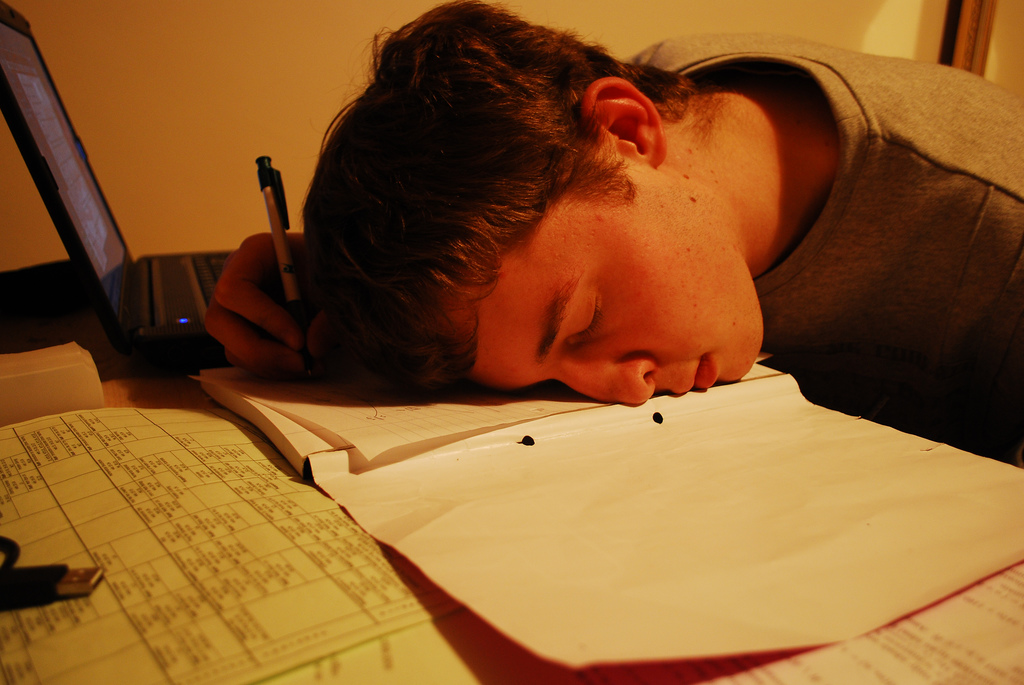
\includegraphics[width=0.95\textwidth]{/part02/Z_is_forZzzzzzzz.jpg}
 \begin{center}
 {\large ``225/365 Z is for Zzzzzzzzzzz''}\par
 Foto di stuartpilbrow\par
 \url{http://www.flickr.com/photos/stuartpilbrow/3326749916/}\par
 Licenza: Attribuzione 2.0 Generico (CC BY 2.0)\par
 \end{center}
\clearpage
\cleardoublepage
 
% (c)~2012 Dimitrios Vrettos - d.vrettos@gmail.com
% (c)~2014 Claudio.carboncinii - claudio.carboncini@gmail.com
\chapter{Equazioni di secondo grado}
\section{Le equazioni di secondo grado in una incognita}

Consideriamo il seguente problema: ``in un triangolo rettangolo l'ipotenusa è più lunga del cateto minore di $4\unit{cm}$, mentre l'altro cateto è più lungo del cateto minore di $2\unit{cm}$. Si vogliono determinare le misure dei tre lati''.

Si può formalizzare il problema indicando con $x$ la misura incognita del cateto minore. La lunghezza dell'ipotenusa sarà $x + 4$, mentre quella dell'altro cateto $x + 2$. Applicando il teorema di Pitagora si ha: $x ^{2 } + ( x + 2 ) ^{2 } = ( x + 4 ) ^{2 }$. Dopo aver effettuato i calcoli e aver portato tutti i termini a sinistra del predicato uguale abbiamo: $x ^{2}-4x-12=0$.
\begin{center}
% (c) 2013 Claudio Carboncini - claudio.carboncini@gmail.com
\begin{tikzpicture}[x=10mm,y=10mm,font=\small]
  \draw (1,1) -- (1,3) -- (2.5,1) -- cycle;
  \node [label={[name=label node]left:$x+2$}] at (1,2) {};
  \node [label={[name=label node]left:$x+4$}] at (3,2) {};
  \node [label={[name=label node]below:$x$}] at (1.75,1) {};
\end{tikzpicture}

\end{center}
Questa è una equazione di secondo grado in una incognita in quanto la variabile $x$ vi compare elevata al secondo grado.
\begin{definizione}
Si dice \emph{equazione di secondo grado}, un'equazione del tipo: $a x ^{2} + b x + c = 0$ con $a$, $b$, $c \in \insR$ e $a \neq 0$. I valori $a$, $b$, $c$ prendono il nome di \emph{coefficienti} e, in particolare, $c$ viene detto \emph{termine noto}.
\end{definizione}

Un'equazione di secondo grado si definisce:
\begin{description*}
 \item \emph{monomia} quando il secondo e il terzo coefficiente sono nulli: $\:a x ^{2}=0$;
 \item \emph{(incompleta) pura} quando il secondo coefficiente è nullo: $\:a x ^{2} + c = 0$;
 \item \emph{(incompleta) spuria} quando il terzo coefficiente è nullo: $\:a x ^{2} + b x = 0$;
 \item \emph{completa} quando i tre coefficienti sono tutti diversi da zero: $\:a x ^{2} + b x + c = 0$.
\end{description*}

\subsection{Risoluzione di un'equazione di secondo grado incompleta pura}

Il coefficiente della $x$ è nullo e l'equazione si presenta nella forma: $ax ^{2 } + c = 0$.
Si risolve portando al secondo membro il termine noto e dividendo per il coefficiente di $x^2$:
\[a x ^{2} + c = 0 \quad\Rightarrow\quad a x ^{2 } = - c \quad\Rightarrow\quad x
^{2} = - \frac{c }{a } \quad\Rightarrow\quad x _{1\text{,}2} = \pm \sqrt{- \frac{c}{a}}.\]
\pagebreak
\begin{exrig}
\begin{esempio}
 Risoluzione di equazioni pure.
\begin{itemize}
\item $4 x ^{2} - 9 =0$.

Risoluzione: $4 x ^{2 } = + 9 \:\Rightarrow\: x ^{2 } = \frac{9 }{4 }
\:\Rightarrow\: x _{1\text{,}2 } = \pm \sqrt{\frac{9 }{4 } } \:\Rightarrow\: x_{1} = - \frac{3 }{2 } \vee x _{2 } = + \frac{3 }{2 }$.
\item $4 x ^{2 } + 9 = 0$.

Risoluzione: $4 x ^{2 } = -9 \:\Rightarrow\: x ^{2 } = - \frac{9 }{4 }$. L'equazione non ammette soluzioni reali in quanto il quadrato di un numero reale non è mai negativo.
\end{itemize}
\end{esempio}
\end{exrig}

Le soluzioni dell'equazione incompleta pura $ax ^{2 } + c = 0$ dipendono dal segno di
$- \dfrac{c }{a }$:
\begin{itemize*}
\item se $-c/a>0$, ovvero se $a$ e $c$ sono discordi, l'equazione ammette \emph{due soluzioni reali distinte opposte}: $x _{1 } = - \sqrt{- \frac{c }{a}} \vee x_{2}= + \sqrt{-\frac{c}{a}}$;
\item se $-c/a<0$, ovvero se $a$ e $c$ sono concordi, l'equazione \emph{non ammette soluzioni reali};
\item se $-c/a=0$, allora $c =0$, l'equazione ha \emph{due soluzioni reali coincidenti nulle}: $x_{1}=x_{2} =0$.
\end{itemize*}

\vspazio\ovalbox{\risolvii \ref{ese:3.1}, \ref{ese:3.2}, \ref{ese:3.3}, \ref{ese:3.4}}

\subsection{Risoluzione di un'equazione incompleta spuria}

Un'equazione incompleta spuria si presenta nella forma: $a x ^{2} + b x = 0$.
Per risolverla, si raccoglie a fattore comune la
$x$; precisamente $x ( a x + b ) = 0$.
Applicando la legge di annullamento del prodotto si ottiene
$x_{1} = 0$ oppure $ax + b = 0$ da cui $x_{2} = - \dfrac{b}{a}$.
Pertanto un'equazione di questo tipo ha sempre due soluzioni reali distinte di cui una nulla.
\begin{exrig}
\begin{esempio}
Risoluzione di equazioni incomplete spurie.
\begin{itemize}
\item $2 x^{2} - 4 x = 0$.

Raccogliendo a fattor comune si ha: $2 x ( x - 2 ) = 0$ da cui, applicando la legge di annullamento del prodotto, segue $2x = 0 \vee x - 2 = 0$ da cui $x_{1} = 0 \vee x_{2} = 2$;
\item $x ^{2 } + x = 0$.

Raccogliendo $x$ a fattore comune, si ha $x ( x + 1 ) = 0$, da cui, applicando la legge di annullamento del prodotto, segue $x = 0 \vee x + 1 = 0$ da cui $x_{1} = 0 \vee x_{2} = - 1$.
\end{itemize}
\end{esempio}
\end{exrig}
\vspazio\ovalbox{\risolvii \ref{ese:3.5}, \ref{ese:3.6}, \ref{ese:3.7}, \ref{ese:3.8}, \ref{ese:3.9}, \ref{ese:3.10}, \ref{ese:3.11}}

\section{Risoluzione di un'equazione completa}

L'equazione di secondo grado completa si presenta nella forma $a x ^{2} + b x = 0$ e per risolverla si applica una formula che si ottiene utilizzando il metodo del completamento del quadrato:

\begin{tabular}{ll}
equazione completa di secondo grado & $a x^{2} + b x + c=0$\\
si moltiplicano ambo i membri per $4a$ & $4 a^{2} x^{2} + 4 a b x + 4 a c=0$\\
si aggiunge $b^{2}$ ad ambo i membri & $4 a^{2} x^{2} + 4 a b x + 4 a c + b^{2}=b^{2}$\\
si porta $4ac$ al secondo membro & $4 a^{2} x^{2} + 4 a b x + b^{2}=b^{2} - 4 a c$\\
il primo membro risulta il quadrato di un binomio & $( 2 a x + b )^{2}=b^{2} - 4 a c$\\
si pone $k=2ax + b$ e l'equazione diventa pura in $k$ & $k^{2}=b^{2} - 4 a c$\\
si calcolano le soluzioni in $k$ & $k_{1\text{,}2}=\pm \sqrt{b^{2} - 4 a c}$\\
al posto di $k$ si sostituisce $2ax + b$ & $2 a x + b=\pm \sqrt{b^{2} - 4 a c}$\\
si separa il monomio con l'incognita & $2 a x=- b \pm \sqrt{b^{2} - 4 a c}$\\
si risolve rispetto all'incognita $x$ & $x_{1\text{,}2}=\dfrac{- b \pm \sqrt{b^{2} - 4 a c}}{2 a}$\\
\end{tabular}

%\begin{description*}
%\item $a x^{2} + b x + c=0$: equazione completa di secondo grado;
%\item $4 a^{2} x^{2} + 4 a b x + 4 a c=0$: si moltiplicano ambo i membri per $4a$;
%\item $4 a^{2} x^{2} + 4 a b x + 4 a c + b^{2}=b^{2}$: si aggiunge ad ambo i membri $b^{2}$;
%\item $4 a^{2} x^{2} + 4 a b x + b^{2}=b^{2} - 4 a c$: si porta $4ac$ a secondo membro;
%\item $( 2 a x + b )^{2}=b^{2} - 4 a c$: il primo membro risulta il quadrato di un binomio;
%\item $k=2 a x + b$: si sostituisce il binomio $2ax + b$ con la la variabile $k$;
%\item $k^{2}=b^{2} - 4 a c$: l'equazione diventa un'equazione di secondo grado pura in $k$;
%\item $k_{1,2}=\pm \sqrt{b^{2} - 4 a c}$: si calcolano le soluzioni in $k$;
%\item $2 a x + b=\pm \sqrt{b^{2} - 4 a c}$: al posto di $k$ si mette il binomio $2ax + b$;
%\item $2 a x=- b \pm \sqrt{b^{2} - 4 a c}$: si separa il monomio con l'incognita;
%\item $x_{1,2}=\frac{- b \pm \sqrt{b^{2} - 4 a c}}{2 a}$: si risolve l'equazione di primo grado rispetto alla $x$.
%\end{description*}

Da quanto ottenuto possiamo osservare che:
\begin{itemize}
\item la soluzione si ottiene esclusivamente operando sui coefficienti
dell'equazione;
\item il valore dell'incognita si ottiene con due calcoli:
\[x_{1} = \dfrac{- b - \sqrt{b^{2} - 4 ac}}{2 a}\quad\text{e}\quad x_{2} = \dfrac{- b + \sqrt{b^{2} - 4 ac}}{2 a}\;;\]
\item nel calcolo è coinvolta l'estrazione di radice quadrata: l'espressione $b^{2} - 4 ac$ prende il nome di \emph{discriminante} e si è soliti indicarla con il simbolo $\Delta$ (delta).
\end{itemize}

Questa formula può essere applicata anche ai tipi di equazioni incomplete che abbiamo già studiato. Il termine discriminante deriva dal sostantivo latino \emph{discrimen} (divisione, punto di separazione); in effetti, il valore assunto da $\Delta$ permette di effettuare una distinzione tra la tipologia delle soluzioni di un'equazione di secondo grado.
Si possono infatti presentare tre casi:
\begin{itemize}
\item Primo caso: $\Delta=b^{2} - 4 a c > 0$. Il radicale $\sqrt{\Delta}$ è un numero reale e l'equazione ammette \emph{due soluzioni reali e
distinte}: $x_{1}=\dfrac{- b - \sqrt{\Delta}}{2 a} \vee x_{2} = \dfrac{- b + \sqrt{\Delta}}{2 a}$;
\item Secondo caso: $\Delta=b^{2} - 4 a c=0$. Il radicale $\sqrt{\Delta} = 0$, quindi l'equazione ammette \emph{due radici reali e coincidenti}: $x_{1}=x_{2}=- \dfrac{b}{2 a}$;
\item Terzo caso: $\Delta=b^{2} - 4 a c < 0$. Il radicale $\sqrt{\Delta}$ non è un numero reale, quindi l'equazione \emph{non ammette soluzioni reali}.
\end{itemize}

Riassumendo e schematizzando si ha:
\begin{center}
\begin{tabular}{ll}
\toprule
\multicolumn{2}{c} {$a x^{2} + b x + c=0$~~con~~$a \neq 0$}\vspace{1.05ex}\\
Discriminante & Soluzioni\\
\midrule
$\Delta > 0$ & Due soluzioni reali e distinte: $x_{1}=\frac{- b - \sqrt{\Delta}}{2 a} \vee x_{2} = \frac{- b + \sqrt{\Delta}}{2 a}$\\
$\Delta = 0$ & Due soluzioni reali e coincidenti: $x_{1}=x_{2}=- \frac{b}{2 a}$ \\
$\Delta < 0$ & Nessuna soluzione reale: $I.S.=\emptyset$ \\
\bottomrule
\end{tabular}
\end{center}
\pagebreak
\begin{exrig}
\begin{esempio}
Risoluzione di equazioni complete.
\begin{itemize}
\item $3 x^{2} - 5 x + 2=0$.

 $a = + 3$, $b = - 5$, $c = + 2$. Calcolo del discriminante: 
\[\Delta = b^{2} - 4 ac = (-5)^{2}-4\cdot(+3)\cdot(+2) = 25 - 24 = 1.\]
 Poiché $\Delta > 0$ l'equazione ammette due soluzioni reali e distinte 
\[x_{1\text{,}2} = \frac{- b \pm \sqrt{\Delta}}{2 a} \:\Rightarrow\: x_{1\text{,}2} = \frac{- (- 5) \pm \sqrt{1}}{2\cdot(+3)} \:\Rightarrow\: x_{1\text{,}2} = \frac{5 \pm 1}{6} \:\Rightarrow\: x_{1} = 1 \vee x_{2} = \frac{2}{3};\]
\item $4 x^{2} - 12 x + 9=0$.

 $a = + 4$, $b = - 12$, $c = + 9$. Calcolo del discriminante: 
\[\Delta=(-12)^{2} -4\cdot(+4)\cdot(+9)=144 - 144 =0.\] 
Poiché $\Delta = 0$ l'equazione ammette due soluzioni reali coincidenti 
\[x_{1\text{,}2} = - \frac{b}{2 a} \:\Rightarrow\: x_{1\text{,}2} = \frac{-(-12)}{2\cdot(+4)} = \frac{12}{8} \:\Rightarrow\: x_{1} = x_{2} = \frac{3}{2};\]
\item $x^{2} - x + 3=0$.

 $a = + 1$, $b = - 1$, $c = + 3$. Calcolo del discriminante: 
\[\Delta = (-1)^{2} - 4\cdot(+1)\cdot(+3) = 1 - 12 = - 11.\]
Poiché $\Delta < 0$ l'equazione non ammette soluzioni reali.
\end{itemize}
\end{esempio}
\end{exrig}
\vspazio\ovalbox{\risolvii \ref{ese:3.12}, \ref{ese:3.13}, \ref{ese:3.14}, \ref{ese:3.15}, \ref{ese:3.16}, \ref{ese:3.17}, \ref{ese:3.18}, \ref{ese:3.19}}

\subsection{Formula ridotta per equazioni di secondo grado}

Se nell'equazione
$a x^{2} + b x + c=0$ il coefficiente $b$ è un numero pari, conviene applicare una formula, detta \emph{formula ridotta}, che semplifica i calcoli.

Supponiamo $b=2 k$, l'equazione $a x^{2} + b x + c=0$ diventa $a x^{2} + 2 k x + c=0$ e nella formula risolutiva dell'equazione si ottiene:
\[x_{1\text{,}2}=\frac{- 2 k \pm \sqrt{( 2 k )^{2}-4 a c}}{2 a}=\frac{- 2 k \pm 2 \sqrt{k^{2} - a c}}{2 a}=\frac{- k \pm \sqrt{k^{2} - a c}}{a}.\]
Dato che $b=2 k$ si ha $k=\frac{b}{2}$ e quindi la formula che conviene utilizzare quando $b$ è pari è:
\[x_{1\text{,}2}=\frac{-\frac{b}{2} \pm \sqrt{\left(\frac{b}{2} \right)^{2} - a c}}{a}.\]

La quantità sotto radice, uguale a $\dfrac{\Delta}{4}$, è detta anche \emph{discriminante ridotto}.
\pagebreak
\begin{exrig}
\begin{esempio}
 Applicazione della formula ridotta nella risoluzione di equazioni complete.
\begin{itemize}
\item $x^{2} - 4 x + 3=0$.

 Il coefficiente di primo grado è pari, per cui conviene utilizzare la formula ridotta: 
\[x_{1\text{,}2}=\frac{-(-2 ) \pm \sqrt{(-2)^{2}-1\cdot(+3)}}{1}=2 \pm \sqrt{1}\:\Rightarrow\:  x_{1} = 1 \vee x_{2} = 3;\]
\item $- x^{2} - 2 x + 24=0$.

 Applichiamo la formula ridotta: 
\[x_{1\text{,}2}=\frac{- ( - 1 ) \pm \sqrt{( -1 )^{2} - (-1)\cdot(+24)}}{-1}=- 1 \pm \sqrt{25}\:\Rightarrow\: x_{1} = - 6 \vee x_{2} = 4;\]
\item $- 3 x^{2} - 6 x + 12=0$.

 Per prima cosa dividiamo l'equazione per $- 3$. Per il secondo principio di equivalenza, si ha l'equazione equivalente~$x^{2} + 2 x - 4=0$. Poiché il coefficiente della~$x$ è pari si può applicare la formula ridotta: 
\[x_{1\text{,}2}=- 1 \pm \sqrt{1 + 4} = - 1\pm \sqrt{5}\:\Rightarrow\: x_{1} = - 1 + \sqrt{5} \vee x_{2} = - 1 - \sqrt{5}.\]
\end{itemize}
\end{esempio}
\end{exrig}

Quando $b$ è pari e $a = 1$, la formula si dice \emph{ridottissima}: $x_{1\text{,}2}=-\frac{b}{2} \pm \sqrt{\left( \frac{b}{2} \right)^{2} - c}$.
%\newpage
\begin{exrig}
\begin{esempio}
 Applicazione della formula ridottissima nella risoluzione di equazioni complete.
\begin{itemize}
\item $x^{2} - 6 x + 8 = 0$.

Il coefficiente $b$ è pari e il coefficiente $a=1$, quindi possiamo applicare la formula ridottissima $x_{1\text{,}2} = 3 \pm \sqrt{9 - 8}$, quindi $x_{1}=2 \vee x_{2} = 4$.
\end{itemize}
\end{esempio}
\end{exrig}
\vspazio\ovalbox{\risolvii \ref{ese:3.20}, \ref{ese:3.21}, \ref{ese:3.22}, \ref{ese:3.23}, \ref{ese:3.24}}\vspazio

Riassumiamo e schematizziamo la risoluzione di un'equazione di secondo grado:
\begin{center}
\begin{tabular}{llll}
\toprule
\multicolumn{4}{c} {Equazioni incomplete}\vspace{1.05ex}\\
Coefficienti & Tipo & Equazione & Soluzioni\\
\midrule
$b = 0$, $c = 0$ & Monomia & $a x^{2}=0$ & $x_{1}=x_{2}=0$\\
$b = 0$, $c \neq 0$ & Pura & $a x^{2} + c=0$ & $\begin{cases} \IS=\emptyset & \text{ se~~}ac>0 \\ x_{1\text{,}2} = \pm \sqrt{- \frac{c}{a}} & \text{ se~~}ac<0\\ \end{cases}$ \\
% $b = 0$, $c \neq 0$ & Pura & $a x^{2} + c=0$ & \IS=\emptyset $ se $ac>0$\\
% & & & $x_{1\text{,}2} = \pm \sqrt{- \frac{c}{a}}$~~se~$a \cdot c<0$\\
$b \neq 0$, $c = 0$ & Spuria & $a x^{2} + b x=0$ & $x_{1} = 0 \vee x_{2} = - \frac{b}{a}$ \vspace{1.1ex}\\
\toprule
\multicolumn{4}{c} {Equazione completa \, $ax^2+bx+c=0$}\vspace{1.05ex}\\
Discriminante & \multicolumn{2}{l} {Numero soluzioni} & Soluzioni\\
\midrule
$\Delta > 0$ & \multicolumn{2}{l} {Due soluzioni reali e distinte}& $x_{1\text{,}2}=\frac{-b\pm{\sqrt {b^{2}-4ac}}}{2a}$\\
$\Delta = 0$ & \multicolumn{2}{l} {Due soluzioni reali e coincidenti} & $x_{1}=x_{2}=-\frac{b}{2a}$\\
$\Delta < 0$ & \multicolumn{2}{l} {Nessuna soluzione reale}& $\IS=\emptyset$\\
\bottomrule
\end{tabular}
\end{center}

\vspazio\ovalbox{\risolvii \ref{ese:3.25}, \ref{ese:3.26}, \ref{ese:3.27}, \ref{ese:3.28}, \ref{ese:3.29}, \ref{ese:3.30}, \ref{ese:3.31}, \ref{ese:3.32}, \ref{ese:3.33}, \ref{ese:3.34}, \ref{ese:3.35}}

\subsection{Equazioni che si possono risolvere con opportune sostituzioni}

\begin{exrig}
\begin{esempio}
Risoluzione di equazioni con sostituzioni.
\begin{itemize}
\item $( x - 1 )^{2} = 16$.

Sostituendo $x - 1 = t$ l'equazione diventa $t^{2} = 16$, le cui soluzioni sono $t_{1} = - 4 \vee t_{2} = + 4$. Per determinare la $x$ sostituiamo i valori di $t$ trovati nella relazione~$x - 1 = t$. Si ha $x - 1 = - 4 \vee x - 1 = + 4$ quindi l'equazione assegnata ammette le due soluzioni
$x_{1} = - 3 \vee x_{2} = 5$;
\item $( x - 1 )^{2} + 2 ( x - 1 ) = 0$.

Sostituendo $x - 1 = t$ l'equazione diventa $t^{2} + 2t = 0$ le cui soluzioni sono $t ( t + 2 ) = 0 \Rightarrow t_{1} = 0 \vee t + 2 = 0 \Rightarrow t_{2} = - 2$. Sostituendo $x - 1 = t$ si ha $x - 1 = 0 \vee x - 1 = - 2$ quindi l'equazione assegnata ammette le due soluzioni~$x_{1} = - 1 \vee x_{2} = 1$.
\end{itemize}
\end{esempio}
\end{exrig}
\vspazio\ovalbox{\risolvii \ref{ese:3.36}, \ref{ese:3.37}, \ref{ese:3.38}}

\section{Discussione e risoluzione di equazioni numeriche frazionarie}

Un'equazione in cui compare l'incognita al denominatore si chiama \emph{frazionaria o fratta.}

\begin{exrig}
\begin{esempio}
Risolvere la seguente equazione:~~$\dfrac{3 x + 2}{1 + x}=\dfrac{2 x + 3}{x - 2}$.
 \paragraph{Passo I} Determiniamo il $\mcm$ dei denominatori: $\mcm = ( 1 + x ) \cdot ( x - 2 )$.
 \paragraph{Passo II} Imponiamo le \emph{condizioni di esistenza} ($\CE$): $\CE\: x \neq - 1 \wedge x \neq 2$. La ricerca dei valori che risolvono l'equazione si restringe ai numeri reali appartenenti all'insieme, $\Dom = \insR - \{-1$, $2\}$ detto \emph{dominio} dell'equazione o \emph{insieme di definizione} (abbreviato $\ID$).
 \paragraph{Passo III} Applichiamo il primo principio d'equivalenza trasportando al primo membro la frazione del secondo membro $\frac{3 x + 2}{1 + x} - \frac{2 x + 3}{x - 2} = 0$. Riduciamo allo stesso denominatore ($\mcm$): 
\[\frac{( 3 x + 2 ) \cdot ( x - 2 ) - ( 2 x + 3 ) \cdot ( 1 + x )}{( 1 +x ) \cdot ( x - 2 )}=0.\]
 \paragraph{Passo IV} Moltiplichiamo ambo i membri per il $\mcm$, certamente diverso da zero per le condizioni poste; l'equazione diventa: $( 3 x + 2 ) \cdot ( x - 2 ) - ( 2 x + 3 ) \cdot ( 1 + x )=0$.
 \paragraph{Passo V} L'equazione che si ottiene è di secondo grado; portiamo l'equazione alla forma canonica: $3 x^{2} - 6 x + 2 x - 4 - 2 x - 3 - 2 x^{2} - 3 x=0 \:\Rightarrow\: x^{2} - 9 x - 7=0$.
 \paragraph{Passo VI} Calcoliamo il discriminante: $\Delta=b^{2} - 4 a c=81 + 28 = 109$. Il discriminante è positivo quindi l'equazione è determinata e ammette due soluzioni reali distinte: 
\[x_{1\text{,}2}=\frac{9 \pm \sqrt{109}}{2} \quad\Rightarrow\quad x_{1}=\frac{9 - \sqrt{109}}{2} \:\vee\: x_{2}=\frac{9 + \sqrt{109}}{2}.\]
 \paragraph{Passo VII} Confrontiamo le soluzioni con le $\CE$; in questo caso le radici appartengono all'insieme $\Dom$; diciamo che sono accettabili e l'insieme soluzione è: $\IS=\left\{\frac{9 - \sqrt{109}}{2}\text{, }\frac{9 +\sqrt{109}}{2} \right\}$.
 \end{esempio}

 \begin{esempio}
Risolvere la seguente equazione:~~$\dfrac{x^{2}}{x^{2} - 3 x + 2}=\dfrac{x - 2}{x - 1} +\dfrac{1}{x + 2}$.
 \paragraph{Passo I} Determiniamo il $\mcm$ dei denominatori. Scomponiamo in fattori i denominatori. Riscriviamo: $\frac{x^{2}}{( x - 2 ) ( x - 1 )}=\frac{x - 2}{x - 1} +\frac{1}{x + 2}$ il $\mcm$ è $( x - 2 ) ( x - 1 ) ( x + 2 )$.
 \paragraph{Passo II} Imponiamo le Condizioni di Esistenza: $\CE\: x \neq 1 \wedge x \neq 2 \wedge x \neq - 2$ quindi $\Dom = \ID =\insR - \{-2$, $1$, $2\}$
 \paragraph{Passo III} Trasportiamo al primo membro ed uguagliamo a zero; riduciamo allo stesso denominatore ($\mcm$) i membri dell'equazione: 
\[\frac{x^{3} + 2 x^{2} - x^{2} + 3 x - 2 - x^{3} - 2 x^{2} + 4x^{2} + 8 x - 4 x - 8}{( x - 2 ) ( x - 1 ) ( x + 2 )} = 0.\]
 \paragraph{Passo IV} Applichiamo il secondo principio di equivalenza moltiplicando ambo i membri per il $\mcm$, certamente diverso da zero per le condizioni poste in precedenza; l'equazione diventa: $3 x^{2} + 7 x - 10 = 0$.
 \paragraph{Passo V} Calcoliamo il discriminante: $\Delta=b^{2} - 4 a c=49 + 120=169$. Il discriminante è positivo, l'equazione determinata e ammette due soluzioni reali distinte: $x_{1\text{,}2}=\frac{- 7 \pm 13}{6}$ cioè~$x_{1}=-\frac{10}{3} \vee x_{2}=1$.
 \paragraph{Passo VI} Confrontiamo con le $\CE$; in questo caso solo $x_{1}$ appartiene all'insieme $\Dom$; diciamo che l'insieme soluzione è: $\IS=\left\{-\frac{10}{3}\right\}$ mentre $x_{2} = 1$ non è accettabile.
\end{esempio}
\end{exrig}
\vspazio\ovalbox{\risolvii \ref{ese:3.39}, \ref{ese:3.40}, \ref{ese:3.41}, \ref{ese:3.42}, \ref{ese:3.43}, \ref{ese:3.44}, \ref{ese:3.45}, \ref{ese:3.46}, \ref{ese:3.47}, \ref{ese:3.48}, \ref{ese:3.49}, \ref{ese:3.50}, \ref{ese:3.51},}

\vspazio\ovalbox{\ref{ese:3.52}, \ref{ese:3.53}}

\section{Discussione e risoluzione di equazioni letterali}
Ricordiamo la seguente definizione:
\begin{definizione}
Una equazione è \emph{letterale} se i coefficienti dell'incognita sono espressioni letterali, cioè se oltre all'incognita (in genere indicata con
la lettera $x$) compare un'altra lettera (in genere $a$, $b$, $k$, \ldots) detta \emph{parametro}.
\end{definizione}

\begin{exrig}
\begin{esempio}
Data l'equazione $k x^{2} - ( 2 k - 1 ) x + ( k - 3 ) = 0$, discutere, al variare di $k$, la realtà delle sue soluzioni.

L'equazione è letterale di secondo grado nell'incognita $x$, i cui coefficienti dipendono dal parametro $k$. Il parametro $k$ può assumere qualunque valore numerico e l'equazione rappresenta una famiglia di equazioni le cui caratteristiche variano a seconda dei valori attribuiti al parametro. Notiamo subito che se
$k$ assume il valore zero, l'equazione non è più di secondo grado. Se $k$ assume il valore $3$, l'equazione è ancora di secondo grado ma è incompleta (spuria) perché priva del termine noto.

\emph{Discutere} un'equazione letterale significa analizzare come varia il suo insieme delle soluzioni al variare del parametro.

Ricordando la formula $x_{1\text{,}2}=\frac{- b \pm \sqrt{b^{2} - 4 a c}}{2 a}$ in cui compaiono i tre coefficienti $a$, $b$, $c$ possiamo dire che, nel caso considerato:
 \begin{itemize*}
 \item il primo coefficiente è $k$, se $k = 0$ l'equazione diventa $x - 3 = 0$ di primo grado con $\IS = \{3\}$;
 \item il secondo coefficiente è $-2k+1$, se questo è nullo, ossia se $k = \frac{1}{2}$ l'equazione diventa $\frac{1}{2} x^{2} - \frac{5}{2}=0$, equazione pura con due soluzioni reali opposte $x_{1} = - \sqrt{5} \vee x_{2} = \sqrt{5}$;
 \item il terzo coefficiente è $k-3$, se è nullo, cioè se $k = 3$ l'equazione diventa $3 x^{2} - 5 x = 0$, equazione spuria con due soluzioni reali $x_{1} = 0 \vee x_{2} = \frac{5}{3}$.
 \end{itemize*}

Per tutti i valori di $k \in \insR - \left\{ 0\text{, }\frac{1}{2}\text{, }3 \right\}$ l'equazione è completa, pertanto l'esistenza di soluzioni reali dipende dal discriminante $\Delta = \left( - 2 k + 1 \right)^{2} - 4 k \left( k - 3 \right) = 8 k + 1$, quindi
\begin{itemize*}
 \item se $8 k + 1 < 0 \:\Rightarrow\: k < - \frac{1}{8}$ l'equazione non ammette soluzioni reali: $\IS = \emptyset$;
 \item se $8 k + 1 > 0 \:\Rightarrow\: k > - \frac{1}{8}$ l'equazione ammette due soluzioni reali distinte $ x_{1\text{,}2} = \frac{\left(2 k - 1 \right) \pm \sqrt{8 k + 1}}{2 k}$
 \item se $k=- \frac{1}{8}$ l'equazione ammette due soluzioni reali coincidenti $ x_{1} = x_{2}=5$.
\end{itemize*}
Riassumendo e schematizzando si ha:
\begin{center}
\begin{tabular}{lll}
\toprule
\multicolumn{3}{c} {$k x^{2} - ( 2 k - 1 ) x + ( k - 3 ) = 0$~~con~~$k \in \insR$}\vspace{1.05ex}\\
Parametro & Insieme Soluzione & Equazione\\
\midrule
$k = 0$ & $x = 3$ & di primo grado\\
$k = \frac{1}{2}$ & $x_{1} = - \sqrt{5} \vee x_{2} = + \sqrt{5}$ & pura\\
$k = 3$ & $x_{1} = 0 \vee x_{2} = \frac{5}{3}$ & spuria\\
$k \in \insR - \left\{ 0\text{, }\frac{1}{2}\text{, }3 \right\}$ & & completa, $\Delta = 8 k + 1$\\
$k < - \frac{1}{8}$ & $\Delta < 0$ non esistono soluzioni reali, $I.S. = \emptyset$& \\
$k \geq - \frac{1}{8}$ & $\Delta \geq 0$ esistono soluzioni reali & \\
$k > - \frac{1}{8}$ & $x_{1}=\frac{\left( 2 k - 1 \right) - \sqrt{8 k + 1}}{2k}\vee x_{2}=\frac{\left( 2 k - 1 \right) + \sqrt{8 k + 1}}{2 k}$ & \\
$k = - \frac{1}{8}$ & $x_{1} = x_{2}=5$ &\\
\bottomrule
\end{tabular}
\end{center}
\end{esempio}

\begin{esempio}
Data l'equazione $x^2 - 3 x + 1 - k = 0$, discutere, al variare di $k \in \insR$, la realtà delle radici.

Il primo e il secondo coefficiente non dipendono dal parametro $k$, quindi analizziamo il terzo coefficiente. Se $k = 1$ l'equazione diventa un'equazione spuria con due radici reali $x_{1} = 0 \vee x_{2} = 3$. Per tutti i valori di $k$ dell'insieme $\insR - \{1\}$ l'equazione è completa e l'esistenza di soluzioni reali dipende dal discriminante $\Delta = 9 - 4 ( 1 - k ) = 4 k + 5$, quindi:
\begin{itemize*}
 \item se $k < - \frac{5}{4}$ l'equazione non ammette soluzioni reali: $\IS = \emptyset$;
 \item se $k \geq - \frac{5}{4}$ l'equazione ammette due radici reali. Esse sono distinte se $k >-\frac{5}{4}\:\Rightarrow\: x_{1\text{,}2} =\frac{3 \pm\sqrt{4 k +5}}{2}$ e coincidenti se $k=- \frac{5}{4} \:\Rightarrow\: x_{1} = x_{2} = \frac{3}{2}$.
\end{itemize*}
Riassumendo e schematizzando si ha:
\begin{center}
\begin{tabular}{lll}
\toprule
\multicolumn{3}{c} {$x^{2} - 3 x + 1 - k = 0$~~con~~$k \in \insR$}\vspace{1.05ex}\\
Parametro & Insieme Soluzione & Equazione\\
\midrule
$k = 1$ & $x_{1} = 0 \vee x_{2} = 3$ & spuria\\
$k \in \insR - \{1\}$ & & completa, $\Delta = 4 k + 5$\\
$k < - \frac{5}{4}$ & $\Delta < 0$ non esistono soluzioni reali, $I.S. = \emptyset$& \\
$k \geq - \frac{5}{4}$ & $\Delta \geq 0$ esistono soluzioni reali & \\
$k > - \frac{5}{4}$ & $x_{1}=\frac{3 - \sqrt{4 k + 5}}{2} \vee x_{2}=\frac{3 + \sqrt{4 k + 5}}{2}$ & \\
$k = - \frac{5}{4}$ & $x_{1} = x_{2}=\frac{3}{2}$ &\\
\bottomrule
\end{tabular}
\end{center}
\end{esempio}

\begin{esempio}
Discutere l'equazione letterale:~~$\dfrac{x^{2}}{m - 1} + 3 + m=\dfrac{2 m x}{m - 1} \left( 1 +\dfrac{1}{m} \right)$.

L'equazione, pur presentando delle frazioni, è intera in quanto l'incognita $x$ non compare al denominatore. Se~$m = 0$ oppure~$m = 1$ l'equazione è priva di significato, quindi poniamo $\CE\: m \neq 0 \wedge m \neq 1$.

Trasportiamo a sinistra del segno di uguaglianza i termini di destra ed eseguiamo il calcolo nella parentesi: 
\[\frac{x^{2}}{m - 1} + 3 + m - \frac{2 m x}{m - 1} \left( 1 +\frac{1}{m} \right) = 0 \:\Rightarrow\: \frac{x^{2}}{m - 1} + 3 + m - \frac{2 m x}{m - 1} - \frac{2 \cancel{m} x}{m - 1} \cdot \frac{1}{\cancel{m}} = 0.\]
Semplifichiamo $m$ nell'ultimo termine, poiché nelle $\CE m \neq 0$, si ottiene
\[\frac{x^{2}}{m - 1} + 3 + m - \frac{2 mx}{m - 1} - \frac{2 x}{m - 1}=0.\]
Riduciamo allo stesso denominatore $m - 1$ ed eliminiamo il denominatore, essendo $m \neq 1$ per le $\CE$; si ha: $x^{2} + 3 m - 3 + m^{2} - m - 2 m x - 2 x = 0$, che scritta in forma canonica diventa $x^{2} - 2 x ( m + 1 ) + m^{2} + 2 m - 3 = 0$.

\emph{Discussione}
\begin{itemize*}
\item il primo coefficiente, essendo uguale a $1$, non dipende dal valore del parametro~$m$, quindi l'equazione è di secondo grado per qualunque valore di $m \in \insR - \{0$, $1\}$;
\item il secondo coefficiente è $- 2 (m + 1)$: se $m = - 1$ l'equazione diventa $x^{2} - 4 = 0$, equazione pura con due soluzioni reali opposte $x_{1} = - 2 \vee x_{2} = 2$;
\item il terzo coefficiente è $m^{2} + 2 m - 3$: se $m^{2} + 2 m - 3 = 0 \:\Rightarrow\: m = 1 \vee m = - 3$ (non consideriamo il caso $m = 1$ per le $\CE$) l'equazione diventa $x^{2} + 4 x = 0$, equazione spuria con due soluzioni reali $x_{1} = 0 \vee x_{2} = - 4$.
\end{itemize*}
Prima conclusione: per tutti i valori di $m \in \insR -\{0$, $1$, $-1$, $-3\}$ l'equazione è completa e l'esistenza di soluzioni reali dipende dal discriminante. Calcoliamo il discriminante: $\frac{\Delta}{4} = ( m + 1 )^{2} - ( m^{2} + 2 m - 3 ) = 4$; esso risulta indipendente dal valore del parametro~$m$ e sempre positivo, quindi l'equazione ammette sempre due soluzioni reali distinte $x_{1} = m - 1 \vee x_{2} = m + 3$.

Riassumendo in una tabella tutti i risultati ottenuti:
\begin{center}
\begin{tabular}{lll}
\toprule
\multicolumn{3}{c} {$\frac{x^{2}}{m - 1} + 3 + m=\frac{2 m x}{m - 1} \left( 1 + \frac{1}{m} \right)$~~con~~$m \in \insR$}\vspace{1.05ex}\\
Parametro & Insieme Soluzione & Equazione\\
\midrule
$m = 0 \vee m=1$ & & priva di significato\\
$m =-1$ & $x_{1}=- 2 \vee x_{2}=2$ & pura\\
$m = -3$ & $x_{1}=0 \vee x_{2}=- 4$ & spuria\\
$m \in \insR - \{0$, $1$, $-1$, $-3\}$ & $x_{1} = m - 1 \vee x_{2} = m + 3$ & completa: $\Delta = 16$\\
\bottomrule
\end{tabular}
\end{center}
\end{esempio}

\begin{esempio}
Discutere l'equazione parametrica~$\dfrac{k + x}{2 x} \left( \dfrac{k + x}{k - x} + \dfrac{k - x}{k + x} \right)=k + \dfrac{2 k}{k x - x^{2}} - 1$.

L'equazione è fratta, poiché l'incognita $x$ compare nel denominatore. Trasportiamo i termini del secondo membro a sinistra del segno di uguaglianza e scomponiamo in fattori i denominatori: 
\[\frac{k + x}{2 x} \left( \frac{k + x}{k - x} + \frac{k - x}{k +x} \right) - k - \frac{2 k}{x ( k - x )} + 1=0\qquad \CE\: x \neq 0 \wedge x \neq k \wedge x \neq - k.\]
Svolgiamo i calcoli nella parentesi e moltiplichiamo: $\frac{k^{2} + x^{2}}{x ( k - x )} - k - \frac{2 k}{x ( k - x )} + 1=0$;
Riduciamo allo stesso denominatore ed eliminiamo il denominatore: $k x^{2} + k x \cdot ( 1 - k ) + k \cdot ( k - 2 )=0$;

\emph{Discussione}
\begin{itemize}
 \item Il primo coefficiente è $k$, se $k = 0$ le $\CE$ si riducono a $x \neq 0$ e l'equazione diventa $0x = 0$ indeterminata, quindi $I.S. = \insR - \{ 0\}$ per le condizioni poste sull'incognita. Avendo studiato il caso $k=0$, possiamo ora supporre $k \neq 0$. Dividiamo tutti i coefficienti per $k$, l'equazione diventa $x^{2} + x \cdot ( 1 - k ) + ( k - 2 )=0$;
 \item il secondo coefficiente è $1-k$, se $k = 1$ le $\CE$ sono $x \neq 0 \wedge x \neq 1 \wedge x \neq - 1$ e l'equazione diventa $x^{2} - 1 = 0$, le soluzioni sono $x_{1} = -1 \vee x_{2} = 1$ che non sono accettabili per le $\CE$;
 \item il terzo coefficiente è $k-2$, se $k = 2$ le $\CE$ sono $x \neq 0 \wedge x \neq 2 \wedge x \neq - 2$ e l'equazione diventa $x^{2} - x = 0$ le cui soluzioni sono $x_{1} = 0 \vee x_{2} = 1$ di cui $x_{1} = 0$ non è accettabile per le $\CE$
\end{itemize}
Per $k \in \insR - \{0$, $1$, $2\}$ l'equazione è completa, l'esistenza di soluzioni reali dipende dal discriminante $\Delta = (1 - k)^{2}-4(k-2)=(k-3)^{2}$, essendo
$\Delta \geq 0\; \forall k$, si avranno sempre due soluzioni reali: coincidenti se $k = 3 \:\Rightarrow\: x_{1} = x_{2} = 1$ accettabili essendo le
$\CE\: x \neq - 3 \wedge x \neq 0 \wedge x \neq 3$; distinte se $k \neq 3 \:\Rightarrow\: x_{1} = 1 \vee x_{2} = k - 2$ e, confrontando con le $\CE$, si $x_{1} = 1$
non è accettabile se $k = - 1$, mentre $x_{2}$ è sempre accettabile per $\forall k \in \insR - \{0$, $1$, $2$, $3$, $-1\}$.

Riassumendo in una tabella tutti i risultati ottenuti:
\begin{center}
\begin{threeparttable}
\begin{tabular}{llll}
\toprule
\multicolumn{4}{c} {$\frac{k + x}{2 x} \left( \frac{k + x}{k - x} + \frac{k - x}{k + x} \right)=k + \frac{2 k}{k x - x^{2}} - 1$~~con~~$k \in \insR$}\vspace{1.05ex}\\
Parametro & Incognita & Insieme Soluzione & Equazione\\
\midrule
 & $x \neq -k \wedge x \neq 0 \wedge x \neq k$ & & \\
$k = 0$ & $x \neq 0$ & $\IS= \insR - \{ 0\}$ & indeterm.\\
$k = 1$ & $x \neq -1 \wedge x \neq 0 \wedge x \neq 1$ & $[x_{1} = - 1 \vee x_{2} = 1]^{*}$ & pura\\
$k = 2$ & $x \neq -2 \wedge x \neq 0 \wedge x \neq 2$ & $x_{1} = 0^{*} \vee x_{2} = 1$ & spuria\\
$k \in \insR - \{0$, $1$, $2\}$ & & & completa\\
$k = 3$ & $x \neq - 3 \wedge x \neq 0 \wedge x \neq 3$ & $x_{1} = x_{2} = 1$ & \\
$k \in \insR - \{0$, 1, 2, $3\}$ & $x \neq - k \wedge x \neq 0 \wedge x \neq k$ & $x_{1} = 1 \vee x_{2} = k - 2$ & \\
$k = - 1$ & & $x_{1} = 1^{*}$ & \\
$k \in \insR -\{-1$, 0, 1, 2, $3\}$ & & $x_{2} = k - 2$ & \\
\bottomrule
\end{tabular}
\begin{tablenotes}
\item [*] La soluzione o le soluzioni non sono accettabili.
\end{tablenotes}
\end{threeparttable}
\end{center}
\end{esempio}
\end{exrig}
\vspazio\ovalbox{\risolvii \ref{ese:3.54}, \ref{ese:3.55}, \ref{ese:3.56}, \ref{ese:3.57}, \ref{ese:3.58}, \ref{ese:3.59}, \ref{ese:3.60}, \ref{ese:3.61}, \ref{ese:3.62}, \ref{ese:3.63}, \ref{ese:3.64}, \ref{ese:3.65}, \ref{ese:3.66}}

\section{Relazioni tra soluzioni e coefficienti}

Consideriamo una generica equazione di secondo grado $a x^{2} + b x + c = 0$ nell'ipotesi in cui ammetta soluzioni reali (cioè $\Delta \geq 0$), sommiamo e moltiplichiamo le soluzioni (o radici) dell'equazione:
\begin{align*}
& x_{1} + x_{2} = \frac{- b - \sqrt{\Delta}}{2 a} + \frac{- b + \sqrt{\Delta}}{2 a} = - \frac{\cancel{2} b}{\cancel{2} a}=- \frac{b}{a};\\
& x_{1} \cdot x_{2}=\left( \frac{- b - \sqrt{\Delta}}{2 a} \right) \cdot \left( \frac{- b + \sqrt{\Delta}}{2 a} \right)= \frac{b^{2} - \Delta}{4 a^2}=\frac{\cancel{b^{2}} + 4 a c - \cancel{b^{2}}}{4 a^{2}} =\frac{\cancel{4 a} c}{\cancel{4} a^{\cancel{2}}}=\frac{c}{a}.
\end{align*}
Quindi, la somma delle radici è $x_{1} + x_{2}=- \dfrac{b}{a}$ e il prodotto delle radici è $x_{1} \cdot x_{2}=\dfrac{c}{a}$.

Osserviamo che queste relazioni tra radici e coefficienti dell'equazione valgono anche nel caso in cui le radici non siano reali ($\Delta<0$).
\begin{exrig}
\begin{esempio}
Determinare somma e prodotto delle soluzioni dell'equazione $a x^{2} + b x +c = 0$, nei casi seguenti, senza risolverla.
 \begin{itemize}
 \item $2 x^{2} + 11 x - 3 = 0$.

 Calcolo il discriminante $\Delta = 145 > 0$ pertanto le radici sono reali e distinte. Applicando le precedenti formule si ha: 
\[x_{1} + x_{2} = - \frac{11}{2}\quad\text{ e }\quad x_{1} \cdot x_{2} = - \frac{3}{2}.\]

 \item $x^{2} \sqrt{2} + 3 x - 2 \sqrt{2} = 0$.
 
 Calcolo il discriminante $\Delta = 25 > 0$ pertanto le radici sono reali e distinte. Applicando le precedenti formule si ha: 
\[x_{1} + x_{2} = - \frac{3}{\sqrt{2}} = - \frac{3 \sqrt{2}}{2}\quad\text{ e }\quad x_{1} \cdot x_{2} = - \frac{2 \sqrt{2}}{\sqrt{2}} = - 2.\]

 \item $x^{2} + 2 x + 15 = 0$.

 Calcolo il discriminante $\Delta = - 56 < 0$ pertanto le radici non sono reali anche se la loro somma e il loro prodotto sono reali, infatti applicando le precedenti formule si ha: $x_{1} + x_{2} = - 2$ e~~$x_{1} \cdot x_{2} = 15$.

 \item $x^{2} - 12 x + 36 = 0$.

 Il discriminate $\Delta = 12^{2} - 4 \cdot 36 = 144 - 144 = 0$. Le radici sono coincidenti, applicando la formula risolutiva si ha $x_{1} = x_{2} = 6$. Applicando le formule per calcolare somma e prodotto si ha $x_{1} + x_{2} = 12$ e $x_{1} \cdot x_{2} = 36$ da cui si conclude ugualmente che $x_{1} = x_{2} = 6$.
 \end{itemize}
\end{esempio}

\begin{esempio}
Determina le radici dell'equazione $x^{2} + 2 x - 15 = 0$ senza applicare la formula risolutiva, ma sfruttando la somma e il prodotto delle radici stesse.

Calcolo il discriminante $\Delta = 64$, le radici sono reali. Esse hanno come somma~$- \frac{b}{a} = -2$ e come prodotto $\frac{c}{a} = -15$.

Le coppie di interi che hanno per prodotto $-15$ sono $(5;-3)$, $(-5;3)$, $(15;-1)$ e $(-15;1)$. Tra tutte queste coppie l'unica che ha per somma $-2$ è la coppia $(-5;3)$.
Pertanto le soluzioni dell'equazione sono $x_{1} = -5 \vee x_{2} = 3$.
\end{esempio}

\begin{esempio}
Si determini la relazione che lega i coefficienti della generica equazione di secondo grado alla somma dei reciproci delle radici.

Si vuole cioè esprimere $\frac{1}{x_{1}} + \frac{1}{x_{2}}$ attraverso i coefficienti $a$, $b$, $c$ dell'equazione generica. Osserviamo in via preliminare che tale somma è possibile con la condizione $x_{1} \neq 0 \wedge x_{2} \neq 0$ che implica $c \neq 0$. Si ha: 
\[\frac{1}{x_{1}} + \frac{1}{x_{2}} = \frac{x_{2} + x_{1}}{x
_{1} \cdot x_{2}} = \frac{- \frac{b}{a}}{\frac{c}{a}} = - \frac{b}{c}.\]
\end{esempio}

\begin{esempio}
Si determini la relazione che lega i coefficienti della generica equazione di secondo grado alla differenza delle radici.

Poiché non abbiamo informazioni a priori su quale delle due soluzioni sia la maggiore, calcoliamo il valore assoluto della differenza richiesta. Il calcolo diventa: \[
\left\lvert x_{1} - x_{2} \right\rvert = \left\lvert \frac{- b -\sqrt{\Delta}}{2 a} - \frac{- b + \sqrt{\Delta}}{2 a} \right\rvert =\left\lvert - \frac{2 \sqrt{\Delta}}{2 a} \right\rvert = \left\lvert -\frac{\sqrt{\Delta}}{a} \right\rvert = \left\lvert -\frac{\sqrt{b^2-4ac}}{a} \right\rvert.
\]
\end{esempio}
\end{exrig}
\vspazio\ovalbox{\risolvii \ref{ese:3.67}, \ref{ese:3.68}, \ref{ese:3.69}, \ref{ese:3.70}, \ref{ese:3.71}, \ref{ese:3.72}, \ref{ese:3.73}, \ref{ese:3.74}, \ref{ese:3.75}, \ref{ese:3.76}}

\subsection{Determinare due numeri conoscendone la somma e il prodotto}

Consideriamo la generica equazione di secondo grado $a x^{2} + bx + c = 0$ nell'ipotesi in cui ammetta soluzioni reali $x_{1}$ e $x_{2}$. Essendo $a \neq 0$, è possibile dividere ambo i membri per $a$, ottenendo: $x^{2} + \dfrac{b}{a} x + \dfrac{c}{a} = 0$. Dato che, per quanto visto precedentemente, $s = x_{1} + x_{2} = - \dfrac{b}{a}$ e $p = x_{1} \cdot x_{2} = \dfrac{c}{a}$, si ha $x^{2} - s x + p = 0$.

Tale equazione risolve quindi la classe di problemi del tipo: ``determinare due numeri la cui somma è $s$ e il cui prodotto è $p$''.

Dall'equazione $x^{2} - s x + p = 0$ discende che tali numeri esistono e sono reali se e solo se $\Delta =s^{2}-4p\geq 0$ ovvero se il quadrato della somma è maggiore o uguale al quadruplo del loro prodotto.
\pagebreak
\begin{exrig}
\begin{esempio}
Determinare due numeri che sommati danno $12$ e moltiplicati danno $35$.

L'equazione che risolve il problema è: $x^{2} - 12 x + 35 = 0$. Le soluzioni sono $x_{1} = 5 \vee x_{2} = 7$.
\end{esempio}

\begin{esempio}
Determinare due numeri che sommati danno $5$ e moltiplicati danno $9$.

L'equazione che risolve il problema è: $x^{2} - 5 x + 9 = 0$. Poiché $\Delta = s^{2} - 4 p = 25 - 36 = - 11$, l'equazione non ammette soluzioni reali e, di conseguenza, non esistono due numeri reali aventi la somma e il prodotto richiesti.
\end{esempio}
\end{exrig}
\vspazio\ovalbox{\risolvii \ref{ese:3.77}, \ref{ese:3.78}, \ref{ese:3.79}, \ref{ese:3.80}}

\subsection{Problemi di natura geometrica di secondo grado}

\begin{problema}
Determinate la misura della diagonale di un rettangolo avente il perimetro di $80\unit{m}$ e l'area di $375\unit{m^2}$.
\end{problema}

\begin{center}
 % (c) 2013 Claudio Carboncini - claudio.carboncini@gmail.com
\begin{tikzpicture}[x=10mm,y=10mm,font=\small]
  \draw (1,1) rectangle (5,2);
  \draw (1,1)--(5,2);
  
  \node [label={[name=label node]left:$A$}] at (1,1) {};
  \node [label={[name=label node]left:$D$}] at (1,2) {};
  \node [label={[name=label node]right:$C$}] at (5,2) {};
  \node [label={[name=label node]right:$B$}] at (5,1) {};

%  \foreach \x in {1,5}
%    \foreach \y in {1,2}
%      \filldraw[fill=black, draw=black]  (\x,\y) circle (1pt);

\end{tikzpicture}

\end{center}

\emph{Dati}: $2p = 2(\overline{AB}+\overline{BC})= 80\unit{m}$, $\Area = 375\unit{m^2}$.

\emph{Obiettivo}: $\overline{AC}$.

\begin{soluzione}

$\overline{AC} = \sqrt{\overline{AB}^{2} + \overline{BC}^{2}}$ per il teorema di Pitagora applicato al triangolo $ABC$ retto in $B$.

Sono incognite le misura dei lati, quindi poniamo $\overline{AB}=x$ e $\overline {BC}=y$ con $x>0$ e $y>0$.

Il problema si formalizza con il sistema:
$\left\{ \begin{array}{l} x + y = 40 \\x \cdot y = 375 \end{array}\right.$
che esprime la ricerca di due numeri nota la loro somma $40$ e il loro prodotto $375$. I numeri richiesti sono le soluzioni reali positive dell'equazione $t^{2} - 40 t + 375 = 0$ e precisamente $t_{1} = 15 \vee t_{2} = 25$.

Per come abbiamo disegnato la figura abbiamo quindi: $\overline{AB} = 25\unit{m}$ e $\overline{BC} = 15\unit{m}$, da cui $\overline{AC} = \sqrt{\overline{AB}^{2} + \overline{BC}^{2}} =\sqrt{850} = 5 \sqrt{34}\unit{m}$.
\end{soluzione}
\vspazio\ovalbox{\risolvii \ref{ese:3.81}, \ref{ese:3.82}, \ref{ese:3.83}}

\section{Scomposizione del trinomio di secondo grado}

Si consideri il trinomio di secondo grado: $a x^{2} + b x + c$ e sia $a x^{2} + b x + c = 0$ (con $\Delta \geq 0$) l'equazione associata a tale trinomio. Effettuiamo le seguenti operazioni:
\begin{itemize*}
\item si mette in evidenza $a$: $a x^{2} + b x + c = a \left( x^{2} + \frac{b}{a} x + \frac{c}{a} \right)$;
\item si sostituiscono le relazioni trovate nel precedente paragrafo riguardo la somma e il prodotto delle soluzioni $x_{1}$ e $x_{2}$: $a \left( x^{2} + \frac{b}{a} x + \frac{c}{a} \right) = a \left[x^{2} - ( x_{1} + x_{2} ) x + x_{1} \cdot x_{2} \right]$;
\item si svolgono i calcoli nella parentesi quadra:
\[a \left[ x^{2} - ( x_{1} + x_{2} ) x + x_{1} x_{2}\right] = a\left[ x^{2} - x_{1} x - x_{2} x + x_{1} x_{2}\right];\]
\item si effettua il raccoglimento parziale e si ottiene:
\[a \left[x^{2} - x_{1} x - x_{2} x + x_{1} x_{2}\right] = a \left[ {x \left(x - x_{1} \right) - x_{2} \left( x - x_{1}\right)}\right] = a \left( x - x_{1} \right) \left( x - x_{2} \right).\]
\end{itemize*}

Sulla base del segno di $\Delta$ è possibile distinguere i casi illustrati in tabella:
\begin{center}
\begin{tabular*}{.9\textwidth}{@{\extracolsep{\fill}}*{3}{l}}
\toprule
Discriminante & Soluzioni & Scomposizione \\
\midrule
Caso I:\quad $\Delta > 0$ & $x_{1} \neq x_{2}$ & $a x^{2} + b x + c=a ( x - x_{1} ) ( x - x_{2} )$\\
Caso II:\quad $\Delta = 0$ & $x_{1} = x_{2}$ & $a x^{2} + b x + c=a ( x - x_{1} )^{2}$ \\
Caso III:\quad $\Delta < 0$ & $x_{1}$, $x_{2} \notin \insR$ & $a x^{2} + b x + c$\quad è irriducibile \\
\bottomrule
\end{tabular*}
\end{center}
\begin{exrig}
\begin{esempio}
Scomporre in fattori i seguenti trinomi.
\begin{itemize}
\item $x^{2} - 5 x + 6$.

Calcolo le soluzioni dell'equazione $x^{2} - 5 x + 6 = 0$. Si ha $x_{1\text{,}2} = \dfrac{5 \pm \sqrt{25 - 24}}{2}$, cioè $x_{1} = 2 \vee x_{2} = 3$. Applicando la formula ottenuta nel caso I si ha: \[x^{2} - 5 x + 6=( x - 2 ) ( x - 3 ).\]
\item $x^{2} - 12 x + 36$.

Poiché $\Delta = 144 - 144 = 0$ il trinomio è un quadrato di un binomio e applicando la formula ottenuta nel caso II si ha: $x^{2} - 12 x + 36=( x - 6 )^{2}$.
\item $2 x^{2} + 3 x + 5$.

Essendo $\Delta=9 - 40=-31$, il trinomio è irriducibile.
\item $- 5 x^{2} + 2 x + 1$.

Calcolo le radici dell'equazione associata $- 5 x^{2} + 2 x + 1 = 0$: $x_{1\text{,}2} = \frac{- 2 \pm \sqrt{24}}{- 10} = \frac{1 \pm \sqrt{6}}{5}$ quindi $x_{1} = \frac{1 - \sqrt{6}}{5} \vee x_{2} = \frac{1 + \sqrt{6}}{5}$ e scrivo la scomposizione: \[- 5 x^{2} + 2 x + 1=- 5 \left( x - \frac{1 - \sqrt{6}}{5} \right) \left( x - \frac{1 + \sqrt{6}}{5} \right).\]
\end{itemize}
\end{esempio}

\begin{esempio}
Scrivere un'equazione di secondo grado che ammetta le seguenti soluzioni $x_{1} = \frac{1}{2}$ e $x_{2} = 3$.

Per quanto visto nel paragrafo, si ha
\begin{align*}
&\left(x-\frac{1}{2} \right) \left(x + 3 \right)=0\\
\Rightarrow\: & x^{2} + 3 x-\frac{1}{2} x - \frac{3}{2}=0\\
\Rightarrow\: & x^{2} + 5 x - \frac{3}{2}=0\\
\Rightarrow\: & 2 x^{2} + 5 x-3=0
\end{align*}
\end{esempio}
\end{exrig}

\osservazione
Si vuole scomporre in fattori il trinomio $m = 4 x^{2} + 2 x - 6$, avente tutti i coefficienti pari. Anche se osserviamo che tutti i suoi coefficienti sono pari, non possiamo dividire per due, non essendo un'equazione. Il polinomio $m = 2 x^{2} + x - 3$ è diverso da quello assegnato, mentre le equazioni associate all'uno e all'altro sono equivalenti. Nel procedere alla scomposizione, una volta trovate le radici, per ottenere le quali possiamo anche usare l'equazione equivalente $2 x^{2} + x - 3 = 0$, è necessario moltiplicare per $a$. Quindi, in questo caso le radici sono $x_{1} = - \frac{3}{2} \vee x_{2} = 1$ e pertanto il trinomio assegnato si scompone come: $4 x^{2} + 2 x - 6 = 4 \left( x + \frac{3}{2} \right) ( x - 1)$.

\vspazio\ovalbox{\risolvii \ref{ese:3.84}, \ref{ese:3.85}, \ref{ese:3.86}, \ref{ese:3.87}}

\section{Regola di Cartesio}

Se in un'equazione di secondo grado i coefficienti sono tutti diversi da zero e il discriminante è non negativo, è possibile avere delle informazioni sui
segni delle soluzioni senza calcolarle esplicitamente.

In un'equazione $a x^{2} + b x + c = 0$, dove i coefficienti sono tutti non nulli, le coppie di coefficienti $(a;b)$ e~$(b;c)$ sono dette coppie di \emph{coefficienti consecutivi}. Una coppia di coefficienti consecutivi presenta:
\begin{itemize*}
\item una \emph{permanenza} se i coefficienti hanno lo stesso segno;
\item una \emph{variazione} se i coefficienti hanno segni diversi.
\end{itemize*}

\begin{exrig}
\begin{esempio}
Determinare le variazioni e le permanenze nelle seguenti equazioni:
\begin{center}
\begin{tabular*}{.9\textwidth}{@{\extracolsep{\fill}}*{10}{c}}
\toprule
Equazione & $a$ & & & & $b$ & & & & $c$ \\
\midrule
$2 x^{2} - 3 x - 1$ & $+$ & $\rightarrow$ & variazione & $\leftarrow$ & $-$ & $\rightarrow$ & permanenza & $\leftarrow$ & $-$\\
$- x^{2} - 3 x - 1$ & $-$ & $\rightarrow$ & permanenza & $\leftarrow$ & $-$ & $\rightarrow$ & permanenza & $\leftarrow$ & $-$\\
$- 3 x^{2} + 4 x - 1$ & $-$ & $\rightarrow$ & variazione & $\leftarrow$ & $+$ & $\rightarrow$ & variazione & $\leftarrow$ & $-$\\
$2 x^{2} + x - 1$ & $+$ & $\rightarrow$ & permanenza & $\leftarrow$ & $+$ & $\rightarrow$ & variazione & $\leftarrow$ & $-$\\
\end{tabular*}
\end{center}

\end{esempio}
\end{exrig}

\begin{teorema}[di Cartesio]
In un'equazione di secondo grado $a x^{2} + b x + c = 0$ con $a$, $b$, $c \neq 0$ e $\Delta \geq 0$, il numero di radici positive è uguale al numero di variazioni presenti nelle coppie di coefficienti consecutivi. Se vi è una sola variazione, le radici sono discordi e il valore assoluto maggiore è quello della radice positiva se la variazione è nella coppia $(a;b)$, mentre è della radice negativa se la variazione è nella coppia $(b;c)$.
\end{teorema}

\begin{exrig}
\begin{esempio}
Determinare il segno delle soluzioni dell'equazione $x^2 + 2 x - 3 = 0$ senza risolverla.

L'equazione $x^2 + 2 x - 3 = 0$ ha soluzioni reali in quanto $\Delta = 16 > 0$. Dal momento che vi è una sola variazione, quella della coppia $(b;c)$, l'equazione ha radici discordi e il valore assoluto maggiore è quello della radice negativa.

Dimostriamo quanto è stato affermato tenendo presente che $x_{1} + x_{2} = - \frac{b}{a}$ e $x_{1}\cdot x_{2} = \frac{c}{a}$; nell'equazione proposta si ha:
$x_{1} + x_{2} = - 2$ e $x_{1} \cdot x_{2} = - 3$ dunque prodotto negativo e somma negativa. Il prodotto di due numeri è negativo quando i fattori sono discordi, quindi una soluzione è positiva e una è negativa. Chiamiamo $x_1$ la soluzione negativa e $x_2$ la soluzione positiva, poiché $x_{1} + x_{2} = - 2 < 0$ deduciamo che in valore assoluto è più grande il numero negativo, cioè $\valass{x_{1}} > \valass{x_{2}}$.
\end{esempio}

\begin{esempio}
Determinare il segno delle soluzioni delle seguenti equazioni senza risolverle.
\begin{itemize}
	\item $2 x^{2} - 6 x - 56 = 0$. L'equazione ha soluzioni reali in quanto $\Delta = 484 > 0$; dal momento che vi è una sola variazione le radici sono discordi
	e il valore assoluto maggiore è quello della radice positiva poiché che la variazione è nella coppia $(a;b)$.
	\item $-3 x^{2} - 24 x - 21 = 0$. L'equazione ha soluzioni reali in quanto $\Delta = 324 > 0$; dal momento che non vi sono variazioni, l'equazione ha due radici negative.
	\item $x^{2} - 10 x + 25 = 0$. L'equazione ha due soluzioni coincidenti in quanto $\Delta = 0$; dal momento che vi sono due variazioni, le due radici coincidenti sono positive.
\end{itemize}
\end{esempio}
\end{exrig}
\vspazio\ovalbox{\risolvii \ref{ese:3.88}, \ref{ese:3.89}, \ref{ese:3.90}}

\section{Equazioni parametriche}

\begin{definizione}

Si definisce \emph{parametrica} un'equazione i cui coefficienti dipendono da un parametro.
\end{definizione}

L'equazione $3 x^{2} + ( k - 1 ) x + 2 - 3 k= 0$ è parametrica di secondo grado nell'incognita $x$; i suoi coefficienti dipendono dal valore del parametro $k$ e quindi la natura e il segno delle sue soluzioni dipendono da $k$.

In molti problemi di applicazione della matematica in situazioni reali in cui compare un parametro, non interessa tanto determinare le soluzioni dell'equazione che formalizza il problema, quanto sapere se le soluzioni hanno determinate caratteristiche.
Sappiamo che attraverso i coefficienti di un'equazione di secondo grado si possono determinare alcune relazioni tra le sue soluzioni:
\begin{itemize*}
\item soluzioni reali se $\Delta = b^{2} - 4 a c \geq 0$; reali coincidenti se $\Delta = 0$, reali distinte se $\Delta > 0$;
\item la somma delle soluzioni è $x_{1} + x_{2} = - \dfrac{b}{a}$;
\item il prodotto delle soluzioni è $x_{1} \cdot x_{2} = \dfrac{c}{a}$.
\end{itemize*}

Nell'equazione $3 x^{2} + ( k - 1 ) x + 2 - 3 k = 0$ si ha $\Delta = ( k - 1 )^{2} - 12 ( 2 - 3 k )$ dipendente dal parametro $k$.
Dall'analisi del $\Delta$ si potranno dedurre quali condizioni deve verificare $k$ affinché esistano soluzioni reali. Analizzando somma e prodotto
$x_{1} + x_{2} = - \frac{( k - 1 )}{3}$ e $x_{1} \cdot x_{2} =\frac{( 2 - 3 k )}{3}$ potremo stabilire il segno ed altre caratteristiche delle soluzioni.

\begin{exrig}
\begin{esempio}
Assegnata l'equazione $( k + 1 ) x^{2} + ( 2 k + 3 ) x + k = 0$, stabilire per quale valore di $k$
\begin{enumeratea}
\item l'equazione si riduce al primo grado;
\item l'equazione ammette soluzioni reali distinguendo i casi ``soluzioni coincidenti'' e ``soluzioni distinte'';
\item la somma delle soluzioni sia nulla, determinando in tal caso le soluzioni.
\end{enumeratea}
\emph{Svolgimento}
\begin{enumeratea}
\item l'equazione diventa di primo grado se il coefficiente $a$ si annulla, cioè se $k + 1 = 0$ quindi $k = - 1$. In tal caso si ha una sola soluzione reale $ x=1 $;
\item studiamo il segno del discriminante: $\Delta = ( 2 k + 3 )^{2} - 4 k ( k + 1 ) \geq 0$ da cui ricaviamo 
\[4 k^{2} + 12 k + 9 - 4 k^{2} - 4 k \geq 0 \:\Rightarrow\: 8 k + 9 \geq 0.\] 
Pertanto se $k = - \frac{9}{8}$ le soluzioni sono coincidenti, se $k > - \frac{9}{8}$ le soluzioni sono reali distinte, se invece $ k<-\frac{9}{8} $ non ci sono soluzioni reali;
\item dalla formula della somma delle soluzioni ricaviamo $x_{1} + x_{2} = - \frac{( 2 k + 3 )}{( k + 1 )}$ e quindi la somma sarà nulla se $2 k + 3 = 0 \:\Rightarrow\: k = - \frac{3}{2}$. Poiché $- \frac{3}{2} < - \frac{9}{8}$, per $k = - \frac{3}{2}$ non ci sono soluzioni reali, infatti sostituendolo nell'equazione quest'ultima diventa $ x^2+3=0 \Rightarrow x^2=-3$ impossibile!
\end{enumeratea}
\end{esempio}
\end{exrig}
\vspazio\ovalbox{\risolvii \ref{ese:3.91}, \ref{ese:3.92}, \ref{ese:3.93}, \ref{ese:3.94}, \ref{ese:3.95}, \ref{ese:3.96}, \ref{ese:3.97}, \ref{ese:3.98}, \ref{ese:3.99}, \ref{ese:3.100}, \ref{ese:3.101}, \ref{ese:3.102},}

\vspazio\ovalbox{\ref{ese:3.103}, \ref{ese:3.104}, \ref{ese:3.105}, \ref{ese:3.106}, \ref{ese:3.107}, \ref{ese:3.108}, \ref{ese:3.109}, \ref{ese:3.110}, \ref{ese:3.111}}

\section{Problemi di secondo grado in una incognita}

 \epigraph{La risoluzione dei problemi [\ldots] serve ad acuire l'ingegno e a dargli la facoltà di penetrare
 l'intera ragione di tutte le cose.}{{\scshape{R. Descartes}}}

Sappiamo che nel corso degli studi o nell'attività lavorativa possono presentarsi problemi di diversa natura: di tipo economico, scientifico, sociale; possono riguardare insiemi numerici o figure geometriche. La matematica ci può aiutare a risolvere i problemi quando essi possono essere tradotti in ``forma matematica'', quando cioè è possibile trascrivere in simboli le relazioni che intercorrono tra le grandezze presenti nel problema e quando si può costruire, tramite queste relazioni, un modello matematico che ci permetta di raggiungere la soluzione al quesito.

Affronteremo problemi di tipo algebrico o geometrico, che potranno essere formalizzati attraverso equazioni di secondo grado in una sola incognita.
Teniamo presente, prima di buttarci nella risoluzione del problema, alcuni passi che ci aiuteranno a costruire il modello matematico:
\begin{itemize*}
\item la lettura ``attenta'' del testo al fine di individuare l'ambiente del problema, le parole chiave, i dati e le informazioni implicite, l'obiettivo;
\item la scelta della grandezza incognita del problema, la descrizione dell'insieme in cui si ricerca il suo valore, le condizioni che devono essere soddisfatte dall'incognita;
\item la traduzione in ``forma matematica'' delle relazioni che intercorrono tra i dati e l'obiettivo, cioè l'individuazione del modello matematico (equazione risolvente).
\end{itemize*}
Dopo aver risolto l'equazione occorre confrontare la soluzione trovata con le condizioni poste dal problema.

\begin{problema}
Nel triangolo rettangolo $ABC$ rettangolo in $C$, l'ipotenusa $AB$ supera il cateto maggiore $BC$ di $2\unit{m}$; la differenza tra i cateti è $23\unit{m}$. Determinare la misura del perimetro e l'area del triangolo.
\end{problema}

\begin{multicols}{3}
\emph{Dati}

$\overline {AB} = \overline {BC} + 2$;

$\overline {BC} - \overline {AC} = 23$;

$A \widehat {C} B = 90\grado$.

\emph{Obiettivo}

$2p$;

Area.

 % (c) 2013 Claudio Carboncini - claudio.carboncini@gmail.com
\begin{tikzpicture}[x=10mm,y=10mm,font=\small]

  \draw (1,1) -- (1,2) -- (3.5,1) -- cycle;
  \node [label={[name=label node]left:$A$}] at (1,2) {};
  \node [label={[name=label node]right:$B$}] at (3.5,1) {};
  \node [label={[name=label node]left:$C$}] at (1,1) {};

\end{tikzpicture}

\end{multicols}

\begin{soluzione}

Osserva che $2p = \overline {AB} + \overline {BC} + \overline {AC}$ e $\Area =\frac{\overline {BC} \cdot \overline {AC}}{2}$.
Ponendo $\overline {BC} = x$, si ha $\overline {AB} = x + 2$~~e~~$\overline{AC} = x - 23$~~con
$\left\{\begin{array}{l} x > 0 \text{ essendo misura di un segmento} \\x >23 \text{ poiché } \overline {AC} \text{ deve essere positiva}
\end{array}\right.$.

Essendo rettangolo, i lati del triangolo sono legati dal teorema di Pitagora
quindi si deve verificare: $\overline {AB}^{2}= \overline {AC}^{2} + \overline {BC}^{2}\:\Rightarrow\: ( x + 2 )^{2} = ( x - 23 )^{2} + x^{2}$. Sviluppando i calcoli si ottiene l'equazione risolvente di secondo grado, in forma canonica: $x^{2} - 50 x + 525 = 0$ con $\Delta = 400$. L'equazione è quindi determinata pertanto esistono due soluzioni reali distinte: $x_{1} = 15 \vee x_{2} = 35$ entrambe positive. Ai fini del problema $x_{1} = 15$ non è accettabile, quindi il problema ha una sola soluzione: $\overline {BC} = 35 \:\Rightarrow\: \overline {AB} = 37$ e $\overline {AC} = 12$. Conclusione: $2p = 35 + 37 + 12 = 84\unit{m}$~~e~~$\Area = 210\unit{m^{2}}$.
\end{soluzione}

\begin{problema}
Un padre aveva $26$ anni alla nascita del figlio; moltiplicando le età attuali del padre e del figlio si ottiene il triplo del quadrato dell'età del figlio; calcolare le due età.
\end{problema}

Indichiamo con $p$ l'età attuale del padre e con $f$ l'età attuale del figlio.

\emph{Dati}: $p = f + 26$~~e~~$p \cdot f = 3 f^{2}$.

\emph{Obiettivo}: $f$, $p$.

\begin{soluzione}
I dati permettono di impostare la relazione $(f + 26) \cdot f = 3 \cdot f^{2}$ che esprime il legame tra le età di oggi del padre e del figlio; siamo di
fronte ad un'equazione di secondo grado nell'incognita $f$. La soluzione dell'equazione deve essere espressa da un numero positivo poiché esprime l'età.
Risolviamo l'equazione $2 f^{2} - 26 f = 0$ le cui soluzioni sono $f_{1} = 0 \vee f_{2} = 13$. Per le condizioni poste la soluzione del problema è
$f = 13$. Quindi oggi il figlio ha $13$ anni e, di conseguenza, il padre $39$.
\end{soluzione}

\begin{problema}
Il trapezio isoscele $ABCD$ è inscritto in una semicirconferenza di diametro $AB$ di misura $25\unit{cm}$; determina le misure dei lati del trapezio sapendo che il
suo perimetro è $62\unit{cm}$.
\end{problema}

\begin{multicols}{2}
\emph{Dati}

$\overline {AB} = 25$;~~$2p = 62$;

$AB \parallel CD$;~~$\overline {AD} = \overline {BC}$.

\emph{Obiettivo}

$\overline {CD}$;~~$ \overline {BC}$.

 % (c) 2013 Claudio Carboncini - claudio.carboncini@gmail.com
\begin{tikzpicture}[x=10mm,y=10mm,font=\small]
  \coordinate(a) at (-2.5,0);
  \coordinate(d) at (120:2.5);
  \coordinate(e) at (90:2.5);
  \coordinate(c) at (60:2.5);
  \coordinate(b) at (2.5,0);
  \coordinate (h) at ($(a)!(c)!(b)$);%trova le coordinate della proiezione di c su a--b
  \draw (-2.5,0) arc (180:0:2.5) -- cycle;% semicirconferenza e diametro
  \draw (a) -- (d) -- (c) -- (b);%disegna il trapezio
  \draw [dotted] (e) -- (0,0);%da E a O
  \draw [dotted] (c) -- (h);% c--h
  \draw [dotted] (e) -- (b);% e--b
  \node [label={[name=label node]below left:$A$}] at (a) {};
  \node [label={[name=label node]below right:$B$}] at (b) {};
  \node [label={[name=label node]above right:$C$}] at (c) {};
  \node [label={[name=label node]above left:$D$}] at (d) {};
  \node [label={[name=label node]above:$E$}] at (e) {};
  \node [label={[name=label node]below:$H$}] at (h) {};
  \filldraw[fill=black, draw=black]  (a) circle (1pt);
  \filldraw[fill=black, draw=black]  (b) circle (1pt);
  \filldraw[fill=black, draw=black]  (c) circle (1pt);
  \filldraw[fill=black, draw=black]  (d) circle (1pt);
  \filldraw[fill=black, draw=black]  (h) circle (1pt);
  \filldraw[fill=black, draw=black]  (e) circle (1pt);

\end{tikzpicture}

\end{multicols}

\begin{soluzione}
$\overline {AB} + \overline {CD} + 2 \overline {BC} = 62$; fissiamo come incognita $\overline {BC} = x$.
Determiniamo le condizioni sull'incognita: dovrà essere $x > 0$ poiché rappresenta la misura di un segmento e inoltre affinché esista
realmente il trapezio isoscele il punto $C$ non deve coincidere con il punto medio $E$ dell'arco $CD$ cioè $ CB<EB $, quindi $x < \dfrac{25}{2} \sqrt{2}$.

Tracciata l'altezza $CH$ ($H \in AB$) si ha $\overline {CD} = \overline {AB} - 2 \overline {HB}$ e per il 1° teorema di Euclide\footnote{in ogni triangolo rettangolo ciascun cateto è medio proporzionale tra l'ipotenusa e la proiezione del cateto stesso sull'ipotenusa.} sul triangolo~$ACB$, rettangolo in
$C$ (poiché insiste su una semicirconferenza con diametro $AB$), $\overline {HB}: \overline {CB} = \overline {CB} : \overline{AB}$; determiniamo quindi la misura di $HB$ in funzione dell'incognita fissata:
$\overline {HB} = \dfrac{x^{2}}{25}$ da cui $\overline{CD} = 25 - \dfrac{2 x^{2}}{25}$.

Costruiamo l'equazione risolvente: $25 + 2 x + 25 - \dfrac{2 x^{2}}{25} = 62 \:\Rightarrow\: x^{2} - 25 x + 150 = 0$ che ha soluzioni $x_{1} = 10 \vee x_{2} = 15$, entrambe accettabili. Si hanno dunque due trapezi inscritti che risolvono il problema. Poiché $\overline{CD}= 2p-\overline{AB}-2\overline{BC}$ si ha $\overline{CD}=62-25-10=27\unit{cm}$ o $\overline{CD}=62-25-15=22\unit{cm}$.
\begin{center}
 % (c) 2013 Claudio Carboncini - claudio.carboncini@gmail.com
\begin{tikzpicture}[x=10mm,y=10mm,font=\small]
  \coordinate(a) at (-2,0);
  \coordinate(d) at (135:2);
  \coordinate(c) at (45:2);
  \coordinate(b) at (2,0);
  \coordinate(a1) at (3,0);
  \coordinate(d1) at (4,1.732);
  \coordinate(c1) at (6,1.732);
  \coordinate(b1) at (7,0);
  \coordinate(t) at (0,0);
  \coordinate(t1) at (5,0);
  \draw (-2,0) arc (180:0:2) -- cycle;% semicirconferenza e diametro primo trapezio
  \draw (3,0) arc (180:0:2) -- cycle;% semicirconferenza e diametro secondo trapezio
  \draw (a) -- (d) -- (c) -- (b);%disegna il trapezio
  \draw (a1) -- (d1) -- (c1) -- (b1);%disegna il secondo trapezio
  \node [label={[name=label node]below:$A$}] at (a) {};
  \node [label={[name=label node]below:$B$}] at (b) {};
  \node [label={[name=label node]right:$C$}] at (c) {};
  \node [label={[name=label node]left:$D$}] at (d) {};
  \node [label={[name=label node]below:$BC=10\,  cm$}] at (t) {};
  \node [label={[name=label node]below:$A$}] at (a1) {};
  \node [label={[name=label node]below:$B$}] at (b1) {};
  \node [label={[name=label node]right:$C$}] at (c1) {};
  \node [label={[name=label node]left:$D$}] at (d1) {};
  \node [label={[name=label node]below:$BC=15\,  cm$}] at (t1) {};
  \filldraw[fill=black, draw=black]  (a) circle (1pt);
  \filldraw[fill=black, draw=black]  (b) circle (1pt);
  \filldraw[fill=black, draw=black]  (c) circle (1pt);
  \filldraw[fill=black, draw=black]  (d) circle (1pt);
  \filldraw[fill=black, draw=black]  (a1) circle (1pt);
  \filldraw[fill=black, draw=black]  (b1) circle (1pt);
  \filldraw[fill=black, draw=black]  (c1) circle (1pt);
  \filldraw[fill=black, draw=black]  (d1) circle (1pt);

\end{tikzpicture}

\end{center}
\end{soluzione}

\begin{problema}
Un capitale di \officialeuro~$\np{25000}$ viene depositato in banca a un tasso di interesse annuo $c$. Gli interessi maturati durante il primo anno non vengono ritirati.
Nell'anno seguente si investono sia il capitale sia gli interessi maturati a un tasso di interesse annuo aumentato dello $\np{0,5}\%$. Alla fine dei due anni si ritira
la somma di \officialeuro~$\np{26291,10}$. Calcola i tassi di interesse praticati dalla banca.
\end{problema}
Assumiamo come incognita $c$ il tasso di interesse praticato il primo anno, espresso come numero decimale e
non in forma percentuale. Il tasso praticato nel secondo anno sarà $c+\np{0,005}$.

\begin{soluzione}
Alla fine del primo anno in banca si hanno tra capitale e interessi \[\np{25000} + \np{25000} \cdot c = \np{25000} ( 1 + c ).\] Nel secondo anno il tasso praticato è $c+\np{0,005}$ che va applicato alla somma $\np{25000}(1+c)$. Si ottiene quindi l'equazione \[\np{25000} ( 1 + c ) ( 1 + c + \np{0,005} ) = \np{26291,10}.\]
Moltiplicando le parentesi tonde si ha $\np{25000} ( \np{1,005} + c + \np{1,005} c + c^{2} ) = \np{26291,10}$ e poi dividendo per $\np{25000}$ e ordinando otteniamo
$c^{2} + \np{2,005} c - \np{0,046644}=0$ con soluzioni
\[c_{1\text{,}2} = \dfrac{- \np{2,005} \pm \sqrt{\np{4,020025} + \np{0,186576}}}{2} = \dfrac{\np{-2,005} \pm \np{2,051}}{2}\:\Rightarrow\: c_{1} = \np{-2,028} \vee c_{2} = \np{0,023}.\]
La soluzione $c_1$ è negativa e pertanto non accettabile. La risposta al problema è $\np{0,023}$ cioè $\np{2,3}\%$ il primo anno e quindi $\np{2,8}\%$ il secondo anno.
\end{soluzione}

\vspazio\ovalbox{\risolvii \ref{ese:3.112}, \ref{ese:3.113}, \ref{ese:3.114}, \ref{ese:3.115}, \ref{ese:3.116}, \ref{ese:3.117}, \ref{ese:3.118}, \ref{ese:3.119}, \ref{ese:3.120}, \ref{ese:3.121}, \ref{ese:3.122},}

\vspazio\ovalbox{\ref{ese:3.123}, \ref{ese:3.124}, \ref{ese:3.125}, \ref{ese:3.126}, \ref{ese:3.127}, \ref{ese:3.128}, \ref{ese:3.129}, \ref{ese:3.130}, \ref{ese:3.131}, \ref{ese:3.132}, \ref{ese:3.133}, \ref{ese:3.134}, \ref{ese:3.135}, \ref{ese:3.136},}

\vspazio\ovalbox{\ref{ese:3.137}, \ref{ese:3.138}, \ref{ese:3.139}, \ref{ese:3.140}, \ref{ese:3.141}, \ref{ese:3.142}, \ref{ese:3.143}, \ref{ese:3.144}, \ref{ese:3.145}, \ref{ese:3.146}, \ref{ese:3.147}, \ref{ese:3.148}, \ref{ese:3.149}, \ref{ese:3.150}}

\subsection{Problemi con un parametro}

I problemi che abbiamo proposto sono caratterizzati da dati numerici e di conseguenza le soluzioni numeriche dell'equazione risolvente sono facilmente
confrontabili con le condizioni poste sull'incognita. Abbiamo anche visto che le soluzioni dell'equazione non sempre sono soluzioni del problema e
può anche succedere che il problema abbia due soluzioni.

Affrontiamo ora un problema letterale, nel quale alcuni dati sono espressi da lettere. In questi problemi dovremo rispettare le condizioni poste sull'incognita, ma anche analizzare per quali valori della lettera il problema ammette soluzioni reali. Dovremo quindi procedere con la discussione dell'equazione parametrica risolvente per stabilire se il problema letterale ammette soluzioni.

\begin{problema}
Sul lato $ a $ dell'angolo $ a \widehat{V} b $ di $ 60\grado $ si fissano i punti $ A $ e $ B $ tali che $ \overline{VA} = 2 k $ e $ \overline {VB} = 8 k $.
Determina sul lato $ b $ un punto $ P $ in modo che il rapporto tra $\overline{PB}$ e $\overline{PA}$ sia $2$.
\end{problema}

\begin{multicols}{2}
\emph{Dati}

$a \widehat{V} b = 60\grado$;

$\overline {VA} = 2 k; \;
 \overline {VB} = 8 k $.

\emph{Obiettivo}

$P \in b \text{ tale che } \dfrac{\overline{PB}}{\overline{PA}} = 2$.
\begin{center}
 % (c) 2013 Claudio Carboncini - claudio.carboncini@gmail.com
\begin{tikzpicture}[x=10mm,y=10mm,font=\small]

  \coordinate(v) at (0,0);%il vertice dell'angolo
  \coordinate(a) at (60:4);%la retta a
  \coordinate(b) at (4,0);%la retta b
  \coordinate(a1) at (60:1.8);%il punto A
  \coordinate(b1) at (60:3.2);%il punto B
  \coordinate(p) at (3.2,0);%il punto P
  \coordinate (m) at ($(v)!(b1)!(p)$);%trova le coordinate della proiezione di b su v--p
  \coordinate (n) at ($(v)!(a1)!(p)$);%trova le coordinate della proiezione di b su v--p
  \draw (a) -- (v)  -- (b);%disegna l'angolo
  \draw [dotted] (b1) -- (p);%disegna il segmento b--p
  \draw [dotted] (a1) -- (p);%disegna il segmento a--p
  \draw [dotted] (a1) -- (n);%perpendicolare da A a b
  \draw [dotted] (b1) -- (m);%perpendicolare da B a b
  \node [label={[name=label node]left:$V$}] at (v) {};
  \node [label={[name=label node]left:$A$}] at (a1) {};
  \node [label={[name=label node]left:$B$}] at (b1) {};
  \node [label={[name=label node]left:$a$}] at (a) {};
  \node [label={[name=label node]below:$P$}] at (p) {};
  \node [label={[name=label node]below:$M$}] at (m) {};
  \node [label={[name=label node]below:$N$}] at (n) {};
  \node [label={[name=label node]above:$b$}] at (b) {};
  \filldraw[fill=black, draw=black]  (a1) circle (1pt);
  \filldraw[fill=black, draw=black]  (b1) circle (1pt);
  \filldraw[fill=black, draw=black]  (p) circle (1pt);
  \draw [<->] (3mm,0) arc (0:60:3mm);
\end{tikzpicture}

\end{center}

\end{multicols}
\emph{Osservazione preliminare}: le misure dei segmenti $ VA $ e $ VB $ sono espresse in forma letterale, affinché il problema abbia significato deve essere
$k > 0$.

\begin{soluzione}
La posizione del punto $ P $ sul lato $ b $ sarà individuata dalla distanza di $ P $ da $ V $: poniamo quindi $\overline {VP} = x$ con $x > 0$ e determiniamo
$\overline {PB}$ e $\overline {PA}$ in funzione di $ x $ per poter sfruttare la richiesta contenuta nell'obiettivo come equazione risolvente.

Sia $ M $ il piede della perpendicolare da $ B $ al lato $ b $; nel triangolo rettangolo $ PMB $ si ha $\overline {PB}^{2} = \overline {BM}^{2} + \overline {PM}^{2}$ (*) per il teorema di Pitagora. Nel triangolo $ BVM $, rettangolo in $ M $ con l'angolo $ V $ di $ 60\grado $ si ha $\overline {BM} = \frac{1}{2} \overline {BV} \cdot \sqrt{3} = 4 k\cdot \sqrt{3}$; $\overline {PM} = \overline {VP} - \overline {VM}$ e $\overline {VM} = \frac{1}{2} \overline {VB} = 4 k$; per quanto detto sul triangolo $ BVM $, si ha che $\overline {PM} = x - 4 k$; sostituendo in (*) si ottiene $\overline {PB}^{2} = 48 k^{2} + ( x - 4 k )^{2}$.

Sia $ N $ il piede della perpendicolare da $ A $ al lato $ b $; nel triangolo rettangolo $ PNA $, con analogo ragionamento otteniamo: $\overline {PA}^{2} = \overline {AN}^{2} + \overline {PN}^{2}$ (**) per il teorema di Pitagora. Nel triangolo $ AVN $, rettangolo in $ N $ con l'angolo $ V $ di $ 60\grado $, si ha
$\overline {AN} = \frac{1}{2} \overline {AV} \cdot \sqrt{3} = k \cdot \sqrt{3}$; $ \overline {VN} = \frac{1}{2} \overline {AV} = k$ e $\overline {PN} = \overline {VP} - \overline {VN} = x - k$; sostituendo in (**) si ottiene $\overline {PA}^{2} = 3 k^{2} + ( x - k )^{2}$.

Determiniamo l'equazione risolvente ricordando che il rapporto tra due segmenti è uguale al rapporto tra le rispettive misure ed elevando al quadrato
si ha $\frac{\overline {PB}^{2}}{\overline {PA}^{2}} = 4$. Sostituendo quanto trovato si ottiene l'equazione $48 k^{2} + ( x - 4 k )^{2} = 4 \cdot \left[ 3 k^{2} + ( x - k )^{2} \right]$ da cui $x^{2} = 16 k^{2}$. Si tratta di un'equazione di secondo grado pura avente due soluzioni reali opposte, essendo il secondo membro positivo. Quindi $x_{1} = -4 k$ e $x_2=4 k$; per le condizioni poste solo $ x_2 $ è accettabile.

Con quale punto della figura tracciata inizialmente viene a coincidere il punto $ P $ che risolve il problema?
\end{soluzione}

\vspazio\ovalbox{\risolvii \ref{ese:3.151}, \ref{ese:3.152}, \ref{ese:3.153}, \ref{ese:3.154}, \ref{ese:3.155}, \ref{ese:3.156}, \ref{ese:3.157}, \ref{ese:3.158}, \ref{ese:3.159}}

\newpage
% (c)~2014 Claudio Carboncini - claudio.carboncini@gmail.com
% (c)~2014 Dimitrios Vrettos - d.vrettos@gmail.com
\section{Esercizi}
\subsection{Esercizi dei singoli paragrafi}
\subsection*{3.1 - le equazioni di secondo grado in una incognita}

\begin{esercizio}[\Ast]
 \label{ese:3.1}
Risolvi le seguenti equazioni di secondo grado pure.
\begin{multicols}{3}
 \begin{enumeratea}
 \item~$x^{2}-1 = 0$;
 \item~$x^{2}=\frac{49}{25}$;
 \item~$2x^{2} - 32 = 0$;
 \item~$x^{2}-25=0$;
 \item~$16 x^{2}=1$;
 \item~$3x^{2}+3=0$;
 \item~$x^{2}-9=0$;
 \item~$25=9 x^{2}$;
 \item~$x^{2} - 3 = 0$;
 \item~$x^{2} + 36 = 0$;
 \item~$4 - x^{2} = 0$;
 \item~$x^{2} + 4 = 0$.
 \end{enumeratea}
 \end{multicols}
\end{esercizio}

\begin{esercizio}[\Ast]
\label{ese:3.2}
Risolvi le seguenti equazioni di secondo grado pure.
\begin{multicols}{3}
 \begin{enumeratea}
 \item~$x^{2} = 49$;
 \item~$4 - 9 x^{2} = 0$;
 \item~$5 x^{2} - 3 = 0$;
 \item~$4 x^{2} - 9 = 0$;
 \item~$9 x^{2} - 25 = 0$;
 \item~$6 x^{2} = 0$;
 \item~$2 x^{2} - 1 = 0$;
 \item~$4 x^{2} + 16 = 0$;
 \item~$1 + x^{2} = 50$;
 \item~$3 x^{2} - 1 = 0$;
 \item~$27 x^{2} - 3 = 0$;
 \item~$7 x^{2} = 28$.
 \end{enumeratea}
 \end{multicols}
\end{esercizio}

\begin{esercizio}[\Ast]
 \label{ese:3.3}
Risolvi le seguenti equazioni di secondo grado pure.
\begin{multicols}{3}
 \begin{enumeratea}
 \item~$4 x^{2} - 4 = 0$;
 \item~$5 x^{2} - 125 = 0$;
 \item~$0,04 x^{2} = 1$;
 \item~$x^{2} - 0,01 = 0$;
 \item~$0,5 x^{2} - 4,5 = 0$;
 \item~$0,09 x^{2} = 0,01$;
 \item~$\frac{1}{2} x^{2} - 2 = 0$;
 \item~$x^{2} - \frac{9}{4} = 0$;
 \item~$x^{2} - \frac{1}{6} = 0$;
 \item~$121 x^{2} - \frac{1}{169} = 0$;
 \item~$x^{2} + \frac{9}{4} = 0$;
 \item~$4 \left(x^{2}-\frac{3}{4}\right)= 13$.
 \end{enumeratea}
 \end{multicols}
\end{esercizio}

\begin{esercizio}[\Ast]
 \label{ese:3.4}
Risolvi le seguenti equazioni di secondo grado pure.
\begin{multicols}{2}
 \begin{enumeratea}
 \item~$x^{2} - \sqrt{3} = 0$;
 \item~$- 9 x^{2} = - 1$;
 \item~$4 x^{2} = - 9$;
 \item~$x^{2} + 6 = 42$;
 \item~$5 - 125 x^{2} = 0$;
 \item~$18 - x^{2} = 0$;
 \item~$(x + 3)^{2} = 6 x + 34$;
 \item~$(x + 1)^{2} = 25$;
 \item~$(x - \sqrt{3}) (x + \sqrt{3}) = 13$;
 \item~$(x + \sqrt{2})^{2} = 2 \sqrt{2} x$;
 \item~$(x - 2)^{2} + (1 - x)^{2} = 1 - 6x$;
 \item~$(\sqrt{2} x - \sqrt{3}) (\sqrt{2} x + \sqrt{3}) = 0$.
 \end{enumeratea}
 \end{multicols}
\end{esercizio}

\begin{esercizio}[\Ast]
\label{ese:3.5}
Risolvi le seguenti equazioni di secondo grado spurie.
\begin{multicols}{3}
 \begin{enumeratea}
 \item~$x^{2} - 3 x = 0$;
 \item~$3 x^{2} - 2 x = 0$;
 \item~$7 x^{2} + 2 x = 0$;
 \item~$x^{2} + 2 x = 0$;
 \item~$x^{2} + 5 x = 0$;
 \item~$x^{2} - x = 0$.
 \end{enumeratea}
 \end{multicols}
\end{esercizio}

\begin{esercizio}[\Ast]
\label{ese:3.6}
Risolvi le seguenti equazioni di secondo grado spurie.
\begin{multicols}{3}
 \begin{enumeratea}
 \item~$18 x^{2} - 36 x = 0$;
 \item~$2x^{2} + 6x = 0$;
 \item~$1000 x - 2000 x^{2} = 0$;
 \item~$9x^{2} + 16x = 0$;
 \item~$6 x^{2} = 5 x$;
 \item~$5x = 25x^{2}$.
 \end{enumeratea}
 \end{multicols}
\end{esercizio}
\newpage
\begin{esercizio}[\Ast]
 \label{ese:3.7}
Risolvi le seguenti equazioni di secondo grado spurie.
\begin{multicols}{3}
 \begin{enumeratea}
 \item~$3 x^{2} - 2 x = 4 x$;
 \item~$81x^{2} = 9x$;
 \item~$0,1 x^{2} - 0,5 x = 0$;
 \item~$7x^{2} - 2x = 0$;
 \item~$0,5 x^{2} + 0,1 x = 0$;
 \item~$x^{2} + \frac{1}{2} x = 0$.
 \end{enumeratea}
 \end{multicols}
\end{esercizio}

\begin{esercizio}[\Ast]
 \label{ese:3.8}
Risolvi le seguenti equazioni di secondo grado spurie.
\begin{multicols}{3}
 \begin{enumeratea}
 \item~$\frac{1}{2} x - \frac{1}{4} x^{2} = 0$;
 \item~$\sqrt{2} x^{2} + \sqrt{3} x = 0$;
 \item~$x^{2} + \sqrt{2} x = 0$;
 \item~$- 2x^{2} + 4x = 0$;
 \item~$5 \sqrt{2} x^{2} - 2 \sqrt{2} x = 0$;
 \item~$\frac{1}{6} x^{2} + \frac{1}{4} x = 0$.
 \end{enumeratea}
 \end{multicols}
\end{esercizio}

\begin{esercizio}[\Ast]
 \label{ese:3.9}
Risolvi le seguenti equazioni di secondo grado spurie.
\begin{multicols}{3}
 \begin{enumeratea}
 \item~$3x^{2} - \frac{4}{3} x = 0$;
 \item~$(x - 2)^{2} = 4$;
 \item~$(x + 1)^{2} = 1$;
 \item~$(x + \sqrt{2})^{2} = 2$;
 \item~$77 x - 11 x^{2} = 0$;
 \item~$\frac{3}{4} x^{2} - \frac{3}{2} x = 0$.
 \end{enumeratea}
 \end{multicols}
\end{esercizio}

\begin{esercizio}[\Ast]
 \label{ese:3.10}
Risolvi le seguenti equazioni di secondo grado spurie.
\begin{multicols}{2}
 \begin{enumeratea}
 \item~$\frac{11}{3} x^{2} = - 2 x$;
 \item~$\frac{1}{2} ( x - 2 )^{2} - x = 2$;
 \item~$(x - 1) (x + 3) = 3 x^{2} - 3$;
 \item~$(3 x - 2)^{2} - 4 = 6 x^{2}$.
 \end{enumeratea}
 \end{multicols}
\end{esercizio}

\begin{esercizio}[\Ast]
 \label{ese:3.11}
Risolvi le seguenti equazioni di secondo grado spurie.
 \begin{enumeratea}
 \item~$(x - 2)^{2} + (1 - x)^{2} = 5$;
 \item~$(x - 2)^{3} - 4 (2 x - 1) = (x + 2) \left(x^{2} - 2 x + 4\right) - 12$;
 \item~$(\sqrt{2} + x)^{3} - (\sqrt{3} + x)^{3} = 2 \sqrt{2} - 3\sqrt{3}$;
 \item~$(\sqrt{2} x - \sqrt{3}) (\sqrt{2} x + \sqrt{3}) + (\sqrt{3} x + \sqrt{3})^{2} + (x - 1)^{2} = 1$;
 \item~$\left(x^{2} + \sqrt{2} \right) (\sqrt{3} - 1) + (2 x +\sqrt{3}) (\sqrt{2} - 1) - \sqrt{2} + \sqrt{3} = 0$.
 \end{enumeratea}
\end{esercizio}

\subsection*{3.2 - Risoluzione di un'equazione completa}
\begin{esercizio}[\Ast]
 \label{ese:3.12}
Risolvi le seguenti equazioni di secondo grado complete.
\begin{multicols}{2}
 \begin{enumeratea}
 \item~$x^{2}-5 x + 6=0$;
 \item~$x^{2} + x-20=0$;
 \item~$2 x^{2}-6 x-6=0$;
 \item~$x^{2}-3 x + 6=0$.
 \end{enumeratea}
 \end{multicols}
\end{esercizio}

\begin{esercizio}
 \label{ese:3.13}[\Ast]
Risolvi le seguenti equazioni di secondo grado complete.
\begin{multicols}{2}
 \begin{enumeratea}
 \item~$- x^{2} + x + 42=0$;
 \item~$- x^{2} + 10 x-25=0$;
 \item~$- 2 x^{2} + 7 x-5=0$;
 \item~$3 x^{2} + 2 x-1=0$.
 \end{enumeratea}
 \end{multicols}
\end{esercizio}

\begin{esercizio}[\Ast]
 \label{ese:3.14}
Risolvi le seguenti equazioni di secondo grado complete.
\begin{multicols}{2}
 \begin{enumeratea}
 \item~$2 x^{2}-\sqrt{5} x-1 = 0$;
 \item~$x^{2}-2 \sqrt{3} x-4=0$;
 \item~$x^{2}-3 x-2=0$;
 \item~$2 x^{2}-\sqrt{5} x-1=0$.
 \end{enumeratea}
 \end{multicols}
\end{esercizio}
\newpage
\begin{esercizio}[\Ast]
 \label{ese:3.15}
Risolvi le seguenti equazioni di secondo grado complete.
\begin{multicols}{2}
 \begin{enumeratea}
 \item~$- \frac{4}{3} x^{2}-x + \frac{3}{2}=0$;
 \item~$- \frac{4}{5} x^{2} + \frac{1}{2} x-\frac{1}{20}=0$;
 \item~$- x^{2} + 4 x-7=0$;
 \item~$x^{2}-\sqrt{5} x-\sqrt{5}=0$.
 \end{enumeratea}
 \end{multicols}
\end{esercizio}

\begin{esercizio}[\Ast]
 \label{ese:3.16}
Risolvi le seguenti equazioni di secondo grado complete.
\begin{multicols}{2}
 \begin{enumeratea}
 \item~$x^{2}-5 x + 3 = 0$;
 \item~$x^{2}-4 x + 9 = 0$;
 \item~$x^{2}-4 x-9 = 0$;
 \item~$x^{2} + 6 x-2 = 0$.
 \end{enumeratea}
 \end{multicols}
\end{esercizio}

\begin{esercizio}[\Ast]
 \label{ese:3.17}
Risolvi le seguenti equazioni di secondo grado complete.
\begin{multicols}{2}
 \begin{enumeratea}
 \item~$x^{2}-3 x-\frac{5}{2} = 0$;
 \item~$2 x^{2}-3 x + 1 = 0$;
 \item~$\frac{4}{3} x^{2}-\frac{1}{3} x-1 = 0$;
 \item~$3 x^{2} + x-2 = 0$.
 \end{enumeratea}
 \end{multicols}
\end{esercizio}

\begin{esercizio}[\Ast]
 \label{ese:3.18}
Risolvi le seguenti equazioni di secondo grado complete.
\begin{multicols}{2}
 \begin{enumeratea}
 \item~$3 x^{2}-\frac{2}{3} x-1 = 0$;
 \item~$\sqrt{2} x^{2}-x-3 \sqrt{2} = 0$;
 \item~$x^{2}-(\sqrt{2} + \sqrt{3}) x + \sqrt{6} = 0$;
 \item~$x^{2} + (\sqrt{2}-\sqrt{3}) x-\sqrt{6} = 0$.
 \end{enumeratea}
 \end{multicols}
\end{esercizio}

\begin{esercizio}[\Ast]
 \label{ese:3.19}
Risolvi le seguenti equazioni di secondo grado complete.
\begin{multicols}{2}
 \begin{enumeratea}
 \item~$(3 x + 1)^{2}-(2 x + 2)^{2} = 0$;
 \item~$(x + 5)^{2} = 5 (4 x + 5)$;
 \item~$(x-2) (3-2 x) = x-2$;
 \item~$(x + 200)^{2} + x + 200 = 2$;
 \item~$(x^{2} + x + 1) (x^{2}-x-1) = (x^{2}-1)^{2}$.
 \end{enumeratea}
 \end{multicols}
\end{esercizio}

\begin{esercizio}[\Ast]
\label{ese:3.20}
Risolvi, applicando quando possibile la formula ridotta o ridottissima.
\begin{multicols}{2}
 \begin{enumeratea}
 \item~$3 x^{2}-2 x-2 = 0$;
 \item~$x^{2} + 6 x-3 = 0$;
 \item~$4 x^{2}-8 x + 3 = 0$;
 \item~$7 x^{2}-2 x-5 = 0$.
 \end{enumeratea}
 \end{multicols}
\end{esercizio}

\begin{esercizio}[\Ast]
\label{ese:3.21}
Risolvi, applicando quando possibile la formula ridotta o ridottissima.
\begin{multicols}{2}
 \begin{enumeratea}
 \item~$40 x^{2} + 80 x-30 = 0$;
 \item~$5 x^{2}-4 x + 1 = 0$;
 \item~$5 x^{2}-4 x-9 = 0$;
 \item~$\frac{3}{2} x^{2} + 2 x-\frac{3}{4} = 0$.
 \end{enumeratea}
 \end{multicols}
\end{esercizio}

\begin{esercizio}[\Ast]
 \label{ese:3.22}
Risolvi, applicando quando possibile la formula ridotta o ridottissima.
\begin{multicols}{2}
 \begin{enumeratea}
 \item~$6 x^{2}-4 x-2 = 0$;
 \item~$90 x^{2}-180 x-270 = 0$;
 \item~$\frac{3}{2} x^{2}-4 x + 2 = 0$;
 \item~$\frac{4}{3} x^{2}-6 x + 6 = 0$.
 \end{enumeratea}
 \end{multicols}
\end{esercizio}

\begin{esercizio}[\Ast]
\label{ese:3.23}
Risolvi, applicando quando possibile la formula ridotta o ridottissima.
\begin{multicols}{2}
 \begin{enumeratea}
 \item~$x^{2}-6 x + 1 = 0$;
 \item~$3 x^{2}-12 x-3 = 0$;
 \item~$7 x^{2}-6 x + 8 = 0$;
 \item~$3 x^{2}-18 x + 27 = 0$.
 \end{enumeratea}
 \end{multicols}
\end{esercizio}
\newpage
\begin{esercizio}[\Ast]
\label{ese:3.24}
Risolvi, applicando quando possibile la formula ridotta o ridottissima.
\begin{multicols}{2}
 \begin{enumeratea}
 \item~$9 x^{2} + 12 x + 1 = 0$;
 \item~$9 x^{2}-12 x + 4 = 0$;
 \item~$4 x^{2}-32 x + 16 = 0$;
 \item~$3 x^{2} + 10 x + 20 = 0$.
 \end{enumeratea}
 \end{multicols}
\end{esercizio}

\subsection*{Altri esercizi sulle equazioni di 2° grado}

\begin{esercizio}[\Ast]
\label{ese:3.25}
Risolvi le seguenti equazioni di secondo grado.
\begin{multicols}{2}
 \begin{enumeratea}
 \item~$(3 x + 1) \left(\frac{5}{2} + x \right) = 2 x-1$;
 \item~$(3 x-2)^{2} + (5 x-1)^{2} = (3 x-2) (5 x-1)$;
 \item~$3 x-x^{2} = x^{2} + 3 (x-2)$;
 \item~$2 (x-1) (x + 1) = 2$.
 \end{enumeratea}
 \end{multicols}
\end{esercizio}

\begin{esercizio}[\Ast]
 \label{ese:3.26}
Risolvi le seguenti equazioni di secondo grado.
\begin{multicols}{2}
 \begin{enumeratea}
 \item~$(2 x-1) (4-x)-11 x = (1-x)^{2}$;
 \item~$2x^{2} = x + x^{2}-(x + \sqrt{x}) (x-\sqrt{x})$;
 \item~$(x-3)^{2} = 9-6 x$;
 \item~$(x-2)^{3}-1 = x^{3} + 12 x-11$.
 \end{enumeratea}
 \end{multicols}
\end{esercizio}

\begin{esercizio}[\Ast]
 \label{ese:3.27}
Risolvi le seguenti equazioni di secondo grado.
\begin{multicols}{2}
 \begin{enumeratea}
 \item~$\frac{3 x-2}{2} = x^{2}-2$;
 \item~$(2 x-3) (2 x + 3) = 27$;
 \item~$\frac{x-3}{2}-\frac{x^{2} + 2}{3} = 1 + x$;
 \item~$\frac{x-2}{3}-(3 x + 3)^{2} = x$.
 \end{enumeratea}
 \end{multicols}
\end{esercizio}

\begin{esercizio}[\Ast]
 \label{ese:3.28}
Risolvi le seguenti equazioni di secondo grado.
\begin{multicols}{2}
 \begin{enumeratea}
 \item~$(x-2)^{3}-x^{3} = x^{2}-4$;
 \item~$x (1-5 x) = [ 3-(2 + 5 x) ] x-(x^{2}-1)$;
 \item~$(x + 1)^{3}-(x + 2)^{2} = \frac{2 x^{3}-1}{2}$;
 \item~$\frac{(x-1)^{2}}{2}-\frac{2 x-5}{3} =-\frac{5}{3} x$.
 \end{enumeratea}
 \end{multicols}
\end{esercizio}

\begin{esercizio}[\Ast]
 \label{ese:3.29}
Risolvi le seguenti equazioni di secondo grado.
\begin{multicols}{2}
 \begin{enumeratea}
 \item~$(x + 2)^{3} + 4 x^{2} = (x-2)^{3} + 16$;
 \item~$(2-x)^{3}-(2-x)^{2} = \frac{3-4 x^{3}}{4}$;
 \item~$3 \left(x + \sqrt{2} \right)^{2}-18 \left(x + \sqrt{2}\right) + 27 = 0$;
 \item~$(4-3 x)^{3} + 27 x^{3} = 64 + 24 x$.
 \end{enumeratea}
 \end{multicols}
\end{esercizio}

\begin{esercizio}[\Ast]
 \label{ese:3.30}
Risolvi le seguenti equazioni di secondo grado.
 \begin{enumeratea}
 \item~$\left(\frac{x-1}{3}-\frac{x}{6} \right)^{2} = (x + 1)^{2}$;
 \item~$(\sqrt{3} x + 1)^{2} + (\sqrt{3} x-1)^{2}-3 (\sqrt{3} b x + 1) (\sqrt{3} x-1) = 0$;
 \item~$\frac{(2 x + 1) (x-2)}{3} + \frac{(x + \sqrt{5}) (x -\sqrt{5})}{2} = \frac{(x-1)^{2}}{6}$;
 \item~$\left(\frac{1}{2} x + 1 \right)^{3} = \left(\frac{1}{2} x-1\right) \left(\frac{1}{2} x + 1 \right)^{2}$.
 \end{enumeratea}
\end{esercizio}


\begin{esercizio}[\Ast]
 \label{ese:3.31}
Risolvi le seguenti equazioni di secondo grado.
 \begin{enumeratea}
 \item~$\frac{(3 x-1)^{2}}{3}-\frac{(1-2 x)^{2}}{5} + \frac{3 x (x-1)}{5} + \frac{(1 + x)^{2}}{3} = 0$;
 \item~$\frac{1}{\sqrt{10}} x^{2} + 1 = \left(\frac{1}{\sqrt{2}} +\frac{1}{\sqrt{5}} \right) x$;
 \item~$(3 x-1)^{2} + (2 x + 1)^{2} = (3 x-1) (2 x + 1)$;
 \item~$(x + 1)^{4}-(x + 1)^{3} = x^{3} (x + 4)-x (x + 1)^{2} + 3 x$.
 \end{enumeratea}
\end{esercizio}
\newpage
\begin{esercizio}[\Ast]
 \label{ese:3.32}
Risolvi le seguenti equazioni di secondo grado.
 \begin{enumeratea}
 \item~$\left(\frac{1}{2} x^{2} + 1 \right)^{3} + \frac{1}{6} x^{3} = \left(\frac{1}{2} x^{2}-1 \right)^{3} + \frac{1}{6} (x + 1)^{3} + \frac{3}{2} x^{4}$;
 \item~$\frac{x-2}{2} \cdot \frac{x + 2}{3} + \frac{1}{3} \left[\frac{1}{2}-\left(x + \frac{1}{2} \right) \right] + 4 \left(x -\frac{1}{2} \right) \left(x + \frac{1}{2} \right) + \frac{5}{3} = 0$;
 \item~$(2-3 x)^{2}-1 = 8 (1-2 x) + (2 x + 1)^{2}-1$;
 \item~$x^{2} + \left(\sqrt{3}-\sqrt{2} \right) x-\sqrt{6} = 0$.
 \end{enumeratea}
\end{esercizio}

\begin{esercizio}[\Ast]
 \label{ese:3.33}
Risolvi le seguenti equazioni di secondo grado.
 \begin{enumeratea}
 \item~$\frac{2 \sqrt{3} x + 1}{\sqrt{2}}-\left(x-\sqrt{3} \right)^{2} = \frac{1-3 \sqrt{2} x}{\sqrt{2}} + \sqrt{3} x \left(\sqrt{2}+ 2 \right)$;
 \item~$\sqrt{3} (2 x-30)^{2}-2 \sqrt{27} (60-4 x) = 0$;
 \item~$\left(2 x + \frac{1}{2} \right)^{2}-\frac{1}{2} \left(\frac{1}{2} x-1 \right)^{2} + \left(x-\frac{1}{2} \right) \left(x + \frac{1}{2} \right) = 0$;
 \item~$\frac{x^{2}-16}{9} + \frac{(x-1)^{2}}{3} = \frac{x (x -2)}{9} + \left(x-\frac{5}{2} \right) \left(x + \frac{1}{3}\right)$.
 \end{enumeratea}
\end{esercizio}

 \begin{esercizio}[\Ast]
\label{ese:3.34}
Risolvi le seguenti equazioni di secondo grado.
 \begin{enumeratea}
 \item~$\frac{(x-1) (x + 2)}{2} + \frac{(x + 2) (x-3)}{3} =\frac{(x-3) (x + 4)}{6}$;
 \item~$\left(2 x-\frac{1}{2} \right)^{2} + \left(\frac{x-1}{2} -\frac{x}{3} \right) x =-x^{2} + \frac{2}{3} \left(x-\frac{1}{2}\right) x-\frac{1}{2} x + \frac{1}{9}$;
 \item~$\frac{1}{4} (2 x-1)^{2}-\frac{1}{3} (x-1)^{2} +\frac{(x-2) (x + 2)}{2}-\frac{1}{6} x + \frac{1}{6} = 0$;
 \item~$\frac{1}{2} (2 x-1) (x + 1) + \frac{1}{3} \left(x^{2}-5\right) + 2 x (x-1) (x + 1) = 2 (x + 2)^{3}-(2 x-1)^{2}$.
 \end{enumeratea}
\end{esercizio}

\begin{esercizio}[\Ast]
\label{ese:3.35}
Risolvi le seguenti equazioni di secondo grado.
 \begin{enumeratea}
 \item~$\frac{3 x-1}{\sqrt{5}-\sqrt{3}} + \frac{\left(x-\sqrt{3}\right) \left(x + \sqrt{3} \right)}{\sqrt{3}}-\frac{\left(x -\sqrt{3} \right)^{2}}{\sqrt{3}} = \frac{x^{2}}{\sqrt{5}-\sqrt{3}} + 2 x-2 \sqrt{3}$;
 \item~$\left(x + \frac{1}{2} \right)^{2}-\frac{3 x^{2}-7 x + 2}{2} - \frac{x}{4} + \frac{5 x-13}{2} = \frac{2}{3} x (1-x) +\frac{73}{12} x-\frac{15}{12}$;
 \item~$\frac{(x^{2} + 2 x + 1)^{2}}{4} + \frac{(x + 1)^{2}}{2}+ \frac{(x^{4}-1)}{8}-(2 x^{2}-2 x + 1)^{2} + 9 x^{3}\left(\frac{3}{8} x-1 \right) + \frac{1}{4} x^{2} (x^{2} + 20)= 0$.
 \end{enumeratea}
\end{esercizio}

\begin{esercizio}[\Ast]
 \label{ese:3.36}
Risolvi le seguenti equazioni con opportune sostituzioni.
\begin{multicols}{2}
\begin{enumeratea}
\item $(4x + 3)^{2} = 25$;
\item $(x-5)^{2} + 9 = 0$;
\item $(3x-1)^{2}-36 = 0$;
\item $4 (2x + 1)^{2} = 36$.
\end{enumeratea}
\end{multicols}
\end{esercizio}

\begin{esercizio}[\Ast]
\label{ese:3.37}
Risolvi le seguenti equazioni con opportune sostituzioni.
\begin{multicols}{2}
\begin{enumeratea}
\item $(3x-5)^{2}-49 = 0$;
\item $3 (2x + 5)^{2}-4 (2x + 5) = 0$;
\item $(3 \cdot 10^{3} x-10)^{2}-5 (3 \cdot 10^{3} x-10) = -6$;
\item $(x-1)^{2}-(\sqrt{3} + \sqrt{5}) (x-1) + \sqrt{15} =0$.
\end{enumeratea}
\end{multicols}
\end{esercizio}

\begin{esercizio}[\Ast]
\label{ese:3.38}
Risolvi le seguenti equazioni con opportune sostituzioni.
\begin{multicols}{2}
\begin{enumeratea}
\item $3 (1-2x)^{2}-2 (1-2x)-1 = 0$;
\item $\frac{4}{3} (x-2)^{2}-6 (x-2) + 6 = 0$;
\item $\frac{1}{2} \left(x-\frac{1}{2} \right)^{2}-2 \left(x -\frac{1}{2} \right) = 0$;
\item $2 (x^{2}-1)^{2} + 3 (x^{2}-1)-5 = 0$;
\item $3 (34 x-47)^{2}-2 (34 x-47) = 1$.
\end{enumeratea}
\end{multicols}
\end{esercizio}
\newpage
\subsection*{3.3 - Discussione e risoluzione di equazioni numeriche frazionarie}

\begin{esercizio}[\Ast]
\label{ese:3.39}
Determina l'Insieme Soluzione delle seguenti equazioni fratte.
\begin{multicols}{2}
\begin{enumeratea}
\item $\frac{3}{x}-2 = x$;
\item $\frac{4-3 x}{x}=\frac{3-2 x}{x^{2}}$;
\item $\frac{1}{x} = \frac{1}{x + 1}-1$;
\item $\frac{x}{2} = \frac{x + 2}{x-2} + 1$.
\end{enumeratea}
\end{multicols}
\end{esercizio}

\begin{esercizio}[\Ast]
\label{ese:3.40}
Determina l'Insieme Soluzione delle seguenti equazioni fratte.
\begin{multicols}{2}
\begin{enumeratea}
\item $\frac{3}{x-1}-\frac{1}{x} + \frac{1}{2} = 0$;
\item $\frac{3 x}{x^{2}-9} + \frac{x}{2 x-6}=1$;
\item $\frac{x + 9}{x-3}=2-\frac{x-3}{x + 9}$;
\item $\frac{x}{x + 1} = \frac{4}{x + 2}$.
\end{enumeratea}
\end{multicols}
\end{esercizio}

 \begin{esercizio}[\Ast]
\label{ese:3.41}
Determina l'Insieme Soluzione delle seguenti equazioni fratte.
\begin{multicols}{2}
\begin{enumeratea}
\item $\frac{4 x-3}{x^{2}-4}-\frac{3 x}{x-2} = \frac{4}{2-x}-\frac{4 x}{2 + x}$;
\item $\frac{3 x + 2}{2 x^{2}-2 x-12}-\frac{3-x}{4 x-12} = - \frac{3}{x + 2}$;
\item $\frac{2 x + 1}{x} = \frac{x}{2 x + 1}$;
\item $\frac{4-x}{18-2 x^{2}} + \frac{2}{3-x} = \frac{6 x}{4 x +12}$.
\end{enumeratea}
\end{multicols}
 \end{esercizio}

\begin{esercizio}[\Ast]
\label{ese:3.42}
Determina l'Insieme Soluzione delle seguenti equazioni fratte.
\begin{multicols}{2}
\begin{enumeratea}
\item $\frac{6}{9 x^{2}-12 x + 4} + \frac{1}{3 x-\frac{1}{2}} =0$;
\item $x-1-\frac{1}{x-1} = \frac{6}{6-6 x}$;
\item $\frac{6 x-6}{x^{2}-4 x + 3} + \frac{x^{2}-x-6}{x-3}=-2$;
\item $\frac{x-4}{x-2} + \frac{x-1}{x^{2}-5 x + 6}-\frac{4 -2 x}{3-x} = 0$.
\end{enumeratea}
\end{multicols}
\end{esercizio}

\begin{esercizio}[\Ast]
 \label{ese:3.43}
Determina l'Insieme Soluzione delle seguenti equazioni fratte.
\begin{multicols}{2}
\begin{enumeratea}
\item $\frac{x-3}{x-1}-\frac{4}{3} + \frac{x-1}{x + 1}=0$;
\item $\frac{x-1}{x} + \frac{1}{x + 1} + \frac{2 + x}{x^{2} + x} =0$;
\item $3 \left(x-\frac{1}{3} \right) + \frac{9}{3x-1} = 10$;
\item $\frac{x + 1}{\sqrt{2}-x} = \frac{x-2}{x-2 \sqrt{2}}$.
\end{enumeratea}
\end{multicols}
\end{esercizio}

\begin{esercizio}[\Ast]
 \label{ese:3.44}
Determina l'Insieme Soluzione delle seguenti equazioni fratte.
\begin{multicols}{2}
\begin{enumeratea}
\item $\frac{1}{x^{2} + x-2}-\frac{1}{x^{3}-2 x^{2} + x}=\frac{1}{3 x^{2}-3 x}$;
\item $\frac{1}{2 x-4}-\frac{2}{x + 1}-\frac{1}{x-1}=\frac{1}{x^{2}-3 x + 2}$;
\item $\frac{2 x}{x^{2} + 2 x-8}-\frac{2 x + 7}{x^{2}-3 x-4}= 0$;
\item $\frac{1-x}{x^{2}-4 x + 3}-\frac{4}{9-x^{2}} + \frac{x- 3}{x^{2} + 4 x + 3} =-\frac{5}{3-x}$.
\end{enumeratea}
\end{multicols}
\end{esercizio}

\begin{esercizio}[\Ast]
 \label{ese:3.45}
Determina l'Insieme Soluzione delle seguenti equazioni fratte.
\begin{multicols}{2}
\begin{enumeratea}
\item $\frac{4 x-7}{x + 2} + \frac{1-6 x^{2}}{x^{2}-5 x + 6} =\frac{x}{2 x^{2}-2 x-12}-2$;
\item $\frac{1}{x-2} + \frac{2}{(x-2)^{2}} = \frac{3}{(x-2)^{3}}$;
\item $\frac{1}{x + 3}-\frac{5 (x + 2)}{(x + 3)^{2}} = \frac{5 x- 1}{(x + 3)^{3}}$;
\item $\frac{3}{(3 x-6)^{2}}-\frac{x^{2}-4}{(3 x-6)^{4}} = 0$.
\end{enumeratea}
\end{multicols}
\end{esercizio}

\begin{esercizio}[\Ast]
 \label{ese:3.46}
Determina l'Insieme Soluzione delle seguenti equazioni fratte.
\begin{multicols}{2}
\begin{enumeratea}
\item $\frac{2 x}{x^{2}-2 x + 1} = \frac{- 7}{3 x^{2}-21 x + 18}+ \frac{2 x}{x^{2}-3 x + 2}$;
\item $\frac{5 x-3}{x^{2}-5 x} + \frac{2}{x} = \frac{3 x}{x^{2}+ 3 x}-\frac{2}{x + 3}-\frac{4}{5-x}$;
\item $\frac{x-9}{4 x-x^{2}}-\frac{3 x + 2}{2-x} = \frac{x-5}{x + 2} + \frac{2 x^{4} + 6 x^{3}}{x (x-4) (x^{2}-4)}$;
\item $\frac{3 (x + 1)}{x-1}=1-\frac{2 x-3}{x}$.
\end{enumeratea}
\end{multicols}
\end{esercizio}
\newpage
\begin{esercizio}[\Ast]
 \label{ese:3.47}
Determina l'Insieme Soluzione delle seguenti equazioni fratte.
\begin{multicols}{2}
\begin{enumeratea}
\item $\frac{3-3 x}{x^{2}-1} + \frac{8 x}{2-2 x} = 0$;
\item $\frac{1}{x^{2}-9} + \frac{2}{x-3} + \frac{2 x}{3 x + 9} -\frac{31}{3 x^{2}-27} = \frac{1}{3}$;
\item $\frac{\frac{1}{1 + x}-\frac{1}{1-x}}{\frac{2}{x-1} +\frac{2}{x + 1}} = \frac{2 x}{1-x}-\frac{2 x}{1 + x}$;
\item $\frac{x + 1}{x-2 \sqrt{3}}-\frac{1-x}{x + 2 \sqrt{3}} =\frac{x^{2} + 8}{x^{2}-12}$;
\item $\frac{2 x + 1}{1 + x} + \frac{5}{1-x}-\frac{2}{x^{2}-1}= 0$.
\end{enumeratea}
\end{multicols}
\end{esercizio}

\begin{esercizio}[\Ast]
 \label{ese:3.48}
Determina l'Insieme Soluzione delle seguenti equazioni fratte.
\begin{multicols}{2}
\begin{enumeratea}
\item $\left(\frac{x + 1}{x} \right)^{2}-\frac{2 (3 x-1)}{x^{2}} = 5$;
\item $\frac{(x-2)^{2}}{x^{2}-1}-\frac{x + 2}{x + 1} +\frac{x}{2 x + 2} = 0$;
\item $- \frac{x^{2}}{x + 2} + \frac{2 x}{x-2} =-\frac{x + x^{3}}{x^{2}-4}$;
\item $\frac{5}{x + 1} + \frac{2 x}{x-2} = \frac{6 x^{2}-10}{x^{2}-x-2}$;
\item $\frac{x + 1}{x-2}-\frac{3 x}{x + 3} = \frac{x^{2} + 2 x}{x^{2} + x-6}$.
\end{enumeratea}
\end{multicols}
\end{esercizio}

\begin{esercizio}[\Ast]
 \label{ese:3.49}
È vero che in $\insR$ le equazioni $\frac{3}{1 + x^{2}} = \frac{3}{x^{4} + 2 x^{2} + 1}$ e $\frac{2 x + 14}{x^{3}-x^{2} + 4 x-4}-\frac{4}{x-1} =\frac{2}{x^{2} + 4}$ sono equivalenti?
\end{esercizio}

\begin{esercizio}[\Ast]
 \label{ese:3.50}
Verifica che il prodotto delle soluzioni dell’equazione $\frac{x}{1-x^{3}} + \frac{2 x-2}{x^{2} + x + 1}=0$ vale $1$.
\end{esercizio}

\begin{esercizio}[\Ast]
 \label{ese:3.51}
Sull’asse reale rappresenta il Dominio e l’Insieme Soluzione dell’equazione $\frac{x + 2}{x}=2+\frac{x}{x + 2}$.
\end{esercizio}

\begin{esercizio}[\Ast]
 \label{ese:3.52}
Stabilisci se esiste qualche numero reale per cui la somma delle due frazioni $f_{1}=\frac{2-x}{x + 2}$ e $f_{2}=\frac{x + 1}{x-1}$ è uguale a $\frac{9}{5}$.
\end{esercizio}

\begin{esercizio}[\Ast]
 \label{ese:3.53}
È vero che l’espressione $E=\frac{4 x}{1-x^{2}} + \frac{1-x}{1 + x}-\frac{1 + x}{1-x}$ non assume mai il valore $-1$?
\end{esercizio}

\subsection*{3.4 - Discussione e risoluzione di equazioni letterali}

\begin{esercizio}[\Ast]
 \label{ese:3.54}
Risolvi ed eventualmente discuti le seguenti equazioni letterali.
\begin{multicols}{2}
\begin{enumeratea}
\item $x^{2}-a x = 0$;
\item $ax^{2}-4a^{3} = 0$;
\item $x^{2} + (x-a)^{2} = 2 a x$;
\item $(2 x-a) x = a x$.
\end{enumeratea}
\end{multicols}
\end{esercizio}

\begin{esercizio}[\Ast]
 \label{ese:3.55}
Risolvi ed eventualmente discuti le seguenti equazioni letterali.
\begin{multicols}{2}
\begin{enumeratea}
\item $x^{2}-a x-6 a^{2} = 0$;
\item $(a-3) x^{2}-a x + 3 = 0$;
\item $a x^{2}-a^{2} x + x^{2} + x-a x-a = 0$;
\item $\frac{x}{a} + \frac{x^{2}}{a-1} = 0$.
\end{enumeratea}
\end{multicols}
\end{esercizio}

\begin{esercizio}[\Ast]
 \label{ese:3.56}
Risolvi ed eventualmente discuti le seguenti equazioni letterali.
\begin{multicols}{2}
\begin{enumeratea}
\item $\frac{x}{a + 1} + \frac{x^{2}}{a-1} = 0$;
\item $\frac{2 x}{3 + k x}-\frac{x}{3-k x}=0$;
\item $\frac{m-n}{m n} x^{2}=\frac{2 m^{2} n}{m^{2}-n^{2}}-\frac{m n}{m + n}$;
\item $\frac{m x-x^{2}}{m^{2}-3 m + 2}-\frac{x}{2-m} -\frac{m + 1}{m-1}=0$.
\end{enumeratea}
\end{multicols}
\end{esercizio}
\newpage
\begin{esercizio}[\Ast]
 \label{ese:3.57}
Risolvi ed eventualmente discuti le seguenti equazioni letterali.
\begin{multicols}{2}
\begin{enumeratea}
\item $\frac{x^{2} + 2 t x}{t^{2}-t x}-2=\frac{3 t}{t-x}+ \frac{x + t}{t}$;
\item $\frac{x-1}{k + 1}-\frac{x^{2} + 1}{k^{2}-1} =\frac{2 k}{1-k^{2}}$;
\item $2 \cdot \sqrt{m}-x=\frac{m-1}{x}$.
\end{enumeratea}
\end{multicols}
\end{esercizio}

\begin{esercizio}
 \label{ese:3.58}
È vero che l’equazione $1-\frac{1}{k + x}-\frac{1}{k-x}=0$ ammette due soluzioni reali coincidenti se $k = 2$?
\end{esercizio}

\begin{esercizio}
 \label{ese:3.59}
Nell’equazione $(a-1) \cdot (x + a)=\frac{x + a}{x-1} \cdot [ x (a +1)-2 a ]$, dopo aver completato la discussione, stabilisci per quali valori di $a$ le
radici che si ottengono dall’equazione completa sono entrambe positive.
\end{esercizio}

\begin{esercizio}
 \label{ese:3.60}
È vero che l’equazione $3 k x^{2} + (x-k)^{2} + 2 k (k + x)=0$ ammette radici reali opposte se $k <-\frac{1}{3}$?
\end{esercizio}

\begin{esercizio}
 \label{ese:3.61}
Per quali valori di $b$ l’equazione $\frac{5 x^{2}-4 (b + 1)}{b^{2}-4}-\frac{3 x-1}{b + 2 }=\frac{3-2 x}{2-b}-\frac{3 x}{b^{2}-4}$ ha una soluzione negativa?
\end{esercizio}

\begin{esercizio}
 \label{ese:3.62}
Per l’equazione $(x-k-1)^{2}=(k + 1) \cdot (k-2 x + x^{2})$, completate le implicazioni:

$k = 0 \rightarrow$ equazione $\ldots\ldots\ldots\ldots \ldots \IS = \ldots \ldots \ldots \ldots \ldots \ldots \ldots$

$k =-1 \rightarrow$ equazione $\ldots\ldots\ldots\ldots \ldots x_{1,2} = \ldots \ldots \ldots \ldots \ldots \ldots \ldots$

$k =\ldots \ldots$ equazione pura; due soluzioni reali \ldots\ldots\ldots se \ldots\ldots \ldots $x_{1} = \ldots \ldots \vee x_{2} = \ldots \ldots$

\end{esercizio}

\begin{esercizio}
 \label{ese:3.63}
Stabilisci per quali valori del parametro $m$ l’equazione $\frac{m + 2}{x-2} + m x=2$ ammette soluzioni reali distinte. Se $m =-2$ sono accettabili le radici reali trovate?
\end{esercizio}

\begin{esercizio}
 \label{ese:3.64}
Dopo aver discusso l’equazione parametrica $\frac{x + 1}{b-1} + \frac{b-1}{x + 1}=\frac{3 x^{2} +2-b x}{b x + b-1-x}$, determina per quale valore del parametro le soluzioni sono accettabili.
\end{esercizio}

\begin{esercizio}
 \label{ese:3.65}
Le soluzioni dell’equazione $(x + b)^{2} = (b + 1)^{2}$ con $b \neq-1$ sono:

\boxA \;$x_{1} =-1\vee x _{2} = 1$
\boxB \;$x_{1} =-2 b-1 \vee x_{2} = 1$
\boxC \;$x_{1} = x_{2} = 1$
\boxD \;$x_{1} = 1-2 b \vee x_{2} = 1$.
\end{esercizio}

\begin{esercizio}
 \label{ese:3.66}
Per quali valori di $k$ l’equazione $x^{2}-(2 k + 1) x + 3 k + 1=0$ ammette soluzioni reali coincidenti?
\end{esercizio}

\subsection*{3.5 - Relazioni tra soluzioni e coefficienti}

\begin{esercizio}
 \label{ese:3.67}
Completare la seguente tabella.

 \begin{tabular*}{.9\textwidth}{@{\extracolsep{\fill}}*{5}{l}}
 \toprule
 Equazione &~Discriminante&~$\IS\subset\insR$? &~$x_1 + x_2$ &~$x_1 \cdot x_2$\\
\midrule
 $5 x^{2} + 2 x-1 = 0$& $\Delta=\ldots \ldots$ & &	&\\
 $- 3 x^{2} + 1 = 0$&$\Delta=\ldots \ldots$ & &	&\\
 $6 x^{2} + 7 x = 0$&$\Delta=\ldots \ldots$ & &	&\\
 $- x^{2} + x-1 = 0$&$\Delta=\ldots \ldots$ & &	&\\
 $x^{2} + 2 x + 1 = 0$&$\Delta=\ldots \ldots$ & &	&\\
 $2 x^{2}-7 x + 1 = 0$&$\Delta=\ldots \ldots $ & &	&\\
\bottomrule
 \end{tabular*}

\end{esercizio}
\newpage
\begin{esercizio}
 \label{ese:3.68}
Senza risolvere le equazioni determina somma e prodotto dello loro radici.
\begin{multicols}{2}
\begin{enumeratea}
\item $x^{2} + 4ax + a = 0$;
\item $2x^{2}-\sqrt{2} x + 1 = 0$;
\item $2x^{2} + 6kx + 3k^{2} = 0$;
\item $3 \sqrt{3} x^{2}-6 \sqrt{3} x + 2 = 0$:
\item $\sqrt{2} x^{2} + (\sqrt{3}-\sqrt{2}) x + 4 = 0$:
\item $(\sqrt{5} + \sqrt{3}) x^{2}-(\sqrt{5}-\sqrt{3}) x + 1= 0$.
\end{enumeratea}
\end{multicols}
\end{esercizio}

\begin{esercizio}
 \label{ese:3.69}
Dell’equazione $3 \sqrt{2} x^{2}-5 x + \sqrt{2} = 0$ è nota la radice $x_{1} = \frac{1}{\sqrt{2}}$; senza risolvere l’equazione determinare l'altra radice.
\end{esercizio}

\begin{esercizio}
 \label{ese:3.70}
Si determini la relazione che lega i coefficienti della generica equazione di secondo grado alla somma dei quadrati delle radici. Si vuole esprimere,
attraverso i coefficiente $a$, $b$, $c$ dell’equazione la quantità $x_{1}^{2} + x_{2}^{2}$. Si tenga presente la seguente identità $x_{1}^{2} + x_{2}^{2} = (x_{1} + x_{2} )^{2}-2 x_{1} x_{2}$.
\end{esercizio}

\begin{esercizio}
 \label{ese:3.71}
Senza risolvere le equazioni $ 5 x^{2} + 2 x-1 = 0$; $-x^{2} + x-1 = 0$; $2 x^{2}-7 x +1 = 0$ stabilisci quale ha come soluzioni due numeri reali positivi e quale due numeri reali reciproci.
\end{esercizio}

\begin{esercizio}
 \label{ese:3.72}
Un’equazione di secondo grado ha il primo coefficiente uguale a $- \frac{3}{2}$; sapendo che l’insieme soluzione è $\IS = \left\{-\frac{3}{4};\sqrt{2} \right\}$
determinate i suoi coefficienti $b$ e $c$.
\end{esercizio}

\begin{esercizio}
 \label{ese:3.73}
Dell’equazione $a x^{2} + b x + c = 0$ la somma delle soluzioni è $\frac{21}{5}$ e una soluzione è $x_{1} = 3,2$; determinare $x_{2}$.
\end{esercizio}

\begin{esercizio}
 \label{ese:3.74}
Determinate i coefficienti \emph{a}, \emph{b}, \emph{c} di un’equazione di secondo grado sapendo che $x_{1} = 1-\sqrt{2}$, il prodotto delle soluzioni è $- 1$
e la somma del secondo con il terzo coefficiente è $9$.
\end{esercizio}

\begin{esercizio}
 \label{ese:3.75}
Determinate i coefficienti $b$ e $c$ dell’equazione $x^{2} + b x + c = 0$ sapendo che una radice è tripla dell’altra e la loro somma è 20.
\end{esercizio}

\begin{esercizio}[\Ast]
 \label{ese:3.76}
Dopo aver completato la discussione dell’equazione parametrica $\frac{x + 1}{b-1} + \frac{b-1}{x + 1}=\frac{3 x^{2} + 2-b x}{b x + b-1-x}$, determina se esiste qualche valore del parametro per cui $x_{1} + x_{2} = x_{1} \cdot x_{2}$.
\end{esercizio}

\begin{esercizio}
 \label{ese:3.77}
Determina, se possibile, due numeri aventi somma e prodotto indicati.
\begin{multicols}{2}
\begin{enumeratea}
\item $s = 3 \text{ e } p = 5$;
\item $s = 7 \text{ e } p = 2$;
\item $s =-3 \text{ e } p =-8$;
\item $s =-5 \text{ e } p = 4$.
\end{enumeratea}
\end{multicols}
\end{esercizio}

\begin{esercizio}
 \label{ese:3.78}
Determina, se possibile, due numeri aventi somma e prodotto indicati.
\begin{multicols}{2}
\begin{enumeratea}
\item $s = \frac{1}{2} \text{ e } p = \frac{2}{3}$;
\item $s = \sqrt{2} \text{ e } p = 2$;
\item $s = \sqrt{7}-1 \text{ e } p = 6$;
\item $s = a + 1 \text{ e } p= a^{2}$.
\end{enumeratea}
\end{multicols}
\end{esercizio}

\begin{esercizio}
 \label{ese:3.79}
Scrivi un'equazione di secondo grado che ammette come radici le soluzioni indicate.
\begin{multicols}{2}
\begin{enumeratea}
\item $x_{1} =-2 \vee x_{2} = 5$;
\item $x_{1} = 7 \vee x_{2} = 2$;
\item $x_{1} =-\frac{1}{2} \vee x_{2} = \frac{3}{4}$;
\item $x_{1} = \frac{2}{3} \vee x_{2} = \frac{1}{3}$;
\item $x_{1} = \sqrt{2} \vee x_{2} = \sqrt{5}$;
\item $x_{1} = \frac{1 + \sqrt{2}}{2} \vee x_{2} = \frac{1-\sqrt{2}}{2}$.
\end{enumeratea}
\end{multicols}
\end{esercizio}

\begin{esercizio}
 \label{ese:3.80}
Nell'equazione $2 x^{2} + 6 k x + 3 k^{2} = 0$ determinare i valori di $k$ per cui tra le radici reali distinte sussista la relazione $x_{1} + x_{2} = x_{1} \cdot x_{2}$.
\end{esercizio}

\begin{esercizio}
 \label{ese:3.81}
Determinate il perimetro del rombo avente $area = 24\unit{m^{2}}$, sapendo che la somma delle misure delle sue diagonali è $14\unit{m}$.
\end{esercizio}

\begin{esercizio}
\label{ese:3.82}
Costruire i due triangoli isosceli aventi $area = 120\unit{m^{2}}$ sapendo che $31\unit{m}$ è la somma delle misure della base con l’altezza.
\end{esercizio}

\begin{esercizio}
 \label{ese:3.83}
Il triangolo rettangolo $ABC$ ha l’ipotenusa $AC$ di $40\unit{cm}$ e l’altezza $BH$ ad essa relativa di $19,2\unit{cm}$. Determinate la misura delle proiezioni dei cateti sull’ipotenusa.
\end{esercizio}

\subsection*{3.6 - Scomposizione del trinomio di secondo grado}


\begin{esercizio}[\Ast]
 \label{ese:3.84}
Scomponi in fattori i seguenti trinomi di secondo grado.
\begin{multicols}{2}
\begin{enumeratea}
\item $x^{2}-5 x-14$;
\item $2 x^{2} + 6 x-8$;
\item $- 3 x^{2} + \frac{39}{2} x-9$;
\item $- 2 x^{2} + 7 x + 4$.
\end{enumeratea}
\end{multicols}
\end{esercizio}

\begin{esercizio}[\Ast]
 \label{ese:3.85}
Scomponi in fattori i seguenti trinomi di secondo grado.
\begin{multicols}{2}
\begin{enumeratea}
\item $4 x^{2} + 4 x-15$;
\item $3 x^{2} + 3 x-6$;
\item $4 x^{2}-9 x + 2$;
\item $2 x^{2} + 2 x - \frac{3}{2}$.
\end{enumeratea}
\end{multicols}
\end{esercizio}

\begin{esercizio}[\Ast]
 \label{ese:3.86}
Scomponi in fattori i seguenti trinomi di secondo grado.
\begin{multicols}{2}
\begin{enumeratea}
\item $3 x^{2} + 5 x - 2$;
\item $4 x^{2}-24 x + 20$;
\item $2 x^{2}-\frac{4}{3} x - \frac{16}{3}$;
\item $\frac{4}{3} x^{2} + \frac{11}{3} x - \frac{7}{2}$.
\end{enumeratea}
\end{multicols}
\end{esercizio}

\begin{esercizio}[\Ast]
 \label{ese:3.87}
Scomponi in fattori i seguenti trinomi di secondo grado.
\begin{multicols}{2}
\begin{enumeratea}
\item $3 x^{2}-6 x-12$;
\item $2 x^{2}-8 x + 2$;
\item $- \frac{1}{2} x^{2} + x + \frac{3}{8}$;
\item $- \frac{3}{4} x^{2}-\frac{9}{2} x - \frac{45}{8}$.
\end{enumeratea}
\end{multicols}
\end{esercizio}

\subsection*{3.7 - Regola di Cartesio}

\begin{esercizio}
 \label{ese:3.88}
Determina il segno delle soluzioni delle equazioni senza risolverle se $\Delta \geq 0$.
\begin{multicols}{2}
\begin{enumeratea}
\item $x^{2}-5 x + 6=0$;
\item $- x^{2} + x + 42=0$;
\item $x^{2} + x-20=0$;
\item $3 x^{2} + 2 x-1=0$.
\end{enumeratea}
\end{multicols}
\end{esercizio}

\begin{esercizio}
\label{ese:3.89}
Determina il segno delle soluzioni delle equazioni senza risolverle se $\Delta \geq 0$.
\begin{multicols}{2}
\begin{enumeratea}
\item $2 x^{2}-\sqrt{5} x-1=0$;
\item $3 x^{2} + 5 x + 1 = 0$;
\item $- x^{2}-x + 1 = 0$;
\item $- 5 x + 1-x^{2} = 0$.
\end{enumeratea}
\end{multicols}
\end{esercizio}

\begin{esercizio}
\label{ese:3.90}
Determina il segno delle soluzioni delle equazioni senza risolverle se $\Delta \geq 0$.
\begin{multicols}{2}
\begin{enumeratea}
\item $- 1-x^{2}-2 x = 0$;
\item $1 + x + 2 x^{2} = 0$;
\item $x^{2}-4 \sqrt{2} x + 2 = 0$;
\item $- \frac{1}{2} x^{2} + x + \frac{3}{8} = 0$.
\end{enumeratea}
\end{multicols}
\end{esercizio}

\subsection*{3.8 - Equazioni parametriche}
\begin{esercizio}
 \label{ese:3.91}
Assegnata l’equazione $(1-k) x^{2} + (k-2) x + 1 = 0$, stabilire i valori da assegnare al parametro $k$ affinché le soluzioni reali distinte abbiano la somma positiva.

\emph{Svolgimento guidato}

Nel testo del problema vi sono due richieste: a) le soluzioni siano reali distinte e b) abbiano somma positiva.

Il problema si formalizza attraverso il sistema
$\left\{\begin{array}{l} \Delta > 0 \\- \frac{b}{a} > 0 \end{array}\right.
\Rightarrow \left \{\begin{array}{l} (k-2)^{2}-4 (1-k) > 0 \\-\frac{k-2}{1-k} > 0 \end{array}\right.$; risolviamo la prima disequazione: $k^{2} > 0 \rightarrow \IS_{1} = \left \{ \right .k \in \insR | k \neq 0 \}$ e la seconda disequazione studiando il segno del numeratore e del denominatore:
$\begin{array}{l} N: -k + 2 > 0 \Rightarrow k < 2 \\
D: 1-k > 0 \Rightarrow k < 1 \end{array}$ da cui con la tabella dei segni
\begin{center}
% (c) 2013 Claudio Carboncini - claudio.carboncini@gmail.com
\begin{tikzpicture}[font=\small,x=10mm, y=10mm]

\draw[->] (0,0) -- (3,0) node [below right] () {$r$};
\draw[->] (5,0) -- (9,0) node [below right] () {$r$};

\foreach \x in {1,2,6,7,8}{
\draw(\x,3pt)--(\x,-3pt);
\begin{scope}[dotted]
\draw (\x,0) -- (\x,-1.5);
\draw (2,-.5) -- (3,-.5);
\draw (1,-1) -- (3,-1);
\draw (7,-.75) -- (8,-.75);
\draw (7,-1.25) -- (8,-1.25);
\end{scope}}

\node[above]  at (1,0) {$1$};
\node[above]  at (2,0) {$2$};
\node[above]  at (6,0) {$0$};
\node[above]  at (7,0) {$1$};
\node[above]  at (8,0) {$2$};

\begin{scope}[blue,thick]
\draw (0,-.5) -- (2,-.5);
\draw (1,-1) -- (0,-1);
\draw (5,-.25) -- (6,-.25);
\draw (5,-.25) -- (9,-.25);
\draw (5,-.75) -- (7,-.75);
\draw (8,-.75) -- (9,-.75);

\draw[fill=white] (2,-.5)circle (1.5pt);
\draw[fill=white] (1,-1)circle (1.5pt);
\draw[fill=white] (6,-.25)circle (1.5pt);
\draw[fill=white] (7,-.75)circle (1.5pt);
\draw[fill=white] (8,-.75)circle (1.5pt);
\end{scope}

\foreach \x in {4.5}{
\node  at (\x,-.25) {$IS_1$};
\node  at (\x,-.75) {$IS_2$};
\node  at (\x,-1.25) {$IS$};
}
\foreach \x in {-0.5}{
\node  at (\x,-.25) {$N$};
\node  at (\x,-.75) {$D$};
\node  at (\x,-1.25) {$N/D$};
}

\foreach \z in {.5,1.5}
\node  at (\z,-.25) {$+$};

\foreach \zi in {1.5,2.5}
\node  at (\zi,-.75) {$-$};

\node  at (2.5,-.25) {$-$};
\node  at (0.5,-.75) {$+$};

\begin{scope}[red]
\foreach \y in {-1.25}{
\foreach \ziv in {1.5}
	\node at (\ziv,\y) {$-$};
\foreach \zv in {.5,2.5}
\node at (\zv,\y) {$+$};
\draw (5,-1.25) -- (7,-1.25);
\draw (8,-1.25) -- (9,-1.25);
\draw[fill=white] (6,-1.25)circle (1.5pt);
\draw[fill=white] (7,-1.25)circle (1.5pt);
\draw[fill=white] (8,-1.25)circle (1.5pt);

}
\end{scope}
\end{tikzpicture}

\end{center}
ricaviamo $\IS_{2} = \{k \in \insR | k \ldots \ldots \ldots \vee k > \ldots \ldots \ldots \}$.
Dal grafico a destra inoltre otteniamo $\IS = \IS_{1} \cap \IS_{2} = \{ k \in \insR | k
\ldots \ldots \ldots \vee 0 < k < \ldots \ldots \vee k \ldots \ldots \ldots \}$.
\end{esercizio}

\begin{esercizio}
 \label{ese:3.92}
Assegnata l’equazione $(k + 1) x^{2} + (k + 3) x + k = 0$ stabilire per quale valore di $k$ una sua soluzione è $x =-1$. In tale caso determinare l’altra soluzione.

\emph{Traccia di svolgimento}:
Ricordiamo che un valore numerico è soluzione di un'equazione se sostituito all’incognita trasforma l’equazione in una uguaglianza vera.
Per questo motivo, sostituendo all’incognita il valore assegnato, il parametro $k$ dovrà verificare l’uguaglianza: $(k + 1) (- 1)^{2} + (k + 3) (- 1) + k = 0 \Rightarrow\ldots\ldots\ldots\ldots$
Sostituendo il valore di $k$ trovato, l’equazione diventa: $3 x^{2} + 5 x + 2 = 0$; l’altra soluzione può essere trovata o con la formula risolutiva, oppure
ricordando che $x_{1} + x_{2}=- \frac{b}{a}=- \frac{5}{3}$ da cui $x_{2}=\ldots\ldots$ o anche $x_{1} \cdot x_{2}=\frac{c}{a}=\frac{2}{3}$ da cui $x_{2}=\ldots\ldots$
\end{esercizio}

\begin{esercizio}
 \label{ese:3.93}
Giustificare la verità della seguente proposizione: “per qualunque valore assegnato al parametro $m$ l’equazione $(m-1) x^{2} + 2 m x + m + 1 = 0$
ha soluzioni reali distinte”.
Determinare inoltre $m$ affinché: a) $x_{1} + x_{2} = 1-\sqrt{3}$;\quad b) $ x_{1} \cdot x_{2} = \frac{12}{5}$;\quad c) $x_{1} + x_{2} = 1-x_{1} \cdot x_{2}$.
\end{esercizio}

\begin{esercizio}
 \label{ese:3.94}
Nell’equazione $7 x^{2} + (k-5) x-(k + 2) = 0$ determinare $k$ affinché le soluzioni siano reali; distingui i casi “reali coincidenti” e “reali distinte”.
Nel primo caso determina $x_{1} = x_{2} = \ldots \ldots$; nel secondo caso, determina $k$ affinché
\begin{enumeratea}
\item il prodotto delle soluzioni sia $- \frac{8}{3}$;
\item una soluzione sia nulla;
\item le soluzioni siano una il reciproco dell’altra, cioè: $x_{1} = \frac {1} {x_{2}}$;
\item la somma dei reciproci delle soluzioni sia $\frac{1} {2}$;
\item la somma delle soluzioni superi il loro prodotto di $2$.
\end{enumeratea}
\end{esercizio}

\begin{esercizio}
 \label{ese:3.95}
Verificare che nell’equazione $(2 m-3) x^{2}-(m + 2) x + 3 m-2 = 0$ si hanno due valori del parametro per cui le soluzioni sono reali coincidenti. Determina i due valori.
\end{esercizio}

\begin{esercizio}
 \label{ese:3.96}
Nell’equazione $x^{2}-2 (k + 2) x + (k^{2}-3 k + 2) = 0$ determinare $k$ affinché le soluzioni siano reali, con somma positiva e prodotto negativo.

\emph{Traccia di svolgimento}:
Il problema richiede tre condizioni alle quali deve soddisfare contemporaneamente il parametro, pertanto si formalizza con il sistema
$\left \{ \begin{array}{l} \Delta \geq 0 \\- \frac{b}{a} > 0\\
\frac{c}{a} < 0 \end{array}\right.$.
\end{esercizio}

\begin{esercizio}[\Ast]
 \label{ese:3.97}
Data l'equazione $x^{2}-2 x-k = 0$ determinare $k$ in modo che
\begin{enumeratea}
\item le soluzioni siano reali e distinte \quad $(\Delta>0)$;
\item la somma delle soluzioni sia $10 \quad (x_{1} + x_{2} = 10)$;
\item il prodotto delle soluzioni sia $10 \quad (x_{1} \cdot x_{2} = 10)$;
\item una soluzione sia uguale a $0$ \quad (sostituire $0$ alla $x$);
\item le radici siano opposte \quad $(x_{1} + x_{2} = 0)$;
\item le radici siano reciproche \quad $(x_{1} \cdot x_{2} = 1)$
\item le radici siano coincidenti \quad $(\Delta=0)$;
\item la somma dei quadrati delle radici sia $12 \quad \left(x_{1}^{2} + x_{2}^{2} = (x_{1} + x_{2})^{2}-2x_{1} x_{2} = 12\right)$;
\item la somma dei reciproci delle radici sia $-4 \quad \left(\frac{1}{x_{1}} + \frac{1}{x_{2}} = \frac{x_{1} +x_{2}}{x_{1} x_{2}} =-4 \right)$
\item la somma dei cubi delle radici sia $1$ \protect\\ $\left( x_{1}^{3} + x_{2}^{3} = (x_{1} + x_{2})^{3}-3x_{1}^{2} x_{2}-3x_{1} x_{2}^{2} = (x_{1} + x_{2})^{3}-3x_{1} x_{2} (x_{1} + x_{2}) = 1\right)$;
\item le radici siano entrambe negative $\left(\left\{\begin{array}{l} x_{1} \cdot x_{2} > 0 \\x_{1} + x_{2} < 0 \end{array}\right.\right)$.
\end{enumeratea}
\end{esercizio}

\begin{esercizio}[\Ast]
 \label{ese:3.98}
Data l'equazione $x^{2}-k x-1 = 0$ determinare $k$ in modo che
\begin{enumeratea}
\item le soluzioni siano coincidenti;
\item la somma delle radici sia $8$;
\item le radici siano opposte;
\item una radice sia $- \frac{1}{3}$;
\item il prodotto delle radici sia $-1$.
\end{enumeratea}
\end{esercizio}

\begin{esercizio}[\Ast]
 \label{ese:3.99}
Data l'equazione $x^{2} + (k + 1) x + k = 0$ determinate $k$ affinché l'equazione
\begin{enumeratea}
\item abbia una soluzione sia uguale a zero;
\item abbia soluzioni opposte;
\item non abbia soluzioni reali;
\item abbia le radici reciproche;
\item abbia le radici positive (regola di Cartesio).
\end{enumeratea}
\end{esercizio}

\begin{esercizio}[\Ast]
 \label{ese:3.100}
Data l'equazione $x^{2}-kx + 6 = 0$ determinate $k$ affinché
\begin{enumeratea}
\item abbia la somma delle radici uguale a $7$;
\item abbia le radici reali e opposte;
\item abbia la somma dei reciproci delle radici uguale a $-6$;
\item abbia una radice uguale a $- \frac{3}{2}$;
\end{enumeratea}
\end{esercizio}

\begin{esercizio}[\Ast]
 \label{ese:3.101}
Data l'equazione $x^{2} + (k + 1) x + k^{2} = 0$ determinare $k$ affinché
\begin{enumeratea}
\item abbia come soluzione $-1$;
\item abbia una soluzione doppia $(x_1 =x_2)$;
\item abbia le radici reciproche;
\item abbia una radice l'opposto della reciproca dell'altra $\left(x_1=-\frac{1}{x_2}\rightarrow x_1 \cdot x_2=-1\right)$;
\item abbia una radice nulla.
\end{enumeratea}
\end{esercizio}

\begin{esercizio}[\Ast]
 \label{ese:3.102}
Data l'equazione $kx^{2}-2kx + k-2 = 0$ determinare $k$ affinché
\begin{enumeratea}
\item abbia una radice nulla;
\item abbia la somma dei reciproci delle radici uguale a $1$;
\item abbia la somma dei quadrati delle radici uguale a $4$;
\item abbia la somma delle radici che superi di $5$ il loro prodotto.
\end{enumeratea}
\end{esercizio}

\begin{esercizio}[\Ast]
 \label{ese:3.103}
Data l'equazione $x (x-a) = \frac{a + x}{a + 2}$ determinate $a$ affinché
\begin{enumeratea}
\item una soluzione sia $1$;
\item l'equazione sia di primo grado;
\item una soluzione sia uguale al reciproco dell'altra;
\item la somma delle soluzioni sia il doppio del loro prodotto;
\item la somma dei quadrati delle soluzioni sia $0$;
\item la somma delle radici sia l'opposto del loro prodotto;
\item le soluzioni siano reali e distinte;
\item l'equazione sia spuria;
\item la somma dei cubi delle soluzioni sia nulla;
\item le soluzioni siano reali e discordi;
\item la somma dei reciproci dei cubi sia $1$.
\end{enumeratea}
\end{esercizio}

\begin{esercizio}[\Ast]
 \label{ese:3.104}
Data l'equazione $kx^{2}-(2k + 1) x + k-5 = 0$ determinare il valore di $k$ per il quale
\begin{enumeratea}
\item l'equazione ha soluzioni reali;
\item il prodotto delle radici sia $-2$;
\item la somma delle radici sia $1$;
\item una soluzione sia $-2$;
\item le soluzioni siano opposte;
\item la somma dei reciproci sia $3$;
\item le soluzioni siano reciproche;
\item una soluzione sia l'opposto del reciproco dell'altra;
\item la somma dei quadrati delle soluzioni sia $4$;
\item le radici siano concordi;
\item le radici siano entrambe negative;
\item la somma delle radici uguagli l'opposto del loro prodotto.
\end{enumeratea}
\end{esercizio}

\begin{esercizio}
 \label{ese:3.105}
 Per quale valore di $k \in \insR$ l'equazione $kx^{2}-x + k = 0$ non ammette soluzioni reali?
\[\boxA\; k \leq-\frac{1}{2} \vee k \geq + \frac{1}{2}\quad\boxB\; - \frac{1}{2} < k < \frac{1}{2}\quad\boxC\; k <-\frac{1}{2} \vee k > \frac{1}{2}\quad\boxD\; - \frac{1}{2} \leq k \leq \frac{1}{2}\]
\end{esercizio}

\begin{esercizio}
 \label{ese:3.106}
Per quale valore di $k \in \insR$ l'equazione $x^{2} + (k-2) x + 1 = 0$ ammette due soluzioni reali e distinte?
\[\boxA\quad k > 4\qquad\boxB\quad k = 0 \vee k = 4\qquad\boxC\quad 0 < k < 4\qquad\boxD\quad k < 0 \vee k > 4\]
\end{esercizio}

\begin{esercizio}
 \label{ese:3.107}
Per quale valore di $k$ l'equazione $(k-1) x^{2} + kx + (k + 1) = 0$ ha una soluzione nulla?
\[\boxA\quad k = 1\qquad\boxB\quad k = -1\qquad\boxC\quad k =0\qquad\boxD\quad \text{nesssun valore di }k\]
\end{esercizio}

\begin{esercizio}
 \label{ese:3.108}
Per quale valore di $k$ l'equazione $kx^{2} + \frac{1}{2} x + 1 = 0$ ha due soluzioni identiche?
\[\boxA\quad k = \frac{1}{4}\qquad\boxB\quad k = \frac{1}{16}\qquad\boxC\quad k = 2\qquad\boxD\quad \text{nesssun valore di }k\]
\end{esercizio}

\begin{esercizio}
 \label{ese:3.109}
Per quale valore di $k$ l'equazione $(k + 3) x^{2}-2x + k = 0$ ammette due soluzioni reciproche?
\[\boxA\quad k = 0\qquad\boxB\quad k = -3\qquad\boxC\quad \text{qualsiasi valore di }k\qquad\boxD\quad \text{nesssun valore di }k\]
\end{esercizio}

\begin{esercizio}
 \label{ese:3.110}
Per quale valore di $k$ l'equazione $(k + 1) x^{2}-kx-4 = 0$ ha una soluzione uguale a $2$?
\[\boxA\quad k = 4\qquad\boxB\quad k =-2\qquad\boxC\quad k = 0\qquad\boxD\quad k =-1\]
\end{esercizio}

\begin{esercizio}
 \label{ese:3.111}
Se l'equazione $(k + 1) x^{2}-kx-4 = 0$ ha una soluzione uguale a $2$ quanto vale l'altra soluzione?
\[\boxA\quad x = 0\qquad\boxB\quad x =-2\qquad\boxC\quad x = \frac{1}{2}\qquad\boxD\quad x = 2\]
\end{esercizio}

\begin{multicols}{2}
%===================================
\subsection*{3.9 - Problemi di secondo grado}

\begin{esercizio}[\Ast]
 \label{ese:3.112}
Il quadrato di un numero reale supera la metà del numero stesso di $ 5 $.
Determina i numeri reali che rendono vera la proposizione enunciata.
\end{esercizio}

\begin{esercizio}[\Ast]
 \label{ese:3.113}
Il prodotto della metà di un numero relativo con il suo successivo è $ 666 $.
Quali numeri verificano questa proprietà?
\end{esercizio}

\begin{esercizio}
 \label{ese:3.114}
Trova un numero positivo che addizionato al proprio quadrato dia come somma $ 156 $.
\end{esercizio}

\begin{esercizio}
 \label{ese:3.115}
Un numero addizionato al quadrato della sua metà, dà come risultato $ 120 $.
Trova il numero.
\end{esercizio}

\begin{esercizio}
 \label{ese:3.116}
Verifica che non esiste alcun numero reale tale che il quadrato del suo
doppio uguagli la differenza tra il triplo del suo quadrato e il quadrato
della somma del numero con $ 3 $.
\end{esercizio}

\begin{esercizio}[\Ast]
 \label{ese:3.117}
Due numeri naturali hanno rapporto $ 2/3 $ e somma dei loro quadrati $ 3757 $.
Individua i numeri che verificano questa proprietà.
\end{esercizio}

\begin{esercizio}[\Ast]
 \label{ese:3.118}
La somma dei quadrati di due numeri pari consecutivi è $ 580 $. Quali sono i
due numeri?
\end{esercizio}

\begin{esercizio}[\Ast]
 \label{ese:3.119}
Di due numeri naturali consecutivi si sa che la somma dei loro reciproci
è $ 9/20 $. Quali sono i due numeri?
\end{esercizio}

\begin{esercizio}[\Ast]
 \label{ese:3.120}
Di cinque numeri interi consecutivi si sa che la differenza tra il quadrato
della somma degli ultimi due numeri e la somma dei quadrati dei primi tre è
$ 702 $. Qual è il più piccolo di questi numeri?
\end{esercizio}

 \begin{esercizio}[\Ast]
 \label{ese:3.121}
La somma delle età di un padre con quella del figlio è $ 34 $. Sapendo che
l'età del padre aumentata di $ 8 $ anni dà il quadrato dell'età del figlio,
trovare le due età.
\end{esercizio}

\begin{esercizio}[\Ast]
 \label{ese:3.122}
Determina due numeri naturali sapendo che la somma tra il doppio del minore
ed il triplo del maggiore è $ 42 $ e che il rapporto tra la loro somma e il loro
prodotto è $ 5/12 $.
\end{esercizio}

\begin{esercizio}[\Ast]
 \label{ese:3.123}
Trova l'età di una persona sapendo che fra tre anni la sua età sarà
uguale al quadrato della quinta parte dell'età che aveva tre anni fa.
\end{esercizio}

\begin{esercizio}[\Ast]
 \label{ese:3.124}
Trova due numeri pari consecutivi tali che la somma del quadrato del minore
con il loro prodotto sia $ 544 $.
\end{esercizio}

\begin{esercizio}[\Ast]
 \label{ese:3.125}
Trova due numeri naturali sapendo che il minore supera di $ 2 $ la terza parte
del maggiore e che il quadrato del maggiore supera di $ 68 $ il quadrato del
doppio del minore.
\end{esercizio}

\begin{esercizio}[\Ast]
 \label{ese:3.126}
Da un segmento di $ 25\unit{cm} $ ne vogliamo ottenere due in modo che la somma dei
loro quadrati sia $ 337 $.
\end{esercizio}

\begin{esercizio}[\Ast]
 \label{ese:3.127}
In una frazione il numeratore e il denominatore hanno somma $ 14 $, mentre la
somma dei loro quadrati è $ 106 $. Qual è la frazione?
\end{esercizio}

\begin{esercizio}[\Ast]
 \label{ese:3.128}
Due navi partono contemporaneamente da uno stesso porto e arrivano alla
stessa destinazione dopo aver percorso sulla stessa rotta a velocità
costante $ 720\unit{miglia} $. Sapendo che una delle due navi viaggia con una velocità
di 1 nodo (1 miglio all'ora) superiore a quella dell'altra nave e che perciò
arriva 3 ore prima a destinazione, determina le velocità in nodi delle due
navi.
\end{esercizio}

\begin{esercizio}
 \label{ese:3.129}
Due navi che viaggiano su rotte perpendicolari a velocità costante si
incontrano in mare aperto. Sapendo che una delle navi viaggia a 15 nodi (1
nodo = 1 miglio all'ora), dopo quanto tempo le due navi si trovano alla
distanza di 40 miglia?
\end{esercizio}

\begin{esercizio}
 \label{ese:3.130}
Luca e Carlo bevono due aranciate in bottiglia. Nel tempo in cui Luca beve
11 sorsi, Carlo ne beve 8, ma due sorsi di Carlo equivalgono a tre di Luca.
Quando Carlo inizia a bere Luca ha già preso 4 sorsi. Dopo quanti sorsi di
Carlo le due bibite hanno lo stesso livello?
\end{esercizio}

\begin{esercizio}
 \label{ese:3.131}
Un maratoneta durante un allenamento fa due giri di un percorso di $ 22\unit{km} $
mantenendo in ciascun giro una velocità costante ma nel secondo giro la
velocità è inferiore di $ 0,5\unit{km/h} $ rispetto al primo giro. A quali velocità
ha corso se ha impiegato complessivamente 2 ore e un quarto?
\end{esercizio}

\begin{esercizio}[\Ast]
 \label{ese:3.132}
Un capitale di 12000 euro è depositato in banca a un certo tasso di interesse
annuale. Alla scadenza del primo anno gli interessi maturati vengono
ridepositati sullo stesso conto. Alla scadenza del secondo anno si ritira la
somma di 12854,70 euro. Qual è stato il tasso di interesse?
\end{esercizio}

\begin{esercizio}
 \label{ese:3.133}
In un rettangolo, se si aumenta di 2 metri la base e si riduce di un metro
l’altezza, la sua area aumenta di 4 metri quadrati. Se invece si riduce di
un metro la base e si aumenta di 2 metri l’altezza, l’area aumenta di 22
metri quadrati. Quali sono le dimensioni del rettangolo?
\end{esercizio}

\begin{esercizio}[\Ast]
 \label{ese:3.134}
Una ditta spende mensilmente 73500 in stipendi per i propri dipendenti.
Aumentando di 5 il numero dei dipendenti, ma riducendo l'orario di lavoro,
diminuisce a ciascuno lo stipendio di 200 e spende solamente 2500 in più per
gli stipendi. Quanti dipendenti aveva inizialmente la ditta e quanto
guadagnava ognuno di essi?
\end{esercizio}

\begin{esercizio}[\Ast]
 \label{ese:3.135}
Da un cartoncino rettangolare ($ ABCD $, come in figura) si vuole ritagliare un
quadrato ($ DEFG $) in modo che le due parti ottenute siano equivalenti.
Determinare la misura del lato del quadrato sapendo che
$\overline {EC} = 6\unit{cm} $ e $\overline {AG} = 4\unit{cm}$.
\begin{center}
 % (c) 2013 Claudio Carboncini - claudio.carboncini@gmail.com
\begin{tikzpicture}[x=10mm,y=10mm,font=\small]

  \fill[fill=gray!10] (1,1) rectangle (5,3);
  \fill[fill=white] (1,3) rectangle (2,2);
  \draw (1,1) rectangle (5,3);
  \draw (1,3) rectangle (2,2);
  \node [label={[name=label node]left:$A$}] at (1,1) {};
  \node [label={[name=label node]left:$D$}] at (1,3) {};
  \node [label={[name=label node]right:$C$}] at (5,3) {};
  \node [label={[name=label node]right:$B$}] at (5,1) {};
  \node [label={[name=label node]left:$G$}] at (1,2) {};
  \node [label={[name=label node]above:$E$}] at (2,3) {};

  \foreach \x in {1,5}
    \foreach \y in {1,3}
      \filldraw[fill=black, draw=black]  (\x,\y) circle (1pt);
      \filldraw[fill=black, draw=black]  (1,2) circle (1pt);
      \filldraw[fill=black, draw=black]  (2,3) circle (1pt);

\end{tikzpicture}

\end{center}
\end{esercizio}

\begin{esercizio}[\Ast]
 \label{ese:3.136}
Un terreno a forma rettangolare di $6016\unit{m^2}$ viene recintato con un muro lungo
$350\unit{m}$. Quali sono le dimensioni del rettangolo?
\end{esercizio}

\begin{esercizio}[\Ast]
 \label{ese:3.137}
Determinare sul segmento $ AB $ di misura $ 5\unit{m} $ un punto $ P $ tale che il rettangolo
delle due parti sia equivalente al quadrato di lato $ 2\unit{m} $. Rappresenta con un
disegno le soluzioni.
\end{esercizio}

\begin{esercizio}[\Ast]
 \label{ese:3.138}
Calcolare perimetro e area del triangolo $ ABC $ isoscele sulla base $ AB $ sapendo
che la differenza tra la base e l’altezza ad essa relativa è $ 0,5\unit{m} $ e tale
è anche la differenza tra il lato $ CB $ e la base stessa.
\end{esercizio}

\begin{esercizio}[\Ast]
 \label{ese:3.139}
La superficie del rettangolo $ ABCD $ supera di $ 119\unit{m^2} $ la superficie del quadrato
costruito sul lato minore $ AD $. Determinare il perimetro e la misura della
diagonale sapendo che i $ 7/10 $ del lato maggiore AB sono uguali ai $ 12/5 $ del
lato minore.
\end{esercizio}

\begin{esercizio}[\Ast]
 \label{ese:3.140}
Nel trapezio rettangolo $ ABCD $, il rapporto tra la base maggiore $ AB $ e la base
minore $ CD $ è $ 8/5 $, il lato obliquo forma con $ AB $ un angolo di $ 45\grado $. Determinare
il perimetro sapendo che l’area è $312\unit{m^2}$.
\end{esercizio}

\begin{esercizio}[\Ast]
 \label{ese:3.141}
Determina il perimetro di un rombo che ha l'area di $24\unit{m^2}$ e il rapporto tra
le diagonali $ 4/3 $.
\end{esercizio}

\begin{esercizio}[\Ast]
 \label{ese:3.142}
Un rettangolo $ ABCD $ ha il perimetro di $ 48\unit{cm} $ e l'area di $ 128\unit{cm^2} $. A una certa
distanza $x$ dal vertice $ A $ sui due lati $ AD $ e $ AB $ si prendono rispettivamente i
punti $ P $ e $ Q $. Alla stessa distanza $ x $ dal vertice $ C $ sui lati $ CB $ e $ CD $ si
prendono rispettivamente i punti $ R $ e $ S $. Sapendo che il rapporto tra l'area
del rettangolo $ ABCD $ e l'area del quadrilatero $ PQRS $ è $ 32/23 $ calcola la
distanza $x$.
\end{esercizio}

\begin{esercizio}
 \label{ese:3.143}
Un trapezio rettangolo ha la base minore di $ 9|unit{cm} $, l'altezza i $ 2/9 $ della base
maggiore e l'area di $20 + 9 \sqrt{2}\unit{cm^{2}}$. Determina la misura della base maggiore.
\end{esercizio}

\begin{esercizio}[\Ast]
 \label{ese:3.144}
Da un quadrato di $ 32\unit{cm} $ di lato vengono ritagliati due triangoli rettangoli
come descritti in figura. Calcola la misura di $ x $,
inferiore alla metà del lato del quadrato, in modo che l’area totale dei
due triangoli evidenziati sia pari a $ 344\unit{cm^2} $.
\begin{center}
 % (c) 2013 Claudio Carboncini - claudio.carboncini@gmail.com
\begin{tikzpicture}[x=10mm,y=10mm,font=\small]

  \fill[fill=gray!40] (1,1) -- (1,3) -- (1.3,3);
  \fill[fill=gray!40] (1.3,3) -- (3,3) -- (3,1.9);
  \draw (1,1) rectangle (3,3);
  \draw (1.3,3)--(1,1);
  \draw (3,1.9)--(1.3,3);
  \node (x) at (1.1,3.2) {$x$};
  \node (h) at (3.3,1.5) {$3x$};

\end{tikzpicture}

\end{center}
\end{esercizio}

\begin{esercizio}[\Ast]
 \label{ese:3.145}
Il rettangolo $ ABCD $ ha l’area di $ 558\unit{cm^2} $ e il lato $ DC $ di $ 18\unit{cm} $. Lo si
vuole trasformare in un nuovo rettangolo $ AEFG $ accorciando l’altezza di una quantità $ 5x $ e allungando la base di
una quantità $ 4x $ in modo che il nuovo rettangolo $ AEFG $ che abbia l’area di
$ 228\unit{cm^2} $. Determina la quantità $ x $ necessaria a compiere la trasformazione
richiesta.
\end{esercizio}

\begin{esercizio}[\Ast]
 \label{ese:3.146}
Il rettangolo $ AEFG $ ha l’area di $ 768\{cm^2\} $ e l’altezza $ AG $ di $ 24\unit{cm} $. Si
vuole allungare l’altezza di una quantità
$ x $ e accorciare la base di una quantità doppia $ 2x $ in modo da ottenere un
secondo rettangolo $ ABCD $ che abbia l’area di $ 702\unit{cm^2} $. Determina $ x $.
\end{esercizio}

\begin{esercizio}
 \label{ese:3.147}
Un trapezio isoscele di area $ 144\unit{cm^2} $ ha la base maggiore che supera di $ 10\unit{cm} $
la base minore che a sua volta supera di $ 10\unit{cm} $ l'altezza. Determina il perimetro del trapezio.
\end{esercizio}

\begin{esercizio}[\Ast]
 \label{ese:3.148}
Il rettangolo $ ABCD $ ha l’area di $ 240\unit{cm^2} $ e l’altezza $ AD $ di $ 12\unit{cm} $. Si
vuole trasformare il rettangolo in un triangolo $ AEF $ allungando l’altezza di una quantità $ 3x $ e accorciando la
base di una quantità $ x $ (vedi figura) in modo che il nuovo triangolo $ AEF $ abbia l’area di $ 162\unit{cm^2} $.
\begin{center}
 % (c) 2013 Claudio Carboncini - claudio.carboncini@gmail.com
\begin{tikzpicture}[x=10mm,y=10mm,font=\small]
  \draw (1,1) rectangle (5,2); %ABCD
  \draw (1,1)--(2.6,4.4); %AF
  \draw (4.2,1)--(2.6,4.4); %EF
  \draw [dashed] (2.6,4.4) -- (2.6,2);
  \draw [dotted] (2.6,2) -- (2.6,1);
  \node (x) at (4.6,.7) {$x$};
  \node (h) at (2.3,3) {$3x$};
  \node [label={[name=label node]below left:$A$}] at (1,1) {};
  \node [label={[name=label node]above left:$D$}] at (1,2) {};
  \node [label={[name=label node]above right:$C$}] at (5,2) {};
  \node [label={[name=label node]below right:$B$}] at (5,1) {};
  \node [label={[name=label node]below:$E$}] at (4.2,1) {};
  \node [label={[name=label node]above:$F$}] at (2.6,4.4) {};

%  \foreach \x in {1,5}
%    \foreach \y in {1,2}
%      \filldraw[fill=black, draw=black]  (\x,\y) circle (1pt);
%      \filldraw[fill=black, draw=black]  (2.6,4.4) circle (1pt);
%      \filldraw[fill=black, draw=black]  (4.2,1) circle (1pt);

\end{tikzpicture}

\end{center}
\end{esercizio}

\begin{esercizio}[\Ast]
 \label{ese:3.149}
La piramide di Cheope è a base quadrata ed ha una superficie totale pari a
$ 135700\unit{m^2} $. Sapendo che l’apotema della piramide misura $ 180 $ metri, si
calcoli la lunghezza del lato di base.
\end{esercizio}

\begin{esercizio}[\Ast]
 \label{ese:3.150}
Un container a forma di parallelepipedo a base quadrata ha una superficie
totale pari a $ 210\unit{m^2} $. L’altezza è il doppio del lato di base diminuito di
$ 2 $ metri. Trovare la lunghezza del lato di base.
\end{esercizio}

\subsection*{3.10 - Problemi con un parametro}

\begin{esercizio}
 \label{ese:3.151}
Sul prolungamento dei lati $ AB $, $ BC $, $ CD $, $ DA $ del quadrato $ ABCD $ prendi rispettivamente i punti $ Q $, $ R $, $ S $, $ P $ in modo che $ QB=RC=SD=PA $. Dimostra che $ PQRS $ è un quadrato; nell’ipotesi che sia $AB = 3\unit{m}$ determina $\overline {AP}$ in modo che l’area di $ PQRS $ sia $ k $, con $ k $ reale positivo.
\begin{center}
 % (c) 2013 Claudio Carboncini - claudio.carboncini@gmail.com
\begin{tikzpicture}[font=\small,x=10mm, y=10mm]

\draw[->] (0,0) -- (4,0) node [below right] () {$r$};

\foreach \x in {1,2,3}{
\draw(\x,3pt)--(\x,-3pt);
\begin{scope}[dotted]
\draw (\x,0) -- (\x,-1.5);
\end{scope}}

\node[above]  at (1,0) {$0$};
\node[above]  at (2,0) {$\frac 9 2$};
\node[above]  at (3,0) {$9$};

\foreach \x in {0.5}{
\node  at (\x,-.25) {$a$};
\node  at (\x,-.75) {$b$};
\node  at (\x,-1.25) {$c$};
}

\foreach \z in {1.5,2.5,3.5}
\node  at (\z,-.25) {$+$};

\foreach \zi in {1.5,2.5,3.5}
\node  at (\zi,-.75) {$+$};

\node  at (1.5,-1.25) {$+$};
\node  at (2.5,-1.25) {$+$};
\node  at (3.5,-1.25) {$-$};
\end{tikzpicture}

\end{center}
\emph{Svolgimento}:
per dimostrare che $ PQRS $ è un quadrato dobbiamo dimostrare che i lati sono
congruenti e che gli angoli sono retti. Se si pone $\overline{AP} = x$ con $x > 0$.
$\Area(PQRS)= \overline {PQ}^{2} = \overline {PA}^{2} + \overline{AQ}^{2}$per il teorema di Pitagora.
Verifica che si ottiene l’equazione risolvente $2 x^{2} + 6 x + (9-k) = 0$. Poiché vogliamo soluzioni reali positive, discuti l’equazione con il metodo di Cartesio. Il discriminante è $\Delta = 36-8 (9-k)$ pertanto l'equazione ammette soluzioni reali per $k \geq \frac{9}{2}$. Dal segno dei coefficienti, essendo i primi due coefficienti positivi si ha una permanenza e quindi una radice negativa che non è accettabile. Per ottenere una soluzione positiva ci deve essere una variazione di segno negli ultimi due coefficienti, in altre parole $9-k$ deve essere negativo cioè $9-k < 0 \rightarrow k > 9$. Pertanto il problema ha soluzioni per $k > 9$.
\end{esercizio}

\begin{esercizio}
 \label{ese:3.152}
Nel trapezio rettangolo $ ABCD $ di base maggiore $ BC $, la diagonale $ AC $ è bisettrice dell’angolo $B \widehat {C} D$. Posto $\overline {AB} = 1\unit{m}$, determina la base maggiore in modo che sia $ 2k $ il perimetro del trapezio. Imposta dati e obiettivo del problema.
\begin{center}
 % (c) 2013 Claudio Carboncini - claudio.carboncini@gmail.com
\begin{tikzpicture}[x=10mm,y=10mm,font=\small]

  \coordinate(a) at (0,2.598);%il punto A
  \coordinate(b) at (0,0);%il punto B
  \coordinate(c) at (4.5,0);%il punto C
  \coordinate(d) at (3,2.598);%il punto D
  \coordinate (h) at ($(a)!(d)!(c)$);%trova le coordinate della proiezione di D su a--c
  \coordinate (h1) at ($(a)!{1/2}!(h)$);
  \coordinate (h2) at ($(h)!{1/2}!(c)$);
  \coordinate (a1) at ($(a)!{1/2}!(d)$);
  \coordinate (d1) at ($(d)!{1/2}!(c)$);
  \draw (a) -- (b)  -- (c) -- (d) -- cycle;%disegna il trapezio
  \draw [] (d) -- (h);%perpendicolare da D a a--c
  \draw [] (a) -- (c);%la diagonale del trapezio
  \draw (h1) node {$//$} ;
  \draw (h2) node {$//$} ;
  \draw (a1) node {$\times$} ;
  \draw (d1) node {$\times$} ;
  \draw (4.1,0.4) node {$\bullet$} ;
  \draw (3.95,0.12) node {$\bullet$} ;
  \node [label={[name=label node]above:$A$}] at (a) {};
  \node [label={[name=label node]below:$B$}] at (b) {};
  \node [label={[name=label node]below:$C$}] at (c) {};
  \node [label={[name=label node]above:$D$}] at (d) {};
  \node [label={[name=label node]below:$H$}] at (h) {};

\end{tikzpicture}

\end{center}
\emph{Svolgimento}: poniamo $\overline {BC} = x$. Dall’informazione che la diagonale $ AC $ è bisettrice dell’angolo $B \widehat {C} D$, possiamo dimostrare che $ ADC $ è un triangolo isoscele sulla base $ AC $. L’equazione risolvente sarà determinata dalla relazione tra i lati che esprime il perimetro del trapezio. Dobbiamo quindi esprimere $\overline {DC}$ in funzione di $ x $. Traccia l’altezza $ DH $ del triangolo isoscele $ ADC $ e dopo aver dimostrato la similitudine di $ ABC $ con $ DHC $, osserva che si ha $DC : AC = HC : BC$ poiché $HC = \frac{1}{2} AC$ si ha $\frac{1}{2} \overline {AC}^{2} = \overline {DC} \cdot \overline {BC}$ da cui si può ricavare la misura di $ DC = \frac{1}{2} \frac{AC^{2}}{BC}$. Dato che $\overline {AC}^{2}=1+x^2$, per il teorema di Pitagora applicato al triangolo $ ABC $, quindi $ DC = \frac{1 + x^2} {2 x} $ L’equazione parametrica risolvente è $2 x^{2} + x \cdot (1-2 k) + 1 = 0$ con $x > 0$ che può essere discussa con il metodo di Cartesio.
\end{esercizio}

\begin{esercizio}
 \label{ese:3.153}
Il quadrilatero $ ABCD $ ha le diagonali perpendicolari ed è inscritto in una circonferenza; sapendo che $\overline{AB} = 5a$; $\overline {AE} = 3 a$; $2 p_{BCA} = \frac{5}{2} \cdot \overline {BD}$, essendo $ E $ punto d’incontro delle diagonali, determinate la misura delle diagonali. Poni $\overline {CE} = x$.
\end{esercizio}

\begin{esercizio}
 \label{ese:3.154}
Il rettangolo $ ABCD $ ha i lati $ AB $ e $ BC $ che misurano rispettivamente $ a $ e $ 3a $ (con $ a\geq 0 $). Prolunga il lato $ AB $ di due segmenti congruenti $ BN $ e $ AM $ e sia $ V $ il punto di intersezione delle retta $ MD $ e $ CN $. Posto $\overline {BN} = x$, determina la misura della base $ MN $ del triangolo $ MVN $ in modo che la sua area sia $ k $ volte l’area del rettangolo assegnato.
\end{esercizio}

\begin{esercizio}
 \label{ese:3.155}
Due numeri reali hanno come somma $ a $ con $(a \in \insR_{0})$; determinare i due numeri in modo che il loro prodotto sia $ k $ con $(k \in \insR_{0})$. Quale condizione si deve porre sull’incognita? Per quale valore del parametro i due numeri soluzione sono uguali?
\end{esercizio}

\begin{esercizio}
 \label{ese:3.156}
In un triangolo rettangolo l’altezza $ AH $ relativa all’ipotenusa $ BC $ misura $ 1\unit{m} $ e $A \widehat {B} C = 60\grado$. Determinare sulla semiretta $ AH $, esternamente al triangolo, un punto $ P $ in modo che sia $ k $ la somma dei quadrati delle distanze di $ P $ dai vertici del triangolo. Quale condizione va imposta al parametro $ k $ perché il problema abbia significato?
\end{esercizio}

\begin{esercizio}
 \label{ese:3.157}
$\overline {AB} = 16 a$; $\overline {BC} = 2 a \sqrt{14}$ rappresentano le misure dei lati del rettangolo $ ABCD $; determinare un punto $ P $ del segmento $ AB $ tale che la somma dei quadrati delle sue distanze dai vertici $ C $ e $ D $ sia uguale al quadrato della diagonale $ DB $. Posto $\overline {AP} = x$ quale delle seguenti condizioni deve rispettare la soluzione? Dopo aver risolto il problema spiegare il significato delle soluzioni ottenute.
\end{esercizio}

\begin{esercizio}
 \label{ese:3.158}
Ad una sfera di raggio $ 1\unit{m} $ è circoscritto un cono il cui volume è $ k $ volte il volume della sfera. Determina l’altezza del cono.
\begin{center}
 % (c) 2013 Claudio Carboncini - claudio.carboncini@gmail.com
\begin{tikzpicture}[x=10mm,y=10mm,font=\small,scale=1.3]

  \coordinate(a) at (0,0);%il punto A
  \coordinate(v1) at (70:5);%il punto V1
  \coordinate(o) at (35:1.5);%il centro del cerchio O
  \coordinate(h) at (1.23,0);%il punto H
  \coordinate (b) at (2.46,0);%il punto B
  \coordinate(v2) at (1.23,6);%il punto v2
  \coordinate (v) at (intersection of a--v1 and h--v2);
  \coordinate (c) at ($(v)!(o)!(b)$);%trova le coordinate della proiezione di o su v--b
  \draw[] (o) circle (0.86);%disegna il cerchio di centro
  \draw[] (v) -- (a) -- (b) -- cycle;%disegna v2--h--a
  \draw[dashed] (v) -- (h);%disegna v--h
  \draw[dashed] (o) -- (c);%disegna o--c
  \draw (h) ellipse (1.23cm and 0.4cm);
  \node [label={[name=label node]above:$V$}] at (v) {};
  \node [label={[name=label node]left:$A$}] at (a) {};
  \node [label={[name=label node]below:$H$}] at (h) {};
  \node [label={[name=label node]right:$B$}] at (b) {};
  \node [label={[name=label node]left:$O$}] at (o) {};
  \node [label={[name=label node]right:$C$}] at (c) {};
\begin{comment}
  \coordinate (h2) at ($(h)!{1/2}!(c)$);
  \coordinate (a1) at ($(a)!{1/2}!(d)$);
  \coordinate (d1) at ($(d)!{1/2}!(c)$);
  \draw (a) -- (b)  -- (c) -- (d) -- cycle;%disegna il trapezio
  \draw [] (d) -- (h);%perpendicolare da D a a--c
  \draw [] (a) -- (c);%la diagonale del trapezio
  \draw (h1) node {$//$} ;
  \draw (h2) node {$//$} ;
  \draw (a1) node {$\times$} ;
  \draw (d1) node {$\times$} ;
  \draw (4.1,0.4) node {$\bullet$} ;
  \draw (3.95,0.12) node {$\bullet$} ;
\end{comment}
\end{tikzpicture}

\end{center}

\emph{Dati}: $ \overline {OC} = 1 $, $ \overline {OC} = \overline {OH} $, $ OC \perp VB $,\protect\\ $ \overline {BC} = \overline {BH} $, $ \overline {AH} = \overline {HB} $, $ VH \perp AB $,\protect\\ $ \text{Volume(cono)} = k \cdot \text{Volume(sfera)} $.

\emph{Obiettivo}: $\overline {VH}$

\emph{Svolgimento}: Poniamo $\overline {VO} = x$ con $x > 0$ da cui $\overline {VH}= \overline {VO} + \overline {OH} = x + 1$.

Ricordiamo che $V\text{(cono)} = \frac{1}{3} \pi \overline {HB}^{2} \cdot \overline {VH}$ e $V\text{(sfera)} = \frac{4}{3} \pi \overline {CO}^{3}$. Per impostare l’equazione risolvente dobbiamo cercare di esprimere $\overline {HB}^{2}$ in funzione di $ x $. Verifica che dalla similitudine di $ VOC $ con $ VHB $ si deduce: $\overline {HB} : \overline {OC} = \overline {VH} : \overline{VC}$ quindi $\overline {HB} = \frac{\overline {OC} \cdot \overline
{VH}}{\overline {VC}}$; dobbiamo ancora ricavare $\overline {VC}$ che per il teorema di Pitagora su $ VCO $ è \ldots Sostituendo tutti gli elementi trovati nella relazione che lega il volume del cono con il volume della sfera, verifica che si ottiene $x^{2} + 2 x (1-2 k) + 4 k = 0$ con $x > 0$, da discutere con il metodo di Cartesio.
\end{esercizio}

\end{multicols}
\begin{esercizio}[\Ast]
 \label{ese:3.159}
 Scheda di ripasso sulle equazioni
\begin{enumerate}
	\item L'equazione $25x^{2} + 1 = 0$ ha per soluzioni:

\boxA\quad $ x = \pm 5 $\qquad \boxB\quad $x = \pm \frac{1}{5}$\qquad\boxC\quad $x = 4 \vee x = 1$\qquad\boxD\quad non ha soluzioni reali

	\item L'equazione $16x^{2} + x = 0$ ha per soluzioni:

\boxA\quad $ x = 4 \vee x = 1 $\quad \boxB\quad $x = \pm \frac{1}{4}$\quad\boxC\quad $x =-\frac{1}{16} \vee x = 0$\quad\boxD\quad non ha soluzioni reali

	\item L'equazione $4x^{2}-9x = 0$ ha per soluzioni:

\boxA\quad $ x = \pm \frac{3}{2} $\qquad \boxB\quad $x = \pm \frac{9}{4}$\qquad\boxC\quad $x = \frac{3}{2} \vee x = 0$\qquad\boxD\quad $x = \frac{9}{4} \vee x = 0$

	\item L'equazione $9x^{2} + 6x + 1 = 0$ ha per soluzioni:

\boxA\quad $x = \pm 3$\qquad\boxB\quad $x = \pm \frac{1}{3}$\qquad\boxC\quad $x =-\frac{1}{3}$ doppia\qquad\boxD\quad non ha soluzioni reali

	\item L'equazione $x^{2}-6x + 36 = 0$ ha per soluzioni:

\boxA\quad $x = \pm 6$\qquad\boxB\quad $x = \pm \sqrt{6}$\qquad\boxC\quad $x =6$ doppia\qquad\boxD\quad non ha soluzioni reali

	\item Quale di queste equazioni ammette una soluzione doppia $ x=3 $?

\boxA\quad $2x^{2}-12x + 18 = 0$\quad\boxB\quad $9-x^{2} = 0$\quad\boxC\quad $x^{2} + 6x + 9 = 0$\quad\boxD\quad $ 3x^{2} + 9x = 0 $

	\item Quale equazione di secondo grado si ottiene con soluzioni $ x_1=1 $ e $ x_2=3 $?

\boxA\quad $x^{2} + x-1 = 0$\quad\boxB\quad $x^{2}-4x + 3 = 0$\quad\boxC\quad $x^{2}-4x-3 = 0$\quad\boxD\quad $ x^{2} + 4x-3 = 0 $

	\item Il polinomio$x^{2} + 5x + 6$ può essere scomposto in:

\boxA\; $(x + 2) (x-3)$\quad\boxB\; $(x + 5) (x + 1)$\quad\boxC\; $(x-2) (x-3)$\quad\boxD\; nessuna delle risposte precedenti

	\item Una delle soluzioni dell'equazione $x^{2}-(\sqrt{2} + 1) x + \sqrt{2} = 0$ è $\sqrt{2}$, quanto vale l'altra?

\boxA\quad $ - \sqrt{2} $\qquad \boxB\quad $\frac{1}{\sqrt{2}}$\qquad\boxC\quad $\sqrt{2} + 1$\qquad\boxD\quad $1$

	\item Per quale valore di $ k $ l'equazione $(2k-1) x^{2} + (2k + 1) x + k-2 = 0$ diventa di I° grado?

\boxA\quad $k = \frac{1}{2}$\qquad \boxB\quad $k =-\frac{1}{2}$\qquad\boxC\quad $k = 2$\qquad\boxD\quad $k = 0$

	\item L'equazione $4m^{2} x^{2}-5mx + 1 = 0$ con parametro $ m $ ha per soluzioni:

\boxA\; $x = m \vee x = 4m$\quad \boxB\; $x = \frac{1}{m} \vee x = \frac{1}{4m}$\quad\boxC\; $x = 64m \vee x = 1$\quad\boxD\; $x = m \vee x = \frac{1}{4}$

	\item L’equazione di secondo grado $x^{2} + (a + 1) x + a = 0$ con $ a $ parametro reale ha come soluzioni:

\boxA\; $x = 1 \vee x = a$\quad \boxB\; $x = a-1 \vee x = 1$\quad\boxC\; $x =-a \vee x =-1$\quad\boxD\; $x = a + 1 \vee x = a$

	\item L’equazione $x^{2} + (t-2) = 0$ con $ t $ parametro reale ammette soluzioni reali per:

\boxA\quad $t \leq 2$\qquad \boxB\quad $t \geq 2$\qquad\boxC\quad $t < 2$\qquad\boxD\quad nessuna delle risposte precedenti

	\item Quanto vale il prodotto delle soluzioni dell'equazione $x^{2}-6a^{2} x + 8a^{4} = 0$?

\boxA\quad $8a^{4}$\qquad \boxB\quad $8a^{2}$\qquad\boxC\quad $6a^{2}$\qquad\boxD\quad non esiste

	\item Il polinomio $x^{2} + (m-2) x-2m$ con $ m $ parametro reale può essere scomposto in:

\boxA\; $(x + m) (x + 1)$\quad\boxB\; $(x + m) (x-2)$\quad\boxC\; $(x + m) (x + 2)$\quad\boxD\; $(x-m) (x-2)$

	\item L’equazione $x^{2} + (k-1) x = 0$ con $ k $ parametro reale:

\boxA\; non ha soluzioni reali\quad\boxB\; ha una soluzione uguale a zero

\boxC\; due soluzioni reali coincidenti per $ k=0 $\quad\boxD\;soluzioni reali e distinte per $ k=1 $

	\item L’equazione $x^{2} + 2x + k-2 = 0$ con $ k $ parametro reale:

\boxA\quad ha due soluzioni reali coincidenti per $ k=3 $

\boxB\quad ha due soluzioni reali coincidenti per $ k=1 $

\boxC\quad ha una soluzione nulla per $k =-2$

\boxD\quad ha soluzioni reali e distinte per $k \neq 3$

	\item L’equazione $x^{2} + m^{2} + 1 = 0$ con $m$ parametro reale:

\boxA\; ammette due soluzioni reali e opposte\quad\boxB\; ammette due soluzioni coincidenti

\boxC\; non ammette soluzioni reali\quad\boxD\; ammette due soluzioni negative

	\item L’equazione $2x^{2} + k^{2} = 0$ con $k$ parametro reale ammette:

\boxA\; due soluzioni reali e distinte\quad\boxB\; due soluzioni reali solo se $k>0$

\boxC\; soluzioni coincidenti per $k = 0$\quad\boxD\; nessuna delle risposte precedenti è corretta

	\item L’equazione $tx^{2}-1 = 0$

\boxA\; ha come soluzioni $x_{1} = 0 \vee x_{2} = 1-t$\quad\boxB\; ammette sempre soluzioni reali

\boxC\; ammette soluzioni reali per $t > 0$\quad\boxD\; ha come soluzioni $x = \pm t$

\end{enumerate}
\end{esercizio}

\subsection{Risposte}
%\begin{multicols}{2}
\paragraph{3.1.} c)~$x_{1}=+4 \vee x_{2}=-4$,\quad f)$\emptyset$,\quad i)~$x_{1} = \sqrt{3} \vee x _{2} = - \sqrt{3}$,\quad l)~$\emptyset$.

\paragraph{3.2.} c)~$x_{1,2} = \frac{\pm \sqrt{15}}{5}$,\quad f)~$x_{1,2} = 0$,\quad i)~$x_{1,2} = \pm 7$,\quad l)~$x_{1,2} = \pm 2$.

\paragraph{3.3.} c)~$x_{1,2} = \pm 5$,\quad f)~$x_{1,2} = \pm \frac{1}{3}$,\quad i)~$x_{1,2} = \pm \frac{\sqrt{6}}{6}$,\quad l)~$x_{1,2} = \pm 2$.

\paragraph{3.4.} c)~$\emptyset$,\quad f)~$x_{1,2} = \pm 3 \sqrt{2}$,\quad i)~$x_{1,2} = \pm \sqrt{10}$,\quad l)~$x_{1,2} = \pm \frac{\sqrt{6}}{2}$.

\paragraph{3.5.} b)~$x_{1} = 0 \vee x_{2} = \frac{2}{3}$,\quad c)~$x_{1} = 0 \vee x_{2} = - \frac{2}{7}$,\quad e)~$x_{1} = 0 \vee x_{2} = - 5$.

\paragraph{3.6.} a)~$x_{1} = 0 \vee x_{2} = 2$,\quad c)~$x_{1} = 0 \vee x_{2} = \frac{1}{2}$,\quad e)~$x_{1} = 0 \vee x_{2} = \frac{5}{6}$.

\paragraph{3.7.} a)~$x_{1} = 0 \vee x_{2} = 2$,\quad c)~$x_{1} = 0 \vee x_{2} = 5$,\quad e)~$x_{1} = 0 \vee x_{2} = - 0,2$.

\paragraph{3.8.} a)~$x_{1} = 0 \vee x_{2} = 2$,\quad c)~$x_{1} = 0 \vee x_{2} = - \sqrt{2}$,\quad e)~$x_{1} = 0 \vee x_{2} = \frac{2}{5}$.

\paragraph{3.9.} a)~$x_{1} = 0 \vee x_{2} = \frac{4}{9}$,\quad c)~$x_{1} = 0 \vee x_{2} = - 2$,\quad e)~$x_{1} = 0 \vee x_{2} = 7$.

\paragraph{3.10.} a)~$x_{1} = 0 \vee x_{2} = - \frac{6}{11}$,\quad b)~$x_{1} = 0 \vee x_{2} = 6$,\quad c)~$x_{1} = 0 \vee x_{2} = 1$,\quad d)~$x_{1} = 0 \vee x_{2} = 4$.

\paragraph{3.11.} c)~$x_{1} = 0 \vee x_{2} = - (\sqrt{2} + \sqrt{5})$.

\paragraph{3.12.} a)~$x_{1} = 2 \vee x_{2} = 3$,\quad b)~.$x_{1} =-5 \vee x_{2} = 4$,\quad c)~$x_{1,2} = \frac{3 \pm \sqrt{21}}{7}$,\quad d)~$\emptyset$.

\paragraph{3.13.} a)~$x_{1} =-6 \vee x_{2} = 7$,\quad b)~$x_{1} = x_{2} = 5$,\quad c)~$x_{1} = 1 \vee x_{2} = \frac{5}{2}$,\quad d)~$x_{1} =-1 \vee x_{2} = \frac{1}{3}$.

\paragraph{3.14.} a)~$x_{1,2} = \frac{\sqrt{5} \pm \sqrt{13}}{4}$,\quad b)~$x_{1,2} = \sqrt{3} \pm \sqrt{7}$,\quad c)~$x_{1,2} = \frac{3 \pm \sqrt{17}}{2}$,\quad d)~$x_{1} =-\sqrt{2} \vee x_{2} = \frac{3 \sqrt{2}}{2}$.

\paragraph{3.15.} a)~$x_{1} =-\frac{3}{2} \vee x_{2} = \frac{3}{4}$,\quad b)~$x_{1} = \frac{1}{8} \vee x_{2} = \frac{1}{2}$,\quad c)~$\emptyset$,\quad d)~$x_{1,2} = \frac{\sqrt{5} \pm \sqrt{5 + 4 \sqrt{5}}}{2}$.

\paragraph{3.16.} a)~$x_{1,2} = \frac{5 \pm \sqrt{13}}{2}$,\quad b)~$\emptyset$,\quad c)~$x_{1,2} = 2 \pm \sqrt{13}$,\quad d)~$x_{1,2} =-3 \pm \sqrt{11}$.

\paragraph{3.17.} a)~$x_{1,2} = \frac{3 \pm \sqrt{19}}{2}$,\quad b)~$x_{1} = 1 \vee x_{2} = \frac{1}{2}$,\quad c)~$x_{1} = 1 \vee x_{2} =-\frac{3}{4}$,\quad d)~$x_{1} =-1 \vee x_{2} = \frac{2}{3}$.

\paragraph{3.18.} a)~$x_{1,2} = \frac{1 \pm 2 \sqrt{7}}{9}$,\quad b)~$x_{1} =-\sqrt{2};x_{2} = \frac{3 \sqrt{2}}{2}$,\quad c)~$x_{1} = \sqrt{2} \vee x_{2} = \sqrt{3}$,\quad d)~$x_{1} =-\sqrt{2} \vee x_{2} = \sqrt{3}$.

\paragraph{3.19.} a)~$x_{1} =-\frac{3}{5} \vee x_{2} = 1$,\quad b)~$x_{1} = 0 \vee x_{2} = 10$,\quad c)~$x_{1} = 1 \vee x_{2} = 2$,\quad d)~$x_{1} =-202 \vee x_{2} =-199$,\quad e)~$x_{1,2} = 1 \pm \sqrt{3}$.

\paragraph{3.20.} a)~$x_{1,2} = \frac{1 \pm \sqrt{7}}{3}$,\quad b)~$x_{1,2} =-3 \pm 2 \sqrt{3}$,\quad c)~$x_{1} = \frac{1}{2} \vee x_{2} = \frac{3}{2}$,\quad d)~$x_{1} = 1 \vee x_{2} =-\frac{5}{7}$.

\paragraph{3.21.} a)~$x_{1,2} = \frac{- 2 \pm \sqrt{7}}{2}$,\quad b)~$\emptyset$,\quad c)~$x_{1} =-1 \vee x_{2} = \frac{9}{5}$,\quad d)~$x_{1,2} = \frac{- 4 \pm \sqrt{34}}{6}$.

\paragraph{3.22.} a)~$x_{1} = 1 \vee x_{2} =-\frac{1}{3}$,\quad b)~$x_{1} = 3 \vee x_{2} =-1$,\quad c)~$x_{1} = 2 \vee x_{2} = \frac{2}{3}$,\quad d)~$x_{1} = 3 \vee x_{2} = \frac{3}{2}$.

\paragraph{3.23.} a)~$x_{1,2} = 3 \pm 2 \sqrt{2}$,\quad b)~$x_{1,2} = 2 \pm \sqrt{5}$,\quad c)~$\emptyset$,\quad d)~$x_{1,2} =3$.

\paragraph{3.24.} a)~$x_{1,2} = \frac{- 2 \pm \sqrt{3}}{3}$,\quad b)~$x_{1,2} = \frac{2}{3}$,\quad c)~$x_{1,2} = 4 \pm 2 \sqrt{3}$,\quad d)~$\emptyset$.

\paragraph{3.25.} a)~$x_{1} =-1 \vee x_{2} =-\frac{7}{6}$,\quad b)~$\emptyset$,\quad c)~$x_{1,2} = \pm \sqrt{3}$,\quad d)~$x_{1,2} =\pm \sqrt{2}$.

\paragraph{3.26.} a)~$\emptyset$,\quad c)~$x_{1,2}= 0$,\quad d)~$x_{1,2} = \frac{\pm \sqrt{3}}{3}$.

\paragraph{3.27.} a)~$x_{1} = 2 \vee x_{2} =-\frac{1}{2}$,\quad b)~$x_{1,2} =\pm 3$,\quad c)~$\emptyset$,\quad d)~$x_{1} =-1 \vee x_{2} =-\frac{29}{27}$.

\paragraph{3.28.} a)~$x_{1,2} = \frac{6 \pm 2 \sqrt{2}}{7}$,\quad b)~$x_{1,2} =\pm 1$,\quad c)~$x_{1,2} = \frac{1 \pm \sqrt{21}}{4}$,\quad d)~$\emptyset$.

\paragraph{3.29.} a)~$x_{1} = x_{2} = 0$,\quad b)~$\emptyset$,\quad c)~$x_{1,2}= 3-\sqrt{2}$,\quad d)~$x_{1} = 0 \vee x_{2} = \frac{14}{9}$.

\paragraph{3.30.} a)~$x_{1} =-\frac{8}{5} \vee x_{2} =-\frac{4}{7}$,\quad b)~$x_{1,2} = \pm \sqrt{\frac{5}{3}}$,\quad c)~$x_{1,2} = \frac{1 \pm \sqrt{31}}{3}$,\quad d)~$x_{1,2}=-2$.

\paragraph{3.31.} a)~$\emptyset$,\quad c)~$\emptyset$,\quad d)~$x_{1} = 0 \vee x_{2} = \frac{1}{5}$.

\paragraph{3.32.} a)~$x_{1,2} = \frac{- 3 \pm \sqrt{141}}{6}$,\quad b)~$x_{1} = 0 \vee x_{2} = \frac{2}{25}$,\quad c)~$x_{1,2} =\pm 1$,\quad d)~$x_{1} =-\sqrt{3} \vee x_{2} = + \sqrt{2}$.

\paragraph{3.33.} a)~$\emptyset$,\quad b)~$x_{1} = 9 \vee x_{2} = 15$,\quad c)~$x_{1} =-\frac{2}{3} \vee x_{2} = \frac{2}{13}$,\quad d)~$x_{1,2} = \frac{31 \pm \sqrt{433}}{24}$.

\paragraph{3.34.} a)~$x_{1,2} = \pm \frac{\sqrt{6}}{2}$,\quad b)~$x_{1,2} = \frac{10 \pm \sqrt{10}}{54}$,\quad c)~$x_{1,2} = \frac{3 \pm \sqrt{331}}{14}$,\quad d)~$x_{1,2} = \frac{- 177 \pm \sqrt{14849}}{80}$.

\paragraph{3.35.} a)~$x_{1,2} = \frac{3 \pm \sqrt{5}}{2}$,\quad b)~$x_{1,2} =\pm 6$,\quad c)~$x_{1,2} = 3 \pm \frac{\sqrt{138}}{4}$.

\paragraph{3.36.} a)~$x_{1} =-2 \vee x_{2} = \frac{1}{2}$,\quad b)~$\emptyset$,\quad c)~$x_1=-\frac{5}{3} \vee x_2=\frac{7}{3}$,\quad d)~$x_1=-2 \vee x_2=1$.

\paragraph{3.37.} a)~$x_{1} = 4 \vee x_{2} =-\frac{2}{3}$,\quad b)~$x_{1} =-\frac{5}{2} \vee x_{2} =-\frac{11}{6}$,\quad c)~$x_{1} =\frac{1}{250} \vee x_{2} =\frac{13}{3000}$,\quad d)~$x_{1} = 1 + \sqrt{3} \vee x_{2} = 1 + \sqrt{5}$.

\paragraph{3.38.} a)~$x_{1} =0 \vee x_{2} =\frac{2}{3}$,\quad b)~$x_{1} = 5 \vee x_{2} = \frac{7}{2}$,\quad c)~$x_{1} =\frac{1}{2} \vee x_{2} =\frac{9}{2}$,\quad d)~$x{1,2}= \pm \sqrt{2}$,\quad e)~$x_{1} = \frac{24}{17} \vee x_{2} = \frac{70}{51}$.

\paragraph{3.39.} a)~$x_{1} =-3 \vee x_{2} = 1$,\quad b)~$x_{1,2}= 1$,\quad c)~$\emptyset$,\quad d)~$x_{1} = 0 \vee x_{2} = 6$.

\paragraph{3.40.} a)~$x_{1} =-1 \vee x_{2} =-2$,\quad b)~$x_{1,2} = \frac{9 \pm 3 \sqrt{17}}{2}$,\quad c)~$\emptyset$,\quad d)~$x_{1,2} = 1 \pm \sqrt{5}$.

\paragraph{3.41.} a)~$x_{1} = 1 \vee x_{2} = 5$,\quad b)~$x_{1} =-19 \vee x_{2} = 2$,\quad c)~$x_{1} =-1 \vee x_{2} =-\frac{1}{3}$,\quad d)~$\emptyset$.

\paragraph{3.42.} b)~$\emptyset$,\quad c)~$x_{1} =-3 \vee x_{2} = 2$,\quad d)~ $x =-1$.

\paragraph{3.43.} a)~$x_{1,2} = 3 \pm \sqrt{10}$,\quad b)~$x_{1,2}=-1$,\quad d)~$x_{1} = 0;x_{2} = \frac{1 + 3 \sqrt{2}}{2}$.

\paragraph{3.44.} a)~$x_{1,2} =-\frac{1}{2} \vee x_{2} = 4$,\quad b)~$x=\frac{7}{5}$,\quad c)~$x_{1} =-2 \vee x_{2} = \frac{28}{17}$,\quad d)~$x_{1} =-5 \vee x_{2} =-\frac{1}{5}$.

\paragraph{3.45.} a)~$\emptyset$,\quad b)~$x_{1} =-1 \vee x_{2} = 3$,\quad c)~$x_{1} =-5 \vee x_{2} =-1$,\quad d)~$x = \frac{28}{13}$.

\paragraph{3.46.} a)~$x_{1} =-14 \vee x_{2} =-1$,\quad b)~$x_{1,2} = \frac{- 1 \pm \sqrt{313}}{4}$,\quad c)~$\emptyset$.

\paragraph{3.47.} a)~$x_{1,2} = \frac{- 7 \pm \sqrt{97}}{8}$,\quad b)~$x_{1} =-1 \vee x_{2} = 1$,\quad c)~$x_{1} =-\frac{1}{3} \vee x_{2} = \frac{1}{3}$,\protect \\ \quad d)~$x_{1} = \sqrt{6}-\sqrt{2} \vee x_{2} = \sqrt{2}-\sqrt{6}$.

\paragraph{3.48.} a)~$x_{1} =-\frac{3}{2} \vee x_{2} = \frac{1}{2}$,\quad b)~$x_{1,2} = \frac{11 \pm \sqrt{73}}{2}$,\quad c)~$x_{1} = 0 \vee x_{2} =-\frac{5}{4}$,\quad d)~$x_{1} = 0 \vee x_{2} = \frac{7}{4}$,\quad e)~$x_{1} =-\frac{1}{3} \vee x_{2} = 3$.

\paragraph{3.54.} a)~$x_{1} = 0 \vee x_{2} = a$,\quad b)~$a = 0 \rightarrow \insR; a \neq 0 \rightarrow x_{1}=-2 a \vee x_{2} = 2 a$,\quad c)~$x_{1,2} = \frac{2\pm\sqrt{2}}{2} a$,\quad d)~$x_{1} = 0 \vee x_{2} = a$.

\paragraph{3.55.} a)~$x_{1} =-2 a \vee x_{2} = 3 a$,\quad b)~$x_{1} = 1 \vee x_{2} = \frac{3}{a-3}$,\quad c)~$x_{1} = a \vee x_{2} =-\frac{1}{a + 1}$,\protect\\ \quad d)~$a \neq 0 \wedge a \neq 1 \rightarrow x_{1} = 0 \vee x _{2} = \frac{1-a}{a}$.

\paragraph{3.56.} a)~$a \neq-1 \wedge a \neq 1 \rightarrow x_{1} = 0 \vee x_{2} = \frac{1-a}{a + 1}$,\quad b)~$x_{1} = 0 \vee x_{2} = \frac{1}{k}$,\quad c)~$x_{1,2} = \pm \frac{m}{m-n}$,\quad d)~$x_{1} = m-2 \vee x_{2} = m + 1$.

\paragraph{3.57.} a)~$x_{1,2} =-3t$,\quad b)~$x_{1} =-1;x_{2} = k$,\quad c)~$x_{1,2} = \sqrt{m} \pm 1$.

\paragraph{3.84.} a)~$(x + 2) (x-7)$,\quad b)~$2 (x-1) (x + 4)$,\quad c)~$- 3 \left(x-\frac{1}{2} \right) (x-6)$.

\paragraph{3.85.} a)~$4 \left(x-\frac{3}{2} \right) \left(x + \frac{5}{2} \right)$,\quad c)~$4 (x-2) \left(x-\frac{1}{4} \right)$.

\paragraph{3.86.} a)~$3 \left(x-\frac{1}{3} \right) (x + 2)$,\quad c)~$2 (x-2) \left(x + \frac{4}{3} \right)$.

\paragraph{3.87.} a)~$3 \left(x-1-\sqrt{5} \right) \left(x-1 + \sqrt{5} \right)$,\quad c)~$- \frac{1}{2} \left(x-1-\frac{\sqrt{7}}{2} \right) \left(x- 1 + \frac{\sqrt{7}}{2} \right)$,\protect\\\quad d)~$- \frac{3}{4} \left(x + 3-\frac{\sqrt{6}}{2} \right) \left(x+ 3 + \frac{\sqrt{6}}{2} \right)$.

\paragraph{3.97.} a)~$k >-1$,\quad b)~$\emptyset$,\quad c)~$k =-10$,\quad d)~$k = 0$,\quad e)~$ \emptyset $,\quad f)~$ k =-1 $,\quad g)~$ k =-1 $,\quad h)~$ k = 4 $,\quad i)~$ k = \frac{1}{2} $,\quad j)~$ k =-\frac{7}{6} $,\quad k)~$\emptyset$.

\paragraph{3.98.} a)~$\emptyset $,\quad b)~$k = 8 $,\quad c)~$ k = 0$,\quad d)~$k = \frac{8}{3} $,\quad e)~$\forall k \in \insR$.

\paragraph{3.99.} a)~$ k = 0 $,\quad b)~$ k =-1 $,\quad c)~$ \emptyset $,\quad d)~$ k = 1 $,\quad e)~$ \emptyset $.

\paragraph{3.100.} a)~$ k = 7 $,\quad b)~$ \emptyset $,\quad c)~$ k =-36 $,\quad d)~$ k =-\frac{11}{2} $.

\paragraph{3.101.} a)~$ k = 0 \vee k = 1 $,\quad b)~$ k =-\frac{1}{3} \vee k = 1 $,\quad c)~$ k = \pm 1 $,\quad d)~$ \emptyset $,\quad e)~$ k=0 $.

\paragraph{3.102.} a)~$ k = 2 $,\quad b)~$ k = -2 $,\quad c)~$ k = 2 $,\quad d)~$ k = \frac{1}{2} $.

\paragraph{3.103.} a)~$ a =-1 \pm \sqrt{2} $,\quad b)~$ \emptyset $,\quad c)~$ a =-1 $,\quad d)~$ a_{1.2} =\frac{- 2 \pm \sqrt{3}}{2} $,\quad e)~$ \emptyset $,\quad f)~$ \emptyset $.

\paragraph{3.104.} a)~$ k \geq-\frac{1}{24} $,\quad b)~$ k = \frac{5}{3} $,\quad c)~$ k=-1 $ non accettabile,\quad d)~$ k = \frac{1}{3} $,\quad e)~$ k =-\frac{1}{2}$ non accettabile,\quad f)~$ k = 16 $,\quad g)~$ \emptyset $,\quad i)~$ k = \frac{7 \pm \sqrt{51}}{2} $,\quad j)~$ - \frac{1}{24} \leq k < 0 \vee k > 5 $,\quad k)~$ - \frac{1}{24} \leq k < 0 $.

\begin{multicols}{3}

\paragraph{3.112.}$ -2;\, 5/2 $.

\paragraph{3.113.}$ 36;\, -37 $.

\paragraph{3.117.}$ 51;\, 34 $.

\paragraph{3.118.}$16;\, 18$.

\paragraph{3.119.}$4;\, 5$.

\paragraph{3.120.}$17$.

\paragraph{3.121.}$ 28;\, 6 $.

\paragraph{3.122.}$3;\, 12$.

\paragraph{3.123.}$33$.

\paragraph{3.124.}$ 16;\, 18 $.

\paragraph{3.125.}$ 8;\, 18 $.

\paragraph{3.126.}$ 9;\, 16 $.

\paragraph{3.127.}$ 5/9;\, 9/5 $.

\paragraph{3.128.}$ 15;\, 16 $,

\paragraph{3.132.}$ 3,5\% $.

\paragraph{3.134.}$ 35;\, 2100 $.

\paragraph{3.136.}$ 47;\, 128 $.

\paragraph{3.137.}$ 1\unit{cm};\, 4\unit{cm} $.

\paragraph{3.138.}$ 2p=25\unit{m};\, A=30\unit{m^2} $.

\paragraph{3.139.}$ 2p=62\unit{m};\, d=25\unit{m} $.

\paragraph{3.140.}$ 2p = 64 + 12 \sqrt{2} $.

\paragraph{3.141.}$ 40\unit{m} $.

\paragraph{3.142.}$ 6\unit{cm} $.

\paragraph{3.145.}$ 5\unit{cm} $.

\paragraph{3.146.}$ 3\unit{cm} $.

\paragraph{3.148.}$ 2;\, 14\text{ non accettabile} $.

\paragraph{3.149.}$ 230\unit{m} $.

\paragraph{3.150.}$ 5\unit{m} $.

\end{multicols}

\paragraph{3.159.} 1.D - 2.C - 3.D - 4.C - 5.D - 6.A - 7.B - 8.D - 9.D - 10.A - 11.B - 12.C - 13.A - 14.A - 15.B - 16.B - 17.A - 18.C - 19.C - 20.C.
\cleardoublepage

% (c)~2014 Dimitrios Vrettos - d.vrettos@gmail.com
% (c)~2014 Claudio Carboncini - claudio.carboncini@gmail.com
\chapter{Disequazioni di secondo grado}

\section{Risoluzione delle disequazioni di secondo grado}

Una disequazione di secondo grado si presenta in una delle seguenti forme:
\[ax^2+bx+c>0;\quad ax^2+bx+c\ge 0;\quad ax^2+bx+c<0;\quad ax^2+bx+c\le 0.\]

Per risolverla supponiamo che il coefficiente di $x^2$, cioè il coefficiente $a$, sia \textit{positivo}. Se così non fosse, basterebbe cambiare segno a tutti i termini e quindi il verso della disequazione; per esempio, per risolvere la disequazione $-2x^2+3x-1>0$ si può risolvere la disequazione $2x^2-3x+1<0$.

Per risolvere una disequazione di secondo grado si risolve l'equazione associata, cioè si sostituisce il segno della disequazione con l'uguale. Si passa cioè dalla disequazione $ax^2+bx+c>0$ all'equazione $ax^2+bx+c=0$.

Possono presentarsi tre casi.

\subsection{Equazione spuria}
Sono equazioni senza il termine noto: $ax^2+bx=0$.

Questa equazione ammette sempre due radici reali e distinte, di cui una è sempre $0$. Ricordiamo che l'equazione si risolve mettendo $x$ a fattore comune $x(ax+b)=0$ e applicando la legge di annullamento del prodotto, da cui ricaviamo $x=0\ \vee \ ax+b=0\rightarrow x=-\frac b a$. Chiamiamo le due radici $x_1$ e $x_2$. Analogamente a quanto fatto nelle disequazioni di primo grado, poniamo separatamente ogni fattore maggiore di $0$ e confrontiamo i segni dei singoli fattori, come nel seguente grafico.
\begin{center}
% (c) 2013 Claudio Carboncini - claudio.carboncini@gmail.com
\begin{tikzpicture}[font=\small,x=10mm, y=10mm]

\draw[->] (0,0) -- (8,0) node [below right] () {$r$};

\foreach \x in {2,5}{
\draw(\x,3pt)--(\x,-3pt);
\begin{scope}[dotted]
\draw (\x,0) -- (\x,-1.5);
\draw (0,-1) -- (5,-1);
\draw (0,-.5) -- (2,-.5);
\end{scope}}

\node[above]  at (2,0) {$x_1$};
\node[above]  at (5,0) {$x_2$};

\begin{scope}[blue,thick]
\draw (5,-1) -- (8,-1);
\draw (2,-.5) -- (8,-.5);
\end{scope}

\foreach \z in {3.5,6.5}{
\node  at (\z,-.25) {$+$};
}
\foreach \zi in {1, 3.5}{
\node  at (\zi,-.75) {$-$};
}

\node  at (1,-.25) {$-$};
\node  at (6.5,-.75) {$+$};

\begin{scope}[red!60!black]
\foreach \zii in {1, 6.5}{
\node[circle,inner sep=1pt,draw]  at (\zii,-1.37){$+$};
}
\node[circle,inner sep=1pt,draw]  at (3.5,-1.37) {$-$};
\end{scope}
\end{tikzpicture}

\end{center}
Dal grafico si evince che le soluzioni saranno:
\begin{itemize}
\item $x<x_1\vee x>x_2$ soluzioni esterne se la disequazione è $ax^2+bx>0$, analogamente $x\le x_1\vee x\ge x_2$ se la disequazione è $ax^2+bx\ge 0$.
\item $x_1<x<x_2$ soluzioni interne se la disequazione è $ax^2+bx<0$, analogamente $x_1\le x\le x_2$ se la disequazione è $ax^2+bx\le 0$.
\end{itemize}
\pagebreak
\begin{exrig}
\begin{esempio}
Risolvere le seguenti disequazioni spurie.
\begin{itemize}
\item $3x^2-2x>0$.

Mettiamo $x$ a fattore comune $x(3x-2)>0$.

Poiché il verso della disequazione è ``$>0$'' la disequazione è verificata per valori esterni alle soluzioni dell'equazione, cioè:  $x<0\vee x>\frac 2 3$;
\item $5x^2+x\le 0$.

Mettiamo $x$ a fattore comune $x(5x+1)\le 0$.

Poiché il verso della disequazione è ``$\le 0$'' la disequazione è verificata per valori interni alle soluzioni dell'equazione, cioè: $-\frac 1 5\le x\le 0$;
\item $x-3x^2>0$ cambiamo di segno $3x^2-x<0$ da cui $x(3x-1)<0$. Soluzioni: $0<x<\frac 1 3$.
\end{itemize}
\end{esempio}
\end{exrig}

\subsection{Equazione pura}
Sono equazioni senza il termine con la $ x $: $ax^2+c=0$.

Possono esserci due situazioni:
\begin{itemize}
\item $c<0$: in questo caso l'equazione ammette due radici reali opposte: $x_{1\text{,}2}=\pm \sqrt{-\frac c a}$: si torna al caso precedente e si ha $x<x_1\vee x>x_2$ (cioè per valori esterni) se la disequazione è $ax^2+c>0$ oppure $x_1<x<x_2$ (cioè per valori interni) se la disequazione è $ax^2+c<0$;
\item $c>0$: l'equazione non ammette soluzioni reali; il binomio $ax^2+c$ è la somma di un quadrato con un numero positivo, pertanto è sempre positivo. Di conseguenza, la disequazione $ax^2+c>0$ avrà soluzioni per ogni $x$ reale, mentre $ax^2+c<0$ non avrà nessuna soluzione reale.
\end{itemize}

\begin{exrig}
\begin{esempio}
Risolvere le seguenti disequazioni pure.
\begin{itemize}
\item $x^2-4\ge 0$ soluzioni $x\le -2\vee x\ge 2$;
\item $2x^2-18\le 0$ soluzioni $-3\le x\le 3$;
\item $x^2+4>0$ soluzioni $\forall x\in \insR$;
\item $x^2+9\le 0$ soluzioni nessun valore reale $\IS=\emptyset$;
\item $1-x^2<0$ cambiamo di segno $x^2-1>0$ soluzioni $x<-1\vee x>1$.
\end{itemize}
\end{esempio}
\end{exrig}

\pagebreak

\subsection{Equazione completa}
Sono equazioni con tutti i coefficienti diversi da zero: $ax^2+bx+c=0$.

Si calcola il valore del discriminante $\Delta =b^2-4{ac}$ e a secondo del suo segno possono presentarsi tre casi:

\paragraph{Primo caso: $\Delta >0$}
L'equazione ammette due radici reali e distinte $x_1$ e $x_2$ e il trinomio si scompone in $a(x-x_1)(x-x_2)$. Poiché abbiamo supposto $a$ positivo, il segno del trinomio è dato, per il teorema dui Cartsio, dal seguente schema (ponendo $x_1<x_2$):
\begin{center}
% (c) 2013 Claudio Carboncini - claudio.carboncini@gmail.com
\begin{tikzpicture}[font=\small,x=10mm, y=10mm]

\draw[->] (0,0) -- (8,0) node [below right] () {$r$};

\foreach \x in {2,5}{
\draw(\x,3pt)--(\x,-3pt);
\begin{scope}[dotted]
\draw (\x,0) -- (\x,-1.5);
\draw (0,-1) -- (5,-1);
\draw (0,-.5) -- (2,-.5);
\end{scope}}

\node[above]  at (2,0) {$x_1$};
\node[above]  at (5,0) {$x_2$};

\begin{scope}[blue,thick]
\draw (5,-1) -- (8,-1);
\draw (2,-.5) -- (8,-.5);
\end{scope}

\foreach \z in {3.5,6.5}{
\node  at (\z,-.25) {$+$};
}
\foreach \zi in {1, 3.5}{
\node  at (\zi,-.75) {$-$};
}

\node  at (1,-.25) {$-$};
\node  at (6.5,-.75) {$+$};

\begin{scope}[red!60!black]
\foreach \zii in {1, 6.5}{
\node[circle,inner sep=1pt,draw]  at (\zii,-1.37){$+$};
}
\node[circle,inner sep=1pt,draw]  at (3.5,-1.37) {$-$};
\end{scope}
\end{tikzpicture}

\end{center}
Pertanto la disequazione ${ax}^2+{bx}+c\ge 0$ è verificata per valori esterni alle soluzioni, cioè $x\le x_1\vee x\ge x_2$; mentre la disequazione ${ax}^2+{bx}+c\le 0$ è verificata per valori interni alle soluzioni, cioè $x_1\le x\le x_2$.

\begin{exrig}
\begin{esempio}
Risolvere le seguenti disequazioni complete con $\Delta>0$.
\begin{itemize}
\item $x^2-3x-4>0$. Calcolo il valore del discriminante $\Delta =9+16=25$ e le soluzioni dell'equazione associata $x_1=-1\,\vee\,x_2=4$. Le soluzioni della disequazione sono: $x<-1\,\vee\,x>4$;
\item $x^2-3x-4<0$. In questo caso le soluzioni della disequazione sono $-1<x<4$.
\end{itemize}
\end{esempio}
\end{exrig}

\paragraph{Secondo caso: $\Delta =0$} In questo caso le radici dell'equazione associata sono coincidenti $x_1=x_2$, pertanto il trinomio si scompone in $a(x-x_1)^2$. Poiché $a$ è positivo e il quadrato è positivo o al più nullo, si possono verificare quattro casi:

\begin{itemize*}
\item $a(x-x_1)^2>0\:$ è verificata $\forall x\in \insR- \{x_1\}$;
\item $a(x-x_1)^2\ge 0\:$ è verificata $\forall x\in \insR$;
\item $a(x-x_1)^2<0\:$ non è mai verificata;
\item $a(x-x_1)^2\le 0\:$ è verificata solo per $x=x_1$.
\end{itemize*}

\begin{exrig}
\begin{esempio}
Risolvere le seguenti disequazioni complete con $\Delta=0$.
\begin{itemize}
\item $x^2-2x+1>0$. Si ha $(x-1)^2>0$ che è verificata $\forall x\in \insR - \{1\}$;
\item $4x^2-4x+1\ge 0$. Si ha $(2x-1)^2\ge 0$ che è verificata $\forall x\in \insR$;
\item $x^2+2x+1<0$. Si ha $(x+1)^2<0$ che non è mai verificata;
\item $4x^2+4x+1\le 0$. Si ha $(2x+1)^2\le 0$ che è verificata solo per $x=-\frac 1 2$.
\end{itemize}
\end{esempio}
\end{exrig}

\paragraph{Terzo caso: $\Delta <0$} Studiamo il segno che assume il trinomio in questo caso. Dobbiamo eseguire i seguenti passaggi:

\begin{itemize*}
\item mettiamo il coefficiente $a$ a fattore comune, aggiungendo e togliendo $\frac{b^2} {4a^2}$ ottenendo 
\[{ax}^2+{bx}+c=a\left(x^2+\frac b ax+\frac{b^2} {4a^2}-\frac{b^2} {4a^2}+\frac c a\right);\]
\item osserviamo che i primi tre termini costituiscono lo sviluppo del quadrato di un binomio, e riduciamo gli ultimi due allo stesso denominatore ottenendo 
\[a\left[\left(x+\frac b {2a}\right)^2-\frac{b^2-4{ac}} {4a^2}\right];\]
\item studiamo ora il segno di questa espressione: $a$ è positivo, nella parentesi quadra si ha una somma in cui $\left(x+\frac b {2a}\right)^2$ essendo un quadrato è sempre positivo, come $-\frac{b^2-4{ac}} {4a^2}=-\frac{\Delta } {4a^2}$ sempre positivo perché $\Delta <0$. Possiamo allora concludere che il trinomio è sempre positivo.
\end{itemize*}
Si hanno allora le seguenti possibilità con $a>0$:

\begin{itemize*}
\item ${ax}^2+{bx}+c>0$ è verificata $\forall x\in \insR$;
\item ${ax}^2+{bx}+c\ge 0$ è verificata $\forall x\in \insR$ (anche se non può mai essere uguale a zero);
\item ${ax}^2+{bx}+c<0$ non è mai verificata;
\item ${ax}^2+{bx}+c\le 0$ non è mai verificata.
\end{itemize*}

\begin{exrig}
\begin{esempio}
Risolvere le seguenti disequazioni complete con $\Delta<0$.
\begin{itemize*}
\item $2x^2-3x+4>0$. Si ha $\Delta =9-32=-23<0$, verificata $\forall x\in \insR$;
\item $x^2-x+1<0$. Si ha $\Delta =1-4=-3<0$, mai verificata per alcun valore reale di $x$.
\end{itemize*}
\end{esempio}
\end{exrig}

I seguenti esempi analizzano la risoluzione di disequazioni di secondo grado con $\Delta \ge 0$.
\begin{exrig}
\begin{esempio}
Determinare l'insieme soluzione della disequazione $-3x^2+2x>0$.

Cambiamo segno per avere il primo coefficiente positivo; la disequazione si trasforma in $3x^2-2x<0$; l'equazione associata è spuria $3x^2-2x=0$ con le radici $x_1=0\vee x_2=\frac 2 3$. Pertanto la disequazione assegnata ha $\IS=\left\{x\in \insR \mid 0<x<\frac 2 3\right\}$.
\end{esempio}

\begin{esempio}
Determinare l'insieme soluzione della disequazione $2x^2-5\le 0$.

L'equazione associata $2x^2-5=0$ è pura con soluzioni reali $x=\pm \sqrt{\frac 5 2}$. Razionalizzando otteniamo: $x_1=-\frac{\sqrt{10}} 2\vee x_2=+\frac{\sqrt{10}} 2$ e quindi $\IS=\left\{x\in \insR \mid -\frac{\sqrt{10}} 2\le x\le +\frac{\sqrt{10}} 2\right\}$.
\end{esempio}

\begin{esempio}
Determinare l'insieme soluzione della disequazione $2x^2+3x-1>0$.

L'equazione associata è completa $2x^2+3x-1=0$; $\Delta =9+8=17>0$ è positivo, dunque le soluzioni sono $x_1=\frac{-3-\sqrt{17}} 4\vee x_2=\frac{-3+\sqrt{17}} 4$. Ci troviamo nel primo caso, quindi l'insieme soluzione della disequazione è~$\IS=\left\{x\in \insR \mid x<\frac{-3-\sqrt{17}} 4\vee x>\frac{-3+\sqrt{17}} 4\right\}$.
%
%Osserviamo che contemporaneamente sappiamo anche risolvere le altre disequazioni: $2x^2+3x-1<0$,~~$2x^2+3x-1\ge 0$~~e~~$2x^2+3x-1\le 0$.
\end{esempio}
\end{exrig}
\conclusione Una disequazione di secondo grado si presenta sempre in una delle seguenti forme: ${ax}^2+{bx}+c>0$, ${ax}^2+{bx}+c\ge 0$, ${ax}^2+{bx}+c<0$, ${ax}^2+{bx}+c\le 0$; possiamo sempre supporre positivo il primo coefficiente e, anche se incompleta, per l'equazione associata possiamo sempre pensare ai tre casi generati dal segno del discriminante $\Delta =b^2-4{ac}$.

Pertanto l'insieme soluzione $\IS$ segue lo schema riportato nella seguente tabella:
\begin{center}
\begin{threeparttable}
\begin{tabular}{lcccc}
\toprule
Delta & $ax^2+bx+c>0$& $ax^2+bx+c\ge0$& $ax^2+bx+c<0$ & $ax^2+bx+c\le0$\\
\midrule
 $\Delta >0^{*}$& $ x<x_1\vee x>x_2 $ & $ x\le x_1\vee x\ge x_2 $& $ x_1<x<x_2 $&$ x_1\le x\le x_2 $\\
$\Delta =0^{**}$& $\forall x\in \insR-\{x_1\} $ & $ \forall x\in \insR $& $ \IS=\emptyset $&$ x=x_1=x_2 $\\
$\Delta <0^{***}$&$ \forall x\in \insR $ & $ \forall x\in \insR $& $ \IS=\emptyset $&$ \IS=\emptyset $\\
\bottomrule
\end{tabular}
\begin{tablenotes}
\item [*] l'equazione associata ha 2 soluzioni reali distinte: $x=x_1\vee x=x_2$.
\item [**] l'equazione associata ha 2 soluzioni reali coincidenti: $x=x_1=x_2$.
\item [***] l'equazione associata non ha soluzioni reali.
\end{tablenotes}
\end{threeparttable}
\end{center}

\vspazio\ovalbox{\risolvii \ref{ese:4.1}, \ref{ese:4.2}, \ref{ese:4.3}, \ref{ese:4.4}, \ref{ese:4.5}}

\section{Risoluzione grafica di una disequazione di secondo grado}

Ricordiamo che un polinomio in una sola variabile, solitamente indicata con $x$, è di secondo grado se $2$ è il massimo esponente della variabile. Per \emph{trinomio di secondo grado} intendiamo un polinomio di secondo grado: $ax^2+bx+c$ con $a\in \insR_{0}$ e $b$, $c\in \insR$. Chiamiamo \emph{zeri del trinomio} i numeri reali soluzione dell'equazione associata $ax^2+bx+c=0$.

\begin{figure}[b]
 \begin{minipage}[t]{.45\textwidth}
\centering
 % (c) 2013 Claudio Carboncini - claudio.carboncini@gmail.com
\begin{tikzpicture}[x=8mm, y=8mm,scale=.8 ]
\draw[step=0.8cm,color=gray!30] (-3.5,-2.5) grid (3.5,4.5);
  \tkzInit[xmin=-3,xmax=3,ymin=-2.5,ymax=3.5]
  \clip (-3.5,-2.5) rectangle (4,5.5);
  \begin{scope}[font=\small]
    \tkzAxeY[orig = false, label options={left = 1pt}]
    \tkzAxeX[orig = true, label options={below = 1pt}]
  \end{scope}
  \tkzFct[domain=-3:2,thick,color=Maroon]{x*x+x-2};
  \draw[fill=orange] (-2,0)circle (1.5pt);
  \node[above right] at (-2,0) {$P_1$};
  \draw[fill=orange] (1,0)circle (1.5pt);
  \node[above left] at (1,0) {$P_2$};

\end{tikzpicture}

\caption{La funzione~$y=x^{2}+x-2$.}\label{fig:4.1}
 \end{minipage}\hfil
 \begin{minipage}[t]{.45\textwidth}
\centering
 % (c) 2013 Claudio Carboncini - claudio.carboncini@gmail.com
% (c) 2014 Dimitrios Vrettos - d.vrettos@gmail.com
\begin{tikzpicture}[x=8mm, y=8mm]

\draw[step=0.8cm,color=gray!30] (-1.5,-.5) grid (5.5,6.5);
  \tkzInit[xmin=-1,xmax=5,ymin=0,ymax=5.5]
  \clip (-1.5,-.5) rectangle (6,7);
  \begin{scope}[font=\small]
    \tkzAxeY[orig = false, label options={left = 1pt}]
    \tkzAxeX[orig = true, label options={below = 1pt}]
  \end{scope}
  \tkzFct[domain=-1:5,thick,color=Maroon]{x*x-4*x+4};
  \draw[fill=orange] (2,0)circle (1.5pt);
  \node[above] at (2,0) {$P_{1\text{,}2}$};

\end{tikzpicture}

\caption{La funzione~$y=x^{2}-4x+4$.}\label{fig:4.2}
 \end{minipage}
\end{figure}

\begin{definizione}
Una funzione $f$ che associa ad ogni numero $x\in \insR$ il valore $y=ax^2+bx+c$ con $a\in \insR_{0}$ e $b$, $c\in \insR$ si chiama \emph{funzione polinomiale di secondo grado}.
\end{definizione}

Nel riferimento cartesiano ortogonale, il grafico della funzione $f$ è costituito da tutti e soli i punti le cui coordinate soddisfano l'equazione $y=ax^2+bx+c$; se $x_1$ e $x_2$ sono gli zeri reali del trinomio $ax^2+bx+c$ significa che attribuendo tali valori alla variabile $x$ si ha $y=0$; essi sono dunque gli \emph{zeri della funzione}, ossia le ascisse dei punti del grafico appartenenti all'asse $x$.
\pagebreak
\begin{exrig}
\begin{esempio}
\label{ex:4.9}
Determinate gli zeri del trinomio $x^2+x-2$.

Risolviamo l'equazione $x^2+x-2=0$ che avendo il discriminante positivo ammette due soluzioni reali distinte $x_1=-2\vee x_2=1$. I due numeri $1$ e $-2$ sono gli zeri della funzione $y=x^2+x-2$ (figura~\ref{fig:4.1} a pagina~\pageref{fig:4.1}). Nel riferimento cartesiano ortogonale i punti $P_1(-2;0)$ e $P_2(1;0)$ sono i punti del grafico della funzione appartenenti all'asse $x$.
\end{esempio}

\begin{esempio}
\label{ex:4.10}
Determinate gli zeri del trinomio $x^2-4x+4$.

Risolviamo l'equazione $x^2-4x+4=0$ che avendo il discriminante nullo ammette due soluzioni reali coincidenti $x_1=x_2=2$, gli zeri del trinomio sono coincidenti nel numero $2$ e il grafico della funzione $y=x^2-4x+4$  (figura~\ref{fig:4.2} a pagina~\pageref{fig:4.2}) ha quindi due punti coincidenti appartenenti all'asse~$x$: $P_1\equiv P_2(2;0)$.
\end{esempio}
%\newpage
%\pagebreak

\begin{esempio}
\label{ex:4.11}
Determinate gli zeri del trinomio $x^2-2x+5$.

Risolviamo l'equazione $x^2-2x+5=0$ che avendo il discriminante negativo non ammette soluzioni reali; il trinomio non ha zeri reali e il grafico della funzione $y=x^2-2x+5$ (figura~\ref{fig:4.3} a pagina~\pageref{fig:4.3}) non ha punti appartenenti all'asse~$x$.
\end{esempio}
\end{exrig}

Questi esempi ci hanno permesso di chiarire il collegamento tra il concetto algebrico ``zeri di un polinomio'' e il concetto geometrico di ``punti sull'asse delle ascisse'' del grafico della funzione polinomiale di secondo grado. Pertanto studiare il \emph{segno di un trinomio di secondo grado} equivale a determinare quali sono le \emph{ascisse dei punti} della funzione $y=ax^2+bx+c$ (con $a\in \insR_{0}$ e $b$, $c\in \insR$) che hanno \emph{ordinata positiva} oppure \emph{ordinata negativa}.

Ricordiamo che nel riferimento cartesiano ortogonale i punti ad ordinata positiva si trovano nel I e nel II quadrante (cioè al di sopra dell'asse~$x$), i punti ad ordinata negativa si trovano nel III e nel IV quadrante (cioè al di sotto dell'asse~$x$) e i punti ad ordinata nulla si trovano sull'asse~$x$.

Per studiare il segno del trinomio, dobbiamo quindi tracciare, nel riferimento cartesiano, il grafico della funzione $y=ax^2+bx+c$ (con $a\in \insR_{0}$ e $b$, $c\in \insR$).

\begin{figure}[b]
 \begin{minipage}[t]{.45\textwidth}
\centering
 % (c) 2013 Claudio Carboncini - claudio.carboncini@gmail.com
% (c) 2014 Dimitrios Vrettos - d.vrettos@gmail.com
\begin{tikzpicture}[x=8mm, y=8mm]

\draw[step=0.8cm,color=gray!30] (-1.5,-.5) grid (4.5,6.5);
  \tkzInit[xmin=-1,xmax=4,ymin=0,ymax=5.5]
  \clip (-1.5,-.5) rectangle (6,6.5);
  \begin{scope}[font=\small]
    \tkzAxeY[orig = false, label options={left = 1pt}]
    \tkzAxeX[orig = true, label options={below = 1pt}]
  \end{scope}
  \tkzFct[domain=-1:3,thick,color=Maroon]{x*x-2*x+2};

\end{tikzpicture}

\caption{La funzione~$y=x^{2}-2x+5$.}\label{fig:4.3}
 \end{minipage}\hfil
 \begin{minipage}[t]{.45\textwidth}
\centering
 % (c) 2013 Claudio Carboncini - claudio.carboncini@gmail.com
% (c) 2014 Dimitrios Vrettos - d.vrettos@gmail.com
\begin{tikzpicture}[x=8mm, y=8mm]
\draw[step=0.8cm,color=gray!30] (-3.5,-.5) grid (3.5,6.5);
  \tkzInit[xmin=-3,xmax=3,ymin=-1,ymax=5]
  \clip (-3.5,-.5) rectangle (4,6.5);
  \begin{scope}[font=\small]
    \tkzAxeY[orig = false, label options={left = 1pt}]
    \tkzAxeX[orig = true, label options={below = 1pt}]
  \end{scope}
  \tkzFct[domain=-2:2,thick,color=Maroon]{2*x*x}
\end{tikzpicture}

\caption{La funzione $y=2x^2$.}\label{fig:4.4}
 \end{minipage}
\end{figure}

\subsection{Rappresentazione di una funzione polinomiale di secondo grado nel piano cartesiano}

Consideriamo la funzione $y=2x^2$ (figura~\ref{fig:4.4} a pagina~\pageref{fig:4.4}) di proporzionalità quadratica definita in tutto $\insR$; sappiamo che il suo grafico è una parabola che volge la concavità verso l'alto essendo il coefficiente della variabile indipendente positivo e che il punto $O(0;0)$ è il suo vertice. Per tracciarne il grafico compiliamo una tabella e riportiamo i punti nel riferimento cartesiano.

\begin{center}
\begin{tabular} {*{8}{c}}
\toprule
$x$      & $\np{-1,5}$ & $-1$ & $\np{-0,5}$ & $0$ & $\np{0,5}$ & $1$ & $\np{1,5}$\\
$y=2x^2$ & $ \np{4,5}$ &  $2$ &  $\np{0,5}$ & $0$ & $\np{0,5}$ & $2$ & $\np{4,5}$\\
\bottomrule
\end{tabular}
\end{center}

Applichiamo a tutti i punti della tabella la traslazione di vettore $\vec u(1;1)$. Sappiamo che la traslazione modifica le coordinate dei punti secondo il sistema ${T}(1;1) \left\{\begin{array}{l}{x'=x+1}\\{y'=y+1}\end{array}\right.$ quindi possiamo compilare la tabella dei punti corrispondenti di $x$ e $y$ secondo $T(1;1)$ e infine tracciare il grafico della parabola immagine di $y=2x^2$.

\begin{center}
\begin{tabular} {*{8}{c}}
\toprule
$x'$ & $\np{-0,5}$ & $0$ & $\np{0,5}$ & $1$ & $\np{1,5}$ & $2$ & $\np{2,5}$\\
$y'$ & $\np{5,5}$  & $3$ & $\np{1,5}$ & $1$ & $\np{1,5}$ & $3$ & $\np{5,5}$\\
\bottomrule
\end{tabular}
\end{center}

\begin{center}
 % (c) 2013 Claudio Carboncini - claudio.carboncini@gmail.com
\begin{tikzpicture}[x=8mm, y=8mm]
\draw[step=0.8cm,color=gray!30] (-3.5,-1.2) grid (3.5,4.5);
  \tkzInit[xmin=-3,xmax=3,ymin=-1,ymax=4.5]
  \clip (-3.5,-1.5) rectangle (4,5.5);
  \begin{scope}[font=\small]
    \tkzAxeY[orig = false, label options={left = 1pt}]
    \tkzAxeX[orig = true, label options={below = 1pt}]
    \node [label={[name=label node]$\vec{u}$}] at (.5,.4) {};
    \node [label={[name=label node]$\vec{w}$}] at (-.6,2.2) {};
    \node [label={[name=label node]$\vec{v}$}] at (1.6,3.1) {};
  \end{scope}
  \tkzFct[domain=-2:2,thick,color=Maroon]{2*x*x}
  \tkzFct[domain=-2:4,thick,color=blue]{2*x*x-4*x+3};
  %il vettore u
  \draw[fill=orange] (0,0)circle (1.5pt);
  \draw[fill=blue] (1,1)circle (1.5pt);
  \draw[->] (0,0) --(1,1);
  %il vettore w
  \draw[fill=orange] (-1,2)circle (1.5pt);
  \draw[fill=blue] (0,3)circle (1.5pt);
  \draw[->] (-1,2) --(0,3);
  %il vettore v
  \draw[fill=orange] (1.2,2.88)circle (1.5pt);
  \draw[fill=blue] (2.2,3.88)circle (1.5pt);
  \draw[->] (1.2,2.88) --(2.2,3.88);
  \node [color=Maroon] at (-1.8,4.4) {$p$};
  \node [color=blue] at (2.8,4.4) {$p'$};
  \node [below right] at (1,1) {$D$};
\end{tikzpicture}

\end{center}
Dal grafico possiamo leggere le seguenti informazioni:
\begin{itemize}
\item l'immagine della parabola iniziale $p$, è ancora una parabola $p'$ essendo la traslazione una isometria;
\item la parabola $p'$ volge la concavità verso l'alto, come la parabola iniziale $p$;
\item il vertice $O(0;0)$ della parabola $p$ ha come immagine il vertice $D(1;1)$ della parabola $p'$, coincidente con l'estremo libero del vettore $\vec u(1;1)$ che definisce la traslazione;
\item il vettore che individua la traslazione è indicato nella figura con $\vec u$; i vettori $\vec v$ e $\vec w$ rappresentano lo stesso vettore applicato a tre punti presi a caso sulla parabola iniziale.
\end{itemize}
La parabola immagine di $y=2x^2$ è rappresentata da una funzione polinomiale di secondo grado che si ottiene ricavando dal sistema ${T}(1;1)$ le coordinate $\left\{\begin{array}{l}{x=x'-1}\\{y=y'-1}\end{array}\right.$ che, sostituite nell'equazione di $p$ $(y'-1)=2\cdot (x'-1)^2$, permettono di ottenere l'equazione di $p'$: $y=2x^2-4x+3$.

\paragraph{Generalizziamo}
Data la parabola di equazione $y=ax^2$ e la traslazione \[{T}(v_x;v_y)\left\{\begin{array}{l}{x'=x+v_x}\\{y'=y+v_y}\end{array}\right.\text{,}\] per ottenere l'equazione della curva immagine ricaviamo $\left\{\begin{array}{l}{x=x'-v_x}\\{y=y'-v_y}\end{array}\right.$ da sostituire nell'equazione $y={ax}^2$. Da $(y'-v_y)=a\cdot (x'-v_x)^2$ svolgendo i calcoli si ottiene \[y'=a(x')^2-(2av_x)x'+a(v_x)^2+v_y.\] Se poniamo $-2{av}_x=b$ e $a(v_x)^2+v_y=c$ l'equazione della parabola $p'$ immagine di quella data è $y={ax}^2+{bx}+c$, espressa attraverso un polinomio di secondo grado.
\paragraph{Viceversa}
Assegnata la funzione polinomiale di secondo grado $y={ax}^2+{bx}+c$ con $a\neq 0$, sappiamo che il grafico di tale curva è una parabola. In particolare:
\begin{itemize}
\item il coefficiente $a$ indica la concavità: verso l'alto se $a>0$, verso il basso se $a<0$;
\item il coefficiente $c$ indica l'intersezione della parabola con l'asse delle~$y$;
\item dalle formule $-2av_x=b$ e $a(v_x)^2+v_y=c$ ricaviamo le coordinate del suo vertice $v_x=-\frac b{2a}$~~e~~$v_y=c-a\left(-\frac b{2a}\right)^2=\frac{4ac-b^2}{4a}=-\frac{\Delta }{4a}$;
\item risolvendo l'equazione ${ax}^2+{bx}+c=0$ determiniamo gli eventuali punti di intersezione con l'asse~$x$ (gli zeri della funzione);
\item assegnando alla variabile indipendente valori arbitrari, possiamo ottenere altri punti del grafico.
\end{itemize}

\begin{exrig}
\begin{esempio}
Data la funzione $f: y=x^2-2x-3$ tracciare nel riferimento cartesiano ortogonale il suo grafico.
Il grafico di tale curva è una parabola:
\begin{itemize}
\item essendo il coefficiente $a=1$, la concavità è verso l'alto;
\item il coefficiente $c=-3$ indica che la parabola incontra l'asse delle~$y$ nel punto $(0;-3)$;
\item essendo $a=1$, $b=-2$ e $c=-3$, le coordinate del vertice $V$ sono $v_x=-\frac{-2} 2=1$ e $v_y=\frac{-12-4} 4=-4$;
\item le ascisse dei punti $A(-1;0)$ e $B(3;0)$ rappresentano gli zeri della funzione, soluzione dell'equazione $x^2-2x-3=0$;
\item altri punti della parabola si trovano assegnando alla variabile indipendente valori arbitrari: per $x=2$, per esempio, otteniamo $y=(2)^2-2(2)-3=-3$; il punto $P(2;-3)$ è pertanto un punto della parabola.
\end{itemize}
Dal grafico possiamo affermare che $f$ è l'immagine di $y=x^2$ nella traslazione di vettore $\vec v(1;-4)$.
\begin{center}
 % (c) 2013 Claudio Carboncini - claudio.carboncini@gmail.com
% (c) 2014 Dimitrios Vrettos - d.vrettos@gmail.com
\begin{tikzpicture}[x=8mm, y=8mm,font=\small]

  \node[above right] at (-1,0) {$A$};
  \node[above left] at (3,0) {$B$};
  \node[above] at (1,-4) {$V$};
  \draw[step=0.8cm,color=gray!30] (-2.5,-4.5) grid (4.5,2.8);
  \tkzInit[xmin=-2,xmax=3.5,ymin=-4.5,ymax=2.2]
  \clip (-2.5,-4.3) rectangle (4.5,3);
  \begin{scope}[font=\small]
    \tkzAxeY[orig = false, label options={left = 1pt}]
    \tkzAxeX[orig = true, label options={below = 1pt}]
  \end{scope}
  \tkzFct[domain=-1.5:3.5,thick,color=Maroon]{x*x-2*x-3};
  \draw[fill=orange] (-1,0)circle (1.5pt);
  \draw[fill=orange] (3,0)circle (1.5pt);
  \draw[fill=orange] (1,-4)circle (1.5pt);

\end{tikzpicture}

\end{center}
\end{esempio}
\end{exrig}
\vspazio\ovalbox{\risolvii \ref{ese:4.6}, \ref{ese:4.7}}

\subsection{Segno di un trinomio di secondo grado per via grafica}

\begin{exrig}
\begin{esempio}
Studiare il segno del trinomio $x^2-2x-3$.

Si tratta di stabilire per quali valori di $x$ esso assume segno positivo, per quali segno negativo e per quali eventualmente si annulla.

La richiesta è interpretabile anche come la ricerca degli insiemi soluzioni dell'equazione $x^2-2x-3=0$ e delle disequazioni $x^2-2x-3>0$ e $x^2-2x-3<0$.

\emph{Strategia risolutiva}:
Tracciamo il grafico della funzione $y=x^2-2x-3$ e leggiamo dal grafico gli insiemi richiesti (vedi la figura precedente):
\begin{itemize}
\item Le ascisse dei punti $A$ e $B$ costituiscono l'insieme soluzione dell'equazione $x^2-2x-3=0$ cioè $x_1=-1\vee x_2=3$;
\item I valori di $x$ dell'insieme $H=\{x\in \insR \mid x_A<x<x_B\}$ rendono il trinomio negativo; infatti preso un valore dell'insieme, ad esempio $x=0$, il punto sulla parabola ha ordinata negativa $(-3)$. Per esercizio segnate il punto sul grafico e ripetete per $x=1$, $x=\frac 3 2$, $x=2$;
\item I valori di $x$ dell'insieme $K=\{x\in \insR \mid x<x_A\vee x>x_B\}$ rendono il trinomio positivo; infatti preso un valore dell'insieme, ad esempio $x=\frac 7 2$, il punto sulla parabola ha ordinata positiva. Per esercizio segnatelo sul grafico e ripetete per $x=-\frac{6}{5}$.
\end{itemize}
\end{esempio}
\end{exrig}
\osservazione La ricerca dell'insieme soluzione di una disequazione di secondo grado è sempre interpretabile come la ricerca del segno di un trinomio di secondo grado e quindi risolubile per via grafica. In questi casi non è necessario rappresentare in modo preciso la parabola associata al trinomio, ma basta ricordare quanto detto inizialmente sugli zeri di una funzione (vedi la figura~\ref{fig:subfig10} a pagina~\pageref{fig:subfig10}).

\begin{figure}[tp]
\centering
% (c) 2013 Claudio Carboncini - claudio.carboncini@gmail.com
\begin{tikzpicture}[font=\small,x=10mm, y=10mm]

% prima parabola;
  \draw (-1,0) parabola[parabola height=-2cm] +(3,0);
  \draw[->] (-1,-1) -- (2,-1) node [below right] () {$x$};
  \draw[fill=blue] (-.55,-1)circle (1.5pt);
  \draw[fill=blue] (1.55,-1)circle (1.5pt);
  \node[below right] at (-.55,-1) {$x_1$};
  \node[below left] at (1.55,-1) {$x_2$};
  \node[above right] at (1.6,-1) {$+$};
  \node[above left] at (-.6,-1) {$+$};
  \node[] at (.55,-1.4) {$-$};
  \node[] at (.55,-.50) {$\Delta>0$};
  \node[] at (.55,0) {$a>0$};
%segno
  \node[] at (4,0) {$ax^2+bx+c=0$};
  \node[] at (4,-1) {$ax^2+bx+c>0$};
  \node[] at (4,-2) {$ax^2+bx+c<0$};

%Insieme soluzione
%primo insieme
\begin{scope}[dotted]
\draw[->] (6,0) -- (10,0);
\end{scope}
\node[below]  at (7,0) {$x_1$};
\node[below]  at (9,0) {$x_2$};
\node[above]  at (8,0) {$x=x_1 \vee x=x_2$};
\begin{scope}[blue,thick]
\draw[fill=blue] (7,0)circle (1.5pt);
\draw[fill=blue] (9,0)circle (1.5pt);
\end{scope}
%secondo insieme
\begin{scope}[dotted]
\draw (7,-1) -- (9,-1);
\end{scope}
\node[below]  at (7,-1) {$x_1$};
\node[below]  at (9,-1) {$x_2$};
\node[above]  at (8,-1) {$x<x_1 \vee x>x_2$};
\begin{scope}[blue,thick]
\draw (6,-1) -- (7,-1);
\draw[->] (9,-1) -- (10,-1);
\draw[fill=white] (7,-1)circle (1.5pt);
\draw[fill=white] (9,-1)circle (1.5pt);
\end{scope}

%terzo insieme
\begin{scope}[dotted]
\draw (6,-2) -- (7,-2);
\draw[->] (9,-2) -- (10,-2);
\end{scope}
\node[below]  at (7,-2) {$x_1$};
\node[below]  at (9,-2) {$x_2$};
\begin{scope}[blue,thick]
\draw (7,-2) -- (9,-2);
\draw[fill=white] (7,-2)circle (1.5pt);
\draw[fill=white] (9,-2)circle (1.5pt);
\end{scope}
\node[above]  at (8,-2) {$x_1<x<x_2$};

\end{tikzpicture}


\vspace{12pt}
{% (c) 2013 Claudio Carboncini - claudio.carboncini@gmail.com
\begin{tikzpicture}[font=\small,x=10mm, y=10mm]

% seconda parabola;
  \draw (-1,0) parabola[parabola height=-2cm] +(3,0);
  \draw[->] (-1,-2) -- (2,-2) node [below right] () {$x$};
  \draw[fill=blue] (.55,-2)circle (1.5pt);
  \foreach \x in {-.8,-.5,-.2,1.2,1.5,1.8}{
  \node  at (\x,-1.85) {$+$};
  }
  \node[below] at (.55,-2) {$x_1=x_2$};
  \node[] at (.55,-.5) {$\Delta=0$};
  \node[] at (.55,-.25) {$a>0$};
%segno
  \node[] at (4,0) {$ax^2+bx+c=0$};
  \node[] at (4,-1) {$ax^2+bx+c>0$};
  \node[] at (4,-2) {$ax^2+bx+c<0$};
%Insieme soluzione

%primo insieme
\begin{scope}[dotted]
\draw (6,0) -- (8,0);
\draw[->] (8,0) -- (10,0);
\end{scope}
\node[above]  at (8,0) {$x=x_1=x_2$};
\begin{scope}[blue,thick]
\draw[fill=blue] (8,0)circle (1.5pt);
\end{scope}

%secondo insieme
\node[below]  at (8,-1) {$x_1=x_2$};
\node[above]  at (8,-1) {$\forall{x} \in \insR-\{x_1\}$};
\begin{scope}[blue,thick]
\draw[->] (6,-1) -- (10,-1);
\draw[fill=white] (8,-1)circle (1.5pt);
\end{scope}

%terzo insieme
\begin{scope}[dotted]
\draw[->] (6,-2) -- (10,-2);
\end{scope}
\node[above]  at (8,-2) {$\IS=\emptyset$};

\end{tikzpicture}

}
\vspace{12pt}
{% (c) 2013 Claudio Carboncini - claudio.carboncini@gmail.com
\begin{tikzpicture}[font=\small,x=10mm, y=10mm]

% terza parabola;
  \draw (-1,0) parabola[parabola height=-1.5cm] +(3,0);
  \draw[->] (-1,-2) -- (2,-2) node [below right] () {$x$};
  \foreach \x in {-.8,-.5,-.2,.1,.4,.7,1,1.3,1.6,1.9}{
  \node  at (\x,-1.85) {$+$};
  }
  \node[] at (.55,-.5) {$\Delta<0$};
  \node[] at (.55,-.25) {$a>0$};
%segno
  \node[] at (4,0) {$ax^2+bx+c=0$};
  \node[] at (4,-1) {$ax^2+bx+c>0$};
  \node[] at (4,-2) {$ax^2+bx+c<0$};
%Insieme soluzione
%primo insieme
\begin{scope}[dotted]
\draw[->] (6,0) -- (10,0);
\end{scope}
\node[above]  at (8,0) {$\IS=\emptyset$};
%secondo insieme
\node[above]  at (8,-1) {$\forall x \in \insR$};
\begin{scope}[blue,thick]
\draw[->] (6,-1) -- (10,-1);
\end{scope}
%terzo insieme
\begin{scope}[dotted]
\draw[->] (6,-2) -- (10,-2);
\end{scope}
\node[above]  at (8,-2) {$\IS=\emptyset$};

\end{tikzpicture}

}
\vspace{12pt}
{% (c) 2013 Claudio Carboncini - claudio.carboncini@gmail.com
\begin{tikzpicture}[font=\small,x=10mm, y=10mm]

% prima parabola;
  \draw (-1,0) parabola[parabola height=2cm] +(3,0);
  \draw[->] (-1,1) -- (2,1) node [below right] () {$x$};
  \draw[fill=blue] (-.55,1)circle (1.5pt);
  \draw[fill=blue] (1.55,1)circle (1.5pt);
  \node[below right] at (-.55,1) {$x_1$};
  \node[below left] at (1.55,1) {$x_2$};
  \node[below right] at (1.6,1) {$-$};
  \node[below left] at (-.6,1) {$-$};
  \node[] at (.55,1.4) {$+$};
  \node[] at (.55,0) {$\Delta>0$};
  \node[] at (.55,.5) {$a<0$};
%segno
  \node[] at (4,2) {$ax^2+bx+c=0$};
  \node[] at (4,1) {$ax^2+bx+c>0$};
  \node[] at (4,0) {$ax^2+bx+c<0$};

%Insieme soluzione
%primo insieme
\begin{scope}[dotted]
\draw[->] (6,2) -- (10,2);
\end{scope}
\node[below]  at (7,2) {$x_1$};
\node[below]  at (9,2) {$x_2$};
\node[above]  at (8,2) {$x=x_1 \vee x=x_2$};
\begin{scope}[blue,thick]
\draw[fill=blue] (7,2)circle (1.5pt);
\draw[fill=blue] (9,2)circle (1.5pt);
\end{scope}
%secondo insieme
\begin{scope}[dotted]
\draw (6,1) -- (7,1);
\draw[->] (9,1) -- (10,1);
\end{scope}
\node[below]  at (7,1) {$x_1$};
\node[below]  at (9,1) {$x_2$};
\node[above]  at (8,1) {$x_1<x<x_2$};
\begin{scope}[blue,thick]
\draw (7,1) -- (9,1);
\draw[fill=white] (7,1)circle (1.5pt);
\draw[fill=white] (9,1)circle (1.5pt);
\end{scope}

%terzo insieme
\begin{scope}[dotted]
\draw (7,0) -- (9,0);
\end{scope}
\node[below]  at (7,0) {$x_1$};
\node[below]  at (9,0) {$x_2$};
\begin{scope}[blue,thick]
\draw (6,0) -- (7,0);
\draw[->] (9,0) -- (10,0);
\draw[fill=white] (7,0)circle (1.5pt);
\draw[fill=white] (9,0)circle (1.5pt);
\end{scope}
\node[above]  at (8,0) {$x<x_1 \vee x>x_2$};

\end{tikzpicture}

}
\vspace{12pt}
{% (c) 2013 Claudio Carboncini - claudio.carboncini@gmail.com
\begin{tikzpicture}[font=\small,x=10mm, y=10mm]

% quarta parabola;
  \draw (-1,0) parabola[parabola height=2cm] +(3,0);
  \draw[->] (-1,2) -- (2,2) node [below right] () {$x$};
  \draw[fill=blue] (.55,2)circle (1.5pt);
  \foreach \x in {-.8,-.5,-.2,1.2,1.5,1.8}{
  \node  at (\x,1.85) {$-$};
  }
  \node[above] at (.55,2) {$x_1=x_2$};
  \node[] at (.55,.5) {$\Delta=0$};
  \node[] at (.55,1) {$a<0$};
%segno
  \node[] at (4,2) {$ax^2+bx+c=0$};
  \node[] at (4,1) {$ax^2+bx+c>0$};
  \node[] at (4,0) {$ax^2+bx+c<0$};
%Insieme soluzione

%primo insieme
\begin{scope}[dotted]
\draw (6,2) -- (8,2);
\draw[->] (8,2) -- (10,2);
\end{scope}
\node[above]  at (8,2) {$x=x_1=x_2$};
\begin{scope}[blue,thick]
\draw[fill=blue] (8,2)circle (1.5pt);
\end{scope}

%secondo insieme
\begin{scope}[dotted]
\draw[->] (6,1) -- (10,1);
\end{scope}
\node[above]  at (8,1) {$\IS=\emptyset$};

%terzo insieme
\node[below]  at (8,0) {$x_1=x_2$};
\node[above]  at (8,0) {$\forall x \in \insR-\{x_1\}$};
\begin{scope}[blue,thick]
\draw[->] (6,0) -- (10,0);
\draw[fill=white] (8,0)circle (1.5pt);
\end{scope}

\end{tikzpicture}

}
\vspace{12pt}
{% (c) 2013 Claudio Carboncini - claudio.carboncini@gmail.com
\begin{tikzpicture}[font=\small,x=10mm, y=10mm]

% ultima parabola;
  \draw (-1,0) parabola[parabola height=1.5cm] +(3,0);
  \draw[->] (-1,2) -- (2,2) node [below right] () {$x$};
  \foreach \x in {-.8,-.5,-.2,.1,.4,.7,1,1.3,1.6,1.9}{
  \node  at (\x,1.85) {$-$};
  }
  \node[] at (.55,.25) {$\Delta<0$};
  \node[] at (.55,.75) {$a<0$};
%segno
  \node[] at (4,2) {$ax^2+bx+c=0$};
  \node[] at (4,1) {$ax^2+bx+c>0$};
  \node[] at (4,0) {$ax^2+bx+c<0$};
%Insieme soluzione
%primo insieme
\begin{scope}[blue,thick]
\draw[->] (6,2) -- (10,2);
\end{scope}
\node[above]  at (8,2) {$\forall x \in \insR$};
%secondo insieme
\begin{scope}[dotted]
\draw[->] (6,0) -- (10,0);
\end{scope}
\node[above]  at (8,0) {$\IS=\emptyset$};
%terzo insieme
\begin{scope}[dotted]
\draw[->] (6,1) -- (10,1);
\end{scope}
\node[above]  at (8,1) {$\IS=\emptyset$};

\end{tikzpicture}

}
\caption{Risoluzione delle disequazioni di secondo grado}
\label{fig:subfig10}
\end{figure}

\begin{exrig}
\begin{esempio}
Risolvi le seguenti disequazioni utilizzando il segno del trinomio di secondo grado.
\begin{itemize}
\item $x^2+x-2>0$.

Risolviamo l'equazione $x^2+x-2=0$ che avendo il discriminante positivo ammette due soluzioni reali distinte $x_1=-2\vee x_2=1$. Tali valori sono gli zeri del trinomio e dunque gli zeri della funzione $y=x^2+x-2$; la parabola volge la concavità verso l'alto quindi possiamo grossolanamente rappresentare la sua posizione rispetto all'asse $x$ e dedurre l'insieme soluzione richiesto: $\IS=\{x\in \insR \mid x<-2\vee x>1\}$ o con notazione insiemistica $(-\infty$, $-2)\cup (1$, $+\infty)$;
\item $x^2-4x+4\le 0$.

Risolviamo l'equazione $x^2-4x+4=0$ che avendo il discriminante nullo ammette due soluzioni reali coincidenti $x_1=x_2=2$: gli zeri del trinomio sono quindi coincidenti nel numero $2$; la parabola $y=x^2-4x+4$ ha il vertice sull'asse $x$ e volge la concavità verso l'alto quindi possiamo grossolanamente rappresentare la sua posizione e dedurre l'insieme soluzione richiesto: $\IS=\{x\in \insR \mid x=2\}$, ovvero $\{2\}$. Nessun valore reale rende il trinomio negativo;
\item $x^2-2x+7>0$.

Risolviamo l'equazione $x^2-2x+7=0$ che avendo il discriminante negativo non ammette soluzioni reali; il trinomio non ha zeri reali, la parabola $y=x^2-2x+7$ volge la concavità verso l'alto e non ha punti appartenenti all'asse $x$ quindi possiamo grossolanamente rappresentare la sua posizione e dedurre l'insieme soluzione richiesto: $\IS=\insR$, ovvero $(-\infty$, $+\infty)$.
\end{itemize}
\begin{center}
 % (c) 2013 Claudio Carboncini - claudio.carboncini@gmail.com
\begin{tikzpicture}[font=\small,x=10mm, y=10mm]
% prima parabola;
  \draw (-1,0) parabola[parabola height=-2cm] +(3,0);
  \draw[->] (-1,-1) -- (2,-1) node [below right] () {$x$};
  \draw[fill=blue] (-.55,-1)circle (1.5pt);
  \draw[fill=blue] (1.55,-1)circle (1.5pt);
  \node[below left] at (-.55,-1) {$-2$};
  \node[below right] at (1.55,-1) {$1$};
  \node[below] at(.5,-2) {$y=x^2+x-2$};
%seconda parabola
  \draw (3,0) parabola[parabola height=-2cm] +(3,0);
  \draw[->] (3,-2) -- (6,-2) node [below right] () {$x$};
  \draw[fill=blue] (4.55,-2)circle (1.5pt);
  \node[below] at (4.55,-2) {$2$};
  \node[below] at(4.5,-2.3) {$y=x^2-4x+4$};
 % terza parabola;
  \draw (7,0) parabola[parabola height=-1.5cm] +(3,0);
  \draw[->] (7,-2) -- (10,-2) node [below right] () {$x$};
  \node[below] at(8.5,-2) {$y=x^2-2x+7$};
\end{tikzpicture}


\end{center}
\end{esempio}
\end{exrig}
\vspazio\ovalbox{\risolvii \ref{ese:4.8}, \ref{ese:4.9}, \ref{ese:4.10}, \ref{ese:4.11}, \ref{ese:4.12}, \ref{ese:4.13}, \ref{ese:4.14}, \ref{ese:4.15}, \ref{ese:4.16}, \ref{ese:4.17}, \ref{ese:4.18}, \ref{ese:4.19}, \ref{ese:4.20},}

\vspazio\ovalbox{ \ref{ese:4.21}, \ref{ese:4.22}, \ref{ese:4.23}}
\pagebreak
\section{Segno del trinomio a coefficienti letterali}

Consideriamo il trinomio $t=kx^2+3x-7$ avente il coefficiente del termine di secondo grado dipendente dal parametro $k$.

Come possiamo stabilire il segno del trinomio~$t=kx^2+3x-7$, al variare di $k$?
Sappiamo che stabilire il segno di un trinomio significa determinare i valori reali che attribuiti alla variabile indipendente $x$ rendono il trinomio positivo, nullo o negativo. Evidentemente per i vari valori reali di $k$ avremo una diversa disequazione da risolvere; dobbiamo dunque cercare di analizzare come varia il trinomio al variare dei valori di $k$ e in seguito studiare il segno del trinomio ottenuto.

Questa analisi di situazioni diverse è la \textit{discussione del trinomio a coefficienti parametrici}.

\begin{exrig}
\begin{esempio}
Stabilire il segno di $t=kx^2+3x-7$ al variare di $ k $.

Prendiamo in considerazione il segno del coefficiente del termine di secondo grado e il segno del discriminante dell'equazione associata $kx^2+3x-7=0$. Il coefficiente del termine di secondo grado è maggiore di zero per $k>0$. Il discriminante $\Delta =9+28k$ è positivo per $k>-\frac 9{28}$. Rappresentiamo la loro reciproca situazione:
\begin{center}
 % (c) 2013 Claudio Carboncini - claudio.carboncini@gmail.com
\begin{tikzpicture}[font=\small,x=10mm, y=10mm]

\draw[->] (0,0) -- (8,0) node [below right] () {$r$};

\foreach \x in {2,5}{
\draw(\x,3pt)--(\x,-3pt);
\begin{scope}[dotted]
\draw (\x,0) -- (\x,-1.5);
\end{scope}}
\node[] at (-.5,-0.5) {Segno di $k$};
\node[] at (-.5,-1) {Segno di $\Delta$};
\node[above]  at (2,0) {$-\frac{9}{28}$};
\node[above]  at (5,0) {$0$};
\node[] at (1,-0.5) {$-$};
\node[] at (2,-0.5) {$-$};
\node[] at (3.5,-0.5) {$-$};
\node[] at (6.5,-0.5) {$+$};
\node[] at (1,-1) {$-$};
\node[] at (3.5,-1) {$+$};
\node[] at (6.5,-1) {$+$};
\node [circle,fill=gray!30](A) at (1,-1.6) {A};
\node [circle,fill=gray!30](B) at (2,-1.6) {B};
\node [circle,fill=gray!30](C) at (3.5,-1.6) {C};
\node [circle,fill=gray!30](D) at (5,-1.6) {D};
\node [circle,fill=gray!30](E) at (6.5,-1.6) {E};

\begin{scope}[blue,thick]
\draw[fill=blue] (5,-.5)circle (1.5pt);
\draw[fill=blue] (2,-1)circle (1.5pt);
\end{scope}

\end{tikzpicture}

\end{center}
\begin{enumerate}[label=(\Alph*)]
\item $k<-\frac 9{28}$: il coefficiente del termine di secondo grado è negativo così come il discriminante, la parabola volge la concavità verso il basso e non ha zeri reali: il trinomio è negativo per qualunque valore reale di $x$;
\item $k=-\frac 9{28}$: il coefficiente del termine di secondo grado è negativo e il discriminante è uguale a zero. La parabola volge la concavità verso il basso e ha due zeri reali coincidenti $x_1=x_2=\frac{14} 3$. Il trinomio si annulla per $x=\frac{14} 3$ mentre per qualunque altro valore di $x$ è negativo;
\item $-\frac 9{28}<k<0$: il coefficiente del termine di secondo grado è negativo e il discriminante è positivo. La parabola volge la concavità verso il basso e ha due zeri reali distinti: il trinomio si annulla per $x=x_1\vee x=x_2$; è positivo per $x_1<x<x_2$; è negativo per $x<x_1\vee x>x_2$;
\item $k=0$: il trinomio diventa un binomio di primo grado: $t=3x-7$ e quindi $t>0$ per $x>\frac 7 3$, $t<0$ per $x<\frac 7 3$, $t=0$ per $x=\frac 7 3$;
\item $k>0$: Il coefficiente del termine di secondo grado è positivo così come il discriminante. La parabola ha concavità verso l'alto e due zeri reali distinti: il trinomio si annulla per $x=x_1\vee x=x_2$; è negativo per $x_1<x<x_2$; è positivo per $x<x_1\vee x>x_2$\emph{.}
\end{enumerate}
\end{esempio}
\pagebreak
\begin{esempio}
Stabilite al variare del parametro $k$ l'insieme soluzione della disequazione $x^2+kx+1<0$.

Prendiamo in considerazione il primo coefficiente (quello del termine di secondo grado) e il discriminante dell'equazione associata $x^2+kx+1=0$ e stabiliamo il loro segno: il primo coefficiente è 1 e quindi indipendente dal parametro e sempre positivo quindi la parabola volge sempre la concavità verso l'alto. Essendo il discriminante $\Delta =k^2-4$ si hanno soluzioni reali per $k\le -2\vee k\ge 2$. Rappresentiamo la loro reciproca situazione:
\begin{center}
 % (c) 2013 Claudio Carboncini - claudio.carboncini@gmail.com
\begin{tikzpicture}[font=\small,x=10mm, y=10mm]

\draw[->] (0,0) -- (8,0) node [below right] () {$r$};

\foreach \x in {2,5}{
\draw(\x,3pt)--(\x,-3pt);
\begin{scope}[dotted]
\draw (\x,0) -- (\x,-1.5);
\end{scope}}
\node[] at (-.5,-0.5) {Segno di $a$};
\node[] at (-.5,-1) {Segno di $\Delta$};
\node[above]  at (2,0) {$-2$};
\node[above]  at (5,0) {$2$};
\node[] at (1,-0.5) {$+$};
\node[] at (2,-0.5) {$+$};
\node[] at (3.5,-0.5) {$+$};
\node[] at (3.5,-0.5) {$+$};
\node[] at (5,-0.5) {$+$};
\node[] at (6.5,-0.5) {$+$};
\node[] at (1,-1) {$+$};
\node[] at (3.5,-1) {$-$};
\node[] at (6.5,-1) {$+$};

\begin{scope}[blue,thick]
\draw[fill=blue] (5,-1)circle (1.5pt);
\draw[fill=blue] (2,-1)circle (1.5pt);
\end{scope}

\end{tikzpicture}

\end{center}
\begin{itemize*}
\item $k<-2\vee k>2$; il discriminante è positivo. L'equazione ha due zeri reali distinti: $x=x_1\vee x=x_2$ quindi $\IS=\{x \in \insR \mid x_1<x<x_2\}$;
\item $-2<k<2$; il discriminante è negativo. La parabola non ha zeri reali: $\IS=\emptyset$;
\item $k=-2\vee k=2$; il discriminante è nullo. In ognuno dei due casi la parabola ha un unico zero reale: $\IS=\{-1$, $1\}$.
\end{itemize*}
\end{esempio}
\end{exrig}

\vspazio\ovalbox{\risolvii \ref{ese:4.24}, \ref{ese:4.25}, \ref{ese:4.26}}

\section{Disequazioni polinomiali di grado superiore al secondo}

\begin{exrig}
\begin{esempio}
Un numero è tale che sottraendo al suo cubo il suo triplo si ottiene un valore maggiore del triplo del suo quadrato aumentato di $4$. Qual è il numero cercato?

La richiesta del problema implica la ricerca dell'insieme soluzione della disequazione $x^3-3x>3x^2+4$ di terzo grado nella variabile $x$. Scriviamo la disequazione in forma canonica, applicando i principi di equivalenza: $x^3-3x^2-3x-4>0$. Si tratta di una disequazione polinomiale di terzo grado.

Procediamo nella scomposizione in fattori del polinomio $p(x)=x^3-3x^2-3x-4$. Mediante la regola di Ruffini possiamo determinare un suo zero $x=4$ e dunque ottenere $p(x)=(x-4)(x^2+x+1)$.

Determiniamo il segno dei singoli fattori: il primo fattore $f_1=x-4>0\:\Rightarrow\: x>4$; il secondo fattore $f_2=x^2+x+1>0$ è una disequazione di secondo grado. Il primo coefficiente è positivo, quindi la parabola volge la concavità verso l'alto, e il discriminante $\Delta =1-4=-3$ è negativo, pertanto l'equazione associata non ha zeri reali, dunque $f_2$ è positivo per qualunque valore reale di $x$. Costruiamo la tabella dei segni:
\begin{center}
 % (c) 2013 Claudio Carboncini - claudio.carboncini@gmail.com
\begin{tikzpicture}[font=\small,x=10mm, y=10mm]

\draw[->] (0,0) -- (6,0) node [below right] () {$x$};

\draw(3,3pt)--(3,-3pt);
\begin{scope}[dotted]
\draw (3,0) -- (3,-1.5);
\end{scope}
\node[] at (-.5,-0.5) {Segno di $f_1$};
\node[] at (-.5,-1) {Segno di $f_2$};
\node[] at (-.5,-1.5) {Segno di $p$};
\node[above]  at (3,0) {$4$};
\node[] at (1.5,-0.5) {$-$};
\node[] at (4.5,-0.5) {$+$};
\node[] at (1.5,-1) {$+$};
\node[] at (3,-1) {$+$};
\node[] at (4.5,-1) {$+$};
\node[] at (1.5,-1.5) {$-$};
\node[] at (4.5,-1.5) {$+$};

\begin{scope}[blue,thick]
\draw[fill=blue] (3,-1.5)circle (1.5pt);
\draw[fill=blue] (3,-.5)circle (1.5pt);
\end{scope}

\end{tikzpicture}

\end{center}
$\IS=\{x\in \insR \mid x>4\}=(4$, $+\infty)$.
\end{esempio}
\end{exrig}

\begin{procedura}
Risolvere le disequazioni di grado superiore al primo:
\begin{enumeratea}
\item scomporre il polinomio di grado $n$ in fattori di primo e secondo grado;
\item studiare il segno dei singoli fattori;
\item costruire la tabella dei segni;
\item cercare gli intervalli in cui il polinomio dato assume il segno richiesto.
\end{enumeratea}
\end{procedura}

\begin{exrig}
\begin{esempio}
$-2x(3-2x)-3x^2\left(2-\dfrac 3 2x\right)\ge 5\left(2x^2-\dfrac 3{10}x\right)$.

Osserviamo che la disequazione proposta è polinomiale di terzo grado; eseguiamo i calcoli per portarla alla forma $p(x)\ge 0$. Si ottiene $3x^3-8x^2-3x\ge 0$ e con la scomposizione si ha $x\cdot (3x^2-8x-3)\ge 0$. Procediamo con lo studio dei segni dei singoli fattori: $f_1=x\ge 0$ e $f_2=3x^2-8x-3\ge 0 \:\Rightarrow\: x\le -\frac 1 3\vee x\ge 3$ e compiliamo la tabella dei segni, che lasciamo fare al lettore.
\begin{center}
 % (c) 2013 Claudio Carboncini - claudio.carboncini@gmail.com
\begin{tikzpicture}[font=\small,x=10mm, y=10mm]

\draw[->] (0,0) -- (6,0) node [below right] () {$x$};

\foreach \x in {1.5,3,4.5}{
\draw(\x,3pt)--(\x,-3pt);
\begin{scope}[dotted]
\draw (\x,0) -- (\x,-1.7);
\end{scope}}
\node[] at (-.5,-0.5) {Segno di $f_1$};
\node[] at (-.5,-1) {Segno di $f_2$};
\node[] at (-.5,-1.5) {Segno di $p$};

\end{tikzpicture}

\end{center}
Otteniamo: $\IS=\left\{x\in \insR \mid -\frac 1 3\le x\le 0\vee x\ge 3\right\}$.
\end{esempio}

\begin{esempio}
$64x^6-1<0$.

Il binomio al primo membro è una differenza di quadrati, quindi scomponendolo si ottiene: $64x^6-1=(8x^3-1)(8x^3+1)=(2x-1)(4x^2+2x+1)(2x+1)(4x^2-2x+1)$.

Si tratta allora di studiare il segno dei singoli fattori: $f_1=2x-1>0\:\Rightarrow\: x>\frac 1 2$; $f_2=4x^2+2x+1>0\:\Rightarrow\: \forall x\in \insR$; $f_3=2x+1>0\:\Rightarrow\: x>-\frac 1 2$; $f_4=4x^2-2x+1>0\:\Rightarrow\: \forall x\in \insR$ e di determinare il segno richiesto dopo aver costruito la tabella dei segni.
\end{esempio}

\begin{esempio}
$x^4-4x^2-45>0$.

Il trinomio al primo membro è di quarto grado; sappiamo che con la sostituzione $x^2=t$ può essere ricondotto ad un trinomio di secondo grado la cui scomposizione in fattori risulta $(t-9)\cdot (t+5)$ e quindi la disequazione assegnata diventa: $(x^2-9)\cdot (x^2+5)>0$.

Si tratta allora di studiare il segno dei singoli fattori $f_1=x^2-9>0\:\Rightarrow\: x<-3\vee x>3$ e $f_2=x^2+5>0\:\Rightarrow\: \forall x\in \insR$ per poi determinare il segno richiesto dopo aver costruito la tabella dei segni.
\end{esempio}
\end{exrig}
\vspazio\ovalbox{\risolvii \ref{ese:4.27}, \ref{ese:4.28}, \ref{ese:4.29}, \ref{ese:4.30}, \ref{ese:4.31}, \ref{ese:4.32}, \ref{ese:4.33}, \ref{ese:4.34}, \ref{ese:4.35}, \ref{ese:4.36}, \ref{ese:4.37}, \ref{ese:4.38}, \ref {ese:4.39},}

\vspazio\ovalbox{\ref{ese:4.40}, \ref{ese:4.41}, \ref{ese:4.42}, \ref{ese:4.43}, \ref{ese:4.44}, \ref{ese:4.45}, \ref{ese:4.46}, \ref{ese:4.47}, \ref{ese:4.48}, \ref{ese:4.49}, \ref{ese:4.50}}
\pagebreak
\section{Disequazioni fratte}

Ricordiamo che una disequazione è \emph{frazionaria} o \emph{fratta} quando il suo denominatore contiene l'incognita.
\begin{procedura}
Soluzione di una disequazione frazionaria:
\begin{enumeratea}
\item applicando il primo principio di equivalenza si trasportano tutti i termini al primo membro e si calcola il risultato dell'equazione assegnata $E(x)=\frac{N(x)}{D(x)}$;
\item si determinano le condizioni di esistenza ponendo $D(x)\neq 0$;
\item impostiamo la disequazione nella forma $\frac{N(x)}{D(x)}\ge 0$, $\frac{N(x)}{D(x)}\le 0$, $\frac{N(x)}{D(x)}>0$ o $\frac{N(x)}{D(x)}<0$ a seconda del quesito posto da problema;
\item si studia il segno del numeratore e del denominatore, ponendo $N(x)>0$ oppure $N(x)\ge 0$ (a seconda della richiesta) e $D(x)>0$;
\item si costruisce la tabella dei segni, segnando con un punto pieno gli zeri della frazione, se richiesti;
\item si individuano gli intervalli in cui la frazione assume il segno richiesto.
\end{enumeratea}
\end{procedura}

Vediamo attraverso alcuni esempi come procedere.
\begin{exrig}
\begin{esempio}
Data l'espressione $E=\dfrac 4{4x^2-1}+\dfrac 1{2x+1}+\dfrac x{1-2x}$ determinarne, al variare di $x$ in $\insR$, il segno.

\emph{Osservazioni preliminari}
\begin{itemize*}
\item L'espressione assegnata è frazionaria, quindi lo studio del segno deve essere circoscritto ai valori di $x$ del dominio $\Dom$ dell'espressione stessa;
\item studiare il segno di una espressione letterale significa stabilire in quale insieme si trovano i valori della variabile che la rendono positiva, negativa, nulla;
\item ogni espressione contenente operazioni tra frazioni algebriche ha in generale come risultato una frazione algebrica.
\end{itemize*}

\emph{Strategia risolutiva}
\begin{enumeratea}
\item semplifichiamo l'espressione assegnata: $E=\frac{-2x^2+x+3}{(2x+1)\cdot (2x-1)}$;
\item determiniamo il dominio: $\CE\, 2x+1\neq 0\;\wedge\; 2x-1\neq 0\:\Rightarrow\: \Dom=\insR-\left\{-\frac 1 2\text{, }\frac 1 2\right\}$;
\item impostiamo la disequazione: $\frac{-2x^2+x+3}{(2x+1)\cdot (2x-1)}\ge 0$ che ci permetterà di rispondere al quesito posto dal problema;
\item studiamo il segno di numeratore $N$ e denominatore $D$:
 \begin{itemize*}
\item segno di $N$: $-2x^2+x+3\ge 0$ disequazione di secondo grado, quindi dall'equazione associata $-2x^2+x+3=0$, calcoliamo il discriminante: $\Delta =1+24=25$, positivo per cui si hanno due soluzioni reali distinte; la parabola $y=-2x^2+x+3$ ha concavità verso il basso, per cui essendo $x_1=-1$ e $x_2=\frac 3 2$ si ha $N\ge 0$ per $-1\le x\le \frac 3 2$;
\item segno di $D$: il denominatore è composto da due fattori di primo grado $d_1$ e $d_2$, quindi $d_1>0$ per $x>-\frac 1 2$ e $d_2>0$ per $x>\frac 1 2$;
 \end{itemize*}
\pagebreak
\item costruiamo la tabella dei segni:
\begin{center}
 % (c) 2013 Claudio Carboncini - claudio.carboncini@gmail.com
\begin{tikzpicture}[font=\small,x=10mm, y=10mm]

\draw[->] (0,0) -- (8,0) node [below right] () {$x$};

\foreach \x in {1,2,4,6}{
\draw(\x,3pt)--(\x,-3pt);
\begin{scope}[dotted]
\draw (\x,0) -- (\x,-2.2);
\end{scope}}
\node[] at (-1,-0.5) {Segno di $N$};
\draw[fill=blue] (1,-.5)circle (1.5pt);
\draw[fill=blue] (6,-.5)circle (1.5pt);
\node[] at (-1,-1) {Segno di $d_1$};
\draw[fill=white] (2,-1)circle (1.5pt);
\node[] at (-1,-1.5) {Segno di $d_2$};
\draw[fill=white] (4,-1.5)circle (1.5pt);
\node[] at (-1,-2) {Segno di $E$};
\draw[fill=blue] (1,-2)circle (1.5pt);
\draw[fill=blue] (6,-2)circle (1.5pt);
\draw[fill=white] (2,-2)circle (1.5pt);
\draw[fill=white] (4,-2)circle (1.5pt);
\node[above]  at (1,0) {$-1$};
\node[above]  at (2,0) {$-{\frac{1}{2}}$};
\node[above]  at (4,0) {${\frac{1}{2}}$};
\node[above]  at (6,0) {${\frac{3}{2}}$};
\node[] at (.5,-0.5) {$-$};
\node[] at (1.5,-0.5) {$+$};
\node[] at (3,-0.5) {$+$};
\node[] at (5,-0.5) {$+$};
\node[] at (7,-0.5) {$-$};
\node[] at (.5,-1) {$-$};
\node[] at (1.5,-1) {$-$};
\node[] at (3,-1) {$+$};
\node[] at (5,-1) {$+$};
\node[] at (7,-1) {$+$};
\node[] at (.5,-1.5) {$-$};
\node[] at (1.5,-1.5) {$-$};
\node[] at (3,-1.5) {$-$};
\node[] at (5,-1.5) {$+$};
\node[] at (7,-1.5) {$+$};

\begin{scope}[red!60!black]
\node[circle,inner sep=1pt,draw] at (.5,-2) {$-$};
\node[circle,inner sep=1pt,draw] at (1.5,-2) {$+$};
\node[circle,inner sep=1pt,draw] at (3,-2) {$-$};
\node[circle,inner sep=1pt,draw] at (5,-2) {$+$};
\node[circle,inner sep=1pt,draw] at (7,-2) {$-$};
\end{scope}

\end{tikzpicture}

\end{center}
\item dalla tabella dei segni possiamo ottenere la risposta al problema posto:
\begin{itemize*}
\item l'espressione $E$ si annulla per $x=-1\vee x=\frac 3 2$;
\item l'espressione $E$ è positiva per $x\in A=\left\{x\in \insR \mid -1<x<-\frac 1 2\vee \frac 1 2<x<\frac 3 2\right\}$;
\item l'espressione $E$ è negativa per $x\in B=\left\{x\in \insR \mid x<-1\vee -\frac 1 2<x<\frac 1 2\vee x>\frac 3 2\right\}$.
\end{itemize*}
\end{enumeratea}
\end{esempio}

\begin{esempio}
Determiniamo l'insieme soluzione della disequazione: $3-\dfrac 1{2x+1}\ge \dfrac 1{1-x}$.
\begin{enumeratea}
\item Trasportiamo al primo membro la frazione del secondo membro $E=3-\frac 1{2x+1}-\frac 1{1-x}$ ed eseguiamo i calcoli ottenendo: $E=\frac{-6x^2+2x+1}{(2x+1)\cdot (1-x)}$;
\item determiniamo il dominio: $\CE\; 2x+1\neq 0\;\wedge\; 1-x\neq 0 \:\Rightarrow\: \Dom=\insR-\left\{-\frac 1 2\text{, }1\right\}$;
\item impostiamo la disequazione: $\frac{-6x^2+2x+1}{(2x+1)\cdot (1-x)}\ge 0$ che ci permetterà di rispondere al quesito posto dal problema;
\item studiamo il segno del numeratore e del denominatore:
\begin{itemize*}
\item segno di $N$: $-6x^2+2x+1\ge 0$ disequazione di secondo grado, quindi scritta l'equazione associata $-6x^2+2x+1=0$, calcoliamone il discriminante: $\frac{\Delta } 4=7$, positivo per cui si hanno due soluzioni $x_{1\text{,}2}=\frac{1\pm \sqrt 7} 6$; essendo il primo coefficiente negativo si ha $N\ge 0$ per $\frac{1-\sqrt 7} 6\le x\le \frac{1+\sqrt 7} 6$;
\item segno di $D$: $-2x^2+x+1>0$ disequazione di secondo grado; il denominatore ha due zeri reali $x=-\frac 1 2$ e $x_2=1$, il primo coefficiente è negativo, pertanto $D>0$ per $-\frac 1 2<x<1$ che rispetta le $\CE$: $x_1\neq -\frac 1 2\;\wedge\; x_2\neq 1$;
\end{itemize*}
\item compiliamo la tabella dei segni:
\begin{center}
 % (c) 2013 Claudio Carboncini - claudio.carboncini@gmail.com
\begin{tikzpicture}[font=\small,x=10mm, y=10mm]

\draw[->] (0,0) -- (8,0) node [below right] () {$x$};

\foreach \x in {1,2,4,6}{
\draw(\x,3pt)--(\x,-3pt);
\begin{scope}[dotted]
\draw (\x,0) -- (\x,-1.7);
\end{scope}}

\node[] at (-1,-0.5) {Segno di $N$};
\draw[fill=blue] (2,-.5)circle (1.5pt);
\draw[fill=blue] (4,-.5)circle (1.5pt);
\node[] at (-1,-1) {Segno di $D$};
\draw[fill=white] (1,-1)circle (1.5pt);
\draw[fill=white] (6,-1)circle (1.5pt);
\node[] at (-1,-1.5) {Segno di $E$};
\draw[fill=blue] (2,-1.5)circle (1.5pt);
\draw[fill=blue] (4,-1.5)circle (1.5pt);
\draw[fill=white] (1,-1.5)circle (1.5pt);
\draw[fill=white] (6,-1.5)circle (1.5pt);
\node[above]  at (1,0) {$-{\frac{1}{2}}$};
\node[above]  at (2,0) {${\frac{1-\sqrt{7}}{6}}$};
\node[above]  at (4,0) {${\frac{1+\sqrt{7}}{6}}$};
\node[above]  at (6,0) {$1$};
\node[] at (.5,-0.5) {$-$};
\node[] at (1.5,-0.5) {$-$};
\node[] at (3,-0.5) {$+$};
\node[] at (5,-0.5) {$-$};
\node[] at (7,-0.5) {$-$};
\node[] at (.5,-1) {$-$};
\node[] at (1.5,-1) {$+$};
\node[] at (3,-1) {$+$};
\node[] at (5,-1) {$+$};
\node[] at (7,-1) {$-$};
\node[] at (.5,-1.5) {$+$};
\node[] at (1.5,-1.5) {$-$};
\node[] at (3,-1.5) {$+$};
\node[] at (5,-1.5) {$-$};
\node[] at (7,-1.5) {$+$};

\end{tikzpicture}

\end{center}
\item determiniamo $\IS=\left\{x\in \insR \mid x<-\frac 1 2\vee \frac{1-\sqrt 7} 6\le x\le \frac{1+\sqrt 7} 6\vee x>1\right\}$.
\end{enumeratea}
\end{esempio}
\end{exrig}

\vspazio\ovalbox{\risolvii \ref{ese:4.51}, \ref{ese:4.52}, \ref{ese:4.53}, \ref{ese:4.54}, \ref{ese:4.55}, \ref{ese:4.56}, \ref{ese:4.57}, \ref{ese:4.58}, \ref{ese:4.59}, \ref{ese:4.60}, \ref{ese:4.61}, \ref{ese:4.62}, \ref {ese:4.63},}

\vspazio\ovalbox{\ref{ese:4.64}, \ref{ese:4.65}, \ref{ese:4.66}, \ref{ese:4.67}, \ref{ese:4.68}, \ref{ese:4.69}, \ref{ese:4.70}}

\section{Sistemi di disequazioni}

Ricordiamo che risolvere un sistema di disequazioni significa trovare l'insieme dei numeri reali che sono le soluzioni comuni alle disequazioni che lo compongono. Indicate con $d_{1}$, $d_{2}$, \ldots, $d_n$ le disequazioni che formano il sistema e $\IS_{1}$, $\IS_{2}$, \ldots, $\IS_n$ i rispettivi insieme soluzione, la soluzione del sistema, indicata con $\IS$, è data da $\IS=\IS_1\cap \IS_{2}\cap \ldots \cap \IS_n$.

\begin{problema}
Nell'equazione $x^2-(k-3)x+k^2-3k+1=0$, determinare per quali valori del parametro $k$ si ottengono soluzioni reali e concordi.
\end{problema}
Abbiamo già affrontato un problema di questo tipo discutendo le equazioni parametriche di secondo grado e dunque sappiamo che la richiesta del problema esige che il discriminante ($\Delta$) sia non negativo affinché le soluzioni siano reali e che il prodotto delle stesse sia positivo. Pertanto il problema è formalizzato con un sistema di disequazioni: $\left\{\begin{array}{l}{\Delta \ge 0}\\{\frac c a>0}\end{array}\right. \Rightarrow \left\{\begin{array}{l}{k^2-6k+9-4k^2+12k-4\ge 0}\\{k^2-3k+1>0}\end{array}\right.$.

Risolviamo separatamente le due disequazioni del sistema; indicati con $\IS_1$ e $\IS_2$ rispettivamente gli insiemi soluzione della prima e della seconda disequazione, l'insieme soluzione del sistema è dato da $\IS=\IS_1\cap \IS_2$ (insieme intersezione degli insiemi soluzione delle due disequazioni).
\begin{itemize*}
\item $d_1$: $-3k^2+6k+5\ge 0$ disequazione di secondo grado avente primo coefficiente negativo e $\frac{\Delta} 4=24>0$; la parabola $y=-3k^2+6k+5\ge 0$ ha concavità verso il basso e discriminante positivo, per cui essendo $x_1=\frac{3-2\sqrt 6} 3\vee x_2=\frac{3+2\sqrt 6} 3$ si ottiene $\IS_1=\left\{x\in \insR \mid \frac{3-2\sqrt 6} 3\le x\le \frac{3+2\sqrt 6} 3\right\}$.
\item $d_2$: $k^2-3k+1>0$ disequazione di secondo grado avente il primo coefficiente positivo e $\Delta =5>0$; la parabola $y=k^2-3k+1>0$ ha concavità verso l'alto e discriminante positivo, quindi $x_1=\frac{3-\sqrt 5} 2\vee x_2=\frac{3+\sqrt 5} 2 \:\Rightarrow\: \IS_2=\left\{x\in \insR \mid x<\frac{3-\sqrt 5} 2\vee x>\frac{3+\sqrt 5} 2\right\}$.
\end{itemize*}
Per determinare l'insieme soluzione del sistema rappresentiamo in un grafico gli insiemi soluzioni delle disequazioni risolte e visualizziamo l'insieme formato dai valori che appartengono contemporaneamente ai due: sull'asse reale depositiamo i valori numerici trovati e rappresentiamo su righe distinte i due insiemi soluzione: gli intervalli in cui cadono soluzioni della prima e della seconda disequazione rappresentano l'insieme soluzione del sistema.
\begin{center}
 % (c) 2013 Claudio Carboncini - claudio.carboncini@gmail.com
\begin{tikzpicture}[font=\small,x=10mm, y=10mm]

\draw[->] (0,0) -- (8,0) node [below right] () {$r$};

\foreach \x in {2,3.5,5,6.5}{
\draw(\x,3pt)--(\x,-3pt);
\begin{scope}[dotted]
\draw (\x,0) -- (\x,-2);
\draw (0,-.5) -- (2,-.5);
\draw (6.5,-.5) -- (8,-.5);
\draw (3.5,-1) -- (5,-1);
\draw (0,-1.5) -- (2,-1.5);
\draw (3.5,-1.5) -- (5,-1.5);
\draw (6.5,-1.5) -- (8,-1.5);
\end{scope}}

\node[above]  at (2,0) {$\frac{3-2 \sqrt{6}}{3}$};
\node[above]  at (3.5,0) {$\frac{3- \sqrt{5}}{2}$};
\node[above]  at (5,0) {$\frac{3+ \sqrt{5}}{2}$};
\node[above]  at (6.5,0) {$\frac{3+2 \sqrt{6}}{3}$};
\pattern[pattern= north east lines, pattern color=red] (2,-2) rectangle (3.5,-1.5);
\pattern[pattern= north east lines, pattern color=red] (5,-2) rectangle (6.5,-1.5);

\node[] () at (-.5,-.5) {$\IS_{1}$};
\node[] () at (-.5,-1) {$\IS_{2}$};
\node[] () at (-.5,-1.75) {$\IS$};

\begin{scope}[blue,thick]
\draw (2,-.5) -- (6.5,-.5);
\draw (0,-1) -- (3.5,-1);
\draw (5,-1) -- (8,-1);
\draw (2,-1.5) -- (3.5,-1.5);
\draw (5,-1.5) -- (6.5,-1.5);

\draw[fill=blue] (2,-.5)circle (1.5pt);
\draw[fill=blue] (6.5,-.5)circle (1.5pt);
\draw[fill=white] (3.5,-1)circle (1.5pt);
\draw[fill=white] (5,-1)circle (1.5pt);
\draw[fill=blue] (2,-1.5)circle (1.5pt);
\draw[fill=blue] (6.5,-1.5)circle (1.5pt);
\draw[fill=white] (3.5,-1.5)circle (1.5pt);
\draw[fill=white] (5,-1.5)circle (1.5pt);

\end{scope}

\end{tikzpicture}

\end{center}
 $\IS=\left\{x\in \insR\mid\frac{3-2\sqrt 6} 3\le x<\frac{3-\sqrt 5} 2\vee \frac{3+\sqrt 5} 2<x\le \frac{3+2\sqrt 6} 3\right\}$. % o, scritto utilizzando gli intervalli, $\left[\frac{3-2\sqrt 6} 3\text{, }\frac{3-\sqrt 5} 2\right)\cup \left(\frac{3+\sqrt 5} 2\text{, }\frac{3+2\sqrt 6} 3\right]$.

\pagebreak
\begin{problema}
Risolvere il seguente sistema di disequazioni: $\left\{\begin{array}{l}2x^3-9x^2+10x-3\le 0\\ \frac{x^2+x+1}{\ x^3-x}\ge 0 \\3-4x<0 \end{array}\right.$.
\end{problema}

Il sistema è formato da tre disequazioni; risolviamo separatamente ciascuna disequazione:

\begin{itemize*}
\item $d_1$: $2x^3-9x^2+10x-3\le 0$ di terzo grado, scomponiamo in fattori. $x=1$ è uno zero del polinomio quindi con la regola di Ruffini otteniamo $d_1$: $(x-1)(2x^2-7x+3)\le 0$. L'equazione di secondo grado $2x^2-7x+3=0$ ha soluzioni reali $x_1=\frac 1 2\;\vee\; x=3$. Si tratta allora di studiare il segno dei singoli fattori e di determinare il segno richiesto dopo aver costruito la tabella dei segni:
\begin{center}
 % (c) 2013 Claudio Carboncini - claudio.carboncini@gmail.com
\begin{tikzpicture}[font=\small,x=10mm, y=10mm]

\draw[->] (0,0) -- (6,0) node [below right] () {$r$};

\foreach \x in {1.5,3,4.5}{
\draw(\x,3pt)--(\x,-3pt);
\begin{scope}[dotted]
\draw (\x,0) -- (\x,-1.7);
\end{scope}}

\node[left] at (0,-0.15) {Segno di};
\node[left] at (0,-0.5) {$x-1$};
\node[left] at (.5,-1) {$2x^2-7x+3$};
\node[left] at (0,-1.5) {$d_1$};
\node[above]  at (1.5,0) {$\frac{1}{2}$};
\node[above]  at (3,0) {$1$};
\node[above]  at (4.5,0) {$3$};
\node[] at (.75,-0.5) {$-$};
\node[] at (2.25,-0.5) {$-$};
\node[] at (3.75,-0.5) {$+$};
\node[] at (5.25,-0.5) {$+$};
\node[] at (.75,-1) {$+$};
\node[] at (2.25,-1) {$-$};
\node[] at (3.75,-1) {$-$};
\node[] at (5.25,-1) {$+$};
\node[] at (.75,-1.5) {$-$};
\node[] at (2.25,-1.5) {$+$};
\node[] at (3.75,-1.5) {$-$};
\node[] at (5.25,-1.5) {$+$};

\draw[fill=blue] (3,-.5)circle (1.5pt);
\draw[fill=blue] (1.5,-1)circle (1.5pt);
\draw[fill=blue] (4.5,-1)circle (1.5pt);
\draw[fill=blue] (3,-1.5)circle (1.5pt);
\draw[fill=blue] (1.5,-1.5)circle (1.5pt);
\draw[fill=blue] (4.5,-1.5)circle (1.5pt);

\end{tikzpicture}

\end{center}
L'insieme soluzione, tenendo conto che cerchiamo i valori per i quali $d_1$ risulta minore o uguale a $0$ è $\IS_1=\left\{x\in \insR \mid x\le\frac 1 2\vee 1\le x\le 3\right\}$.

\item $d_2$: $\frac{x^2+x+1}{x^3-x}\ge 0$ è una disequazione fratta, per prima cosa scomponiamo in fattori il denominatore: $\frac{x^2+x+1}{x(x^2-1)}\ge 0$.
Studiamo poi il segno dei singoli fattori o divisori, tenendo conto che $x^2+x+1=0$ ha $\Delta <0$, per cui $x^2+x+1$ è sempre positivo.
\begin{center}
 % (c) 2013 Claudio Carboncini - claudio.carboncini@gmail.com
\begin{tikzpicture}[font=\small,x=10mm, y=10mm]

\draw[->] (0,0) -- (6,0) node [below right] () {$r$};

\foreach \x in {1.5,3,4.5}{
\draw(\x,3pt)--(\x,-3pt);
\begin{scope}[dotted]
\draw (\x,0) -- (\x,-2.2);
\end{scope}}

\node[left] at (0,-0.1) {Segno di};
\node[left] at (.25,-0.5) {$x^2+x+1$};
\node[left] at (0,-1) {$x$};
\node[left] at (0,-1.5) {$x^2-1$};
\node[left] at (0,-2) {$d_2$};
\node[above]  at (1.5,0) {$-1$};
\node[above]  at (3,0) {$0$};
\node[above]  at (4.5,0) {$1$};
\node[] at (.75,-0.5) {$+$};
\node[] at (2.25,-0.5) {$+$};
\node[] at (3.75,-0.5) {$+$};
\node[] at (5.25,-0.5) {$+$};
\node[] at (.75,-1) {$-$};
\node[] at (2.25,-1) {$-$};
\node[] at (3.75,-1) {$+$};
\node[] at (5.25,-1) {$+$};
\node[] at (.75,-1.5) {$+$};
\node[] at (2.25,-1.5) {$-$};
\node[] at (3.75,-1.5) {$-$};
\node[] at (5.25,-1.5) {$+$};
\node[] at (.75,-2) {$-$};
\node[] at (2.25,-2) {$+$};
\node[] at (3.75,-2) {$-$};
\node[] at (5.25,-2) {$+$};

\begin{scope}[blue,thick]
\draw[fill=white] (3,-1)circle (1.5pt);
\draw[fill=white] (1.5,-1.5)circle (1.5pt);
\draw[fill=white] (4.5,-1.5)circle (1.5pt);
\draw[fill=white] (3,-2)circle (1.5pt);
\draw[fill=white] (1.5,-2)circle (1.5pt);
\draw[fill=white] (4.5,-2)circle (1.5pt);
\end{scope}

\end{tikzpicture}

\end{center}
L'insieme soluzione, per $d_2\ge 0$ è $\IS_2=\left\{x\in \insR \mid -1<x<0\vee x>1\right\}$.
\item $d_3$: $3-4x<0$ è di primo grado per cui l'insieme soluzione è $\IS_3=\left\{x\in \insR \mid x>\frac 3 4\right\}$.
\end{itemize*}
Ricordiamo che la ricerca dell'insieme soluzione del sistema si effettua determinando l'insieme $\IS_1\cap \IS_2\cap \IS_3$ individuabile attraverso il grafico:
\begin{center}
 % (c) 2013 Claudio Carboncini - claudio.carboncini@gmail.com
\begin{tikzpicture}[font=\small,x=10mm, y=10mm]

\draw[->] (0,0) -- (8,0) node [below right] () {$r$};

\foreach \x in {1,2.3,3.4,4.5,5.6,6.7}{
\draw(\x,3pt)--(\x,-3pt);
\begin{scope}[dotted]
\draw (\x,0) -- (\x,-2.5);
\draw (3.4,-.5) -- (5.6,-.5);
\draw (6.7,-.5) -- (8,-.5);
\draw (0,-1) -- (1,-1);
\draw (2.3,-1) -- (5.6,-1);
\draw (0,-1.5) -- (4.5,-1.5);
\draw (0,-2) -- (5.6,-2);
\draw (6.7,-2) -- (8,-2);
\end{scope}}

\node[above]  at (1,0) {$-1$};
\node[above]  at (2.3,0) {$0$};
\node[above]  at (3.4,0) {$\frac{1}{2}$};
\node[above]  at (4.5,0) {$\frac{3}{4}$};
\node[above]  at (5.6,0) {$1$};
\node[above]  at (6.7,0) {$3$};
\pattern[pattern= north east lines, pattern color=red] (5.6,-2.5) rectangle (6.7,-2);

\node[] () at (-.5,-.5) {$\IS_{1}$};
\node[] () at (-.5,-1) {$\IS_{2}$};
\node[] () at (-.5,-1.5) {$\IS_{3}$};
\node[] () at (-.5,-2.25) {$\IS$};

\begin{scope}[blue,thick]
\draw (0,-.5) -- (3.4,-.5);
\draw (5.6,-.5) -- (6.7,-.5);
\draw (1,-1) -- (2.3,-1);
\draw (5.6,-1) -- (8,-1);
\draw (4.5,-1.5) -- (8,-1.5);
\draw (5.6,-2) -- (6.7,-2);

\draw[fill=blue] (3.4,-.5)circle (1.5pt);
\draw[fill=blue] (5.6,-.5)circle (1.5pt);
\draw[fill=blue] (6.7,-.5)circle (1.5pt);
\draw[fill=white] (1,-1)circle (1.5pt);
\draw[fill=white] (2.3,-1)circle (1.5pt);
\draw[fill=white] (5.6,-1)circle (1.5pt);
\draw[fill=white] (4.5,-1.5)circle (1.5pt);

\draw[fill=white] (5.6,-2)circle (1.5pt);
\draw[fill=blue] (6.7,-2)circle (1.5pt);

\end{scope}

\end{tikzpicture}

\end{center}
Il sistema è quindi verificato per $1<x\le 3$.

\vspazio\ovalbox{\risolvii \ref{ese:4.71}, \ref{ese:4.72}, \ref{ese:4.73}, \ref{ese:4.74}, \ref{ese:4.75}, \ref{ese:4.76}, \ref{ese:4.77}, \ref{ese:4.78}, \ref{ese:4.79}, \ref{ese:4.80}, \ref{ese:4.81}}
\newpage
% (c)~2014 Claudio Carboncini - claudio.carboncini@gmail.com
% (c)~2014 Dimitrios Vrettos - d.vrettos@gmail.com
\section{Esercizi}
\subsection{Esercizi dei singoli paragrafi}
\subsection*{4.1 - Risoluzione delle disequazioni di secondo grado}

\begin{esercizio}[\Ast]
 \label{ese:4.1}
Risolvi le seguenti disequazioni di secondo grado con il metodo algebrico.
\begin{multicols}{3}
 \begin{enumeratea}
 \item~$x^2-6x\le 0$;
 \item~$5x^2>0$;
 \item~$x^2+x>0$;
 \item~$x^2\le 0$;
 \item~$3x^2\le -1$;
 \item~$x^2-9>0$;
 \item~$2x^2-3x+1>0$;
 \item~$-x^2+3x\ge 0$;
 \item~$3x^2+x-2>0$;
 \item~$x^2-4>0$;
 \item~$\frac 4 3x^2-\frac 1 3x-1<0$;
 \item~$x^2-8\le 0$.
 \end{enumeratea}
 \end{multicols}
\end{esercizio}

\begin{esercizio}[\Ast]
 \label{ese:4.2}
Risolvi le seguenti disequazioni di secondo grado con il metodo algebrico.
\begin{multicols}{3}
 \begin{enumeratea}
 \item~$x^2-5x+3\ge 0$;
 \item~$x^2-4x+9>0$;
 \item~$x^2-6x+8\le 0$;
 \item~$x^2+3x-4\ge 0$;
 \item~$x^2-4x-9\le 0$;
 \item~$x^2-9x+18<0$;
 \item~$x^2-8x+15\ge 0$;
 \item~$-2x^2\ge 0$;
 \item~$3x^2-\frac 2 3x-1\le 0$;
 \item~$x^2+5>0$;
 \item~$x^2+6x-2>0$;
 \item~$2x^2+5x+4\le 0$.
 \end{enumeratea}
 \end{multicols}
\end{esercizio}

\begin{esercizio}[\Ast]
\label{ese:4.3}
Risolvi le seguenti disequazioni di secondo grado con il metodo algebrico.
\begin{multicols}{3}
 \begin{enumeratea}
 \item~$x^2-3x-\frac 5 2<0$;
 \item~$x^2+1>0$;
 \item~$-x^2+5\le 0$;
 \item~$x^2+x\ge 0$;
 \item~$(x+1)^2\ge 0$;
 \item~$x^2>1$;
 \item~$2x^2-6<0$;
 \item~$-x^2-1\le 0$;
 \item $-(x-1)^{2}\le 0$.
 \end{enumeratea}
 \end{multicols}
\end{esercizio}

\begin{esercizio}[\Ast]
\label{ese:4.4}
Risolvi le seguenti disequazioni di secondo grado con il metodo algebrico.
\begin{multicols}{3}
 \begin{enumeratea}
 \item~$x^2+1<1$;
 \item~$x^2-8x+16>0$;
 \item~$\frac{x^{2}}{2}+4x+8>0$;
 \item~$\frac{x^{2}}{3}-x-\frac{4}{3}<0$;
 \item~$x^2-8x+15<0$;
 \item~$2x^2-3x-2>0$.
 \end{enumeratea}
 \end{multicols}
\end{esercizio}

\begin{esercizio}[\Ast]
\label{ese:4.5}
Risolvi le seguenti disequazioni di secondo grado con il metodo algebrico.
\begin{multicols}{3}
 \begin{enumeratea}
 \item~$-3x^2+x+\frac 1 4<0$;
 \item~$3x^2-2x-1>0$;
 \item~$\frac{x^{2}}{5}-2x+5<0$;
 \item~$x^2+3x+8>0$;
 \item~$x^2-2x\ge 0$;
 \item~$-5x^2+4x+1\le 0$.
 \end{enumeratea}
 \end{multicols}
\end{esercizio}

\subsection*{4.2 - Risoluzione grafica di una disequazione di secondo grado}

\begin{esercizio}
 \label{ese:4.6}
Rappresentare nel riferimento cartesiano ortogonale le seguenti parabole.
\begin{multicols}{2}
 \begin{enumeratea}
 \item~$ y=-3x^2+x $;
 \item~$ y=\frac 1 2x-2x+\frac 3 2 $;
 \item~$ y=x^2+x-1 $;
 \item~$ y=x^2-x+1 $.
 \end{enumeratea}
 \end{multicols}
\end{esercizio}

\begin{esercizio}
 \label{ese:4.7}
Rappresentare nel riferimento cartesiano ortogonale le seguenti parabole.
\begin{multicols}{2}
 \begin{enumeratea}
 \item~$ y=-3x^2+3 $;
 \item~$ y=x^2+4x+3 $;
 \item~$ y=x^2+\frac 3 5 $;
 \item~$ y=-\frac 2 5x^2+4x-\frac 1 5 $.
% \item~$ y=-\frac 1 2 x^2-4x-1 $.
 \end{enumeratea}
 \end{multicols}
\end{esercizio}

\begin{esercizio}
 \label{ese:4.8}
Per ciascun grafico di parabola $y=ax^2+bx+c$ indica il segno del primo coefficiente e del discriminante, la natura dei suoi zeri (reali distinti, reali coincidenti, non reali), il segno della funzione.
\begin{center}
 % (c) 2012 Dimitrios Vrettos - d.vrettos@gmail.com
\begin{tikzpicture}[x=8mm, y=8mm]
\draw[step=0.8cm,color=gray!30] (-5.5,-4.5) grid (5.5,4.5);
  \tkzInit[xmin=-5,xmax=5,ymin=-4.5,ymax=4.5]
  \clip (-5.5,-4.5) rectangle (6,5.5);
  \begin{scope}[font=\small]
    \tkzAxeY[orig = false, label options={left = 1pt}]
    \tkzAxeX[orig = true, label options={below = 1pt}]
  \end{scope}
  \tkzFct[domain=-1.5:1.5,thick,color=darkgray]{2*x*x-1}
  \node [inner sep=0pt, circle, fill=gray!20] (a) at (-1.1, 2.7) {B};
  \tkzFct[domain=0:3,thick,color=blue]{-2*x*x+6*x-4};
  \node [inner sep=0pt, circle, fill=gray!20] (a) at (.6, -3) {D};
  \tkzFct[domain=-3.3:-.7,thick,color=RedOrange]{-2*x*x-8*x-8.5};
  \node [inner sep=0pt, circle, fill=gray!20] (a) at (-3, -3.5) {E};
  \tkzFct[domain=1.5:4.5,thick,color=purple]{2*x*x-12*x+18};
  \node [inner sep=0pt, circle, fill=gray!20] (a) at (2, 3.7) {C};
  \tkzFct[domain=-4.5:-1.5,thick,color=olive]{2*x*x+12*x+19};
  \node [inner sep=0pt, circle, fill=gray!20] (a) at (-3.8, 3.5) {A};

\end{tikzpicture}

\end{center}
\end{esercizio}

\begin{esercizio}
 \label{ese:4.9}
Risolvere graficamente le seguenti disequazioni di secondo grado.
\begin{multicols}{3}
 \begin{enumeratea}
 \item~$ 2x^2+3x-1<0 $;
 \item~$ x^2-5x+6\le 0 $;
 \item~$ x^2-3x-4>0 $;
 \item~$ x^2-6x+5\ge 0 $;
 \item~$ 6x^2+x-2>0 $;
 \item~$ 15x^2+x-6\le 0 $;
 \item~$ -x^2+1\ge 0 $;
 \item~$ x^2-\frac 1 4>0 $;
 \item~$ x^2-\frac 1 4x\le 0 $;
 \item~$ x^2+2x\le 0 $;
 \item~$ x^2+2x+1\le 0 $;
 \item~$ x^2+x+1<0 $.
 \end{enumeratea}
 \end{multicols}
\end{esercizio}

\begin{esercizio}[\Ast]
 \label{ese:4.10}
Risolvi le disequazioni di secondo grado con il metodo algebrico o con quello grafico.
\begin{multicols}{3}
 \begin{enumeratea}
 \item~$9-4x^2\le 0$;
 \item~$3x-2x^2>0$;
 \item~ $x^2\ge 0$;
 \item~$2x^2+4>0$;
 \item~$x^2-x-2>0$;
 \item~$x^2+11x+30\le 0$;
 \item~$-x^2+4x+3>0$;
 \item~$x^2+4x+4<0$;
 \item~$x^2-x+1<0$;
 \item~$x^2-\frac 1 9\ge 0$;
 \item~$9x^2+3x-2\le 0$;
 \item~$2x^2+5<0$.
 \end{enumeratea}
 \end{multicols}
\end{esercizio}

\begin{esercizio}[\Ast]
 \label{ese:4.11}
Risolvi le disequazioni di secondo grado.
\begin{multicols}{3}
 \begin{enumeratea}
 \item~$4x-x^2\ge 0$;
 \item~$9x^2+10x+1\le 0$;
 \item~$\np{0,01}x^2-1>0$;
 \item~$\np{1,}\overline{6}x^2-2x\le 0$;
 \item~$\frac 1 2x^2-\frac 1 8>0$;
 \item~$4x^2+\frac 5 3x-1\le 0$;
 \item~$x^2+x+\sqrt 2>0$;
 \item~$x^2+2\sqrt 2x+2>0$.
 \end{enumeratea}
 \end{multicols}
\end{esercizio}
\pagebreak
\begin{esercizio}[\Ast]
 \label{ese:4.12}
Risolvi le disequazioni di secondo grado.
\begin{multicols}{2}
 \begin{enumeratea}
 \item~$12x^2-3\ge 4x(2x-1)$;
 \item~$2x^2-11x-6\ge 0$;
 \item~$(3x+1)^2>(2x-1)^2$;
 \item~$(x+1)(x-1)^2>x^3$;
 \item~$(x+3)(x+2)<-(x+2)^2$;
 \item~$\frac{x+1} 2+\frac{(x+1)(x-1)} 4>x^2-1$;
 \item~$(x+1)^3-(x+2)^2>\frac{2x^3-1} 2$;
 \item~$(x-2)(3-2x)\ge x-2$.
 \end{enumeratea}
 \end{multicols}
\end{esercizio}

\begin{esercizio}[\Ast]
 \label{ese:4.13}
Risolvi le disequazioni di secondo grado.
\begin{multicols}{2}
 \begin{enumeratea}
 \item~$(3x+1)\left(\frac 5 2+x\right)\le 2x-1$;
 \item~$\frac{x^2+16} 4+x-1<\frac{x-3} 2$;
 \item~$\frac{3x-2} 2<x^2-2$;
 \item~$\frac{x-3} 2-\frac{x^2+2} 3<1+x$.
 \end{enumeratea}
 \end{multicols}
\end{esercizio}

\begin{esercizio}[\Ast]
 \label{ese:4.14}
Risolvi le disequazioni di secondo grado.
\begin{multicols}{2}
 \begin{enumeratea}
 \item~$(2x+1)^{2}>9x^{2}+24x+22$;
 \item~$(2x-1)^{2}<x^{2}+16$;
 \item~$4x(x-5)>(x-4)^{2}+47$;
 \item~$(x-2)(x+2)>3x^{2}-32+10x$.
 \end{enumeratea}
 \end{multicols}
\end{esercizio}

\begin{esercizio}[\Ast]
\label{ese:4.15}
Risolvi le disequazioni di secondo grado.
 \begin{enumeratea}
 \item~$(x+4)^2+8\ge \frac{x-1} 3$;
 \item~$\left(\frac{x-1} 3-\frac x 6\right)^2\le (x+1)^2$;
 \item~$\frac 1 2\left(x-\frac 2 3\right)^2+x\left(x-\frac 2 3\right)\left(x+\frac 2 3\right)>x^3-\frac x 2\left(x-\frac 2 3\right)-\frac 8{27}$;
 \item~$3x-5+(1-3x)^2>(x-2)(x+2)$.
 \end{enumeratea}
\end{esercizio}

\begin{esercizio}[\Ast]
 \label{ese:4.16}
Risolvi le disequazioni di secondo grado.
\begin{multicols}{2}
 \begin{enumeratea}
 \item~$\frac{3x+1}{2}\cdot\frac{3x-1}{2}<\frac{35}{4}+(2-x)^{2}$;
 \item~$\frac{2}{3}x(3-x)-(x-1)<-2\left(\frac{1}{3}+x\right)$;
 \item~$(x+2)^{2}+5>(1-x)(2x+5)$;
 \item~$3(x-2)^{2}-1>\frac{3}{2}\left(x^{2}+2\right)-x^{2}$.
 \end{enumeratea}
 \end{multicols}
\end{esercizio}

\begin{esercizio}[\Ast]
\label{ese:4.17}
Risolvi le disequazioni di secondo grado.
 \begin{enumeratea}
 \item~$\frac{x-2} 3-(3x+3)^2>x$;
 \item~$(x-4)^2+(2-x)^2-2(2x+17)>4(x+5)(3-x)+(x+1)^2$;
 \item~$(x-2)^3-x^3>x^2-4$;
 \item~$(2-x)^3-(2-x)^2<\frac{3-4x^3} 4$;
 \item~$(x+\np{2000})^2+x+\np{2000}<2$.
 \end{enumeratea}
\end{esercizio}

\begin{esercizio}[\Ast]
\label{ese:4.18}
Risolvi le disequazioni di secondo grado.
 \begin{enumeratea}
 \item~$2x^{2}+\frac{3}{2}(x-3)(5-x)<(x-3)(x-2)+\frac{x-3}{2}(17-5x)$;
 \item~$\frac{3}{4}(x-2)(4-x)+7-(5-x)^{2}>(3-x)[3(x-4)-2(x-2)]$;
 \item~$\frac{1}{3}(4x-1)^{2}-11+\frac{2}{3}(2x+1)^{2}>2(2x+1)^{2}-\frac{5}{3}(2x+3)^{2}$;
 \item~$\frac{4}{3}(x-1)+\frac{1}{9}(x-5)(5-x)+\frac{1}{6}(5x+1)^{2}>1+\frac{5}{6}(3x-1)^{2}-\frac{4}{3}(x-1)^{2}$.
 \end{enumeratea}
\end{esercizio}

\begin{esercizio}[\Ast]
 \label{ese:4.19}
Risolvi le disequazioni di secondo grado con il metodo algebrico o con quello grafico.
 \begin{enumeratea}
 \item~$\frac{\left(2x-1\right)^3-8x} 2-\frac{\left(2x+1\right)^2-15} 4\le 4x\left(x-1\right)^2-6$;
 \item~$\frac{(3-x)^2} 2-1\ge -\frac{x^2-4} 4$;
 \item~$\left(\frac x 2+1\right)^2-2x>\frac 5 4\left(\frac x 2-1\right)$;
 \item~$(x+1)^2>(x-1)^2+(x+2)^2+4x$;
 \item~$\frac{x^2} 4+x<\frac{x+3} 4+\frac x 2-\frac{1-\frac x 2} 2$.
 \end{enumeratea}
\end{esercizio}

\begin{esercizio}
\label{ese:4.20}
Il monomio $16x^2$ risulta positivo per:

\boxA\quad $x>16$\qquad \boxB\quad $x>\frac 1{16}$\qquad\boxC\quad $x\in \insR$\qquad\boxD\quad $x\in \insR_0$\qquad\boxE\quad $x<-4\vee x>16$

\end{esercizio}

\begin{esercizio}
\label{ese:4.21}
Il binomio $16+x^2$ risulta positivo per:

\boxA\; $x>-16$\quad \boxB\; $-4<x<4$ \quad\boxC\; $x\in \insR-\{-4$, $4\}$ \quad\boxD\; $x\in \insR$ \quad\boxE\; $x<-4\vee x>4$
\end{esercizio}

\begin{esercizio}
\label{ese:4.22}
Il binomio $16-x^2$ risulta positivo per:

\boxA\; $x>-16$\quad \boxB\; $-4<x<4$ \quad\boxC\; $x\in \insR-\{-4$, $4\}$ \quad\boxD\; $x\in \insR$ \quad\boxE\; $x<-4\vee x>4$
\end{esercizio}

\begin{esercizio}
 \label{ese:4.23}
Spiegate sfruttando il metodo grafico la verità della proposizione: ``nessun valore della variabile $a$ rende il polinomio $(3+a)^2-(2a+1)\cdot (2a-1)-(a^2+2a+35)$ positivo''.
\end{esercizio}

\subsection*{4.3 - Segno del trinomio a coefficienti letterali}

\begin{esercizio}[\Ast]
 \label{ese:4.24}
Risolvi e discuti le seguenti disequazioni.
\begin{multicols}{2}
 \begin{enumeratea}
 \item~$x^2-2{kx}+k^2-1>0$;
 \item~$3x^2-5{ax}-2a^2<0$;
 \item~$4x^2-4x+1-9m^2<0$;
 \item~$2x^2-3{ax}<0$.
 \end{enumeratea}
 \end{multicols}
\end{esercizio}

\begin{esercizio}[\Ast]
 \label{ese:4.25}
Risolvi e discuti le seguenti disequazioni.
\begin{multicols}{2}
 \begin{enumeratea}
 \item~$x^2-2{tx}-8t^2>0$;
 \item~$(1-s)x^2+9>0$;
 \item~$(m-1)x^2-{mx}>0$;
 \item~${kx}^2-(k+1)x-3\ge 0$.
 \end{enumeratea}
 \end{multicols}
\end{esercizio}

\begin{esercizio}
 \label{ese:4.26}
Trovare il segno del trinomio $t=(1-m)x^2-2{mx}-m+3$ al variare del parametro~$m$.
\end{esercizio}

\subsection*{4.4 - Disequazioni polinomiali di grado superiore al secondo}

\begin{esercizio}
 \label{ese:4.27}
Data la disequazione $\left(x^2-x\right)\cdot \left(2x^2+13x+20\right)<0$ verificare che nessun numero \emph{naturale} appartiene all'insieme soluzione.
\end{esercizio}

\begin{esercizio}
 \label{ese:4.28}
Dopo aver scomposto in fattori il polinomio $p(x)=2x^4-5x^3+5x-2$ determinare il suo segno.
\end{esercizio}

\begin{esercizio}
 \label{ese:4.29}
Dato il trinomio $p(x)=9x^2+x^4-10$ stabilire se esiste almeno un numero naturale che lo renda negativo.
\end{esercizio}

\begin{esercizio}
\label{ese:4.30}
Nell'insieme dei valori reali che rendono positivo il trinomio $p(x)=2x^5-12x^3-14x$ vi sono solo due numeri interi negativi?
\end{esercizio}

\begin{esercizio}
 \label{ese:4.31}
$x\in (-1;+\infty )\Rightarrow p(x)=x^5-2x^2-x+2>0$. Vero o falso?
\end{esercizio}

\begin{esercizio}
\label{ese:4.32}
Nell'insieme dei valori reali che rendono negativo $p(x)=(2x-1)^3-(3-6x)^2$ appartiene un valore razionale che lo annulla. Vero o falso?
\end{esercizio}
%\newpage
\pagebreak
\begin{esercizio}[\Ast]
\label{ese:4.33}
Risolvi le seguenti disequazioni di grado superiore al secondo.
\begin{multicols}{2}
\begin{enumeratea}
\item $(1-x)(2-x)(3-x)>0$;
\item $(2x-1)(3x-2)(4x-3)\le 0$;
\item $-2x(x-1)(x+2)>0$;
\item $ \left(x^2-4x-45\right)\cdot \left(4x^2-4x+1\right)>0 $;
\item $3x(x-2)(x+3)(2x-1)\le 0$;
\item $\left(x^2+1\right)(x-1)(x+2)>0$;
\item $\left(1-9x^2\right)\left(9x^2-3x\right)2x>0$;
\item $\left(16x^2-1\right)\left(x^2-x-12\right)>0$.
\end{enumeratea}
\end{multicols}
\end{esercizio}

\begin{esercizio}[\Ast]
\label{ese:4.34}
Risolvi le seguenti disequazioni di grado superiore al secondo.
\begin{multicols}{2}
\begin{enumeratea}
\item $-x\left(x^2-3x-10\right)\left(x^2-9x+18\right)\le 0$;
\item $x^2(x-1)\left(2x^2-x\right)\left(x^2-3x+3\right)>0$;
\item $\left(x^2-1\right)\left(x^2-2\right)\left(x^2-3x\right)>0$;
\item $x^3-x^2+x-1>0$;
\item $x^3-5x^2+6<0$;
\item $\left(5x^3-2x^2\right)\left(3x^2-5x\right)\ge 0$;
\item $x^4-2x^3-x+2>0$;
\item $x^4+x^2-9x^2-9\le 0$.
\end{enumeratea}
\end{multicols}
\end{esercizio}

\begin{esercizio}[\Ast]
\label{ese:4.35}
Risolvi le seguenti disequazioni di grado superiore al secondo.
\begin{multicols}{2}
\begin{enumeratea}
\item $25x^4-9>0$;
\item $x^3-1\ge 2x(x-1)$;
\item $x^4-1>x^2+1$;
\item $\left(x^2+x\right)^2+2\left(x+1\right)^2\ge 0$;
\item $(x+1)\left(x-\frac 1 2\right)(x+2)<0$;
\item $\left(x^2-4\right)(x-2)\ge 0$; %~~~~R.~~$x\ge -2$;
\item $(x-7)\left(x^2-7x+10\right)<0$;
\item $\left(x^2-4\right)\left(x^2-9\right)\ge 0$.
\end{enumeratea}
\end{multicols}
\end{esercizio}

\begin{esercizio}[\Ast]
 \label{ese:4.36}
Risolvi le seguenti disequazioni di grado superiore al secondo.
\begin{multicols}{2}
\begin{enumeratea}
\item $\left(x^4+4x^3-12x^2\right)\left(x+3\right)\ge 0$;
\item $(x-4)^3-(x-4)^2-2x+10>2$;
\item $x^3-1\ge 0$;
\item $\left(x^4+4x^3-12x^2\right)\left(x+3\right)\ge 0$.
\end{enumeratea}
\end{multicols}
\end{esercizio}

\begin{esercizio}[\Ast]
 \label{ese:4.37}
Risolvi le seguenti disequazioni di grado superiore al secondo.
\begin{multicols}{2}
\begin{enumeratea}
\item $(x+4)(x+5)(5-x)(4-x)>0$;
\item $(x^2-2x)(x^2+1)>0$;
\item $(8-2x^2)(3x-x^2+4)<0$;
\item $(6x^2-6)(100x^2+100x)<0$.
\end{enumeratea}
\end{multicols}
\end{esercizio}

\begin{esercizio}[\Ast]
 \label{ese:4.38}
Risolvi le seguenti disequazioni di grado superiore al secondo.
\begin{multicols}{2}
\begin{enumeratea}
\item $(1+x^2)(3x^2+x)<0$;
\item $(x^2+3x+3)(4x^2+3)>0$;
\item $(125+4x^2)(128+2x^2)<0$;
\item $(x^2+4x+4)(x^2-4x+3)>0$.
\end{enumeratea}
\end{multicols}
\end{esercizio}

\begin{esercizio}[\Ast]
 \label{ese:4.39}
Risolvi le seguenti disequazioni di grado superiore al secondo.
\begin{multicols}{2}
\begin{enumeratea}
\item $(x^2-5x+8)(x^2-2x+1)>0$;
\item $(-2x+1)(3x-x^2)>0$;
\item $(4x^2-3x)(x^2-2x-8)<0$;
\item $(4x-x^2+5)(x^2-9x+20)<0$.
\end{enumeratea}
\end{multicols}
\end{esercizio}

\begin{esercizio}[\Ast]
 \label{ese:4.40}
Risolvi le seguenti disequazioni di grado superiore al secondo.
\begin{multicols}{2}
\begin{enumeratea}
\item $(5+2x)(-2x^2+14x+16)<0$;
\item $(5x-2x^2-10)(x^2+3x-28)>0$;
\item $(x^2-6x+9)(8x-7x^2)>0$;
\item $(3x^2+2x-8)(6x^2+19x+15)<0$.
\end{enumeratea}
\end{multicols}
\end{esercizio}
\pagebreak
\begin{esercizio}[\Ast]
 \label{ese:4.41}
Risolvi le seguenti disequazioni di grado superiore al secondo.
\begin{multicols}{2}
\begin{enumeratea}
\item $(3x^2-5x-2)(4x^2+8x-5)>0$;
\item $(4x-4)(2x^2-3x+2)<0$;
\item $(2x-4)(2x^2-3x-14)>0$;
\item $(-7x+6)(x^2+10x+25)<0$.
\end{enumeratea}
\end{multicols}
\end{esercizio}

\begin{esercizio}[\Ast]
 \label{ese:4.42}
Risolvi le seguenti disequazioni di grado superiore al secondo.
\begin{multicols}{2}
\begin{enumeratea}
\item $(-3+3x)(x^3-4x^2)>0$;
\item $\left(x^2+1\right)\left(x^2-1\right)>0$;
\item $(1-x)(2-x)^2\le 0$;
\item $-x\left(x^2+1\right)(x+1)\ge 0$;
\item $(x+1)^2\left(x^2-1\right)<0$;
\item $(x^2-4)(2x-50x^2)\ge 0$.
\end{enumeratea}
\end{multicols}
\end{esercizio}

\begin{esercizio}[\Ast]
 \label{ese:4.43}
Risolvi le seguenti disequazioni di grado superiore al secondo.
\begin{multicols}{2}
\begin{enumeratea}
\item $(x-4)(2x^2+x-1)\ge 0$;
\item $-3x^3+27>0$;
\item $3x^3+27>0$;
\item $x^3+3x^2+3x+1\le 0$;
\item $x^3-6x+9<0$;
\item $x^5+1>x\left(x^3+1\right)>0$.
\end{enumeratea}
\end{multicols}
\end{esercizio}

\begin{esercizio}[\Ast]
 \label{ese:4.44}
Risolvi le seguenti disequazioni di grado superiore al secondo.
\begin{multicols}{2}
\begin{enumeratea}
\item $x^3-7x^2+4x+12\ge 0$;
\item $x^3+5x^2-2x-24<0$;
\item $6x^3+23x^2+11x-12\le 0$;
\item $4x^3+4x^2-4x-4\ge 0$;
\item $-6x^3-30x^2+192x-216<0$;
\item $81x^4-1\le 0$.
\end{enumeratea}
\end{multicols}
\end{esercizio}

\begin{esercizio}[\Ast]
 \label{ese:4.45}
Risolvi le seguenti disequazioni di grado superiore al secondo.
\begin{multicols}{2}
\begin{enumeratea}
\item $3x^5+96<0$;
\item $x^4-13x^2+36<0$;
\item $9x^4-37x^2+4\ge 0$;
\item $-4x^4+65x^2-16<0$;
\item $x^6-4x^3+3\ge 0$;
\item $x^8-x^4-2<0$.
\end{enumeratea}
\end{multicols}
\end{esercizio}

\begin{esercizio}[\Ast]
 \label{ese:4.46}
Risolvi le seguenti disequazioni di grado superiore al secondo.
\begin{enumeratea}
\item $\dfrac 2 3x^3>\dfrac 9 4$;
\item $ (2x-1)^2\ge x^2\left(4x^2-4x+1\right) $;
\item $ (x-1)\left(x^2-1\right)>\left(x^2-x\right)(x-1)^2 $;
\item $ -4x\left(x^2+7x+12\right)\left(x^2-25\right)(4-x)>0 $;
\item $ (x-5x^2)(x^4-3x^3+5x^2)\ge 0 $;
\item $ (4+7x^2)\left[x^2-(\sqrt 2+\sqrt 3)x+\sqrt 6\right]<0 $.
\end{enumeratea}
\end{esercizio}
%\newpage
%\pagebreak
\begin{esercizio}[\Ast]
 \label{ese:4.47}
Risolvi le seguenti disequazioni di grado superiore al secondo.
\begin{multicols}{2}
\begin{enumeratea}
\item $ (x^3-9x)(x-x^2)(4x-4-x^2)>0 $;
\item $ x\left|x+1\right|\cdot (x^2-2x+1)\ge 0 $;
\item $16x^4-1\ge 0$;
\item $16x^4+1\le 0$;
\item $-16x^4-1>0$;
\item $-16x^4+1>0$.
\end{enumeratea}
\end{multicols}
\end{esercizio}
\pagebreak
\begin{esercizio}[\Ast]
 \label{ese:4.48}
Risolvi le seguenti disequazioni di grado superiore al secondo.
\begin{multicols}{3}
\begin{enumeratea}
\item $1-16x^4<0$;
\item $27x^3-8\ge 0$;
\item $8x^3+27<0$;
\item $4x^4+1\ge 0$;
\item $4x^4-1\ge 0$;
\item $\np{1000}x^3+27>0$.
\end{enumeratea}
\end{multicols}
\end{esercizio}

\begin{esercizio}[\Ast]
 \label{ese:4.49}
Risolvi le seguenti disequazioni di grado superiore al secondo.
\begin{multicols}{3}
\begin{enumeratea}
\item $\np{10000}x^4-1\ge 0$;
\item $x^7+7<0$;
\item $x^3-8\ge 0$;
\item $9x^4-4\ge 0$;
\item $x^6+\sqrt 6\le 0$;
\item $\np{0,1}x^4-\np{1000}\ge 0$;
\item $x^4-9\ge 0$;
\item $x^4+9\le 0$;
\item $-x^4+9\le 0$.
\end{enumeratea}
\end{multicols}
\end{esercizio}

\begin{esercizio}[\Ast]
 \label{ese:4.50}
Risolvi le seguenti disequazioni con la regola di Ruffini, dopo avere determinato per tentativi una o più radici.
\begin{multicols}{2}
\begin{enumeratea}
\item $x^{3}-3x^{2}-9x-5>0$;
\item $2x^{3}-9x^{2}+10x-3<0$;
\item $x^{3}-4x^{2}-19x-14\ge 0$;
\item $4x^{3}+8x^{2}-11x+3\le 0$;
\item $x^{4}-4x^{3}+3x^{2}+4x-4\le 0$;
\item $x^{4}+8x^{3}+22x^{2}+24x+9\ge 0$.
\end{enumeratea}
\end{multicols}
\end{esercizio}

\subsection*{4.5 - Disequazioni fratte}

\begin{esercizio}[\Ast]
 \label{ese:4.51}
Determinare l'Insieme Soluzione delle seguenti disequazioni fratte.
\begin{multicols}{3}
\begin{enumeratea}
\item $\frac{x+2}{x-1}>0$;
\item $\frac{x+3}{4-x}>0$;
\item $\frac{x+5}{x-7}>0$;
\item $\frac{2-4x}{3x+1}\ge 0$;
\item $\frac{x^2-4x+3}{4-7x}\ge 0$;
\item $\frac{x+5}{x^2-25}>0$.
\end{enumeratea}
\end{multicols}
\end{esercizio}

\begin{esercizio}[\Ast]
 \label{ese:4.52}
Determinare l'Insieme Soluzione delle seguenti disequazioni fratte.
\begin{multicols}{3}
\begin{enumeratea}
\item $\frac{x^2-1}{x-2}>0$;
\item $\frac{x^2-4x+3}{x+5}<0$;
\item $\frac{-x^2+4x-3}{x+5}>0$;
\item $\frac{x^2+1}{x^2-2x}>0$;
\item $\frac{9-x^2}{2x^2-x-15}>0$;
\item $\frac{x^2-7x}{-x^2-8}>0$.
\end{enumeratea}
\end{multicols}
\end{esercizio}

\begin{esercizio}[\Ast]
 \label{ese:4.53}
Determinare l'Insieme Soluzione delle seguenti disequazioni fratte.
\begin{multicols}{3}
\begin{enumeratea}
\item $\frac{x+2}{x-1}\le 0$;
\item $\frac 1{x^2+2x+1}>0$;
\item $\frac{-3}{-x^2-4x-8}>0$;
\item $\frac{x^2+2x+3}{-x^2-4}>0$;
\item $\frac{3x-12}{x^2-9}>0$;
\item $\frac{5-x}{x^2-4}>0$.
\end{enumeratea}
\end{multicols}
\end{esercizio}

\begin{esercizio}[\Ast]
 \label{ese:4.54}
Determinare l'Insieme Soluzione delle seguenti disequazioni fratte.
\begin{multicols}{3}
\begin{enumeratea}
\item $\frac{3x-x^2-2}{2x^2+5x+3}>0$;
\item $\frac{4-2x}{x^2-2x-8}>0$;
\item $\frac{x^2-4x+3}{5-10x}>0$;
\item $\frac{x^2+3x+10}{4-x^2}>0$;
\item $\frac{x^2-3x+2}{4x-x^2-5}>0$;
\item $\frac{x^2+2}{25-x^2}>0$.
\end{enumeratea}
\end{multicols}
\end{esercizio}

\begin{esercizio}[\Ast]
 \label{ese:4.55}
Determinare l'Insieme Soluzione delle seguenti disequazioni fratte.
\begin{multicols}{3}
\begin{enumeratea}
\item $\frac{3x^2-2x-1}{4-2x}>0$;
\item $\frac{x+2}{x^2+4x+4}>0$;
\item $\frac{x+2}{x^2+4x+2}>0$;
\item $\frac{-x^2+2x+8}{-x-1}<0$;
\item $\frac{x^2+3x+2}{25-x^2}>0$;
\item $\frac{x^2+4x+3}{3x-6}>0$.
\end{enumeratea}
\end{multicols}
\end{esercizio}
%\newpage
\pagebreak
\begin{esercizio}[\Ast]
 \label{ese:4.56}
Determinare l'Insieme Soluzione delle seguenti disequazioni fratte.
\begin{multicols}{3}
\begin{enumeratea}
\item $\frac{5-x}{x^2-4x+3}>0$;
\item $\frac{1-x^2}{x^2+2x+3}<0$;
\item $\frac{x^2-9}{x^2-5x}>0$;
\item $\frac{x^2-x-2}{x-x^2+6}>0$;
\item $\frac{x^2-5x+6}{-3x+7}<0$;
\item $\frac{2x+8}{x^2+4x-12}>0$.
\end{enumeratea}
\end{multicols}
\end{esercizio}

\begin{esercizio}[\Ast]
 \label{ese:4.57}
Determinare l'Insieme Soluzione delle seguenti disequazioni fratte.
\begin{multicols}{3}
\begin{enumeratea}
\item $\frac{x^2-2x-63}{4x+5-x^2}>0$;
\item $\frac{4-x^2+3x}{x^2-x}>0$;
\item $\frac{x^2-2x}{5-x^2}>0$;
\item $\frac{x^2-x-2}{-3x^2+3x+18}\le 0$;
\item $\frac{x^2-8x+15}{x^2+3x+2}>0$;
\item $\frac{4x+7}{3x^2-x-2}>0$.
\end{enumeratea}
\end{multicols}
\end{esercizio}
 
\begin{esercizio}[\Ast]
 \label{ese:4.58}
Determinare l'Insieme Soluzione delle seguenti disequazioni fratte.
\begin{multicols}{2}
\begin{enumeratea}
\item $\frac{-x^2-4x-3}{6x-x^2}>0$;
\item $\frac{5x+x^2+4}{6x^2-6x}>0$;
\item $\frac{9-x^2}{x^2+5x+6}\cdot \frac{6x-2x^2}{4-x^2}>0$;
\item $\frac{2x-4x^2}{x^2+x-12}\cdot \frac{16-x^2}{5x-x^2}\le 0$;
\item $\frac{1-x^2}{x^2}\le \frac 1{x^2}-x^2-\frac 1 2$;
\item $\frac{x+2}{x-1}\ge \frac{24}{x+1}-\frac x{x^2-1}$.
\end{enumeratea}
\end{multicols}
\end{esercizio}
 
\begin{esercizio}[\Ast]
 \label{ese:4.59}
Determinare l'Insieme Soluzione delle seguenti disequazioni fratte.
\begin{multicols}{2}
\begin{enumeratea}
\item $\frac{x+1}{(x+2)(x-4)}<0$;
\item $3\cdot\frac{1-x}{x+1}-8>3\cdot\frac{x+1}{1-x}$;
\item $\frac{x(x-4)(x+1)}{x-1}<0$;
\item $\frac{x^2-6x+5}{2x-1}<0$;
\item $\frac{x^2-4}{1-x}\le 0$;
\item $\frac{3x-2}{2x^2-2x+\frac{1}{2}}\ge 0$.
\end{enumeratea}
\end{multicols}
\end{esercizio}

\begin{esercizio}[\Ast]
 \label{ese:4.60}
Determinare l'Insieme Soluzione delle seguenti disequazioni fratte.
\begin{multicols}{2}
\begin{enumeratea}
\item $\frac 1 x+\frac 1{x-1}+\frac 1{x+1}<\frac{2x+1}{x^2-1}$;
\item $\frac x{x+2}\ge \frac{x-4}{x^2-4}$;
\item $\frac{4x+1}{x^2-9}+\frac{1-x}{x+3}<6-\frac x{x-3}$;
\item $\frac{x+1}{2x-1}+\frac 3{4x+10}\ge 1-\frac{2x+2}{4x^2+8x-5}$;
\item $\frac{2x+5}{(2x+4)^2}\ge \frac 2{2x+4}$;
\item $\frac{10x^2}{x^2+x-6}+\frac x{2-x}-1\le \frac 5{x+3}$.
\end{enumeratea}
\end{multicols}
\end{esercizio}

\begin{esercizio}[\Ast]
 \label{ese:4.61}
Determinare l'Insieme Soluzione delle seguenti disequazioni fratte.
\begin{multicols}{2}
\begin{enumeratea}
\item $\frac{5x+20}{5x+5}+\frac{2x-8}{2x-2}\ge 2$;
\item $\frac 8{8x^2-8x-70}-\frac 4{4x^2-4x-35}>\frac{8x+8}{4x^2-20x+21}$;
\item $\frac{4x^2-8x+19}{8x^2-36x+28}-\frac{2x-5}{4x-4}\ge \frac{8x+12}{8x-28}$;
\item $\frac{4}{3x^{2}-4x}+1<\frac {x+2}{x}+\frac{3x-2}{6x-8}$;
\item $\frac{10}{1-x^{2}}-\frac{5}{x+1}>\frac{5}{1-x}-\frac{5}{3}$;
\item $\frac{(x-1)^2}{(2-x)(x-3)}-\frac{2-x}{3-x}<\frac{x-3}{2-x}$.
\end{enumeratea}
\end{multicols}
\end{esercizio}

\begin{esercizio}[\Ast]
 \label{ese:4.62}
Determinare l'Insieme Soluzione delle seguenti disequazioni fratte.
\begin{multicols}{2}
\begin{enumeratea}
\item $\frac{12x-7}{(x+1)^{2}-7x+5}+\frac{x-2}{x-3}<\frac{1-x}{x-2}$;
\item $\frac{1+6x}{2-2x}+\frac{3}{2}>\frac{2+2x}{1-2x}$;
\item $\frac{4x^2+1}{2x(2x-2)}>\frac{1}{2x}+\frac{1}{2x-2}$;
\item $\frac{8}{x-4}<3-\frac{7}{x-1}$;
\item $2-\frac{x-2}{1+x}<\frac{4-x}{x^{2}+2x+1}$;
\item $\frac{2}{2x-1}-\frac{6}{4x^{2}-1}>\frac{2-2x}{2x+1}$.
\end{enumeratea}
\end{multicols}
\end{esercizio}
\pagebreak
\begin{esercizio}[\Ast]
 \label{ese:4.63}
Determinare l'Insieme Soluzione delle seguenti disequazioni fratte.
\begin{multicols}{2}
\begin{enumeratea}
\item $\frac{7-x}{x-6}<\frac{21-2x}{2x}-\frac{1}{2}$;
\item $\frac{8}{1-(x-1)^{2}}-\frac{x-1}{2-x}<\frac{2}{x}$;
\item $\frac{x^2-1}{x^2-9}-\frac{1}{x+3}>\frac{1-x}{x-3}$;
\item $\frac{2}{9x^{2}-15x+6}+\frac{1}{3-3x}>\frac{9x}{2-3x}$;
\item $\frac{x+1}{x+2}>\frac{2x-1}{x-1}$;
\item $\frac{1-x}{x-2}+\frac{1+2x}{1+x}>\frac{1+x}{2-x}$.
\end{enumeratea}
\end{multicols}
\end{esercizio}

\begin{esercizio}[\Ast]
 \label{ese:4.64}
Assegnate le due funzioni $f_1=\frac{x^2+1}{2x-x^2}$ e $f_2=\frac 1 x+\frac 1{x-2}$ stabilire per quali valori della variabile indipendente si ha $f_1\ge f_2$.
\end{esercizio}

\begin{esercizio}
 \label{ese:4.65}
Spiegare perché l'espressione letterale $E=\frac{1-\frac{x^2}{x^2-1}}{2+\frac{3x-1}{1-x}}$ è sempre positiva nel suo dominio.
\end{esercizio}

\begin{esercizio}[\Ast]
 \label{ese:4.66}
Per quali valori di x la funzione $y=\frac{(x-1)\cdot x-2}{5x^2-x-4}$ è maggiore o uguale a 1.
\end{esercizio}

\begin{esercizio}[\Ast]
 \label{ese:4.67}
$ x $, $ x+2 $, $ x+4 $ sono tre numeri naturali. Determinate in $ \insN $ il più piccolo numero che rende vera la proposizione: ``il doppio del primo aumentato del prodotto degli altri due è maggiore della differenza tra il doppio del terzo e il quadrato del secondo''.
\end{esercizio}

\begin{esercizio}
 \label{ese:4.68}
Date chiare e sintetiche motivazioni alla verità della seguente proposizione: “il segno della frazione $f=\frac{9-x^2+3x}{2+x^2}$ non è mai positivo e la frazione non ha zeri reali”.
\end{esercizio}

\begin{esercizio}
 \label{ese:4.69}
Stabilire se basta la condizione $x\neq 1\wedge x\neq -1$ per rendere positiva la frazione $~f=~\frac{x^3-1}{x^4-2x^2+1}$
\end{esercizio}

\begin{esercizio}
 \label{ese:4.70}
Determinare per quali valori reali la frazione $f=\frac{(x+1)^2}{4x^2-12x+9}$ risulta non superiore a 1.
\end{esercizio}

%\newpage
%\pagebreak
\subsection*{4.6 - Sistemi di disequazioni}

\begin{esercizio}[\Ast]
 \label{ese:4.71}
Risolvere i seguenti sistemi di disequazioni.
\begin{multicols}{2}
\begin{enumeratea}
\item $\left\{\begin{array}{l}x^2-4>0\\x-5\le 0\end{array}\right.$;
\item $\left\{\begin{array}{l}x^2-4x+3\le 0\\x-2x^2<-10\end{array}\right.$;
\item $\left\{\begin{array}{l}4x-x^2>0\\3x^2(x-3)>0\end{array}\right.$;
\item $\left\{\begin{array}{l}x^2+5x+6\le 0\\2x+5\le 0\end{array}\right.$.
\end{enumeratea}
\end{multicols}
\end{esercizio}

\begin{esercizio}[\Ast]
 \label{ese:4.72}
Risolvere i seguenti sistemi di disequazioni.
\begin{multicols}{2}
\begin{enumeratea}
\item $\left\{\begin{array}{l}x^2-3>0\\x-3>1\end{array}\right.$;
\item $\left\{\begin{array}{l}\frac{2x-1}{2}>\frac{x+1}{3}\\5-x<3(x-1)^{2}\end{array}\right.$;
\item $\left\{\begin{array}{l}\frac{x}{3}+\frac{1}{2}<2x-\frac{1}{3}\\(x+1)\left(\frac{1}{2}-x\right)>0\end{array}\right.$;
\item $\left\{\begin{array}{l}x^2>3x-2\\x^{2}-3x<0\end{array}\right.$.
\end{enumeratea}
\end{multicols}
\end{esercizio}

\begin{esercizio}[\Ast]
 \label{ese:4.73}
Risolvere i seguenti sistemi di disequazioni.
\begin{multicols}{2}
\begin{enumeratea}
\item $\left\{\begin{array}{l}3x-x^2-2\le 0\\x^2>49\end{array}\right.$;
\item $\left\{\begin{array}{l}3x-2>0\\x^2-1>0\\2x-x^2<0\end{array}\right.$;
\item $\left\{\begin{array}{l}x^2-4x+4\ge 0\\x<6\end{array}\right.$;
\item $\left\{\begin{array}{l}x^2-4x+4>0\\x\le 6\\1-x^2\le 0\end{array}\right.$.
\end{enumeratea}
\end{multicols}
\end{esercizio}

\begin{esercizio}[\Ast]
 \label{ese:4.74}
Risolvere i seguenti sistemi di disequazioni.
\begin{multicols}{2}
\begin{enumeratea}
\item $\left\{\begin{array}{l}(3-4x)^{2}<29-(2x-1)^{2}\\16x^{2}<8x+3\end{array}\right.$;
\item $\left\{\begin{array}{l}5x^2>13x-8\\6x^2-19x+10\ge 0\end{array}\right.$;
\item $\left\{\begin{array}{l}2x^2-2>x(x-1)\\4x^2-13x+7<-(x+3)^{2}\end{array}\right.$;
\item $\left\{\begin{array}{l}x^2<5+4x\\3x^{2}-3x>2+2x\end{array}\right.$.
\end{enumeratea}
\end{multicols}
\end{esercizio}

\begin{esercizio}[\Ast]
 \label{ese:4.75}
Risolvere i seguenti sistemi di disequazioni.
\begin{multicols}{2}
\begin{enumeratea}
\item $\left\{\begin{array}{l}x^2+6x+9<0\\x<2\\x^2+1>0\end{array}\right.$;
\item $\left\{\begin{array}{l}x^2+6x+9\le 0\\x<2\end{array}\right.$;
\item $\left\{\begin{array}{l}4x-x^2-3<0\\3x\ge 2\end{array}\right.$;
\item $\left\{\begin{array}{l}2x^2<8\\-x^2+5x>-6\\x^2(9-x^2)\le 0\end{array}\right.$.
\end{enumeratea}
\end{multicols}
\end{esercizio}

\begin{esercizio}[\Ast]
 \label{ese:4.76}
Risolvere i seguenti sistemi di disequazioni.
\begin{multicols}{2}
\begin{enumeratea}
\item $\left\{\begin{array}{l}(x^2-4x+3)(2x-4)>0\\2x-x^2\le 1\end{array}\right.$;
\item $\left\{\begin{array}{l}(3-x)(x^2-4)(x^2-2x-8)<0\\x^2-64\le 0\end{array}\right.$;
\item $\left\{\begin{array}{l}2x^2-x-1\le 0\\3x+7>0\\x^2-10x+9\le 0\end{array}\right.$;
\item $\left\{\begin{array}{l}2x^2-x-1<0\\3x+7>0\\x^2-10x+9\le 0\end{array}\right.$.
\end{enumeratea}
\end{multicols}
\end{esercizio}

\begin{esercizio}[\Ast]
 \label{ese:4.77}
Risolvere i seguenti sistemi di disequazioni.
\begin{multicols}{2}
\begin{enumeratea}
\item $\left\{\begin{array}{l}x^2-10x+25>0\\x<7\end{array}\right.$;
\item $\left\{\begin{array}{l}x^2-10x+25\ge 0\\x<7\end{array}\right.$;
\item $\left\{\begin{array}{l}\frac 1 x>\frac 1{x-3}\\3x-1-2x^2<0\\\frac{x^2-6x+5}{2-x}>0 \end{array}\right.$;
\item $\left\{\begin{array}{l}x^4-8\ge 1\\\frac{5-x} x<\frac 1 2\\x^3-1<0\end{array}\right.$.
\end{enumeratea}
\end{multicols}
\end{esercizio}
%\newpage
%\pagebreak
\begin{esercizio}[\Ast]
 \label{ese:4.78}
Risolvere i seguenti sistemi di disequazioni.
\begin{multicols}{2}
\begin{enumeratea}
\item $\left\{\begin{array}{l}x^2-4x+3\le 0\\x^2-4>0 \\x^2+1>0 \\x-1>0 \end{array}\right.$;
\item $\left\{\begin{array}{l}x^2-5x+6\le 0\\x^2-1>0 \\x^2+1<0 \\x-1>0 \end{array}\right.$;
\item $\left\{\begin{array}{l}x^2-2x+1\ge 0 \\x^2+5x\ge 0 \\x^2+1>0 \\x^2-2x+7>0\end{array}\right.$;
\item $\left\{\begin{array}{l}x^2-2x+1>0\\x^2+5x\ge 0 \\x^2+x+23>0\\x^2-2x+7>0\end{array}\right.$.
\end{enumeratea}
\end{multicols}
\end{esercizio}
\pagebreak
\begin{esercizio}[\Ast]
 \label{ese:4.79}
Risolvere i seguenti sistemi di disequazioni.
\begin{multicols}{2}
\begin{enumeratea}
\item $\left\{\begin{array}{l}x^2-3x+2>0\\x^2-3x+2<0\\2x^2-x-1>0\\x^2-2x>0 \end{array}\right.$;
\item $\left\{\begin{array}{l}x^2-3x+2\le 0\\x^2-4x+4\le 0\\x^2-x+10>0\\x^2-2x\le 0 \end{array}\right.$;
\item $\left\{\begin{array}{l}x^2-3x+2\le 0\\x^2-4x+4\le 0\\x^2-3x+2\ge 0\\x^2-4x+4\ge 0\end{array}\right.$;
\item $\left\{\begin{array}{l}{\frac{4-x^2+3x}{x^2-x}>0}\\{\frac{x^2-x-2}{-3x^2+3x+18}\le 0}\end{array}\right.$;
\item $\left\{\begin{array}{l}x^3-5x^2-14x\ge 0\\ \frac{2x+1}{2x}>\frac 3{x+1}\end{array}\right.$.
\end{enumeratea}
\end{multicols}
\end{esercizio}

\begin{esercizio}[\Ast]
\label{ese:4.80}
Dato il sistema $\left\{\begin{array}{l}{x(x-3)>3\left(\frac{x^2} 2-2x\right)}\\{2+x\cdot \frac{3x-7} 3\ge 5-\frac 1 3x}\end{array}\right.$ determina i numeri naturali che lo risolvono.
\end{esercizio}

\begin{esercizio}[\Ast]
 \label{ese:4.81}
Per quali valori di $ x $ le due funzioni $f_1=x^4-x^3+x-1$ e $f_2=x^4-8x$ assumono contemporaneamente valore positivo?
\end{esercizio}


\subsection{Risposte}
%\begin{multicols}{2}
\paragraph{4.1.} a)~$0\le x\le 6$,\quad b) $x\neq 0$,\quad c)~$x<-1\vee x>0$,\quad d)~$x=0$,\quad e)~$\emptyset $,\quad f)~$x_1<-3\vee x>3$,\quad
g)~$x<\frac 1 2\vee x>1$,\quad h)~ $0\le x\le 3$,\quad i)~ $x_1<-1\vee x>\frac 2 3$,\quad j)~$x_1<-2\vee x>2$,\quad k)~$-\frac 3 4<x<1$,\quad l)~$-2\sqrt 2\le x\le 2\sqrt 2$.

\paragraph{4.2.} a)~$x\le \frac{5-\sqrt{13}} 2\vee x\ge \frac{5+\sqrt{13}} 2$,\quad b)~$\insR$,\quad c)~$2\le x\le 4$,\quad d)~$x\le -4\vee x\ge 1$,\protect \\ e)~$2-\sqrt{13}\le x\le 2+\sqrt{13}$,\quad f)~$3<x<6$,\quad
g)~$x\le 3\vee x\ge 5$,\quad h)~$x=0$,\protect\\
i)~$\frac{1-2\sqrt 7} 9\le x\le \frac{1+2\sqrt 7} 9$,\quad j)~$\insR$,\quad k)~$x<-3-\sqrt{11}\vee x>-3+\sqrt{11}$,\quad l)~$\emptyset $.

\paragraph{4.3.} a)~$\frac{3-\sqrt{19}} 2<x<\frac{3+\sqrt{19}} 2$,\quad b)~$\insR$,\quad c)~$x\le -\sqrt 5\vee x\ge \sqrt 5$,\quad d)~$x\le -1\vee x\ge 0$,\quad
e)~$\insR$,\quad f)~$x<-1\vee x>1$,\quad g)~$-\sqrt 3<x<\sqrt 3$,\quad h)~$\insR$.

\paragraph{4.4.} a)~$\emptyset$,\quad b)~$\insR-\{4\}$,\quad c)~$\insR-\{-4\}$,\quad d)~$-1<x<4$,\quad
e)~$3<x<5$,\quad f)~$x<-\frac{1}{2}\vee x>2$.

\paragraph{4.5.} a)~$x<-\frac{1}{6}\vee x>\frac{1}{2}$,\quad b)~$x<-\frac{1}{3}\vee x>1$,\quad c)~$\emptyset$,\quad d)~$\insR$,\quad e)~$x\le 0\vee x\ge 2$,\protect\\
f)~$x\le-\frac{1}{5}\vee x\ge 1$.

\paragraph{4.10.} a)~$x\le -\frac 3 2\vee x\ge \frac 3 2$,\quad b)~$0<x<\frac 3 2$,\quad c)~ $\insR$,\quad d)~ $\insR$,\quad e)~ $x<-1\vee x>2$,\protect\\
f)~ $-6\le x\le -5$,\quad g)~$2-\sqrt 7<x<2+\sqrt 7$,\quad h)~$\emptyset $ ,\quad i)~$\emptyset $ ,\quad j)~$x\le -\frac 1 3\vee x\ge \frac 1 3$,\protect\\
k)~$-\frac 2 3\le x\le \frac 1 3$,\quad l)~$\emptyset $.

\paragraph{4.11.} a)~$0\le x\le 4$,\quad b)~ $-1\le x<-\frac 1 9$,\quad c)~$x<-10\vee x>10$,\quad d)~$0\le x<\frac 6 5$,\protect\\
e)~$x<-\frac 1 2\vee x>\frac 1 2$,\quad f)~$-\frac 3 4\le x\le \frac 1 3$,\quad g)~$\insR$,\quad h)~$\insR-\{\sqrt 2\}$.

\paragraph{4.12.} a)~$x\le -\frac 3 2\vee x\ge \frac 1 2$,\quad b)~$x\le -\frac 1 2\vee x\ge 6$,\quad c)~$x<-2\vee x>0$ ,\quad d)~$-\frac{\sqrt 5+1} 2<x<\frac{\sqrt 5-1} 2$,\quad
e)~$-\frac 5 2<x<-2$,\quad f)~$-1<x<\frac 5 3$,\quad g)~$x<\frac{1-\sqrt{21}} 4\vee x>\frac{1+\sqrt{21}} 4$,\quad h)~$1\le x\le 2$.

\paragraph{4.13.} a)~$-\frac 7 6\le x\le -1$,\quad b)~$\emptyset $,\quad c)~$x<-\frac 1 2\vee x>2$,\quad d)~$\insR$.

\paragraph{4.14.} a)~$\emptyset$,\quad b)~$-\frac{5}{3}<x<3$,\quad c)~$x<-3\vee x>7$,\quad d)~$-7<x<2$.

\paragraph{4.15.} a)~$\insR$,\quad b)~$x\le -\frac 8 5\vee x\ge -\frac 4 7$,\quad c)~$x<\frac 2 3\vee x>\frac 7 9$,\quad d)~$x<0\vee x>\frac 3 8$.

\paragraph{4.16.} a)~$-\frac{26}{5}<x<2$,\quad b)~$x<-\frac 1 2\vee x>5$,\quad c)~$x<-\frac 4 3\vee x>-1$,\quad d)~$x<\frac{4}{5}\vee x>4$.

\paragraph{4.17.} a)~$-\frac{29}{27}<x<-1$,\quad b)~$x<-3\vee x>5$,\quad c)~$\frac{6-2\sqrt 2} 7<x<\frac{6+2\sqrt 2} 7$,\quad d)~$\IS=\emptyset $,\quad e)~$-2002<x<-1999$.

\paragraph{4.18.} a)~$-\frac{3}{2}<x<-1$,\quad b)~$0<x<\frac{14}{3}$,\quad c)~$x<-\frac{3}{2}\vee x>-\frac{3}{10}$,\quad d)~$\frac{20}{19}<x<2$.

\paragraph{4.19.} a)~$x=3$,\quad b)~$x\le 2-\frac{\sqrt 6} 3\vee x\ge 2+\frac{\sqrt 6} 3$,\quad c)~$x<2\vee x>\frac{9}{2}$,\quad d)~$\emptyset$,\quad e)~$-1<x<1$.

\paragraph{4.24.} a)~$x<k-1\vee x>k+1$,\, b)~$a=0\to \emptyset$; $a>0\to -\frac 1 3a<x<2a$; $a<0\to 2a<x<-\frac 1 3a$,\quad 
c)~$m=0\to \emptyset$; $m>0\to \frac{1-3m}2<x<\frac{1+3m} 2$; $m<0\to \frac{1+3m} 2<x<\frac{1-3m} 2$,\protect\\
d)~$a=0\to \emptyset$; $a>0\to 0<x<\frac 3 2a$; $a<0\to \frac 3 2a<x<0$.

\paragraph{4.25.} a)~$t=0\to x\neq 0$; $t>0\to -2t<x<4t$; $t<0\to 4t<x<-2t$,\protect\\
b)~$s\le 1\to \insR$; $s>1\to \frac{-3}{\sqrt{k-1}}<x<\frac 3{\sqrt{k-1}}$,\protect\\
c)~$m=0\to \emptyset$; $m=1\to x<0$; $0<m<1\to \frac m{m-1}<x<0$; $m<0\to 0<x<\frac m{m-1}$; $m>1\to x<0\vee x>\frac m{m-1}$.

\paragraph{4.33.} a)~$x<1\vee 2<x<3$,\quad b)~$\frac 2 3\le x\le \frac 3 4\vee x\le \frac 1 2$,\quad c)~$x<-2\vee 0<x<1$,\protect\\
e)~$\frac 1 2\le x\le 2\vee -3\le x\le 0$,\quad f)~$x<-2\vee x>1$,\quad g)~$x<-1/3$,\protect\\
h)~$-\frac 1 4<x<\frac 1 4\vee x<-3\vee x>4$.

\paragraph{4.34.} a)~$3\le x\le 5\vee -2\le x\le 0\vee x\ge 6$,\quad b)~$0<x<\frac 1 2\vee x>1$,\protect\\
c)~$x<-\sqrt 2\vee 1<x<\sqrt 2\vee -1<x<0\vee x>3$,\quad d)~$x>1$,\quad
e)~$3-\sqrt 3<x<3+\sqrt 3\vee x<-1$,\quad f)~$0\le x\le \frac 2 5\vee x\ge \frac 5 3$,\quad g)~$x<1\vee x>2$,\quad h)~$-3\le x\le 3$.

\paragraph{4.35.} a)~$x<-\frac{\sqrt{15}} 5\vee x>\frac{\sqrt{15}} 5$ ,\quad b)~$x\ge 1$,\quad c)~ $x<-\sqrt 2\vee x>\sqrt 2$,\quad d)~$\insR$,\protect\\
e)~$-1<x<\frac 1 2\vee x<-2$,\quad g)~$5<x<7\vee x<2$,\quad h)~$x\le -3\vee -2\le x\le 2\vee x\ge 3$.

\paragraph{4.36.} a)~$x=0\vee -6\le x\le -3\vee x\ge 2$,\quad b)~$3<x<4\vee x>6$,\quad c)~$x\ge 1$,\protect\\
d)~$-9<x<-6\vee -\frac 1 2<x<3$.

\paragraph{4.37.} a)~ $-5<x<-4\vee -3<x<3\vee 4<x<5$,\quad b)~$x<0\vee x>2$,\protect\\
c)~$-2<x<-1\vee 2<x<4$,\quad d)~$0<x<1$.

\paragraph{4.38.} a)~$-\frac 1 3<x<0$,\quad b)~$\IS=\insR$,\quad c)~$\IS=\emptyset $,\quad d)~$x<-2\vee -2<x<1\vee x>3$.

\paragraph{4.39.} a)~$x<1\vee x>1$,\quad b)~$0<x<\frac 1 2\vee x>3$,\quad c)~$-2<x<0\vee \frac 3 4<x<4$,\protect\\
d)~$x<-1\vee 4<x<5\vee x>5$.

\paragraph{4.40.} a)~$-\frac 5 2<x<-1\vee x>8$,\quad b)~$-7<x<4$,\; c)~$0<x<\frac 8 7$,\; d)~$-2<x<-\frac 5 3\vee -\frac 3 2<x<\frac 4 3$.

\paragraph{4.41.} a)~$x<-\frac 5 2\vee -\frac 1 3<x<\frac 1 2\vee x>2$,\quad b)~$x<1$,\quad c)~$-2<x<2\vee x>\frac 7 2$,\quad d)~$x>\frac{6}{7}$.

\paragraph{4.42.} a)~$\IS=x\in \insR| x<0\vee 0<x<1\vee x>4$,\quad d)~$-1\le x\le 0$.

\paragraph{4.43.} d)~$x\le -1$,\quad e)~$x<-3$.

\paragraph{4.44.} a)~$-1\le x\le 2\vee x\ge 6$,\quad d)~$x=-1\vee x\ge 1$.

\paragraph{4.45.} a)~$x<-2$,\quad d)~$-\frac{1}{2}<x<\frac{1}{2}\vee x<-4\vee x>4$.

\paragraph{4.46.} a)~$x>\frac 3 2$,\quad b)~$-1\le x\le 1$,\quad c)~$x\neq 1 \wedge 1-\sqrt{2}<x<\sqrt{2}+1$.

\paragraph{4.47.} a)~$-3<x<0\vee 0<x<1\vee x>3$,\quad b)~$x\ge 0$,\quad d)~$\emptyset$.

\paragraph{4.48.} a)~$x<-\frac{1}{2}\vee x>\frac{1}{2}$,\quad c)~$x<-\frac{3}{2}$,\quad e)~$x\le -\frac{\sqrt{2}}{12}$.

\paragraph{4.49.} a)~$x\le -\frac{1}{10}\vee x\ge \frac{1}{10}$,\quad d)~$x\le -\frac{\sqrt{6}}{3}\vee x\ge \frac{\sqrt{6}}{3}$,\quad g)~$x\le-\sqrt{3}\vee x\ge \sqrt{3}$.

\paragraph{4.50.} a)~$x>5$,\quad b)~$x<\frac{1}{2}\vee 1<x<3$,\quad c)~$-2\le x\le -1\vee x\ge 7$,\quad d)~$x=\frac{1}{2}\vee x\le -3$,\quad e)~$-1\le x\le 1 \vee x=2$,\quad f)~$\insR$.

\paragraph{4.51.} a)~$x<2\vee x>1$,\quad b)~$-3<x<4$,\quad c)~$x<-5\vee x>7$,\quad d)~$-\frac 1 3<x\le \frac 1 2$,\protect\\
e)~$x<\frac 4 7\vee 1\le x\le 3$,\quad f)~ $x>5$.

\paragraph{4.52.} a)~$-1<x<1\vee x>2$,\quad b)~$x<-5\vee 1<x<3$,\quad c)~$x<-5\vee 1<x<3$,\protect\\
d)~$x<0\vee x>2$,\quad e)~$-3<x<-\frac 5 2$,\quad f)~$0<x<7$.

\paragraph{4.53.} a)~$1< x\le 2$,\quad b)~$\insR-\{-1\}\}$,\quad c)~$\insR$,\quad d)~$\emptyset $,\quad e)~$-3<x<3\vee x>4$,\protect\\
f)~$x<-2\vee 2<x<5$.

\paragraph{4.54.} a)~$-\frac 3 2<x<-1\vee 1<x<2$,\quad b)~$x<-2\vee 2<x<4$,\quad c)~$x<\frac 1 2\vee 1<x<3$,\quad d)~$-2<x<2$,\quad e)~$1<x<2$,\quad f)~$-5<x<5$.

\paragraph{4.55.} a)~$x<-\frac 1 3\vee 1<x<2$,\quad b)~$x>-2$,\quad c)~$x<1\vee 3<x<5$,\quad d)~$x<-2\vee -1<x<4$,\quad e)~$-5<x<-2\vee -1<x<5$,\quad f)~$-3<x<-1\vee x>2$.

\paragraph{4.56.} a)~$x<-\frac 3 4\vee 1<x<4$,\quad b)~$x<-1\vee x>1$,\quad c)~$x<-3\vee 0<x<3\vee x>5$,\quad d)~$-2<x<-1\vee 2<x<3$,\quad e)~$2<x<\frac 7 3\vee x>3$,\quad f)~$-6<x<-4\vee x>2$.

\paragraph{4.57.} a)~$-7<x<-1\vee 5<x<9$,\quad b)~$-1<x<0\vee 1<x<4$,\protect\\
c)~$-\sqrt 5<x<0\vee 2<x<\sqrt 5$,\quad d)~$x<-2\vee -1\le x\le 2\vee x>3$,\protect\\
e)~$x<-2\vee -1<x<3\vee x>5$,\quad f)~$-\frac 7 4<x<-\frac 2 3\vee x>1$.

\paragraph{4.58.} a)~$x<-3\vee -1<x<0\vee x>6$,\quad b)~$x<-4\vee -1<x<0\vee x>1$,\quad c)~$0<x<2$,\quad d)~$x\le \frac 1 2\vee 3<x\le 4\vee x>5$ con $x\neq 0\wedge x\neq -4$,\quad e)~$-\frac{\sqrt 2} 2\le x\le \frac{\sqrt 2} 2$ con $x\neq 0$,\quad f)~$x<-1\vee 1<x\le 10-\sqrt{74}\vee x\ge 10+\sqrt{74}$.

\paragraph{4.59.} a)~$-1<x<4\vee x<-2$,\quad b)~$-1<x<-\frac{1}{2}\vee 1<x<2$,\quad
c)~$1<x<4\vee -1<x<0$,\quad d)~$x< \frac 1 2\vee 1<x<5$,\quad e)~$-2\le x<1\vee x\ge 2$,\quad f)~$x\ge \frac{2}{3}$.

\paragraph{4.60.} a)~$x<-1\vee \frac{1-\sqrt 5} 2<x<0\vee 1<x<\frac{1+\sqrt 5} 2$,\quad b)~$x<-2\vee x>2$,\protect\\
c)~$x<-3\vee -\frac{13} 6<x<3\vee x>4$,\quad d)~$-\frac 5 2<x\le -\frac 3 2\vee \frac 1 2<x\le \frac 7 2$,\quad e)~$x\le -\frac 3 2$ con $x\neq -2$,\quad f)~$-3<x<2$.

\paragraph{4.61.} a)~$-1<x<1$,\quad b)~$\frac 3 2<x<\frac 7 2\vee x<-1$,\quad c)~$\frac 1 2\le x<\frac 7 2$ con $x\neq 1$,\protect\\
d)~$x<-6\vee 0<x<\frac{4}{3}\vee x>\frac{4}{3}$,\quad e)~$\insR-\{-1,1\}$,\quad f)~$x<-2\vee x>3$.

\paragraph{4.62.} a)~$-2<x<0\vee 2<x<3$,\quad b)~$-\frac 5 2<x<0\vee \frac{1}{2}<x<1$,\quad c)~$x<0\vee x>1$,\quad d)~$x<1\vee 2<x<4\vee x>8$,\quad e)~$-6<x<-1\vee -1<x<0$,\quad f)~$x>1$.

\paragraph{4.63.} a)~$0<x<6\vee 7<x<18$,\quad b)~$-1<x<0\vee 2<x<4$,\protect\\
c)~$x<-3\vee -1<x<\frac{1}{2}\vee x>3$,\quad d)~$x<0\vee \frac{2}{3}<x<1\vee x>\frac{10}{9}$,\protect\\ e)~$\frac{-3-\sqrt{13}}{2}<x<-2\vee \frac{-3+\sqrt{13}}{2}<x<1$,\quad f)~$x<-1\vee 0<x<\frac{1}{2}\vee x>2$.

\paragraph{4.64.} $-1-\sqrt 2\le x<0\vee -1+\sqrt 2\le x<2$.

\paragraph{4.66.} $-\frac 3 2\le x<-\frac 4 5$.

\paragraph{4.67.} $ 5 $.

\paragraph{4.71.} a)~$x<-2\vee 2<x$,\quad b)~$\frac 5 2<x\le 3$,\quad c)~$3<x<4$,\quad d)~$-3\le x\le -\frac 5 2$.

\paragraph{4.72.} a)~$x>4$,\quad b)~$x>2$,\quad c)~$\emptyset$,\quad d)~$0<x<1 \vee 2<x<3$.

\paragraph{4.73.} a)~$x<-7\vee x>7$,\quad b)~$x>2$,\quad c)~$x<6$,\quad d)~$x\le -1\vee 1\le x<2\vee 2<x\le 6$.

\paragraph{4.74.} a)~$-\frac{1}{4}<x<\frac{3}{4}$,\quad b)~$x<1 \vee x\ge \frac{5}{3}$,\quad c)~$\emptyset$,\quad d)~$-1<x<-\frac{1}{3} \vee 2<x<5$.

\paragraph{4.75.} a)~$\emptyset $,\quad b)~$x=-3$,\quad c)~$\frac 2 3\le x<1\vee x>3$,\quad d)~$x=0$.

\paragraph{4.76.} a)~$1<x<2\vee x>3$,\quad b)~$2<x<3\vee 4<x\le 8$,\quad c)~$x=1$,\quad d)~$\emptyset $.

\paragraph{4.77.} a)~$x<5\vee 5<x<7$,\quad b)~$x<7$,\quad c)~$0<x<\frac 1 2\vee 2<x<3$,\quad d)~$x\le -\sqrt 3$.

\paragraph{4.78.} a)~$2<x\le 3$,\quad b)~$\emptyset $,\quad c)~$x\le -5\vee x\ge 0$,\quad d)~$x\le -5\vee 0\le x<1\vee x>1$.

\paragraph{4.79.} a)~$\emptyset $,\quad b)~$x=2$,\quad c)~$x=2$,\quad d)~$3<x<4\vee -1<x<0\vee 1<x\le 2$,\protect\\
e)~$2\le x<-1\vee x\ge 7$.

\paragraph{4.80.} $3$, $4$, $5$.

\paragraph{4.81.} $x<-1\vee x>2$.

\cleardoublepage
\begin{comment}
%%%
%%% Terza Parte
%%%
\part{Complementi di algebra}
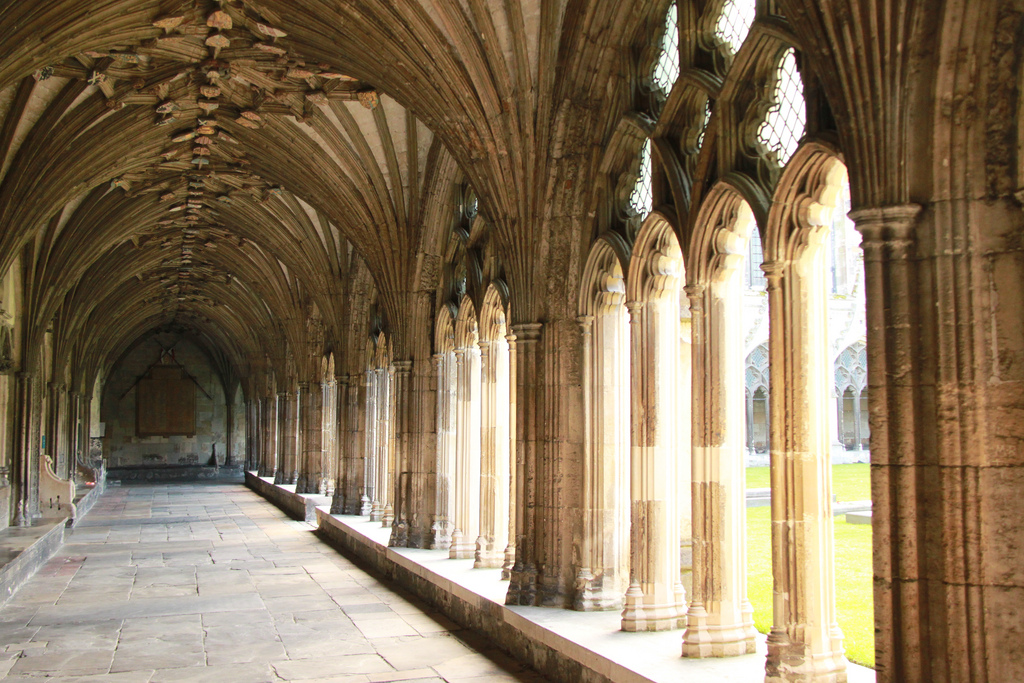
\includegraphics[width=0.95\textwidth]{/part03/canterbury_cathedral.jpg}
 \begin{center}
 {\large ``Canterbury Cathedral''}
 \par
 Foto di Bortescristian
 \par
 \url{http://www.flickr.com/photos/bortescristian/5083747705/}\par
 Licenza: Attribuzione 2.0 Generico (CC BY 2.0)\par
 \end{center}
\clearpage
\cleardoublepage
 
% (c)~2014 Claudio Carboncini - claudio.carboncini@gmail.com
% (c)~2014 Dimitrios Vrettos - d.vrettos@gmail.com
\chapter{Equazioni di grado superiore al secondo}
\section{L'equazione di terzo grado, un po' di storia}
Problema: ``Trovare un numero il cui cubo, insieme con due suoi quadrati e dieci volte il numero stesso, dia come somma 20''.

Il problema enunciato venne posto da Giovanni Panormita, astronomo e filosofo alla corte di Federico II, a Leonardo Pisano, detto Fibonacci, che ne tentò la soluzione nella sua opera ``Flos''.

Con il linguaggio matematico attuale il problema si formalizza nell'equazione di terzo grado $x^3+2x^2+10x=20$; Fibonacci pervenne al valore approssimato $x=\np{1,3688}$ come soluzione al problema, senza indicare la via seguita per la sua determinazione. Pur tuttavia egli riuscì a dimostrare che le soluzioni di un'equazione di terzo grado non possono mai esprimersi mediante radicali quadratici neanche se sovrapposti.

Solo tra il 1540 e il 1545, ad opera dei matematici italiani Niccolò Fontana, detto Tartaglia\footnote{soprannome dovuto al suo linguaggio balbettante (1499 ca. - 1557).}, e Gerolamo Cardano\footnote{matematico, medico, astrologo e filosofo (1501 - 1576).}, fu scoperta la formula risolutiva dell'equazione generale di terzo grado.
Cardano dimostrò che ogni equazione di terzo grado $ax^3+bx^2+cx+d=0$ è riconducibile alla forma $y^3+py+q=0$ operando la sostituzione $x=y-\frac b{3a}$, per la quale si ricava la formula risolutiva: 
\[y=\sqrt[3]{-\frac q 2+\sqrt{\left(\frac p 3\right)^3+\left(\frac q 2\right)^2}}+\sqrt[3]{-\frac q 2-\sqrt{\left(\frac p 3\right)^3+\left(\frac q 2\right)^2}}\] 
da cui poi si risale alla soluzione in $x$ dell'equazione assegnata.
\begin{exrig}
\begin{esempio}
Risolvere l'equazione: $x^3+3x^2+6x+5=0$.

Operiamo la sostituzione $x=y-\frac b{3a}$ che in questo caso è $x=y-1$; l'equazione diventa $(y-1)^3+3(y-1)^2+6(y-1)+5=0$ ed eseguendo i calcoli si ha $y^3+3y+1=0$, quindi $p=3$ e $q=1$.
Applicando la formula risolutiva si ha 
\[y=\sqrt[3]{-\frac 1 2+\sqrt{\frac 1 4+1}}+\sqrt[3]{-\frac 1 2-\sqrt{\frac 1 4+1}}=\sqrt[3]{\frac{\sqrt 5-1} 2}+\sqrt[3]{\frac{-\sqrt 5-1} 2}\] 
e quindi, sostituendo $y=x+1$, si ha $x=\sqrt[3]{\dfrac{\sqrt 5-1} 2}+\sqrt[3]{\dfrac{-\sqrt 5-1} 2}-1$.
\end{esempio}

\begin{esempio}
Risolvere l'equazione $x^3=15x+4$ applicando la formula di Cardano.

Notiamo che è $p=-15$ e $q=-4$ e dunque sotto la radice quadrata della formula 
si ha $\left(\frac p 3\right)^3+\left(\frac q 2\right)^2=(-5)^3+(-2)^2=-121$ pertanto non un numero
reale, mentre è evidente la soluzione reale $x=4$, infatti $4^3=64=15\cdot 4+4$. Questa circostanza ha spinto il matematico Raffaele Bombelli\footnote{matematico ed ingegnere italiano, noto anche con il nome di Rafael o Raphael (1526 - 1572).}, ad elaborare nella sua opera ``Algebra'' del 1572, calcoli con radici quadrate di numeri negativi (numeri) che troveranno una sistemazione coerente nella teoria dei \emph{numeri complessi} sviluppata da Friedrich Gauss.\footnote{Johann Carl Friedrich Gauss è stato un matematico, astronomo e fisico tedesco (1777 - 1855).}

Vediamo come possiamo determinare l'$IS$ dell'equazione di Bombelli con le nostre conoscenze. Scriviamo l'equazione nella forma canonica $p(x)=0\:\Rightarrow\: x^3-15x-4=0$; sappiamo che uno zero intero è $x=4$ dunque scomponiamo dividendo $p(x)=x^3-15x-4$ per il binomio $x-4$. Potete verificare che si ottiene $x^3-15x-4=(x-4)\cdot (x^2+4x+1)=0$ da cui, per la legge di annullamento del prodotto, 
\[x-4=0\:\Rightarrow\: x=4\quad\vee\quad x^2+4x+1=0\:\Rightarrow\: x_{1\text{,}2}=-2\pm \sqrt 3.\]

Poco dopo la scoperta della formula risolutiva per le equazioni di terzo grado, il matematico italiano Ferrari\footnote{Lodovico Ferrari (1522 - 1565).} trovò anche la formula per risolvere le equazioni di quarto grado. Le ricerche per trovare la formula che risolvesse l'equazione di quinto grado furono invece vane, non perché i matematici non furono abbastanza ``ingegnosi'' bensì per il fatto che, come dimostrò Galois\footnote{\'{E}variste Galois è stato un matematico francese (1811 - 1832).} non esistono formule che per mezzo di radici ed altre operazioni algebriche possano risolvere le 
equazioni dal quinto grado in poi. In altre parole, esistono solo formule per le equazioni di primo, secondo, terzo e quarto grado.

Oggigiorno, tuttavia, si preferisce non approfondire le applicazioni di queste formule. Lo studio è generalmente rivolto soltanto alle equazioni di primo e secondo grado e per quelle di grado superiore al secondo si applicano i metodi che vedremo in questo capitolo, oppure si utilizzano metodi di calcolo numerico che forniscono soluzioni per approssimazioni successive.
\end{esempio}
\end{exrig}

\section{Equazioni riconducibili al prodotto di due o più fattori}

In questo capitolo ci proponiamo di determinare l'insieme soluzione di equazioni algebriche di grado superiore al secondo.

Ricordiamo che un'equazione algebrica si presenta nella forma $p(x)=0$ dove $p(x)$ è un polinomio nella variabile $x$, di grado $n$, a coefficienti reali: \[a_nx^n+a_{n-1}x^{n-1}+ \ldots +a_2x^2+a_1x+a_0=0.\]

\begin{exrig}
\begin{esempio}
Determinare le radici reali dell'equazione $4x^3+x^2-4x-1=0$.

Scomponiamo in fattori il polinomio al primo membro mediante raccoglimento parziale: 
\[p(x)=4x^3+x^2-4x-1=4x \left(x^2-1\right)+\left(x^2-1\right)=\left(x^2-1\right) (4x+1).\] 
Per la legge dell'annullamento del prodotto si ottiene 
\[x^2-1=0 \quad\Rightarrow\quad x_1=-1 \;\vee\;x_2=1\text{,}\]
\[4x+1=0 \quad\Rightarrow\quad x=-\frac{1}{4}.\]
L'equazione ha dunque tre soluzioni reali distinte e $\IS=\left\{-1\text{, }1\text{, }-\frac 1 4\right\}$.
\end{esempio}
\begin{esempio}
Determinare le radici reali dell'equazione fratta $\dfrac{2x+3}{2x+1}+\dfrac{x^2}{x+1}=5x+3$.

Riduciamo allo stesso denominatore 
\[\frac{2x^2+5x+3+2x^3+x^2-10x^3-15x^2-5x-6x^2-9x-3}{(2x+1)\cdot (x+1)}=0.\]
Poniamo le condizioni d'esistenza: $x\neq -\frac 1 2\wedge x\neq -1$. Eliminiamo il denominatore e sommiamo i monomi simili; otteniamo un'equazione di terzo grado $8x^3+18x^2+9x=0$, che, scomponendo il polinomio, può essere scritta come $x\cdot \left(8x^2+18x+9\right)=0$. Per la legge di annullamento del prodotto si ha $x=0\;\vee\;x^2+18x+9=0$. Risolvendo anche l'equazione di secondo grado con la formula risolutiva si ottengono le soluzioni $x_1=0\;\vee\; x_2=-\frac 3 4\;\vee\; x_3=-\frac 3 2$.

\osservazione
Si dimostra che un'equazione ammette tante soluzioni, che possono essere reali (distinte o coincidenti) o non reali, quante ne indica il suo grado.

Ricordiamo che uno zero di un polinomio è il valore che assegnato alla variabile rende il polinomio uguale a zero. Quindi trovare gli zeri di un polinomio equivale a trovare le soluzioni dell'equazione che si ottiene ponendo il polinomio uguale a zero, come nell'esempio seguente.
\end{esempio}

\begin{esempio}
Trovare gli zeri del seguente polinomio di terzo grado $p(x)=x^3-7x^2+4x+12$.

Scriviamo l'equazione $x^3-7x^2+4x+12=0$ e cerchiamo di scomporre con il metodo di Ruffini. Sostituendo $x=-1$ si ottiene $(-1)^3-7(-1)^2+4(-1)+12=-1-7-4+12=0$. Possiamo allora dividere il polinomio $p(x)$ per il binomio $x+1$. Applicando la regola di Ruffini si ha:
\begin{center}
% (c) 2013 Claudio Carboncini - claudio.carboncini@gmail.com

\begin{tikzpicture}[x=5mm,y=5mm]
\matrix (a)[matrix of nodes, nodes in empty cells,nodes={ text width=8mm, text depth=1mm, text centered}]{
&$1$&$-7$&$4$&$ 12 $\\
$ -1 $&&$ -1 $&$ 8 $&$-12$\\
&$ 1 $&$ -8 $&$12$&//\\
};  
\begin{scope}[blue]
\draw(a-1-2.north west)--(a-3-1.south east);
\draw(a-2-1.south west)--(a-2-5.south east);
\draw(a-1-4.north east)--(a-3-4.south east);
      \end{scope}
\end{tikzpicture}

\end{center}
Il polinomio si scompone in $(x+1)(x^2-8x+12)$. Per la legge di annullamento del prodotto $x+1=0\;\vee\; x^2-8x+12=0$. L'equazione $x+1=0$ dà come soluzione $x=-1$. L'equazione $x^2-8x+12=0$ si può risolvere con la formula risolutiva ridotta $x_{1\text{,}2}=4\pm \sqrt{16-12}=4\pm 2$. Il polinomio assegnato ha tre zeri distinti $x_1=-1\;\vee\; x_2=2\;\vee\; x_3=6$.
\end{esempio}
\end{exrig}
\ovalbox{\risolvii \ref{ese:5.1}, \ref{ese:5.2}, \ref{ese:5.3}, \ref{ese:5.4}, \ref{ese:5.5}, \ref{ese:5.6}, \ref{ese:5.7}, \ref{ese:5.8}, \ref{ese:5.9}, \ref{ese:5.10}, \ref{ese:5.11}}

\section{Equazioni binomie}

\begin{definizione}
Un'\emph{equazione binomia} è un'equazione del tipo $ax^n+b=0$ con $a\neq 0$ e con $n\in \insN_0$.
\end{definizione}

L'equazione scritta come $ax^n+b=0$ è detta in \emph{forma normale} o \emph{canonica}.

Dobbiamo distinguere i casi:
\begin{itemize*}
\item $n$ è pari e $ a\cdot b< 0 $. I coefficienti $ a $ e $ b $ hanno segno discorde. L'equazione ammette due sole soluzioni reali ed opposte: $x_1=\sqrt[n]{-\frac b a}\;\vee\; x_2=-\sqrt[n]{-\frac b a}$;
\item $n$ è pari e $ a\cdot b> 0 $. I coefficienti $ a $ e $ b $ hanno lo stesso segno. L'equazione non ammette soluzioni reali;
\item $n$ è dispari e $ b\neq 0 $. L'equazione ha un'unica soluzione reale $x_1=\sqrt[n]{-\frac b a}$;
\item $b=0$. L'equazione è $ax^n=0$ e le $n$ soluzioni sono coincidenti nell'unica soluzione $x=0$. In questo caso si dice che l'unica soluzione $x=0$ ha molteplicità $n$.
\end{itemize*}
%\newpage
\begin{exrig}
 \begin{esempio}
Risolvere le seguenti equazioni binomie
\begin{itemize}
\item $3x^4-8=0$.

L'esponente $n$ è pari, i coefficienti sono discordi: l'equazione ammette due soluzioni reali distinte: $x_1=\sqrt[4]{\frac 8 3}\;\vee\; x_2=-\sqrt[4]{\frac 8 3}$.

Osserviamo che l'equazione proposta può essere risolta col metodo della scomposizione in fattori: $3x^4-8=0 \:\Rightarrow\: \left(\sqrt 3x^2+\sqrt 8\right)\cdot \left(\sqrt 3x^2-\sqrt 8\right)=0$ e per la legge di annullamento del prodotto $\left(\sqrt 3x^2+\sqrt 8\right)=0\;\vee\; \left(\sqrt 3x^2-\sqrt 8\right)=0$. La prima equazione non ha soluzioni reali, mentre per la seconda si ha $x^2=\sqrt{\frac 8 3}\:\Rightarrow\: x=\pm \sqrt{\sqrt{\frac 8 3}}\:\Rightarrow\: x=\pm \sqrt[4]{\frac 8 3}$.

\item $-6x^4+9=13$.

Riducendo alla forma normale troviamo $-6x^4-4=0$; moltiplicando ambo i membri per $-1$ si ottiene $6x^4+4=0$ in cui il primo membro è una somma di numeri sempre positivi sempre maggiore di zero, quindi in $\insR$ l'equazione è impossibile e $\IS=\emptyset $.

\item $8x^3+3=4$.

Riduciamo l'equazione alla forma normale $8x^3-1=0$. Essendo di grado dispari, l'unica soluzione è $x=\sqrt[3]{\frac 1 8}=\frac 1 2$.

Allo stesso risultato perveniamo scomponendo in fattori la differenza di due cubi: $8x^3-1=0 \:\Rightarrow\: (2x-1)\cdot \left(4x^2+2x+1\right)=0$. Per la legge di annullamento del prodotto $2x-1=0 \:\Rightarrow\: x=\frac 1 2\ \:\vee\: \ 4x^2+2x+1=0$ ma l'equazione di secondo grado non ha soluzioni reali essendo $\Delta <0$. Pertanto l'unica soluzione è $x=\frac 1 2$, quindi $\IS=\left\{\frac 1 2\right\}$.

\item $ 2x^7+3=2 $.

In forma normale $2x^7+1=0$. Si trova così l'unica soluzione reale $x=\sqrt[7]{-\frac 1 2}=-\sqrt[7]{\frac 1 2}$.

\item $3x\cdot \left(x^4-1\right)=4\cdot (1+x)-(7x+4)$.

Sviluppando i calcoli si ottiene $3x^5=0 \:\Rightarrow\: x^5=0 \:\Rightarrow\: x=0$, cioè una sola soluzione reale con molteplicità $5$.

\item $x^3+3=0$.

L'equazione ha l'unica soluzione reale $x=-\sqrt[3]3$. Spieghiamo il risultato scomponendo la somma di cubi $\left(x\right)^3+\left(\sqrt[3]3\right)^3=0 \:\Rightarrow\: \left(x+\sqrt[3]3\right) \left(x^2-x\sqrt[3]3+\sqrt[3]{3^2}\right)=0$. Per la legge di annullamento del prodotto otteniamo: $\left(x+\sqrt[3]3\right)=0 \:\Rightarrow\: x=-\sqrt[3] 3$ e $x^2-\sqrt[3]3 x+\sqrt[3]{3^2}=0$ che non ha soluzioni reali essendo $\Delta <0$.
\end{itemize}
 \end{esempio}
\end{exrig}

\ovalbox{\risolvii \ref{ese:5.12}, \ref{ese:5.13}, \ref{ese:5.14}, \ref{ese:5.15}, \ref{ese:5.16}, \ref{ese:5.17}, \ref{ese:5.18}, \ref{ese:5.19}, \ref{ese:5.20}}

\section{Equazioni trinomie}

\begin{definizione}
Un'\emph{equazione trinomia} è un'equazione del tipo $ax^{2n}+bx^n+c=0$ dove $n \in \insN_0$~~e~~$a\neq 0$,~~$b\neq 0$.
\end{definizione}

Sono esempi di equazioni trinomie $x^4-5x^2+4=0$,\ \  $x^6-4x^3+3=0$,\ \ $x^{10}-x^5+6=0$.

Per risolvere queste equazioni è opportuno fare un cambio di incognita: ponendo $t=x^n$ l'equazione trinomia diventa di secondo grado: $at^2+bt+c=0$ e da questa, detta \emph{equazione risolvente}, si ricavano i valori di $t$. Successivamente, dalla relazione $t=x^n$, si ricavano i valori di $x$.

\subsection{Equazione biquadratica}

Se $n=2$ l'equazione è detta \emph{biquadratica} e si presenta nella forma~~$ax^4+bx^2+c=0$.

\begin{exrig}
\begin{esempio}
Risolvere le seguenti equazioni biquadratiche.
\begin{itemize}
\item $ x^4-5x^2+4=0 $.

L'equazione è biquadratica; facciamo un cambio di incognita ponendo $x^2=t$; l'equazione diventa $t^2-5t+4=0$ che ha due soluzioni reali distinte $t_1=1\;\vee \;t_2=4$. Per determinare le soluzioni dell'equazione assegnata teniamo conto della sostituzione fatta. Da $t_1=1$ otteniamo $x^2=1$ con soluzioni $x_1=-1\;\vee\; x_2=+1$ e da $t_2=4$ otteniamo $x^2=4$ con soluzioni $x_1=-2\;\vee\; x_2=+2$. Pertanto l'equazione assegnata ha quattro soluzioni reali distinte e $\IS=\{-1\text{, }+1\text{, }-2\text{, }+2\}$.

\item $ 2x^4+3x^2-2=0 $.

L'equazione è biquadratica, ponendo $x^2=t$ diventa $2t^2+3t-2=0$ che ha per soluzioni $t_1=-2\;\vee\; t_2=\frac 1 2$. Ritornando alla sostituzione iniziale, da $t_1=-2$ otteniamo $x^2=-2\:\Rightarrow\: \IS=\emptyset $ e da $t_2=\frac 1 2$ otteniamo $x^2=\frac 1 2$ con soluzioni $x_1=-\sqrt{\frac 1 2}\;\vee\; x_2=+\sqrt{\frac 1 2}$ e razionalizzando $x_1=-\frac{\sqrt 2} 2\;\vee\; x_2=+\frac{\sqrt 2} 2$.

\item $ x^4-\frac{16} 9x^2=0 $.

L'equazione è biquadratica incompleta; si può determinare l'insieme soluzione raccogliendo $x^2$ a fattore comune, ottenendo così $x^2\left(x^2-\frac{16} 9\right)=0$ e per la legge di annullamento del prodotto possiamo concludere $x^2=0\;\vee\; x^2=\frac{16} 9$ da cui $\IS=\left\{0\text{, }-\frac 4 3\text{, }+\frac 4 3\right\}$.
 \end{itemize}

\end{esempio}
\end{exrig}
\conclusione
L'equazione biquadratica ${ax}^4+{bx}^2+c=0$
\begin{itemize*}
\item ha quattro soluzioni reali distinte se il discriminante dell'equazione risolvente è positivo e se risultano positivi anche i rapporti $-\frac b a$ e $\frac c a$ che indicano rispettivamente la somma e il prodotto delle sue soluzioni. Infatti \dotfill;
\item ha due soluzioni reali distinte se il discriminante dell'equazione risolvente è positivo e se risulta negativo il rapporto $\frac c a$ che indica il prodotto delle sue soluzioni. Infatti \dotfill;
\item non ha soluzioni reali se il discriminante dell'equazione risolvente è positivo e se risulta positivo il rapporto $\frac c a$ e negativo il rapporto $-\frac b a$. Infatti \dotfill;
\item non ha soluzioni reali se il discriminante dell'equazione risolvente è negativo.
\end{itemize*}
Per stabilire il numero di soluzioni di un'equazione biquadratica si può anche utilizzare la regola dei segni di Cartesio:
\begin{itemize*}
\item $\Delta >0$ e due variazioni si hanno 4 soluzioni reali;
\item $\Delta >0$ una permanenza e una variazione si hanno 2 soluzioni reali;
\item $\Delta =0$ e~~~$-\frac b{2a}>0$ si hanno due soluzioni reali; $-\frac b{2a}<0$ nessuna soluzione reale;
\item $\Delta <0$ nessuna soluzione reale.
\end{itemize*}

\ovalbox{\risolvii \ref{ese:5.21}, \ref{ese:5.22}, \ref{ese:5.23}, \ref{ese:5.24}, \ref{ese:5.25}, \ref{ese:5.26}, \ref{ese:5.27}, \ref{ese:5.28}, \ref{ese:5.29}, \ref{ese:5.30}, \ref{ese:5.31}}

\subsection{Equazioni trinomie con n maggiore di 2}

\begin{exrig}
\begin{esempio}
Risolvere le seguenti equazioni trinomie.
\begin{itemize}
\item $ x^6-4x^3+3=0 $.

Ponendo $t=x^3$ abbiamo l'equazione risolvente $t^2-4t+3=0$, le cui soluzioni reali sono $t_1=1$, $t_2=3$; per ricavare i valori di $x$ è sufficiente risolvere le due equazioni binomie $x^3=1$ e $x^3=3$, trovando così le soluzioni reali per l'equazione assegnata $x_1=1\;\vee\; x_2=\sqrt[3]3$;

\item $ x^8-x^4-2=0 $.

Ponendo $t=x^4$ arriviamo all'equazione $t^2-t-2=0$ da cui $t_1=2$ e $t_2=-1$; pertanto le due equazioni binomie da risolvere sono: $x^4=2$ e $x^4=-1$. Quindi $x^4=2\:\Rightarrow\: x^2=-\sqrt 2\;\vee\; x^2=\sqrt 2$ e di queste due, solo la seconda ha soluzioni reali e precisamente $x_1=\sqrt[4]2 \;\vee\; x_2=-\sqrt[4]2$; la prima equazione binomia $x^4=-1$ non ha invece soluzioni reali. Concludendo: $\IS=\left\{-\sqrt[4]2\text{, }\sqrt[4]2\right\}$.
\end{itemize}
\end{esempio}
\end{exrig}
\ovalbox{\risolvii \ref{ese:5.32}, \ref{ese:5.33}}

\section{Equazioni che si risolvono con sostituzioni}

Molte altre equazioni si possono risolvere con opportune sostituzioni.
\begin{exrig}
\begin{esempio}
Risolvere la seguente equazione $ \left(x^2-4\right)^4-1=0 $.

Sostituendo $t=x^2-4$ l'equazione diventa $t^4-1=0$. È un'equazione binomia che ha per soluzioni $t_1=-1$, $t_2=+1$. Sostituendo questi valori nella relazione $t=x^2-4$ si ha: 
\[x^2-4=-1\:\Rightarrow\: x^2=3\:\Rightarrow\: x_{1\text{,}2}=\pm \sqrt 3\quad\text{ e }\quad x^2-4=+1\:\Rightarrow\: x^2=5\:\Rightarrow\: x_{3\text{,}4}=\pm \sqrt 5.\]
\end{esempio}
\end{exrig}
\ovalbox{\risolvii \ref{ese:5.34}, \ref{ese:5.35}, \ref{ese:5.36}, \ref{ese:5.37}}

\section{Equazioni reciproche}

\begin{definizione}
Un'equazione è detta \emph{reciproca di prima specie} se, posta nella forma canonica $p(x)=0$, il polinomio $p(x)$ ha i coefficienti dei termini estremi e quelli dei termini equidistanti dagli estremi \emph{uguali}.
\end{definizione}

\begin{definizione}
Un'equazione è detta \emph{reciproca di seconda specie} se, posta nella forma canonica $p(x)=0$, il polinomio $p(x)$ ha i coefficienti dei termini estremi e quelli dei termini equidistanti dagli estremi \emph{opposti}. In particolare, se $p(x)$ ha grado $2k$ (pari), il coefficiente di $x^k$ è nullo.
\end{definizione}

Dalle definizioni si ha che:

\begin{itemize*}
\item $x^3-2x^2-2x+1=0$ è un'equazione di terzo grado reciproca di prima specie;
\item $3x^4+5x^3-4x^2+5x+3=0$ è un'equazione di quarto grado reciproca di prima specie;
\item $-7x^4+5x^3-5x+7=0$ è un'equazione di quarto grado reciproca di seconda specie;
\item $3x^5+2x^4+6x^3-6x^2-2x-3=0$ è un'equazione di quinto grado reciproca di seconda specie;
\item $-2x^4+8x^3+3x^2-8x+2=0$ è un'equazione di quarto grado, ma non è reciproca di seconda specie, in quanto il coefficiente di secondo grado dovrebbe essere nullo.
\end{itemize*}

Il seguente teorema mette in luce una importante proprietà di cui godono queste equazioni.
\begin{teorema}[delle radici reciproche]
Se $\lambda$ è una radice non nulla di un'equazione reciproca di qualunque grado, allora anche $\dfrac 1{\lambda}$ è radice dell'equazione.
\end{teorema}

Consideriamo il polinomio dell'equazione reciproca di prima specie
\[p(x)=a_0x^n+a_1x^{n-1}+a_2x^{n-2}+ \ldots +a_2x^2+a_1x+a_0.\]

\emph{Ipotesi}. $x=\lambda$ è una radice dell'equazione $p(x)=0$;

\emph{Tesi}. $x=\frac 1{\lambda}$ è una radice dell'equazione $p(x)=0$.
\begin{proof}
Sappiamo che se $x=\lambda$ è una radice di $p(x)=0$ allora $p(\lambda)=0$, cioè
\[p(\lambda)=a_0\lambda ^n+a_1\lambda ^{n-1}+\ldots +a_1\lambda +a_0=0.\]

Scriviamo il polinomio con $x=\frac 1{\lambda }$
\begin{align*}
p\left(\frac 1{\lambda }\right)&=a_0\left(\frac 1{\lambda }\right)^n+a_1\left(\frac 1{\lambda }\right)^{n-1}+\ldots +a_1\left(\frac 1{\lambda }\right)+a_0\\
&=\frac 1{\lambda ^n} \left(a_0+a_1\lambda +\ldots +a_1\lambda ^{n-1}+a_0\lambda ^n \right)\\
\end{align*}
dove nell'ultimo passaggio abbiamo messo in evidenza il termine $ \left(\frac 1{\lambda }\right)^n $ (è consentito perché per ipotesi $\lambda$ non è nullo). Confrontando le scritture di $p(\lambda)$ e $p\left(\frac 1{\lambda }\right)$ risulta
\[
p\left(\frac 1{\lambda }\right)=\frac 1{\lambda ^n} p(\lambda)=0
\]
Quindi anche $\dfrac 1{\lambda }$ è una radice di $p(x)=0$.
\end{proof}
Dimostra tu il teorema per le equazioni di seconda specie.

\subsection{Equazioni di terzo grado reciproche di prima specie}

Queste equazioni hanno la seguente struttura: \[a_0x^3+a_1x^2+a_1x+a_0=0.\]
Una radice dell'equazione è $x=-1$, infatti sostituendo tale valore al posto della $x$ nel polinomio al primo membro si ottiene: \[p(-1)=a_0(-1)^3+a_1(-1)^2+a_1(-1)+a_0=-a_0+a_1-a_1+a_0=0.\]

Ricordiamo che secondo la regola del resto, il valore trovato (zero) ci assicura che il polinomio al primo membro è divisibile per $x+1$; con la divisione polinomiale o con la regola di Ruffini possiamo scrivere $a_0x^3+a_1x^2+a_1x+a_0=(x+1)\cdot \left(a_0x^2+(a_1-a_0)x+a_0\right)=0$ da cui, per la legge di annullamento del prodotto, possiamo determinare le soluzioni dell'equazione assegnata.

Un modo alternativo per determinare l'insieme soluzione dell'equazione reciproca di prima specie consiste nel raccogliere parzialmente i due coefficienti $a_0$ e $a_1$ in modo da ottenere $a_0\left(x^3+1\right)+a_1\left(x^2+x\right)=0$ da cui $a_0(x+1)\left(x^2-x+1\right)+a_1x(x+1)=0$ e raccogliendo il binomio $(x+1)$ ritroviamo la fattorizzazione precedente: $(x+1) \left(a_0x^2+(a_1-a_0)x+a_0\right)=0$.
\begin{exrig}
 \begin{esempio}
 Risolvere le seguenti equazioni di terzo grado reciproche di prima specie.

 \begin{itemize}
 \item $x^3-5x^2-5x+1=0$.

 Si tratta di un'equazione di terzo grado reciproca di prima specie. Una radice è $x=-1$, per cui possiamo fattorizzare il polinomio al primo membro eseguendo la divisione polinomiale e ottenere $(x+1)\left(x^2-6x+1\right)=0$. Per la legge di annullamento del prodotto otteniamo la radice $x=-1$ già nota e, risolvendo l'equazione $x^2-6x+1=0$ troviamo le altre radici $x_2=3+2\sqrt 2$~~e~~$x_3=3-2\sqrt 2$. Quindi $\IS=\left\{-1\text{, }3+2\sqrt 2\text{, }3-2\sqrt 2\right\}$.

 Notiamo che $x_2$ e $x_3$ sono tra loro reciproche: $x_2 \cdot x_3=1$ cioè $(3+2\sqrt 2)\cdot (3-2\sqrt 2)=1$.

 \item $3x^3-5x^2-5x+3=0$

 L'equazione assegnata è reciproca di terzo grado e di prima specie; ammette dunque $x=-1$ come radice. Infatti $p(-1)=3(-1)^3-5(-1)^2-5(-1)+3=\ldots$ Il polinomio al primo membro si può scomporre con la regola di Ruffini cioè $(x+1)\left(3x^2-8x+3\right)=0$; per la legge di annullamento del prodotto avremo $x+1=0\:\Rightarrow\: x=-1$, come già noto, e $3x^2-8x+3=0$ con soluzioni $x_2=\ldots $ e $x_3=\ldots$ Quindi $\IS=\{\dotfill \}$.
 \end{itemize}
 \end{esempio}
\end{exrig}
\ovalbox{\risolvii \ref{ese:5.38}, \ref{ese:5.39}, \ref{ese:5.40}, \ref{ese:5.41}}

\subsection{Equazioni di terzo grado reciproche di seconda specie}

Queste equazioni hanno la seguente struttura:
\[a_0x^3+a_1x^2-a_1x-a_0=0.\]
Una radice dell'equazione è $x=1$, basta verificare sostituendo tale valore al posto della $x$ nel polinomio al primo membro. Si ottiene: \[p(1)=a_0(1)^3+a_1(1)^2-a_1(1)-a_0=a_0+a_1-a_1-a_0=0.\]

Procedendo come nel caso precedente si può ottenere la scomposizione in fattori del polinomio al primo membro: $(x-1)\cdot \left(a_0x^2+(a_0+a_1)x+a_0\right)=0$ e quindi determinare l'$\IS$ dell'equazione assegnata applicando la legge di annullamento del prodotto.
\begin{exrig}
 \begin{esempio}
 Risolvere le seguenti equazioni di terzo grado reciproche di seconda specie

 \begin{itemize}
 \item $ 2x^3-7x^2+7x-2=0 $.

 \`E un'equazione di terzo grado reciproca di seconda specie, i coefficienti infatti sono opposti a due a due. Una radice è $x_1=1$ infatti $p(1)=2-7+7-2=0$. Applicando la regola di Ruffini per scomporre il polinomio di terzo grado si ottiene $(x-1)\left(2x^2-5x+2\right)=0$. Per la legge di annullamento del prodotto abbiamo la radice $x=1$, già nota, e risolvendo $\left(2x^2-5x+2\right)=0$ si ricavano le altre due radici: $x_2=2$~~e~~$x_3=\frac 1 2$. Dunque $\IS=\left\{1\text{, }2\text{, }\frac 1 2\right\}$.

 \item $ 2x^3-9x^2+9x-2=0 $.

 L'equazione assegnata è reciproca di terzo grado e di seconda specie perché ha i coefficienti opposti a due a due, quindi ammette $x=+1$ come radice. Infatti $p(1)=\ldots$
 Applichiamo la regola di Ruffini per scomporre in fattori il polinomio di terzo grado. Il polinomio si scompone in $(x-1)\left(2x^2- \ldots \ldots\right)=0$. Per la legge di annullamento del prodotto avremo $x-1=0\:\Rightarrow\: x=1$, come già noto, e $2x^2-7x+2=0$ con soluzioni $x_2=\ldots $ e $x_3=\ldots $. Quindi $\IS=\{\ldots \ldots \ldots \}$. L'equazione assegnata ha tre soluzioni reali di cui le due irrazionali sono l'una il reciproco dell'altra.
 \end{itemize}
 \end{esempio}
\end{exrig}
\ovalbox{\risolvii \ref{ese:5.42}, \ref{ese:5.43}, \ref{ese:5.44}}

\subsection{Equazioni di quarto grado reciproche di prima specie}

Rientrano in questa classificazione le equazioni del tipo: \[a_0x^4+a_1x^3+a_2x^2+a_1x+a_0=0.\]

Prima di tutto osserviamo che $x=0$ non può essere una radice in quanto, se lo fosse, sarebbe nullo il termine noto, cioè $a_0=0$ e di conseguenza sarebbe nullo anche il coefficiente di $x^{4}$ quindi il grado dell'equazione diventerebbe 3 o inferiore. Questa premessa ci consente di dividere per $x^2$ ottenendo l'equazione equivalente $a_0 x^2+a_1x+a_2+\dfrac{a_1} x+\dfrac{a_0}{x^2}=0$ e raccogliendo a fattori parziali si ha $a_0\left(x^2+\dfrac 1{x^2}\right)+a_1\left(x+\dfrac 1 x\right)+a_2=0$.

Ponendo~~$t=x+\dfrac 1 x$~~si ha~~$t^2=\left(x+\dfrac 1 x\right)^2\:\Rightarrow\: t^2=x^2+\dfrac 1{x^2}+2 \:\Rightarrow\: x^2+\dfrac 1{x^2}=t^2-2$.

Sostituendo nell'equazione otteniamo la seguente equazione di secondo grado equivalente a quella data: $a_0\left(t^2-2\right)+a_1t+a_2=0$, ovvero
\[a_0t^2+a_1t+a_2-2a_0=0.\]

Una volta trovate, se esistono (reali), le radici $t_1$ e $t_2$ di questa equazione, possiamo determinare le corrispondenti radici dell'equazione iniziale risolvendo le due equazioni fratte $x+\dfrac 1 x=t_1$~~e~~$x+\dfrac 1 x=t_2$~~nell'incognita $x$, rispettivamente equivalenti a
\[x^2-t_1x+1=0\qquad\text{e}\qquad {x}^2-t_2x+1=0.\]

Queste ultime equazioni hanno soluzioni reali se e solo se $|t|\ge 2$. Infatti, risolvendo rispetto a $x$ l'equazione $x+\dfrac 1 x=t$, troviamo: $x^2-tx+1=0$ e calcolando il discriminante $\Delta =t^2-4$ vediamo che ci sono soluzioni reali se e solo se $t^2-4\ge 0$ ovvero se e solo se $t\le -2 \;\vee\; t\ge 2$ cioè $|t|\ge 2$.
%\newpage
\begin{exrig}
 \begin{esempio}
 Risolvere le seguenti equazioni di quarto grado reciproche di prima specie.
 \begin{itemize}
 \item $x^4-4x^3+5x^2-4x+1=0$.

 Si tratta di un'equazione di quarto grado reciproca di prima specie. Dividiamo per $x^2$, otteniamo $x^2-4x+5-4\frac 1 x+\frac 1{x^2}=0$. Raccogliendo in fattori comuni come nella regola abbiamo $\left(x^2+\frac 1{x^2}\right)-4\left(x+\frac 1 x\right)+5=0$. Ponendo $t=x+\frac 1 x$ otteniamo l'equazione $ \left(t^2-2\right)-4t+5=0$ ovvero $t^2-4t+3=0$ da cui $t_1=1$ e $t_2=3$. Il primo valore $t_1$ non dà soluzioni reali poiché l'equazione $x+\frac 1 x=1$ ha il discriminante negativo mentre l'equazione $x+\frac 1 x=3$ ha due soluzioni reali distinte $x_1=\frac{3+\sqrt 5} 2$ e $x_2=\frac{3-\sqrt 5} 2$.

 \item $ 2x^4+3x^3-16x^2+3x+2=0 $.

 Dividiamo ambo i membri dell'equazione per $x^2$, certamente diverso da zero e otteniamo: $2x^2+3x-16+3\cdot \frac 1 x+2\cdot \frac 1{x^2}=0$. Mettiamo in evidenza $ 2 $ nel primo e quinto addendo e $ 3 $ tra il secondo e quarto addendo: $2\cdot \left(x^2+\frac 1{x^2}\right)+3\cdot \left(x+\frac 1 x\right)-16=0$. Ponendo $x+\frac 1 x=t$ otteniamo l'equazione $2(t^2-2)+3t-16=0\Rightarrow 2t^2+3t-20=0$ che ha come soluzioni $t_1=-4\vee t_2=\frac 5 2$. Poiché $|t|\ge 2$ le equazioni $x+\frac 1 x=t_1$ e $x+\frac 1 x=t_2$ hanno entrambe soluzioni reali distinte, pertanto $\IS=\left\{-2\sqrt{3}\text{, }2\sqrt{3}\text{, }\frac 1 2\text{, }2\right\}$.
 \end{itemize}
 \end{esempio}
\end{exrig}
\ovalbox{\risolvii \ref{ese:5.45}, \ref{ese:5.46}}

\subsection{Equazioni di quarto grado reciproche di seconda specie}

Fanno parte di questa classe le equazioni del tipo: \[a_0x^4+a_1x^3-a_1x-a_0=0\] in cui il coefficiente di $x^2$ è nullo. Per risolvere questa equazione, raccogliamo a fattore parziale $a_0$ e $a_1$ ottenendo: $a_0\left(x^4-1\right)+a_1\left(x^3-x\right)=0 \:\Rightarrow\: a_0\left(x^2-1\right)\left(x^2+1\right)+a_1x\left(x^2-1\right)=0$.

Raccogliendo a fattore comune totale si ha:
\[\left(x^2-1\right)\left[a_0\left(x^2+1\right)+a_1x\right]=0\quad\Rightarrow \quad\left(x-1\right)\left(x+1\right)\left(a_0x^2+a_1x+a_0\right)=0.\]
Per la legge di annullamento del prodotto si hanno quindi le due radici $x_1=1$, $x_2=-1$ e le eventuali radici reali dell'equazione di secondo grado $a_0x^2+a_1x+a_0=0$.
\begin{exrig}
 \begin{esempio}
 Risolvere l'equazione $x^4-8x^3+8x-1=0$.

 Si tratta di un'equazione di quarto grado reciproca di seconda specie, si osservi che il coefficiente di secondo grado è nullo e che gli altri coefficienti sono a due a due opposti.
 Raccogliendo a fattore comune parziale abbiamo 
\[(x^4-1)-8x(x^2-1)=0\quad\Rightarrow\quad (x^2-1)(x^2+1)-8x(x^2-1)=0.\]
 Mettendo poi in evidenza il binomio $\left(x^2-1\right)$ abbiamo $\left(x^2-1\right)\left(x^2-8x+1\right)$. Risolvendo le equazioni $x^2-1=0$ e $x^2-8x+1=0$, otteniamo tutte le radici: 
\[x_1=1\;\vee\; x_2=-1\;\vee\; x_3=4+\sqrt{15}\;\vee\; x_4=4-\sqrt{15}\] 
e quindi 
\[\IS=\left\{-1\text{, }1\text{, }4+\sqrt{15}\text{, }4-\sqrt{15}\right\}.\]
 \end{esempio}
\end{exrig}
\ovalbox{\risolvii \ref{ese:5.47}, \ref{ese:5.48}, \ref{ese:5.49}, \ref{ese:5.50}, \ref{ese:5.51}}

\subsection{Equazioni di quinto grado reciproche di prima specie}

Fanno parte di questa classe le equazioni del tipo: \[a_0x^5+a_1x^4+a_2x^3+a_2x^2+a_1x+a_0=0.\]

Con il raccoglimento parziale otteniamo: 
\[a_0\left(x^5+1\right)+a_1\left(x^4+x\right)+a_2\left(x^3+x^2\right)=0.\]

Applichiamo ora la formula per la scomposizione della somma di potenze ottenendo
\[a_0(x+1)\left(x^4-x^3+x^2-x+1\right)+a_1x(x+1)\left(x^2-x+1\right)+a_2x^2(x+1)=0.\]
Raccogliendo $(x+1)$ ricaviamo: 
\[(x+1)\left[a_0\left(x^4-x^3+x^2-x+1\right)+a_1x\left(x^2-x+1\right)+a_2x^2\right]=0\]
e quindi l'equazione diventa:
\[(x+1)\left[a_0x^4+(a_1-a_0)x^3+(a_2-a_1+a_0)x^2+(a_1-a_0)x+a_0\right]=0.\]

Per la legge di annullamento del prodotto si determina la soluzione reale $x=-1$ e con i metodi analizzati in precedenza si risolve l'equazione di quarto grado reciproca di prima specie: 
\[\left(a_0x^4+(a_1-a_0)x^3+(a_2-a_1+a_0)x^2+(a_1-a_0)x+a_0\right)=0.\]
\pagebreak
\begin{exrig}
 \begin{esempio}
 Risolvere l'equazione $6x^5+x^4-43x^3-43x^2+x+6=0$.

 L'equazione è di quinto grado reciproca di prima specie. Una radice è $x_1=-1$ e l'equazione può essere scritta come: 
\[(x+1)\left(6x^4-5x^3-38x^2-5x+6\right)=0.\]
 Risolvendo l'equazione di quarto grado reciproca di prima specie 
\[6x^4-5x^3-38x^2-5x+6=0\text{,}\] 
si trovano le altre quattro radici: 
\[x_2=-2\text{,}\quad x_3=-\frac 1 2\text{,}\quad x_4=3\text{,}\quad x_5=\frac{1}{3}\] quindi 
\[\IS=\left\{-1\text{, }-2\text{, }-\frac 1 2\text{, }3\text{, }\frac 1 3\right\}.\]
 \end{esempio}
\end{exrig}

\subsection{Equazioni di quinto grado reciproche di seconda specie}
Fanno parte di questa classe le equazioni del tipo:
\[a_0x^5+a_1x^4+a_2x^3-a_2x^2-a_1x-a_0=0.\]

Con il raccoglimento parziale si ottiene 
\[a_0\left(x^5-1\right)+a_1\left(x^4-x\right)+a_2\left(x^3-x^2\right)=0.\]

 Applichiamo ora la formula per la scomposizione della differenza di potenze ottenendo: 
\[a_0(x-1)\left(x^4+x^3+x^2+x+1\right)+a_1x(x-1)\left(x^2+x+1\right)+a_2x^2(x-1)=0.\] 
Raccogliendo il binomio $(x-1)$ si ottiene 
\[(x-1)\left[a_0\left(x^4+x^3+x^2+x+1\right)+a_1x\left(x^2+x+1\right)+a_2x^2\right]=0\] e quindi 
\[(x+1)\left[a_0x^4+(a_1-a_0)x^3+(a_2-a_1+a_0)x^2+(a_1-a_0)x+a_0\right]=0.\]

Una radice è $x=1$ e le altre provengono dall'equazione di quarto grado reciproca di prima specie: \[a_0x^4+(a_1+a_0)x^3+(a_2+a_1+a_0)x^2+(a_1+a_0)x+a_0=0.\]
\pagebreak
\begin{exrig}
 \begin{esempio}
 Risolvere l'equazione $x^5+2x^4-5x^3+5x^2-2x-1=0$.

 È un'equazione di quinto grado reciproca di seconda specie. Una radice è $x_1=1$ e l'equazione può essere scritta come: 
\[(x-1)\left(x^4+3x^3-2x^2+3x+1\right)=0.\] 
Risolvendo l'equazione di quarto grado reciproca di prima specie 
\[x^4+3x^3-2x^2+3x+1=0\text{,}\] si trovano altre due radici reali: 
\[x_2=-2+\sqrt 3\quad\text{e}\quad x_3=-2-\sqrt 3.\] 
Pertanto 
\[\IS=\left\{+1\text{, }-2+\sqrt 3\text{, }-2-\sqrt 3\right\}.\]
 \end{esempio}
\end{exrig}

\subsection{Equazioni reciproche di sesto grado}
\begin{exrig}
 \begin{esempio}
 Risolvere l'equazione $-x^6+6x^5+6x^4-6x^2-6x+1=0$.

 Si tratta di un'equazione di sesto grado reciproca di seconda specie (si osservi che il termine di terzo grado è nullo); l'equazione ammette per radici $x_1=1$ e $x_2=-1$.
Possiamo quindi dividere il polinomio per il binomio $\left(x^2-1\right)$, ottenendo come quoziente $-x^4+6x^3+5x^2+6x-1$. Si tratta allora di risolvere un'equazione di quarto grado reciproca di prima specie. Si trovano in questo modo altre due radici reali: $x_3=\frac{7+\sqrt 5}{2}$~~e~~$x_4=\frac{7-\sqrt 5} 2$.
 \end{esempio}
\end{exrig}
\newpage
% (c)~2014 Claudio Carboncini - claudio.carboncini@gmail.com
% (c)~2014 Dimitrios Vrettos - d.vrettos@gmail.com
\section{Esercizi}
\subsection{Esercizi dei singoli paragrafi}
\subsection*{5.2 - Equazioni riconducibili al prodotto di due o più fattori}

\begin{esercizio}[\Ast]
 \label{ese:5.1}
Trovare gli zeri dei seguenti polinomi.
\begin{multicols}{2}
 \begin{enumeratea}
 \item~$x^3+5x^2-2x-24$;
 \item~$6x^3+23x^2+11x-12$;
 \item~$8x^3-40x^2+62x-30$;
 \item~$x^3+10x^2-7x-196$;
 \item~$x^3+\frac 4 3x^2-\frac{17} 3x-2$;
 \item~$x^3-\frac 1 3x^2-\frac{38} 3x+\frac{56} 3$.
 \end{enumeratea}
 \end{multicols}
\end{esercizio}

\begin{esercizio}[\Ast]
\label{ese:5.2}
Trovare gli zeri dei seguenti polinomi.
\begin{multicols}{2}
 \begin{enumeratea}
 \item~$3x^3-\frac 9 2x^2+\frac 3 2x$;
 \item~$3x^3-9x^2-9x-12$;
 \item~$\frac 6 5x^3+\frac{42} 5x^2+\frac{72} 5x+12$;
 \item~$4x^3-8x^2-11x-3$;
 \item~$\frac 3 2x^3-4x^2-10x+8$;
 \item~$\frac 3 2x^3-4x^2-10x+8$.
 \end{enumeratea}
 \end{multicols}
\end{esercizio}

\begin{esercizio}[\Ast]
 \label{ese:5.3}
Trovare gli zeri dei seguenti polinomi.
\begin{multicols}{2}
 \begin{enumeratea}
 \item~$-3x^3+9x-6$;
 \item~$\frac 1 2x^3-3x^2+6x-4$;
 \item~$4x^3+4x^2-4x-4$;
 \item~$\frac 2 5x^3+\frac 8 5x^2+\frac{14} 5x-4$;
 \item~$-6x^3-30x^2+192x-216$;
 \item~$x^3-2x^2-x+2$.
 \end{enumeratea}
 \end{multicols}
\end{esercizio}

\begin{esercizio}[\Ast]
 \label{ese:5.4}
Trovare gli zeri dei seguenti polinomi.
\begin{multicols}{2}
 \begin{enumeratea}
 \item~$9x^3-7x+2$;
 \item~$x^3-7x^2+4x+12$;
 \item~$ x^3+10x^2-7x-196 $;
 \item~$ 400x^3-1600x^2$;
 \item~$x^6-5x^5+6x^4+4x^3-24x^2+16x+32 $;
 \item~$ 8x^3-14{ax}^2-5a^2x+2a^3 $.
 \end{enumeratea}
 \end{multicols}
\end{esercizio}

\begin{esercizio}
\label{ese:5.5}
Trovare gli zeri dei seguenti polinomi.
\begin{multicols}{2}
 \begin{enumeratea}
 \item~$ x^4-x^3-x^2-x-2 $;
 \item~$ 3x^5-19x^4+42x^3-42x^2+19x-3 $;
 \item~$ {ax}^3-(a^2+1-a)x^2-(a^2+1-a)x+a $.
 \end{enumeratea}
 \end{multicols}
\end{esercizio}

\begin{esercizio}[\Ast]
\label{ese:5.6}
Determinare l'insieme soluzione delle seguenti equazioni.
\begin{multicols}{2}
 \begin{enumeratea}
 \item~$x^3-3x+2=0$;
 \item~$x^3+2x^2+2x+1=0$;
 \item~$x^3-6x+9=0$;
 \item~$x^4-2x^2+1=0$;
 \item~$x^3+3x^2-x-3=0$;
 \item~$6x^3-7x^2-x+2=0$.
 \end{enumeratea}
 \end{multicols}
\end{esercizio}

\begin{esercizio}[\Ast]
 \label{ese:5.7}
Determinare l'insieme soluzione delle seguenti equazioni.
\begin{multicols}{2}
 \begin{enumeratea}
 \item~$x^3-6x^2+11x-6=0$;
 \item~$x^3-2x^4=0$;
 \item~$x^4-5x^3+2x^2+20x-24=0$;
 \item~$x^5+1=x\cdot \left(x^3+1\right)$;
 \item~$\frac{x^3+2-x\cdot (2x+1)}{2x-1}=0$;
 \item~$2x^2-2x+3(x-1)=2x\left(2x^2-1\right)$.
 \end{enumeratea}
 \end{multicols}
\end{esercizio}
\newpage
\begin{esercizio}[\Ast]
 \label{ese:5.8}
Determinare l'insieme soluzione delle seguenti equazioni.
 \begin{enumeratea}
 \item~$(3x+1)^2=x\left(9x^2+6x+1\right)$;
 \item~$(x+1)\left(x^2-1\right)=\left(x^2+x\right)\left(x^2-2x+1\right)$;
 \item~$(x-1)(x^2+x+1)=x(2-3x)+5$;
 \item~$x^3+4x^2+4x=x^2-4$;
 \item~$\sqrt 3 x^4-\sqrt{27}\;x^2=0$;
 \item~$ (x+1)^3-(x-1)^3=8 $.
 \end{enumeratea}
\end{esercizio}

\begin{esercizio}[\Ast]
 \label{ese:5.9}
Determinare l'insieme soluzione delle seguenti equazioni.
\begin{multicols}{2}
 \begin{enumeratea}
 \item~$\sqrt 2x^3-(1-2\sqrt 2)x^2-x=0$;
 \item~$64x^7=27x^4$;
 \item~$(x^2-4x)^{2011}=-(4x-x^2)^{2011}$;
 \item~$(x^2-4x)^{2012}=-(4x-x^2)^{2011}$;
 \item~$x^7-x^6+\sqrt{27}x^5=0$;
 \item~$3x^4-14x^3+20x^2-8x=0$.
 \end{enumeratea}
 \end{multicols}
\end{esercizio}

\begin{esercizio}[\Ast]
 \label{ese:5.10}
Determinare l'insieme soluzione delle seguenti equazioni.
\begin{multicols}{2}
 \begin{enumeratea}
 \item~$\frac{3x-1}{x^2}=1-2x+\frac 1 x$;
 \item~$\frac{x-1}{x^2+5x+4}-\frac{2x+1}{x-1}-\frac 3{2\left(x^2-1\right)}=0$;
 \item~$\frac{x^2-3x}{2x}-\frac{x-2}{x-1}=0$;
 \item~$\frac{x(x-1)}{x+1}=\frac{x-1}{x^2+2x+1}$;
 \item~$\frac 1{x^4-4}=\frac 3{x^4-16}$.
 \item~$\frac{x^2}{x^2+1}-\frac 1{4-x^2}+\frac 1{x^4-3x^2-4}=0$;
 \end{enumeratea}
 \end{multicols}
\end{esercizio}


\begin{esercizio}[\Ast]
 \label{ese:5.11}
Determinare l'insieme soluzione delle seguenti equazioni.
 \begin{enumeratea}
 \item~$\frac{x^4-4x^2+9}{x^4-3x^2+2}-\frac{x^2-1}{x^2-2}=\frac{x^2-2}{x^2-1}$;
 \item~$(x^2-1)^3+7x^3=3x(4-x-x^3)-(x-2)^3$;
 \item~$\frac{x^2-1}{x^2-3}-\frac{x^2-3}{1-x^2}=\frac{10} 3$.
 \end{enumeratea}
\end{esercizio}

\subsection*{5.3 - Equazioni binomie}

\begin{esercizio}
 \label{ese:5.12}
Determinare l'insieme soluzione delle seguenti equazioni binomie.
\begin{multicols}{3}
 \begin{enumeratea}
 \item~$-2x^3+16=0$;
 \item~$x^5+15=0$;
 \item~$x^4+16=0$;
 \item~$-2x^4+162=0$;
 \item~$-3x^6+125=0$;
 \item~$81x^4-1=0$.
 \end{enumeratea}
 \end{multicols}
\end{esercizio}

\begin{esercizio}[\Ast]
 \label{ese:5.13}
Determinare l'insieme soluzione delle seguenti equazioni binomie.
\begin{multicols}{3}
 \begin{enumeratea}
 \item~$27x^3+1=0$;
 \item~$81x^4+1=0$;
 \item~$81x^8-1=0$;
 \item~$\frac{16}{x^4}-1=0$;
 \item~$x^6-1=0$;
 \item~$8x^3-27=0$.
 \end{enumeratea}
 \end{multicols}
\end{esercizio}

\begin{esercizio}[\Ast]
 \label{ese:5.14}
Determinare l'insieme soluzione delle seguenti equazioni binomie.
\begin{multicols}{3}
 \begin{enumeratea}
 \item~$x^5-1=0$;
 \item~$x^4+81=0$;
 \item~$x^4-4=0$;
 \item~$3x^5+96=0$;
 \item~$49x^6-25=0$;
 \item~$\frac 1{x^3}=27$.
 \end{enumeratea}
 \end{multicols}
\end{esercizio}
\newpage
\begin{esercizio}[\Ast]
 \label{ese:5.15}
Determinare l'insieme soluzione delle seguenti equazioni binomie.
\begin{multicols}{3}
 \begin{enumeratea}
 \item~$x^4-10000=0$;
 \item~$100000x^5+1=0$;
 \item~$x^6-64000000=0$;
 \item~$x^4+625=0$;
 \item~$8x^3-27=0$;
 \item~$8x^3+9=0$.
 \end{enumeratea}
 \end{multicols}
\end{esercizio}

\begin{esercizio}[\Ast]
 \label{ese:5.16}
Determinare l'insieme soluzione delle seguenti equazioni binomie.
\begin{multicols}{3}
 \begin{enumeratea}
 \item~$81x^4-16=0$;
 \item~$16x^4-9=0$;
 \item~$\frac 8{x^3}-125=0$;
 \item~$\frac{81}{x^3}=27$;
 \item~$81x^4=1$;
 \item~$x^3-\frac 1{27}=0$.
 \end{enumeratea}
 \end{multicols}
\end{esercizio}

\begin{esercizio}
 \label{ese:5.17}
Determinare l'insieme soluzione delle seguenti equazioni binomie.
\begin{multicols}{3}
 \begin{enumeratea}
 \item~$\frac{x^6}{64}-1=0$;
 \item~$\frac{64}{x^6}=1$;
 \item~$x^6=6$;
 \item~$x^{10}+10=0$;
 \item~$x^{100}=0$;
 \item~$10x^5-10=0$.
 \end{enumeratea}
 \end{multicols}
\end{esercizio}

\begin{esercizio}[\Ast]
 \label{ese:5.18}
Determinare l'insieme soluzione delle seguenti equazioni binomie.
\begin{multicols}{3}
 \begin{enumeratea}
 \item~$\frac 1{81}x^4-1=0$;
 \item~$\frac 1{x^4}-81=0$;
 \item~$\sqrt[3]2\;x^6=\sqrt[3]{24}$;
 \item~$\frac 3 5x^3=\frac{25} 9$;
 \item~$x^8-256=0$;
 \item~$x^{21}+1=0$.
 \end{enumeratea}
 \end{multicols}
\end{esercizio}

\begin{esercizio}[\Ast]
 \label{ese:5.19}
Determinare l'insieme soluzione delle seguenti equazioni binomie.
\begin{multicols}{3}
 \begin{enumeratea}
 \item~$\frac 1{243}x^5+1=0$;
 \item~$x^3+3\sqrt 3=0$;
 \item~$6x^{12}-12=0$;
 \item~$\frac{x^3}{\sqrt 2}-\frac{\sqrt[3]2}{\sqrt 3}=0$;
 \item~$\sqrt 3\;x^3-3\sqrt[3]3=0$;
 \item~$\frac{x^4} 9-\frac 9{25}=0$.
 \end{enumeratea}
 \end{multicols}
\end{esercizio}

\begin{esercizio}
\label{ese:5.20}
Determinare l'insieme soluzione delle seguenti equazioni binomie.
\begin{multicols}{2}
 \begin{enumeratea}
 \item~$(x-1)^4=16$;
 \item~$(x^2-1)^3-27=0$;
 \item~$ \frac 3{x^4-1}=\frac 5{x^4+1} $;
 \item~$ \frac{x^4(x^2+2)-5}{x^2-1}=2(x^2+1) $.
 \end{enumeratea}
 \end{multicols}
\end{esercizio}

\subsection*{5.4 - Equazioni trinomie}

\begin{esercizio}[\Ast]
\label{ese:5.21}
Determinare l'insieme soluzione delle seguenti equazioni biquadratiche.
\begin{multicols}{3}
 \begin{enumeratea}
 \item~$x^4-13x^2+36=0$;
 \item~$2x^4-20x^2+18=0$;
 \item~$x^4-\frac{37} 9x^2+\frac 4 9=0$;
 \item~$x^4-\frac{13} 3x^2+\frac 4 3=0$;
 \item~$-x^4+\frac{17} 4x^2-1=0$;
 \item~$-2x^4+\frac{65} 2x^2-8=0$.
 \end{enumeratea}
\end{multicols}
\end{esercizio}

\begin{esercizio}[\Ast]
 \label{ese:5.22}
Determinare l'insieme soluzione delle seguenti equazioni biquadratiche.
\begin{multicols}{3}
 \begin{enumeratea}
 \item~$-2x^4+82x^2-800=0$;
 \item~$-3x^4+\frac{85} 3x^2-12=0$;
 \item~$x^4-\frac{16} 3x^2+\frac{16} 3=0$;
 \item~$x^4-7x^2+6=0$;
 \item~$x^4-10x^2+16=0$;
 \item~$-3x^4+9x^2+12=0$.
 \end{enumeratea}
\end{multicols}
\end{esercizio}
\newpage
\begin{esercizio}[\Ast]
\label{ese:5.23}
Determinare l'insieme soluzione delle seguenti equazioni biquadratiche.
\begin{multicols}{3}
 \begin{enumeratea}
 \item~$-\frac 1 2x^4+\frac 5 2x^2+18=0$;
 \item~$x^4+\frac{15} 4x^2-1=0$;
 \item~$-8x^4-\frac 7 2x^2+\frac 9 2=0$;
 \item~$-16x^4-63x^2+4=0$;
 \item~$x^4-2x^2-15=0$;
 \item~$x^4-2x^2-3=0$.
 \end{enumeratea}
\end{multicols}
\end{esercizio}

\begin{esercizio}[\Ast]
\label{ese:5.24}
Determinare l'insieme soluzione delle seguenti equazioni biquadratiche.
\begin{multicols}{2}
 \begin{enumeratea}
 \item~$ x^4-8x^2+16=0 $;
 \item~$8x^2+\frac{6x^2+x-4}{x^2-1}=4-\frac{3+4x}{1+x}$.
 \end{enumeratea}
\end{multicols}
\end{esercizio}

\begin{esercizio}
\label{ese:5.25}
È vero che l’equazione $4x^4-4=0$ ha quattro soluzioni reali a due a due coincidenti? Rispondi senza risolvere l'equazione.
\end{esercizio}

\begin{esercizio}
 \label{ese:5.26}
È vero che l’equazione $-x^4+2x^2-1=0$ ha quattro soluzioni reali a due a due coincidenti? Rispondi senza risolvere l'equazione.
\end{esercizio}

\begin{esercizio}
 \label{ese:5.27}
Perché le seguenti equazioni non hanno soluzioni reali?

\boxA\; $x^4+\frac{37} 4x^2+\frac 9 4=0$\quad \boxB\; $x^4-x^2+3=0$\quad\boxC\; $-2x^4-x^2-5=0$\quad\boxD\; $-x^4-5x^2-4=0$
\end{esercizio}

\begin{esercizio}[\Ast]
 \label{ese:5.28}
Senza risolvere le seguenti equazioni, dire se ammettono soluzioni reali:

\boxA\; $2x^4+5x^2-4=0$\quad \boxB\; $2x^4-5x^2+4=0$\quad\boxC\; $x^4-5x^2+1=0$\quad\boxD\; $-4x^4+5x^2-1=0$
\end{esercizio}

\begin{esercizio}[\Ast]
 \label{ese:5.29}
Data l'equazione $x^2\cdot \left(x^2-2a+1\right)=a\cdot (1-a)$ determinare per quali valori del parametro $a$ si hanno quattro soluzioni reali.
\end{esercizio}

\begin{esercizio}
 \label{ese:5.30}
È vero che la somma delle radici dell’equazione $ax^4+bx^2+c=0$ è nulla?
\end{esercizio}

\begin{esercizio}
 \label{ese:5.31}
Data l’equazione $ax^4+bx^2+c=0$ verifica le seguenti uguaglianze relative alle soluzioni reali:

\boxA\quad $x_1^2+x_2^2+x_3^2+x_4^2=-\frac{2b} a$\qquad \boxB\quad $x_1^2\cdot x_2^2\cdot x_3^2\cdot x_4^2=\frac c a$
\end{esercizio}

\subsection*{5.5 - Equazioni che si risolvono con sostituzioni}

\begin{esercizio}
 \label{ese:5.32}
Determinare l'insieme soluzione delle seguenti equazioni trinomie.
\begin{multicols}{2}
 \begin{enumeratea}
 \item~$x^6+13x^3+40=0$;
 \item~$x^8-4x^4+3=0$;
 \item~$-x^6+29x^3-54=0$;
 \item~$\frac 1 2x^{10}-\frac 3 2x^5+1=0$;
 \item~$-3x^{12}-3x^6+6=0$;
 \item~$2x^8+6x^4+4=0$.
 \end{enumeratea}
\end{multicols}
\end{esercizio}

\begin{esercizio}[\Ast]
 \label{ese:5.33}
Determinare l'insieme soluzione delle seguenti equazioni trinomie.
\begin{multicols}{2}
 \begin{enumeratea}
 \item~$-x^8-6x^4+7=0$;
 \item~$-2x^6+\frac{65} 4x^3-2=0$;
 \item~$-\frac 3 2x^{10}+\frac{99} 2x^5-48=0$;
 \item~$-\frac 4 3x^{14}-\frac 8 9x^7+\frac 4 9=0$.
 \end{enumeratea}
\end{multicols}
\end{esercizio}

\begin{esercizio}[\Ast]
 \label{ese:5.34}
Risolvi con le opportune sostituzioni le seguenti equazioni.
\begin{multicols}{2}
 \begin{enumeratea}
 \item~$\left(x^3+1\right)^3-8=0$;
 \item~$2\left(\frac{x+1}{x-1}\right)^2-3\left(\frac{x+1}{x-1}\right)-1=0$;
 \item~$\left(x^2+1\right)^2-6\left(x^2+1\right)+8=0$;
 \item~$\left(x+\frac 1 x\right)^2=\frac{16} 9$;
 \item~$\left(x+\frac 1 x\right)^2-16\left(x+\frac 1 x\right)=0$;
 \item~$\left(x^2-\frac 1 3\right)^2-12\left(x^2-\frac 1 3\right)+27=0$.
 \end{enumeratea}
\end{multicols}
\end{esercizio}

\begin{esercizio}[\Ast]
\label{ese:5.35}
Risolvi con le opportune sostituzioni le seguenti equazioni.
 \begin{enumeratea}
 \item~$(2x-1)^3=8$;
 \item~$(x+1)^3+6(x+1)^2-(x+1)-30=0$;
 \item~$(x^2+1)^3-4(x^2+1)^2-19(x^2+1)-14=0$;
 \item~$\frac{3x}{x+1}-\left(\frac{3x}{x+1}\right)^3=0$;
 \item~$\left(x-1\right)^2+\frac{x-3}{\left(x-1\right)^2}=\frac{x+6}{(1-x)^2}$;
 \item~$\left(\frac{x+1}{x-1}\right)^4-5\left(\frac{x+1}{x-1}\right)^2+4=0$.
 \end{enumeratea}
\end{esercizio}

\begin{esercizio}
 \label{ese:5.36}
Risolvi con le opportune sostituzioni le seguenti equazioni.
\begin{multicols}{2}
 \begin{enumeratea}
 \item~$ (x^3+2)^5=1 $;
 \item~$ \left(\frac x{x-1}\right)^4-13\left(\frac x{x-1}\right)^2+36=0 $;
 \item~$ \left(\frac{x+1}{x+2}\right)^4-10\left(\frac{x+1}{x+2}\right)^2+9=0 $;
 \item~$ \left(x-\sqrt 2\right)^6-4\left(x-\sqrt 2\right)^3+3=0 $;
 \item~$ \left(\frac{x+1} x\right)^{10}-33\left(\frac{x+1} x\right)^5+32=0 $;
 \item~$ \left(\frac x{x+1}\right)^2-13+36\left(\frac{x+1} x\right)^2=0 $.
 \end{enumeratea}
\end{multicols}
\end{esercizio}

\begin{esercizio}
\label{ese:5.37}
Risolvi con le opportune sostituzioni le seguenti equazioni.
 \begin{enumeratea}
 \item~$ \frac{x-3}{x+3}+2=15\left(\frac{x+3}{x-3}\right) $;
 \item~$ \left(x^2-1\right)^3+\frac 8{\left(x^2-1\right)^3}=9 $;
 \item~$ \left(\frac 1{x^2-1}\right)^3-3\left(\frac 1{x^2-1}\right)^3-4\left(\frac 1{x^2-1}\right)^3+12=0 $.
 \end{enumeratea}
\end{esercizio}

\subsection*{5.6 - Equazioni reciproche}

\begin{esercizio}[\Ast]
\label{ese:5.38}
Risolvi le seguenti equazioni reciproche di prima specie.
\begin{multicols}{2}
\begin{enumeratea}
\item $3x^3+13x^2+13x+3=0$;
\item $2x^3-3x^2-3x+2=0$;
\item $5x^3-21x^2-21x+5=0$;
\item $12x^3+37x^2+37x+12=0$;
\item $10x^3-19x^2-19x+10=0$;
\item $15x^3-19x^2-19x+15=0$.
\end{enumeratea}
\end{multicols}
\end{esercizio}

\begin{esercizio}[\Ast]
\label{ese:5.39}
Risolvi le seguenti equazioni reciproche di prima specie.
\begin{enumeratea}
\item $4x^3+13x^2-13x=4$;
\item $4x^3-13x^2=13x-4$;
\item $3x(10x-19)+9x(x-2)=10(x+1)(x^2-x+1)$;
\item $2x^3-(3\sqrt 2+2)x^2-(3\sqrt 2+2)x+2=0$.
\end{enumeratea}
\end{esercizio}

\begin{esercizio}[\Ast]
\label{ese:5.40}
Risolvi le seguenti equazioni reciproche di prima specie.
\begin{enumeratea}
\item $x^3+x^2(2\sqrt 2+1)+x(2\sqrt 2+1)+1=0$;
\item $x^3-3x^2-3x+1=0$;
\item ${ax}^3+(a^2+a+1)x^2+(a^2+a+1)x+1=0$.
\end{enumeratea}
\end{esercizio}

 \begin{esercizio}[\Ast]
\label{ese:5.41}
Dopo aver verificato che $x=3$ è radice dell’equazione $3x^3-13x^2+13x-3=0$, verificate che l’equazione ammette come soluzione $x=\frac 1 3$.
 \end{esercizio}

\begin{esercizio}
\label{ese:5.42}
Determina il valore di verità delle seguenti proposizioni:
\begin{enumeratea}
\item l’equazione $ax^3+bx^2+cx+d=0$ ammette sempre $x=-1$ come soluzione;
\item se nell’equazione $ax^3+bx^2+cx+d=0$ si ha $a=d$ e $b=c$ allora $x=-1$ è una soluzione;
\item in una equazione reciproca di terzo grado la somma dei coefficienti è nulla;
\item se in $ax^3+bx^2+cx+d=0$ si ha $a+d=0$ e $b+c=0$ allora $x=1$ appartiene all’$\IS$
\end{enumeratea}
\end{esercizio}

\begin{esercizio}[\Ast]
\label{ese:5.43}
Risolvi le seguenti equazioni reciproche di seconda specie.
\begin{multicols}{2}
\begin{enumeratea}
\item $6x^3-19x^2+19x-6=0$;
\item $7x^3-57x^2+57x-7=0$;
\item $3x^3+7x^2-7x-3=0$;
\item $12x^3+13x^2-13x-12=0$;
\item $10x^3+19x^2-19x-10=0$;
\item $x^3+3x^2-3x-1=0$.
\end{enumeratea}
\end{multicols}
\end{esercizio}

\begin{esercizio}[\Ast]
\label{ese:5.44}
Risolvi le seguenti equazioni reciproche di seconda specie.
\begin{multicols}{2}
\begin{enumeratea}
\item $\frac{x^3-1} x=\frac{21} 4\cdot (1-x)$;
\item $5x^3+(6\sqrt 5-5)x^2+x(5-6\sqrt 5)-5=0$;
\item $x^3+13x^2-13x-1=0$;
\item $4x^3+(5\sqrt 5-1)x^2+x(1-5\sqrt 5)=4$.
\end{enumeratea}
\end{multicols}
\end{esercizio}

\begin{esercizio}
\label{ese:5.45}
Data l’equazione $a_0\left(t^2-2\right)+a_1t+a_2=0\;\to \;a_0t^2+a_1t+a_2-2a_0=0$ stabilire quale condizione deve sussistere tra i coefficienti affinché esistano valori reali dell'incognita $ t $.
\end{esercizio}

\begin{esercizio}[\Ast]
\label{ese:5.46}
Risolvi le seguenti equazioni di quarto grado reciproche di prima specie.
\begin{multicols}{2}
\begin{enumeratea}
\item $x^4-5x^3+8x^2-5x+1=0$;
\item $x^4+5x^3-4x^2+5x+1=0$;
\item $x^4+2x^3-13x^2+2x+1=0$;
\item $x^4-\frac 5 6x^3-\frac{19} 3x^2-\frac 5 6x+1=0$.
\end{enumeratea}
\end{multicols}
\end{esercizio}

\begin{esercizio}[\Ast]
 \label{ese:5.47}
Risolvi le seguenti equazioni di quarto grado reciproche di seconda specie.
\begin{multicols}{2}
\begin{enumeratea}
\item $x^4-3x^3+3x-1=0$;
\item $4x^4-5x^3+5x-4=0$;
\item $3x^4+7x^3-7x-3=0$;
\item $x^4-7x^3+7x-1=0$.
\end{enumeratea}
\end{multicols}
\end{esercizio}

\begin{esercizio}[\Ast]
 \label{ese:5.48}
Risolvi le seguenti equazioni di quarto grado reciproche di seconda specie.
\begin{multicols}{2}
\begin{enumeratea}
\item $5x^4-11x^3+11x-5=0$;
\item $6x^4-13x^3+13x-6=0$;
\item $7x^4-15x^3+15x-7=0$;
\item $x^3(x-4)=1-4x$.
\end{enumeratea}
\end{multicols}
\end{esercizio}

\begin{esercizio}[\Ast]
 \label{ese:5.49}
Risolvi le seguenti equazioni di quarto grado reciproche di seconda specie.
\begin{multicols}{2}
\begin{enumeratea}
\item $\frac{x-5}{5x-1}+\frac 1{x^3}=0$;
\item $x^4-x^3+x-1=0$;
\item $\frac{x^4+2x-1}{8x^3}-\frac{1+8x^2}{4x^2}+\frac{x-1} x+\frac{1+x}{x^2}=0$.
\end{enumeratea}
\end{multicols}
\end{esercizio}

\begin{esercizio}
 \label{ese:5.50}
Quale condizione deve sussistere tra i coefficienti dell’equazione $a_0x^2+a_1x+a_0=0$ affinché siano reali le sue soluzioni?
\end{esercizio}

\begin{esercizio}[\Ast]
 \label{ese:5.51}
Determinare per quale valore di $k$, l’equazione $\left(2k-\sqrt 2\right)x^4+5x^3-5x-2\sqrt 2=0$ è reciproca. È vero che $\IS=\{+1;-1\}$
\end{esercizio}
\newpage
\subsection{Esercizi riepilogativi}

\begin{esercizio}[\Ast] %5.52
Risolvi le seguenti equazioni di grado superiore al secondo.
\begin{multicols}{2}
\begin{enumeratea}
\item $6x^3+7x^2-7x-6=0$;
\item $2x^3+5x^2+5x+2=0$;
\item $x^3-3x^2+3x-1=0$;
\item $3x^3-4x^2+4x-3=0$;
\item $2x^4-5x^3+5x-2=0$;
\item $-5x^4+3x^3-3x+5=0$.
\end{enumeratea}
\end{multicols}
\end{esercizio}

\begin{esercizio}[\Ast] %5.53
Risolvi le seguenti equazioni di grado superiore al secondo.
\begin{multicols}{2}
\begin{enumeratea}
\item $2x^5-3x^4+4x^3-4x^2+3x-2=0$;
\item $-2x^4+8x^3-8x+2=0$;
\item $2x^3-5x^2-5x+2=0$;
\item $3x^3-6x^2-6x+3=0$;
\item $5x^3-7x^2+7x-5=0$;
\item $4x^3-20x^2+20x-4=0$.
\end{enumeratea}
\end{multicols}
\end{esercizio}

\begin{esercizio}[\Ast] %5.54
Risolvi le seguenti equazioni di grado superiore al secondo.
\begin{multicols}{2}
\begin{enumeratea}
\item $5x^3-5x^2-5x+5=0$;
\item $4x^3-9x^2+9x-4=0$;
\item $\frac 3 2x^3+\frac 7 4x^2-\frac 7 4x-\frac 3 2=0$;
\item $3x^3-2x^2+2x-3=0$;
\item $-2x^3+10x^2+10x-2=0$;
\item $x^4-\frac 9 4x^3-\frac{13} 2x^2-\frac 9 4x+1=0$.
\end{enumeratea}
\end{multicols}
\end{esercizio}

\begin{esercizio}[\Ast] %5.55
Risolvi le seguenti equazioni di grado superiore al secondo.
\begin{multicols}{2}
\begin{enumeratea}
\item $x^4-4x^3+6x^2-4x+1=0$;
\item $x^4+\frac{10} 3x^3+2x^2+\frac{10} 3x+1=0$;
\item $x^4-4x^3+2x^2-4x+1=0$;
\item $x^4-x^3+x-1=0$;
\item $x^4-6x^3+6x-1=0$;
\item $x^4-3x^3+2x^2-3x+1=0$.
\end{enumeratea}
\end{multicols}
\end{esercizio}

\begin{esercizio}[\Ast] %5.56
Risolvi le seguenti equazioni di grado superiore al secondo.
\begin{multicols}{2}
\begin{enumeratea}
\item $x^4-5x^3-12x^2-5x+1=0$;
\item $3x^4-x^3+x-3=0$;
\item $2x^4-5x^3+4x^2-5x+2=0$;
\item $2x^4-x^3+4x^2-x+2=0$;
\item $3x^4-7x^3+7x-3=0$;
\item $3x^4-6x^3+6x-3=0$.
\end{enumeratea}
\end{multicols}
\end{esercizio}

\begin{esercizio}[\Ast] %5.57
Risolvi le seguenti equazioni di grado superiore al secondo.
\begin{multicols}{2}
\begin{enumeratea}
\item $2x^4-6x^3+4x^2-6x+2=0$;
\item $x^4+8x^3-8x-1=0$;
\item $6x^4-37x^3+37x-6=0$;
\item $x^5-3x^4+2x^3+2x^2-3x+1=0$;
\item $x^5-2x^4-5x^3-5x^2-2x+1=0$;
\item $x^5+3x^4+x^3-x^2-3x-1=0$.
\end{enumeratea}
\end{multicols}
\end{esercizio}

\begin{esercizio}[\Ast] %5.58
Risolvi le seguenti equazioni di grado superiore al secondo.
\begin{multicols}{2}
\begin{enumeratea}
\item $x^5+x^4+x^3-x^2-x-1=0$;
\item $x^5-2x^4+x^3-x^2+2x-1=0$;
\item $x^5-5x^3-5x^2+1=0$;
\item $x^5+3x^4-2x^3+2x^2-3x-1=0$;
\item $2x^5-2x^4+2x^3+2x^2-2x+2=0$;
\item $x^6-x^5-5x^4+5x^2+x-1=0$.
\end{enumeratea}
\end{multicols}
\end{esercizio}
\newpage
\begin{esercizio}[\Ast] %5.59
Risolvi le seguenti equazioni di grado superiore al secondo.
\begin{multicols}{2}
\begin{enumeratea}
\item $x^6-x^5-x^4+2x^3-x^2-x+1=0$;
\item $x^5-2x^4+x^3+x^2-2x+1=0$;
\item $x^5-\frac{11} 4x^4-\frac{55} 8x^3+\frac{55} 8x^2+\frac{11} 4x-1=0$;
\item $x^5-4x^4+\frac{13} 4x^3+\frac{13} 4x^2-4x+1=0$;
\item $x^6+\frac{13} 6x^5+x^4-x^2-\frac{13} 6x-1=0$;
\item $x^6+\frac{16} 3x^5+\frac{23} 3x^4-\frac{23} 3x^2-\frac{16} 3x-1=0$.
\end{enumeratea}
\end{multicols}
\end{esercizio}

\begin{esercizio}[\Ast] %5.60
Risolvi le seguenti equazioni di grado superiore al secondo.
\begin{multicols}{2}
\begin{enumeratea}
\item $x^6+x^4-x^2-1=0$;
\item $x^6-4x^5-x^4+8x^3-x^2-4x+1=0$;
\item $x^6+2x^4+2x^2+1=0$;
\item $3(2x-2)^3+(10x-5)^2-25=0$.
\end{enumeratea}
\end{multicols}
\end{esercizio}

\begin{esercizio}[\Ast] %5.61
Risolvi le seguenti equazioni di grado superiore al secondo.
\begin{multicols}{2}
\begin{enumeratea}
\item $\frac{6x^2-2}{x^2+1}=\frac 6{x^4-5x^2-6}+\frac{5x}{6-x^2}$;
\item $x^4+5x(x+1)^2+(1-2x)(1+2x)=0$;
\item $\frac{9x^2(x+4)}{9x+1+\sqrt{10}}=\frac{9x+1-\sqrt{10}}{x-6}$;
\item $\frac{x^2(x+4)}{x-1}-\frac{8x+1}{x+1}-\frac{2x}{x^2-1}=0$.
\end{enumeratea}
\end{multicols}
\end{esercizio}

\begin{esercizio}[\Ast] %5.62
Nell’equazione $(2-a)x^5-x^4+(3+a)x^3+2bx^2+x+5b=0$ determinare $a$ e $b$ in modo che l’equazione sia reciproca.
\end{esercizio}

\subsection{Risposte}
\paragraph{5.1.} a)~$-4;-3;2$,\quad b)~$\frac 1 2;-3;-\frac 4 3$,\quad c)~$\frac 5 2;1;\frac 3 2$,\quad d)~$4;-7$,\quad e)~$-3,-\frac 1 3,+2$,\quad f)~$-4,+\frac 7 3,+2$.

\paragraph{5.2.} a)~$0,+\frac 1 2,+1$,\quad b)~$+4$,\quad c)~$-5$,\quad d)~$3;-\frac 1 2$,\quad e)~$4,\frac 2 3,-2$,\quad f)~$2;1;-\frac 1 2$.

\paragraph{5.3.} a)~$1,-2$,\quad b)~$2$,\quad c)~$1,-1$,\quad d)~$5,1,-2$,\quad e)~$2,-9$,\quad f)~$1;-1;2$.

\paragraph{5.4.} a)~$-1;\frac 1 2;\frac 2 3$,\quad b)~$-1;6;2$.

\paragraph{5.6.} a)~$\{-2;1\}$,\quad b)~$\{-1\}$,\quad c)~$\{-3\}$,\quad d)~$\{-1;1\}$,\quad e)~$\{-3;-1;1\}$,\quad f)~$\left\{-\frac1 2;\frac 2 3;1\right\}$.

\paragraph{5.7.} a)~$\{1;2;3\}$,\quad b)~$\left\{0;\frac1 2\right\}$,\quad c)~$\{2;-2;3\}$,\quad d)~$\{-1;+1\}$,\quad e)~$\{-1;1;2\}$,\quad f)~$\{-1\}$.

\paragraph{5.8.} a)~$\left\{-\frac 1 3;1\right\}$,\quad b)~$\left\{\pm 1;1\pm \sqrt 2\right\}$,\quad c)~$\left\{-3;\pm \sqrt 2\right\}$,\quad d)~$\{-2\}$,\quad e)~$\left\{-\sqrt 3;0;+\sqrt 3\right\}$.

\paragraph{5.9.} a)~$\left\{0;\sqrt 2-1;-\left(\frac{\sqrt 2} 2+1\right)\right\}$,\quad b)~$\left\{0,\frac 3 4\right\}$,\quad c)~$\insR$,\quad d)~$\{0;4;2\pm \sqrt 5\}$,\quad e)~$\{0\}$,\quad f)~$\left\{0;\frac 2 3;2\right\}$.

\paragraph{5.10.} a)~$\left\{\frac 1 2\right\}$,\quad b)~$\left\{-\frac 3 2;-2\right\}$,\quad c)~$\{0;3\pm \sqrt 2\}$,\quad d)~$\left\{1;\frac{-1\pm \sqrt 5} 2\right\}$,\quad e)~$\emptyset $,\quad f)~$\{\pm 1;\pm \sqrt 2\}$.

\paragraph{5.11.} b)~$\left\{\pm \sqrt{1+\sqrt 5}\right\}$,\quad c)~$\{1;-\sqrt[3]9\}$,\quad d)~$\{0;\pm 2\}$.

\paragraph{5.12.} a)~$\{2\}$,\quad b)~$\{-\sqrt[5]{15}\}$,\quad c)~$\emptyset $,\quad d)~$\{-3;+3\}$,\quad e)~$\left\{\pm \frac{\sqrt 5}{\sqrt[6]3}\right\}$,\quad f)~$\left\{\pm \frac 1 3\right\}$.

\paragraph{5.13.} a)~$\left\{-\frac 1 3\right\}$,\quad b)~$\emptyset $,\quad c)~$\left\{-\frac{\sqrt 3} 3,+\frac{\sqrt 3} 3\right\}$,\quad d)~$\left\{-2;+2\right\}$,\quad e)~$\{-1;1\}$,\quad f)~$\left\{\frac 3 2\right\}$.

\paragraph{5.14.} a)~$\{1\}$,\quad b)~ $\emptyset $,\quad c)~$\left\{-\sqrt 2;\sqrt 2\right\}$,\quad d)~$\left\{-2\right\}$,\quad e)~$\left\{-\sqrt[3]{\frac 5 7},\sqrt[3]{\frac 5 7}\right\}$,\quad f)~$\left\{\frac 1 3\right\}$.

\paragraph{5.15.} a)~$\{\pm 10\}$,\quad b)~ $\left\{-\frac 1{10}\right\}$,\quad c)~$\{\pm 20\}$,\quad d)~$\emptyset $,\quad e)~$\left\{\frac 3 2\right\}$,\quad f)~${I.S}=\left\{-\frac 1 2\sqrt[3]9\right\}$.

\paragraph{5.16.} a)~$\left\{\pm \frac 2 3\right\}$,\quad b)~$\left\{\pm \frac{\sqrt 3} 2\right\}$.

\paragraph{5.18.} c)~$\left\{\pm 2^{\frac 1 9}3^{\frac 1{18}}\right\}$,\quad d)~${I.S}=\left\{\frac 5 3\right\}$.

\paragraph{5.19.} e)~$\left\{3^{\frac 5{18}}\right\}$,\quad f)~$\left\{\pm 3\frac{\sqrt 5} 5\right\}$.

\paragraph{5.21.} a)~$\{\pm 3;\pm 2\}$,\quad b)~$\{\pm 1; \pm 3\}$,\quad c)~$\left\{\pm 2;\pm \frac 1 3\right\}$,\quad d)~ $\left\{\pm 2;\pm \frac{\sqrt 3} 3\right\}$,\quad e)~$\left\{\pm 2;\pm \frac 1 2\right\}$,\quad f)~$\left\{\pm 4;\pm \frac 1 2\right\}$.

\paragraph{5.22.} a)~$\{\pm 4;\pm 5\}$,\; b)~$\left\{\pm 3;\pm \frac 2 3\right\}$,\; c)~$\left\{\pm 2;\pm \frac{2\sqrt 3} 3\right\}$,\; d)~$\left\{\pm 1;\pm \sqrt 6\right\}$,\; e)~$\left\{\pm \sqrt 2;\pm 2\sqrt 2\right\}$,\; f)~$\{-2;2\}$.

\paragraph{5.23.} a)~$\{\pm 3\}$,\quad b)~$\left\{\pm \frac 1 2\right\}$,\quad c)~$\left\{\pm \frac 3 4\right\}$,\quad d)~$\left\{\pm \frac 1 4\right\}$,\quad e)~$\left\{\pm sqrt 5\right\}$,\quad f)~$\left\{\pm \sqrt 3\right\}$.

\paragraph{5.24.} b)~$\left\{\pm \frac{\sqrt 3} 2\right\}$.

\paragraph{5.28.} si, no, si, no.

\paragraph{5.29.} $a>1$.

\paragraph{5.32.} a)~$\left\{-2;-\sqrt[3]5\right\}$,\quad b)~$\left\{\pm 1;\pm \sqrt[4]3\right\}$,\quad c)~$\left\{3;\sqrt[3]2\right\}$,\quad d)~$\left\{1;\sqrt[5]2\right\}$,\quad e)~$\{\pm 1\}$,\quad f)~$\emptyset $.

\paragraph{5.33.} a)~$\{\pm 1\}$,\quad b)~$\left\{2;\frac 1 2\right\}$,\quad c)~$\left\{1;2\right\}$,\quad d)~$\left\{-1;\sqrt[7]{\frac 1 3}\right\}$.

\paragraph{5.34.} a)~$\{1\}$,\quad b)~$\left\{\frac{3\pm\sqrt{17}} 2\right\}$,\quad c)~$\left\{\pm\sqrt 3;\pm 1\right\}$,\quad d)~$\emptyset $,\quad e)~$\left\{8\pm3\sqrt 7\right\}$,\quad f)~$\left\{\pm \frac{2\sqrt{21}} 3;\pm \frac{\sqrt{30}} 3\right\}$.

\paragraph{5.35.} a)~$\left\{\frac 3 2\right\}$,\quad b)~$\left\{-6;-4;1\right\}$,\quad c)~$\left\{\pm\sqrt 6\right\}$,\quad d)~$\left\{-\frac 1 4;0;\frac 1 2\right\}$,\quad e)~$\left\{1\pm \sqrt 3\right\}$,\quad f)~$\left\{0;3,\frac 1 3\right\}$.

\paragraph{5.38.} a)~$\left\{-1;-\frac 1 3;-3\right\}$,\quad b)~$\left\{-1;2;\frac 1 2 \right\}$,\quad c)~$\left\{-1;5;\frac 1 5\right\}$,\quad d)~$\left\{-\frac 4 3;-1;-\frac 3 4\right\}$,\quad e)~$\left\{-1;\frac 2 5;\frac 5 2\right\}$,\protect \\
f)~$\left\{-1;\frac 3 5;\frac 5 3\right\}$.

\paragraph{5.39.} a)~$\left\{-4;-\frac 1 4;1\right\}$,\quad b)~$\left\{-1;4;\frac 1 4\right\}$,\quad c)~$\left\{-1;\frac{49\pm \sqrt{2001}}{20}\right\}$,\quad d)~$\left\{-1;-\sqrt 2;-\frac{\sqrt 2} 2\right\}$.

\paragraph{5.40.} a)~$\{-1;\sqrt 2-1;-\sqrt 2+1\}$,\quad b)~$\{-1;\sqrt 3+2;2-\sqrt 3\}$,\quad c)~$\left\{-1;-a;-\frac 1 a\right\}$.

\paragraph{5.43.} a)~$\left\{1;\frac 2 3;\frac 3 2\right\}$,\quad b)~$\left\{1;7;\frac 1 7\right\}$,\quad c)~$\left\{-3;-\frac 1 3;1\right\}$,\quad d)~$\left\{-\frac 4 3;-\frac 3 4;1\right\}$,\quad e)~$\left\{-\frac 5 2;-\frac 2 5;1\right\}$,\protect\\ f)~$\left\{2\pm\sqrt 3;-1\right\}$.

\paragraph{5.44.} a)~$\left\{1;\frac{-25\pm \sqrt{561}} 8\right\}$,\quad b)~$\left\{1;-\sqrt 5;-\frac{\sqrt 5} 5\right\}$,\quad c)~$\left\{1;-7\pm 4\sqrt 3\right\}$,\quad d)~$\left\{1;-\sqrt 5-1;\frac 1 4-\frac{\sqrt 5} 4\right\}$.

\paragraph{5.46.} a)~$\left\{1;\frac{3\pm \sqrt 5} 2\right\}$,\quad b)~$\left\{-3\pm 2\sqrt 2\right\}$,\quad c)~$\left\{\frac{-5\pm \sqrt{21}} 2;\frac{3\pm \sqrt 5} 2\right\}$,\quad d)~$\left\{3;\frac 1 3;2-\frac 1 2\right\}$.

\paragraph{5.47.} a)~$\left\{\pm 1;\frac{3\pm \sqrt 5} 2\right\}$,\quad b)~$\left\{\pm 1\right\}$,\quad c)~$\left\{\pm 1;\frac{-7\pm \sqrt{13}} 6\right\}$,\quad d)~$\left\{\pm 1;\frac{7\pm 3\sqrt 5} 2\right\}$.

\paragraph{5.48.} a)~$\left\{\pm 1;\frac{11\pm \sqrt{21}}{10}\right\}$,\quad b)~$\left\{\pm 1;\frac 2 3;\frac 3 2\right\}$,\quad c)~$\left\{\pm 1;\frac{15\pm \sqrt{29}}{14}\right\}$,\quad d)~$\left\{\pm 1;2\pm \sqrt 3\right\}$.

\paragraph{5.49.} a)~$\left\{\pm 1;\frac{5\pm \sqrt{21}} 2\right\}$,\quad b)~$\left\{\pm 1\right\}$,\quad c)~$\{\pm 1;4\pm \sqrt{15}\}$.

\paragraph{5.51.} a)~$k=\frac 3 2\sqrt 2$.

\paragraph{5.52.} a)~$\left\{-\frac 3 2;-\frac 2 3;1\right\}$,\quad b)~$\left\{-1\right\}$,\quad c)~$\left\{1\right\}$,\quad d)~$\left\{1\right\}$,\quad e)~$\left\{\frac 1 2;2;\pm 1\right\}$,\quad f)~$\left\{\pm 1\right\}$.

\paragraph{5.53.} a)~$\left\{1\right\}$,\quad b)~$\left\{2\pm \sqrt 3;\pm 1\right\}$,\quad c)~$\left\{-1;\frac{7\pm\sqrt{33}} 4\right\}$,\quad d)~$\left\{-1;\frac{3\pm\sqrt 5} 2 \right\}$,\quad e)~$\{1\}$,\protect\\ \quad f)~$\left\{x=1;x=2\pm\sqrt 3\right\}$.

\paragraph{5.54.} a)~$\{\pm 1\}$,\quad b)~$\{1\}$,\quad c)~$\left\{1;\pm\frac 2 3\right\}$,\quad d)~$\{1\}$,\quad e)~$\left\{1;3\pm 2\sqrt 2\right\}$,\quad f)~$\left\{-1;4;\frac 1 4\right\}$.

\paragraph{5.55.} a)~$\{\pm 1\}$,\quad b)~$\left\{-3;-\frac 1 3\right\}$,\quad c)~$\left\{2\pm\sqrt 3\right\}$,\quad d)~$\{\pm 1\}$,\quad e)~$\left\{\pm 1;3\pm 2\sqrt 2\right\}$,\quad f)~$\left\{\frac{3\pm\sqrt 5} 2\right\}$.

\paragraph{5.56.} a)~$\left\{-1;\frac{7\pm 3\sqrt 5} 2\right\}$,\quad b)~$\{\pm 1\}$,\quad c)~$\left\{2;\frac 1 2\right\}$,\quad d)~$\emptyset$,\quad e)~$\left\{\pm 1;\frac{7\pm \sqrt{13}} 6\right\}$,\quad f)~$\{\pm 1\}$.

\paragraph{5.57.} a)~$\left\{\frac{3\pm\sqrt 5} 2\right\}$,\quad b)~$\left\{\pm 1;-4\pm \sqrt{15}\right\}$,\quad c)~$\left\{\pm 1;+6;\frac 1 6\right\}$,\quad d)~$\{\pm 1\}$,\quad e)~$\left\{-1;2\pm\sqrt 3\right\}$,\protect\\ \quad f)~$\left\{1;\frac{-3\pm\sqrt 5} 2\right\}$.

\paragraph{5.58.} a)~$\{1\}$,\quad b)~$\{1\}$,\quad c)~$\left\{-1;\frac{3\pm\sqrt 5} 2\right\}$,\quad d)~$\left\{1;-2\pm\sqrt 3\right\}$,\quad e)~$\{-1\}$,\quad f)~$\left\{\pm 1;\frac{3\pm \sqrt 5} 2\right\}$.

\paragraph{5.59.} a)~$\{\pm 1\}$,\quad b)~$\{\pm 1\}$,\quad c)~$\left\{1;4;\frac 1 4;-2;-\frac 1 2\right\}$,\quad d)~$\left\{-1;2;\frac 1 2\right\}$,\quad e)~$\left\{\pm 1;x=\pm\frac 3 2\right\}$,\protect\\ \quad f)~$\left\{\pm 1-3;-\frac 1 3\right\}$.

\paragraph{5.60.} a)~$\{\pm 1\}$,\quad b)~$\left\{\pm 1;2\pm \sqrt 3\right\}$,\quad c)~$\emptyset$,\quad d)~$\left\{1;\pm\frac 3 2\right\}$.

\paragraph{5.61.} a)~$\left\{2;\frac 1 2;-3;-\frac 1 3\right\}$,\quad b)~$\left\{-2\pm \sqrt 3\right\}$,\quad c)~$\left\{\frac{7\pm 3\sqrt 5} 2;\frac{-5\pm \sqrt{21}} 2\right\}$,\quad d)~$\left\{-3\pm 2\sqrt 2\right\}$.

%\paragraph{5.62.} $a=-\frac{11} 7$ e $b=-\frac 5 7$.
\cleardoublepage

% (c)~2014 Claudio Carboncini - claudio.carboncini@gmail.com
% (c)~2014 Dimitrios Vrettos - d.vrettos@gmail.com
\chapter{Sistemi non lineari}
\section{Sistemi di secondo grado}
Ricordiamo che un sistema di equazioni non è altro che l'insieme di più equazioni con le stesse incognite. L'insieme delle soluzioni è dato dall'intersezione degli insiemi delle soluzioni delle singole equazioni.

\begin{definizione}
Il \emph{grado di un sistema di equazioni}, se le equazioni che formano il sistema sono costituite da polinomi, è dato dal prodotto dei gradi delle equazioni che lo compongono.
\end{definizione}

\begin{exrig}
\begin{esempio}
Determinare il grado dei seguenti sistemi di equazioni

\begin{itemize}
\item $\left\{\begin{array}{l}-2x+3y=4 \\3x+5y-2=0\end{array}\right.$ entrambe le equazioni sono di primo grado; il sistema è di primo grado;
\item $\left\{\begin{array}{l}2x-y=0 \\x^2+6y^2-9=0\end{array}\right.$ la prima equazione è di primo grado, la seconda di secondo grado; il sistema è di secondo grado;
\item $\left\{\begin{array}{l}x^2+y^2=0 \\y=3x^2-2x+6=0\end{array}\right.$ entrambe le equazioni sono di secondo grado; il sistema è di quarto grado.
\end{itemize}
\end{esempio}
\end{exrig}
I sistemi di secondo grado sono dunque composti da un'equazione di secondo grado e da una di primo grado.

\subsection{Sistemi di secondo grado numerici}
\begin{exrig}
\begin{esempio}
Risolvere il seguente sistema $\left\{\begin{array}{l}{2x-y=0}\\{x^2+6y^2-9=0}\end{array}\right..$

Utilizziamo il metodo di sostituzione che abbiamo già visto per i sistemi di primo grado.
\begin{itemize*}
\item Ricaviamo una delle due incognite dall'equazione di primo grado e sostituiamo nell'equazione di secondo grado:
\[\left\{\begin{array}{l}y=2x \\
x^2+6\cdot (2x)^2-9=0\end{array}\right. 
\Rightarrow\left\{\begin{array}{l}y=2x \\
x^2+24x^2-9=0\end{array}\right. 
\Rightarrow \left\{\begin{array}{l}y=2x \\
25x^2-9=0\end{array}\right..\]
\item Risolviamo l'equazione di secondo grado in una sola incognita. Questa equazione è detta \emph{equazione risolvente del sistema}:
 $25x^2-9=0\:\Rightarrow\: x_1=-\frac 3 5\;\vee\; x_2=\frac 3 5$.
\item Si sostituiscono i valori trovati per la $x$ nella equazione di primo grado per trovare i valori corrispondenti della $y$. Le coppie $(x_1;y_1)$ e $(x_2;y_2)$, se ci sono, si dicono \emph{soluzioni del sistema}.
\[\left\{\begin{array}{l}{y=2x}\\
{25x^2-9=0}\end{array}\right. 
\Rightarrow \left\{\begin{array}{l}x_1=-\frac 3 5 \\
y_1=2\cdot \left(-\frac 3 5\right)=-\frac 6 5\end{array}\right.\vee 
\left\{\begin{array}{l}x_2=+\frac 3 5 \\
y_2=2\cdot \left(\frac 3 5\right)=+\frac 6 5 \end{array}\right.\] 
quindi le soluzioni del sistema sono:
\[\left(-\frac 3 5;-\frac 6 5\right)\vee \left(\frac 3 5;\frac 6 5\right).\]
\end{itemize*}
\begin{multicols}{2}
Le soluzioni del sistema possono essere interpretate geometricamente come i punti di intersezione tra la retta rappresentata dall'equazione $y=2x$ e la curva rappresentata dall'equazione $x^2+6y^2=9$. Con qualsiasi software che disegni funzioni inseriamo le due equazioni e otteniamo la figura a lato.
La curva rappresentata dalla seconda equazione è una \emph{ellisse}; i punti $A$ e $B$, intersezione tra retta ed ellisse, corrispondono alle soluzioni del sistema.
\begin{center}
% (c) 2013 Claudio Carboncini - claudio.carboncini@gmail.com
\begin{tikzpicture}[x=8mm, y=8mm,font=\small,scale=.9]
\draw[step=0.8cm,color=gray!30] (-3.5,-2.5) grid (3.5,2.5);
  \tkzInit[xmin=-3.5,xmax=3.5,ymin=-2.5,ymax=2.5]
  \begin{scope}[font=\small]
    \tkzAxeY[orig = false, label options={left = 1pt}]
    \tkzAxeX[orig = true, label options={below = 1pt}]
  \end{scope}
  \tkzFct[domain=-2:2,thick,color=blue]{2*x};

\draw[thick,color=Maroon] (0,0) ellipse (3 and 1.225);
%il punto A
\draw[fill=Maroon] (.6,1.2)circle (1.5pt);
\node[right] at (.65,1.4) {$A \left(\frac{3}{5};\frac{6}{5}\right)$};
%il punto B
\draw[fill=Maroon] (-.6,-1.2)circle (1.5pt);
\node[left] at (-.65,-1.4) {$B \left(-\frac{3}{5};-\frac{6}{5}\right)$};

\end{tikzpicture}

\end{center}
 \end{multicols}
\end{esempio}

\begin{esempio}
Risolvere il seguente sistema: $\left\{\begin{array}{l}x-y=-2 \\x^2+y-3x-1=0\end{array}\right..$

Isoliamo la $y$ dell'equazione di primo grado e sostituiamo nell'equazione di secondo grado 
\[\left\{\begin{array}{l}y=x+2 \\
x^2+\left(x+2\right)-3x-1=0\end{array}\right. 
\Rightarrow\left\{\begin{array}{l}y=x+2 \\
x^2-2x+1=0\end{array}\right.\]

L'equazione risolvente del sistema $x^2-2x+1=0$ ha il discriminante uguale a zero e due soluzioni reali coincidenti: $x_1=x_2=1$. Quindi il sistema ha due soluzioni reali coincidenti 
\[\left\{\begin{array}{l}y=x+2 \\x^2-2x+1=0\end{array}\right. 
\Rightarrow\left\{\begin{array}{l}x=1 \\
y=1+2=3\end{array}\right.\] 
cioè il suo insieme soluzione è costituito dalla coppia ordinata $(1;3)$.
\begin{multicols}{2}
Le soluzioni del sistema possono essere interpretate geometricamente come i punti di incontro tra la retta rappresentata dall'equazione $y=x+2$ e la parabola rappresentata dall'equazione $y=-x^2+3x+1$. La soluzioni saranno due punti reali coincidenti. Questo punto è detto punto di tangenza tra retta e parabola.
\begin{center}
% (c) 2013 Claudio Carboncini - claudio.carboncini@gmail.com
\begin{tikzpicture}[x=8mm, y=8mm,font=\small,scale=.8]
\draw[step=0.8cm,color=gray!30] (-2.5,-1.5) grid (3.5,4.5);
  \tkzInit[xmin=-2.5,xmax=3.5,ymin=-1.5,ymax=4.5]
  \begin{scope}[font=\small]
    \tkzAxeY[orig = false, label options={left = 1pt}]
    \tkzAxeX[orig = true, label options={below = 1pt}]
  \end{scope}
\tkzFct[domain=-.5:3.5,thick,color=Maroon]{-x*x+3*x+1};
\tkzFct[domain=-3.5:6.5,thick,color=blue]{x+2};
%il punto A
\node[right] at (0.8,2.7) {$A (1;3)$};
\draw[fill=Maroon] (1,3)circle (1.5pt);
\end{tikzpicture}

\end{center}
 \end{multicols}
\end{esempio}

\begin{esempio}
Risolvere il seguente sistema: $\left\{\begin{array}{l}x^2+y^2=4 \\3x+4y=12\end{array}\right..$

Isoliamo $y$ nell'equazione di primo grado e sostituiamola nell'equazione di secondo grado 
\[\left\{\begin{array}{l}y=-\frac 3 4x+3 \\
x^2+\left(-\frac 3 4x+3\right)^2-4=0\end{array}\right. 
\Rightarrow\left\{\begin{array}{l}y=-\frac 3 4x+3 \\
x^2+\frac 9{16}x^2-\frac 9 2x+9-4=0\end{array}\right. 
\Rightarrow\left\{\begin{array}{l}y=-\frac 3 4x+3 \\
\frac{25}{16}x^2-\frac{9}{2}x+5=0\end{array}\right..\]

Risolviamo l'equazione di secondo grado in una sola incognita $\frac{25}{16}x^2-\frac 9 2x+5=0$ e verifichiamo che $\Delta =\frac{81} 4-\frac{125} 4$ è negativo, quindi l'equazione non ha soluzioni reali e $\IS=\emptyset $. Il sistema non ha soluzioni reali e si dice \emph{impossibile}.

\begin{multicols}{2}
Le soluzioni del sistema possono essere interpretate geometricamente come i punti di incontro tra la retta rappresentata dall'equazione $y=-\frac 3 4x+3$ e la curva rappresentata dall'equazione $x^2+y^2=4$. Nella rappresentazione grafica ottenuta con un software che disegna funzioni le figure geometriche ottenute non hanno punti d'incontro.
La curva rappresentata dalla prima equazione è una \emph{circonferenza}; retta e circonferenza non hanno punti di intersezione.
\begin{center}
% (c) 2013 Claudio Carboncini - claudio.carboncini@gmail.com
\begin{tikzpicture}[x=8mm, y=8mm,font=\small,scale=.9]
\draw[step=0.8cm,color=gray!30] (-2.5,-2.5) grid (5.5,4.5);
  \tkzInit[xmin=-2.5,xmax=5,ymin=-2.5,ymax=4]
  \begin{scope}[font=\small]
    \tkzAxeY[orig = false, label options={left = 1pt}]
    \tkzAxeX[orig = true, label options={below = 1pt}]
  \end{scope}
\tkzFct[domain=-3:5.5,thick,color=blue]{-0.75*x+3};

\draw[thick,color=Maroon] (0,0) circle (2);
\end{tikzpicture}

\end{center}
 \end{multicols}
\end{esempio}
\end{exrig}

\conclusione
Un sistema di secondo grado, con equazione risolvente di secondo grado, rappresenta sempre l'intersezione tra una retta e una curva di secondo grado (circonferenza, parabola, ellisse o iperbole). Le soluzioni del sistema rappresentano i punti di incontro tra retta e curva. In base al segno del discriminante dell'equazione risolvente abbiamo:
\begin{itemize*}
\item $\Delta >0$ le soluzioni del sistema sono le coordinate di due punti distinti;
\item $\Delta =0$ le soluzioni del sistema sono le coordinate di due punti coincidenti;
\item $\Delta <0$ il sistema non ha soluzioni reali. Retta e curva non hanno punti in comune.
\end{itemize*}
\begin{center}
% (c) 2013 Claudio Carboncini - claudio.carboncini@gmail.com
\begin{tikzpicture}[x=6mm, y=6mm]
  \tkzInit[xmin=-3.5,xmax=3.5,ymin=-2.5,ymax=2.5]
  \tkzFct[domain=-2:2,thick,color=blue]{2*x};
\draw[thick,color=Maroon] (0,0) ellipse (3 and 1.225);
\draw[fill=Maroon] (.6,1.2)circle (1.5pt);
\draw[fill=Maroon] (-.6,-1.2)circle (1.5pt);
\node[color =black] at (.5,-2) {$\Delta>0$};

\begin{scope}[xshift=4cm,yshift=-1cm]
\tkzInit[xmin=-2.5,xmax=3.5,ymin=-1.5,ymax=4.5]
\tkzFct[domain=-.5:3.5,thick,color=Maroon]{-x*x+3*x+1};
\tkzFct[domain=-3.5:6.5,thick,color=blue]{x+2};
\draw[fill=Maroon] (1,3)circle (1.5pt);
\node[color =black] at (1.5,-0.4) {$\Delta=0$};
\end{scope}

\begin{scope}[xshift=8.5cm,yshift=-.5cm]
\tkzInit[xmin=-2.5,xmax=5,ymin=-2.5,ymax=4];
\tkzFct[domain=-3:5.5,thick,color=blue]{-0.75*x+3};
\draw[thick,color=Maroon] (0,0) circle (2);
\node[color =black] at (3,-1.2) {$\Delta<0$};
\end{scope}


\end{tikzpicture}

\end{center}

Se l'equazione risolvente risulta essere una equazione di \emph{primo grado} o una \emph{uguaglianza} vera o falsa, allora:
\begin{itemize*}
\item se si ottiene una uguaglianza vera, il sistema è indeterminato;
\item se si ottiene una uguaglianza falsa il sistema è impossibile;
\item se l'equazione risolvente è di primo grado determinata, da essa si ricava il valore dell'incognita e si sostituisce tale valore nell'altra equazione. Il sistema ha una sola soluzione (in questo caso non si parla di due soluzioni coincidenti, come nel caso precedente di $\Delta =0$).
\end{itemize*}
\begin{exrig}
\begin{esempio}
Risolvere il sistema $\left\{\begin{array}{l}x^2-y^2=0\\x+y=0\end{array}\right.$.

Isoliamo la $y$ dell'equazione di primo grado e sostituiamo nell'equazione di secondo grado. 
\[\left\{\begin{array}{l}y=-x \\
x^2-(-x)^2=0\end{array}\right.\ 
\Rightarrow\left\{\begin{array}{l}y=-x \\
x^2-x^2=0\end{array}\right. 
\Rightarrow\left\{\begin{array}{l}y=-x\\
0=0\end{array}\right..\]

L'equazione risolvente del sistema in questo caso è una \emph{identità} (uguaglianza sempre verificata) e tutte le coppie formate da numeri opposti (la prima equazione ci vincola ad avere $y=-x$) sono soluzioni del sistema: $\forall k\in \mathbb{R}\Rightarrow \IS=(k;-k)$. Il sistema ha infinite coppie di numeri reali che lo soddisfano e si dice \emph{indeterminato}.
\begin{multicols}{2}
La figura è quella che otteniamo se inseriamo le due equazioni in un software che disegna funzioni. La curva di secondo grado è formata dalle due rette $x+y=0$ e $x-y=0$ e la seconda equazione rappresenta la retta a che si sovrappone alla precedente.
\begin{center}
% (c) 2013 Claudio Carboncini - claudio.carboncini@gmail.com
\begin{tikzpicture}[x=6mm, y=6mm,font=\small,scale=.7]
\draw[step=0.6cm,color=gray!30] (-4.5,-4.5) grid (4.5,4.5);
  \tkzInit[xmin=-4.5,xmax=4.5,ymin=-4.5,ymax=4.5]
  \begin{scope}[font=\small]
    \tkzAxeY[orig = false, label options={left = 1pt}]
    \tkzAxeX[orig = true, label options={below = 1pt}]
  \end{scope}
    \tkzFct[domain=-4.5:4.5,thick,color=blue]{x};
    \tkzFct[domain=-4.5:4.5,very thick,color=Maroon]{-x};
\end{tikzpicture}

\end{center}
\end{multicols}
\end{esempio}

\begin{esempio}
Risolvere il sistema $\left\{\begin{array}{l}\frac 3 2x+y=0\\x^2-y^2=4\end{array}\right..$

Isoliamo la $y$ dell'equazione di primo grado e sostituiamo nell'equazione di secondo grado 
\[\left\{\begin{array}{l}y=-\frac 3 2x \\
x^2-\left(-\frac 3 2x\right)^2=4\end{array}\right.
\Rightarrow \left\{\begin{array}{l}y=-\frac 3 2x \\
x^2-\frac 9 4x^2=4\end{array}\right.
\Rightarrow \left\{\begin{array}{l}y=-\frac 3 2x\\
-\frac 5 4x^2=4\end{array}\right..\]

L'equazione risolvente del sistema $-\frac 5 4x^2=4$ non ha soluzioni, quindi il sistema è \emph{impossibile}.
\begin{multicols}{2}
La figura a lato è quella che otteniamo se inseriamo le due equazioni in un software che disegna le funzioni. L'equazione di secondo grado rappresenta una curva detta \emph{iperbole} e la seconda equazione rappresenta la retta; vediamo che curva e retta non hanno punti di intersezione.
\begin{center}
% (c) 2013 Claudio Carboncini - claudio.carboncini@gmail.com
\begin{tikzpicture}[x=6mm, y=6mm,font=\small,scale=.7]
\draw[step=0.6cm,color=gray!30] (-4.5,-4.5) grid (4.5,4.5);
  \tkzInit[xmin=-4.5,xmax=4.5,ymin=-4.5,ymax=4.5]
  \begin{scope}[font=\small]
    \tkzAxeY[orig = false, label options={left = 1pt}]
    \tkzAxeX[orig = true, label options={below = 1pt}]
  \end{scope}
   \pgfmathsetmacro{\e}{1.41421}   % eccentricity
    \pgfmathsetmacro{\a}{2}
    \pgfmathsetmacro{\b}{(\a*sqrt((\e)^2-1)} 
    \draw[thick,color=Maroon] plot[domain=-1.5:1.5] ({\a*cosh(\x)},{\b*sinh(\x)});
    \draw[thick,color=Maroon] plot[domain=-1.5:1.5] ({-\a*cosh(\x)},{\b*sinh(\x)});
    \tkzFct[domain=-4:4,thick,color=blue]{-1.5*x};
\end{tikzpicture}

\end{center}
\end{multicols}
\end{esempio}

\begin{esempio}
Risolvere il sistema $\left\{\begin{array}{l}x^2-y^2=4\\-x+y=-1\end{array}\right.$.

Isoliamo la $y$ dell'equazione di primo grado e sostituiamo nell'equazione di secondo grado 
\[\left\{\begin{array}{l}y=x-1 \\
x^2-(x-1)^2-4=0\end{array}\right.
\Rightarrow \left\{\begin{array}{l}y=x-1 \\
x^2-x^2+2x-1-4=0\end{array}\right.
\Rightarrow \left\{\begin{array}{l}y=x-1\\2x=5\end{array}\right..\]

L'equazione risolvente del sistema in questo caso è l'equazione di primo grado $2x-5=0$, la cui soluzione è $x=\frac 5 2$. Si sostituisce il valore trovato nell'altra equazione e troviamo la soluzione del sistema che in questo caso è unica: 
\[\left\{\begin{array}{l}y=x-1 \\2x=5\end{array}\right. 
\Rightarrow\left\{\begin{array}{l}x=\frac 5 2 \\
y=\frac 5 2-1=\frac 3 2\end{array}\right.\] 
quindi, l'insieme soluzione è \[\left(\frac 5 2;\frac 3 2\right).\]

\begin{multicols}{2}
La figura a lato è quella che otteniamo se inseriamo le due equazioni in un applicativo che disegna funzioni. L'equazione di secondo grado rappresenta una curva detta iperbole e la seconda equazione rappresenta una retta; vediamo che curva e retta hanno un solo punto di intersezione.
\begin{center}
% (c) 2013 Claudio Carboncini - claudio.carboncini@gmail.com
\begin{tikzpicture}[x=6mm, y=6mm,font=\small,scale=.7]
\draw[step=0.6cm,color=gray!30] (-4.5,-4.5) grid (4.5,4.5);
  \tkzInit[xmin=-4.5,xmax=4.5,ymin=-4.5,ymax=4.5]
  \begin{scope}[font=\small]
    \tkzAxeY[orig = false, label options={left = 1pt}]
    \tkzAxeX[orig = true, label options={below = 1pt}]
  \end{scope}
   \pgfmathsetmacro{\e}{1.41421}   % eccentricity
    \pgfmathsetmacro{\a}{2}
    \pgfmathsetmacro{\b}{(\a*sqrt((\e)^2-1)} 
    \draw[thick,color=Maroon] plot[domain=-1.5:1.5] ({\a*cosh(\x)},{\b*sinh(\x)});
    \draw[thick,color=Maroon] plot[domain=-1.5:1.5] ({-\a*cosh(\x)},{\b*sinh(\x)});
    \tkzFct[domain=-4:5,thick,color=blue]{x-1};
    \node[right] at (2.5,1.5) {$A \left(\frac 5 2;\frac 3 2\right)$};
    \draw[fill=Maroon] (2.5,1.5)circle (1.5pt);
\end{tikzpicture}

\end{center}
\end{multicols}
\end{esempio}
\end{exrig}
\ovalbox{\risolvii \ref{ese:6.1}, \ref{ese:6.2}, \ref{ese:6.3}, \ref{ese:6.4}, \ref{ese:6.5}, \ref{ese:6.6}, \ref{ese:6.7}.}

\subsection{Sistemi di secondo grado letterali}

\begin{exrig}
\begin{esempio}
Discutere e risolvere il seguente sistema: $\left\{\begin{array}{l}y-kx=-2\\y-x^2=2\end{array}\right.$.

Si risolve come nel caso degli analoghi sistemi numerici. Bisognerà, nell'equazione risolvente, discutere per quali valore del parametro $k$ si otterranno soluzioni reali. Ricaviamo la $y$ dalla prima equazione e sostituiamola nella seconda equazione:
\[ \left\{\begin{array}{l}y=kx-2\\kx-2-x^2=2\end{array}\right.\ \Rightarrow\left\{\begin{array}{l}y=kx-2\\-x^2+kx-4=0\end{array}\right.\ \Rightarrow\left\{\begin{array}{l}y=kx-2\\x^2-kx+4=0\end{array}\right.. \]

Discutiamo l'equazione risolvente di secondo grado 
\[ \Delta =k^2-16 \:\Rightarrow\left\{
\begin{array}{l}\Delta >0\:\Rightarrow\: k<-4\vee k>4\:\Rightarrow\: x_1=\frac{k-\sqrt{k^2-16}} 2\vee x_2=\frac{k+\sqrt{k^2-16}} 2\\
\Delta =0\:\Rightarrow\: k=-4\vee k=4\:\Rightarrow\: x_1=x_2=\frac k 2 \\
\Delta <0\:\Rightarrow\: -4<k<4\:\Rightarrow\: \IS=\emptyset \end{array}\right.. \]

Sostituiamo nella prima equazione $y-kx=-2$ i valori della $x$ così ricavati. Si ha: \[ \text{per } k\le -4\vee k\ge 4\:\Rightarrow \left\{\begin{array}{l}x_1=\frac{k-\sqrt{k^2-16}} 2 \\y_1=\frac{k^2-4-k\sqrt{k^2-16}} 2\end{array}\right.\vee \left\{\begin{array}{l}x_2=\frac{k+\sqrt{k^2-16}} 2 \\y_2=\frac{k^2-4+k\sqrt{k^2-16}} 2\end{array}\right..\]
\end{esempio}
\end{exrig}
\ovalbox{\risolvii \ref{ese:6.8}, \ref{ese:6.9}.}

\subsection{Sistemi frazionari}

\begin{definizione}
Si dice \emph{frazionario} un sistema in cui almeno una delle equazioni che lo compongono è frazionaria.
\end{definizione}

Poiché una delle equazioni è frazionaria, l'incognita compare al denominatore e per questo motivo occorre procedere alla definizione del dominio in cui si ricercano le soluzioni del sistema.

\begin{exrig}
\begin{esempio}
Risolvere il seguente sistema $\left\{\begin{array}{l}2x-y=2 \\\dfrac x{y+2}=\dfrac x{2y+5}\end{array}\right.$.

Determiniamo le condizioni di esistenza di $ \dfrac x{y+2}=\dfrac x{2y+5} \:\Rightarrow\:\CE\; y\neq -2\;\wedge\; y\neq -\dfrac 5 2$.

Trasformiamo l'equazione frazionaria nella sua forma canonica di equazione intera:
\begin{align*}
 &\frac x{y+2}=\frac x{2y+5}\\
\Rightarrow\: & x\cdot (2y+5)-x\cdot (y+2)=0\\
\Rightarrow\: & 2{xy}+5x-{xy}-2x=0\\
\Rightarrow\: & xy+3x=0.
\end{align*}

Il sistema diventa: 
\[\left\{\begin{array}{l}y=2x-2\\
xy+3x=0\end{array}\right.
\Rightarrow \left\{\begin{array}{l}y=2x-2\\
x(2x-2)+3x=0\end{array}\right.
\Rightarrow \left\{\begin{array}{l}y=2x-2\\
2x^2+x=0\end{array}\right..\]

$2x^2+x=0$ è l'equazione risolvente che ha soluzioni $x_1=0\;\vee\; x_2=-\frac 1 2$.
Sostituiamo le soluzioni trovate nell'equazione di primo grado e otteniamo le soluzioni del sistema: 
\[\left\{\begin{array}{l}x_1=0 \\
y_1=-2\end{array}\right.\vee 
\left\{\begin{array}{l}x_2=-\frac 1 2\\
y_2=-3\end{array}\right. 
\Rightarrow\:\left(0;-2\right)\vee \left(-\frac 1 2;-3\right).\]

La soluzione $(0;-2)$ non soddisfa le $\CE$, quindi il sistema ha soluzione $\left(-\frac 1 2;-3\right)$.
\end{esempio}
\end{exrig}
\ovalbox{\risolvii \ref{ese:6.10}, \ref{ese:6.11}}

\subsubsection{Sistemi di secondo grado in tre incognite}

Quanto detto si può estendere ai sistemi di secondo grado di tre o più equazioni con altrettante incognite. Per risolvere uno di tali sistemi si cercherà, operando successive sostituzioni a partire dalle equazioni di primo grado, di ottenere un'equazione di secondo grado in una sola incognita (equazione risolvente del sistema).
A partire dalle eventuali soluzioni di tale equazione, si determineranno poi le soluzioni del sistema stesso.
%\newpage
\begin{exrig}
\begin{esempio}
Risolvere il sistema $\left\{\begin{array}{l}2x+y-z=0\\3x+4y-2z=1\\xy-y^2+z-5y=0\end{array}\right.$.

Isoliamo $z$ dalla prima equazione, che è di primo grado, e sostituiamo nelle altre equazioni:
\[ \left\{\begin{array}{l}z=2x+y\\
3x+4y-2(2x+y)=1\\
{xy}-y^2+(2x+y)-5y=0\end{array}\right. \Rightarrow\left\{\begin{array}{l}z=2x+y\\
3x+4y-4x-2y=1\\
xy-y^2+2x-4y=0\end{array}\right. \Rightarrow\left\{\begin{array}{l}z=2x+y\\
-x+2y-1=0\\
xy-y^2+2x-4y=0\end{array}\right..\]

Ricaviamo $x$ dalla seconda equazione e la sostituiamo nelle altre:
\[ \left\{\begin{array}{l}z=2(2y-1)+y\\
x=2y-1\\
2y^2-y-y^2+4y-2-4y=0\end{array}\right. \Rightarrow\left\{\begin{array}{l}z=5y-2\\
x=2y-1\\
y^2-y-2=0\end{array}\right..\]

L'equazione $y^2-y-2=0$ è l'equazione risolvente del sistema; le sue soluzioni sono $y_1=2\;\vee\; y_2=-1$.

Sostituiamo i valori trovati per la $y$ nelle altre equazioni per trovare i valori corrispondenti della $x$ e della $z$: \[ \left\{\begin{array}{l}z=5\cdot 2-2=8 \\x=2\cdot 2-1=3 \\y=2 \end{array}\right.\vee \left\{\begin{array}{l}z=5\cdot(-1)-2=-7 \\x=2\cdot(-1)-1=-3 \\y=-1 \end{array}\right.\Rightarrow\: (3;2;8)\;\vee\;(-3;-1;-7). \]
\end{esempio}
\end{exrig}
\ovalbox{\risolvii \ref{ese:6.12}, \ref{ese:6.13}}

\section{Sistemi simmetrici}

\begin{definizione}
Un sistema di due equazioni in due incognite si dice \emph{simmetrico} se rimane lo stesso scambiando tra loro le incognite.
\end{definizione}

Per esempio, se nel sistema 
\[\left\{\begin{array}{l}{x+y=1}\\{x^2+y^2+3{xy}+5=0}\end{array}\right.\] scambiamo la $x$ con la $y$, otteniamo 
\[\left\{\begin{array}{l}{y+x=1}\\{y^2+x^2+3{yx}+5=0}\end{array}\right.\] che è identico al precedente.

Risolviamo il sistema, le soluzioni sono 
\[\left\{\begin{array}{l}{x_1=-2}\\{y_1=3}\end{array}\right.\vee \left\{\begin{array}{l}{x_2=3}\\{y_2=-2}\end{array}\right.\] 
e come si può notare $x$ e $y$ vengono scambiate anche nella soluzione.

In generale, se il sistema è simmetrico, trovata una coppia soluzione $(a;b)$ l'altra è $(b;a)$.

\subsection{Sistemi simmetrici di secondo grado}

Il sistema simmetrico fondamentale è del tipo $\left\{\begin{array}{l}{x+y=s}\\{xy=p}\end{array}\right.$ e risolve il problema di trovare due numeri, nota la loro somma e il loro prodotto.

Ricordiamo che nell'equazione di secondo grado $x^2+bx+c=0$, la somma delle radici è $-b$, mentre il prodotto è $c$. Pertanto, basta risolvere l'equazione $t^2-st+p=0$, detta \emph{equazione risolvente}.

In base al segno del discriminante $\Delta = s^2-4p$ abbiamo:
\begin{itemize*}
\item $\Delta>0$: l'equazione risolvente ha due soluzioni distinte $t_1$ e $t_2$, le soluzioni del sistema sono: \[\left\{\begin{array}{l}{x_1=t_1}\\{y_1=t_2}\end{array}\right.\vee \left\{\begin{array}{l}{x_2=t_2}\\{y_2=t_1}\end{array}\right.;\]
\item $\Delta=0$: l'equazione risolvente ha radici coincidenti $t_1=t_2$, le soluzioni del sistema sono: \[\left\{\begin{array}{l}{x_1=t_1}\\{y_1=t_1}\end{array}\right.\vee \left\{\begin{array}{l}{x_2=t_1}\\{y_2=t_1}\end{array}\right.;\]
\item $\Delta<0$: l'equazione non ammette soluzioni reali. Il sistema è impossibile.
\end{itemize*}

\begin{exrig}
\begin{esempio}
Risolvere il seguente sistema $\left\{\begin{array}{l}{x+y=5}\\{xy=4}\end{array}\right.$.
\begin{multicols}{2}
L'equazione risolvente è $t^2-5t+4=0$ le cui soluzioni sono: $t_1=1\vee t_2=4$.

Le soluzioni del sistema sono quindi le seguenti: \[ \left\{\begin{array}{l}{x_1=1}\\{y_1=4}\end{array}\right.\vee \left\{\begin{array}{l}{x_2=4}\\{y_2=1}\end{array}\right.. \]

Possiamo interpretare i risultati ottenuti nel piano cartesiano: la retta di equazione $x+y=5$ interseca l'iperbole equilatera ${xy}=4$ nei due punti $A(1;4)$ e $B(4;1)$.
\begin{center}
% (c) 2013 Claudio Carboncini - claudio.carboncini@gmail.com
\begin{tikzpicture}[x=7mm, y=7mm, scale=.6]
\draw[step=0.7cm,color=gray!30] (-4.5,-4.5) grid (6.5,6.5);
  \tkzInit[xmin=-4,xmax=6,ymin=-4,ymax=6]
  \begin{scope}[font=\small]
    \tkzAxeX[orig = false, label options={below = 1pt}]
    \tkzAxeY[orig = true, label options={left = 1pt}]
  \end{scope}
  \tkzFct[domain=-5.5:0,thick,color=Maroon]{4/x}
  \tkzFct[domain=-0:5.5,thick,color=Maroon]{4/x}
\tkzFct[domain=-2:6,thick,color=blue]{-x+5};
 \draw[fill=Maroon] (1,4)circle (1.5pt);
\node[right] at (1,4) {$A (1;4)$};
\draw[fill=Maroon] (4,1)circle (1.5pt);
\node[right] at (4,1) {$B ((4;1)$};

\end{tikzpicture}

\end{center}
\end{multicols}
\end{esempio}

\begin{esempio}
Risolvere il seguente sistema $\left\{\begin{array}{l}{x+y=1}\\{xy=4}\end{array}\right.$.
\begin{multicols}{2}
L'equazione risolvente è \[ t^2-t+4=0 \] cche ha il discriminante negativo e dunque non ha soluzioni reali. Il sistema è impossibile.

Possiamo interpretare i risultati ottenuti nel piano cartesiano: la retta di equazione $x+y=1$ non interseca mai l'iperbole equilatera ${xy}=4$.
\begin{center}
% (c) 2013 Claudio Carboncini - claudio.carboncini@gmail.com
\begin{tikzpicture}[x=7mm, y=7mm, scale=.6]
\draw[step=0.7cm,color=gray!30] (-4.5,-4.5) grid (5.1,5.1);
  \tkzInit[xmin=-4.5,xmax=4.5,ymin=-4.5,ymax=4.5]
  \begin{scope}[font=\small]
    \tkzAxeX[orig = false, label options={below = 1pt}]
    \tkzAxeY[orig = true, label options={left = 1pt}]
  \end{scope}
  \tkzFct[domain=-4.5:0,thick,color=Maroon]{1/x}
  \tkzFct[domain=-0:4.5,thick,color=Maroon]{1/x}
\tkzFct[domain=-3:4,thick,color=blue]{-x+1};
\end{tikzpicture}

\end{center}
\end{multicols}
\end{esempio}
%\newpage
\begin{esempio}
Risolvere il seguente sistema $\left\{\begin{array}{l}{x+y=2}\\{xy=1}\end{array}\right.$.
\begin{multicols}{2}
L'equazione risolvente è $t^2-2t+1=0$ le cui soluzioni sono: $t_1=t_2=1$.

Il sistema ha due soluzioni coincidenti: \[ \left\{\begin{array}{l}{x_1=1}\\{y_1=1}\end{array}\right.\vee \left\{\begin{array}{l}{x_2=1}\\{y_2=1}\end{array}\right.. \]

Possiamo interpretare i risultati ottenuti nel piano cartesiano: la retta di equazione $x+y=2$ è tangente all'iperbole equilatera $xy=1$ nel punto $(1;1)$.
\begin{center}
% (c) 2013 Claudio Carboncini - claudio.carboncini@gmail.com
\begin{tikzpicture}[x=7mm, y=7mm, scale=.6]
\draw[step=0.7cm,color=gray!30] (-4.5,-4.5) grid (5.1,5.1);
  \tkzInit[xmin=-4.5,xmax=4.5,ymin=-4.5,ymax=4.5]
  \begin{scope}[font=\small]
    \tkzAxeX[orig = false, label options={below = 1pt}]
    \tkzAxeY[orig = true, label options={left = 1pt}]
  \end{scope}
  \tkzFct[domain=-4.5:0,thick,color=Maroon]{1/x}
  \tkzFct[domain=-0:4.5,thick,color=Maroon]{1/x}
\tkzFct[domain=-3:4,thick,color=blue]{-x+2};
\draw[fill=Maroon] (1,1)circle (1.5pt);
 \node[right] at (1,1) {$A (1;1)$};
\end{tikzpicture}

\end{center}
\end{multicols}
\end{esempio}
\end{exrig}
\ovalbox{\risolvii \ref{ese:6.14}, \ref{ese:6.15}, \ref{ese:6.16}, \ref{ese:6.17}, \ref{ese:6.18}, \ref{ese:6.19}}

\subsection{Sistemi simmetrici riconducibili al sistema simmetrico fondamentale}

In questa categoria rientrano i sistemi simmetrici che, mediante artifici, possono essere trasformati in sistemi simmetrici del tipo visto nella sezione precedente.

\begin{exrig}
\begin{esempio}
Risolvere il sistema $\left\{\begin{array}{l}{x+y=a}\\{x^2+y^2+{bx}+{by}=c}\end{array}\right.$.

\`E possibile trasformare il sistema in un sistema simmetrico fondamentale. Infatti, ricordando l'identità $x^2+y^2=(x+y)^2-2{xy}$, il sistema può essere riscritto come: 
\[ \left\{\begin{array}{l}{x+y=a}\\
{(x+y)^2-2{xy}+b(x+y)=c}\end{array}\right.
\Rightarrow \left\{\begin{array}{l}{x+y=a}\\
{a^2-2{xy}+{ba}=c}\end{array}\right.
\Rightarrow \left\{\begin{array}{l}{x+y=a}\\
{{xy}=\frac{a^2+{ab}-c} 2}\end{array}\right..\]

Posto $a=s$~~e~~$p=\frac{a^2+{ab}-c} 2$~~il sistema diventa
\[\left\{\begin{array}{l}{x+y=s}\\{{xy}=p}\end{array}\right..\]
\end{esempio}

\begin{esempio}
Risolvere il sistema $\left\{\begin{array}{l}{x+y=7}\\{x^2+y^2=25}\end{array}\right.$

Ricordando l'identità $x^2+y^2=(x+y)^2-2{xy}$, il sistema può essere riscritto come: 
\[\left\{\begin{array}{l}{x+y=7}\\
{(x+y)^2-2{xy}=25}\end{array}\right.
\Rightarrow \left\{\begin{array}{l}{x+y=7}\\
{(7)^2-2{xy}=25}\end{array}\right.
\Rightarrow \left\{\begin{array}{l}{x+y=7}\\
{-2{xy}=25-49}\end{array}\right.\Rightarrow 
\left\{\begin{array}{l}{x+y=7}\\{{xy}=12}\end{array}\right..\]

L'equazione risolvente è $t^2-7t+12=0$ le cui soluzioni sono $t_1=3\vee t_2=4$.

Le soluzioni del sistema sono: 
\[\left\{\begin{array}{l}{x_1=3}\\
{y_1=4}\end{array}\right.\vee \left\{\begin{array}{l}{x_2=4}\\
{y_2=3}\end{array}\right..\]
\end{esempio}

\begin{esempio}
Risolvere il sistema $\left\{\begin{array}{l}{-3x-3y=-5}\\{2x^2+2y^2=10}\end{array}\right.$

Dividendo per $-3$ la prima equazione, per $2$ la seconda e ricordando l'identità 
\[x^2+y^2=(x+y)^2-2{xy}\] 
si ha: 
\[ \left\{\begin{array}{l}{x+y=\frac 5 3}\\
{x^2+y^2=5}\end{array}\right.
\Rightarrow \left\{\begin{array}{l}{x+y=\frac 5 3}\\
{(x+y)^2-2{xy}=5}\end{array}\right.
\Rightarrow \left\{\begin{array}{l}{x+y=\frac 5 3}\\
{\left(\frac 5 3\right)^2-2{xy}=5}\end{array}\right.
\Rightarrow \left\{\begin{array}{l}{x+y=\frac 5 3}\\
{{xy}=-\frac{10} 9}\end{array}\right..\]

L'equazione risolvente è $t^2-\frac 5 3t-\frac{10} 9=0$ le cui soluzioni sono: $t_1=\frac{5-\sqrt{65}} 6\vee t_2=\frac{5+\sqrt{65}} 6$.

Le soluzioni del sistema sono quindi le seguenti: 
\[\left\{\begin{array}{l}{x_1=\frac{5-\sqrt{65}} 6}\\{y_1=\frac{5+\sqrt{65}} 6}\end{array}\right.\vee \left\{\begin{array}{l}{x_2=\frac{5+\sqrt{65}} 6}\\{y_2=\frac{5-\sqrt{65}} 6}\end{array}\right..\]
\end{esempio}
\end{exrig}
\ovalbox{\risolvii \ref{ese:6.20}, \ref{ese:6.21}, \ref{ese:6.22}, \ref{ese:6.23}, \ref{ese:6.24}}

\subsection{Sistemi non simmetrici riconducibili a sistemi simmetrici}

Rientrano in questa classe i sistemi che, pur non essendo simmetrici, possono essere trasformati, mediante opportune sostituzioni, in sistemi simmetrici. Naturalmente questi sistemi si possono risolvere anche con la procedura solita di sostituzione per i sistemi di secondo grado.

\begin{exrig}
\begin{esempio}
Risolvere il sistema $\left\{\begin{array}{l}{x-y=8}\\{{xy}=-15}\end{array}\right.$.

Mediante la sostituzione $y'=-y$ otteniamo $\left\{\begin{array}{l}{x+y'=8}\\{xy'=15}\end{array}\right.$ che è un sistema simmetrico fondamentale.

L'equazione risolvente è $t^2-8t+15=0$ le cui soluzioni sono $t_1=3\vee t_2=5$, pertanto il sistema ha le soluzioni 
\[\left\{\begin{array}{l}{x_1=3}\\
{{y_1}'=5}\end{array}\right.\vee 
\left\{\begin{array}{l}{x_2=5}\\
{{y_2}'=3}\end{array}\right..\] 
Dall'uguaglianza $y'=-y\:\Rightarrow\: y=-y'$ otteniamo le soluzioni del sistema dato 
\[\left\{\begin{array}{l}{x_1=3}\\
{y_1=-5}\end{array}\right.\vee 
\left\{\begin{array}{l}{x_2=5}\\
{y_2=-3}\end{array}\right..\]
\end{esempio}

\begin{esempio}
Risolvere il sistema $\left\{\begin{array}{l}{2x-3y=8}\\{{xy}=2}\end{array}\right.$.

Mediante la sostituzione $x'=2x$ e $y'=-3y$ da cui $x=\frac{x'} 2$ e $y=-\frac{y'} 3$ otteniamo 
\[\left\{\begin{array}{l}{x'+y'=8}\\
{\frac{x'} 2\cdot \left(-\frac{y'} 3\right)=2}\end{array}\right.
\Rightarrow\left\{\begin{array}{l}{x'+y'=8}\\
{x'y'=-12}\end{array}\right.\] che è un sistema simmetrico fondamentale.

Risolviamo il sistema simmetrico $\left\{\begin{array}{l}{x'+y'=8}\\{x'y'=-12}\end{array}\right.$ con la procedura nota. L'equazione risolvente è $t^2-8t-12=0$ le cui soluzioni sono $t_{1\text{,}2}=4\pm 2\sqrt 7$; pertanto il sistema ha le soluzioni: 
\[\left\{\begin{array}{l}{x_1'=4-2\sqrt 7}\\
{y_1'=4+2\sqrt 7}\end{array}\right.\vee 
\left\{\begin{array}{l}{x_2'=4+2\sqrt 7}\\
{y_2'=4-2\sqrt 7}\end{array}\right..\] 
Dalle sostituzioni $x=\frac{x'} 2$ e $y=-\frac{y'} 3$ otteniamo le soluzioni del sistema iniziale 
\[\left\{\begin{array}{l}{x_1=\frac{4-2\sqrt 7} 2=2-\sqrt 7}\\
{y_1=\frac{-4-2\sqrt 7} 3}\end{array}\right.\vee 
\left\{\begin{array}{l}{x_2=\frac{4+2\sqrt 7} 2=2+\sqrt 7}\\
{y_2=\frac{-4+2\sqrt 7} 3}\end{array}\right..\]
\paragraph{Procedura di sostituzione}
Ricaviamo una delle due incognite dall'equazione di primo grado e sostituiamola nell'altra equazione \[ \left\{\begin{array}{l}{2x-3y=8} \\{{xy}=2}\end{array}\right.\Rightarrow\left\{\begin{array}{l}{y=\frac{2x-8} 3}\\{{xy}=2}\end{array}\right.\Rightarrow \left\{\begin{array}{l}{y=\frac{2x-8} 3}\\{x\left(\frac{2x-8} 3\right)=2}\end{array}\right.\Rightarrow \left\{\begin{array}{l}{y=\frac{2x-8} 3}\\{2x^2-8x-6=0}\end{array}\right.. \]

Risolviamo l'equazione $2x^2-8x-6=0$ avente come soluzioni $x_1=2-\sqrt 7\vee x_2=2+\sqrt 7$.
Sostituiamo i valori trovati e ricaviamo i valori della $y$: \[ \left\{\begin{array}{l}{x_1=2-\sqrt 7}\\{y_1=\frac{-4-2\sqrt 7} 3}\end{array}\right.\vee \left\{\begin{array}{l}{x_2=2+\sqrt 7}\\{y_2=\frac{-4+2\sqrt 7} 3}\end{array}\right.. \]
\end{esempio}
\end{exrig}
\ovalbox{\risolvi \ref{ese:6.25}}

\subsection{Sistemi simmetrici di grado superiore al secondo}

Introduciamo le seguenti trasformazioni dette \emph{formule di Waring},\footnote{Edward Waring, matematico inglese (1736 – 1798).} dal nome del matematico che le ha formulate per primo. Con tali formule, si possono trasformare le potenze di un binomio in relazioni tra somme e prodotti delle due variabili che lo compongono. Indicate come $s$ somma delle variabili e $p$ il loro prodotto, le seguenti sono le prime formule fino alla quinta potenza.
\begin{itemize*}
\item $ a^2+b^2=(a+b)^2-2{ab}=s^2-2p $;
\item $ a^3+b^3=(a+b)^3-3a^2b-3ab^2=(a+b)^3-3{ab}(a+b)=s^3-3{ps} $;
\item $ a^4+b^4=s^4-4{ps}^2+2p^2 $;
\item $ a^5+b^5=s^5-5{ps}^3+5p^2s $.
\end{itemize*}

\begin{exrig}
\begin{esempio}
Risolvere il sistema $\left\{\begin{array}{l}{x+y=1}\\{x^3+y^3-2{xy}=3}\end{array}\right.$.

Applicando l'identità $x^3+y^3=(x+y)^3-3{xy}(x+y)$, il sistema può essere riscritto come: \[ \left\{\begin{array}{l}{x+y=1}\\{(x+y)^3-3{xy}(x+y)-2{xy}=3}\end{array}\right.\Rightarrow \left\{\begin{array}{l}{x+y=1}\\{1-5{xy}=3}\end{array}\right.\Rightarrow \left\{\begin{array}{l}{x+y=1}\\{{xy}=-\frac 2 5}\end{array}\right..\]

Da cui l'equazione risolvente $t^2-t-\frac 2 5=0\Rightarrow 5t^2-5t-2=0$ con $t_1=\frac{5-\sqrt{65}}{10}$ e $t_2=\frac{5+\sqrt{65}}{10}$.
Le soluzioni del sistema sono quindi: $\left(\frac{5-\sqrt{65}}{10};\frac{5+\sqrt{65}}{10}\right) \vee \left(\frac{5+\sqrt{65}}{10};\frac{5-\sqrt{65}}{10}\right)$.
\end{esempio}

\begin{esempio}
Risolvere il sistema $\left\{\begin{array}{l}{x+y=-1}\\{x^4+y^4=\frac 7 2}\end{array}\right.$.

Ricordando l'identità $x^4+y^4=(x+y)^4-4{xy}(x+y)^2+2x^2y^2$, il sistema può essere riscritto come: \[\left\{\begin{array}{l}{x+y=-1}\\{(x+y)^4-4{xy}(x+y)^2+2x^2y^2=\frac 7 2}\end{array}\right. \Rightarrow \left\{\begin{array}{l}{x+y=-1}\\{2x^2y^2-4{xy}-\frac 5 2=0}\end{array}\right..\]

Introduciamo l'incognita ausiliaria $u=xy$. L'equazione $2x^2y^2-4{xy}-\frac 5 2=0$ diventa $2u^2-4u-\frac 5 2=0$ che ha come soluzioni $u_1=-\frac 1 2\vee u_2=\frac 5 2\Rightarrow {xy}=-\frac 1 2\vee {xy}=\frac 5 2$.

Il sistema assegnato è equivalente all'unione di due sistemi 
\[\left\{\begin{array}{l}{x+y=-1}\\{{xy}=-\frac 1 2}\end{array}\right.\vee \left\{\begin{array}{l}{x+y=-1}\\{{xy}=\frac 5 2}\end{array}\right.\] 
e dunque il suo insieme soluzione $\IS$ si ottiene dall'unione dell'insieme soluzione dei due
sistemi~$\IS=\IS_1 \cup \IS_2$.

Il primo sistema
\[\left\{\begin{array}{l}{x+y=-1}\\{{xy}=-\frac 1 2}\end{array}\right.\] 
ha equazione risolvente $t^2+t-\frac 1 2=0$ con radici
\[t_1=\frac{-1-\sqrt 3} 2\quad\text{e}\quad t_2=\frac{-1+\sqrt 3} 2\] 
e quindi il sistema ha soluzioni
\[S_1=\left\{\left(\frac{-1-\sqrt 3} 2;\frac{-1+\sqrt 3} 2\right) \vee \left(\frac{-1+\sqrt 3} 2;\frac{-1-\sqrt 3} 2\right)\right\}.\]

Il secondo sistema
\[\left\{\begin{array}{l}{x+y=-1}\\{{xy}=\frac 5 2}\end{array}\right.\]
ha equazione risolvente $t^2+t+\frac 5 2=0$, che ha $\Delta <0$ e quindi insieme soluzione vuoto. Pertanto anche il sistema non ha soluzioni reali, quindi $\IS_2=\emptyset$. L'insieme soluzione del sistema assegnato $\left\{\begin{array}{l}{x+y=-1}\\{x^4+y^4=\frac 7 2}\end{array}\right.$ è dunque $\IS=\IS_1\cup \emptyset=\IS_1$.
\end{esempio}
\end{exrig}
\ovalbox{\risolvii \ref{ese:6.26}, \ref{ese:6.27}, \ref{ese:6.28}, \ref{ese:6.29}, \ref{ese:6.30}, \ref{ese:6.31}, \ref{ese:6.32}, \ref{ese:6.33}, \ref{ese:6.34}, \ref{ese:6.35}}

\section{Sistemi omogenei di quarto grado}

\begin{definizione}
Un sistema si dice \emph{omogeneo} se le equazioni, con l'eccezione dei termini noti, hanno tutti i termini con lo stesso grado.
\end{definizione}

I sistemi omogenei di quarto grado sono quindi nella forma:
\begin{equation*}
\left\{\begin{array}{l}{a_1x^2+b_1xy+c_1y^2=d_1}\\{a_2x^2+b_2xy+c_2y^2=d_2}\end{array}\right..
\end{equation*}
\paragraph{Primo caso} $d_1=0 \;\wedge\; d_2=0$.

Il sistema si presenta nella forma $\left\{\begin{array}{l}{a_1x^2+b_1xy+c_1y^2=0}\\{a_2x^2+b_2xy+c_2y^2=0}\end{array}\right.$. Un sistema di questo tipo ha sempre almeno la soluzione nulla $(0;0)$.

Per trovare le altre soluzioni del sistema poniamo $y=tx$ e sostituendo abbiamo: \[ \left\{\begin{array}{l}{a_1x^2+b_1tx^2+c_1t^2x^2=0}\\{a_2x^2+b_2tx^2+c_2t^2x^2=0}\end{array}\right. \:\Rightarrow\: \left\{\begin{array}{l}{x^2(a_1+b_1t+c_1t^2)=0}\\{x^2(a_2+b_2t+c_2t^2)=0}\end{array}\right.. \]

Supponendo $x\neq 0$, cioè $x\in \insR_0$, possiamo dividere le due equazioni per $x^2$, otteniamo così due equazioni nell'incognita $t$ che possiamo risolvere. Se le due equazioni ammettono qualche soluzione comune allora il sistema ammette infinite soluzioni. Le soluzioni sono del tipo $x=k$ e $y={kt}$, dove $t$ è la soluzione comune di cui si è detto prima.

\begin{exrig}
\begin{esempio}
Risolvere il seguente sistema $\left\{\begin{array}{l}x^2-3{xy}+2y^2=0 \\-x^2+5{xy}-6y^2=0 \end{array}\right.$.

Applicando la sostituzione $y={tx}$, il sistema diventa $\left\{\begin{array}{l}x^2-3{tx}^2+2t^2x^2=0 \\-x^2+5{tx}^2-6t^2x^2=0 \end{array}\right.$.

Dividendo per $x^2$ otteniamo $\left\{\begin{array}{l}1-3t+2t^2=0 \\1-5t+6t^2=0 \end{array}\right.$.

La prima equazione ha radici $t_1=1$~~e~~$t_2=\frac 1 2$, mentre la seconda equazione ha radici $t_3=\frac 1 2$~~e~~$t_4=\frac 1 3$. Le due equazioni hanno una radice in comune $t=\frac 1 2$.

Pertanto, oltre alla soluzione $(0;0)$, il sistema ammette infinite soluzioni che possono essere scritte nella forma $\left\{\begin{array}{l}x=k \\y=\frac 1 2k \end{array}\right.$ con $k\in\insR_0$.
\end{esempio}
\end{exrig}

\paragraph{Secondo caso}$d_1=0 \;\wedge\; d_2\neq 0$.

Il sistema si presenta nella forma $\left\{\begin{array}{l}{a_1x^2+b_1xy+c_1y^2=0}\\{a_2x^2+b_2xy+c_2y^2=d_2}\end{array}\right.$.

Ponendo $y=tx$ si ha $\left\{\begin{array}{l}{a_1x^2+b_1tx^2+c_1t^2x^2=0}\\{a_2x^2+b_2tx^2+c_2t^2x^2=d_2}\end{array}\right.$.

Dividendo per $x^2$ la prima equazione ($\CE\, x\in\insR_0$) si ha $\left\{\begin{array}{l}{a_1+{b_1t}+{c_1t}^2=0}\\{x^2(a_2+b_2t+c_2t^2)=d_2}\end{array}\right.$.

Si risolve la prima equazione nell'incognita $t$; si sostituiscono i valori trovati nella seconda equazione e si ricavano i valori di $x$ e di seguito i valori di $y$ con $y=tx$.
%\newpage
\pagebreak
\begin{exrig}
\begin{esempio}
Risolvere il sistema $\left\{\begin{array}{l}x^2-{xy}-6y^2=0 \\-x^2+2{xy}-3y^2=-6 \end{array}\right.$.

Sostituendo $y=tx$ il sistema diventa 
\[\left\{\begin{array}{l}1-t-6t^2=0 \\x^2(-1+2t-3t^2)=-6 \end{array}\right..\]

La prima equazione ha radici $t_1=\frac 1 3$ e $t_2=-\frac 1 2$.

Sostituendo $t=\frac 1 3$ nella seconda equazione si ha $x_{1\text{,}2}=\pm 3$ e sapendo che $y=tx$ si ottengono le coppie 
\[\left\{\begin{array}{l}x_1=3\\y_1=1\end{array}\right.\vee\left\{\begin{array}{l}x_2=-3\\y_2=-1\end{array}\right..\]

Sostituendo $t=-\frac 1 2$ si ha $x_3=-\frac{2\sqrt 6}{11}\vee x_4=\frac{2\sqrt 6}{11}$ e sapendo che $y={tx}$ si ottengono le coppie 
\[\left\{\begin{array}{l}x_3=-\frac{2\sqrt 6}{11}\\y_3=\frac{\sqrt 6}{11}\end{array}\right.\vee\left\{\begin{array}{l}x_4=-2\frac{\sqrt 6}{11}\\y_4=-\frac{\sqrt 6}{11}\end{array}\right..\]

L'insieme soluzione del sistema è quindi
\[\IS=\left\{(x_1;y_1)\text{, }(x_2;y_2)\text{, }(x_3;y_3)\text{, }(x_4;y_4)\right\}.\]
\end{esempio}
\end{exrig}

\paragraph{Terzo caso} $d_1\neq 0 \;\wedge\; d_2\neq 0$.

Il sistema si presenta nella forma $\left\{\begin{array}{l}{a_1x^2+b_1xy+c_1y^2=d}\\{a_2x^2+b_2xy+c_2y^2=d_2}\end{array}\right.$.

Ponendo $y=tx$ si ha 
\[\left\{\begin{array}{l}{x^2(a_1+b_1t+c_1t^2)=d_1}\\{x^2(a_2+b_2t+c_2t^2)=d_2}\end{array}\right..\]

Dividendo membro a membro le due equazioni, sotto la condizione $x\neq 0\;\wedge\; a_2+b_2t+c_2t^2\neq 0$, otteniamo 
\begin{align*}
&\frac{a_1+b_1t+c_1t^2}{a_2+b_2t+c_2t^2}=\frac {d_1}{d_2}\\
\Rightarrow\: & d_2(a_1+b_1t+c_1t^2)=d_1(a_2+b_2t+c_2t^2)\\
\Rightarrow\: & (c_1d_2-c_2d_1)t^2+(b_1d_2-b_2d_1)t+a_1d_2-a_2d_1=0 
\end{align*}
che è una equazione di secondo grado nell'incognita $t$.

Se l'equazione ha come soluzioni $t_1$ e $t_2$ dobbiamo poi risolvere i sistemi \[ \left\{\begin{array}{l}y=t_1x \\a_2x^2+b_2xy+c_2y^2=d_2 \end{array}\right.\vee\left\{\begin{array}{l}y=t_2x \\a_2x^2+b_2xy+c_2y^2=d_2 \end{array}\right.. \]
%\newpage
\pagebreak
\begin{exrig}
\begin{esempio}
Risolvere il sistema $\left\{\begin{array}{l}x^2+3{xy}-y^2=-68 \\-2x^2+{xy}+3y^2=88 \end{array}\right.$.

Sostituendo $y={tx}$ il sistema diventa $\left\{\begin{array}{l}x^2(1+3t-t^2)=-68 \\x^2(-2+t+3t^2)=88 \end{array}\right.$.

Dividendo membro a membro con la condizione $x\neq 0\wedge 3t^2+t-2\neq 0$, cioè $x\neq 0$, $t\neq -1$ e $t\neq \frac 2 3$, si ha $\frac{1+3t-t^2}{-2+t+3t^2}=-\frac{68}{88}$, da cui l'equazione $29t^2+83t-12=0$ con radici $t_1=\frac 4{29}\vee t_2=-3$.

A questo punto dobbiamo risolvere i due sistemi:\[ \left\{\begin{array}{l}y=\frac 4{29}x \\-2x^2+{xy}+3y^2=88 \end{array}\right.\vee\left\{\begin{array}{l}y=-3x \\-2x^2+{xy}+3y^2=88 \end{array}\right.. \]

Il primo sistema è impossibile, il secondo ha soluzioni 
\[\left\{\begin{array}{l}x_1=-2\\y_1=6\end{array}\right.\vee\left\{\begin{array}{l}x_2=2\\y_2=-6\end{array}\right..\] 

Quindi l'insieme soluzione del sistema è $\IS=\{(-2;6)\text{, }(2;-6)\}$.
\end{esempio}
\end{exrig}
\ovalbox{\risolvii \ref{ese:6.36}, \ref{ese:6.37}, \ref{ese:6.38}, \ref{ese:6.39}, \ref{ese:6.40}, \ref{ese:6.41}, \ref{ese:6.42}, \ref{ese:6.43}, \ref{ese:6.44}, \ref{ese:6.45}, \ref{ese:6.46}, \ref{ese:6.47}, \ref{ese:6.48}}

\section{Problemi che si risolvono con sistemi di grado superiore al primo}

Riprendiamo un problema già discusso. Considerare più variabili ci permette di facilitare il processo di traduzione in linguaggio matematico.

\begin{problema}
Il trapezio isoscele $ABCD$ è inscritto in una semicirconferenza di diametro $AB$ di misura $25\unit{cm}$; determinare le misure dei lati del trapezio sapendo che il perimetro è $62\unit{cm}$.
\end{problema}
\begin{multicols}{2}
\emph{Dati}: $\left\{\begin{array}{l}\overline{AB}=25\text{; }2p=62;\\
AB\parallel CD\text{; }AD\equiv BC\end{array}\right.$.

\emph{Obiettivo}: $\overline{CB}$; $\overline{CD}$.

\emph{Dati impliciti}: $\left\{\begin{array}{l}
\overline{KO}=\overline{CH}\text{; }\overline{CO}=\frac{25} 2;\\ \overline{KC}=\frac{\overline{DC}} 2\text{; }\overline{HB}=\frac{25-y} 2;\\ \widehat{CKO}=90\grado\text{; }\widehat{CHB}=90\grado.\end{array}\right.$

\emph{Incognite}: $\overline{CB}=x$; $\overline{CD}=y$.

\emph{Vincoli:} $\left\{\begin{array}{l}0<x<\frac{25} 2\sqrt 2\\0<y<25 \end{array}\right.$.
\begin{center}
% (c) 2013 Claudio Carboncini - claudio.carboncini@gmail.com
\begin{tikzpicture}[x=10mm,y=10mm,font=\small]
  \coordinate(a) at (-2.5,0);
  \coordinate(d) at (130:2.5);
  \coordinate(e) at (90:2.5);
  \coordinate(c) at (50:2.5);
  \coordinate(b) at (2.5,0);
  \coordinate(o) at (0,0);
  \coordinate (h) at ($(a)!(c)!(b)$);%trova le coordinate della proiezione di c su a--b
  \coordinate (k) at ($(d)!(e)!(c)$);%trova le coordinate della proiezione di e su d--c
  \fill[color=gray!20](o)--(k)--(c);
  \fill[color=gray!20](h)--(b)--(c);
  \draw (-2.5,0) arc (180:0:2.5) -- cycle;% semicirconferenza e diametro
  \draw (a) -- (d) -- (c) -- (b);%disegna il trapezio
  \draw [dashdotted] (e) -- (0,0);%da E a O
  \draw [dotted] (c) -- (h);% c--h
 \draw [dotted] (o) -- (c);% o--c
  \node [label={[name=label node]below left:$A$}] at (a) {};
  \node [label={[name=label node]below right:$B$}] at (b) {};
  \node [label={[name=label node]above right:$C$}] at (c) {};
  \node [label={[name=label node]above left:$D$}] at (d) {};
  \node [label={[name=label node]above:$E$}] at (e) {};
  \node [label={[name=label node]below:$H$}] at (h) {};
  \node [label={[name=label node]below left:$K$}] at (k) {};
  \node [label={[name=label node]below:$O$}] at (o) {};
  \node[] at (2.1,-.3) {$\frac{25-y}2$};
  \node[] at (25:2.4) {$x$};
  \node[] at (70:2.25) {$\frac y 2$};
  \node[] at (45:1.25) {$\frac {25} 2$};
  \filldraw[fill=black, draw=black]  (a) circle (1pt);
  \filldraw[fill=black, draw=black]  (b) circle (1pt);
  \filldraw[fill=black, draw=black]  (c) circle (1pt);
  \filldraw[fill=black, draw=black]  (d) circle (1pt);
  \filldraw[fill=black, draw=black]  (h) circle (1pt);
  \filldraw[fill=black, draw=black]  (e) circle (1pt);
  \filldraw[fill=black, draw=black]  (k) circle (1pt);
  \filldraw[fill=black, draw=black]  (o) circle (1pt);

\end{tikzpicture}

\end{center}
\end{multicols}

\emph{Relazioni tra dati e incognite}:
$ \left\{\begin{array}{l}{y+2x+25=62}\\{\left(\frac{25} 2\right)^2-\left(\frac y 2\right)^2=x^2-\left(\frac{25-y} 2\right)^2}\end{array}\right. \Rightarrow \left\{\begin{array}{l}{y=-2x+37}\\{x^2-25x+150=0}\end{array}\right..$

\emph{Soluzioni:} $\left\{\begin{array}{l}{x_1=15}\\{y_1=7}\end{array}\right.\vee \left\{\begin{array}{l}{x_2=10}\\{y_2=17}\end{array}\right.$.

\emph{Verifica:} Entrambe le soluzioni sono accettabili.

La risoluzione del problema si basa sull'equazione di primo grado $y+2x+25=62$ che definisce il perimetro, sulla congruenza dei segmenti $\overline{KO}$ e $\overline{CH}$ facilmente dimostrabile in quanto stessa distanza tra due rette parallele, l'applicazione del teorema di Pitagora ai triangoli $CKB$ e $CHB$, rettangoli per costruzione. Naturalmente tutte le informazioni ausiliare vanno dimostrate, ma data la loro facilità le lasciamo al lettore.

Importante è impostare le condizioni sulle incognite che devono essere maggiori di $0$ ma anche $x<\frac{25} 2\sqrt 2$ perché il trapezio non diventi un triangolo ($\overline{BC} < \overline{BE}$) e $y<25$ perché la base minore sia realmente minore ($\overline{CD} < \overline{AB}$). L'ultimo passo consiste nella verifica delle soluzioni, che nel nostro caso sono entrambe accettabili. Si hanno dunque due trapezi inscritti in quella semicirconferenza che avranno il perimetro di $62\unit{cm}$.

\begin{problema}
L'azienda Profit intende fare una ristrutturazione riducendo il numero degli operai. Oggi spende per essi (tutti con lo stesso stipendio) \officialeuro~$800$ al giorno. Se si licenziassero 5 dipendenti e si riducesse lo stipendio di \officialeuro~$2$ al giorno si avrebbe un risparmio giornaliero di \officialeuro~$200$. Quanti sono gli operai attualmente occupati nell'azienda?
\end{problema}

\emph{Dati}:$ \left\{\begin{array}{l}
\text{spesa per salari al giorno}=\text{\officialeuro~}800;\\
\text{riduzione salario giornaliero}=\text{\officialeuro~}2;\\
\text{riduzione numero operai}=5\text{ unità};\\
\text{risparmio dopo il licenziamento e la riduzione di stipendio}=\text{\officialeuro~}200.
\end{array}\right.$

\emph{Obiettivo}: numero operai occupati prima della ristrutturazione

\emph{Incognite}:$ \left\{\begin{array}{l}
x =\text{numero operai prima della ristrutturazione};\\
y= \text{salario percepito da ogni operaio prima della ristrutturazione}.
\end{array}\right.$

\emph{Vincoli}: $\left\{\begin{array}{l}x\in \insN\\y\in \insR^+\end{array}\right.$

\emph{Altre Informazioni}: $ \left\{\begin{array}{l}
\text{Numero operai dopo la ristrutturazione} = x-5;\\
\text{salario dopo la ristrutturazione} =y-2;\\
\text{spesa per stipendi dopo la ristrutturazione} =800-200=\text{\officialeuro~}600.\end{array}\right.$

\emph{Relazioni tra dati e incognite}:
\begin{equation*}
\left\{\begin{array}{l}{{xy}=800}\\{(x-5)(y-2)=600}\end{array}\right.\Rightarrow \left\{\begin{array}{l}{{xy}=800}\\{{xy}-2x-5y+10=600}\end{array}\right.\Rightarrow \left\{\begin{array}{l}{{xy}=800}\\{2x+5y=210}\end{array}\right.
\end{equation*}

\emph{Soluzioni}: $\left\{\begin{array}{l}{x_1=25}\\{y_1=32}\end{array}\right.\vee \left\{\begin{array}{l}{x_2=80}\\{y_2=10}\end{array}\right.$

\emph{Verifica}: Entrambe le soluzioni sono accettabili.

Naturalmente c'è una grande differenza tra percepire $32\unit{\text{\officialeuro/giorno}}$ di salario o $ 10\unit{\text{\officialeuro/giorno}}$, come avere impiegati $25$ o $80$ operai. Il problema va meglio definito. Sarebbe sufficiente un vincolo che ci dice qual è la paga minima giornaliera di un operaio.

\begin{problema}
Un numero $k\in \insN$ è composto da tre cifre. Il prodotto delle tre cifre è $42$. Se si scambia la cifra delle decine con quella delle centinaia si ottiene un numero che supera $k$ di $360$. Se si scambia la cifra della unità con quella delle centinaia si ottiene un numero minore di $99$ rispetto al numero $k$. Trovare $k$.
\end{problema}

\emph{Dati}: $\left\{\begin{array}{l}
\text{il numero } k \text{ è composto da tre cifre};\\
\text{prodotto delle tre cifre} = 42;\\
\text{scambiando la cifra delle decine con quella delle centinaia otteniamo }l=k+360; \\
\text{scambiando la cifra delle unità con quella delle centinaia otteniamo }m=k-99.\\
\end{array}\right.$

\emph{Obiettivo}: trovare il numero $k$.

\emph{Incognite}: $\left\{\begin{array}{l}
x=\text{ cifra che rappresenta il numero delle centinaia;}\\
y=\text{ cifra che rappresenta il numero delle decine;}\\
z=\text{ cifra che rappresenta il numero delle unità.}
\end{array}\right.$

\emph{Vincoli}: $\left\{\begin{array}{l}x\in \{1\text{, }2\text{, }3\text{, }4\text{, }5\text{, }6\text{, }7\text{, }8\text{, }9\} \\y\text{, }z\in \{0\text{, }1\text{, }2\text{, }3\text{, }4\text{, }5\text{, }6\text{, }7\text{, }8\text{, }9\}\end{array}\right.$.

\emph{Altre Informazioni}: $\left\{\begin{array}{l}
k=100x+10y+z;\\
l=100y+10x+z;\\
m=100z+10y+x.
\end{array}\right.$

\emph{Relazioni tra dati e incognite}: \[ \left\{\begin{array}{l}x\cdot y\cdot z=42 \\100y+10x+z=100x+10y+z+360\\100z+10y+x=100x+10y+z-99 \end{array}\right.\Rightarrow \left\{\begin{array}{l}x\cdot y\cdot z=42 \\x-y=-4\\x-z=1\end{array}\right.. \]

\emph{Soluzioni}: $\left\{\begin{array}{l}x_1=3\\y_1=7\\z_1=2\end{array}\right.$.

\emph{Verifica}: La soluzione soddisfa le condizioni, il numero cercato è $372$.

\vspazio\ovalbox{\risolvii \ref{ese:6.49}, \ref{ese:6.50}, \ref{ese:6.51}, \ref{ese:6.52}, \ref{ese:6.53}, \ref{ese:6.54}, \ref{ese:6.55}, \ref{ese:6.56}, \ref{ese:6.47}, \ref{ese:6.58}, \ref{ese:6.59}, \ref{ese:6.60}, \ref{ese:6.61},}

\vspazio\ovalbox{\ref{ese:6.62}, \ref{ese:6.63}, \ref{ese:6.64}, \ref{ese:6.65}, \ref{ese:6.66}, \ref{ese:6.67}, \ref{ese:6.68}, \ref{ese:6.69}, \ref{ese:6.70}, \ref{ese:6.71}}

\newpage
% (c)~2014 Claudio Carboncini - claudio.carboncini@gmail.com
% (c)~2014 Dimitrios Vrettos - d.vrettos@gmail.com
\section{Esercizi}
\subsection{Esercizi dei singoli paragrafi}
\subsection*{6.1 - Sistemi di secondo grado}

\begin{esercizio}[\Ast]
 \label{ese:6.1}
Risolvere i seguenti sistemi di secondo grado.
\begin{multicols}{2}
 \begin{enumeratea}
 \item~$\left\{\begin{array}{l}x^2+2y^2=3\\x+y=2\end{array}\right.$;
 \item~$\left\{\begin{array}{l}3x^2-4y^2-x=0\\x-2y=1\end{array}\right.$;
 \item~$\left\{\begin{array}{l}4x^2+2y^2-6=0\\x=y\end{array}\right.$;
 \item~$\left\{\begin{array}{l}2x^2-6xy=x\\3x+5y=-2\end{array}\right.$.
 \end{enumeratea}
 \end{multicols}
\end{esercizio}

\begin{esercizio}[\Ast]
\label{ese:6.2}
Risolvere i seguenti sistemi di secondo grado.
\begin{multicols}{2}
 \begin{enumeratea}
 \item~$\left\{\begin{array}{l}y^2-3y=2xy\\y=x-3\end{array}\right.$;
 \item~$\left\{\begin{array}{l}xy-x^2+2y^2=y-2x\\x+y=0\end{array}\right.$;
 \item~$\left\{\begin{array}{l}{x+2y=-1}\\{x+5y^2=23}\end{array}\right.$;
 \item~$\left\{\begin{array}{l}{x-5y=2}\\{x^2+2y^2=4}\end{array}\right.$.
 \end{enumeratea}
 \end{multicols}
\end{esercizio}

\begin{esercizio}[\Ast]
 \label{ese:6.3}
Risolvere i seguenti sistemi di secondo grado.
\begin{multicols}{2}
 \begin{enumeratea}
 \item~$\left\{\begin{array}{l}3x-y=2\\x^2+2xy+y^2=0\end{array}\right.$;
 \item~$\left\{\begin{array}{l}x^2-4xy+4y^2-1=0\\x=y+2\end{array}\right.$;
 \item~$\left\{\begin{array}{l}x^2+y^2=1\\x+3y=10\end{array}\right.$;
 \item~$\left\{\begin{array}{l}x^2+y^2=2\\x+y=2\end{array}\right.$.
 \end{enumeratea}
 \end{multicols}
\end{esercizio}

\begin{esercizio}[\Ast]
 \label{ese:6.4}
Risolvere i seguenti sistemi di secondo grado.
\begin{multicols}{2}
 \begin{enumeratea}
 \item~$\left\{\begin{array}{l}x+y=1\\x^2+y^2-3x+2y=3\end{array}\right.$;
 \item~$\left\{\begin{array}{l}3x+y=2\\x^2-y^2=1\end{array}\right.$;
 \item~$\left\{\begin{array}{l}5x^2-y^2+4y-2x+2=0\\x-y=1\end{array}\right.$;
 \item~$\left\{\begin{array}{l}x^2+y^2=25\\4x-3y+7=0\end{array}\right.$.
 \end{enumeratea}
 \end{multicols}
\end{esercizio}

\begin{esercizio}[\Ast]
\label{ese:6.5}
Risolvere i seguenti sistemi di secondo grado.
\begin{multicols}{2}
 \begin{enumeratea}
 \item~$\left\{\begin{array}{l}x+2y=3\\x^2-4xy+2y^2+x+y-1=0\end{array}\right.$;
 \item~$\left\{\begin{array}{l}x^2-4xy+4y^2-1=0\\x=y+2\end{array}\right.$;
 \item~$\left\{\begin{array}{l}2x^2+xy-7x-2y=-6\\2x+y=3\end{array}\right.$;
 \item~$\left\{\begin{array}{l}x-2y-7=0\\x^2-xy=4\end{array}\right.$.
 \end{enumeratea}
 \end{multicols}
\end{esercizio}

\begin{esercizio}[\Ast]
\label{ese:6.6}
Risolvere i seguenti sistemi di secondo grado.
\begin{multicols}{2}
 \begin{enumeratea}
 \item~$\left\{\begin{array}{l}x+y=0\\x^2+y^2-x-10=0\end{array}\right.$;
 \item~$\left\{\begin{array}{l}x^2+2y^2-3xy-x+2y-4=0\\2x-3y+4=0\end{array}\right.$;
 \item~$\left\{\begin{array}{l}x^2-4y^2=0\\4x-7y=2\end{array}\right.$;
 \item~$\left\{\begin{array}{l}x-2y=1\\x^2+y^2-2x=1\end{array}\right.$.
 \end{enumeratea}
 \end{multicols}
\end{esercizio}
\newpage
\begin{esercizio}[\Ast]
 \label{ese:6.7}
Risolvere i seguenti sistemi di secondo grado.
 \begin{enumeratea}
 \item~$\left\{\begin{array}{l}x+y=1\\x^2+y^2-2xy-2y-2=0\end{array}\right.$;
 \item~$\left\{\begin{array}{l}9x^2-12xy+4y^2-2x+6y=8\\x-2y=2\end{array}\right.$;
 \item~$\left\{\begin{array}{l}3x+y=4\\x^2-y^2=1\end{array}\right.$;
 \item~$\left\{\begin{array}{l}\frac 1 2(2y-x)(y+x)-(x+y)^2+\frac 3 2x(x+y+1)+2(y-1)=0\\\frac 2 3(x-3)^2+4\left(x-\frac 3 2\right)=2({xy}+1)\end{array}\right.$.
 \end{enumeratea}
\end{esercizio}

\begin{esercizio}[\Ast]
 \label{ese:6.8}
Risolvere i seguenti sistemi, dopo aver eseguito la discussione sul parametro.
\begin{multicols}{2}
 \begin{enumeratea}
 \item~$\left\{\begin{array}{l}x+y=3 \\x^2+y^2=k \end{array}\right.$;
 \item~$ \left\{\begin{array}{l}ky+2x=4\\xy=2\end{array}\right. $;
 \item~$ \left\{\begin{array}{l}y=kx-1 \\y^2-kx^2+1=0\end{array}\right. $;
 \item~$\left\{\begin{array}{l}y=kx-2k \\x^2-2y-x=2\end{array}\right.$.
 \end{enumeratea}
 \end{multicols}
\end{esercizio}

\begin{esercizio}[\Ast]
 \label{ese:6.9}
Risolvere i seguenti sistemi, dopo aver eseguito la discussione sul parametro.
\begin{multicols}{2}
 \begin{enumeratea}
 \item~$\left\{\begin{array}{l}y=x+k \\y=3x^2+2x\end{array}\right.$;
 \item~$ \left\{\begin{array}{l}y=-x+k \\x^2-y^2-1=0\end{array}\right. $;
 \item~$\left\{\begin{array}{l}y+x-k=0 \\{xy}+2{kx}-3{ky}-6k^2=0\end{array}\right.$;
 \item~$ \left\{\begin{array}{l}y-x+k=0 \\y-x^2+4x-3=0\end{array}\right. $.
 \end{enumeratea}
 \end{multicols}
\end{esercizio}

\begin{esercizio}[\Ast]
 \label{ese:6.10}
Trovare le soluzioni dei seguenti sistemi frazionari.
\begin{multicols}{2}
 \begin{enumeratea}
 \item~$\left\{\begin{array}{l}x^2+y^2=4\\\frac{x+2y}{x-1}=2\end{array}\right.$;
 \item~$\left\{\begin{array}{l}\frac{x+2y}{x-y}=4\\x^2+y^2+3x-2y=1\end{array}\right.$;
 \item~$\left\{\begin{array}{l}\frac{2x+y}{x+2y}=3\\xy+3y=1\end{array}\right.$;
 \item~$\left\{\begin{array}{l}\frac{3x-2y} x=\frac{1-x}{y-1}\\2x-y=1\end{array}\right.$.
 \end{enumeratea}
 \end{multicols}
\end{esercizio}

\begin{esercizio}[\Ast]
 \label{ese:6.11}
Trovare le soluzioni dei seguenti sistemi frazionari.
\begin{multicols}{2}
 \begin{enumeratea}
 \item~$\left\{\begin{array}{l}\frac{x+y}{x-2}=y+\frac 1 3\\y=2x+2\end{array}\right.$;
 \item~$\left\{\begin{array}{l}\frac{2x+1}{y-2}=\frac{y-1}{x+1}\\2x+2y=3\end{array}\right.$;
 \item~$\left\{\begin{array}{l}\frac{y-1}{x+y}=x\\x-y=0\end{array}\right.$;
 \item~$\left\{\begin{array}{l}\frac{x+1}{2y-1}=y\\2y-x=-4\end{array}\right.$.
 \end{enumeratea}
 \end{multicols}
\end{esercizio}

\begin{esercizio}
 \label{ese:6.12}
Risolvere i seguenti sistemi di secondo grado in tre incognite.
\begin{multicols}{2}
 \begin{enumeratea}
 \item~$\left\{\begin{array}{l}x-3y-z=-4\\3x+2y+z=6\\4x^2+2xz+y^2=6\end{array}\right.$;
 \item~$\left\{\begin{array}{l}x+y=5\\2x-y+3z=9\\x^2-y+z^2=1\end{array}\right.$;
 \item~$\left\{\begin{array}{l}x-y+z=1\\2x-y+z=0\\x^2-y+z=3\end{array}\right.$;
 \item~$\left\{\begin{array}{l}x-y+2z=3\\2x-2y+z=1\\x^2-y^2+z=12\end{array}\right.$.
 \end{enumeratea}
 \end{multicols}
\end{esercizio}

\begin{esercizio}[\Ast]
 \label{ese:6.13}
Risolvere i seguenti sistemi di secondo grado in tre incognite.
\begin{multicols}{2}
 \begin{enumeratea}
 \item~$\left\{\begin{array}{l}2x-3y=-3\\5y+2z=1\\x^2+y^2+z^2=1\end{array}\right.$;
 \item~$\left\{\begin{array}{l}x-2y+z=3\\x+2y+z=3\\x^2+y^2+z^2=29\end{array}\right.$;
 \item~$\left\{\begin{array}{l}x+y-z=0\\x-y+3z=9\\x^2-y+z=12\end{array}\right.$;
 \item~$\left\{\begin{array}{l}x-y=1\\x+y+z=0\\x^2+xy-z=0\end{array}\right.$;
 \item~$\left\{\begin{array}{l}x-y-z=-1\\x+y+z=1\\x+y^2+z^2=32\end{array}\right.$.
 \end{enumeratea}
 \end{multicols}
\end{esercizio}

\subsection*{6.2 - Sistemi simmetrici}

\begin{esercizio}[\Ast]
 \label{ese:6.14}
Risolvere i seguenti sistemi simmetrici di secondo grado.
\begin{multicols}{2}
 \begin{enumeratea}
 \item~$\left\{\begin{array}{l}x+y=4\\{xy}=3\end{array}\right.$;
 \item~$\left\{\begin{array}{l}x+y=1\\{xy}=7 \end{array}\right.$;
 \item~$\left\{\begin{array}{l}x+y=5\\{xy}=6 \end{array}\right.$;
 \item~$\left\{\begin{array}{l}x+y=-5\\{xy}=-6 \end{array}\right.$.
 \end{enumeratea}
 \end{multicols}
\end{esercizio}

\begin{esercizio}[\Ast]
 \label{ese:6.15}
Risolvere i seguenti sistemi simmetrici di secondo grado.
\begin{multicols}{2}
 \begin{enumeratea}
 \item~$\left\{\begin{array}{l}x+y=3\\{xy}=2 \end{array}\right.$;
 \item~$\left\{\begin{array}{l}x+y=3\\{xy}=-4\end{array}\right.$;
 \item~$\left\{\begin{array}{l}x+y=-4\\{xy}=4 \end{array}\right.$;
 \item~$\left\{\begin{array}{l}x+y=6\\{xy}=9 \end{array}\right.$.
 \end{enumeratea}
 \end{multicols}
\end{esercizio}

\begin{esercizio}[\Ast]
 \label{ese:6.16}
Risolvere i seguenti sistemi simmetrici di secondo grado.
\begin{multicols}{3}
 \begin{enumeratea}
 \item~$\left\{\begin{array}{l}x+y=2\\{xy}=10 \end{array}\right.$;
 \item~$\left\{\begin{array}{l}x+y=7\\{xy}=12 \end{array}\right.$;
 \item~$\left\{\begin{array}{l}x+y=-1\\{xy}=2 \end{array}\right.$;
 \item~$\left\{\begin{array}{l}x+y=12\\{xy}=-13 \end{array}\right.$;
 \item~$\left\{\begin{array}{l}x+y=\frac 6 5\\{xy}=\frac 9{25}\end{array}\right.$;
 \item~$\left\{\begin{array}{l}x+y=4\\{xy}=50 \end{array}\right.$.
 \end{enumeratea}
 \end{multicols}
\end{esercizio}

\begin{esercizio}[\Ast]
 \label{ese:6.17}
Risolvere i seguenti sistemi simmetrici di secondo grado.
\begin{multicols}{2}
 \begin{enumeratea}
 \item~$\left\{\begin{array}{l}x+y=-5\\{xy}=-14 \end{array}\right.$;
 \item~$\left\{\begin{array}{l}x+y=5\\{xy}=-14\end{array}\right.$;
 \item~$\left\{\begin{array}{l}x+y=\frac 1 4\\{xy}=-\frac 3 8\end{array}\right.$;
 \item~$\left\{\begin{array}{l}x+y=2\\{xy}=-10\end{array}\right.$.
 \end{enumeratea}
 \end{multicols}
\end{esercizio}

\begin{esercizio}[\Ast]
 \label{ese:6.18}
Risolvere i seguenti sistemi simmetrici di secondo grado.
\begin{multicols}{2}
 \begin{enumeratea}
 \item~$\left\{\begin{array}{l}x+y=4\\{xy}=0 \end{array}\right.$;
 \item~$\left\{\begin{array}{l}x+y=\frac 5 2\\{xy}=-\frac 7 2\end{array}\right.$;
 \item~$\left\{\begin{array}{l}x+y=-5\\{xy}=2 \end{array}\right.$;
 \item~$\left\{\begin{array}{l}x+y=\frac 4 3\\{xy}=-\frac 1 2 \end{array}\right.$.
 \end{enumeratea}
 \end{multicols}
\end{esercizio}

\begin{esercizio}[\Ast]
 \label{ese:6.19}
Risolvere i seguenti sistemi simmetrici di secondo grado.
\begin{multicols}{2}
 \begin{enumeratea}
 \item~$\left\{\begin{array}{l}x+y=\frac 5 2\\{xy}=-\frac 9 2\end{array}\right.$;
 \item~$\left\{\begin{array}{l}x+y=2\\{xy}=-\frac 1 3\end{array}\right.$;
 \item~$\left\{\begin{array}{l}x+y=1\\{xy}=-3\end{array}\right.$;
 \item~$\left\{\begin{array}{l}x+y=4\\{xy}=-50\end{array}\right.$.
 \end{enumeratea}
 \end{multicols}
\end{esercizio}

\begin{esercizio}[\Ast]
\label{ese:6.20}
Risolvere i seguenti sistemi riconducibili al sistema simmetrico fondamentale.
\begin{multicols}{2}
 \begin{enumeratea}
 \item~$\left\{\begin{array}{l}x+y=1 \\x^2+y^2=1\end{array}\right.$;
 \item~$\left\{\begin{array}{l}x+y=2 \\x^2+y^2=2\end{array}\right.$;
 \item~$\left\{\begin{array}{l}x+y=3 \\x^2+y^2=5\end{array}\right.$;
 \item~$\left\{\begin{array}{l}x+y=2 \\x^2+y^2+x+y=1\end{array}\right.$;
 \item~$\left\{\begin{array}{l}x+y=4\\x^2+y^2=8\end{array}\right.$;
 \item~$\left\{\begin{array}{l}x+y=2 \\x^2+y^2-3xy=4\end{array}\right.$.
 \end{enumeratea}
 \end{multicols}
\end{esercizio}

\begin{esercizio}[\Ast]
\label{ese:6.21}
Risolvere i seguenti sistemi riconducibili al sistema simmetrico fondamentale.
\begin{multicols}{2}
 \begin{enumeratea}
 \item~$\left\{\begin{array}{l}{x+y=-12}\\{x^2+y^2=72}\end{array}\right.$;
 \item~$\left\{\begin{array}{l}{2x+2y=-2}\\{(y-x)^2-{xy}=101}\end{array}\right.$;
 \item~$\left\{\begin{array}{l}{-4x-4y=-44}\\{2x^2+2y^2-3{xy}=74}\end{array}\right.$;
 \item~$\left\{\begin{array}{l}x+y=3 \\x^2+y^2-4x-4y=5\end{array}\right.$.
 \end{enumeratea}
 \end{multicols}
\end{esercizio}

\begin{esercizio}[\Ast]
 \label{ese:6.22}
Risolvere i seguenti sistemi riconducibili al sistema simmetrico fondamentale.
\begin{multicols}{2}
 \begin{enumeratea}
 \item~$\left\{\begin{array}{l}x+y=7 \\x^2+y^2=29\end{array}\right.$;
 \item~$\left\{\begin{array}{l}2x+2y=-2\\4x^2+4y^2=52\end{array}\right.$;
 \item~$\left\{\begin{array}{l}\frac{x+y} 2=\frac 3 4\\3x^2+3y^2=\frac{15} 4\end{array}\right.$;
 \item~$\left\{\begin{array}{l}x+y=-3 \\x^2+y^2-5xy=37\end{array}\right.$.
 \end{enumeratea}
 \end{multicols}
\end{esercizio}

\begin{esercizio}[\Ast]
\label{ese:6.23}
Risolvere i seguenti sistemi riconducibili al sistema simmetrico fondamentale.
\begin{multicols}{2}
 \begin{enumeratea}
 \item~$\left\{\begin{array}{l}x+y=-6 \\x^2+y^2-xy=84\end{array}\right.$;
 \item~$\left\{\begin{array}{l}x+y=-5 \\x^2+y^2-4xy+5x+5y=36\end{array}\right.$;
 \item~$\left\{\begin{array}{l}x+y=-7 \\x^2+y^2-6xy-3x-3y=44\end{array}\right.$;
 \item~$\left\{\begin{array}{l}x^2+y^2=-1\\x+y=6 \end{array}\right.$.
 \end{enumeratea}
 \end{multicols}
\end{esercizio}

\begin{esercizio}[\Ast]
\label{ese:6.24}
Risolvere i seguenti sistemi riconducibili al sistema simmetrico fondamentale.
\begin{multicols}{2}
 \begin{enumeratea}
 \item~$\left\{\begin{array}{l}x^2+y^2=1\\x+y=-7\end{array}\right.$;
 \item~$\left\{\begin{array}{l}x^2+y^2=18\\x+y=6 \end{array}\right.$;
 \item~$\left\{\begin{array}{l}x^2+y^2-4xy-6x-6y=1\\x+y=1 \end{array}\right.$;
 \item~$\left\{\begin{array}{l}x^2+y^2=8\\x+y=3\end{array}\right.$.
 \end{enumeratea}
 \end{multicols}
\end{esercizio}
\newpage
\begin{esercizio}[\Ast]
\label{ese:6.25}
Risolvere i seguenti sistemi riconducibili a sistemi simmetrici.
\begin{multicols}{3}
 \begin{enumeratea}
 \item~$\left\{\begin{array}{l}{x-y=1}\\{x^2+y^2=5}\end{array}\right.$;
 \item~$\left\{\begin{array}{l}{\frac 1 x+\frac 1 y=-12}\\{{xy}=\frac 1{35}}\end{array}\right.$;
 \item~$\left\{\begin{array}{l}{-2x+y=3}\\{{xy}=1}\end{array}\right.$.
 \end{enumeratea}
 \end{multicols}
\end{esercizio}

\begin{esercizio}[\Ast]
 \label{ese:6.26}
Risolvere i seguenti sistemi di grado superiore al secondo.
\begin{multicols}{2}
 \begin{enumeratea}
 \item~$\left\{\begin{array}{l}{x+y=-1}\\{x^3+y^3=-1}\end{array}\right.$;
 \item~$\left\{\begin{array}{l}{{xy}=-2}\\{x^2+y^2=13}\end{array}\right.$;
 \item~$\left\{\begin{array}{l}{x+y=-2}\\{x^3+y^3-{xy}=-5}\end{array}\right.$;
 \item~$\left\{\begin{array}{l}{x+y=8}\\{x^3+y^3=152}\end{array}\right.$.
 \end{enumeratea}
 \end{multicols}
\end{esercizio}

\begin{esercizio}[\Ast]
 \label{ese:6.27}
Risolvere i seguenti sistemi di grado superiore al secondo.
\begin{multicols}{2}
 \begin{enumeratea}
 \item~$\left\{\begin{array}{l}x^3+y^3=9\\x+y=3\end{array}\right.$;
 \item~$\left\{\begin{array}{l}x^3+y^3=-342\\x+y=-6\end{array}\right.$;
 \item~$\left\{\begin{array}{l}{x^3-y^3=351}{{xy}=-14}\end{array}\right.$;
 \item~$\left\{\begin{array}{l}x^3+y^3=35\\x+y=5\end{array}\right.$.
 \end{enumeratea}
 \end{multicols}
\end{esercizio}

\begin{esercizio}[\Ast]
 \label{ese:6.28}
Risolvere i seguenti sistemi di grado superiore al secondo.
\begin{multicols}{2}
 \begin{enumeratea}
 \item~$\left\{\begin{array}{l}x^4+y^4=2\\x+y=0\end{array}\right.$;
 \item~$\left\{\begin{array}{l}x^4+y^4=17\\x+y=-3\end{array}\right.$;
 \item~$\left\{\begin{array}{l}x^3+y^3=-35\\xy=6\end{array}\right.$;
 \item~$\left\{\begin{array}{l}x^3+y^3=-26\\xy=-3\end{array}\right.$.
 \end{enumeratea}
 \end{multicols}
\end{esercizio}

\begin{esercizio}[\Ast]
 \label{ese:6.29}
Risolvere i seguenti sistemi di grado superiore al secondo.
\begin{multicols}{2}
 \begin{enumeratea}
 \item~$\left\{\begin{array}{l}{x+y=3}\\{x^4+y^4=17}\end{array}\right.$;
 \item~$\left\{\begin{array}{l}{x+y=-1}\\{8x^4+8y^4=41}\end{array}\right.$;
 \item~$\left\{\begin{array}{l}{x+y=3}\\{x^4+y^4=2}\end{array}\right.$;
 \item~$\left\{\begin{array}{l}{x+y=5}\\{x^4+y^4=257}\end{array}\right.$.
 \end{enumeratea}
 \end{multicols}
\end{esercizio}

\begin{esercizio}[\Ast]
 \label{ese:6.30}
Risolvere i seguenti sistemi di grado superiore al secondo.
\begin{multicols}{2}
 \begin{enumeratea}
 \item~$\left\{\begin{array}{l}x^4+y^4=2\\xy=1\end{array}\right.$;
 \item~$\left\{\begin{array}{l}x^4+y^4=17\\xy=-2\end{array}\right.$;
 \item~$\left\{\begin{array}{l}{x+y=-1}\\{x^5+y^5=-211}\end{array}\right.$;
 \item~$\left\{\begin{array}{l}x^5+y^5=64\\x+y=4\end{array}\right.$.
 \end{enumeratea}
 \end{multicols}
\end{esercizio}

\begin{esercizio}[\Ast]
 \label{ese:6.31}
Risolvere i seguenti sistemi di grado superiore al secondo.
\begin{multicols}{2}
 \begin{enumeratea}
 \item~$\left\{\begin{array}{l}x^5+y^5=-2882\\x+y=-2\end{array}\right.$;
 \item~$\left\{\begin{array}{l}x^5+y^5=2\\x+y=0\end{array}\right.$;
 \item~$\left\{\begin{array}{l}x^5+y^5=31\\xy=-2\end{array}\right.$;
 \item~$\left\{\begin{array}{l}x^4+y^4=337\\xy=12\end{array}\right.$.
 \end{enumeratea}
 \end{multicols}
\end{esercizio}
\newpage
\begin{esercizio}[\Ast]
 \label{ese:6.32}
Risolvere i seguenti sistemi di grado superiore al secondo.
\begin{multicols}{2}
 \begin{enumeratea}
 \item~$\left\{\begin{array}{l}x^3+y^3=\frac{511} 8\\xy=-2\end{array}\right.$;
 \item~$\left\{\begin{array}{l}x^2+y^2=5\\xy=2 \end{array}\right.$;
 \item~$\left\{\begin{array}{l}x^2+y^2=34\\xy=15 \end{array}\right.$;
 \item~$\left\{\begin{array}{l}xy=1 \\x^2+y^2+3xy=5\end{array}\right.$.
 \end{enumeratea}
 \end{multicols}
\end{esercizio}

\begin{esercizio}[\Ast]
 \label{ese:6.33}
Risolvere i seguenti sistemi di grado superiore al secondo.
\begin{multicols}{2}
 \begin{enumeratea}
 \item~$\left\{\begin{array}{l}xy=12 \\x^2+y^2=25\end{array}\right.$;
 \item~$\left\{\begin{array}{l}xy=1 \\x^2+y^2-4xy=-2\end{array}\right.$;
 \item~$\left\{\begin{array}{l}x^2+y^2=5\\xy=3 \end{array}\right.$;
 \item~$\left\{\begin{array}{l}x^2+y^2=18\\xy=9 \end{array}\right.$.
 \end{enumeratea}
 \end{multicols}
\end{esercizio}

\begin{esercizio}[\Ast]
 \label{ese:6.34}
Risolvere i seguenti sistemi di grado superiore al secondo.
\begin{multicols}{2}
 \begin{enumeratea}
 \item~$\left\{\begin{array}{l}x^2+y^2+3xy=10\\xy=6 \end{array}\right.$;
 \item~$\left\{\begin{array}{l}x^2+y^2+5xy-2x-2y=3\\xy=1 \end{array}\right.$;
 \item~$\left\{\begin{array}{l}x^2+y^2-6xy+3x+3y=2\\xy=2 \end{array}\right.$;
 \item~$\left\{\begin{array}{l}x^2+y^2=8\\xy=-3\end{array}\right.$.
 \end{enumeratea}
 \end{multicols}
\end{esercizio}

\begin{esercizio}[\Ast]
\label{ese:6.35}
Risolvere i seguenti sistemi di grado superiore al secondo.
 \begin{enumeratea}
 \item~$\left\{\begin{array}{l}x^2+y^2+5xy+x+y=-6\\xy=-2 \end{array}\right.$;
 \item~$\left\{\begin{array}{l}{x+y=-\frac 1 3}\\{x^5+y^5=-\frac{31}{243}}\end{array}\right.$;
 \item~$\left\{\begin{array}{l}x^2+y^2+5xy+x+y=-\frac{25} 4\\xy=-2 \end{array}\right.$;
 \item~$\left\{\begin{array}{l}{x+y=1}\\{x^5+y^5=-2}\end{array}\right.$;
 \item~$\left\{\begin{array}{l}{x+y=1}\\{x^5+y^5+7{xy}=17}\end{array}\right.$.
 \end{enumeratea}
\end{esercizio}

\subsection*{6.3 - Sistemi omogenei di quarto grado}

\begin{esercizio}[\Ast]
 \label{ese:6.36}
Risolvi i seguenti sistemi omogenei.
\begin{multicols}{2}
 \begin{enumeratea}
 \item~$\left\{\begin{array}{l}x^2-2xy+y^2=0\\x^2+3xy-2y^2=0\end{array}\right.$;
 \item~$\left\{\begin{array}{l}3x^2-2xy-y^2=0\\2x^2+xy-3y^2=0\end{array}\right.$;
 \item~$\left\{\begin{array}{l}x^2-6{xy}+8y^2=0 \\x^2+4{xy}-5y^2=0 \end{array}\right.$;
 \item~$\left\{\begin{array}{l}2x^2+xy-y^2=0\\4x^2-2xy-6y^2=0\end{array}\right.$.
 \end{enumeratea}
\end{multicols}
\end{esercizio}

\begin{esercizio}[\Ast]
\label{ese:6.37}
Risolvi i seguenti sistemi omogenei.
\begin{multicols}{2}
 \begin{enumeratea}
 \item~$\left\{\begin{array}{l}x^2-5xy+6y^2=0\\x^2-4xy+4y^2=0\end{array}\right.$;
 \item~$\left\{\begin{array}{l}x^2-5xy+6y^2=0\\x^2+2xy-8y^2=0\end{array}\right.$;
 \item~$\left\{\begin{array}{l}x^2+xy-2y^2=0\\x^2+5xy+6y^2=0\end{array}\right.$;
 \item~$\left\{\begin{array}{l}x^2+7xy+12y^2=0\\2x^2+xy+6y^2=0\end{array}\right.$.
 \end{enumeratea}
\end{multicols}
\end{esercizio}

\begin{esercizio}[\Ast]
\label{ese:6.38}
Risolvi i seguenti sistemi omogenei.
\begin{multicols}{2}
 \begin{enumeratea}
 \item~$\left\{\begin{array}{l}x^2+6xy+8y^2=0\\2x^2+12xy+16y^2=0\end{array}\right.$;
 \item~$\left\{\begin{array}{l}-4x^2-7{xy}+2y^2=0 \\12x^2+21{xy}-6y^2=0 \end{array}\right.$;
 \item~$\left\{\begin{array}{l}x^2+2xy+y^2=0\\x^2+3xy+2y^2=0\end{array}\right.$;
 \item~$\left\{\begin{array}{l}x^2+4xy=0\\x^2+2xy-4y^2-4=0\end{array}\right.$.
 \end{enumeratea}
\end{multicols}
\end{esercizio}

\begin{esercizio}[\Ast]
\label{ese:6.39}
Risolvi i seguenti sistemi omogenei.
\begin{multicols}{2}
 \begin{enumeratea}
 \item~$\left\{\begin{array}{l}x^2-8xy+15y^2=0\\x^2-2xy+y^2=1\end{array}\right.$;
 \item~$\left\{\begin{array}{l}4x^2-y^2=0\\x^2-y^2=-3\end{array}\right.$;
 \item~$\left\{\begin{array}{l}x^2+3xy+2y^2=0\\x^2-3xy-y^2=3\end{array}\right.$;
 \item~$\left\{\begin{array}{l}x^2-4xy+4y^2=0\\2x^2-y^2=-1\end{array}\right.$.
 \end{enumeratea}
\end{multicols}
\end{esercizio}

\begin{esercizio}[\Ast]
\label{ese:6.40}
Risolvi i seguenti sistemi omogenei.
\begin{multicols}{2}
 \begin{enumeratea}
 \item~$\left\{\begin{array}{l}6x^2+5xy+y^2=12\\x^2+4xy+y^2=6\end{array}\right.$;
 \item~$\left\{\begin{array}{l}x^2-xy-2y^2=0\\x^2-4xy+y^2=6\end{array}\right.$;
 \item~$\left\{\begin{array}{l}x^2+y^2=3\\x^2-xy+y^2=3\end{array}\right.$;
 \item~$\left\{\begin{array}{l}x^2-3xy+5y^2=1\\x^2+xy+y^2=1\end{array}\right.$.
 \end{enumeratea}
\end{multicols}
\end{esercizio}

 \begin{esercizio}[\Ast]
\label{ese:6.41}
Risolvi i seguenti sistemi omogenei.
\begin{multicols}{2}
 \begin{enumeratea}
 \item~$\left\{\begin{array}{l}x^2+y^2=5\\x^2-3xy+y^2=11\end{array}\right.$;
 \item~$\left\{\begin{array}{l}x^2+5xy+4y^2=10\\x^2-2xy-3y^2=-11\end{array}\right.$;
 \item~$\left\{\begin{array}{l}4x^2-xy-y^2=-\frac 1 2\\x^2+2xy-y^2=\frac 1 4\end{array}\right.$;
 \item~$\left\{\begin{array}{l}x^2-xy-8y^2=-8\\x^2-2y^2-xy=16\end{array}\right.$.
 \end{enumeratea}
\end{multicols}
 \end{esercizio}

\begin{esercizio}
\label{ese:6.42}
Risolvi i seguenti sistemi omogenei.
\begin{multicols}{2}
 \begin{enumeratea}
 \item~$\left\{\begin{array}{l}x^2-6xy-y^2=10\\x^2+xy=-2\end{array}\right.$;
 \item~$\left\{\begin{array}{l}4x^2-3xy+y^2=32\\x^2+3y^2-9xy=85\end{array}\right.$;
 \item~$\left\{\begin{array}{l}x^2+3xy+2y^2=8\\3x^2-y^2+xy=-4\end{array}\right.$;
 \item~$\left\{\begin{array}{l}x^2+5xy-7y^2=-121\\3xy-3x^2-y^2=-7\end{array}\right.$.
 \end{enumeratea}
\end{multicols}
\end{esercizio}

\begin{esercizio}[\Ast]
\label{ese:6.43}
Risolvi i seguenti sistemi particolari.
\begin{multicols}{2}
 \begin{enumeratea}
 \item~$\left\{\begin{array}{l}x^2-5xy-3y^2=27\\-2x^2-2y^2+4xy=-50\end{array}\right.$;
 \item~$\left\{\begin{array}{l}9x^2+5y^2=-3\\x^2+4xy-3y^2=8\end{array}\right.$;
 \item~$\left\{\begin{array}{l}2x^2-4xy-3y^2=18\\xy-2x^2+3y^2=-18\end{array}\right.$;
 \item~$\left\{\begin{array}{l}x^2+2xy=-\frac 7 4\\x^2-4xy+4y^2=\frac{81} 4\end{array}\right.$.
 \end{enumeratea}
\end{multicols}
\end{esercizio}
\newpage
\begin{esercizio}[\Ast]
\label{ese:6.44}
Risolvi i seguenti sistemi particolari.
\begin{multicols}{2}
 \begin{enumeratea}
 \item~$\left\{\begin{array}{l}x^2+4xy+4y^2-16=0\\x^2-xy+4y^2-6=0\end{array}\right.$;
 \item~$\left\{\begin{array}{l}x^2-2xy+y^2-1=0\\x^2-2xy-y^2=1\end{array}\right.$.
 \end{enumeratea}
\end{multicols}
\end{esercizio}

\begin{esercizio}
\label{ese:6.45}
Risolvi i seguenti sistemi particolari.
\begin{multicols}{2}
 \begin{enumeratea}
 \item~$\left\{\begin{array}{l}x^2-y^2=0\\2x+y=3\end{array}\right.$;
 \item~$\left\{\begin{array}{l}(x-2y)(x+y-2)=0\\3x+6y=3\end{array}\right.$;
 \item~$\left\{\begin{array}{l}(x+y-1)(x-y+1)=0\\x-2y=1\end{array}\right.$;
 \item~$\left\{\begin{array}{l}(x-3y)(x+5y-2)=0\\(x-2)(x-y+4)=0\end{array}\right.$.
 \end{enumeratea}
\end{multicols}
\end{esercizio}

\begin{esercizio}[\Ast]
\label{ese:6.46}
Risolvi i seguenti sistemi particolari.
\begin{multicols}{2}
 \begin{enumeratea}
 \item~$\left\{\begin{array}{l}(x^2-3x+2)(x+y)=0\\x-y=2\end{array}\right.$;
 \item~$\left\{\begin{array}{l}(x-y)(x+y+1)(2x-y-1)=0\\(x-3y-3)(x+y-2)=0\end{array}\right.$;
 \item~$\left\{\begin{array}{l}(4x^2-9y^2)(x^2-2xy+y^2-9)=0 \\2x-y=2 \end{array}\right.$;
 \item~$\left\{\begin{array}{l}x^2+6xy+9y^2-4=0\\(x^2-y^2)(2x-y-4)=0\end{array}\right.$.
 \end{enumeratea}
\end{multicols}
\end{esercizio}

\begin{esercizio}[\Ast]
 \label{ese:6.47}
Risolvi i seguenti sistemi particolari.
 \begin{enumeratea}
 \item~$\left\{\begin{array}{l}x^2-2xy-8y^2=0\\(x+y)(x-3)=0\end{array}\right.$;
 \item~$\left\{\begin{array}{l}(2x^2-3xy+y^2)(x-y-1)=0 \\(x^2-4xy+3y^2)(12x^2-xy-y^2)=0 \end{array}\right.$;
 \item~$\left\{\begin{array}{l}(x-2y-2)(x^2-9y^2)=0 \\(4x^2-4xy+y^2)(y+2)(x-y)=0 \end{array}\right.$;
 \item~$\left\{\begin{array}{l}x^4-y^4=0 \\x^2-(y^2-6y+9)=0 \end{array}\right.$.
 \end{enumeratea}
\end{esercizio}

\begin{esercizio}[\Ast]
 \label{ese:6.48}
Risolvi i seguenti sistemi particolari.
 \begin{enumeratea}
 \item~$\left\{\begin{array}{l}(y^2-4y+3)(x^2+2x-15)=0 \\(x^2-3xy+2y^2)(9x^2-6xy+y^2)=0 \end{array}\right.$;
 \item~$\left\{\begin{array}{l}(x-y)(x+4y-4)(x+y-1)(3x-5y-2)=0 \\(3x+y-3)(x^2-4y^2)=0 \end{array}\right.$.
 \end{enumeratea}
\end{esercizio}

\subsection*{6.4 - Problemi che si risolvono con sistemi di grado superiore al primo}
\begin{multicols}{2}
\begin{esercizio}[\Ast]
 \label{ese:6.49}
La differenza tra due numeri è $\frac {11} 4$ e il loro prodotto $\frac {21} 8$. Trova i due numeri.
\end{esercizio}

\begin{esercizio}[\Ast]
 \label{ese:6.50}
Trovare due numeri positivi sapendo che la metà del primo supera di $ 1 $ il secondo e che il quadrato del secondo supera di $ 1 $ la sesta parte del quadrato del primo.
\end{esercizio}

\begin{esercizio}[\Ast]
 \label{ese:6.51}
Data una proporzione tra numeri naturali conosciamo i due medi che sono $ 5 $ e $ 16 $. Sappiamo anche che il rapporto tra il prodotto degli estremi e la loro somma è uguale a $\frac {10} 3 $. Trovare i due estremi.
\end{esercizio}

\begin{esercizio}[\Ast]
 \label{ese:6.52}
La differenza tra un numero di due cifre con quello che si ottiene scambiando le cifre è uguale a $ 36 $. La differenza tra il prodotto delle cifre e la loro somma è uguale a $ 11 $. Trovare il numero.
\end{esercizio}

\begin{esercizio}[\Ast]
 \label{ese:6.53}
Oggi la differenza delle età tra un padre e sua figlia è $ 26 $ anni, mentre due anni fa il prodotto delle loro età era $ 56 $. Determina l'età del padre e della figlia.
\end{esercizio}

\begin{esercizio}[\Ast]
 \label{ese:6.54}
La somma delle età di due fratelli oggi è $ 46 $ anni, mentre fra due anni la somma dei quadrati delle loro età sarà $ 1250 $. Trova l'età dei due fratelli.
\end{esercizio}

\begin{esercizio}[\Ast]
 \label{ese:6.55}
Nella produzione di un oggetto la macchina A impiega 5 minuti in più rispetto alla macchina B. Determinare il numero di oggetti che produce ciascuna macchina in 8 ore se in questo periodo la macchina A ha prodotto 16 oggetti in meno rispetto alla macchina B.
\end{esercizio}

\begin{esercizio}[\Ast]
 \label{ese:6.56}
In un rettangolo la differenza tra i due lati è uguale a $2\unit{cm}$. Se si diminuiscono entrambi i lati di $ 1\unit{cm} $ si ottiene un'area di $0,1224\unit{m^2}$. Calcolare il perimetro del rettangolo.
\end{esercizio}

\begin{esercizio}[\Ast]
 \label{ese:6.57}
Trova due numeri sapendo che la somma tra i loro quadrati è $ 100 $ e il loro rapporto $ \frac 3 4 $.
\end{esercizio}

\begin{esercizio}[\Ast]
 \label{ese:6.58}
Ho comprato due tipi di vino. In tutto 30 bottiglie. Per il primo tipo ho speso 54 € e per il secondo 36 €. Il prezzo di una bottiglia del secondo tipo costa 2,5 € in meno di una bottiglia del primo tipo. Trova il numero delle bottiglie di ciascun tipo che ho acquistato e il loro prezzo unitario.
\end{esercizio}

\begin{esercizio}[\Ast]
 \label{ese:6.59}
In un triangolo rettangolo di area $630\unit{m^2}$, l'ipotenusa misura $53\unit{m}$. Determinare il perimetro.
\end{esercizio}

\begin{esercizio}[\Ast]
 \label{ese:6.60}
Un segmento di $35\unit{cm}$ viene diviso in due parti. La somma dei quadrati costruiti su ciascuna delle due parti è $625\unit{{cm}^2}$. Quanto misura ciascuna parte?
\end{esercizio}

\begin{esercizio}[\Ast]
 \label{ese:6.61}
Se in un rettangolo il perimetro misura $ 16,8\unit{m} $ e l'area $ 17,28\unit{m^2} $, quanto misura la sua diagonale?
\end{esercizio}

\begin{esercizio}[\Ast]
 \label{ese:6.62}
In un triangolo rettangolo la somma dei cateti misura $ 10,5\unit{cm} $, mentre l'ipotenusa è $ 7,5\unit{cm} $. Trovare l'area.
\end{esercizio}

\begin{esercizio}[\Ast]
 \label{ese:6.63}
Quanto misura un segmento diviso in due parti, tali che una parte è $ \frac 3 4 $ dell'altra, sapendo che la somma dei quadrati costruiti su ognuna delle due parti è uguale a $121\unit{{cm}^2}$?
\end{esercizio}

\begin{esercizio}[\Ast]
 \label{ese:6.64}
In un trapezio rettangolo con area di $81\unit{m^2}$ la somma della base minore e dell'altezza è $12\unit{m}$ mentre la base minore è $\frac 1 5$ della base maggiore. Trovare il perimetro del rettangolo.
\end{esercizio}

\begin{esercizio}[\Ast]
 \label{ese:6.65}
La differenza tra le diagonali di un rombo è $8\unit{cm}$, mentre la sua area è $24\unit{{cm}^2}$. Determinare il lato del rombo.
\end{esercizio}

\begin{esercizio}[\Ast]
 \label{ese:6.66}
Sappiamo che in un trapezio rettangolo con area di $40\unit{{cm}^2}$ la base minore è $7\unit{cm}$, mentre la somma della base maggiore e dell'altezza è $17\unit{cm}$. Trovare il perimetro del rettangolo.
\end{esercizio}

\begin{esercizio}[\Ast]
 \label{ese:6.67}
Un rettangolo ha l'area uguale a quella di un quadrato. L'altezza del rettangolo è $16\unit{cm}$, mentre la sua base è di $5\unit{cm}$ maggiore del lato del quadrato. Determinare il lato del quadrato.
\end{esercizio}

\begin{esercizio}[\Ast]
 \label{ese:6.68}
La differenza tra i cateti di un triangolo rettangolo è $7k$, mentre la sua area è $60 k^2$. Calcola il perimetro. ($k>0$)
\end{esercizio}

\begin{esercizio}[\Ast]
 \label{ese:6.69}
L'area di un rettangolo che ha come lati le diagonali di due quadrati misura $90 k^2$. La somma dei lati dei due quadrati misura $14k$. Determinare i lati dei due quadrati. ($ k>0 $)
\end{esercizio}

\begin{esercizio}[\Ast]
 \label{ese:6.70}
Nel rettangolo ABCD la differenza tra altezza e base è $4k$. Se prolunghiamo la base AB dalla parte di B di $2k$ fissiamo il punto E e congiungiamo B con E. Trovare il perimetro del trapezio AECD sapendo che la sua area è $28k^2$ con $k>0$.
\end{esercizio}

\begin{esercizio}[\Ast]
 \label{ese:6.71}
In un triangolo isoscele la base è $ \frac 2 3 $ dell'altezza e l'area è $12k^2$. Trova il perimetro del triangolo.
\end{esercizio}
\end{multicols}

\subsection{Risposte}
\paragraph{6.1.} a)~$\left(1;1\right)\vee \left(\frac 5 3;\frac 1 3\right)$,\quad b)~$\left(-1;-1\right)\vee \left(\frac 1 2;-\frac 1 4\right)$,\quad c)~$\left(1;1\right)\vee \left(-1;-1\right)$,\quad d)~$\left(0;-\frac 2 5\right)\vee \left(-\frac 1 4;-\frac 1 4\right)$.

\paragraph{6.2.} a)~$\left(3;0\right)\vee \left(-6;-9\right)$,\quad b)~$\left(0;0\right)$,\quad c)~ $\left(-\frac{29} 5,\frac{12} 5\right)\vee (3,-2)$,\quad d)~$\left(-\frac{46}{27},-\frac{20}{27}\right)\vee (2,0)$.

\paragraph{6.3.} a)~$\left(\frac 1 2;-\frac 1 2\right)$,\quad b)~$\left(3;1\right)\vee \left(5;3\right)$,\quad c)~$\emptyset $,\quad d)~$\left(1;1\right)$.

\paragraph{6.4.} a)~$\left(0;1\right)\vee \left(\frac 7 2;-\frac 5 2\right)$,\quad b)~$\emptyset $,\quad c)~$\left(-\frac 3 2;-\frac 5 2\right)\vee \left(\frac 1 2;-\frac 1 2\right)$,\quad d)~$\left(-4;-3\right)\vee \left(\frac{44}{25};\frac{117}{25}\right)$.

\paragraph{6.5.} a)~$\left(1;1\right)\vee \left(\frac{10} 7;\frac{11}{14}\right)$,\quad b)~$\left(3;1\right)\vee \left(5;-3\right)$,\quad c)~$ \forall (x,y)\in \insR \times \insR:\,y=-2x+3$,\quad d)~ $\left(1;-3\right)\vee \left(-8;-\frac{15} 2\right)$.

\paragraph{6.6.} a)~ $\left(-2;2\right)\vee \left(\frac 5 2;-\frac 5 2\right)$,\quad b)~$\left(4;4\right)\vee \left(-5;-2\right)$,\quad c)~$\left(4;2\right)\vee \left(\frac 4{15};-\frac 2{15}\right)$,\quad d)~$\left(1+\frac{2\sqrt{10}} 5;\frac{\sqrt{10}} 5\right)\vee \left(1-\frac{2\sqrt{10}} 5;-\frac{\sqrt{10}} 5\right)$.

\paragraph{6.7.} a)~$\left(\frac{1+\sqrt{13}} 4;\frac{3-\sqrt{13}} 4\right)\vee \left(\frac{1-\sqrt{13}} 4;\frac{3+\sqrt{13}} 4\right)$,\; b)~$\left(\frac{-9+\sqrt{241}} 8;\frac{-25+\sqrt{241}}{16}\right)\vee \left(\frac{9-\sqrt{241}} 8;\frac{-25-\sqrt{241}}{16}\right)$,\protect\\
c)~$\left(\frac{6-\sqrt 2} 4;\frac{-2+3\sqrt 2} 4\right)\vee \left(\frac{6+\sqrt 2} 4;\frac{-2-3\sqrt 2} 4\right)$,\quad d)~$\left(\frac{6-8\sqrt 3}{13};\frac{17+12\sqrt 3}{26}\right)\vee\left(\frac{6+ 8\sqrt 3}{13};\frac{17-12\sqrt 3}{26}\right)$.

\paragraph{6.8.} a)~$k\ge \frac 9 2.\, \left(\frac{3-\sqrt{2k-9}} 2; \frac{3+\sqrt{2k-9}} 2\right)\vee \left(\frac{3+\sqrt{2k-9}} 2; \frac{3-\sqrt{2k-9}} 2\right)$,\protect\\
\quad d)~$\forall k\in \insR:\, (2; 0)\vee (2k-1; 2k^2-3k)$.

\paragraph{6.9.} a)~$k\ge -\frac 1{12}:\, \left(\frac{-1-\sqrt{12k+1}} 6; \frac{6k-1-\sqrt{12k+1}} 6\right) \vee \left(\frac{-1+\sqrt{12k+1}} 6; \frac{6k-1+\sqrt{12k+1}} 6\right)$,\protect\\
\quad d)~$\forall k\in \insR:\, (3k; -2k)$.

\paragraph{6.10.} a)~$x\neq 1:\, \left(2;0\right)\vee \left(-\frac 6 5;-\frac 8 5\right)$,\quad b)~$x\neq y:\, \left(\frac 2 5;\frac 1 5\right)\vee \left(-2;-1\right)$,\quad c)~$x\neq -2y:\, \emptyset $,\protect\\
\quad d)~$x\neq 0\wedge y\neq 1:\, (4;7)$.

\paragraph{6.11.} a)~$x\neq 2:\, \left(-1;0\right)\vee \left(\frac{10} 3;\frac{26} 3\right)$,\quad b)~$x\neq -1\wedge y\neq 2:\, \left(-\frac 5 2;4\right)$,\quad c)~$x\neq -y:\, \emptyset $,\protect\\
\quad d)~$y\neq \frac 1 2:\, \left(2;-1\right)\vee \left(9;\frac 5 2\right)$.

\paragraph{6.12.} a)~$\left(1;2;-1\right)$,\quad b)~$\emptyset $,\quad c)~$\forall z \in \insR (-1;z-2;z)$,\quad d)~$\left(-\frac{47} 3;-\frac{46} 3;\frac 5 3\right)$.

\paragraph{6.13.} a)~$\emptyset $,\quad b)~$\left(5;0;-2\right)\vee \left(-2;0;5\right)$,\quad c)~$\left(-4;\frac{25} 2;\frac{17} 2\right)\vee \left(3;-\frac 3 2;\frac 3 2\right)$,\quad d)~$\left(-1;-2;3\right)\vee \left(\frac 1 2;-\frac 1 2;0\right)$,\quad e)~$\left(0;\frac{3\sqrt 7+1} 2;-\frac{3\sqrt 7-1} 2\right)\vee \left(0;-\frac{3\sqrt 7-1} 2;\frac{3\sqrt 7+1} 2\right)$.

\paragraph{6.14.} a)~$(3;1)\vee(1;3)$,\quad b)~$\emptyset $,\quad c)~$(3;2)\vee(2;3)$,\quad d)~$(1;-6)\vee(-6;1)$.

\paragraph{6.15.} a)~$(2;1)\vee(1;2)$,\quad b)~$(4;-1)\vee(-1;4)$,\quad c)~$(-2;-2)$,\quad d)~$(3;3)$.

\paragraph{6.16.} a)~$\emptyset $,\quad b)~$(4;3)\vee(3;4)$,\quad c)~$\emptyset $,\quad d)~$(13;-1)\vee(-1;13)$,\quad e)~$\left(\frac 3 5;\frac 3 5\right)$,\quad f)~$\emptyset $.

\paragraph{6.17.} a)~$(2;-7)\vee(-7;2)$,\quad b)~$(7;-2)\vee(-2;7)$,\quad c)~$\left(\frac 3 4;-\frac 1 2\right)\vee\left(-\frac 1 2;\frac 3 4\right)$,\protect\\
\quad d)~$\left(1+\sqrt{11};1-\sqrt{11}\right)\vee\left(1-\sqrt{11};1+\sqrt{11}\right)$.

\paragraph{6.18.} a)~$(0;4)\vee(4;0)$,\; b)~$\left(\frac 7 2;-1\right)\vee\left(-1;\frac 7 2\right)$,\; c)~$\left(\frac{-5+\sqrt{17}} 2;\frac{-5-\sqrt{17}} 2\right)\vee \left(\frac{-5-\sqrt{17}} 2\\y=\frac{-5+\sqrt{17}} 2\right)$,\quad d)~$\left(\frac{4+\sqrt{34}} 6;\frac{4-\sqrt{34}} 6\right)\vee \left(\frac{4-\sqrt{34}} 6\\y=\frac{4+\sqrt{34}} 6\right)$.

\paragraph{6.19.} a)~$\left(\frac{5+\sqrt{97}} 4\\y=\frac{5-\sqrt{97}} 4\right)\vee \left(\frac{5-\sqrt{97}} 4\\y=\frac{5+\sqrt{97}} 4\right)$,\quad b)~$\left(\frac{3+{2\sqrt 3}} 3;\frac {3-{2\sqrt 3}} 3\right)\vee \left(\frac {3-{2\sqrt 3}} 3;\frac{3+{2\sqrt 3}} 3\right)$,\quad c)~$\left(\frac{1+\sqrt{13}} 2;\frac{1-\sqrt{13}} 2\right)\vee \left(\frac{1-\sqrt{13}} 2;\frac{1+\sqrt{13}} 2\right)$,\quad d)~$\left(2+3\sqrt 6;2-3\sqrt 6\right)\vee \left(2-3\sqrt 6;2+3\sqrt 6\right)$.

\paragraph{6.20.} a)~$(1,0)\vee(0,1)$,\quad b)~$(1,1)$,\quad c)~$(1,2)\vee(2,1)$,\quad d)~$\emptyset$,\quad e)~$(2,2)$,\quad f)~$(0,2)\vee(2,0)$.

\paragraph{6.21.} a)~$(-6,-6)$,\quad b)~$(-5,4)\vee(4,-5)$,\quad c)~$(3,8)\vee(8,3)$,\quad d)~$(-1,4)\vee(4,-1)$.

\paragraph{6.22.} a)~$(2,5)\vee(5,2)$,\quad b)~$(-3,2)\vee(2,-3)$,\quad c)~$(\frac 1 2;1)\vee(1;\frac 1 2)$,\quad d)~$(-4;1)\vee(1;-4)$.

\paragraph{6.23.} a)~$(-8;2)\vee(2;-8)$,\quad b)~$(-6;1)\vee(1;-6)$,\quad c)~$\left(-\frac 1 2;-\frac{13} 2\right)\vee \left(-\frac{13} 2;-\frac 1 2\right)$,\quad d)~$\emptyset $.

\paragraph{6.24.} a)~$\emptyset $,\; b)~$(3;3)$,\; c)~$\left(\frac{1+\sqrt 5} 2;\frac{1-\sqrt 5} 2\right)\vee \left(\frac{1-\sqrt 5} 2;\frac{1+\sqrt 5} 2\right)$,\; d)~$\left(\frac{3+\sqrt 7} 2;\frac{3-\sqrt 7} 2\right)\vee \left(\frac{3-\sqrt 7} 2;\frac{3+\sqrt 7} 2\right)$.

\paragraph{6.25.} a)~$ (-1; -2)\vee(2;1) $,\, b)~$\left(-\frac 1 7;-\frac 1 5\right)\vee\left(-\frac 1 5;-\frac 1 7\right)$,\, c)~$\left(\frac{-3-\sqrt{17}} 4;{\frac{3-\sqrt{17}} 2}\right)\vee \left(\frac{-3+\sqrt{17}} 4;{\frac{3+\sqrt{17}} 2}\right)$.

\paragraph{6.26.} a)~$(-1;0)\vee(0;-1)$,\quad b)~$\left(\frac{-3-\sqrt{17}} 2;\frac{-3+\sqrt{17}} 2\right)\vee\left(\frac{-3+\sqrt{17}} 2;\frac{-3-\sqrt{17}} 2\right)$,\protect\\
\quad c)~$\left(\frac{-5-\sqrt{10}} 5;\frac{-5+\sqrt{10}} 5\right)\vee \left(\frac{-5+\sqrt{10}} 5;\frac{-5-\sqrt{10}} 5\right)$,\quad d)~$(3;5)\vee(5;3)$.

\paragraph{6.27.} a)~$(1;2)\vee(2;1)$,\quad b)~$(-7;1)\vee(1;-7)$,\quad c)~$(2;-7)\vee(7;-2)$,\quad d)~$(2;3)\vee(3;2)$.

\paragraph{6.28.} a)~$(-1;1)\vee(1;-1)$,\;b)~$(-2;-1)\vee(-1;-2)$,\; c)~$(-3;-2)\vee(-2;-3)$,\; d)~$(-3;1)\vee(1;-3)$.

\paragraph{6.29.} a)~$(1;2)\vee(2;1)$,\quad b)~$\left(-\frac 3 2;\frac 1 2\right)\vee\left(\frac 1 2;-\frac 3 2\right)$,\quad c)~$\emptyset$,\quad d)~$(1;4)\vee(4;1)$.

\paragraph{6.30.} a)~$(1;1)$,\quad b)~$(1;-2)\vee(-2;1)\vee(-1;2)\vee(2;-1)$,\quad c)~$(-3;2)\vee(2;-3)$,\quad d)~$(2;2)$.

\paragraph{6.31.} a)~$(-5;3)\vee(3;-5)$,\quad b)~$\emptyset$,\quad c)~$(-1;2)\vee(2;-1)$,\quad d)~$(-4;-3)\vee(-3;-4)\vee(3;4)\vee(4;3)$.

\paragraph{6.32.} a)~$\left(-\frac 1 2;4\right)\vee\left(4;-\frac 1 2\right)$,\quad b)~$(-2;-1)\vee(-1;-2)\vee(1;2)\vee(2;1)$,\quad c)~$(-5;-3)\vee(-3;-5)\vee(3;5)\vee(5;3)$,\quad d)~$(-1;-1)\vee(1;1)$.

\paragraph{6.33.} a)~$(-4;-3)\vee(-3;-4)\vee(3;4)\vee(4;3)$,\quad b)~$(-1;-1)\vee(1;1)$,\quad c)~$\emptyset$,\quad d)~$(-3;-3)\vee(3;3)$.

\paragraph{6.34.} a)~$\emptyset$,\quad b)~$(1;1)$,\quad c)~$(-3-\sqrt 7;-3+\sqrt 7)\vee(-3+\sqrt 7;-3-\sqrt 7)\vee(1;2)\vee(2;1)$,\protect\\
\quad d)~$\left(\frac{\sqrt{14}+\sqrt 2} 2;\frac{\sqrt 2-\sqrt{14}} 2\right)\vee\left(\frac{\sqrt{14}-\sqrt 2} 2;\frac{\sqrt 2+\sqrt{14}} 2\right)\vee\left(\frac{\sqrt{14}-\sqrt 2} 2;-\frac{\sqrt 2+\sqrt{14}} 2\right)\vee\left(\frac{\sqrt{14}+\sqrt 2} 2;-\frac{\sqrt 2-\sqrt{14}} 2\right)$.

\paragraph{6.35.} a)~$(-2;1)\vee(1;-2)\vee(-\sqrt {2};\sqrt{2})\vee(\sqrt {2};-\sqrt{2})$,\quad b)~$\left(-\frac 2 3;\frac 1 3\right)\vee\left(\frac 1 3;-\frac 2 3\right)$,\protect\\
\quad c)~$\left(\frac{-1+\sqrt{33}} 4;\frac{-1-\sqrt{33}} 4\right)\vee \left(\frac{-1-\sqrt{33}} 4;\frac{-1+\sqrt{33}} 4\right)$,\quad d)~$\emptyset$,\quad e)~$(-1;2)\vee(2;-1)$.

\paragraph{6.36.} a)~$(0;0)$,\quad b)~$(t;t)$,\quad c)~$(0;0)$,\quad d)~$(t;-t)$.

\paragraph{6.37.} a)~$(2t;t)$,\quad b)~$(2t;t)$,\quad c)~$(-2t;t)$,\quad d)~$(0;0)$.

\paragraph{6.38.} a)~$(-4t;t)\vee(-2t;t)$,\quad b)~$(k;4k)\vee(k;-\frac{1 2}k)$,\quad c)~$(-t;t)$,\quad d)~$(-4;1)\vee(4;-1)$.

\paragraph{6.39.} a)~$\left(-\frac 3 2;-\frac 1 2\right)\vee\left(\frac 3 2;\frac 1 2\right)\vee\left(-\frac 5 4;-\frac 1 4\right)\vee\left(\frac 5 4;\frac 1 4\right)$,\quad b)~$(1;2)\vee(-1;-2)\vee (-1;2)\vee (1;-2)$,\protect\\
\quad c)~$(-1;1)\vee (1;-1)\left(-\frac{2\sqrt 3} 3;\frac{\sqrt 3} 3\right)\vee\left(\frac{2\sqrt 3} 3;-\frac{\sqrt 3} 3\right)$,\quad d)~$\emptyset$.

\paragraph{6.40.} a)~$(1;1)\vee(-1;-1)\vee\left(\sqrt 6;-4\sqrt 6\right)\vee\left(-\sqrt 6;4\sqrt 6\right)$,\quad b)~$(1;-1)\vee(-1;1)$,\protect\\
\quad c)~$(\sqrt 3;0)\vee (-\sqrt 3;0)\vee (0;\sqrt 3)\vee (0;-\sqrt 3)$,\quad d)~$(1;0)\vee (-1;0)\vee\left(\frac{\sqrt 3} 3;\frac{\sqrt 3} 3\right)\vee\left(-\frac{\sqrt 3} 3;-\frac{\sqrt 3} 3\right)$.

\paragraph{6.41.} a)~$(1;-2)\vee(-1;2)\vee (-2;1)\vee (2;-1)$,\quad b)~$(2;-3)\vee(-2;3)$,\protect\\
\quad c)~$\left(\frac 1 2;1\right)\vee \left(-\frac 1 2;-1\right)$,\quad d)~$(4;-2)\vee(-4;2)\vee (6;2)\vee (-6;-2)$.

\paragraph{6.42.} a)~$(-1;3)\vee(1;-3)$,\quad b)~$(1;-4)\vee(-1;4)\vee (-1;-7)\vee (1;7)$,\protect\\
\quad c)~$(0;2)\vee (0;-2)\vee \left(\frac{10} 3;-\frac{14} 3\right)\vee \left(-\frac{10} 3;\frac{14} 3\right)$,\quad d)~$(2;5)\vee (-2;-5)\vee \left(-\frac{18} 7;-\frac{37} 7\right)\vee \left(\frac{18} 7;\frac{37} 7\right)$.

\paragraph{6.43.} a)~$(3;-2)\vee(-3;2)\vee\left(\frac{34} 7;-\frac 1 7\right)\vee \left(-\frac{34} 7;\frac 1 7\right)$,\quad b)~$\emptyset$,\quad c)~$(-3;0)\vee(3;0)$,\protect\\
\quad d)~$\left(\frac 1 2;-2\right)\vee\left(-\frac 1 2;2\right)\vee\left(\frac 7 4;-\frac{11} 8\right)\vee\left(-\frac 7 4;\frac{11} 8\right)$.

\paragraph{6.44.} a)~$(-2;-1)\vee(2;1)$,\quad b)~$(-1;0)\vee(1;0)$.

\paragraph{6.45.} a)~$(1;1)\vee(3;-3)$,\quad b)~$(3;-1)\vee\left(\frac 1 2;\frac 1 4\right)$,\quad c)~$(1;0)\vee(-3;-2)$,\protect\\
\quad d)~$(2;0)\vee\left(2;\frac 2 3\right)\vee(-6;-2)\vee(-3;1)$.

\paragraph{6.46.} a)~$(1;-1)_\text{doppia} \vee(2;0)$,\quad b)~$(0;-1)_\text{doppia}\vee\left(-\frac 3 2;-\frac 3 2\right)\vee(1;1)_\text{doppia}$,\quad c)~$(5;8)\vee\left(\frac 3 2;1\right)\vee(-1;-4)\vee\left(\frac 3 4;-\frac 1 2\right)$,\quad d)~$(1;-1)\vee(2;0)\vee(-1;1)\vee\left(\frac 1 2;\frac 1 2\right)\vee\left(-\frac 1 2;-\frac 1 2\right)\vee\left(\frac{10} 7;-\frac 8 7\right)$.

\paragraph{6.47.}a)~$(0;0)_\text{doppia}\vee\left(3;-\frac 3 2\right)\vee(3;\frac 3 4)$,\quad b)~$(t;t)\vee\left(\frac 3 2;\frac 1 2\right)\vee\left(\frac 1 5;-\frac 4 5\right)\vee\left(-\frac 1 2;-\frac 3 2\right)$,\protect\\
\quad c)~$(0;0)_\text{tripla}\vee(-2;-2)_\text{doppia}\vee\left(-\frac 2 3,-\frac 4 3\right)_\text{doppia}\vee(6;-2)\vee(-6;-2)$,\quad d)~$\left(\frac 3 2;\frac 3 2\right)\vee\left(-\frac 3 2;\frac 3 2\right)$.

\paragraph{6.48.} a)~$(1;1)\vee(2;1)\vee(3;3)_\text{doppia}\vee(6;3)\vee\left(\frac 1 3;1\right)\vee(1;3)\vee(-5;-5)\vee\left(-5;-\frac 5 2\right)\vee\left(3;\frac 3 2\right)\vee(-5;-15)\vee(3;9)$,\quad b)~$(0;0)_\text{doppia}\vee\left(\frac 3 4;\frac 3 4\right)\vee(1;0)\vee\left(\frac 8{11,}\frac 9{11}\right)\vee\left(\frac{17}{18};\frac 1 6\right)\vee\left(\frac 4 3;\frac 2 3\right)\vee\protect\\
(-4;2)(2;-1)\vee\left(\frac 2 3;\frac 1 3\right)\vee\left(\frac 4{11};-\frac 2{11}\right)\vee(4;2)$.
\begin{multicols}{2}

\paragraph{6.49.} $\left(-\frac 3 4;-\frac 7 2\right)\vee \left(\frac 7 2;-\frac 3 4\right)$.

\paragraph{6.50.} $(12;5)$.

\paragraph{6.51.} $(4;20)\vee (20,4)$.

\paragraph{6.52.} $73$.

\paragraph{6.53.} $(30;4)$.

\paragraph{6.54.} $(23;23)$.

\paragraph{6.55.} $(32;48)$.

\paragraph{6.56.} $2p=144\unit{cm}$.

\paragraph{6.57.} $(-6;-8)\vee (6,8)$.

\paragraph{6.58.} $(12;18)$.

\paragraph{6.59.} $2p=126\unit{m}$.

\paragraph{6.60.} $[15\unit{cm}$ e $20\unit{cm}]$.

\paragraph{6.61.} $\text{Diagonale }=6\unit{m}$.

\paragraph{6.62.} $\Area=13,5\unit{{cm}^2}$.

\paragraph{6.63.} $15,4\unit{cm}$.

\paragraph{6.64.} $2p_1=42\vee 2p_2=57+3\sqrt{145}$.

\paragraph{6.65.} $2\sqrt{10}\unit{cm}$.

\paragraph{6.66.} $2p=24+2\sqrt{13}$.

\paragraph{6.67.} $20\unit{cm}$.

\paragraph{6.68.} $2p=40k$.

\paragraph{6.69.} $l_1=5k\vee l_2=9k$.

\paragraph{6.70.} $2p=15+k\sqrt{53}$.

\paragraph{6.71.} $2p=4k(1+\sqrt{10})$.
\end{multicols}

\cleardoublepage

% (c)~2014 Claudio Carboncini - claudio.carboncini@gmail.com
% (c)~2014 Dimitrios Vrettos - d.vrettos@gmail.com
\chapter{Equazioni e disequazioni con moduli}

\section{Valore assoluto}
Riprendiamo la definizione già vista in ``Algebra~1'' di valore assoluto. Il \emph{valore assoluto} o \emph{modulo} di un numero $a$, indicato con $|a|$, è lo stesso numero $a$ se esso è maggiore o uguale a zero, o il suo opposto, cioè $-a$, se è minore di zero. In sintesi scriviamo:

\begin{equation*}
\left|a\right|=\begin{cases}a & \text{ se~~}a\ge 0\\
-a & \text{ se~~}a<0\end{cases}
\end{equation*}

Per esempio $\left|+7\right|=7$,~~$\left|-3\right|=-(-3)=3$,~~$\left|0\right|=0$,~~$\left|-1\right|=1$,~~$\left|1\right|=1$.

In maniera analoga definiamo il valore assoluto di un'espressione algebrica.
Il valore assoluto o modulo dell'espressione algebrica $E=x^2-3x$, indicato con $\left|x^2-3x\right|$, è una funzione definita per casi, cioè definita da espressioni diverse su sottoinsiemi diversi del dominio, 
\[f(x)=\left|x^2-3x\right|=\begin{cases}x^2-3x & \text{ se~~}x^2-3x\ge 0\\-\left(x^2-3x\right) & \text{ se~~}x^2-3x<0\end{cases}.\]
Risolvendo la disequazione $x^2-3x\ge 0$ si esplicitano i due sottoinsiemi in cui sono definite le due espressioni algebriche, cioè 
\[f(x)=\left|x^2-3x\right|=\begin{cases}x^2-3x & \text{ se~~}x\le 0\vee x\ge 3\\-x^2+3x & \text{ se~~}0<x<3\end{cases}.\]

In generale, la funzione \emph{valore assoluto} o \emph{modulo} di un'espressione algebrica viene definita come: 
\[\left|f(x)\right|=\begin{cases}f(x) & \text{ se~~}f(x)\ge 0\\-f(x) & \text{ se~~}f(x)<0\end{cases}.\]

La funzione $f(x)$ è detta \textit{argomento del valore assoluto}.

\begin{exrig}
\begin{esempio}
Per la funzione $f(x)=\left|\sqrt 3+3x\right|$ trovare le espressioni algebriche che descrivono i due casi.

Per definizione si ha: 
\[f(x)=\left|\sqrt 3+3x\right|=\begin{cases}\sqrt 3+3x & \text{ se~~}\sqrt 3+3x\ge 0\:\Rightarrow\: x\ge -\frac{\sqrt 3} 3\\-\sqrt 3-3x & \text{ se~~}\sqrt 3+3x<0\:\Rightarrow\: x<-\frac{\sqrt 3} 3\end{cases}.\]
\end{esempio}

\begin{esempio}
Data la funzione $f(x)=\left|x^2-4\right|+\left|x+1\right|-2x$ descriverla per casi, eliminando i valori assoluti.

Dobbiamo studiare i segni dei due binomi in valore assoluto 
\[x^2-4\ge 0\quad\Rightarrow\quad x\le -2\vee x\ge 2\] e \[x+1\ge 0\quad\Rightarrow\quad x>-1.\] 
La situazione è rappresentata con maggiore chiarezza nel grafico seguente.
\begin{center}
% (c) 2013 Claudio Carboncini - claudio.carboncini@gmail.com
\begin{tikzpicture}[font=\small,x=10mm, y=10mm]

\draw[->] (0,0) -- (6,0) node [below right] () {$r$};

\foreach \x in {1.5,3,4.5}{
\draw(\x,3pt)--(\x,-3pt);
\begin{scope}[dotted]
\draw (\x,0) -- (\x,-1.7);
\end{scope}}

\node[left] at (0,-0.15) {Segno di};
\node[left] at (0,-0.5) {$x^2-4$};
\node[left] at (0,-1) {$x-1$};
\node[above]  at (1.5,0) {$-2$};
\node[above]  at (3,0) {$1$};
\node[above]  at (4.5,0) {$2$};
\node[] at (.75,-0.5) {$+$};
\node[] at (2.25,-0.5) {$-$};
\node[] at (3.75,-0.5) {$-$};
\node[] at (5.25,-0.5) {$+$};
\node[] at (.75,-1) {$-$};
\node[] at (2.25,-1) {$-$};
\node[] at (3.75,-1) {$+$};
\node[] at (5.25,-1) {$+$};
\draw[fill=blue] (3,-1)circle (1.5pt);
\draw[fill=blue] (1.5,-.5)circle (1.5pt);
\draw[fill=blue] (4.5,-.5)circle (1.5pt);
\end{tikzpicture}

\end{center}

\begin{itemize*}
\item Nell'intervallo $x<-2$ l'argomento del primo valore assoluto è positivo e quello del secondo è negativo;
\item nell'intervallo $-2\le x<-1$ tutti e due gli argomenti del valore assoluto sono negativi;
\item nell'intervallo $-1\le x<2$ l'argomento del primo valore assoluto è negativo, quello del secondo è positivo;
\item nell'intervallo $x\ge 2$ entrambi gli argomenti sono positivi.
\end{itemize*}
In sintesi 
\[f(x)=
\begin{cases}(x^2-4)-(x+1)-2 & \text{ se~~}x<-2 \\
-(x^2-4)-(x+1)-2x & \text{ se~~}-2\le x<-1 \\
-(x^2-4)+(x+1)-2x & \text{ se~~}-1\le x<2 \\
(x^2-4)+(x+1)-2x & \text{ se~~}x>2
\end{cases}.\]
\end{esempio}
\end{exrig}
\ovalbox{\risolvii \ref{ese:7.1}, \ref{ese:7.2}, \ref{ese:7.3}}

\section{Equazioni in una incognita in valore assoluto}
\subsection{Equazioni nelle quali l'incognita è presente solo all'interno del modulo}

\subsubsection*{Equazioni con valore assoluto del tipo $\left|f(x)\right|=k\text{ con }k\ge 0$}

\begin{exrig}
\begin{esempio}\label{es:7.3}
Risolvere la seguente equazione $\left|x^2-7\right|=3$.

Per la definizione di valore assoluto si ha che
$\left|x^2-7\right|=\begin{cases}
x^2-7 & \text{ se~~}x^2-7 \ge 0\\
-x^2+7 & \text{ se~~}x^2-7 < 0\\
\end{cases}\;$, pertanto l'equazione diventa

\[\left|x^2-7\right|=3 \:\Rightarrow \begin{cases}
x^2-7=3 & \text{ se~~}x^2-7 \ge 0\\
-x^2+7=3 & \text{ se~~}x^2-7 < 0\\
\end{cases}\]
ovvero il tutto equivale all'unione dei due sistemi

%Ricordiamo che $\left|x^2-7\right|=x^2-7\text{ se~~}x^2-7\ge 0$ mentre $\left|x^2-7\right|=-x^2+7\text{ se }x^2-7<0$.

%Pertanto l'equazione diventa $x^2-7=3\text{ se }x^2-7\ge 0$ e $-x^2+7=3\text{ se }x^2-7<0$.

%Il tutto si trasforma nell'unione dei due sistemi 
\[\left\{\begin{array}{l}{x^2-7\ge 0}\\{x^2-7=3}\end{array}\right.\cup \left\{\begin{array}{l}{x^2-7<0}\\{-x^2+7=3}\end{array}\right..\]

Moltiplicando per $-1$ ambo i membri dell'equazione del secondo sistema otteniamo: \[\left\{\begin{array}{l}{x^2-7\ge 0}\\{x^2-7=3}\end{array}\right.\cup \left\{\begin{array}{l}{x^2-7<0}\\{x^2-7=-3}\end{array}\right..\]

Si vede abbastanza facilmente che sia nel primo che nel secondo sistema le due disequazioni sono sempre verificate. Infatti, nel primo sistema l'equazione $x^2-7=3$ verifica automaticamente la disequazione $x^2-7\ge 0$ in quanto è richiesto che $x^2-7$ sia uguale a $3$, pertanto è necessariamente positivo.
Stesso ragionamento vale per il secondo sistema. In altre parole, per risolvere la disequazione data è sufficiente risolvere le due equazioni $x^2-7=3$ e $x^2-7=-3$ unendone le soluzioni. Quindi
 \[x^2-7=3\:\Rightarrow\: x^2=10\:\Rightarrow\: x_1=-\sqrt{10}\;\vee\; x_2=\sqrt{10}\]
e \[x^2-7=-3\:\Rightarrow\: x^2=4\:\Rightarrow\: x_3=-2\;\vee\; x_4=2.\]

L'insieme delle soluzioni è quindi: $\left\{-\sqrt{10}\text{, }\sqrt{10}\text{, }-2\text{, }+2\right\}$.
\end{esempio}
\end{exrig}

\paragraph{Procedura risolutiva} Per risolvere un'equazione del tipo $\left|f(x)\right|=k\,\text{ con }k\ge 0$ è sufficiente risolvere la doppia equazione $f(x)=\pm k$.
\begin{exrig}
\begin{esempio}
Risolvere la seguente equazione $\left|x^2-x\right|=1$.

L'equazione $\left|x^2-x\right|=1$ si risolve unendo le soluzioni delle equazioni $x^2-x=1$ e $x^2-x=-1$. cioè:
\[x^2-x=1\quad\Rightarrow\quad x^2-x-1=0\quad\Rightarrow\quad x_1=\frac{1-\sqrt 5} 2\;\vee\; x_2=\frac{1+\sqrt 5} 2\]
e
\[x^2-x=-1\quad\Rightarrow\quad x^2-x+1=0\quad\Rightarrow\quad \Delta <0\quad\Rightarrow\quad\IS=\emptyset.\]

L'insieme soluzione dell'equazione data è quindi \[\IS=\left\{\frac{1-\sqrt 5} 2\text{, }\frac{1+\sqrt 5} 2\right\}.\]
\end{esempio}
\end{exrig}

\subsubsection*{Equazioni con valore assoluto del tipo ${\left|f(x)\right|=k\text{ con }k<0}$}

Se $k<0$ l'equazione è impossibile. In questo caso $\left|f(x)\right|=k$ è una contraddizione, in quanto un valore assoluto di una espressione è sempre un valore positivo.

\begin{exrig}
\begin{esempio}
Risolvere la seguente equazione $\left|x-7\right|=-1$.
Impostiamo la ricerca delle soluzioni con il metodo generale presentato nell'esempio~\ref{es:7.3}. L'equazione corrisponde alla soluzione dell'unione dei due sistemi seguenti
\[\left\{\begin{array}{l}{x-7\ge 0}\\{x-7=-1}\end{array}\right. \cup \left\{\begin{array}{l}{x-7<0}\\{x-7=1}\end{array}\right..\]
Entrambi i sistemi non hanno soluzioni reali. L'equazione è impossibile.
\end{esempio}
\end{exrig}
\ovalbox{\risolvii \ref{ese:7.3}, \ref{ese:7.4}, \ref{ese:7.5}, \ref{ese:7.6}, \ref{ese:7.7}}

\subsection{Equazioni nelle quali l'incognita si trova anche fuori dal modulo}
\begin{exrig}
\begin{esempio}
Risolvere la seguente equazione $\left|-1+3x\right|=7x+4$.

L'equazione presenta un valore assoluto al primo membro.

Tenendo conto che 
\[\left|-1+3x\right|=\begin{cases}-1+3x & \text{ se~~}-1+3x\ge 0\:\Rightarrow\: x\ge \frac 1 3\\1-3x & \text{ se~~}-1+3x<0\:\Rightarrow\: x<\frac 1 3\end{cases}\text{,}\]
l'equazione si trasforma nell'unione dei due sistemi 
\[\left\{\begin{array}{l}{x\ge \frac 1 3}\\{-1+3x=7x+4}\end{array}\right.\cup \left\{\begin{array}{l}{x<\frac 1 3}\\{1-3x=7x+4}\end{array}\right..\]

Risolvendo si ha 
\[\left\{\begin{array}{l}{x\ge \frac 1 3}\\{4x=-5\:\Rightarrow\: x=-\frac 5 4}\end{array}\right.\cup \left\{\begin{array}{l}{x<\frac 1 3}\\{10x=3\:\Rightarrow\: x=\frac 3{10}}\end{array}\right..\]

La soluzione $-\frac 5 4$ non è accettabile in quanto non è maggiore di $\frac 1 3$. Pertanto rimane la soluzione $x=\frac 3{10}$ (che è minore di $\frac{1}{3}$).
\end{esempio}

\begin{esempio}
Risolvere la seguente equazione $\left|-2x+5\right|=x-3$.

Esplicitiamo i due casi dell'argomento 
\[\left|-2x+5\right|=\begin{cases}-2x+5 & \text{ se~~}-2x+5\ge 0\:\Rightarrow\: x\le \frac 5 2\\2x-5 & \text{ se~~}-2x+5<0\:\Rightarrow\: x>\frac 5 2\end{cases}.\]
L'equazione si trasforma quindi nell'unione dei due sistemi:
\[\left\{\begin{array}{l}{x\le \frac 5 2}\\{-2x+5=x-3}\end{array}\right.\cup \left\{\begin{array}{l}{x>\frac 5 2}\\{2x-5=x-3}\end{array}\right..\]

Risolviamo ciascun sistema 
\[\left\{\begin{array}{l}{x\le \frac 5 2}\\{-3x=-8\:\Rightarrow\: x=\frac 8 3}\end{array}\right.\cup \left\{\begin{array}{l}{x>\frac 5 2}\\{x=2}\end{array}\right.\] 
ognuno dei quali risulta impossibile, cioè $\IS_1=\emptyset$ e $\IS_2=\emptyset $.

Quindi l'insieme soluzione dell'equazione data è $\IS=\IS_1\cup \IS_2=\emptyset \cup \emptyset =\emptyset $: l'equazione è impossibile.
\end{esempio}

\begin{esempio}
Risolvere la seguente equazione $\left|2x-1\right|=x+2$.

L'equazione si trasforma nell'unione dei due sistemi 
\[ \left\{\begin{array}{l}{2x-1\ge 0}\\{2x-1=x+2}\end{array}\right.\cup \left\{\begin{array}{l}{2x-1<0}\\{-2x+1=x+2}\end{array}\right.\Rightarrow
\left\{\begin{array}{l}{x\ge \frac 1 2}\\{x=3}\end{array}\right.\cup \left\{\begin{array}{l}{x<\frac 1 2}\\{x=-\frac 1 2}\end{array}\right..\] 
Quindi le soluzioni sono $x=3$~~e~~$x=-\frac 1 2$.
\end{esempio}
\end{exrig}
\ovalbox{\risolvii \ref{ese:7.8}, \ref{ese:7.9}, \ref{ese:7.10}, \ref{ese:7.11}, \ref{ese:7.12}, \ref{ese:7.13}, \ref{ese:7.14}, \ref{ese:7.15}}

\section{Equazioni con più espressioni in valore assoluto}

\begin{exrig}
\begin{esempio}
Risolvere la seguente equazione $\left|2x-3\right|-\left|1-2x\right|+x=4$.

L'equazione presenta due espressioni in valore assoluto; ciascuna espressione sarà sviluppata in due modi diversi dipendenti dal segno assunto dai rispettivi argomenti. Si presenteranno allora quattro casi e l'insieme soluzione dell'equazione sarà ottenuto dall'unione delle soluzioni dei singoli casi. Per semplificare il procedimento studiamo il segno di ciascun argomento e poi confrontiamo i segni con uno schema grafico:
\begin{center}
% (c) 2013 Claudio Carboncini - claudio.carboncini@gmail.com
\begin{tikzpicture}[font=\small,x=10mm, y=10mm]

\draw[->] (0,0) -- (6,0) node [below right] () {$r$};

\foreach \x in {1.5,4.5}{
\draw(\x,3pt)--(\x,-3pt);
\begin{scope}[dotted]
\draw (\x,0) -- (\x,-1.2);
\end{scope}}

\node[left] at (0,-0.15) {Segno di};
\node[left] at (0,-0.5) {$2x-3$};
\node[left] at (0,-1) {$1-2x$};
\node[above]  at (1.5,0) {$\frac 1 2$};
\node[above]  at (4.5,0) {$\frac 3 2$};
\node[] at (.75,-0.5) {$-$};
\node[] at (3,-0.5) {$-$};
\node[] at (5.25,-0.5) {$+$};
\node[] at (.75,-1) {$+$};
\node[] at (3,-1) {$-$};
\node[] at (5.25,-1) {$-$};
\draw[fill=blue] (1.5,-1)circle (1.5pt);
\draw[fill=blue] (4.5,-.5)circle (1.5pt);

\end{tikzpicture}

\end{center}
Si presentano tre casi:
\begin{itemize*}
\item Caso I: $ \left\{\begin{array}{l}{x< \frac 1 2}\\{-(2x-3)-(1-2x)+x=4}\end{array}\right. $;
\item Caso II: $ \left\{\begin{array}{l}{\frac 1 2\le x<\frac 3 2}\\{-(2x-3)+(1-2x)+x=4}\end{array}\right. $;
\item Caso III: $ \left\{\begin{array}{l}{x\ge \frac 3 2}\\{(2x-3)+(1-2x)+x=4}\end{array}\right. $.
\end{itemize*}
In ogni sistema la prima condizione è la disequazione che vincola il segno degli argomenti e la seconda è l'equazione che risulta in base al segno definito. Risolviamo.

Caso I:
\[\left\{\begin{array}{l}x< \frac 1 2\\-(2x-3)-(1-2x)+x=4\end{array}\right.\Rightarrow \left\{\begin{array}{l}x< \frac 1 2\\x=2\end{array}\right.\Rightarrow\: \IS_1=\emptyset .\]
Il sistema è impossibile in quanto $2$ non è minore di $\frac 1 2$.

Caso II: 
\[\left\{\begin{array}{l}\frac 1 2\le x< \frac 3 2\\-(2x-3)+(1-2x)+x=4\end{array}\right.\Rightarrow \left\{\begin{array}{l}\frac 1 2\le x< \frac 3 2\\x=0\end{array}\right.\Rightarrow\: \IS_2=\emptyset .\]
Il sistema è impossibile in quanto 0 non appartiene all'intervallo $\left[\frac{1}{2}\text{, }\frac{3}{2}\right)$.

Caso III: 
\[\left\{\begin{array}{l}x\ge\frac 3 2\\(2x-3)+(1-2x)+x=4\end{array}\right.\Rightarrow \left\{\begin{array}{l}x\ge\frac 3 2\\x=6\end{array}\right.\Rightarrow\: \IS_3=\{6\}.\]
La soluzione in questo caso è accettabile.

Conclusione: $\IS=\IS_1\cup \IS_2\cup \IS_3=\{6\}$.
\end{esempio}

\begin{esempio}
Risolvere la seguente equazione $\left|x^2-4\right|-3x=\left|x-1\right|$.

Confrontiamo il segno di ciascun argomento servendoci dello schema:
\begin{center}
% (c) 2013 Claudio Carboncini - claudio.carboncini@gmail.com
\begin{tikzpicture}[font=\small,x=10mm, y=10mm]

\draw[->] (0,0) -- (6,0) node [below right] () {$r$};

\foreach \x in {1.5,3,4.5}{
\draw(\x,3pt)--(\x,-3pt);
\begin{scope}[dotted]
\draw (\x,0) -- (\x,-1.7);
\end{scope}}

\node[left] at (0,-0.15) {Segno di};
\node[left] at (0,-0.5) {$x^2-4$};
\node[left] at (0,-1) {$x-1$};
\node[above]  at (1.5,0) {$-2$};
\node[above]  at (3,0) {$1$};
\node[above]  at (4.5,0) {$2$};
\node[] at (.75,-0.5) {$+$};
\node[] at (2.25,-0.5) {$-$};
\node[] at (3.75,-0.5) {$-$};
\node[] at (5.25,-0.5) {$+$};
\node[] at (.75,-1) {$-$};
\node[] at (2.25,-1) {$-$};
\node[] at (3.75,-1) {$+$};
\node[] at (5.25,-1) {$+$};
\draw[fill=blue] (3,-1)circle (1.5pt);
\draw[fill=blue] (1.5,-.5)circle (1.5pt);
\draw[fill=blue] (4.5,-.5)circle (1.5pt);
\end{tikzpicture}

\end{center}
In questo esempio dobbiamo esaminare 4 casi che si esplicitano nei sistemi:
\begin{itemize*}
\item Caso I: 
\[\left\{\begin{array}{l}{x< -2}\\{x^2-4-3x=-x+1}\:\Rightarrow\: x_1=1-\sqrt 6\;\vee\; x_2=1+\sqrt 6\end{array}\right.\Rightarrow\: \IS_1=\emptyset .\]
\item Caso II: 
\[\left\{\begin{array}{l}{-2\le x<1}\\{-x^2+4-3x=-x+1}\:\Rightarrow\: x_1=-3\;\vee\; x_2=1\end{array}\right.\Rightarrow\: \IS_2=\emptyset .\]
\item Caso III: 
\[\left\{\begin{array}{l}{1\le x<2}\\{-x^2+4-3x=x-1}\:\Rightarrow\: x_1=-5\;\vee\; x_2=1\end{array}\right.\Rightarrow\: \IS_3=\{1\}.\]
\item Caso IV: 
\[\left\{\begin{array}{l}{x\ge 2}\\{x^2-4-3x=x-1}\:\Rightarrow\: x_1=2-\sqrt 7\;\vee\; x_2=2+\sqrt 7\end{array}\right.\Rightarrow\: \IS_4=\left\{2+\sqrt 7\right\}.\]
\end{itemize*}

Conclusione: $\IS=\IS_1\cup \IS_2\cup \IS_3\cup \IS_4=\left\{1\text{, }2+\sqrt 7\right\}$.
\end{esempio}
\end{exrig}

\begin{procedura} {Risoluzione di un'equazione con valori assoluti:}
\begin{enumeratea}
\item \emph{l'incognita è presente solo nell'argomento del modulo.} L'equazione è del tipo $\left|f(x)\right|=k$ e si risolve studiando $f(x)=\pm k$. Se $k<0$ l'equazione è impossibile;
\item \emph{l'incognita si trova anche al di fuori del modulo.} Si analizza il segno dell'argomento del modulo e si risolvono i due sistemi dove la prima condizione è la disequazione che vincola il segno dell'argomento e la seconda è l'equazione che risulta in base al segno definito. L'insieme soluzione dell'equazione è dato dall'unione degli insiemi soluzione dei due sistemi;
\item \emph{è presente più di un modulo che ha l'incognita nel proprio argomento.} Si studia il segno di ogni argomento e dallo schema che ne segue si costruiscono e quindi si risolvono i sistemi in cui la prima condizione è la disequazione che vincola il segno degli argomenti e la seconda è l'equazione in base al segno definito. Anche in questo caso l'insieme soluzione dell'equazione è dato dall'unione degli insiemi soluzione dei vari sistemi.
\end{enumeratea}
\end{procedura}
\ovalbox{\risolvii \ref{ese:7.16}, \ref{ese:7.17}, \ref{ese:7.18}, \ref{ese:7.19}, \ref{ese:7.20}, \ref{ese:7.21}, \ref{ese:7.22}, \ref{ese:7.23}, \ref{ese:7.24}, \ref{ese:7.25}, \ref{ese:7.26}, \ref{ese:7.27}, \ref{ese:7.28}, \ref{ese:7.29}}

\section{Disequazioni in valore assoluto}
Le disequazioni con i moduli si risolvono in modo analogo alle equazioni con moduli.

\subsection{Disequazioni in cui l'incognita si trova solo nel modulo}
\paragraph{Primo caso:} disequazioni nella forma $\left|f(x)\right|<k$ con $ k>0 $.

La disequazione si risolve studiando l'unione dei due sistemi 
\[\left\{\begin{array}{l}{f(x)\ge 0}\\{f(x)<k}\end{array}\right.\cup\left\{\begin{array}{l}{f(x)< 0}\\{f(x)>-k}\end{array}\right.\]
che hanno soluzioni $ 0\le f(x)<k\;\vee\; -k<f(x)<0 $ cioè:
\[-k<f(x)<k\quad \text{ o anche }\quad\left\{\begin{array}{l}{f(x)< k}\\{f(x)>-k}\end{array}\right..\]

\begin{exrig}
\begin{esempio}
Risolvere la seguente disequazione $\left|x^2-1\right|<3$.

La disequazione diventa $-3<x^2-1<3$ oppure 
\[\left\{\begin{array}{l}{x^2-1<3}\\{x^2-1>-3}\end{array}\right.\Rightarrow \left\{\begin{array}{l}{x^2<4}\\{x^2>-2}\end{array}\right..\]

La prima disequazione $x^2<4$ è verificata per $-2<x<2$.

La seconda è sempre verificata perché il quadrato $x^2$ è sempre maggiore di un numero negativo.
L'insieme soluzione della disequazione assegnata è quindi $-2<x<2$.

\end{esempio}
\end{exrig}

\paragraph{Secondo caso:} disequazioni nella forma $\left|f(x)\right|>k$ con $ k>0 $.

Per il procedimento svolto nel caso precedente queste disequazioni si trasformano sempre nelle disequazioni \[ f(x)<-k\;\vee\; f(x)>k. \]

\begin{exrig}
\begin{esempio}
Risolvere la seguente equazione $\left|x^2-4\right|>4$.

L'equazione diventa $x^2-4<-4\;\vee\; x^2-4>4$. Spostando $-4$ al secondo membro otteniamo $x^2<0\;\vee\; x^2>8$.

La prima disequazione $x^2<0$ non ha soluzioni in quanto il quadrato $x^2$ non può essere minore di 0.
La seconda ha per soluzioni $x<-2\sqrt 2\;\vee\; x>2\sqrt 2$.
\end{esempio}
\end{exrig}

\subsection{Disequazioni in cui l'incognita si trova anche fuori dal modulo}

\begin{exrig}
\begin{esempio}
Risolvere la seguente disequazione $\left|x^2-x\right|<2x^2+3x-1$.

Studiamo il segno dell'argomento del modulo 
\[x^2-x\ge 0 \quad\Rightarrow\quad x(x-1)\ge 0 \quad\Rightarrow\quad x\le 0\vee x\ge 1.\]

La disequazione assegnata si sdoppia nell'unione di due sistemi:

\[\left\{\begin{array}{l}{x\le 0\;\vee\; x\ge 1}\\{x^2-x<2x^2+3x-1}\end{array}\right.\cup \left\{\begin{array}{l}{0<x<1}\\{-x^2+x<2x^2+3x-1}\end{array}\right..\]

 Semplificando le disequazioni si ha:
\begin{equation*}
\left\{\begin{array}{l}{x\le 0\;\vee\; x\ge 1}\\{x^2+4x-1>0}\end{array}\right.\cup \left\{\begin{array}{l}{0<x<1}\\{3x^2+2x-1>0}\end{array}\right..
\end{equation*}

Quindi rappresentiamo gli insiemi soluzione dei due sistemi in uno schema, così possiamo trovare agevolmente l'insieme soluzione della disequazione data.

\begin{center}
% (c) 2013 Claudio Carboncini - claudio.carboncini@gmail.com
\begin{tikzpicture}[font=\small,x=10mm, y=10mm]

%IS1
\draw[->] (0,0) -- (8,0) node [below right] () {$r$};

\foreach \x in {1.5,3.5,4.5,6.5}{
\draw(\x,2pt)--(\x,-2pt);
\draw[dotted] (\x,0) -- (\x,-2);
}
\begin{scope}[dotted]
\draw (3.5,-.5) -- (6.5,-.5);
\draw (1.5,-1) -- (5,-1);
\draw (0,-1.5) -- (8,-1.5);
\end{scope}

\node[above]  at (1.5,0) {$-2- \sqrt{5}$};
\node[above]  at (3.5,0) {$0$};
\node[above]  at (4.5,0) {$-2+ \sqrt{5}$};
\node[above]  at (6.5,0) {$1$};
\pattern[pattern= north east lines, pattern color=red] (0,-2) rectangle (1.5,-1.5);
\pattern[pattern= north east lines, pattern color=red] (6.5,-2) rectangle (8,-1.5);

\node[left] () at (-0.2,-.5) {$x^2-x\ge0$};
\node[left] () at (-0.2,-1) {$x^2+4x-1>0$};
\node[left] () at (-0.2,-1.75) {$\IS_{1}$};

\begin{scope}[blue,thick]
\draw (0,-.5) -- (3.5,-.5);
\draw (6.5,-.5) -- (8,-.5);
\draw (0,-1) -- (1.5,-1);
\draw (4.5,-1) -- (8,-1);
\draw (0,-1.5) -- (1.5,-1.5);
\draw (6.5,-1.5) -- (8,-1.5);

\draw[fill=blue] (3.5,-.5)circle (1.5pt);
\draw[fill=blue] (6.5,-.5)circle (1.5pt);
\draw[fill=white] (1.5,-1)circle (1.5pt);
\draw[fill=white] (4.5,-1)circle (1.5pt);
\draw[fill=white] (1.5,-1.5)circle (1.5pt);
\draw[fill=blue] (6.5,-1.5)circle (1.5pt);
\end{scope}

%IS2
\begin{scope}[shift={(0,-.25)}]
\draw[->] (0,-2.5) -- (8,-2.5) node [below right] () {$r$};

\begin{scope}[shift={(0,-2.5)}]
\foreach \x in {2,3.5,5,6.5}{
\draw(\x,2pt)--(\x,-2pt);
\draw[dotted] (\x,0) -- (\x,-2);
}
\end{scope}
\begin{scope}[dotted]
\draw (0,-3) -- (3.5,-3);
\draw (6.5,-3) -- (8,-3);
\draw (1.5,-3.5) -- (5,-3.5);
\draw (0,-4) -- (8,-4);
\end{scope}

\node[above]  at (2,-2.5) {$-1$};
\node[above]  at (3.5,-2.5) {$0$};
\node[above]  at (5,-2.5) {$\frac 1 3$};
\node[above]  at (6.5,-2.5) {$1$};
\pattern[pattern= north east lines, pattern color=red] (5,-4.5) rectangle (6.5,-4);

\node[left] () at (-0.2,-3) {$x^2-x<0$};
\node[left] () at (-0.2,-3.5) {$3x^2+2x-1>0$};
\node[left] () at (-0.2,-4.25) {$\IS_{2}$};

\begin{scope}[blue,thick]
\draw (3.5,-3) -- (6.5,-3);
\draw (0,-3.5) -- (2,-3.5);
\draw (5,-3.5) -- (8,-3.5);
\draw (5,-4) -- (6.5,-4);

\draw[fill=white] (3.5,-3)circle (1.5pt);
\draw[fill=white] (6.5,-3)circle (1.5pt);
\draw[fill=white] (2,-3.5)circle (1.5pt);
\draw[fill=white] (5,-3.5)circle (1.5pt);
\draw[fill=white] (5,-4)circle (1.5pt);
\draw[fill=white] (6.5,-4)circle (1.5pt);
\end{scope}
\end{scope}

%IS1 unito IS2
\begin{scope}[shift={(0,-.5)}]
\draw[->] (0,-5) -- (8,-5) node [below right] () {$r$};

\begin{scope}[shift={(0,-5)}]
\foreach \x in {1.5,5}{
\draw(\x,2pt)--(\x,-2pt);
\draw[dotted] (\x,0) -- (\x,-1);
}
\end{scope}
\node[above]  at (1.5,-5) {$-2- \sqrt{5}$};
\node[above]  at (5,-5) {$\frac 1 3$};
%\node[above]  at (6.5,-5) {$1$};
\node[left] () at (-0.2,-5.75) {$\IS_{1}\cup\IS_{2}$};
\pattern[pattern= north east lines, pattern color=Maroon] (0,-5.5) rectangle (1.5,-6);
\pattern[pattern= north east lines, pattern color=Maroon] (5,-5.5) rectangle (8,-6);
\draw[dotted] (0,-5.5) -- (8,-5.5);
\begin{scope}[blue,thick]
\draw (0,-5.5) -- (1.5,-5.5);
\draw (5,-5.5) -- (8,-5.5);
\draw[fill=white] (1.5,-5.5)circle (1.5pt);
\draw[fill=white] (5,-5.5)circle (1.5pt);
\end{scope}
\end{scope}

\end{tikzpicture}

\end{center}

L'insieme soluzione della disequazione data è $x<-2-\sqrt 5\;\vee\; x>\frac 1 3$.
\end{esempio}
\end{exrig}

\subsection{Disequazioni con più valori assoluti}
\begin{exrig}
\begin{esempio}
Risolvere la seguente disequazione $\left|x+1\right|\ge \left|x^2-1\right|$.

Studiamo il segno di ciascun argomento e poi confrontiamo i segni con uno schema grafico:
\begin{center}
% (c) 2013 Claudio Carboncini - claudio.carboncini@gmail.com
\begin{tikzpicture}[font=\small,x=10mm, y=10mm]

\draw[->] (0,0) -- (6,0) node [below right] () {$r$};

\foreach \x in {1.5,4.5}{
\draw(\x,3pt)--(\x,-3pt);
\begin{scope}[dotted]
\draw (\x,0) -- (\x,-1.7);
\end{scope}}

\node[left] at (0,-0.15) {Segno di};
\node[left] at (0,-0.5) {$x+1$};
\node[left] at (0,-1) {$x^2-1$};

\node[above]  at (1.5,0) {$-1$};
\node[above]  at (4.5,0) {$1$};

\node[] at (.75,-0.5) {$-$};
\node[] at (3,-0.5) {$+$};
\node[] at (5.25,-0.5) {$+$};

\node[] at (.75,-1) {$+$};
\node[] at (3,-1) {$-$};
\node[] at (5.25,-1) {$+$};

\draw[fill=blue] (1.5,-.5)circle (1.5pt);
\draw[fill=blue] (1.5,-1)circle (1.5pt);
\draw[fill=blue] (4.5,-1)circle (1.5pt);

\end{tikzpicture}

\end{center}
Si presentano tre casi, quindi tre sistemi: 
\[\left\{\begin{array}{l}{x<-1}\\{-(x-1)\ge x^2-1}\end{array}\right.\cup \left\{\begin{array}{l}{-1\le x<1}\\{x+1\ge -\left(x^2-1\right)}\end{array}\right.\cup \left\{\begin{array}{l}{x\ge 1}\\{x+1\ge x^2-1}\end{array}\right..\]

Risolviamo il primo sistema: \[\left\{\begin{array}{l}x<-1\\x^2+x\le 0\end{array}\right.\Rightarrow \left\{\begin{array}{l}x<-1 \\-1\le x\le 0\end{array}\right..\] 
In questo caso non si hanno soluzioni: $\IS_1 = \emptyset$.

Risolviamo il secondo sistema: 
\[\left\{\begin{array}{l}-1\le x<1\\x^2+x\ge 0\end{array}\right.\Rightarrow \left\{\begin{array}{l}-1\le x<1 \\x\le -1\vee x\ge 0\end{array}\right..\] 
In questo caso le soluzioni sono: $0\le x<1\vee x\ge 0.$

Risolviamo il terzo sistema: \[\left\{\begin{array}{l}x\ge 1\\x^2-x-2\le 0\end{array}\right.\Rightarrow \left\{\begin{array}{l}x\ge 1 \\-1\le x\le 2\end{array}\right..\] 
In questo caso le soluzioni sono: $1\le x\le 2.$

Adesso rappresentiamo gli insiemi soluzione dei tre sistemi in uno schema, così possiamo trovare l'insieme soluzione della disequazione data.

\begin{center}
% (c) 2013 Claudio Carboncini - claudio.carboncini@gmail.com
\begin{tikzpicture}[font=\small,x=10mm, y=10mm]
%IS1
\draw[->] (0,0) -- (6,0) node [below right] () {$r$};

\foreach \x in {1.5,2.5,3.5,4.5}{
\draw(\x,3pt)--(\x,-3pt);
\begin{scope}[dotted]
\draw (\x,0) -- (\x,-2);
\draw (1.5,-.5) -- (6,-.5);
\draw (.5,-1) -- (1.5,-1);
\draw (2.5,-1) -- (6,-1);
\draw (.5,-1.5) -- (6,-1.5);
\end{scope}}

\node[above]  at (1.5,0) {$-1$};
\node[above]  at (2.5,0) {$0$};
\node[above]  at (3.5,0) {$1$};
\node[above]  at (4.5,0) {$2$};

\node[] () at (-.7,-.5) {$x<-1$};
\node[] () at (-.7,-1) {$x^2+x\ge 0$};
\node[] () at (-.7,-1.5) {$\IS_{1}$};

\begin{scope}[blue,thick]
\draw (.5,-.5) -- (1.5,-.5);
\draw (1.5,-1) -- (2.5,-1);
\draw[fill=white] (1.5,-.5)circle (1.5pt);
\draw[fill=white] (1.5,-1)circle (1.5pt);
\draw[fill=white] (2.5,-1)circle (1.5pt);
\end{scope}
%IS2
\draw[->] (0,-2) -- (6,-2) node [below right] () {$r$};

\foreach \x in {1.5,2.5,3.5,4.5}{
\draw(\x,-1.9)--(\x,-2.1);
\begin{scope}[dotted]
\draw (\x,-2) -- (\x,-4);
\draw (.5,-2.5) -- (1.5,-2.5);
\draw (3.5,-2.5) -- (6,-2.5);
\draw (.5,-3) -- (2.5,-3);
\draw (.5,-3.5) -- (6,-3.5);
\end{scope}}

\pattern[pattern= north east lines, pattern color=red] (2.5,-3.5) rectangle (3.5,-3);

\node[] () at (-.7,-2.5) {$-1<x\le 1$};
\node[] () at (-.7,-3) {$x^2+x\ge 0$};
\node[] () at (-.7,-3.5) {$\IS_{2}$};

\begin{scope}[blue,thick]
\draw (1.5,-2.5) -- (3.5,-2.5);
\draw (2.5,-3) -- (6,-3);

\draw[fill=blue] (1.5,-2.5)circle (1.5pt);
\draw[fill=white] (3.5,-2.5)circle (1.5pt);
\draw[fill=blue] (1.5,-3)circle (1.5pt);
\draw[fill=blue] (2.5,-3)circle (1.5pt);
\draw[fill=blue] (1.5,-3.5)circle (1.5pt);
\draw[fill=blue] (2.5,-3.5)circle (1.5pt);
\draw[fill=white] (3.5,-3.5)circle (1.5pt);
\end{scope}

%IS3
\draw[->] (0,-4) -- (6,-4) node [below right] () {$r$};

\foreach \x in {1.5,2.5,3.5,4.5}{
\draw(\x,-3.9)--(\x,-4.1);
\begin{scope}[dotted]
\draw (\x,-4) -- (\x,-6);
\draw (.5,-4.5) -- (3.5,-4.5);
\draw (.5,-5) -- (1.5,-5);
\draw (.5,-5.5) -- (6,-5.5);
\end{scope}}
\pattern[pattern= north east lines, pattern color=red] (3.5,-5.5) rectangle (4.5,-5);

\node[] () at (-.7,-4.5) {$x\ge 1$};
\node[] () at (-.7,-5) {$x^2-x-2\le 0$};
\node[] () at (-.7,-5.5) {$\IS_{3}$};

\begin{scope}[blue,thick]
\draw (3.5,-4.5) -- (6,-4.5);
\draw (1.5,-5) -- (4.5,-5);
\draw[fill=blue] (3.5,-4.5)circle (1.5pt);
\draw[fill=blue] (1.5,-5)circle (1.5pt);
\draw[fill=blue] (4.5,-5)circle (1.5pt);
\draw[fill=blue] (3.5,-5.5)circle (1.5pt);
\draw[fill=blue] (4.5,-5.5)circle (1.5pt);
\end{scope}
%IS1 unito IS2 unito IS3
\draw[->] (0,-6) -- (6,-6) node [below right] () {$r$};

\foreach \x in {1.5,2.5,3.5,4.5}{
\draw(\x,-5.9)--(\x,-6.1);
\begin{scope}[dotted]
\draw (\x,-6) -- (\x,-7);
\end{scope}}
\node[above]  at (1.5,-6) {$-1$};
\node[above]  at (2.5,-6) {$0$};
\node[above]  at (3.5,-6) {$1$};
\node[above]  at (4.5,-6) {$2$};
\node[] () at (-.7,-6.5) {$\IS_{1}\cup\IS_{2}\cup\IS_{3}$};
\pattern[pattern= north east lines, pattern color=Maroon] (2.5,-6) rectangle (4.5,-6.5);
\draw[fill=blue] (1.5,-6.5)circle (1.5pt);
\draw[fill=blue] (2.5,-6.5)circle (1.5pt);
\draw[fill=blue] (4.5,-6.5)circle (1.5pt);
\end{tikzpicture}

\end{center}

Unendo tutte le soluzioni si ha: $x=-1\;\vee\; 0\le x\le 2$.
\end{esempio}
\end{exrig}
\ovalbox{\risolvii \ref{ese:7.30}, \ref{ese:7.31}, \ref{ese:7.32}, \ref{ese:7.33}, \ref{ese:7.34}, \ref{ese:7.35}, \ref{ese:7.36}}

\newpage
% (c)~2014 Claudio Carboncini - claudio.carboncini@gmail.com
% (c)~2014 Dimitrios Vrettos - d.vrettos@gmail.com
\section{Esercizi}
\subsection{Esercizi dei singoli paragrafi}
\subsection*{7.1 - Valore assoluto}

\begin{esercizio}
 \label{ese:7.1}
Scrivi l'espressione algebrica che descrive i casi della funzione.
\begin{multicols}{3}
 \begin{enumeratea}
 \item~$ f(x)=\left|-2x+5\right| $;
 \item~$ f(x)=\left|x-1\right| $;
 \item~$ f(x)=\left|-x\right| $;
 \item~$ f(x)=\left|-x^2+4\right| $;
 \item~$ f(x)=\left|x^2+1\right| $;
 \item~$ f(x)=\left|x^2-3x+1\right| $.
 \end{enumeratea}
 \end{multicols}
\end{esercizio}

\begin{esercizio}
 \label{ese:7.2}
Scrivi l'espressione algebrica che descrive i casi della funzione.
\begin{multicols}{3}
 \begin{enumeratea}
 \item~$ f(a)=\left|2a-2\right| $;
 \item~$ f(p)=\left|3p^2-\frac 1 2\right| $;
 \item~$ f(a)=\left|-2a^2-1\right| $;
 \item~$ f(x)=\left|\frac 1{x-1}\right| $;
 \item~$ f(x)=\left|\frac{2x}{x-2}\right| $;
 \item~$ f(x)=\left|\frac{x+1}{2x-1}\right| $.
 \end{enumeratea}
 \end{multicols}
\end{esercizio}

\begin{esercizio}[\Ast]
 \label{ese:7.3}
Scrivi l'espressione algebrica che descrive i casi della funzione.
\begin{multicols}{2}
 \begin{enumeratea}
 \item~$ f(x)=\left|x+1\right|+\left|x-1\right| $;
 \item~$ f(x)=\left|3x-2\right|-\left|7x+1\right| $;
 \item~$ f(x)=-\left|x+2\right|+\left|x-2\right|-x $;
 \item~$f(x)=\left|x^2+1\right|-\left|x^2-1\right|$;
 \item~$f(x)=\left|\frac 1 x\right|-\left|x\right|$;
 \item~$f(x)=\left|\frac{x+2}{x-1}\right|+\left|x^2+4x+3\right|+1$.
 \end{enumeratea}
 \end{multicols}
\end{esercizio}

\subsection*{7.2 - Equazioni in una incognita in valore assoluto}

\begin{esercizio}[\Ast]
 \label{ese:7.4}
Risolvi le seguenti equazioni che hanno l'incognita solo nel valore assoluto.
\begin{multicols}{2}
 \begin{enumeratea}
 \item~$\left|x-2x^2\right|=1$;
 \item~$\left|-x^2-4\right|=9$;
 \item~$\left|x^2-x\right|=-3$;
 \item~$\left|x^2+1\right|=0$.
 \end{enumeratea}
 \end{multicols}
\end{esercizio}

\begin{esercizio}[\Ast]
 \label{ese:7.5}
Risolvi le seguenti equazioni che hanno l'incognita solo nel valore assoluto.
\begin{multicols}{2}
 \begin{enumeratea}
 \item~$\left|2x+1\right|=2$;
 \item~$\left|x^2-3x+1\right|=1$;
 \item~$\left|x^2+1\right|=3$;
 \item~$\left|x^2-1\right|=3$.
 \end{enumeratea}
 \end{multicols}
\end{esercizio}

\begin{esercizio}[\Ast]
 \label{ese:7.6}
Risolvi le seguenti equazioni che hanno l'incognita solo nel valore assoluto.
\begin{multicols}{2}
 \begin{enumeratea}
 \item~$\left|x^2-7\right|=3$;
 \item~ $6\left|x^2-1\right|=0$;
 \item~$\left|\frac 1 3-\frac 1{x^2}\right|=-1$;
 \item~$\left|\frac 1 3-\frac 1{x^2}\right|=1$.
 \end{enumeratea}
 \end{multicols}
\end{esercizio}

\begin{esercizio}[\Ast]
 \label{ese:7.7}
Risolvi le seguenti equazioni che hanno l'incognita solo nel valore assoluto.
\begin{multicols}{2}
 \begin{enumeratea}
 \item~$\frac 5{\left|x^2-1\right|}=1$;
 \item~$\left|\frac{x^2-5x+1}{2x^2+3x-1}\right|=1$;
 \item~$4\left|x^2-x\right|=1$;
 \item~$\frac 4{\left|x^2-x\right|}=1$.
 \end{enumeratea}
 \end{multicols}
\end{esercizio}
\newpage
\begin{esercizio}[\Ast]
 \label{ese:7.8}
Risolvi le seguenti equazioni con valore assoluto.
\begin{multicols}{2}
 \begin{enumeratea}
 \item~$\left|x-1\right|=x$;
 \item~$\left|x^2-4\right|=3x-1$;
 \item~$\left|2-x\right|=4-x^2$;
 \item~$\left|x^2+2\right|=1-x^2$.
 \end{enumeratea}
 \end{multicols}
\end{esercizio}

\begin{esercizio}[\Ast]
 \label{ese:7.9}
Risolvi le seguenti equazioni con valore assoluto.
\begin{multicols}{2}
 \begin{enumeratea}
 \item~$\left|-x^2+2x-3\right|=x+1$;
 \item~$\left|-x^2+4x-7\right|=3-2x$;
 \item~$\left|2-4x\right|=4(x-1)(x+2)$;
 \item~$\left|x^2-4x+3\right|=4x-6$.
 \end{enumeratea}
 \end{multicols}
\end{esercizio}i

\begin{esercizio}[\Ast]
 \label{ese:7.10}
Risolvi le seguenti equazioni con valore assoluto.
\begin{multicols}{2}
 \begin{enumeratea}
 \item~$\left|1-2x\right|=5x-7$;
 \item~$\left|x^3-x^2\right|=x-1$;
 \item~$\left|x^2-3x+2\right|=x+1$;
 \item~$\left|x^2+1\right|=3+x$.
 \end{enumeratea}
 \end{multicols}
\end{esercizio}

\begin{esercizio}[\Ast]
 \label{ese:7.11}
Risolvi le seguenti equazioni con valore assoluto.
\begin{multicols}{2}
 \begin{enumeratea}
 \item~$\left|-x^2-4x-8\right|=3x-2-x^2$;
 \item~$\left|2x^2-3x\right|=-x$;
 \item~$\left|x^3-4x^2\right|=1-4x$;
 \item~$\left|x^4-3x^2\right|=x^2-2$.
 \end{enumeratea}
 \end{multicols}
\end{esercizio}

\begin{esercizio}[\Ast]
 \label{ese:7.12}
Risolvi le seguenti equazioni con valore assoluto.
\begin{multicols}{2}
 \begin{enumeratea}
 \item~$\left|x^4-5x^2\right|=5-x^2$;
 \item~$\left|9-x^2\right|=x^2-3x+4$;
 \item~$\left|x^2-2x-5\right|=4-\frac 1 4x^2$;
 \item~$\left|x^2-3x+2\right|=2x-4$.
 \end{enumeratea}
 \end{multicols}
\end{esercizio}

\begin{esercizio}[\Ast]
 \label{ese:7.13}
Risolvi le seguenti equazioni con valore assoluto.
\begin{multicols}{2}
 \begin{enumeratea}
 \item~$\left|x+5\right|=x^2-1$;
 \item~$\left|2x-6\right|=7-2x^2$;
 \item~$\left|x^2-4\right|=x+8$;
 \item~$\left|x^2+1\right|=5-x$.
 \end{enumeratea}
 \end{multicols}
\end{esercizio}

\begin{esercizio}[\Ast]
 \label{ese:7.14}
Risolvi le seguenti equazioni con valore assoluto.
\begin{multicols}{2}
 \begin{enumeratea}
 \item~$\left|x^4-x^2\right|=x^2+8$;
 \item~$\left|x^4-9\right|=x^2$;
 \item~$\left|1-x^2\right|=4x^2+x$;
 \item~$\left|x^2-3x+2\right|=2x-4$.
 \end{enumeratea}
 \end{multicols}
\end{esercizio}

\begin{esercizio}[\Ast]
 \label{ese:7.15}
Risolvi le seguenti equazioni con valore assoluto.
\begin{multicols}{2}
 \begin{enumeratea}
 \item~$\left|x^2-1\right|=x^2-1$;
 \item~$\left|x^2-5x+6\right|=3x^2-x$;
 \item~$\left|x^2-3\right|=x^2-6x+9$;
 \item~$\left|1-3x\right|=\frac{(x-3)^2}{1-2x}$;
 \item~$\left|\frac{1-3x}{1-2x}\right|=\frac{x^2-3x+2}{1-2x}$.
 \end{enumeratea}
 \end{multicols}
\end{esercizio}
\newpage
\subsection*{7.3 - Equazioni con più espressioni in valore assoluto}

\begin{esercizio}[\Ast]
 \label{ese:7.16}
Risolvi le seguenti equazioni con più valori assoluti.
\begin{multicols}{2}
 \begin{enumeratea}
 \item~$\left|x-2\right|+\left|5-2x\right|=x-1$;
 \item~$\left|x^2-4x+3\right|=1-2\left|4-x^2\right|$;
 \item~$\left|x-1\right|=x^2-x+\left|3-x^2\right|$;
 \item~$\left|3x-2\right|=x^2-\left|x^2-x\right|+3$.
 \end{enumeratea}
 \end{multicols}
\end{esercizio}

\begin{esercizio}[\Ast]
 \label{ese:7.17}
Risolvi le seguenti equazioni con più valori assoluti.
\begin{multicols}{2}
 \begin{enumeratea}
 \item~$\left|3x-x^2-2\right|=\frac 1 2+x^2-x-2\left|1-x^2\right|$;
 \item~$\left|2x-5\right|+\left|x^2-1\right|=x-2$;
 \item~$\left|x-2\right|=\left|x^2-4\right|$;
 \item~$\left|x-2\right|=\left|x^2-4\right|+1$.
 \end{enumeratea}
 \end{multicols}
\end{esercizio}

\begin{esercizio}[\Ast]
 \label{ese:7.18}
Risolvi le seguenti equazioni con più valori assoluti.
\begin{multicols}{2}
 \begin{enumeratea}
 \item~$\left|x-2\right|=\left|x^2-4\right|+4$;
 \item~$\left|x-2\right|=\left|x^2-4\right|+5$;
 \item~$\left|x^2-3x\right|=x\left|x\right|$;
 \item~$\left|x-1\right|(x+1)=\left|2x-4\right|$.
 \end{enumeratea}
 \end{multicols}
\end{esercizio}

\begin{esercizio}[\Ast]
 \label{ese:7.19}
Risolvi le seguenti equazioni con più valori assoluti.
\begin{multicols}{2}
 \begin{enumeratea}
 \item~$\left|x^2-5x+6\right|=(3-x)\left|x^2+x-2\right|$;
 \item~$\left|x\right|^2-\left|x\right|=2$;
 \item~$\left|x\right|^2+3\left|x\right|+2=0$;
 \item~$\left|x\right|^2-5\left|x\right|+6=0$.
 \end{enumeratea}
 \end{multicols}
\end{esercizio}

\begin{esercizio}[\Ast]
 \label{ese:7.20}
Risolvi le seguenti equazioni con più valori assoluti.
\begin{multicols}{2}
 \begin{enumeratea}
 \item~$\left|4x-x^2\right|-2x=2\left|x^2-9\right|$;
 \item~$(x-1)^2\left|x\right|=x^2-1$;
 \item~$\left|x\right|=3x-\left|x^2-1\right|$;
 \item~$\left|x-2\right|+\left|x\right|=1+x^2$.
 \end{enumeratea}
 \end{multicols}
\end{esercizio}

\begin{esercizio}[\Ast]
 \label{ese:7.21}
Risolvi le seguenti equazioni con più valori assoluti.
\begin{multicols}{2}
 \begin{enumeratea}
 \item~$\left|3x-6\right|+\left|4x-x^2\right|=x+3$;
 \item~$\left|x^2-4\right|+1-2x=2x^2+\left|x+2\right|$;
 \item~$x+\left|x^2+x-6\right|=\frac 1 4(x^2+10x+25)$;
 \item~$x+2\left|-x-1\right|=x^2-\left|x\right|$.
 \end{enumeratea}
 \end{multicols}
\end{esercizio}

\begin{esercizio}[\Ast]
 \label{ese:7.22}
Risolvi le seguenti equazioni con più valori assoluti.
\begin{multicols}{2}
 \begin{enumeratea}
 \item~$\left|x^3-4x\right|=\left|x\right|$;
 \item~$\left|x-2\right|=\left|x^2-4\right|-4$;
 \item~$\left|x-2\right|=\left|x^2-4\right|-\frac 9 4$;
 \item~$\left|x^2-4x\right|=\left|2x^2-3\right|$.
 \end{enumeratea}
 \end{multicols}
\end{esercizio}

\begin{esercizio}[\Ast]
 \label{ese:7.23}
Risolvi le seguenti equazioni con più valori assoluti.
\begin{multicols}{2}
 \begin{enumeratea}
 \item~$\left|x-1\right|^2-\left|x^2-1\right|=1$;
 \item~$\left|9-4x^2\right|=x^2+2\left|x-3\right|$;
 \item~$(\left|x-1\right|-\left|3x-3\right|)^2=0$;
 \item~$\left(\left|x\right|-2\left|17-x^2\right|\right)^3=8$.
 \end{enumeratea}
 \end{multicols}
\end{esercizio}

\begin{esercizio}[\Ast]
 \label{ese:7.24}
Risolvi le seguenti equazioni con più valori assoluti.
\begin{multicols}{2}
 \begin{enumeratea}
 \item~$\left(\left|2x-1\right|-1\right)\left(6-2\left|x^2-9\right|\right)=0$;
 \item~$\left|x-2\right|\left(1-\left|x-1\right|\right)=\frac 1 4$;
 \item~$\frac{\left|x-1\right|+3\left|4x+x^2+3\right|} 2=2$;
 \item~$\left|x-1\right|-\left|x+1\right|=1$.
 \end{enumeratea}
 \end{multicols}
\end{esercizio}
\newpage
\begin{esercizio}[\Ast]
 \label{ese:7.25}
Risolvi le seguenti equazioni con più valori assoluti.
\begin{multicols}{2}
 \begin{enumeratea}
 \item~$\left|4x^2-4\right|-2\left|x+1\right|=0$;
 \item~$\left|x-4\right|=\left|(x-1)^2-1\right|$;
 \item~$\left|3x^2-\frac 1 2\right|-x=\left|x-1\right|$;
 \item~$(x-1)\left|4-2x\right|=x^2-2$.
 \end{enumeratea}
 \end{multicols}
\end{esercizio}

\begin{esercizio}[\Ast]
 \label{ese:7.26}
Risolvi le seguenti equazioni con più valori assoluti.
\begin{multicols}{2}
 \begin{enumeratea}
 \item~$(x-1)\left|4-2x\right|=x^2-1$;
 \item~$(x-1)\left|4-2x\right|=x^2+1$;
 \item~$x^2\left|2x+2\right|=4\left|x\right|$;
 \item~$\left|x-2\right|-\left|1-x\right|=(x-1)^2$.
 \end{enumeratea}
 \end{multicols}
\end{esercizio}

\begin{esercizio}[\Ast]
 \label{ese:7.27}
Risolvi le seguenti equazioni con più valori assoluti.
\begin{multicols}{2}
 \begin{enumeratea}
 \item~$2\left|x^2-9\right|+6\left|4x+12\right|=0$;
 \item~$\left|x-2\right|+\left|x\right|=1-x^2$;
 \item~$\left|x-2\right|=\left|x^2-4\right|-2$;
 \item~$\left|5x-x^2\right|=3+2x-\left|x\right|$.
 \end{enumeratea}
 \end{multicols}
\end{esercizio}

\begin{esercizio}[\Ast]
 \label{ese:7.28}
Risolvi le seguenti equazioni con più valori assoluti.
\begin{multicols}{2}
 \begin{enumeratea}
 \item~$2\left|4-x^2\right|=\left|x^2-2x+3\right|$;
 \item~$\left|3-3x\right|+x=8-2\left|16-4x^2\right|$;
 \item~$\left|x-1\right|=\frac 2 {\left|x+1\right|}-1$;
 \item~ $\left|x^2-x\right|+3x=\left|x-1\right|-\left|2x+1\right|$.
 \end{enumeratea}
 \end{multicols}
\end{esercizio}

\begin{esercizio}[\Ast]
 \label{ese:7.29}
Risolvi le seguenti equazioni con più valori assoluti.
 \begin{enumeratea}
\item~$\left|x^2-5x+6\right|+3x+2=\left|x^2-1\right|-\left|x+1\right|$;
\item~$\left(\left|x-3\right|+1\right)^2=\left|x^2+1\right|-3\left|x\right|-\left|-5\right|$.
 \end{enumeratea}
\end{esercizio}

\subsection*{7.4 - Disequazioni in valore assoluto}

\begin{esercizio}[\Ast]
 \label{ese:7.30}
Risolvi le seguenti disequazioni in valore assoluto.
\begin{multicols}{2}
 \begin{enumeratea}
 \item~$\left|x+1\right|<1$;
 \item~$\left|x^2-3x+3\right|<3$;
 \item~$\left|3x^2-1\right|>6$;
 \item~$5-\left|5-x^2\right|\ge 6$.
 \end{enumeratea}
 \end{multicols}
\end{esercizio}

\begin{esercizio}[\Ast]
 \label{ese:7.31}
Risolvi le seguenti disequazioni in valore assoluto.
\begin{multicols}{2}
 \begin{enumeratea}
 \item~$\left|9-16x^2\right|>0$;
 \item~$\left|x^2+6x\right|>2$;
 \item~$\left|5x-x^2\right|>6$;
 \item~$\left|\frac 2 x+\frac 1 3\right|-\frac 1 2>2$.
 \end{enumeratea}
 \end{multicols}
\end{esercizio}

\begin{esercizio}[\Ast]
 \label{ese:7.32}
Risolvi le seguenti disequazioni in valore assoluto.
\begin{multicols}{2}
 \begin{enumeratea}
 \item~$\left|x^2-3\right|\ge \left|-4\right|$;
 \item~$2x^2-7x+3>\left|x^2-2x\right|$;
 \item~$\left|\frac x{x-1}\right|>1$;
 \item~$\left|x^2+3\right|<\left|5-2x\right|$.
 \end{enumeratea}
 \end{multicols}
\end{esercizio}

\begin{esercizio}[\Ast]
 \label{ese:7.33}
Risolvi le seguenti disequazioni in valore assoluto.
\begin{multicols}{2}
 \begin{enumeratea}
 \item~$\left|x^2-1\right|+3x\ge 2\left(x+\left|x^2-1\right|\right)$;
 \item~$\left|x-2\right|+2\left|2-x\right|>(x-2)(x+2)$;
 \item~$(x-3)^2-\left|x^2-4\right|<10+(x+1)(x-1)-6x$;
 \item~$\frac{\left|x\right|}{x-1}<\frac{x+1}{\left|x\right|}$.
 \end{enumeratea}
 \end{multicols}
\end{esercizio}

\begin{esercizio}[\Ast]
 \label{ese:7.34}
Risolvi le seguenti disequazioni in valore assoluto.
\begin{multicols}{2}
 \begin{enumeratea}
 \item~$\left|\frac{3x+2}{2x}\right|\le 1$;
 \item~$\left|x-1\right|>\left|2x-1\right|$;
 \item~$\left|x^2-4\right|<\left|x^2-2x\right|$;
 \item~$\left|x+1\right|<\left|x\right|-x$.
 \end{enumeratea}
 \end{multicols}
\end{esercizio}

\begin{esercizio}[\Ast]
 \label{ese:7.35}
Risolvi le seguenti disequazioni in valore assoluto.
\begin{multicols}{2}
 \begin{enumeratea}
 \item~$\left|x-1\right|+3x-\left|3-x\right|+1<0$;
 \item~$\left|x-1\right|\ge 4-\left|2x-3\right|$;
 \item~$1-\left|4x^2-1\right|+5x<\left|x^2-9\right|+3x^2$;
 \item~$\left|x^2-x\right|-2\le \left|x-2\right|$.
 \end{enumeratea}
 \end{multicols}
\end{esercizio}

\begin{esercizio}[\Ast]
 \label{ese:7.36}
Risolvi le seguenti disequazioni in valore assoluto.
\begin{multicols}{2}
 \begin{enumeratea}
 \item~$\frac{\left|x-3\right|-x^2}{\left|x-1\right|}\le 1-\left|x-1\right|$;
 \item~$(x-1)^2-\left|x-3\right|<\left|x+5\right|(x-5)+2x$;
 \item~$\left\{\begin{array}{l}{\left|2x-3\right|<6}\\{\left|x^2-2x\right|>3}\end{array}\right.$;
 \item~$\frac{\left|x^2-1\right|-5}{\left|x-1\right|(x^2-x-6)}\ge 0$.
 \end{enumeratea}
 \end{multicols}
\end{esercizio}

\subsection{Risposte}
\paragraph{7.3.} d)~se $x\le -1\vee x\ge 1\to f(x)=2 $; se $-1<x<1 \to f(x)=2x^2$,\protect\\
\quad e)~se $x\ge 0 \to f(x)=\frac 1 x-x$; se $x<0 \to f(x)=x-\frac 1 x$,\protect\\
\quad f)~se $x<-3\vee x>1 \to f(x)=\frac{x+2}{x-1}+x^2+4x+3+1$;\protect\\ se $-3\le x<-2 \to f(x)=\frac{x+2}{x-1}-(x^2+4x+3)+1$;\protect\\ se $-2\le x<-1\to f(x)=-\frac{x+2}{x-1}-(x^2+4x+3)+1$;\protect\\ se $-1\le x<1\to f(x)=-\frac{x+2}{x-1}+x^2+4x+3+1$.

\paragraph{7.4.} a)~$x_1=1\vee x_2=-\frac 1 2$,\quad b)~$x_1=\sqrt 5\vee x_2=-\sqrt 5$,\quad c)~$\emptyset $,\quad d)~$\emptyset $.

\paragraph{7.5.} a)~$x_1=-\frac 3 2\vee x_2=\frac 1 2$,\quad b)~$x_1=0\vee x_2=1\vee x_3=2\vee x_4=3$,\quad c)~$x_{1,2}=\pm \sqrt 2$,\protect\\
\quad d)~$x_{1,2}=\pm 2$.

\paragraph{7.6.} a)~$x_{1,2}=\pm \sqrt{10}\vee x_{3,4}=\pm 2$,\quad b)~$x_{1,2}=\pm 1$,\quad c)~$\emptyset $,\quad d)~$x_{1,2}=\frac{\pm \sqrt 3} 2$.

\paragraph{7.7.} a)~$x_{1,2}=\pm \sqrt 6$,\quad b)~$x_1=0\vee x_2=\frac 2 3\vee x_{3,4}=-4\pm 3\sqrt 2$,\quad c)~$x_{1,2}=\frac{1\pm \sqrt 2} 2\vee x_3=\frac 1 2$,\quad d)~$x_{1,2}=\frac{1\pm \sqrt{17}} 2$.

\paragraph{7.8.} a)~$x=\frac 1 2$,\quad b)~$x_1=\frac{3+\sqrt{21}} 2\vee x_2=\frac{-3+\sqrt{29}} 2$,\quad c)~$x_1=-1\vee x_2=2$,\quad d)~$\emptyset $.

\paragraph{7.9.} a)~$x_1=1\vee x_2=2$,\quad b)~$\emptyset $,\quad c)~$x_1=-\frac{2+\sqrt{14}} 2\vee x_2=\frac{\sqrt 6} 2$,\quad d)~$x_1=\sqrt 3\vee x_2=4+\sqrt 7$.

\paragraph{7.10.} a)~$x=2$,\quad b)~$x=1$,\quad c)~$x_{1,2}=2\pm \sqrt 3$,\quad d)~$x_1=-1\vee x_2=2$.

\paragraph{7.11.} a)~$\emptyset $,\quad b)~$ x=0 $,\quad c)~$x_1=-1\vee x_2=\frac{5-\sqrt{21}} 2$,\quad d)~$x_{1,2}=\pm \sqrt{2+\sqrt 2}\vee x_{3,4}=\pm \sqrt{1+\sqrt 3}$.

\paragraph{7.12.} a)~$x_{1,2}=\pm 1\vee x_{3.4}=\pm \sqrt 5$,\quad b)~$x_1=-1\vee x_2=\frac{13} 3\vee x_3=\frac 5 2$,\protect\\
\quad c)~$x_1=\frac{18} 5\vee x_2=-2\vee x_3=\frac{4\pm 2\sqrt 7} 3$,\quad d)~$x_1=2\vee x_2=3$.

\paragraph{7.13.} a)~$x_1=-2\vee x_2=3$,\quad b)~$x_{1,2}=\frac{1\pm \sqrt 3} 2$,\quad c)~$x_1=-3\vee x_2=4$,\quad d)~$x_{1,2}=\frac{-1\pm \sqrt{17}} 2$.

\paragraph{7.14.} a)~$x_1,2=\pm 2$,\quad b)~$x_{1,2}=\frac{\pm \sqrt{2+2\sqrt{37}}} 2\vee x_{3,4}\pm \frac{\sqrt{-2+2\sqrt{37}}} 2$,\quad c)~$x_{1,2}=\frac{-1\pm \sqrt{21}}{10}$,\protect\\
\quad d)~$x_1=2\vee x_2=3$.

\paragraph{7.15.} a)~$x\le -1\vee x\ge 1$,\quad b)~$x_1=-3\vee x_2=1$,\quad c)~$x=2$,\quad d)~$x=-\frac{\sqrt{161}+1}{10}$,\quad e)~$\emptyset $.

\paragraph{7.16.} a)~$x_1=2\vee x_2=3$,\quad b)~$x=2$,\quad c)~$\emptyset $,\quad d)~$x_1=\frac 5 2\vee x_2=-\frac 1 4$.

\paragraph{7.17.} a)~$x_1=\frac 9 8\vee x_2=\sqrt 2-\frac 1 2$,\quad b)~$\emptyset $,\quad c)~$x_1=-3\vee x_2=-1\vee x_3=2$,\quad d)~$x_1=-\frac{1+\sqrt{21}} 2\vee x_2=\frac{1-\sqrt{13}} 2$.

\paragraph{7.18.} a)~$x=-2$,\quad b)~$\emptyset $,\quad c)~$x_1=0\vee x_2=\frac 3 2$,\quad d)~$x=\sqrt 6-1$.

\paragraph{7.19.} a)~$x_1=0\vee x_2=3 \vee x_{3,4}=-1\pm \sqrt 5$,\quad b)~$x_{1,2}=\pm 2$,\quad c)~$\emptyset $,\quad d)~$x_{1,2}=\pm 2\vee x_{3,4}=\pm 3$.

\paragraph{7.20.} a)~$x_1=-3-3\sqrt 3\vee x_2=1-\sqrt 7$,\quad b)~$x_1=1\vee x_2=1+\sqrt 2$,\quad c)~$x_{1,2}=\sqrt 2\pm 1$,\quad d)~$x_1=1\vee x_2=-1-\sqrt 2$.

\paragraph{7.21.} a)~$x_1=3\vee x_2=\sqrt 3\vee x_3=1+\sqrt{10}$,\quad b)~$x_{1,2}=\frac{-1\pm \sqrt 5} 2$,\protect\\
\quad c)~$x_{1,2}=\frac{-5\pm 2\sqrt 5} 5\vee x_{3,4}=\frac{1\pm 2\sqrt{37}} 3$,\quad d)~$x_1=1-\sqrt 3\vee x_2=2+\sqrt 6$.

\paragraph{7.22.} a)~$x_{1,2}=\pm \sqrt 5\vee x_{3,4}=\pm \sqrt 3\vee x=0$,\quad b)~$x_1=3\vee x_2=-\frac{1+\sqrt{41}} 2$,\protect\\
\quad c)~$x_1=\frac 1 2\vee x_2=\frac{1+3\sqrt 2} 2\vee x_3=-\frac{1+\sqrt{34}} 2$,\quad d)~$x_{1,2}=-2\pm \sqrt 7\vee x_{3,4}=\frac{2\pm \sqrt{13}} 3$.

\paragraph{7.23.} a)~$x=\frac{1-\sqrt 3} 2$,\quad b)~$x_1=1\vee x_2=-\frac 3 5\vee x_{3,4}=\frac{-1\pm \sqrt{46}} 3$,\quad c)~$x=1$,\protect\\
\quad d)~$x_{1,2}=\pm 4\vee x_{3,4}=\frac{\pm 1+\sqrt{257}} 4$.

\paragraph{7.24.} a)~$x_1=0\vee x_2=1\vee x_{3,4}=\pm \sqrt 6\vee x_{5,6}=\pm 2\sqrt 3$,\quad b)~$x_1=\frac 3 2\vee x_2=\frac{2-\sqrt 3} 2$,\protect\\
\quad c)~$x_1=-3\vee x_2=-\frac 4 3\vee x_3=-\frac 2 3$,\quad d)~$x=-\frac 1 2$.

\paragraph{7.25.} a)~$x_1=-1\vee x_2=\frac 1 2\vee x_3=\frac 3 2$,\quad b)~$x_{1,2}=\frac{1\pm \sqrt{17}} 2$,\quad c)~$x_{1,2}=\pm \frac{\sqrt 2} 2$,\protect\\
\quad d)~$x_1=3+\sqrt 3\vee x_{2,3}=\frac{3\pm \sqrt 3} 3$.

\paragraph{7.26.} a)~$x_1=1\vee x_2=5$,\quad b)~$x=3+\sqrt 6$,\quad c)~$x_1=-2\vee x_2=0\vee x_3=1$,\protect\\
\quad d)~$x_1=0\vee x_2=\sqrt 2$.

\paragraph{7.27.} a)~$x=-3$,\quad b)~$\emptyset $,\quad c)~$x_1=0\vee x_2=1\vee x_3=\frac{1+\sqrt{17}} 2\vee x_4=-\frac{1+\sqrt{33}} 2$,\protect\\
\quad d)~$x_1=1\vee x_2=3\vee x_3=2\sqrt 3+3\vee x_4=4-\sqrt{19}$.

\paragraph{7.28.} a)~$x_1=-1\vee x_2=\frac 5 3\vee x_{3,4}=-1\pm 2\sqrt 3$,\quad b)~$x_1=\frac{-1+\sqrt{87}} 4\vee x_2=\frac{1+\sqrt{43}} 4\vee x_3=\frac{1-3\sqrt{33}} 8\vee x_4=\frac{-1-\sqrt{217}} 8$,\quad c)~$x_1=0\vee x_2=1\vee x_3=\frac{1-\sqrt{17}} 2$,\quad d)~$x_1=0\vee x_2=-2$.

\paragraph{7.29.} a)~$x=10$,\quad b)~$x=8$.

\paragraph{7.30.} a)~$ -2<x<0 $,\quad b)~$ 0<x<3 $,\quad c)~$x<-\frac{\sqrt{21}} 3\vee x>\frac{\sqrt{21}} 3$,\quad d)~$\emptyset $.

\paragraph{7.31.} a)~$x\neq \pm \frac 3 4$,\quad b)~$x<-3-\sqrt{11}\vee -3-\sqrt 7<x<-3+\sqrt 7\vee x>-3+\sqrt{11}$,\protect\\
\quad c)~$x<-1\vee 2<x<3\vee x>6$,\quad d)~$-\frac{12}{17}<x<\frac{12}{13}\wedge x\neq 0$.

\paragraph{7.32.} a)~$x\le -\sqrt 7\vee x\ge \sqrt 7$,\quad b)~$x<\frac{3-\sqrt 5} 2\vee x>\frac{\sqrt{13}+5} 2$,\quad c)~$x>\frac 1 2\wedge x\neq 1$,\protect\\
\quad d)~$-1-\sqrt 3<x<-1+\sqrt 3$.

\paragraph{7.33.} a)~$\frac{\sqrt 5-1} 2\le x\le \frac{\sqrt 5+1} 2$,\quad b)~$-5<x<2$,\quad c)~ $ \forall x \in \insR -\{-2;2\} $,\quad d)~$x<1$.

\paragraph{7.34.} a)~$-2\le x\le -\frac 2 5$,\quad b)~$0<x<\frac 2 3$,\quad c)~$x<-1$,\quad d)~$x<-\frac 1 3$.

\paragraph{7.35.} a)~ $x<\frac 1 3$,\quad b)~$x\le 0\vee x\ge \frac 8 3$,\quad c)~$\forall x\in R$,\quad d)~$-2\le x\le 2$.

\paragraph{7.36.} a)~$x\ge \frac 5 4$,\quad b)~$x>\frac{29} 5$,\quad c)~$-\frac 3 2<x<-1\vee 3<x<\frac 9 2$,\protect\\
\quad d)~$(x\le -\sqrt 6\vee -2<x\le \sqrt 6\vee x>3)\wedge x\neq -1$.

\cleardoublepage

% (c)~2014 Claudio Carboncini - claudio.carboncini@gmail.com
% (c)~2014 Dimitrios Vrettos - d.vrettos@gmail.com
\chapter{Equazioni e disequazioni irrazionali}
\section{Equazioni irrazionali con un solo radicale}

\begin{definizione}
Un'equazione si dice irrazionale quando l’incognita compare sotto il segno di radice.
\end{definizione}

Analizziamo le seguenti equazioni: $\sqrt 3\cdot x=x^2-x+2$ e $\sqrt{2x}=x^2-x$.

Notiamo che l’equazione $\sqrt 3\cdot x=x^2-x+2$ è di secondo grado, intera con un coefficiente irrazionale (sotto il segno di radice), ma non è un’equazione irrazionale perché l'incognita non compare sotto la radice.

Nell’equazione $\sqrt{2x}=x^2-x$ il monomio $ 2x $, contenente l’incognita, compare sotto il segno di radice pertanto essa è un’equazione irrazionale.
\begin{problema}
Determinare l’area di un triangolo rettangolo $ ABC $ retto in $ A $ avente perimetro di $ 24\unit{cm} $ e i cateti che differiscono di $ 2\unit{cm} $.
\end{problema}

\begin{multicols}{2}
\emph{Dati}:

$2p=24$;

$ \overline{AB}-\overline{AC}=2$.

\emph{Obiettivo}:
Area.

 % (c) 2013 Claudio Carboncini - claudio.carboncini@gmail.com
\begin{tikzpicture}[x=10mm,y=10mm,font=\small]
  \draw (1,1) -- (1,2) -- (3.5,1) -- cycle;
  \node [label={[name=label node]left:$C$}] at (1,2) {};
  \node [label={[name=label node]right:$B$}] at (3.5,1) {};
  \node [label={[name=label node]left:$A$}] at (1,1) {};
  \node [label={[name=label node]left:$x$}] at (1.1,1.5) {};
  \node [label={[name=label node]below:$2+x$}] at (2.25,1.1) {};
  
\end{tikzpicture}

\end{multicols}

\begin{soluzione}
${\Area}=\frac{\overline{{AB}}\cdot \overline{{AC}}} 2$; dobbiamo quindi determinare i cateti. Poniamo $\overline{AC}=x$ con $x>0$ quindi $\overline{{AB}}=2+x$ e sfruttiamo l’informazione relativa al perimetro per determinare l’equazione risolvente $\overline{AB}+\overline{AC}+\overline{BC}=24$.

Applicando il teorema di Pitagora si ha $\overline{BC}=\sqrt{x^2+(2+x)^2}=\sqrt{2x^2+4x+4}$ e dunque otteniamo l’equazione risolvente $2x+2+\sqrt{2x^2+4x+4}=24$ in cui l’incognita compare sotto il segno di radice. Vedremo nel seguito come risolvere un'equazione di questo tipo.
\end{soluzione}

\subsection{Equazioni irrazionali con la radice di indice pari}
Ricordiamo che l’espressione irrazionale $E=\sqrt[n]{f(x)}$ con $n$ pari maggiore di $1$ ha significato per tutti i valori di $x$ che rendono non negativo il radicando, pertanto l’Insieme Soluzione di un’equazione irrazionale in cui compare uno o più radicali di indice pari sarà un sottoinsieme del Dominio o Insieme di Definizione del radicale (condizione di realtà del radicale).

Per esempio nell’equazione $\sqrt{2x}=x^2-x$ si ha che il dominio è dato da $x\ge 0$ cioè $\Dom=\insR^+\cup \{0\}$. Pertanto l'insieme delle soluzioni è un sottoinsieme del dominio, cioè $\IS\subseteq \Dom$. Nessun numero negativo potrà essere soluzione dell’equazione.

L’espressione irrazionale $E=\sqrt[n]{f(x)}$ nel suo $ \ID $ è positiva o nulla (per definizione), pertanto l’equazione $\sqrt{2x}=x^2-x$ potrà verificarsi solo se il secondo membro sarà non negativo (condizione di concordanza del segno).

Quando abbiamo un'equazione nella quale l'incognita compare sotto una radice di indice $n$ pari possiamo elevare alla potenza $n$ entrambi i membri dell'equazione eliminando la radice. Tuttavia, l'equazione ottenuta non sempre è equivalente a quella data, ossia non sempre ha le stesse soluzioni dell'equazione data.

\begin{exrig}
\begin{esempio}
Risolvere la seguente equazione irrazionale $ \sqrt{x+2}=x $.

Elevando al quadrato si ha $x+2=x^2$ da cui $x^2-x-2=0$. Risolvendo questa equazione di secondo grado otteniamo le soluzioni $x_1=-1;\ x_2=2$. Tuttavia, sostituendo questi valori di $x$ nell'equazione irrazionale di partenza si ha:

per $x=-1 \Rightarrow \sqrt{-1+2}=-1 \Rightarrow \sqrt 1=-1$ che è falsa, pertanto $x=-1$ non può essere soluzione;

per $x=2 \Rightarrow \sqrt{2+2}=2 \Rightarrow \sqrt 4=2$ che è vera, pertanto $x=2$ è l'unica soluzione. $\IS=\{2\}$.
\end{esempio}
\end{exrig}

\conclusione Per risolvere un'equazione irrazionale con indice pari possiamo allora elevare alla potenza pari della radice i due membri dell'equazione, risolvere l'equazione che si ottiene e verificare se le soluzioni sono accettabili.

Possiamo però procedere in un altro modo: l’Insieme Soluzione dell’equazione irrazionale $\sqrt[n]{f(x)}=g(x)$ con $ n $ pari non nullo sarà un sottoinsieme dell’insieme in cui sono contemporaneamente vere le condizioni 
\[\left\{\begin{array}{l}{f(x)\ge 0}\\{g(x)\ge 0}\end{array}\right..\]

\begin{exrig}
\begin{esempio}
Risolvere le seguenti equazioni irrazionali con radice di indice pari.
\begin{itemize}
\item $ \sqrt{x+2}=x $.

La soluzione si ottiene risolvendo 
\[\left\{\begin{array}{l}x+2\ge 0 \\x\ge 0\\x+2=x^2 \end{array}\right.\Rightarrow \left\{\begin{array}{l}x\ge 0\\x+2=x^2 \end{array}\right..\]

Le soluzioni dell'equazione $x^2-x-2=0$ sono $x_1=-1\vee x_2=2$, l'unica da accettare è $x=2$.

\item $ \sqrt{5-2x}=x-1 $.

Elevo ambo i membri al quadrato, ottengo $5-2x=x^2-2x+1 \Rightarrow x^2=4 \Rightarrow x_{1,2}=\pm 2$,
sostituisco $x=-2$ ottengo $\sqrt{5-2\cdot (-2)}=-2-1 \Rightarrow \sqrt 9=-3$ falso, quindi $x=-2$ non è accettabile;
sostituisco $x=+2$ ottengo $\sqrt{5-2\cdot 2}=2-1 \Rightarrow \sqrt 1=1$ vero, quindi $x=+2$ è l'unica soluzione.

Arrivo allo stesso risultato ponendo le condizioni 
\[\left\{\begin{array}{l}5-2x\ge 0 \\x\ge 1\end{array}\right.\Rightarrow \left\{\begin{array}{l}x\le \frac 5 2\\x\ge 1\end{array}\right.\]
 con soluzione $1\le x\le \frac 5 2$. La soluzione $x=-2$ non è accettabile in quando non è compresa tra $1$ e $\frac 5 2$, mentre la soluzione $x=+2$ è invece accettabile.

\item $ \sqrt{2x}=x^2-x $.

Determiniamo l’insieme in cui cercare le soluzioni dell’equazione 
\[\left\{\begin{array}{l}{2x\ge 0}\\{x^2-x\ge 0}\end{array}\right.\] 
con soluzione $x=0\vee x\ge 1$.
Rendiamo razionale l’equazione elevando ambo i membri al quadrato: 
\[\left(\sqrt{2x}\right)^2=\left(x^2-x\right)^2\Rightarrow 2x=x^4-2x^3+x^2.\]
Risolviamo l’equazione ottenuta: 
\[x^4-2x^3+x^2-2x=0\Rightarrow x\cdot \left(x^2+1\right)\cdot (x-2)=0\Rightarrow x=0\vee x=2.\]

Confrontiamo le soluzioni con le condizioni $x=0\vee x\ge 1$, poiché entrambe le soluzioni verificano queste condizioni si ha che $\IS=\{0;2\}$.
\end{itemize}
\end{esempio}
\end{exrig}

\subsection{Equazioni irrazionali con la radice di indice dispari}
L’espressione irrazionale $E=\sqrt[n]{f(x)}$ con $n$ dispari è definita per tutti i valori reali per cui è definito il radicando, quindi l’equazione irrazionale $\sqrt[n]{f(x)}=g(x)$ si risolve elevando ad $n$ entrambi i membri dell'equazione: $f(x)=g^n(x)$.

\begin{exrig}
\begin{esempio}
Risolvere le seguenti equazioni irrazionali con radice di indice dispari.
\begin{itemize}
\item $ \sqrt[3]{x-2}=\frac 1 2 $.

Elevando al cubo si ha $x-2=\frac 1 8\ \Rightarrow \ x=2+\frac 1 8\ \Rightarrow \ x=\frac{17} 8$.

\item $ \sqrt[3]{-3x^2+3x+1}=x $.

Elevando al cubo si ha $-3x^2+3x+1=x^3\ \Rightarrow \ (x-1)^3=0\ \Rightarrow \ x-1=0\ \Rightarrow \ x=1\ $.

\item $ \sqrt[3]{\frac x{2x+3}}=\frac{2-5x} 4 $.

Il dominio del radicando è l’insieme $D=\left\{x\in \mathbb{R}\left|x\neq -\frac 3 2\right.\right\}$. Per risolvere l'equazione elevo primo e secondo membro al cubo, si ottiene l'equazione $\frac x{2x+3}=\left(\frac{2-5x} 4\right)^3$, la cui risoluzione richiede la risoluzione di un'equazione di quarto grado che non svolgiamo.

\item $ \sqrt[3]{\frac 1 x}=\frac{4x+x^2}{3-x} $.

Le condizioni di esistenza sono: $x\neq 0\wedge x\neq 3$. Elevando al cubo si ottiene l'equazione risolvente che non svolgeremo.
\end{itemize}
\end{esempio}
\end{exrig}
\ovalbox{\risolvii \ref{ese:8.1}, \ref{ese:8.2}, \ref{ese:8.3}, \ref{ese:8.4}, \ref{ese:8.5}, \ref{ese:8.6}, \ref{ese:8.7}, \ref{ese:8.8}, \ref{ese:8.9}.}

\section{Equazioni con più radicali}
Non potendo stabilire una forma canonica, procederemo mediante esempi al fine di acquisire un metodo risolutivo a seconda dei casi che si possono presentare.
\begin{exrig}

\begin{esempio}
Risolvere la seguente equazione irrazionale $\sqrt{2-\frac 1 x}=\sqrt x$.

Osserviamo subito che i due membri, nell’insieme in cui entrambi hanno significato, sono positivi.
Determiniamo quindi l’insieme in cui cercare le soluzioni: 
\[\left\{\begin{array}{l}{2-\frac 1 x\ge 0}\\{x\ge 0}\end{array}\right..\]

Risolvendo le due disequazioni otteniamo 
\[\left\{\begin{array}{l}x<0\vee x\ge \frac 1 2\\{x\ge 0}\end{array}\right.\Rightarrow x\ge \frac 1 2.\]

Ora eleviamo al quadrato entrambi i membri dell'equazione otteniamo $2-\frac 1 x=x$ da cui $x_1=x_2=1$ che è accettabile in quanto maggiore di $\frac 1 2$.
\end{esempio}
\begin{esempio}
Risolvere la seguente equazione irrazionale $\sqrt{x+3}-\sqrt[3]{2x^2+6x}=0$.

Separiamo i due radicali $\sqrt{x+3}=\sqrt[3]{2x^2+6x}$.

Affinché i due membri dell’equazione siano positivi dobbiamo porre la condizione di positività anche al radicando del radicale cubico: 
\[\left\{\begin{array}{l}{x+3\ge 0}\\{2x^2+6x\ge 0}\end{array}\right.\Rightarrow x=-3\vee x\ge 0.\]

Per risolvere l’equazione occorre avere radici con lo stesso indice. Il minimo comune indice è $6$, perciò si ha $\sqrt[6]{(x+3)^3}=\sqrt[6]{\left(2x^2+6x\right)^2}$.

Elevando alla sesta potenza si ha 
\begin{align*}
&(x+3)^3=\left(2x^2+6x\right)^2\\
\Rightarrow & (x+3)^3-\left(2x^2+6x\right)^2=0\\
\Rightarrow & (x+3)^3-[2x(x+3)]^2=0.
\end{align*}
Raccogliendo a fattore comune si ha: $(x+3)^2\cdot \left(x+3-4x^2\right)=0$.

Per la legge di annullamento del prodotto abbiamo 
\[(x+3)^2=0\Rightarrow x+3=0\Rightarrow x=-3\] e 
\[-4x^2+x+3=0\;\Rightarrow \;x_1=-\frac 3 4\vee x_2=1.\]

Le soluzioni che verificano le condizioni $x=-3\vee x\ge 0$ sono $ x_1=-3 $ e $ x_2=1 $.
\end{esempio}
\begin{esempio}
Risolvere la seguente equazione irrazionale $\sqrt x+\sqrt{x^3+2x-1}=0$.

Separiamo i due radicali $\sqrt x=-\sqrt{x^3+2x-1}$; osserviamo che i due membri nell’insieme in cui sono definiti sono di segno opposto e dunque l’uguaglianza sarà vera solo nel caso in cui entrambi si annullino.

Il primo membro si annulla solo per $x=0$ che non annulla il secondo membro, pertanto l’equazione non ha soluzioni.
\end{esempio}
\begin{esempio}
Risolvere la seguente equazione irrazionale $-\sqrt{x^2+3x}+\sqrt{2x+2}=0$.

Portiamo la radice con il segno meno a secondo membro, in modo da avere due radici positive:
$\sqrt{2x+2}=\sqrt{x^2+3x}$. Poniamo le condizione sull'accettabilità della soluzione:

\begin{equation*}
\left\{\begin{array}{l}{2x+2\ge 0}\\{x^2+3x\ge 0}\end{array}\right. \Rightarrow \left\{\begin{array}{l}{x\ge -1}\\{x\le -3\vee x\ge 0}\end{array}\right.\Rightarrow x\ge 0.
\end{equation*}
Eleviamo al quadrato i due membri dell'equazione 
\[2x+2=x^2+3x\ \Rightarrow \ x^2+x-2=0.\]
Le soluzioni sono $x_1=-2;\ x_2=1$. Di queste solo $x=1$ soddisfa le condizioni di accettabilità.
\end{esempio}

\begin{esempio}
Risolvere la seguente equazione irrazionale $\sqrt{x+7}-\sqrt{x-1}=2$.

In questo esempio ci sono altri termini oltre i due radicali.

Spostiamo dopo l'uguale il radicale negativo in modo che sia a destra sia a sinistra i termini siano positivi: $\sqrt{x+7}=\sqrt{x-1}+2$.

Poniamo le condizioni sull'accettabilità delle soluzioni: \[ \left\{\begin{array}{l}{x+7\ge 0}\\{x-1\ge 0}\end{array}\right.\Rightarrow \left\{\begin{array}{l}{x\ge -7}\\{x\ge 1}\end{array}\right.\Rightarrow x\ge 1. \]

Elevando al quadrato si ha: $x+7=4+4\sqrt{x-1}+x-1 \Rightarrow 4\sqrt{x-1}=4 \Rightarrow \sqrt{x-1}=1$.

Eleviamo nuovamente al quadrato $\sqrt{x-1}=1$ ottenendo $x-1=1\Rightarrow x=2$, accettabile.
\end{esempio}

\begin{esempio}
Risolvere la seguente equazione irrazionale $\sqrt{x^2+1}-\sqrt{1-4x}=x$.

Per prima cosa trasporto a destra il radicale che ha il segno meno, in modo che diventi positivo $\sqrt{x^2+1}=\sqrt{1-4x}+x$.

In questo caso risulta problematico risolvere il sistema con tutte le condizioni di accettabilità, perché bisognerebbe risolvere anche la disequazione irrazionale $\sqrt{1-4x}+x\ge 0$.
Ci limiteremo allora a risolvere l'equazione e poi verificarne le soluzioni.

Elevo al quadrato ambo i membri $x^2+1=1-4x+x^2+2x\sqrt{1-4x}$.

Semplificando si ha $x(2-\sqrt{1-4x})=0$. Una soluzione è $x=0$, la seconda soluzione si ottiene da $2-\sqrt{1-4x}=0\Rightarrow 2=\sqrt{1-4x}$ elevando al quadrato si ha $4=1-4x\ \Rightarrow \ x=-\frac 3 4$.

Verifichiamo ora le soluzioni. Per $x=0$ si ha $\sqrt{(0)^2+1}=\sqrt{1-4\cdot (0)}+0\Rightarrow 1=1$ soluzione accettabile. Per $x=-\frac 3 4$ si ha $\sqrt{\left(-\frac 3 4\right)^2+1}=\sqrt{1-4\cdot\left(-\frac 3 4\right)}-\frac 3 4\Rightarrow\frac 5 4=\frac 5 4$ e anche questa è una soluzione accettabile.
\end{esempio}
\end{exrig}
\ovalbox{\risolvii \ref{ese:8.10}, \ref{ese:8.11}, \ref{ese:8.12}, \ref{ese:8.13}, \ref{ese:8.14}, \ref{ese:8.15}, \ref{ese:8.16}, \ref{ese:8.17}.}

\section{Disequazioni irrazionali}
Concludiamo con un cenno alle disequazioni irrazionali, nelle quali l'incognita compare sotto radice. Esaminiamo il caso in cui l'incognita è sotto radice quadrata e l'equazione presenta una sola radice. Qualunque sia la disequazione di partenza, ci si può sempre ricondurre ai seguenti due casi.

\paragraph{Primo caso:} disequazioni nella forma: $ \sqrt{f(x)}>g(x) $.

Questa disequazione si può ricondurre allo studio di una coppia di sistemi di disequazioni. Infatti distinguiamo due casi a seconda del segno della $g(x)$.

\begin{itemize*}
\item Se $ g(x)<0 $ la disequazione è sicuramente verificata, in quanto al primo membro c'è una quantità sicuramente positiva in quanto radice quadrata, sotto condizione di esistenza del radicando $f(x)\ge 0$. Pertanto, il primo sistema è: 
\[\left\{\begin{array}{l}{g(x)<0}\\{f(x)\ge 0}\end{array}\right..\]
\item Se $g(x)\ge 0$, dopo aver posto la condizione di esistenza del radicale $f(x)\ge 0$ si possono elevare al quadrato i due membri dell'equazione, in quanto entrambi positivi. Si ottiene il sistema 
\[\left\{\begin{array}{l}g(x)\ge 0\\f(x)\ge 0 \\f(x)>\left[g(x)\right]^2 \end{array}\right..\] 
La seconda disequazione del sistema si può eliminare in quanto la prima e la terza disequazione implicano automaticamente che $f(x)>0$.

In definitiva:
\[\sqrt{f(x)}>g(x) \Rightarrow \left\{\begin{array}{l}{g(x)<0}\\{f(x)\ge 0}\end{array}\right.\cup \left\{\begin{array}{l}g(x)\ge 0\\f(x)>\left[g(x)\right]^2\end{array}\right..\]

\end{itemize*}

\begin{exrig}
\begin{esempio}
Risolvere la seguente disequazione irrazionale $\sqrt{25-x^2}>x-5$.

La disequazione è equivalente al sistema 
\[\left\{\begin{array}{l}{x-5<0}\\{25-x^2\ge 0}\end{array}\right.\cup \left\{\begin{array}{l}x-5\ge 0\\25-x^2>(x-5)^2 \end{array}\right..\]

Il primo sistema 
\[\left\{\begin{array}{l}{x-5<0 \Rightarrow x<5}\\{25-x^2\ge 0 \Rightarrow -5\le x\le 5}\end{array}\right.\] verificato per $-5\le x< 5$.

Il secondo sistema \[\left\{\begin{array}{l}x-5\ge 0\\25-x^2>(x-5)^2\end{array}\right.\Rightarrow \left\{\begin{array}{l}x-5\ge 0\\2x^2-10x<0\end{array}\right.\Rightarrow \left\{\begin{array}{l}x\ge 5\\0<x<5\end{array}\right.\] mai verificato.

\begin{center}
 % (c) 2013 Claudio Carboncini - claudio.carboncini@gmail.com
\begin{tikzpicture}[font=\small,x=10mm, y=10mm]
%IS1
\draw[->] (0,0) -- (8,0) node [below right] () {$r$};

\foreach \x in {2,4,6}{
\draw(\x,3pt)--(\x,-3pt);
\begin{scope}[dotted]
\draw (\x,0) -- (\x,-2);
\draw (6,-.5) -- (8,-.5);
\draw (0.5,-1) -- (2,-1);
\draw (6,-1) -- (8,-1);
\draw (0.5,-1.5) -- (2,-1.5);
\draw (6,-1.5) -- (8,-1.5);
\end{scope}}

\node[above]  at (2,0) {$-5$};
\node[above]  at (4,0) {$0$};
\node[above]  at (6,0) {$5$};
\pattern[pattern= north east lines, pattern color=red] (2,-2) rectangle (6,-1.5);

\node[] () at (-.7,-.5) {$x-5<0$};
\node[] () at (-.7,-1) {$25-x^2\ge 0$};
\node[] () at (-.7,-1.75) {$\IS_{1}$};

\begin{scope}[blue,thick]
\draw (.5,-.5) -- (6,-.5);
\draw (2,-1) -- (6,-1);

\draw[fill=white] (6,-.5)circle (1.5pt);
\draw[fill=blue] (2,-1)circle (1.5pt);
\draw[fill=blue] (6,-1)circle (1.5pt);
\draw[fill=white] (6,-1.5)circle (1.5pt);
\draw[fill=blue] (2,-1.5)circle (1.5pt);

\end{scope}
%IS2
\draw[->] (0,-2.5) -- (8,-2.5) node [below right] () {$r$};

\foreach \x in {4,6}{
\draw(\x,-2.4)--(\x,-2.6);
\begin{scope}[dotted]
\draw (\x,-2.5) -- (\x,-4.5);
\draw (.5,-3) -- (6,-3);
\draw (.5,-3.5) -- (4,-3.5);
\draw (6,-3.5) -- (8,-3.5);
\draw (.5,-4) -- (8,-4);
\end{scope}}

\node[above]  at (4,-2.5) {$0$};
\node[above]  at (6,-2.5) {$5$};

\node[] () at (-.7,-3) {$x^2-x\ge0$};
\node[] () at (-.7,-3.5) {$2x^2-10x<0$};
\node[] () at (-.7,-4.25) {$\IS_{2}$};

\begin{scope}[blue,thick]
\draw (6,-3) -- (8,-3);
\draw (4,-3.5) -- (6,-3.5);
\draw[fill=white] (6,-3)circle (1.5pt);
\draw[fill=white] (4,-3.5)circle (1.5pt);
\draw[fill=white] (6,-3.5)circle (1.5pt);
\end{scope}
%IS1 unito IS2
\draw[->] (0,-5) -- (8,-5) node [below right] () {$r$};

\foreach \x in {2,6}{
\draw(\x,-4.9)--(\x,-5.1);
\begin{scope}[dotted]
\draw (\x,-5) -- (\x,-6);
\end{scope}}
\node[above]  at (2,-5) {$-5$};
\node[above]  at (6,-5) {$5$};
\node[] () at (-.7,-5.75) {$\IS_{1}\cup\IS_{2}$};
\pattern[pattern= north east lines, pattern color=Maroon] (2,-5.5) rectangle (6,-6);
\draw[fill=blue] (2,-5.5)circle (1.5pt);
\draw[fill=white] (6,-5.5)circle (1.5pt);
\draw[dotted] (.5,-5.5) -- (4,-5.5);
\draw[dotted] (6,-5.5) -- (8,-5.5);
\end{tikzpicture}

\end{center}
L'Insieme Soluzione della disequazione è $-5\le x< 5$.
\end{esempio}
\end{exrig}

\paragraph{Secondo caso:} disequazioni nella forma: $ {\sqrt{f(x)}<g(x)} $.

Questa disequazione si può ricondurre allo studio di un solo sistema di disequazioni, in quanto la condizione $g(x)\le 0$ non dà soluzioni, in quanto la radice del primo membro dovrebbe essere minore di un numero negativo, cosa non possibile in quanto le radici danno sempre valori positivi. Rimane allora da esaminare la condizione $ g(x)>0 $; in questo caso si può elevare al quadrato primo e secondo membro ma resta sempre da aggiungere la condizione di esistenza del radicale, cioè $f(x)\ge 0$. In definitiva:

\begin{equation*}
\sqrt{f(x)}<g(x) \Rightarrow \left\{\begin{array}{l}f(x)\ge 0\\g(x)>0\\f(x)<\left[g(x)\right]^2\end{array}\right..
\end{equation*}

\begin{exrig}
\begin{esempio}
Risolvere la seguente disequazione irrazionale $\sqrt{25-x^2}\le x-5$.

La disequazione presenta il segno di minore, pertanto è equivalente a un sistema di tre disequazioni: 
\[\sqrt{25-x^2}\le x-5 \Rightarrow \left\{\begin{array}{l}25-x^2\ge 0\\x-5\ge 0 \\25-x^2\le (x-5)^2\end{array}\right..\]
Sviluppando il sistema di ha: 
\[\left\{\begin{array}{l}25-x^2\ge 0\\x-5\ge 0\\25-x^2\le (x-5)^2\end{array}\right. \Rightarrow \left\{\begin{array}{l}25-x^2\ge 0\\x-5\ge 0 \\2x^2-10x\le 0\end{array}\right. \Rightarrow \left\{\begin{array}{l}-5\le x\le 5\\x\ge 5\\0\le x\le 5\end{array}\right..\]

\begin{center}
 % (c) 2013 Claudio Carboncini - claudio.carboncini@gmail.com
\begin{tikzpicture}[font=\small,x=10mm, y=10mm]
%IS1
\draw[->] (0,0) -- (8,0) node [below right] () {$r$};

\foreach \x in {2,4,6}{
\draw(\x,3pt)--(\x,-3pt);
\begin{scope}[dotted]
\draw (\x,0) -- (\x,-2);
\draw (.5,-.5) -- (2,-.5);
\draw (6,-.5) -- (8,-.5);
\draw (.5,-1) -- (6,-1);
\draw (.5,-1.5) -- (4,-1.5);
\draw (6,-1.5) -- (8,-1.5);
\draw (.5,-2) -- (8,-2);
\end{scope}}

\node[above]  at (2,0) {$-5$};
\node[above]  at (4,0) {$0$};
\node[above]  at (6,0) {$5$};
\node[] () at (-.7,-.5) {$25-x^2\ge 0$};
\node[] () at (-.7,-1) {$x-5\ge 0$};
\node[] () at (-.7,-1.5) {$2x^2-10x\le 0$};
\node[] () at (-.7,-2) {$\IS_1\cup\IS_2\cup\IS_3$};

\begin{scope}[blue,thick]
\draw (2,-.5) -- (6,-.5);
\draw (6,-1) -- (8,-1);
\draw (4,-1.5) -- (6,-1.5);
\draw[fill=blue] (2,-.5)circle (1.5pt);
\draw[fill=blue] (6,-.5)circle (1.5pt);
\draw[fill=blue] (6,-1)circle (1.5pt);
\draw[fill=blue] (4,-1.5)circle (1.5pt);
\draw[fill=blue] (6,-1.5)circle (1.5pt);
\draw[fill=blue] (6,-2)circle (1.5pt);
\end{scope}

\end{tikzpicture}

\end{center}
La disequazione è verificata solo per $x=5$.
\end{esempio}

\begin{esempio}
Risolvere la seguente disequazione irrazionale $\sqrt{x+3}<\sqrt{3x+1}$.

La disequazione è equivalente al sistema: 
\[\left\{\begin{array}{l}x+3\ge 0\\3x+1\ge 0\\x+3<3x+1\end{array}\right..\]

La prima disequazione indica le condizioni di esistenza del primo radicale, la seconda indica le condizione di esistenza del secondo radicale e dato che i due membri della disequazione sono positivi nella terza disequazione si può elevare al quadrato entrambi i membri.

Eseguendo i vari passaggi si ha: \[\left\{\begin{array}{l}x+3\ge 0\\3x+1\ge 0\\x+3<3x+1\end{array}\right.\Rightarrow \left\{\begin{array}{l}x\ge -3\\x\ge -\frac 1 3\\x>1 \end{array}\right..\]

\begin{center}
 % (c) 2013 Claudio Carboncini - claudio.carboncini@gmail.com
\begin{tikzpicture}[font=\small,x=10mm, y=10mm]
%IS1
\draw[->] (0,0) -- (8,0) node [below right] () {$r$};

\foreach \x in {2,4,6}{
\draw(\x,3pt)--(\x,-3pt);
\begin{scope}[dotted]
\draw (\x,0) -- (\x,-2);
\draw (.5,-.5) -- (2,-.5);
\draw (.5,-1) -- (6,-1);
\draw (.5,-1.5) -- (6,-1.5);
\draw (.5,-2) -- (8,-2);
\end{scope}}
\node[above]  at (2,0) {$-3$};
\node[above]  at (4,0) {$-\frac 1 3$};
\node[above]  at (6,0) {$1$};
\pattern[pattern= north east lines, pattern color=Maroon] (6,-2.5) rectangle (8,-2);
\node[] () at (-.7,-.5) {$x+3\ge 0$};
\node[] () at (-.7,-1) {$3x+1\ge 0$};
\node[] () at (-.7,-1.5) {$x>1$};
\node[] () at (-.7,-2) {$\IS_1\cup\IS_2\cup\IS_3$};
\begin{scope}[blue,thick]
\draw (2,-.5) -- (8,-.5);
\draw (4,-1) -- (8,-1);
\draw (6,-1.5) -- (8,-1.5);
\draw[fill=blue] (2,-.5)circle (1.5pt);
\draw[fill=blue] (4,-1)circle (1.5pt);
\draw[fill=white] (6,-1.5)circle (1.5pt);
\draw[fill=white] (6,-2)circle (1.5pt);
\end{scope}

\end{tikzpicture}

\end{center}
La disequazione è verificata per $ x>1 $.
\end{esempio}
\end{exrig}
\ovalbox{\risolvii \ref{ese:8.18}, \ref{ese:8.19}, \ref{ese:8.20}, \ref{ese:8.21}, \ref{ese:8.22}, \ref{ese:8.23}, \ref{ese:8.24}.}

\newpage
% (c)~2014 Claudio Carboncini - claudio.carboncini@gmail.com
% (c)~2014 Dimitrios Vrettos - d.vrettos@gmail.com
\section{Esercizi}
\subsection{Esercizi dei singoli paragrafi}
\subsection*{8.1 - Equazioni irrazionali con un solo radicale}
Risolvi le seguenti equazioni irrazionali con un radicale.
\begin{esercizio}[\Ast]
 \label{ese:8.1}
Risolvi le seguenti equazioni irrazionali con un radicale.
\begin{multicols}{2}
 \begin{enumeratea}
 \item~$\sqrt{2x+1}=7$;
 \item~$\sqrt{4-x^2}=1$;
 \item~$\sqrt[4]{2x+1}=2$;
 \item~$\sqrt[3]{2x+1}=-2$.
 \end{enumeratea}
 \end{multicols}
\end{esercizio}

\begin{esercizio}
 \label{ese:8.2}
Risolvi le seguenti equazioni irrazionali con un radicale.
\begin{multicols}{2}
 \begin{enumeratea}
 \item~$\sqrt[3]{x+1}=-1$;
 \item~$\sqrt[3]{x^2-6x}=3$;
 \item~$\sqrt{5x-2}=-4$;
 \item~$\sqrt{2-x^2+x}=6$.
 \end{enumeratea}
 \end{multicols}
\end{esercizio}

\begin{esercizio}[\Ast]
 \label{ese:8.3}
Risolvi le seguenti equazioni irrazionali con un radicale.
\begin{multicols}{2}
 \begin{enumeratea}
 \item~$\sqrt{2x^2+9}=2$;
 \item~$\sqrt[3]{16x-64}=x-4$;
 \item~$\sqrt{3x+10}=1-\frac 3 2x$;
 \item~$\sqrt[3]{3x+10}=1-\frac 3 2x$.
 \end{enumeratea}
 \end{multicols}
\end{esercizio}

\begin{esercizio}[\Ast]
 \label{ese:8.4}
Risolvi le seguenti equazioni irrazionali con un radicale.
\begin{multicols}{2}
 \begin{enumeratea}
 \item~$-3=\sqrt{\frac 2{x+1}}$;
 \item~$x-\sqrt{x+2}=0$;
 \item~$\sqrt[3]{3x+1-3x^2}=x$;
 \item~$\sqrt{25-x^2}+x=7$.
 \end{enumeratea}
 \end{multicols}
\end{esercizio}

\begin{esercizio}[\Ast]
 \label{ese:8.5}
Risolvi le seguenti equazioni irrazionali con un radicale.
\begin{multicols}{2}
 \begin{enumeratea}
 \item~$\sqrt{x^2+1}-3+x^2=(x-2)^2$;
 \item~$\sqrt{\frac{x-1}{3-x}}=\frac 1{x-3}$;
 \item~$\sqrt{\frac{2+3x} x}=\frac 1 x+1$;
 \item~$\sqrt{3x^2+10}=3x$.
 \end{enumeratea}
 \end{multicols}
\end{esercizio}

\begin{esercizio}[\Ast]
 \label{ese:8.6}
Risolvi le seguenti equazioni irrazionali con un radicale.
\begin{multicols}{2}
 \begin{enumeratea}
 \item~$\sqrt[3]{\frac{2x^2-1} x}-x=0$;
 \item~$\sqrt[2]{\frac{2x^2-1} x}-x=0$;
 \item~$\frac{4x+1}{2x}=\sqrt{\frac 2{x+1}}$;
 \item~$\sqrt{\frac{x-1}{3-x}}=\frac 1{x-3}$.
 \end{enumeratea}
 \end{multicols}
\end{esercizio}

\begin{esercizio}[\Ast]
 \label{ese:8.7}
Risolvi le seguenti equazioni irrazionali con un radicale.
\begin{multicols}{2}
 \begin{enumeratea}
 \item~$x\sqrt{x^2-4}=x^2-4$;
 \item~$\sqrt[3]{2x^2-7x+5}=1-x$;
 \item~$\frac{\sqrt{2x-3}}{x-2}=2$;
 \item~$\sqrt{4x-1}=\sqrt 2+\sqrt 3$.
 \end{enumeratea}
 \end{multicols}
\end{esercizio}
\pagebreak
\begin{esercizio}[\Ast]
 \label{ese:8.8}
Risolvi le seguenti equazioni irrazionali con un radicale.
\begin{multicols}{2}
 \begin{enumeratea}
 \item~$\sqrt{x+2}=x-1$;
 \item~$2\sqrt{x^2-4x-33}-x=15$;
 \item~$(3-x)^2-\sqrt{x-2x^2+5}=(x-3)(x-2)$;
 \item~$4x+\frac 1 2\sqrt{25-x^2}=\frac 7 2(x+1)$.
 \end{enumeratea}
 \end{multicols}
\end{esercizio}

\begin{esercizio}[\Ast]
 \label{ese:8.9}
Risolvi le seguenti equazioni irrazionali con un radicale.
\begin{multicols}{2}
 \begin{enumeratea}
 \item~$\frac 1 3\sqrt{5x^2+4x-8}+x=2\left(x-\frac 1 3\right)$;
 \item~$1-x+\sqrt{8x^2-21x+34}=-3+2x$;
 \item~$\sqrt[4]{\frac{(x-1)^3} x}\cdot \sqrt[4]{\frac{x^3}{x-1}}=x+\frac 3 2$.
 \end{enumeratea}
 \end{multicols}
\end{esercizio}

\subsection*{8.2 - Equazioni irrazionali con più radicali}

\begin{esercizio}[\Ast]
 \label{ese:8.10}
Risolvi le seguenti equazioni irrazionali con più radicali.
\begin{multicols}{2}
 \begin{enumeratea}
 \item~$\sqrt{3x-5}=\sqrt{1-x}$;
 \item~$\sqrt{3x-2}=\sqrt{2x-3}$;
 \item~$\sqrt{x-2}=1-\sqrt{3-x}$;
 \item~$\sqrt{6-3x}=2+\sqrt{x+1}$.
 \end{enumeratea}
 \end{multicols}
\end{esercizio}

\begin{esercizio}[\Ast]
 \label{ese:8.11}
Risolvi le seguenti equazioni irrazionali con più radicali.
\begin{multicols}{2}
 \begin{enumeratea}
 \item~$\sqrt{4-3x}=\sqrt{x^2-x-1}$;
 \item~$\sqrt{3-2x}=-\sqrt{x^2+3}$;
 \item~$\sqrt{3-x}=\sqrt{x+1}-1$;
 \item~$2\sqrt{x-1}=\sqrt{1+2x}+1$.
 \end{enumeratea}
 \end{multicols}
\end{esercizio}

\begin{esercizio}[\Ast]
 \label{ese:8.12}
Risolvi le seguenti equazioni irrazionali con più radicali.
\begin{multicols}{2}
 \begin{enumeratea}
 \item~$3\sqrt{x-x^2}=2\sqrt{x-1}$;
 \item~$\sqrt{x+1}=3\sqrt{4-x}$;
 \item~$\sqrt{x^2-x-3}=2\sqrt{x+5}$;
 \item~$1+2\sqrt{1-\frac 2 3x}=\sqrt{2x+1}$.
 \end{enumeratea}
 \end{multicols}
\end{esercizio}

\begin{esercizio}[\Ast]
 \label{ese:8.13}
Risolvi le seguenti equazioni irrazionali con più radicali.
\begin{multicols}{2}
 \begin{enumeratea}
 \item~$4-\sqrt{x-2}=\sqrt{x-1}+3$;
 \item~$2-2\sqrt{2-x}=4\sqrt{1-x}$;
 \item~$\sqrt{x^3-2x^2}=3\sqrt{x^2-2x}$;
 \item~$3\sqrt{x^4-x^3}=4\sqrt{x^4+2x^3}$.
 \end{enumeratea}
 \end{multicols}
\end{esercizio}

\begin{esercizio}[\Ast]
 \label{ese:8.14}
Risolvi le seguenti equazioni irrazionali con più radicali.
\begin{multicols}{2}
 \begin{enumeratea}
 \item~$\sqrt{2x^2-4x-3}=\sqrt{x^2-1}$;
 \item~$\sqrt{x^2+8}=\sqrt{4-x^2}$;
 \item~$\sqrt{x+12}-1=\sqrt{1-x}$;
 \item~$\sqrt{2x-5}=3-\sqrt{x+1}$.
 \end{enumeratea}
 \end{multicols}
\end{esercizio}

\begin{esercizio}[\Ast]
 \label{ese:8.15}
Risolvi le seguenti equazioni irrazionali con più radicali.
\begin{multicols}{2}
 \begin{enumeratea}
 \item~$\sqrt{x^2-2x+3}=\sqrt{1-x^2+2x}$;
 \item~$\sqrt{4x-7}+\sqrt{7x-4x^2}=0$;
 \item~$\sqrt{x^2+6x+9}+2\sqrt{1-x}=0$;
 \item~$\sqrt{2x+1}+\sqrt{x-2}=4$.
 \end{enumeratea}
 \end{multicols}
\end{esercizio}

\begin{esercizio}[\Ast]
 \label{ese:8.16}
Risolvi le seguenti equazioni irrazionali con più radicali.
\begin{multicols}{2}
 \begin{enumeratea}
 \item~$\sqrt{x^2-4}=3+2\sqrt{1-x^2}$;
 \item~$\sqrt{4+x^2}=1+\sqrt{x^2-1}$;
 \item~$\sqrt{2x+1}=3+2\sqrt{x-6}$;
 \item~$\sqrt{x-2}-\sqrt{2x-1}=\sqrt{5x-1}$.
 \end{enumeratea}
 \end{multicols}
\end{esercizio}
\pagebreak
\begin{esercizio}[\Ast]
 \label{ese:8.17}
Risolvi le seguenti equazioni irrazionali con più radicali.
\begin{multicols}{2}
 \begin{enumeratea}
 \item~$\sqrt{4-x}+2\sqrt{x}=0$;
 \item~$\sqrt{16+x}-\sqrt{x}=\sqrt{x-5}$;
 \item~$5-\sqrt[3]{2(x-1)}=\sqrt[3]{37-2x}$;
 \item~$\sqrt{x-1}=\sqrt{x+1-\sqrt{x-1}}$.
 \end{enumeratea}
 \end{multicols}
\end{esercizio}

\begin{esercizio}[\Ast]
 \label{ese:8.18}
Risolvi le seguenti equazioni irrazionali con più radicali.
\begin{multicols}{2}
 \begin{enumeratea}
 \item~$\sqrt{\frac{(3-2x)}{(x-1)}}+\sqrt{2x-1}=\sqrt{\frac 1{x-1}}$;
 \item~$\sqrt{(x-1)^2+\sqrt{5x-6}}=2-x$;
 \item~$\frac{\sqrt{x-1}}{\sqrt{x+1}}=\sqrt{x-1}$;
 \item~$\sqrt{\frac x{4-x}}+3\sqrt{\frac{4-x} x}-4=0$;
 \item~$\frac 5{6-\sqrt x}+\frac 1 2=\frac 6{5-\sqrt x}$.
 \end{enumeratea}
 \end{multicols}
\end{esercizio}

\subsection*{8.3 - Disequazioni irrazionali}

\begin{esercizio}[\Ast]
 \label{ese:8.19}
Risolvi le seguenti disequazioni irrazionali.
\begin{multicols}{2}
 \begin{enumeratea}
 \item~$\sqrt{4x^2-x}\ge -2x+1$;
 \item~$\sqrt{x^2-x-2}\le 2x+6$;
 \item~$\sqrt{2x-1}\ge x-8$;
 \item~$\sqrt{x^2-3x+2}<7-5x$.
 \end{enumeratea}
 \end{multicols}
\end{esercizio}

\begin{esercizio}[\Ast]
 \label{ese:8.20}
Risolvi le seguenti disequazioni irrazionali.
\begin{multicols}{2}
 \begin{enumeratea}
 \item~$\sqrt{9x^2+2x}\ge 3x-4$;
 \item~$\sqrt{x^2-2x}\ge 5-x$;
 \item~$\sqrt{16-2x^2}<x+4$;
 \item~$\sqrt{3-2x}\le \sqrt{1-x^2}$.
 \end{enumeratea}
 \end{multicols}
\end{esercizio}

\begin{esercizio}[\Ast]
 \label{ese:8.21}
Risolvi le seguenti disequazioni irrazionali.
\begin{multicols}{2}
 \begin{enumeratea}
 \item~$\sqrt{4x^2+2x}\ge 2x-3$;
 \item~$\sqrt{1-x^2}>2x-1$;
 \item~$\sqrt{2x^2-x-1}>\sqrt{x-3}$;
 \item~$\sqrt{x^2+2x+1}\le \sqrt{1-x^2}$.
 \end{enumeratea}
 \end{multicols}
\end{esercizio}

\begin{esercizio}[\Ast]
 \label{ese:8.22}
Risolvi le seguenti disequazioni irrazionali.
\begin{multicols}{2}
 \begin{enumeratea}
 \item~$\sqrt{16x^2+2x}\ge -4x-1$;
 \item~$\sqrt{x^2-1}<x+3$;
 \item~$\sqrt{x^2-3x+2}\le \sqrt{3x^2-2x-1}$;
 \item~$\sqrt{9x^2-x}\ge -3x+6$.
 \end{enumeratea}
 \end{multicols}
\end{esercizio}

\begin{esercizio}[\Ast]
 \label{ese:8.23}
Risolvi le seguenti disequazioni irrazionali.
\begin{multicols}{2}
 \begin{enumeratea}
 \item~$\sqrt{x^2+1}\le \frac{x+\sqrt 3} 2$;
 \item~$\sqrt{x^2-5x}\ge x-4$;
 \item~$\sqrt{x^2+1}\le \frac 1 2x+1$;
 \item~$\sqrt{10x-x^2}>\sqrt{2x^2-32}$.
 \end{enumeratea}
 \end{multicols}
\end{esercizio}

\begin{esercizio}[\Ast]
 \label{ese:8.24}
Risolvi le seguenti disequazioni irrazionali.
\begin{multicols}{2}
 \begin{enumeratea}
 \item~$\sqrt{x^2+x}\ge x+3$;
 \item~$\sqrt{x^2+1}\le \frac 1 2x-1$;
 \item~$\sqrt{x^2+1}\le \sqrt{1-x^2}$;
 \item~$\sqrt{2x^2+x}\ge \sqrt{4-x^2}$.
 \end{enumeratea}
 \end{multicols}
\end{esercizio}
\pagebreak
\begin{esercizio}[\Ast]
 \label{ese:8.25}
Risolvi le seguenti disequazioni irrazionali.
\begin{multicols}{2}
 \begin{enumeratea}
 \item~$3\sqrt{3x+x^2}<2\sqrt{2x-x^3}$;
 \item~$2\sqrt{x+x^3}>\sqrt{2x^3-3x^2}$;
 \item~$\sqrt{x^5-x^3}<2\sqrt{x^4+2x^3}$.
 \end{enumeratea}
 \end{multicols}
\end{esercizio}

\begin{esercizio}[\Ast]
 \label{ese:8.26}
Risolvi le seguenti disequazioni irrazionali.
\begin{multicols}{2}
 \begin{enumeratea}
 \item~$\sqrt{3-2x}\le \sqrt{1+x^{2}}$;
 \item~$\sqrt{\frac{x^2-1}{2+x}}< \sqrt{x}$;
 \item~$\frac{1}{\sqrt{4-x^{2}}}\ge \frac{1}{x}$;
 \item~$\sqrt{\left|\frac{x+1}{x-1}\right|}> 1$.
 \end{enumeratea}
 \end{multicols}
\end{esercizio}

\subsection{Risposte}
%\begin{multicols}{2}
\paragraph{8.1.} a)~$x=24$,\quad b)~$x_{1\text{,}2}=\pm \sqrt 3$,\quad c)~$x=\frac{15} 2$,\quad d)~$x=-\frac 9 2$.

\paragraph{8.2.} a)~$x=-2$,\quad b)~$x_1=-3\vee x_2=9$,\quad c)~$\emptyset $,\quad d)~$\emptyset$.

\paragraph{8.3.} a)~$\emptyset$,\quad b)~$x_1=4\vee x_2=8$,\quad c)~$x=\frac{4-2\sqrt{13}} 3$,\quad d)~$x=-\frac 2 3$.

\paragraph{8.4.} a)~$\emptyset$,\quad b)~$x=2$,\quad c)~ $x=1$,\quad d)~$x_1=3\vee x_2=4$.

\paragraph{8.5.} a)~$x_1=\frac 4 3$,\quad b)~$\emptyset$,\quad c)~$x=\frac{\sqrt 2} 2$,\quad d)~$x=\frac{\sqrt{15}} 3$.

\paragraph{8.6.} a)~$x_1=-1\vee x_2=1$,\quad b)~$x_1=1\vee x_2=\frac{\sqrt 5+1} 2$,\quad c)~$\emptyset$,\quad d)~$\emptyset$.

\paragraph{8.7.} a)~$x_{1\text{,}2}=\mp 2$,\quad b)~$x_1=1\vee x_2=-2\vee x_3=2$,\quad c)~$x=\frac{9+\sqrt 5} 4$,\quad d)~$x=\frac{3+\sqrt 6} 2$.

\paragraph{8.8.} a)~$x=\frac{3+\sqrt{13}} 2$,\quad b)~$x_1=21\vee x_2=-\frac{17} 3$,\quad c)~$x_1=1\vee x_2=\frac 4 3$,\quad d)~$x_1=3\vee x_2=4$.

\paragraph{8.9.} a)~$x_1=1\vee x_2=3$,\quad b)~$x=6$,\quad c)~$x=-\frac 9{16}$.

\paragraph{8.10.} a)~$x=\frac 3 2$ non acc,\quad b)~$x=-1$ non acc,\quad c)~$x_1=2\vee x_2=3$,\quad d)~$x=\frac{3-2\sqrt 6} 4$.

\paragraph{8.11.} a)~$x=-1-\sqrt 6$,\quad b)~$\emptyset $,\quad c)~$x=\frac{2+\sqrt 7} 2$,\quad d)~$x=4+2\sqrt 2$.

\paragraph{8.12.} a)~$x=1$,\quad b)~$x=\frac 7 2$,\quad c)~$x_{1\text{,}2}=\frac{5\pm 3\sqrt{13}} 2$,\quad d)~$x=\frac{60}{49}$.

\paragraph{8.13.} a)~$x=2$,\quad b)~$x=1$,\quad c)~$x_1=0\vee x_2=2\vee x_3=9$,\quad d)~$x_1=0\vee x_2=-\frac{41} 7$.

\paragraph{8.14.} a)~$x=2+\sqrt 6$,\quad b)~$\emptyset $,\quad c)~$x=-3$,\quad d)~$x=3$.

\paragraph{8.15.} a)~$x=1$,\quad b)~$x=\frac{7}{4}$,\quad c)~$\emptyset$,\quad d)~$x=45-24\sqrt{3}$.

\paragraph{8.16.} a)~$\emptyset $,\quad b)~$x_{1\text{,}2}=\pm \sqrt 5$,\quad c)~$x=26-6\sqrt{11}$,\quad d)~$x=\frac{7-3\sqrt 5} 2$.

\paragraph{8.17.} a)~$\emptyset$,\quad b)~$x=9$,\quad c)~$x_1=5\vee x_2=\frac{29}{2}$,\quad d)~$x=5$.

\paragraph{8.18.} a)~$x=\frac 3 2$,\quad b)~$x=\frac 5 4$,\quad c)~$x=1$,\quad d)~$x_1=2\vee x_2=\frac{18} 5$,\quad e)~$x_1=1\vee x_2=64$.

\paragraph{8.19.} a)~$x\ge \frac 1 3$,\quad b)~$-2\le x\le -1\vee x\ge 2$,\quad c)~$\frac 1 2\le x\le 13$,\quad d)~$x\le 1$.

\paragraph{8.20.} a)~$x\le -\frac 2 9\vee x\ge 0$,\quad b)~$x\ge \frac{25} 8$,\quad c)~$-2\sqrt 2\le x<-\frac 8 3\vee 0<x\le 2\sqrt 2$,\quad d)~$ \emptyset $.

\paragraph{8.21.} a)~$x\le -\frac 1 2\vee x\ge 0$,\quad b)~$-1\le x<\frac 4 5$,\quad c)~$x\ge 3$,\quad d)~$-1\le x\le 0$.

\paragraph{8.22.} a)~$x\le -\frac 1 8\vee x\ge 0$,\quad b)~$-\frac 5 3<x\le -1\vee x\ge 1$,\quad c)~$x\le -\frac 3 2\vee x=1\vee x\ge 2$,\quad d)~$x\ge \frac{36}{35}$.

\paragraph{8.23.} a)~$x=\frac{\sqrt 3} 3$,\quad b)~$x\le 0\vee x\ge \frac{16} 3$,\quad c)~$0\le x\le \frac 4 3$,\quad d)~$4\le x<\frac{16} 3$.

\paragraph{8.24.} a)~$x\le -\frac 9 5$,\quad b)~$ \emptyset $,\quad c)~$x=0$,\quad d)~$-2\le x\le -\frac 4 3\vee 1\le x\le 2$.

\paragraph{8.25.} a)~$x\le -3$,\quad b)~$x\ge \frac 3 2$,\quad c)~$1\le x<2+\sqrt{13}$.

\paragraph{8.26.} a)~$x\le-1-\sqrt{3}\vee \sqrt{3}-1\le x\le \frac{3}{2}$,\quad b)~$x\ge 1$,\quad c)~$-2<x<0\vee \sqrt{2}\le x<2$,\quad d)~$x>0 \wedge x\neq 1$.
%\end{multicols}

% (c) 2014 Daniele Masini - d.masini.it@gmail.com
\chapter{Successioni e progressioni numeriche}

\section{Successioni numeriche}

Intuitivamente per successione si intende una sequenza ordinata di infiniti elementi. Ci sarà quindi il primo elemento, il secondo, il terzo e così via.
Gli elementi che costituiscono una successione vengono anche detti \emph{termini} della successione.
Nel nostro caso siamo interessati alle successioni che hanno come termini i numeri e per questo si studieranno le successioni numeriche.

Sono esempi di successioni numeriche:

\begin{itemize}
\item i numeri pari: 2, 4, 6, 8, 10, 12, \ldots
\item i numeri dispari: 1, 3, 5, 7, 9, 11, 13, \ldots
\item i numeri quadrati perfetti: 1, 4, 9, 16, 25, \ldots
\item i reciproci dei numeri naturali: 1, $\dfrac{1}{2}$, $\dfrac{1}{3}$, $\dfrac{1}{4}$, $\dfrac{1}{5}$, \ldots
\end{itemize}

Formalmente si può dare la seguente definizione

\begin{definizione}
Si definisce \emph{successione numerica} un'applicazione $f$ dall'insieme $\insN_0$ in un'inseme $A$, cioè $f:\insN_0\to A$, che associa ad ogni $n\in\insN_0$ un elemento $a_n\in A$, ovvero $a_n = f(n)$.
\end{definizione}

Quindi una successione è costituita da una sequenza di termini
\[a_1\text{, }a_2\text{, }a_3\text{, }\ldots\text{, }a_n\text{, }\ldots\]
che, in genere, si rappresenta scrivendo semplicemente $\{a_n\}$.

Per i nostri scopi, l'insieme $A$ coincide con $\insR$.

Sebbene sia composta da un'infinità numerabile di termini ordinati, una successione non può essere assimilata ad un insieme numerabile, poiché a differenza di questi ultimi, in una successione numerica l'ordine nel quale si trovano i termini è rilevante e lo stesso termine può anche comparire più volte.

Per definire una successione, il metodo più utilizzato è quello di utilizzare una formula chiusa che specifica la relazione tra il generico numero $n\in\insN_0$ e il relativo termine della successione $a_n$. Per esempio, la successione dei numeri pari può essere definita specificando come viene ``calcolato'' il suo generico termine, cioè $a_n=2n$. In maniera analoga possiamo definire la successione armonica, quella dei reciproci dei numeri naturali, indicando la formula che rappresenta il suo termine $n$-esimo $a_n=\frac{1}{n}$.

\pagebreak
\begin{exrig}
\begin{esempio}
Definire la successione dei quadrati perfetti.

Per quadrato perfetto si intende il quadrato di un numero naturale, quindi bisogna trovare la formula che per ogni numero $n\in\insN$ ci fornisca il suo quadrato. Tale formula è $n^2$. Si può pertanto scrivere la successione come:
\[\{a_n\}\text{~~con~~}a_n=n^2\qquad\text{o più semplicemente}\qquad\left\{n^2\right\}.\]
\end{esempio}

\begin{esempio}\label{es:def_ricorsiva}
Definire la successione dei numeri dispari.

I numeri dispari sono 1, 3, 5, 7, \ldots{} ovvero per $n=1$ si ha $a_1=1$, per $n=2$ si ha $a_2=3$, per $n=3$ si ha $a_3=5$, \ldots{} Quindi, per ogni $n$ considerato $a_n$ è sempre un'unità meno del doppio di $n$, ovvero $2n-1$. Quindi la successione può essere scritta come
\[\{a_n\}\text{~~con~~}a_n=2n-1\qquad\text{o più semplicemente}\qquad\{2n-1\}.\]

Per definire tale successione si può anche far leva su un'altra caratteristica: dalla sequenza dei numeri dispari è evidente che ogni numero dispari è pari al precedente più 2. Quindi si può stabilire il valore del primo elemento $a_1=1$ e indicare che ogni elemento si ricava da quello precedente aggiungendovi 2, cioè utilizzando la scrittura seguente:
\[\{a_n\}=\left\{\begin{array}{l}a_1=1\\a_{n+1}=a_n+2\end{array}\right..\]
\end{esempio}
\end{exrig}

Come abbiamo visto nell'esempio~\ref{es:def_ricorsiva}, le successioni possono anche essere definite ricorsivamente, cioè indicando il valore dei primi termini e quindi fornendo una relazione che lega il termine generico agli altri.
Quest'ultimo tipo di definizione è utilizzato, ad esempio, nel caso della successione di Fibonacci\footnote{la successione è nata dal problema di definire il numero totale di conigli generati a distanza di un anno a partire da una coppia e sapendo che ogni coppia mette al mondo una coppia di conigli al mese. Tale successione ha interessanti riscontri anche in altri ambiti.}
\[\{a_n\}=\left\{\begin{array}{l}a_1=1\\a_2=1\\a_{n+2}=a_{n+1}+a_{n}\end{array}\right.\]
in questo modo, si indica il valore dei primi due termini $a_1$ e $a_2$ e si stabilisce che il generico termine è dato dalla somma dei suoi due precedenti. La successione assume pertanto i valori: 1, 1, 2, 3, 5, 8, 13, 21, 34, \ldots

Ovviamente, non è detto che le successioni siano definite per qualunque $n\in\insN_0$ ma, in maniera del tutto analoga a quanto visto per le funzioni, ogni successione avrà il proprio dominio $\Dom \subseteq \insN_0$ ed un proprio insieme immagine (o sostegno) $\IM \subseteq A$.

\begin{exrig}
\begin{esempio}
Determinare il dominio della successione $\left\{\dfrac{2n^2}{n-1}\right\}$.

La successione data, ovvero la relativa funzione $f:\insN_0 \to \insR$, $f(n) = \dfrac{2n^2}{n-1}$ è definita $\forall n\in\insN_0-\{1\}$ poiché per $n=1$ il denominatore si annulla e l'espressione perde di significato. Quindi il suo dominio è $\Dom = \insN_0-\{1\}$.
\end{esempio}
\begin{esempio}
Determinare il dominio della successione $\left\{\dfrac{n-5}{n^2-4}\right\}$.

Ricordando i prodotti notevoli, l'espressione $\dfrac{n-5}{n^2-4}$ può essere scritta come
\[\dfrac{n-5}{n^2-4} = \dfrac{n-5}{(n+2)(n-2)}\]
quindi la frazione esiste per qualunque $n\in\insN_0-\{2\}$, che coincide con il dominio $\Dom$ della successione data.
\end{esempio}

\begin{esempio}
Determinare il dominio della successione $\left\{\dfrac{n^2+4}{n-\sqrt{3}}\right\}$.

L'espressione $\dfrac{n^2+4}{n-\sqrt{3}}$ esiste per qualunque $n \neq \sqrt{3}$, ma poiché $\sqrt{3}\notin\insN$, l'espressione esiste $\forall n\in\insN_0$. In tal caso $\Dom = \insN_0$.
\end{esempio}
\end{exrig}

Come avviene per le altre funzioni, anche le successioni possono essere rappresentate nel piano cartesiano, dove sull'asse delle ascisse vengono riportati i valori di $n\in\insN_0$ e su quello delle ordinate i valori assunti dal relativo termine della successione $a_n$, quindi il generico punto $P_n$ avrà coordinate $(n;a_n)$. Si ottiene così una serie di punti isolati che delinea l'andamento della successione stessa. Ad esempio, considerando la successione armonica si ha $a_1 = 1$, $a_2=\frac{1}{2}$, $a_3=\frac{1}{3}$, $a_4=\frac{1}{4}$, $a_5=\frac{1}{5}$, \ldots, pertanto i punti del suo grafico saranno: $P_1(1;1)$, $P_2\left(2;\frac{1}{2}\right)$, $P_3\left(3;\frac{1}{3}\right)$, $P_4\left(4;\frac{1}{4}\right)$, $P_5\left(5;\frac{1}{5}\right)$, \ldots{} (figura~\ref{fig:8a.1}).

\begin{figure}[hbt]
 \begin{minipage}[t]{\textwidth}
\centering
 % (c) 2014 Daniele Masini - d.masini.it@gmail.com
\begin{tikzpicture}[x=8mm, y=24mm]
%[step=8mm]
\draw[xstep=1,ystep=.5,color=gray!30] (-.7,-.2) grid (8.8,1.45);
\tkzInit[xmin=-.7,xmax=8,ymin=-.2,ymax=0.9]
\clip (-.7,-.2) rectangle (8.8,1.6);
\begin{scope}[font=\small]
  \tkzLabelY[orig=false,label options={left=1pt}]
  \tkzDrawY[label=$a_n$]
  \tkzLabelX[orig=false,label options={below=1pt}]
  \tkzDrawX[label=$n$]
%  \node[below left] at (0,0) {$O$};
\end{scope}
\foreach \x in {1,...,8}
{
  \draw[fill=orange] (\x,1/\x) circle (1.5pt);
  \node[above right] at (\x,1/\x) {$P_{\x}$};
}
\end{tikzpicture}

\caption{Grafico di $\left\{\frac{1}{n}\right\}$.}\label{fig:8a.1}
 \end{minipage}\hfil
\end{figure}

\begin{exrig}
\begin{esempio}
Rappresentare nel piano cartesiano la successione $\left\{\dfrac{n^2-1}{n+2}\right\}$.

Calcoliamo i primi 6 termini della successione e riportiamoli in una tabella
\begin{center}
\begin{tabular} {*{7}{c}}
\toprule
$n$ & 1 & 2 & 3 & 4 & 5 & 6\\
$\dfrac{n^2-1}{n+2}$ & 0 & $\dfrac{3}{4}$ & $\dfrac{8}{5}$ & $\dfrac{15}{6}$ & $\dfrac{24}{7}$ & $\dfrac{35}{8}$\\
\bottomrule
\end{tabular}
\end{center}
I punti da rappresentare nel piano cartesiano saranno quindi $P_1(1;0)$, $P_2\left(2;\frac{3}{4}\right)$, $P_3\left(3;\frac{8}{5}\right)$, $P_4\left(4;\frac{15}{6}\right)$, $P_5\left(5;\frac{24}{7}\right)$, $P_6\left(6;\frac{35}{8}\right)$.
\begin{center}
 % (c) 2014 Daniele Masini - d.masini.it@gmail.com
\begin{tikzpicture}[x=8mm, y=8mm]
\draw[step=8mm,color=gray!30] (-.7,-.7) grid (6.8,5.8);
\tkzInit[xmin=-0.7,xmax=6,ymin=-0.7,ymax=5]
\clip (-.7,-.7) rectangle (6.8,6.8);
\begin{scope}[font=\small]
  \tkzLabelY[orig=false,label options={left=1pt}]
  \tkzDrawY[label=$a_n$]
  \tkzLabelX[orig=false,label options={below=1pt}]
  \tkzDrawX[label=$n$]
%  \node[below left] at (0,0) {$O$};
\end{scope}
\foreach \x in {1,...,6}
{
  \draw[fill=orange] (\x,{\x*\x-1)/(\x+2)}) circle (1.5pt);
  \node[above right] at (\x,{\x*\x-1)/(\x+2)}) {$P_{\x}$};
}
\end{tikzpicture}

\end{center}
\end{esempio}

\begin{esempio}
Rappresentare nel piano cartesiano la successione $\left\{\dfrac{n}{n^2+1}\right\}$.

Lasciamo al lettore l'esercizio
\begin{center}
\begin{tabular} {*{7}{c}}
\toprule
$n$ & 1 & 2 & 3 & 4 & 5 & 6\\
$\dfrac{n}{n^2+1}$ & \ldots & \ldots & \ldots & \ldots & \ldots & \ldots\\
\bottomrule
\end{tabular}
\end{center}

\begin{center}
 % (c) 2014 Daniele Masini - d.masini.it@gmail.com
\begin{tikzpicture}[x=8mm, y=40mm]
\draw[step=8mm,color=gray!30] (-.7,-.15) grid (6.8,1.3);
\tkzInit[xmin=-.7,xmax=6,ymin=-.15,ymax=0.7]
\clip (-.7,-.15) rectangle (6.8,1.3);
\begin{scope}[font=\small]
  \tkzLabelY[orig=false,label options={left=1pt}]
  \tkzDrawY[label=$a_n$]
  \tkzLabelX[orig=false,label options={below=1pt}]
  \tkzDrawX[label=$n$]
%  \node[below left] at (0,0) {$O$};
\end{scope}
\end{tikzpicture}

\end{center}
\end{esempio}

\begin{esempio}
Rappresentare nel piano cartesiano la successione $\left\{\dfrac{3n+2}{n-3}\right\}$.

Il dominio della successione è $\Dom = \insN_0-\{3\}$ poiché per $n=3$ il denominatore si annulla, facendo perdere di significato al rapporto.

Calcoliamo i primi 6 termini della successione e riportiamoli in una tabella
\begin{center}
\begin{tabular} {*{7}{c}}
\toprule
$n$ & 1 & 2 & 3 & 4 & 5 & 6\\
$\dfrac{3n+2}{n-3}$ & $-\dfrac{5}{2}$ & $-8$ & & $14$ & $\dfrac{17}{2}$ & $\dfrac{20}{3}$\\
\bottomrule
\end{tabular}
\end{center}
I punti da rappresentare nel piano cartesiano saranno quindi \ldots\ldots, \ldots\ldots, \ldots\ldots, \ldots\ldots, \ldots\ldots, \ldots\ldots
\begin{center}
 % (c) 2014 Daniele Masini - d.masini.it@gmail.com
\begin{tikzpicture}[x=10mm, y=3mm]
\draw[xstep=1,ystep=2,color=gray!30] (-.7,-8.5) grid (6.8,15.5);
\tkzInit[xmin=-.7,xmax=6,xstep=1,ymin=-8.5,ymax=14.5,ystep=1]
\clip (-.7,-8.5) rectangle (6.8,15.5);
\begin{scope}[font=\small]
  \tkzLabelY[orig=false,step=2,label options={left=1pt}]
  \tkzDrawY[label=$a_n$]
  \tkzLabelX[orig=false,label options={below=1pt}]
  \tkzDrawX[label=$n$]
%  \node[below left] at (0,0) {$O$};
\end{scope}
\end{tikzpicture}

\end{center}
\end{esempio}
\end{exrig}
\vspazio\ovalbox{\risolvii \ref{ese:8a_succ.1}, \ref{ese:8a_succ.2}, \ref{ese:8a_succ.3}, \ref{ese:8a_succ.4}, \ref{ese:8a_succ.5}, \ref{ese:8a_succ.6}, \ref{ese:8a_succ.7}, \ref{ese:8a_succ.8}, \ref{ese:8a_succ.9}}


\section{Proprietà delle successioni}

Sulla base dei termini che le costituiscono, le successioni numeriche possono avere andamenti diversi tra loro ed avere quindi caratteristiche notevolmente differenti. Ad esempio, considerando il segno dei termini si ha che

\begin{definizione}
Una successione $\{a_n\}$ è detta
\begin{itemize*}
\item \emph{positiva} se $\forall n\in\insN_0\,$ si ha $a_n>0$;
\item \emph{negativa} se $\forall n\in\insN_0\,$ si ha $a_n<0$.
\end{itemize*} 
\end{definizione}

Può anche accadere che non tutti i termini di una successione siano positivi o negativi, ma che lo siano soltanto da un certo termine in poi. Si danno allora le seguenti definizioni

\begin{definizione}
Una successione $\{a_n\}$ è detta \emph{asintoticamente} (o \emph{definitivamente})
\begin{itemize*}
\item \emph{positiva} se $\exists \overline{n} : \forall n \in\insN_0$, $n > \overline{n}\,$ si ha $a_n>0$;
\item \emph{negativa} se $\exists \overline{n} : \forall n \in\insN_0$, $n > \overline{n}\,$ si ha $a_n<0$.
\end{itemize*} 
\end{definizione}

I termini di una successione, all'aumentare di $n$, possono avere inoltre un andamento crescente o decrescente, ovvero 

\begin{definizione}
Una successione $\{a_n\}$ è detta
\begin{itemize*}
\item \emph{crescente} se $\forall n\in\insN_0\,$ si ha $a_{n+1} > a_{n}$;
\item \emph{decrescente} se $\forall n\in\insN_0\,$ si ha $a_{n+1} < a_{n}$;
\item \emph{non decrescente} se $\forall n\in\insN_0\,$ si ha $a_{n+1} \geq a_{n}$;
\item \emph{non crescente} se $\forall n\in\insN_0\,$ si ha $a_{n+1} \leq a_{n}$;
\item \emph{costante} se $\forall n \in \insN_0\,$ si ha $a_{n+1} = k$.
\end{itemize*}
\end{definizione}

Tutte tali tipologie di successioni si dicono \emph{monotòne}.

In maniera analoga a quanto visto per il segno, nel caso in cui la successione sia crescente/{}decrescente/{}costante soltanto da un determinato $\overline{n}$ in poi, si parla di successione \emph{asintoticamente} (o \emph{definitivamente}) \emph{crescente}/{}\emph{decrescente}/{}\emph{costante}.

Dal punto di vista dei valori assunti dai termini della successione possiamo inoltre distinguere le successioni limitate da quelle non limitate, con la seguente definizione

\begin{definizione}
Una successione $\{a_n\}$ si dice 
\begin{itemize*}
\item \emph{limitata inferiormente} se $\exists m : a_n \geq m\; \forall n \in \insN_0$;
\item \emph{limitata superiormente} se $\exists M : a_n \leq M\; \forall n \in \insN_0$;
\item \emph{limitata} se $\exists M : \valass{a_n} \leq M\; \forall n \in \insN_0$.
\end{itemize*}
\end{definizione}

\begin{exrig}
\begin{esempio}
Determina l'andamento della successione $\{3\}$ e rappresentala sul piano cartesiano.

Il termine generico della successione è $a_n=3$ e quindi $a_1=3$, $a_2=3$, $a_3=3$, \ldots{} Si tratta di una successione positiva poiché $a_n=3>0$ e costante visto che $a_n$ è indipendente da $n$. Quindi è limitata poiché scelto, ad esempio, il valore 4, si ha $\valass{a_n}=3<4\; \forall n\in\insN_0$.
\begin{center}
 % (c) 2014 Daniele Masini - d.masini.it@gmail.com
\begin{tikzpicture}[x=10mm, y=10mm]
\draw[xstep=1,ystep=1,color=gray!30] (-.5,-.5) grid (10.8,3.8);
\tkzInit[xmin=-.7,xmax=10,xstep=1,ymin=-.5,ymax=3,ystep=1]
\clip (-.7,-.7) rectangle (10.8,3.8);
\begin{scope}[font=\small]
  \tkzLabelY[orig=false,label options={left=1pt}]
  \tkzDrawY[label=$a_n$]
  \tkzLabelX[orig=false,label options={below=1pt}]
  \tkzDrawX[label=$n$]
%  \node[below left] at (0,0) {$O$};
\end{scope}
\foreach \x in {1,...,10}
{
  \draw[fill=orange] (\x,3) circle (1.5pt);
  \node[above right] at (\x,3) {$P_{\x}$};
}
\end{tikzpicture}

\end{center}
\end{esempio}

\begin{esempio}
Determina l'andamento della successione $\left\{n^2\right\}$ e rappresentala sul piano cartesiano.

Il termine generico della successione è $a_n=n^2$ e quindi $a_1=1$, $a_2=4$, $a_3=9$, \ldots{} Si tratta di una successione positiva poiché $n^2>0\;\forall n\in\insN_0$. Poiché inoltre $\forall n \in \insN_0\; n+1 > n$, per com'è definita l'elevazione a potenza si ha che $(n+1)^2 = n^2+2n+1 > n^2$ quindi la successione è crescente.
La successione è limitata inferiormente poiché positiva, cioè $a_n>0\;\forall n\in\insN_0$, ma non è limitata superiormente, infatti, supponiamo che lo sia, ovvero che $\exists M:\forall n>M$ risulti $n^2<M$. Si consideri $\overline{n}=M+1$ si ha che $\overline{n}^2=(M+1)^2=M^2+2M+1>M$ in contraddizione a quanto ipotizzato.
\begin{center}
 % (c) 2014 Daniele Masini - d.masini.it@gmail.com
\begin{tikzpicture}[x=10mm, y=2.5mm]
\draw[xstep=1,ystep=2,color=gray!30] (-.5,-1.7) grid (5.8,27.8);
\tkzInit[xmin=-.7,xmax=5,xstep=1,ymin=-.5,ymax=26.2,ystep=1]
\clip (-.7,-1.7) rectangle (5.8,28);
\begin{scope}[font=\small]
  \tkzLabelY[orig=false,step=2,label options={left=1pt}]
  \tkzDrawY[label=$a_n$]
  \tkzLabelX[orig=false,label options={below=1pt}]
  \tkzDrawX[label=$n$]
%  \node[below left] at (0,0) {$O$};
\end{scope}
\foreach \x in {1,...,5}
{
  \draw[fill=orange] (\x,{\x*\x}) circle (1.5pt);
  \node[above right] at (\x,{\x*\x}) {$P_{\x}$};
}
\end{tikzpicture}

\end{center}
\end{esempio}

\begin{esempio}
Determina l'andamento della successione $\left\{\dfrac{3n^2-5}{n^2+1}\right\}$ e rappresentala sul piano cartesiano.

Il termine generico della successione è $a_n = \dfrac{3n^2-5}{n^2+1}$ e quindi $a_1=-1$, $a_2=\dfrac{7}{5}$, $a_3=\dfrac{7}{5}$, $a_4=\dfrac{43}{17}$, \ldots{} La successione non è positiva, né negativa, ma è definitivamente positiva in quanto il denominatore è sempre positivo ed il numeratore $3n^2-5 > 0 \:\Rightarrow\: n>\sqrt{\frac{5}{3}}$. Vediamo che andamento ha la successione
\[a_n = \dfrac{3n^2-5}{n^2+1}\qquad\text{e}\qquad a_{n+1} = \dfrac{3(n+1)^2-5}{(n+1)^2+1} = \dfrac{3n^2+6n+3-5}{n^2+2n+1+1} = \dfrac{3n^2+6n-2}{n^2+2n+2}.\]
I denominatori sono entrambi sempre positivi (sono addizioni di termini positivi). Portiamo le frazioni allo stesso denominatore e analizziamo i numeratori:
\[a_n = \dfrac{(3n^2-5)(n^2+2n+2)}{(n^2+1)(n^2+2n+2)} = \dfrac{3n^4+6n^3+n^2-10n-10}{(n^2+1)(n^2+2n+2)}\]
e
\[a_{n+1} = \dfrac{(n^2+1)(3n^2+6n-2)}{(n^2+1)(n^2+2n+2)} = \dfrac{3n^4+6n^3+n^2+6n-2}{(n^2+1)(n^2+2n+2)}.\]
Adesso facciamo la differenza tra i numeratori (il denominatore è lo stesso):
\[N(a_{n+1}) - N(a_n) = 3n^4+6n^3+n^2+6n-2 - \left(3n^4+6n^3+n^2-10n-10\right) = 16n+8.\]
Quindi, poiché $n>0$ si ha che $16n+8>0\; \forall n \in \insN_0$, cioè $a_{n+1} > a_n$. Quindi la successione è crescente.
\begin{center}
 % (c) 2014 Daniele Masini - d.masini.it@gmail.com
\begin{tikzpicture}[x=10mm, y=10mm]
\draw[xstep=1,ystep=1,color=gray!30] (-.5,-1.5) grid (10.8,3.8);
\tkzInit[xmin=-.7,xmax=10,xstep=1,ymin=-1.5,ymax=3,ystep=1]
\clip (-.7,-1.7) rectangle (10.8,3.8);
\begin{scope}[font=\small]
  \tkzLabelY[orig=false,label options={left=1pt}]
  \tkzDrawY[label=$a_n$]
  \tkzLabelX[orig=false,label options={below=1pt}]
  \tkzDrawX[label=$n$]
%  \node[below left] at (0,0) {$O$};
\end{scope}
\foreach \x in {1,...,10}
{
  \draw[fill=orange] (\x,{(3*\x*\x-5)/(\x*\x+1)}) circle (1.5pt);
  \node[above right] at (\x,{(3*\x*\x-5)/(\x*\x+1)}) {$P_{\x}$};
}
\end{tikzpicture}

\end{center}
\end{esempio}

\begin{esempio}
Determina l'andamento della successione $\left\{\dfrac{\sqrt{7n^2-2n+1}}{n^2+3}\right\}$  e rappresentala sul piano cartesiano.

Il termine generico della successione è $a_n = \dfrac{\sqrt{7n^2-2n+1}}{n^2+3}$ e quindi $a_1=\dfrac{\sqrt{6}}{4}$, $a_2=\dfrac{5}{7}$, $a_3=\dfrac{\sqrt{58}}{12}$, \ldots{} è positiva in quanto sono positivi sia il denominatore (è la somma di un quadrato e di un numero positivo) che il numeratore, poiché $7n^2-2n+1$ ha $\Delta < 0$.
Vediamo che andamento ha la successione:
\[a_n = \dfrac{\sqrt{7n^2-2n+1}}{n^2+3}\qquad\text{e}\qquad a_{n+1} = \dfrac{\sqrt{7(n+1)^2-2(n+1)+1}}{(n+1)^2+3} = \dfrac{\sqrt{7n^2+12n+6}}{n^2+2n+4}\]
eleviamoli al quadrato (tanto per il confronto si ha che $a_n>a_{n+1} \:\Leftrightarrow\: {a_n}^2>{a_{n+1}}^2$, cioè la relazione d'ordine tra $a_n$ e $a_{n+1}$ non cambia elevandoli al quadrato) e portandoli entrambi allo stesso denominatore si ha
\[a_n = \dfrac{(7n^2-2n+1)(n^2+2n+4)^2}{(n^2+3)^2(n^2+2n+4)^2} = \dfrac{7n^6+26n^5+77n^4+92n^3+92n^2−16n+16}{(n^2+3)^2(n^2+2n+4)^2}\]
e
\[a_{n+1} = \dfrac{(n^2+n+1)(n^2+3)^2}{(n^2+3)^2(n^2+2n+4)^2} = \dfrac{7n^6+12n^5+48n^4+72n^3+99n^2+108n+54}{(n^2+3)^2(n^2+2n+4)^2}\]
Adesso facciamo la differenza tra i numeratori:
\begin{align*}
N(a_{n+1})-N(a_n)&=7n^6+12n^5+48n^4+72n^3+99n^2+108n+54+\\ &\phantom{=\,}-\left(7n^6+26n^5+77n^4+92n^3+92n^2−16n+16\right)\\
&=-14n^5-29n^4-20n^3+7n^2+124n+38.
\end{align*}
Per calcolare il valore di $n$ per il quale tale quantità risulta positiva, bisogna risolvere la disequazione $-14n^5-29n^4-20n^3+7n^2+124n+38>0$. A noi non interessa trovare il valore di $n$, ma ci accontentiamo di sapere se da un determinato $\overline{n}$ in poi la quantità risulta positiva o negativa. Per valutarlo, mettiamo in evidenza la variabile con esponente più elevato, cioè $n^5$:
\[N(a_{n+1})-N(a_n)=n^5\left(-14-\frac{29}{n}-\frac{20}{n^2}+\frac{7}{n^3}+\frac{124}{n^4}+\frac{38}{n^5}\right)\]
e osserviamo che per $n$ molto grande tutti i termini che hanno $n$ al denominatore diventano sempre più piccoli e quindi insignificanti sia rispetto ai valori costanti, come 14, sia rispetto a $n^5$. Pertanto, per $n$ molto grande tale quantità varrà circa $-14n^5$ e quindi avrà il suo segno, cioè sarà negativa, ovvero $a_{n+1}<a_n$. Dunque la successione è definitivamente decrescente.
\begin{center}
 % (c) 2014 Daniele Masini - d.masini.it@gmail.com
\begin{tikzpicture}[x=10mm, y=30mm]
\draw[xstep=1,ystep=.25,color=gray!30] (-.5,-.3) grid (10.8,1.3);
\tkzInit[xmin=-.7,xmax=10,xstep=1,ymin=-.3,ymax=0.7,ystep=1]
\clip (-.7,-.3) rectangle (10.8,1.3);
\begin{scope}[font=\small]
  \tkzLabelY[orig=false,label options={left=1pt}]
  \tkzDrawY[label=$a_n$]
  \tkzLabelX[orig=false,label options={below=1pt}]
  \tkzDrawX[label=$n$]
%  \node[below left] at (0,0) {$O$};
\end{scope}
\foreach \x in {1,...,10}
{
  \draw[fill=orange] (\x,{(7*\x*\x-2*\x+1)^(1/2)/(\x*\x+3)}) circle (1.5pt);
  \node[above right] at (\x,{(7*\x*\x-2*\x+1)^(1/2)/(\x*\x+3)}) {$P_{\x}$};
}
\end{tikzpicture}

\end{center}
\end{esempio}
\end{exrig}
\vspazio\ovalbox{\risolvii \ref{ese:8a_psucc.1}, \ref{ese:8a_psucc.2}, \ref{ese:8a_psucc.3}, \ref{ese:8a_psucc.4}, \ref{ese:8a_psucc.5}}

\section{Limite di una successione}

Consideriamo la successione $\left\{\dfrac{n-1}{n+1}\right\}$.

Si tratta di una successione non negativa poiché il denominatore è positivo e il numeratore $n-1\ge0\;\forall n\in\insN_0$. Inoltre la successione è crescente, infatti $a_1=0$, $a_2=\dfrac{1}{3}$, $a_3=\dfrac{1}{2}$, $a_4=\dfrac{3}{5}$, $a_5=\dfrac{2}{3}$, \ldots{} In generale
\[a_n = \frac{n-1}{n+1}\qquad\text{e}\qquad a_{n+1} = \frac{n+1-1}{n+1+1}=\frac{n}{n+2}\]
portando tutto allo stesso denominatore
\[a_n=\frac{(n-1)(n+2)}{(n+1)(n+2)}=\frac{n^2+n-2}{(n+1)(n+2)}\]
e
\[a_{n+1}=\frac{n(n+1)}{(n+2)(n+1)}=\frac{n^2+n}{(n+2)(n+1)}\]
quindi per qualunque $n$ si ha $a_{n+1} > a_n$, ovvero la successione è crescente.

Possiamo però osservare che per quanto grande diventi $n$, il numeratore $n-1$ non sarà mai maggiore del denominatore $n+1$, pertanto $a_n$ non supererà mai il valore 1. La successione cresce rimanendo sempre minore di 1 e quindi il valore di $a_n$ vi si avvicinerà sempre di più senza mai raggiungerlo, ovvero lo raggiungerà per $n$ infinitamente grande. Diremo in tal caso che 1 è il limite della successione, ovvero che $a_n$ tende ad 1 per $n$ che tende all'infinito.

Il \emph{limite} di una successione $\{a_n\}$ è il valore $L$ che $a_n$ tende ad assumere quando $n$ diventa molto grande, cioè quando $n$ tende all'infinito. Matematicamente si scrive

\[\lim_{n\to+\infty} a_n = L.\]

Sulla base di questa caratteristica, esistono successioni il cui valore non è limitato, ovvero crescono all'infinito (o decrescono all'infinito in senso negativo) e si dicono \emph{divergenti}, mentre quelle che hanno un limite si dicono \emph{convergenti}. Esistono anche successioni limitate ma che non tendono a un valore ben definito e quindi non sono né convergenti né divergenti. Queste ultime sono dette \emph{oscillanti}.

\begin{exrig}
\begin{esempio}
Determina l'andamento e il limite della successione armonica $\left\{\dfrac{1}{n}\right\}$.

Si tratta di una successione a termini positivi, in quanto $\dfrac{1}{n}>0\;\forall n\in\insN_0$ e decrescente, infatti $a_n=\dfrac{1}{n}$ e $a_{n+1}=\dfrac{1}{n+1}$. Rappresentando i due termini con lo stesso denominatore:
\[a_n=\dfrac{n+1}{n(n+1)}\qquad\text{e}\qquad a_{n+1}=\dfrac{n}{n(n+1)}\]
da cui si deduce immediatamente che $a_{n+1}<a_n\;\forall n \in \insN_0$.

Al crescere di $n$ il valore $\dfrac{1}{n}$ diventa sempre più piccolo fino a confondersi con lo 0 per $n$ tendente all'infinito. Quindi il limite della successione è 0, ovvero la successione converge a 0 e si scrive
\[\lim_{n\to+\infty} \dfrac{1}{n} = 0.\]
\end{esempio}

\begin{esempio}
Determina l'andamento e il limite della successione $\left\{\sqrt{n+1}\right\}$.

Si tratta di una successione a termini positivi, in quanto $n+1>0\;\forall n\in\insN_0$. La successione è crescente poiché $a_n=\sqrt{n+1}$ e $a_{n+1}=\sqrt{n+2}$ e quindi $a_n < a_{n+1}\;\forall n\in\insN_0$. 

Al crescere di $n$ il valore $\sqrt{n+1}$ diventa sempre più grande. Quindi la successione non è limitata, pertanto per $n$ tendente all'infinito la successione tende ad infinito, cioè è divergente, ovvero
\[\lim_{n\to+\infty} \sqrt{n+1} = +\infty.\]

\end{esempio}

\begin{esempio}
Determina l'andamento e il limite della successione $\left\{(-1)^n\right\}$.

La successione ha termini di segno altalenante, cioè $a_1 = (-1)^1 = -1$, $a_2 = (-1)^2 = 1$, $a_3 = (-1)^3 = -1$, $a_4 = (-1)^4 = 1$, $a_5 = (-1)^5 = -1$, \ldots{} cioè con $n$ pari i termini sono positivi e con $n$ dispari negativi. La successione è limitata, infatti è sufficiente prendere il valore 2 e si ha che $\valass{(-1)^n}=1<2\;\forall n\in\insN_0$.

Al crescere di $n$ il valore $(-1)^n$ non è definito poiché non è chiaro se assume il valore 1 o $-1$. Quindi la successione è oscillante ed il limite non esiste, ovvero si scrive
\[\lim_{n\to+\infty} (-1)^n = \nexists.\]
\end{esempio}

\begin{esempio}
Determina l'andamento ed il limite della successione $\left\{\dfrac{2n^2-3}{n^2+n+1}\right\}$.

La successione ha termini di segno positivo poiché sia il numeratore che il denominatore di $a_n$ sono positivi $\forall n\in\insN_0$.

Per quanto riguarda l'andamento si ha:
\[a_n=\frac{2n^2-3}{n^2+n+1}\qquad\text{e}\qquad a_{n+1}=\frac{2(n+1)^2-3}{(n+1)^2+(n+1)+1}=\frac{2n^2+4n-1}{n^2+3n+3}\]
e portando allo stesso denominatore
\[a_n=\frac{(2n^2-3)(n^2+3n+3)}{(n^2+n+1)(n^2+3n+3)}=\frac{2n^4+6n^3+3n^2−9n−9}{(n^2+n+1)(n^2+3n+3)}\]
e
\[a_{n+1}=\frac{(2n^2+4n-1)(n^2+n+1)}{(n^2+n+1)(n^2+3n+3)}=\frac{2n^4+6n^3+5n^2+3n−1}{(n^2+n+1)(n^2+3n+3)}.\]
Considerando i numeratori e facendone la differenza si ha:
\[N(a_{n+1})-N(a_n) = 2n^4+6n^3+5n^2+3n−1 - (2n^4+6n^3+3n^2−9n−9) = 2n^2+12n+8.\]
che è un valore sempre positivo per $n\in\insN_0$, ovvero $a_{n+1}>a_n$, pertanto la successione è crescente.

Per determinare il limite, consideriamo il termine generico e mettiamo in evidenza sia al numeratore che al denominatore la massima potenza alla quale compare $n$, si ha:
\[a_n=\dfrac{2n^2-3}{n^2+n+1}=\dfrac{\cancel{n^2}\left(2-\dfrac{3}{n^2}\right)}{\cancel{n^2}\left(1+\dfrac{1}{n}+\dfrac{1}{n^2}\right)}.\]
Osserviamo che quando $n$ tende all'infinito i termini nei quali $n$ compare al denominatore tendono a 0 e quindi il rapporto diventa $\dfrac{2}{1}=2$ che è il valore al quale converge la successione, ovvero
\[\lim_{n\to+\infty} \dfrac{2n^2-3}{n^2+n+1} = 2.\]
\end{esempio}

\begin{esempio}
Determina il limite della successione $\left\{n-\sqrt{n^2-3n+2}\right\}$.

Per $n$ molto grande sia la prima parte del termine generico ($n$) che la parte sotto radice tendono a $+\infty$ e quindi la loro differenza tende ad un valore $+\infty - \infty$ indeterminato. Il simbolo $\infty$, infatti, non è un numero, e quindi per esso non valgono le regole delle operazioni, pertanto non è detto che $+\infty - \infty = 0$. Per determinare il limite della successione è necessario scrivere il suo termine generico $a_n$ in un'altra forma.

Ricordando il prodotto notevole $(a-b)(a+b) = a^2-b^2$, eliminiamo (al numeratore) la radice quadrata moltiplicando e dividendo $a_n$ per $n+\sqrt{n^2-3n+2}$
\[a_n=\frac{\left(n-\sqrt{n^2-3n+2}\right)\left(n+\sqrt{n^2-3n+2}\right)}{n+\sqrt{n^2-3n+2}}= \frac{n^2-\left(n^2-3n+2\right)}{n+\sqrt{n^2-3n+2}}=\frac{3n-2}{n+\sqrt{n^2-3n+2}}.\]
Quindi mettiamo in evidenza il termine $n$
\[a_n=\frac{\cancel{n}\left(3-\dfrac{2}{n}\right)}{\cancel{n}\left(1+\sqrt{1-\dfrac{3}{n}+\dfrac{2}{n^2}}\right)}=
\frac{3-\dfrac{2}{n}}{1+\sqrt{1-\dfrac{3}{n}+\dfrac{2}{n^2}}}.\]

Per $n$ che tende all'infinito, si ha che i termini che hanno al denominatore $n$, o una sua potenza, tendono a 0, quindi $a_n$ tende a $\dfrac{3}{1+\sqrt{1}} = \dfrac{3}{2}$. Pertanto si può scrivere
\[\lim_{n\to+\infty} n-\sqrt{n^2-3n+2} = \frac{3}{2}.\]
\end{esempio}

\end{exrig}
\vspazio\ovalbox{\risolvii \ref{ese:8a_lsucc.1}, \ref{ese:8a_lsucc.2}, \ref{ese:8a_lsucc.3}, \ref{ese:8a_lsucc.4}, \ref{ese:8a_lsucc.5}, \ref{ese:8a_lsucc.6}, \ref{ese:8a_lsucc.7}}


\section{Progressioni}

Esistono alcune successioni dotate di particolari proprietà, come le progressioni aritmetiche e geometriche, descritte di seguito.

\subsection{Progressione aritmetica}

\begin{definizione}
Si definisce \emph{progressione aritmetica} una successione $\{a_n\}$ nella quale la differenza tra due termini consecutivi è costante, cioè $a_{n+1} - a_n = q$, e il valore $q$ è detto \emph{ragione} della progressione.
\end{definizione}

Poiché in una progressione aritmetica ogni termine si ottiene dal precedente incrementandolo della ragione $q$ si ha che
\[a_n = a_{n-1}+q = a_{n-2}+2q = \ldots = a_1 + (n-1)q\]
cioè il termine $n$-esimo si ricava direttamente conoscendo il primo termine e la ragione.

\`E evidente che una progressione aritmetica risulta limitata o meno dipendentemente dal valore della sua ragione $q$. Infatti se $q>0$ la progressione sarà crescente e tenderà a $+\infty$, se invece $q<0$ la progressione sarà decrescente e tenderà a $-\infty$. Infine, se $q=0$ la progressione è costante e pari a $a_1$.

Consideriamo la progressione aritmetica $\{1$, 2, 3, 4, $\ldots\}$, di ragione 1 con $a_1=1$ e calcoliamone la somma $S_n$ dei primi $n$ termini.
\[S_1=1\text{,}\quad S_2=1+2=3\text{,}\quad S_3=1+2+3=6\text{,}
\quad S_4=1+2+3+4=10\text{,}\quad\ldots\]

Cerchiamo dunque una formula per calcolare $S_n$. Scriviamolo per esteso:
\[S_n = a_1 + a_2 + a_3 + \ldots + a_{n-2} + a_{n-1} + a_n = 1 + 2 + 3 + \ldots + (n-2) + (n-1) + n.\]
Aggiungiamoci $S_n$ e sommiamo i termini della prima $S_n$ con quelli della seconda $S_n$ presi nell'ordine opposto, cioè
\begin{align*}
2S_n &= \underbrace{1 + 2 + 3 + \ldots + (n-2) + (n-1) + n}_{n\text{ elementi (}=S_n\text{)}} + \underbrace{n + (n-1) + (n-2) + \ldots + 3 + 2 + 1}_{n\text{ elementi (}=S_n\text{)}}\\
&=\underbrace{(1 + n) + [2 + (n-1)] + [3 + (n-2)] + \ldots + [(n-2) + 3] + [(n-1) + 2] + (n + 1)}_{n\text{ elementi}}\\
&=\underbrace{(n + 1) + (n + 1) + (n + 1) + \ldots + (n + 1) + (n + 1) + (n + 1)}_{n\text{ elementi}}\\
&=n(n+1).
\end{align*}
Quindi
\[S_n = \frac{n(n+1)}{2}.\]

Generalizziamo il risultato trovato.

Consideriamo la generica progressione aritmetica $\{a_n\}$ di ragione $q$ e calcoliamone la somma $S_n$ dei primi $n$ termini.
\begin{align*}
S_n &= \sum_{i=1}^{n}a_i=a_1+a_2+a_3+\ldots+a_n\\
&=a_1+(a_1+q)+(a_1+2q)+\ldots+[a_1+(n-1)q]\\
&=na_1+q[1+2+\ldots+(n-1)].
\end{align*}
Dal risultato precedente sappiamo che $1+2+\ldots+(n-1)=S_{n-1}=\dfrac{(n-1)n}{2}$, quindi sostituendolo si ha
\[S_n=na_1+q\frac{(n-1)n}{2}=\frac{n}{2}[2a_1+q(n-1)]=\frac{n}{2}[a_1+a_1+q(n-1)]=\frac{n}{2}(a_1+a_n).\]

Il procedimento precedentemente utilizzato per trovare $S_n$ non pone vincoli sugli estremi, quindi la formula vale qualunque siano $a_1$ e $a_n$. Quindi, se consideriamo i $k$ termini consecutivi di una progressione aritmetica da $a_n$ ad $a_{n+k-1}$ la loro somma è data da $\dfrac{k}{2}(a_n+a_{n+k-1})$. Ricordando la formula della media aritmetica, si può dunque dire che la somma dei termini di una porzione di una progressione aritmetica è la media dei due estremi moltiplicata per il numero dei termini considerati (estremi inclusi).

\vspazio\ovalbox{\risolvii \ref{ese:8a_progr.1}, \ref{ese:8a_progr.2}, \ref{ese:8a_progr.3}, \ref{ese:8a_progr.4}, \ref{ese:8a_progr.5}, \ref{ese:8a_progr.6}, \ref{ese:8a_progr.7}, \ref{ese:8a_progr.8}, \ref{ese:8a_progr.8}, \ref{ese:8a_progr.9}, \ref{ese:8a_progr.10},}

\ovalbox{\ref{ese:8a_progr.11}, \ref{ese:8a_progr.12}, \ref{ese:8a_progr.13}, \ref{ese:8a_progr.14}, \ref{ese:8a_progr.15}, \ref{ese:8a_progr.16}, \ref{ese:8a_progr.17}, \ref{ese:8a_progr.18}, \ref{ese:8a_progr.19}, \ref{ese:8a_progr.20}, \ref{ese:8a_progr.21}}


\subsection{Progressione geometrica}

\begin{definizione}
Si definisce \emph{progressione geometrica} una successione $\{a_n\}$ nella quale il rapporto tra due termini consecutivi è costante, cioè $\dfrac{a_{n+1}}{a_n} = q$, e il valore $q$ è detto \emph{ragione} della progressione.
\end{definizione}

Poiché in una progressione geometrica ogni termine si ottiene dal precedente moltiplicandolo per la ragione $q$ si ha che
\[a_n = a_{n-1}q = a_{n-2}q^2 = \ldots = a_1 q^{n-1}\]
cioè il termine $n$-esimo si ricava direttamente conoscendo il primo termine e la ragione.

Una progressione geometrica risulta limitata o meno dipendentemente dal valore della sua ragione $q$ e dal segno di $a_1$. Considerando il caso in cui $a_1>0$, l'andamento della serie è quello riportato nella seguente tabella
\begin{center}
\begin{tabular}{cl}
\toprule
Ragione & Andamento\\
\midrule
$q>1$ & crescente (divergente)\\
$q=1$ & costante (convergente)\\
$0<q<1$ & decrescente (convergente)\\
$q=0$ & decrescente (convergente)\\
$-1<q<0$ & decrescente in valore assoluto (convergente)\\
$q=-1$ & limitata (oscillante)\\
$q<-1$ & crescente in valore assoluto (divergente)\\
\bottomrule
\end{tabular}
\end{center}
Il caso in cui $a_1<0$ è il simmetrico rispetto a quello riportato nella tabella precedente.

Consideriamo la generica progressione geometrica $\{a_n\}$ di ragione $q$ e calcoliamo la somma $S_n$ dei primi $n$ termini.
\begin{align*}
S_n&=\sum_{i=1}^{n}a_i=a_1+a_2+a_3+\ldots+a_{n-1}+a_n\\
&=a_1+\left(a_1q\right)+\left(a_1q^2\right)+\ldots+\left(a_1q^{n-2}\right)+\left(a_1q^{n-1}\right)\\
&=a_1\left(1+q+q^2+\ldots+q^{n-2}+q^{n-1}\right).
\end{align*}
Moltiplichiamo per $1-q$ (con $q \ne 1$, se $q=1$ la progressione è costante, cioè $a_n=a_1\;\forall n\in\insN_0$ e $S_n = na_1$), si ha
\begin{align*}
S_n(1-q)&=a_1(1-q)\left(1+q+q^2+\ldots+q^{n-1}\right)\\
&=a_1\left(1+q+q^2+\ldots+q^{n-1}-q-q^2-q^3-\ldots-q^n\right)\\
&=a_1\left(1+\cancel{q}+\cancel{q^2}+\cancel{\ldots\vphantom{q^n}}+\cancel{q^{n-1}}-\cancel{q}-\cancel{q^2}-\cancel{q^3}-\cancel{\ldots\vphantom{q^n}}-q^n\right)\\
&=a_1\left(1-q^n\right).
\end{align*}
Quindi (se $q\ne 1$) si ha
\[S_n=a_1\frac{1-q^n}{1-q}=a_1\frac{q^n-1}{q-1}.\]

\ovalbox{\risolvii \ref{ese:8a_progr.22}, \ref{ese:8a_progr.23}, \ref{ese:8a_progr.24}, \ref{ese:8a_progr.25}, \ref{ese:8a_progr.26}, \ref{ese:8a_progr.27}, \ref{ese:8a_progr.28}, \ref{ese:8a_progr.29}, \ref{ese:8a_progr.30}, \ref{ese:8a_progr.31}, \ref{ese:8a_progr.32},}

\ovalbox{\ref{ese:8a_progr.33}}

\newpage

% (c) 2014 Daniele Masini - d.masini.it@gmail.com
\section{Esercizi}
\subsection{Esercizi dei singoli paragrafi}
\subsubsection*{\thechapter.1 - Successioni numeriche}

\begin{esercizio}
\label{ese:8a_succ.1}
Le due scritture
\[1\text{, }\frac{1}{2}\text{, }\frac{1}{3}\text{, }\frac{1}{4}\text{, }\frac{1}{5}\text{, }\frac{1}{6}\text{, }\ldots \qquad
1\text{, }\frac{1}{3}\text{, }\frac{1}{5}\text{, }\frac{1}{4}\text{, }\frac{1}{2}\text{, }\frac{1}{6}\text{, }\ldots\]
rappresentano la stessa successione? Perché?
\end{esercizio}

\begin{esercizio}
\label{ese:8a_succ.2}
Scrivere il termine generico $a_n$ della successione $\dfrac{1}{3}$, $\dfrac{1}{6}$, $\dfrac{1}{9}$, $\dfrac{1}{12}$, \ldots{}
\end{esercizio}

\begin{esercizio}
\label{ese:8a_succ.3}
Scrivere il termine generico $a_n$ della successione $\dfrac{1}{2}$, $-\dfrac{1}{2}$, $\dfrac{1}{2}$, $-\dfrac{1}{2}$, \ldots{}
\end{esercizio}

\begin{esercizio}
\label{ese:8a_succ.4}
Scrivere il termine generico $a_n$ della successione $\dfrac{1}{2}$, $\dfrac{3}{5}$, $\dfrac{5}{8}$, $\dfrac{7}{11}$, $\dfrac{9}{14}$, \ldots{}
\end{esercizio}

\begin{esercizio}
\label{ese:8a_succ.5}
Scrivere il termine generico $a_n$ della successione $\sqrt{2}-1$, $\sqrt{6}-2$, $2\sqrt{3}-3$, $2\sqrt{5}-4$, \ldots{}
\end{esercizio}

\begin{esercizio}
\label{ese:8a_succ.6}
Si determini il dominio della successione $\left\{\dfrac{2n-1}{3n-1}\right\}$ e si rappresentino i suoi primi 5 termini sul piano cartesiano.
\end{esercizio}

\begin{esercizio}
\label{ese:8a_succ.7}
Si determini il dominio della successione $\left\{\dfrac{4n-5}{2n-4}\right\}$ e si rappresentino i suoi primi 5 termini sul piano cartesiano.
\end{esercizio}

\begin{esercizio}
\label{ese:8a_succ.8}
Si determini il dominio della successione $\left\{\dfrac{n-3}{2n-3}\right\}$ e si rappresentino i suoi primi 5 termini sul piano cartesiano.
\end{esercizio}

\begin{esercizio}
\label{ese:8a_succ.9}
Si determini il dominio della successione $\left\{\dfrac{n^2-1}{n}\right\}$ e si rappresentino i suoi primi 5 termini sul piano cartesiano.
\end{esercizio}

\subsubsection*{\thechapter.2 - Proprietà delle successioni}

\begin{esercizio}
\label{ese:8a_psucc.1}
Determina l'andamento della successione $\left\{3-\sqrt{n}\right\}$ e rappresenta i suoi primi 5 termini sul piano cartesiano.
\end{esercizio}

\begin{esercizio}
\label{ese:8a_psucc.2}
Determina l'andamento della successione $\left\{\sqrt{1+n}\right\}$ e rappresenta i suoi primi 5 termini sul piano cartesiano.
\end{esercizio}

\begin{esercizio}
\label{ese:8a_psucc.3}
Determina l'andamento della successione $\left\{\dfrac{n^2-1}{n}\right\}$ e rappresenta i suoi primi 5 termini sul piano cartesiano.
\end{esercizio}

\begin{esercizio}
\label{ese:8a_psucc.4}
Determina l'andamento della successione $\left\{(-1)^{2n}\right\}$ e rappresenta i suoi primi 5 termini sul piano cartesiano.
\end{esercizio}

\begin{esercizio}
\label{ese:8a_psucc.5}
Determina l'andamento della successione $\left\{(-1)^{3n}\right\}$ e rappresenta i suoi primi 5 termini sul piano cartesiano.
\end{esercizio}


\subsubsection*{\thechapter.3 - Limite di una successione}

\begin{esercizio}
\label{ese:8a_lsucc.1}
Determina, se esiste, il limite della successione $\left\{\dfrac{3n-1}{2n-1}\right\}$.
\end{esercizio}

\begin{esercizio}
\label{ese:8a_lsucc.2}
Determina, se esiste, il limite della successione $\left\{\dfrac{n^2}{n^2-1}\right\}$.
\end{esercizio}

\begin{esercizio}
\label{ese:8a_lsucc.3}
Determina, se esiste, il limite della successione $\left\{\dfrac{n+1}{2n^2}\right\}$.
\end{esercizio}

\begin{esercizio}
\label{ese:8a_lsucc.4}
Determina, se esiste, il limite della successione $\left\{\dfrac{5n^3-4}{n^2-n^3}\right\}$.
\end{esercizio}

\begin{esercizio}
\label{ese:8a_lsucc.5}
Determina, se esiste, il limite della successione $\left\{(-1)^{3n}\right\}$.
\end{esercizio}

\begin{esercizio}
\label{ese:8a_lsucc.6}
Determina, se esiste, il limite della successione $\left\{\sqrt{n^2+5n}-n\right\}$.
\end{esercizio}

\begin{esercizio}
\label{ese:8a_lsucc.7}
Determina, se esiste, il limite della successione $\left\{\dfrac{n^2+1}{n-\sqrt{n}}\right\}$.
\end{esercizio}


\subsubsection*{\thechapter.4 - Progressioni}

\begin{esercizio}
\label{ese:8a_progr.1}
Scrivi i primi 5 termini di una progressione aritmetica con $a_1=4$ e ragione $q=3$. Quindi rappresentali sul piano cartesiano.
\end{esercizio}

\begin{esercizio}
\label{ese:8a_progr.2}
Scrivi i primi 5 termini di una progressione aritmetica con $a_1=\frac{3}{2}$ e ragione $q=\frac{1}{2}$. Quindi rappresentali sul piano cartesiano.
\end{esercizio}

\begin{esercizio}
\label{ese:8a_progr.3}
Calcolare la ragione $q$ e scrivere altri 3 termini della seguente successione aritmetica: $-4$, $-1$, $2$, $5$, \ldots{} Quindi li si rappresenti sul piano cartesiano.
\end{esercizio}

\begin{esercizio}
\label{ese:8a_progr.4}
Calcolare la ragione $q$ e scrivere altri 3 termini della seguente successione aritmetica: $\frac{4}{5}$, 1, $\frac{6}{5}$, $\frac{7}{5}$, \ldots{} Quindi li si rappresenti sul piano cartesiano.
\end{esercizio}

\begin{esercizio}
\label{ese:8a_progr.5}
Calcolare la ragione $q$ e scrivere altri 3 termini della seguente successione aritmetica: $\frac{2\sqrt{3}}{5}$, $\frac{7\sqrt{3}}{5}$, $\frac{4\cdot3^{\frac{3}{2}}}{5}$, $\frac{17\sqrt{3}}{5}$, \ldots{} Quindi li si rappresenti sul piano cartesiano.
\end{esercizio}

\begin{esercizio}
\label{ese:8a_progr.6}
Di una progressione aritmetica sono assegnati $a_1=3$ e la ragione $q=4$. Calcolare $a_9$ e $a_{15}$.
\end{esercizio}

\begin{esercizio}
\label{ese:8a_progr.7}
Di una progressione aritmetica sono assegnati $a_1=-\frac{3}{5}$ e $a_8=\frac{18}{5}$. Calcolare la ragione $q$.
\end{esercizio}

\begin{esercizio}
\label{ese:8a_progr.8}
Di una progressione aritmetica si conoscono $a_2=7$ e la ragione $q=\frac{3}{4}$. Calcolare $a_8$.
\end{esercizio}

\begin{esercizio}
\label{ese:8a_progr.9}
Di una progressione aritmetica si conoscono $a_3=\frac{3}{5}$ e $a_8=\frac{8}{5}$. Calcolare la ragione $q$ e $a_1$.
\end{esercizio}

\begin{esercizio}
\label{ese:8a_progr.10}
Di una progressione aritmetica sono dati $a_1=3$ e la ragione $q=\frac{1}{3}$. Calcolare la somma dei primi 12 termini $S_{12}$.
\end{esercizio}

\begin{esercizio}
\label{ese:8a_progr.11}
Di una progressione aritmetica sono dati $a_1=3\frac{\sqrt{3}}{4}$ e la ragione $q=\frac{\sqrt{2}}{2}$. Calcolare la somma dei primi 10 termini $S_{10}$.
\end{esercizio}

\begin{esercizio}
\label{ese:8a_progr.12}
Calcolare la somma dei primi 500 numeri naturali.
\end{esercizio}

\begin{esercizio}
\label{ese:8a_progr.13}
Calcolare la somma dei primi $\np{1000}$ numeri dispari.
\end{esercizio}

\begin{esercizio}
\label{ese:8a_progr.14}
Sommare i numeri pari minori di 700.
\end{esercizio}

\begin{esercizio}
\label{ese:8a_progr.15}
Considera la generica progressione aritmetica $\{a_n\} = a_1$, $a_2$, \ldots{} di ragione $q$. Se ad ogni termine aggiungiamo un valore costante $k$, quale sarà la ragione della nuova progressione ottenuta?
\end{esercizio}

\begin{esercizio}
\label{ese:8a_progr.16}
Considera la generica progressione aritmetica $\{a_n\} = a_1$, $a_2$, \ldots{} di ragione $q$. Se moltiplichiamo ogni termine per un valore costante $k$, quale sarà la ragione della nuova progressione ottenuta?
\end{esercizio}

\begin{esercizio}
\label{ese:8a_progr.17}
Calcola la ragione di una progressione aritmetica ottenuta sommando termine a termine gli elementi di due progressioni aritmetiche di ragione $q_1$ e $q_2$.
\end{esercizio}

\begin{esercizio}
\label{ese:8a_progr.18}
Calcola la ragione di una progressione aritmetica ottenuta sottraendo termine a termine gli elementi di due progressioni aritmetiche di ragione $q_1$ e $q_2$.
\end{esercizio}

\begin{esercizio}
\label{ese:8a_progr.19}
Di una progressione aritmetica sono dati $a_1=\frac{2}{3}$ e la ragione $q=\frac{1}{3}$. Si sa anche che la somma dei primi $n$ termini è $S_n=\frac{44}{3}$. Quanti sono gli $n$ termini considerati? Quanto vale l'ultimo termine considerato $a_n$?
\end{esercizio}

\begin{esercizio}
\label{ese:8a_progr.20}
Di una progressione aritmetica sono dati $a_5=14$, $a_n=38$ e la ragione $q=\frac{3}{2}$. Qual è la posizione $n$ dell'elemento $a_n$ nella successione?
\end{esercizio}

\begin{esercizio}
\label{ese:8a_progr.21}
Di una progressione aritmetica sono dati $a_2=4$ e la ragione $q=-1$. Calcola $a_{15}$.
\end{esercizio}

\begin{esercizio}
\label{ese:8a_progr.22}
Scrivi i primi 5 termini di una progressione geometrica con $a_1=1$ e ragione $q=2$. Quindi rappresentali sul piano cartesiano.
\end{esercizio}

\begin{esercizio}
\label{ese:8a_progr.23}
Scrivi i primi 5 termini di una progressione geometrica con $a_1=7$ e ragione $q=\frac{1}{2}$. Quindi rappresentali sul piano cartesiano.
\end{esercizio}

\begin{esercizio}
\label{ese:8a_progr.24}
Calcolare la ragione $q$ e scrivere altri 3 termini della seguente successione geometrica: 2, $\np{2,4}$, $\np{2,88}$, $\np{3,456}$, \ldots{} Quindi li si rappresenti sul piano cartesiano.
\end{esercizio}

\begin{esercizio}
\label{ese:8a_progr.25}
Calcolare la ragione $q$ e scrivere altri 3 termini della seguente successione geometrica: $\frac{1}{3}$, $\frac{7}{9}$, $\frac{49}{27}$, $\frac{343}{81}$, \ldots{} Quindi li si rappresenti sul piano cartesiano.
\end{esercizio}

\begin{esercizio}
\label{ese:8a_progr.26}
Calcolare la ragione $q$ e scrivere altri 3 termini della seguente successione geometrica: $\frac{25\sqrt{3}}{2}$, $\frac{5\sqrt{3}}{2}$, $\frac{\sqrt{3}}{2}$, \ldots{} Quindi li si rappresenti sul piano cartesiano.
\end{esercizio}

\begin{esercizio}
\label{ese:8a_progr.27}
Di una progressione geometrica sono assegnati $a_1=\frac{1}{2}$ e la ragione $q=\frac{3}{2}$. Calcolare $a_9$ e $a_{15}$.
\end{esercizio}

\begin{esercizio}
\label{ese:8a_progr.28}
Di una progressione geometrica sono assegnati $a_1=-\frac{9}{4}$ e $a_4=\frac{2}{3}$. Calcolare la ragione $q$.
\end{esercizio}

\begin{esercizio}
\label{ese:8a_progr.29}
Di una progressione geometrica si conoscono $a_2=7$ e la ragione $q=\frac{3}{4}$. Calcolare $a_8$.
\end{esercizio}

\begin{esercizio}
\label{ese:8a_progr.30}
Di una progressione geometrica si conoscono $a_3=\frac{3}{5}$ e $a_5=\frac{6}{5}$. Calcolare la ragione $q$ e $a_1$.
\end{esercizio}

\begin{esercizio}
\label{ese:8a_progr.31}
Di una progressione geometrica sono dati $a_1=3$ e la ragione $q=\frac{1}{3}$. Calcolare la somma dei primi 12 termini $S_{12}$.
\end{esercizio}

\begin{esercizio}
\label{ese:8a_progr.32}
Di una progressione geometrica sono dati $a_1=3\frac{\sqrt{3}}{4}$ e la ragione $q=\frac{\sqrt{2}}{2}$. Calcolare la somma dei primi 10 termini $S_{10}$.
\end{esercizio}

\begin{esercizio}
\label{ese:8a_progr.33}
Scrivere la formula per calcolare la somma dei primi $n$ elementi della progressione geometrica $\left\{\frac{1}{2^n}\right\}$.
\end{esercizio}

\subsection{Risposte}
\begin{multicols}{2}

\paragraph{\thechapter.6.} $\Dom=\insN_0$.

\paragraph{\thechapter.7.} $\Dom=\insN_0-\{2\}$.

\paragraph{\thechapter.8.} $\Dom=\insN_0$.

\paragraph{\thechapter.9.} $\Dom=\insN_0$.

\paragraph{\thechapter.15.} $\frac{3}{2}$.

\paragraph{\thechapter.16.} $1$.

\paragraph{\thechapter.17.} $0$.

\paragraph{\thechapter.18.} $-5$.

\paragraph{\thechapter.19.} $\nexists$.

\paragraph{\thechapter.20.} $\frac{5}{2}$.

\paragraph{\thechapter.21.} $1$.

\paragraph{\thechapter.22.} 3, 5, 7, 9, 11.

\paragraph{\thechapter.23.} $\frac{3}{2}$, 2, $\frac{5}{2}$, 3, $\frac{7}{2}$.

\paragraph{\thechapter.24.} $q=3$;\quad 8, 11, 14.

\paragraph{\thechapter.25.} $q=\frac{1}{5}$;\quad $\frac{8}{5}$, 2, $\frac{9}{5}$, 2.

\paragraph{\thechapter.26.} $q=1$;\quad $\frac{22\sqrt{3}}{5}$, $\frac{27\sqrt{3}}{5}$, $\frac{32\sqrt{3}}{5}$.

\paragraph{\thechapter.27.} $a_9=35$;\quad $a_{15}=59$.

\paragraph{\thechapter.28.} $q=\frac{3}{5}$.

\paragraph{\thechapter.29.} $a_8=\frac{23}{2}$.

\paragraph{\thechapter.30.} $q=\frac{1}{5}$;\quad $a_1=\frac{1}{5}$.

\paragraph{\thechapter.31.} $S_{12}=58$.

\paragraph{\thechapter.32.} $S_{10}=\frac{15}{2}\left(3\sqrt{2}+\sqrt{3}\right)$.

\paragraph{\thechapter.33.} $\np{125250}$.

\paragraph{\thechapter.34.} $\np{1000000}$.

\paragraph{\thechapter.35.} $\np{122150}$.

\paragraph{\thechapter.36.} $q$.

\paragraph{\thechapter.37.} $kq$.

\paragraph{\thechapter.38.} $q_1+q_2$.

\paragraph{\thechapter.39.} $q_1-q_2$.

\paragraph{\thechapter.40.} $n=8$;\quad $a_n=3$.

\paragraph{\thechapter.41.} $n=21$.

\paragraph{\thechapter.42.} $a_{15}=-9$.

\paragraph{\thechapter.43.} 1, 2, 4, 8, 16.

\paragraph{\thechapter.44.} 7, $\frac{7}{2}$, $\frac{7}{4}$, $\frac{7}{8}$, $\frac{7}{16}$.

\paragraph{\thechapter.45.} $q=\np{1,2}$;\quad $\np{4,1472}$, $\np{4,97664}$, $\np{5,971968}$.

\paragraph{\thechapter.46.} $q=\frac{7}{3}$;\quad $\frac{\np{2041}}{243}$, $\frac{\np{16807}}{729}$, $\frac{\np{117649}}{\np{2187}}$.

\paragraph{\thechapter.47.} $q=\frac{1}{5}$;\quad $\frac{\sqrt{3}}{10}$, $\frac{\sqrt{3}}{50}$, $\frac{\sqrt{3}}{250}$.

\paragraph{\thechapter.48.} $a_9=\frac{3^8}{2^9}$;\quad $a_{15}=\frac{3^{14}}{2^{15}}$.

\paragraph{\thechapter.49.} $q=\frac{2}{3}$.

\paragraph{\thechapter.50.} $a_8=\frac{7\cdot3^6}{2^{12}}$.

\paragraph{\thechapter.51.} $q=\sqrt{2}$;\quad $a_1=\frac{3}{10}$.

\paragraph{\thechapter.52.} $S_{12}=12\left(1-\frac{3^{12}}{2^{24}}\right)$.

\paragraph{\thechapter.53.} $S_{10}=\frac{3\sqrt{3}}{2^6\left(2-\sqrt{2}\right)}\left(2^5-1\right)$.

\paragraph{\thechapter.54.} $S_{n}=1-\frac{1}{2^n}$.

\end{multicols}



\cleardoublepage
%%%
%%% Quarta Parte
%%%
\part{Introduzione alla probabilità}
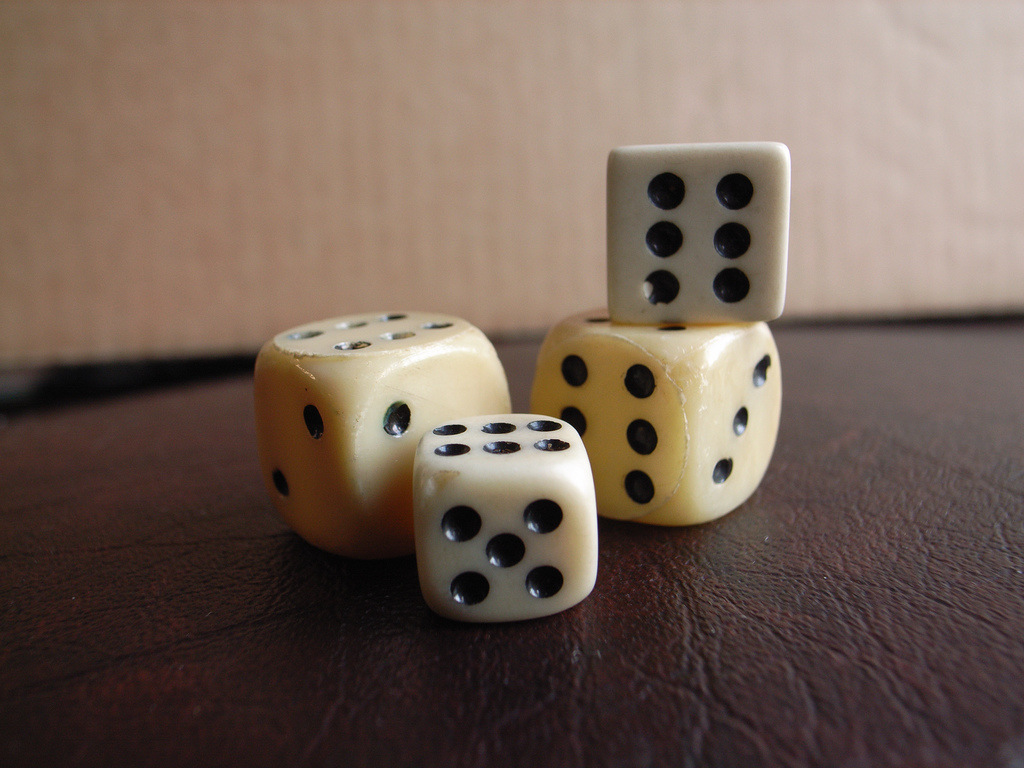
\includegraphics[width=0.95\textwidth]{/part04/dice.jpg}
 \begin{center}
 {\large ``Our life is on dice''}
 \par
 Foto di matsuyuki
 \par
 \url{http://www.flickr.com/photos/matsuyuki/201651074//}\par
 Licenza: Attribuzione 2.0 (CC BY SA 2.0)\par
 \end{center}
\clearpage
\cleardoublepage

% (c)~2014 Claudio Carboncini - claudio.carboncini@gmail.com
% (c)~2014 Dimitrios Vrettos - d.vrettos@gmail.com
\chapter{La probabilità}
\section{Gli eventi}
L'esito del lancio di una moneta o di un dado, l'esito di un'estrazione del lotto, il sesso di un nascituro, la durata di una lampadina o di un computer sono esempi di fenomeni la cui realizzazione non può essere prevista con certezza; per questo vengono detti eventi casuali o aleatori (dal latino \emph{alea} che significa ``dado''). Spesso è necessario prendere decisioni in condizioni di incertezza: in quale università proseguire gli studi, decidere se fare il vaccino contro l'influenza, scommettere sulla vincita di una squadra, sull'uscita di una sequenza di numeri al gioco del lotto, \ldots{} \`E quindi fondamentale nei confronti di un fenomeno dall'esito incerto, poter identificare quali sono gli eventi che si possono verificare ed inoltre riuscire ad esprimere il proprio grado di fiducia nel verificarsi di tali eventi.

Quali sono gli eventi possibili per un dato fenomeno aleatorio? Supponiamo di lanciare un dado e di essere interessati alla faccia che si presenta dopo aver effettuato il lancio. Il lancio del dado rappresenta l'esperimento oggetto del nostro studio, l'uscita del numero 4 o l'uscita di un numero dispari sono detti \emph{eventi aleatori} o \emph{casuali}, in quanto sappiamo che si presenterà una delle facce, ma non sappiamo quale.

\begin{definizione}
Si chiama \emph{evento} il risultato di un \emph{fenomeno aleatorio}.
\end{definizione}

Se si considera la proposizione ``Oggi farà bel tempo'' è evidente che non è chiaro cosa si intende per bel tempo (senza pioggia? senza nuvole? con il sole?) né il luogo a cui ci si riferisce. Sarebbe meglio affermare per esempio ``Stamani a Milano ci sarà il sole''. \`E necessario quindi specificare con precisione l'evento che si considera in modo da essere sicuri se l'evento si è verificato o meno.

Nel lancio di un dado sono possibili sei risultati, espressi dai numeri da 1 a 6 e solo uno di essi si realizzerà.

Chiamiamo questi sei risultati \emph{eventi elementari} e indichiamo il loro insieme con 
\[\Omega =\{1\text{, }2\text{, }3\text{, }4\text{, }5\text{, }6\}.\]

\begin{definizione}
Si chiama \emph{spazio degli eventi}, l'insieme di tutti gli esiti possibili del fenomeno considerato. Tale insieme viene indicato con $\Omega$.
\end{definizione}

L'insieme $\Omega$ non esaurisce la totalità degli eventi collegati al lancio del dado; non comprende per esempio l'evento $P=\text{numero pari}$ o l'evento $M=\text{numero minore di }3$. Tuttavia $\Omega$ permette di rappresentare qualsiasi evento come suo particolare sottoinsieme.

\begin{definizione}
Si chiama \emph{evento elementare} ogni elemento dell'insieme $\Omega$, mentre \emph{evento composto} un sottoinsieme qualsiasi di $\Omega$.
\end{definizione}

Estraiamo una carta da un mazzo di 52 carte e consideriamo i seguenti eventi: ``uscita di un asso di cuori'' e ``uscita di un re''. Qual è la differenza fra questi due eventi? Il primo dei due è un evento elementare, mentre l'altro è un evento formato da quattro eventi elementari (tutti i possibili re presenti nel mazzo) e quindi è un evento composto.

Sono esempi di eventi composti l'uscita di un numero dispari nel lancio di un dado o l'estrazione di due palline rosse da un'urna contenente 3 palline rosse e 7 nere.

Consideriamo ora due eventi che rivestono una particolare importanza: l'uscita del 7 nel lancio di un dado e l'uscita di un numero minore di 7, sempre nel lancio di un dado. È evidente che l'uscita del 7 non si verificherà mai, mentre l'uscita di un numero minore di 7 è un evento sempre verificato.

\begin{definizione}
Chiamiamo \emph{evento impossibile}, e lo indicheremo con $\emptyset$, un evento che non può verificarsi in alcun caso.
Chiamiamo \emph{evento certo} un evento che accade sicuramente e che è costituito dall'insieme di tutti gli eventi elementari di $\Omega$, cioè da tutti gli esiti possibili del fenomeno considerato.
\end{definizione}

Gli eventi elementari di un insieme $A$ e gli eventi composti che si possono ottenere con gli eventi elementari di $A$ formano lo \emph{spazio degli eventi} che viene indicato con $\wp(A)$.

Gli eventi sono gli oggetti dello studio della probabilità e in genere si indicano con le lettere maiuscole $A$, $B$, \ldots{} mentre per le operazioni e le relazioni tra eventi si usano i corrispondenti simboli che si sono utilizzati per le operazioni e le relazioni tra insiemi. Molto utile è anche la rappresentazione con i diagrammi di Venn (figura~\ref{fig:9.1}).

\begin{figure}[tp]
\begin{minipage}[t]{.45\textwidth}
\centering% (c) 2013 Claudio Carboncini - claudio.carboncini@gmail.com
\begin{tikzpicture}[x=10mm,y=10mm,font=\small]
\definecolor{circle area}{gray}{0.9}
\draw[rounded corners, fill=circle area] (0,0) rectangle (4,3) (-.2,3) node {$\Omega$} ;
\node[]  at (.5,.4) {$\bar{A}$};
\draw[fill=white](2,1.5) circle (1) (2,1.5) node {$A$};
\end{tikzpicture}

\caption{La \emph{negazione} di un evento $A$, indicata con $\bar {A}$, è l'evento che si verifica quando non si verifica $A$.}\label{fig:9.1}
\end{minipage}\hfil
\begin{minipage}[t]{.45\textwidth}
\centering% (c) 2013 Claudio Carboncini - claudio.carboncini@gmail.com
\begin{tikzpicture}[filled/.style={fill=circle area, draw=circle edge, thick},x=10mm,y=10mm,font=\small]
\def\firstcircle{(1.4,1.5) circle (1cm)}
\def\secondcircle{(2.7,1.5) circle (1cm)}

\definecolor{circle edge}{gray}{0.9}
\definecolor{circle area}{gray}{0.9}
    \begin{scope}
        \clip \firstcircle;
        \fill[filled] \secondcircle;
    \end{scope}
    \draw\firstcircle node {$A$};
    \draw \secondcircle node {$B$};
    \node[anchor=south] at (current bounding box.north) {$A \cap B$};
\draw[rounded corners] (0,0) rectangle (4,3) (-.2,3) node {$\Omega$} ;

\end{tikzpicture}

\caption{L'\emph{intersezione} tra gli eventi $A$ e $B$ indicata con $C=A\cap B$ è l'evento che si verifica quando si verificano sia $A$ che $B$.}
\end{minipage}
\vspace{5px}
\begin{minipage}[t]{.45\textwidth}
\centering% (c) 2013 Claudio Carboncini - claudio.carboncini@gmail.com
\begin{tikzpicture}[filled/.style={fill=circle area, draw=black, thin},x=10mm,y=10mm,font=\small]

\def\firstcircle{(1.4,1.5) circle (1cm)}
\def\secondcircle{(2.7,1.5) circle (1cm)}

\definecolor{circle area}{gray}{.9}

 \draw[filled] \firstcircle node {$A$}
                  \secondcircle node {$B$};
 \node[anchor=south] at (current bounding box.north) {$A \cup B$};
\draw[rounded corners] (0,0) rectangle (4,3) (-.2,3) node {$\Omega$} ;

\end{tikzpicture}

\caption{L'\emph{unione} tra gli eventi $A$ e $B$ indicata con $C=A\cup B$ è l'evento che si verifica quando si verifica almeno uno dei due eventi.}
\end{minipage}\hfil
\begin{minipage}[t]{.45\textwidth}
\centering% (c) 2013 Claudio Carboncini - claudio.carboncini@gmail.com
\begin{tikzpicture}[filled/.style={fill=circle area, draw=black, thin},x=10mm,y=10mm,font=\small]
\def\firstcircle{(2,1.5) circle (1.1cm)}
\def\secondcircle{(1.8,1.4) circle (.7cm)}

\definecolor{circle edge}{gray}{0.9}
\definecolor{circle area}{gray}{0.9}
    \begin{scope}
        \clip \firstcircle;
        \fill[filled] \secondcircle;
    \end{scope}
    \draw\firstcircle;
    \node[]  at (2.7,1.8) {$B$}; 
    \draw \secondcircle node {$A$};
    \node[anchor=south] at (current bounding box.north) {$A \to B$};
\draw[rounded corners] (0,0) rectangle (4,3) (-.2,3) node {$\Omega$} ;

\end{tikzpicture}

\caption{L'evento $A$ \emph{implica} l'evento $B$, in simboli $ A \subseteq B$, se ogni volta che si verifica $A$ si verifica anche $B$.}
\end{minipage}
\vspace{5px}
\begin{minipage}[t]{.45\textwidth}
\centering% (c) 2013 Claudio Carboncini - claudio.carboncini@gmail.com
\begin{tikzpicture}[filled/.style={fill=circle area, draw=circle edge, thick},x=10mm,y=10mm,font=\small]
\def\firstcircle{(1.1,1.5) circle (.8cm)}
\def\secondcircle{(2.9,1.5) circle (.8cm)}

\definecolor{circle edge}{gray}{0.8}
\definecolor{circle area}{gray}{0.8}
    \begin{scope}
        \clip \firstcircle;
        \fill[filled] \secondcircle;
    \end{scope}
    \draw\firstcircle node {$A$};
    \draw \secondcircle node {$B$};
    \node[anchor=south] at (current bounding box.north) {$A \cap B=\emptyset$};
\draw[rounded corners] (0,0) rectangle (4,3) (-.2,3) node {$\Omega$} ;

\end{tikzpicture}

\caption{Due eventi $A$ e $B$ si dicono \emph{incompatibili}, se il verificarsi dell'uno esclude il verificarsi dell'altro.}
\end{minipage}\hfil
\begin{minipage}[t]{.45\textwidth}
\centering% (c) 2013 Claudio Carboncini - claudio.carboncini@gmail.com
\begin{tikzpicture}[x=10mm,y=10mm,font=\small]
\draw[rounded corners] (0,0) rectangle (4,3) (-.2,3) node {$\Omega$} ;
\draw (.5, 3) .. controls(2,1) .. (1.5, 0);
\node at (.5,1.4) {$A$};
\draw (2.5, 3) .. controls(.5,1.5) .. (2.5, 0);
\node at (2.7,2.6) {$B$};
\draw (2.8,1.5) ellipse (1 and .7);
\node at (2.6,1.5) {$C$};
\draw (3.5,3) -- (2.5,0);
\node at (3.5,.5) {$D$};
\node at (1.9,.18) {$E$};
\node at (1.4,2.6) {$F$};
\end{tikzpicture}

\caption{Due o più eventi si dicono \emph{esaustivi}, se almeno uno di essi si verifica. L'unione di tali eventi coincide con l'insieme $\Omega$.}
\end{minipage}
\vspace{5px}
\begin{minipage}[t]{.90\textwidth}
\centering% (c) 2013 Claudio Carboncini - claudio.carboncini@gmail.com
\begin{tikzpicture}[x=10mm,y=10mm,font=\small]
\draw[rounded corners] (0,0) rectangle (4,3) (-.2,3) node {$\Omega$} ;
%insiemi F ed E
\draw [name path=curva1] (.5, 3) .. controls(2,1) .. (1.5, 0);
\draw [color=white, name path=curva2] (2.5, 3) .. controls(.5,1.5) .. (2.5, 0);
\coordinate [name intersections={of=curva1 and curva2, by={a,b}}];
\draw (a) -- (2.5,3);
\draw (b) -- (2.5,0);
%insiemi B ed D
\draw [name path=elipse1] (2.8,1.5) ellipse (1 and .7);
\draw [color=white, name path=linea1] (3.5,3) -- (2.5,0);
\coordinate [name intersections={of=elipse1 and linea1, by={c,d}}];
\draw (c) -- (3.5,3);
\draw (d) -- (2.5,0);

\node at (.5,1.4) {$A$};
\node at (2.7,2.6) {$B_1$};
\node at (2.6,1.5) {$C$};
\node at (3.5,.5) {$D_1$};
\node at (1.9,.18) {$E$};
\node at (1.4,2.6) {$F$};
\end{tikzpicture}

\caption{Un insieme di eventi formato da eventi tra loro incompatibili ed esaustivi, genera una partizione nello spazio degli eventi.}
\end{minipage}\hfil
\end{figure}

\begin{definizione}
Se $n$ eventi $E_1$, $E_2$, \ldots, $E_n$ sono esaustivi cioè $E_1 \cup E_2 \cup \dots{} \cup E_n=\Omega$ e a due a due tra loro incompatibili $E_1\cap E_2 = E_1 \cap E_3 = \ldots = E_1 \cap E_n = E_2 \cap E_3 = \ldots = E_2 \cap E_4 = \ldots = E_2 \cap E_n = \ldots = E_{n-1}\cap E_n=\emptyset$) diremo che essi formano una \emph{partizione dello spazio degli eventi}. Gli eventi, identificabili da tutti i possibili sottoinsiemi di $\Omega$, sono dati dall'\emph{insieme delle parti} di $\Omega$ indicato con $\wp (\Omega).$
\end{definizione}

Ricordiamo che la cardinalità dell'insieme delle parti cioè il numero degli eventi che si possono formare con gli elementi di $\Omega$ è dato da $\card(\wp(\Omega ))=2^n$, dove $n$ rappresenta il numero degli eventi elementari. Così nel lancio del dado abbiamo $2^6=64$ possibili eventi, considerando anche l'insieme vuoto $\emptyset$ che rappresenta l'evento impossibile e l'insieme $\Omega =\{1$, 2, 3, 4, 5, $6\}$ che rappresenta l'evento certo.

\vspazio\ovalbox{\risolvii \ref{ese:9.1}, \ref{ese:9.2}, \ref{ese:9.3}, \ref{ese:9.4}, \ref{ese:9.5}}

\section{Definizioni di probabilità}

Nel linguaggio comune l'uso del termine probabilità è abbastanza chiaro e uniforme. Si dice che un certo fatto o evento è più o meno probabile a seconda che ci si aspetti che si verifichi più o meno facilmente.

La probabilità è dunque una misura del grado di fiducia associato al verificarsi di un evento e dipende dalle informazioni che si hanno a disposizione al momento di effettuare la valutazione.

Se diciamo che oggi pioverà con probabilità $\np{0,20}=\frac{20}{100}=\frac 1 5$ intendiamo che siamo disposti a scommettere 20 centesimi per avere 1 euro nel caso che piova e perdere i 20 centesimi della posta nel caso che non piova.

\begin{definizione}
La valutazione della probabilità dell'evento $E$ è quel valore $P(E)$ che si ottiene dalla quota $q$ che l'individuo che procede alla valutazione è disposto a pagare per ricevere una vincita $S$ nel caso si verifichi l'evento. Quindi $P(E)=\dfrac q S$.
\end{definizione}

Per ottenere una valutazione coerente, per valutare quanto siamo disposti a perdere/{}vincere nella scommessa, dobbiamo immedesimarci nei due ruoli, quello dello scommettitore e quello del banco. Inoltre le somme che scommettiamo devono essere significative per chi procede alla valutazione.
Nessun individuo coerente scommetterebbe su un evento impossibile una quota maggiore di 0 qualunque sia la vincita e nessun individuo pagherebbe una vincita per il verificarsi di un evento certo.
Da queste considerazioni deduciamo che la misura della probabilità appartiene all'intervallo $[0$, $1]$, essendo $0$ il valore che corrisponde all'evento impossibile e $1$ quello che corrisponde all'evento certo.

\begin{postulato}[sulla probabilità]\label{post:probabilita}
La probabilità di un evento $E$ è un numero reale compreso tra $0$ e $1$: $0\le P(E)\le 1$;

La probabilità dell'evento impossibile è $0$: $P(\emptyset)=0$;

La probabilità dell'evento certo è uguale a $1$: $P(\Omega)=1$.
\end{postulato}

\subsection{La valutazione classica}

La valutazione della probabilità a volte si riconduce a semplici giudizi di equiprobabilità: cioè ogni evento elementare dello spazio degli eventi ha la stessa probabilità. Così nel lancio di un dado, nel gioco della tombola, nel gioco delle carte tutti gli eventi elementari hanno la stessa probabilità. Quindi se $n$ sono gli eventi elementari la probabilità di ciascuno di essi è $\frac 1 n$.

La probabilità di un evento $E$ è data dal rapporto tra il numero $f$ dei casi favorevoli al verificarsi di $E$ e il numero $n$ di tutti i casi possibili, purché ugualmente possibili. In simboli: \[P(E)=\dfrac f n.\]

Mentre nei giochi di sorte si realizzano le condizioni per calcolare tale probabilità (conoscenza a priori dei casi possibili, di quelli favorevoli e condizione di equiprobabilità) esistono altri eventi casuali per i quali è difficile o impossibile calcolare tale probabilità.

\begin{exrig}
\begin{esempio}
Se in un sacchetto ho 3 palline rosse e 2 palline gialle qual è la probabilità che estraendo a caso una pallina questa sia rossa?

La probabilità che si estragga una pallina rossa è $p=\frac 3 5=\np{0,6}=60\text{\%}$, infatti i casi favorevoli al verificarsi dell'evento ``estrarre una pallina rossa'' sono 3, tante quante sono le palline rosse, i casi possibili, tutti ugualmente possibili, sono 5, tante quante palline ci sono nel sacchetto.
\end{esempio}

\begin{esempio}
Da un mazzo di 40 carte napoletane estraiamo una carta. Calcoliamo la probabilità degli eventi:
\begin{itemize*}
\item $A=$ esce una carta di spade;
\item $B=$ esce una carta con il numero 12;
\item $C=$ esce una carta con un numero o una figura;
\item $D=$ esce il sette di denari;
\item $E=$ esce un asso.
\end{itemize*}
I casi possibili sono 40, dato che il mazzo è formato da 40 carte. Anche qui siamo in presenza di eventi elementari equiprobabili, applichiamo ancora lo schema di valutazione classico
\begin{itemize*}
\item L'evento $A$ è casuale, infatti i casi favorevoli sono 10, dato che il mazzo ha 10 carte di spade: $P(A)=\frac{10}{40}=\frac 1 4$;
\item l'evento $B$ è impossibile dato che non esiste una carta col numero 12: $P(B)=0$;
\item l'evento $C$ è certo, infatti i casi favorevoli sono 40, dato che il mazzo ha 12 figure e 28 carte con un numero: $P(C)=1$;
\item c'è un solo sette di denari su 40 carte: $P(D)=\frac 1{40}$;
\item nel mazzo di 40 carte ci sono 4 assi: $P(E)=\frac 4{40}=\frac 1{10}=\np{0,1}=10\%$;
\end{itemize*}
\end{esempio}

\begin{esempio}
Lanciando in aria 3 monete, quale dei seguenti eventi è più probabile?
\begin{itemize*}
\item Ottenere su 3 monete testa;
\item ottenere su 1 moneta testa e su 2 monete croce.
\end{itemize*}
Per rispondere alla domanda occorre calcolare le probabilità dei due eventi. Applichiamo la definizione classica. Dobbiamo calcolare tutti gli eventi possibili e tutti gli eventi favorevoli.
Aiutiamoci con una tabella per elencare tutti i casi.

\begin{center}
\begin{tabular}{ccc}
prima moneta & seconda moneta & terza moneta\\
\boxT & \boxT & \boxT\\
\boxT & \boxT & \boxC\\
\boxT & \boxC & \boxT\\
\boxT & \boxC & \boxC\\
\boxC & \boxT & \boxT\\
\boxC & \boxT & \boxC\\
\boxC & \boxC & \boxT\\
\boxC & \boxC & \boxC\\
\end{tabular}
\end{center}
I casi possibili sono 8. C'è un solo caso favorevole all'evento ``3 volte testa''. La probabilità di questo evento è quindi $p=\frac 1 8=\np{0,125}=\np{12,5}\%$.

I casi favorevoli all'evento ``1 moneta testa e 2 monete croce'' sono CCT, CTC, TCC, quindi 3, allora $p=\frac 3 8=\np{0,375}=\np{37,5}\%$. Possiamo concludere che l'evento più probabile è ottenere 1 testa e 2 croci.
\end{esempio}
\end{exrig}

\subsection{La valutazione sperimentale}

Se si considera una successione di eventi dello stesso tipo e che avvengono in condizioni simili come l'uscita di una determinata faccia in un dado truccato, si indica come frequenza relativa $F(E)$ il rapporto tra il numero $v$ dei casi in cui si è verificato l'evento e il numero totale delle prove $n$, cioè $F(E)=\dfrac v n$.

In una serie di prove ripetute nelle stesse condizioni, la frequenza relativa di un evento tende a stabilizzarsi intorno a un valore ben preciso al crescere del numero delle prove effettuate.
Si assume come valutazione della probabilità dell'evento $E$ il valore intorno al quale tende a stabilizzarsi la frequenza relativa dello stesso evento, all'aumentare del numero delle prove ripetute alle stesse condizioni: $P(E)\approx F(E)=\dfrac v n$.
L'errore che si commette diventa sempre più piccolo al crescere di $n$. La valutazione della probabilità così definita si chiama \emph{valutazione sperimentale}, \emph{statistica}, \emph{a posteriori} o \emph{frequentista}.

Anche l'ambito di applicazione di tale valutazione è limitato in quanto l'ipotesi che sta alla base della definizione è che l'evento a cui si vuole assegnare la probabilità sia pensabile come uno dei possibili risultati di una determinata prova e che tale prova sia ripetibile infinite volte nelle stesse identiche condizioni.
Si fa molto uso di questo schema di valutazione per stime della probabilità in campo economico e sanitario.

\begin{exrig}
\begin{esempio}
In un'azienda alimentare si producono vasetti di marmellata. In uno studio di controllo effettuato su \np{2500} vasetti ne sono stati evidenziati 13 con imperfezioni e non idonei al commercio. Si valuti la probabilità dell'evento $E=$``confezioni non idonee al commercio''.

Se si considera il campione dei vasetti analizzati significativo rispetto alla produzione complessiva delle confezioni prodotte, possiamo considerare la frequenza relativa dell'evento $E$ come misura della probabilità. Quindi $P(E)=F(E)=\frac{13}{\np{2500}}=\np{0,0052}=\np{0,52}\%$.
\end{esempio}

\begin{esempio}
Qual è la probabilità che un certo guidatore faccia un incidente con la macchina? Quanto deve pagare, come premio a una compagnia di assicurazioni, in modo che, se fa un incidente, la compagnia paghi per intero il danno?

Per rispondere a queste domande le compagnie di assicurazioni sono in grado di stimare, sulla base dei numerosissimi incidenti stradali che si verificano ogni anno, qual è la probabilità che un guidatore provochi un incidente d'auto.
\end{esempio}

\begin{esempio}
Un sacchetto contiene 10 palline, alcune bianche, altre nere. Si estrae a caso, senza guardare nel sacchetto un pallina, si guarda il colore e si rimette il sacchetto nella pallina.

Dopo 100 estrazioni abbiamo contato 78 volte la pallina bianca e 22 la pallina nera. Possiamo allora ipotizzare che nel sacchetto ci siano 8 palline bianche e 2 palline nere.
\end{esempio}
\end{exrig}

\subsection{La valutazione soggettiva}

La valutazione soggettiva della probabilità è la definizione che abbiamo dato all'inizio del capitolo: la probabilità dell'evento $A$ è quel valore $p$ che l'individuo che procede alla valutazione è disposto a pagare per ricevere una vincita unitaria. Se un individuo valuta pari $\frac 1 4=25\%$ la probabilità di un certo evento $E$ vuol dire che è disposto a pagare $25$ euro a un ipotetico banco per riceverne $100$ nel caso che $E$ si verifichi. Naturalmente la scommessa va accettata anche come banco che deve essere disposto a scommettere il $75\%=1-p$ sul fatto che $E$ non si verifichi: $P(E)=\frac q S$ con $ q=25 $ e $S=100$.

\subsubsection*{Le scommesse}

La definizione soggettiva si applica anche alle scommesse. Supponiamo di scommettere sul verificarsi di un evento $E$ a cui attribuiamo probabilità $p$. Stabiliamo inoltre di giocare e quindi perdere $q$ euro nel caso l'evento non si verifichi e di guadagnare $g$ euro nel caso l'evento si verifichi. In genere le scommesse si indicano in questo modo: si mette in rapporto il guadagno con la perdita $\frac g q$ o anche $g:q$ che si legge $g$ a $q$. In questo caso $q$ e $g$ si chiamano le \emph{poste} o le \emph{messe} del gioco.

%si mette in rapporto la perdita con il guadagno $\frac q g$ o anche $q:g$ che si legge $q$ a $g$. In questo caso $q$ e $g$ si chiamano le \emph{poste} o le \emph{messe} del gioco.

Che relazione c'è tra questo rapporto e la probabilità?

Se in un grande numero $n$ di scommesse così congegnate vincessimo la somma $g$ per $np$ di volte e perdessimo la somma $q$ per $n(1-p)$ volte, affinché il gioco risulti \emph{equo} dovremmo avere $np\cdot g-nq\cdot (1-p)=0 \:\Rightarrow\: n(p\cdot g-q\cdot (1-p))=0$ e visto che $n\neq 0$ si può dividere per $n$ ottenendo $p\cdot g-q\cdot (1-p)=0$. Isoliamo $p$ nell'uguaglianza:
\begin{equation*}
p\cdot g-q\cdot (1-p)=0 \:\Rightarrow\: p\cdot g-q+q\cdot p=0\:\Rightarrow\: p\cdot (g+q)=q \:\Rightarrow\: p=\frac q{g+q}.
\end{equation*}
La relazione è dunque questa: la probabilità di una scommessa $g:q$ è data dalla perdita $q$ al numeratore e al denominatore la somma complessiva che si incassa data dal guadagno più quello che si è scommesso.

\begin{exrig}
\begin{esempio}
Supponiamo che la vincita ai mondiali di calcio dell'Italia sia data $12:5$, cioè 12 a 5, dai bookmaker inglesi. Quale probabilità assegnano gli allibratori alla vincita dell'Italia?

Significa che scommettendo 5 euro sulla vincita dell'Italia ne possiamo vincere 12 nel caso che l'evento si verifichi.

Quindi la probabilità della vincita dell'Italia sarà:
$P(E)=\frac 5{5+12}=\frac 5{17}=\np{0,294}=\np{29,4}\%$
\end{esempio}

\begin{esempio}
Leggo sul sito del Corriere della Sera, che per la partita Real Madrid-Barcellona, che si giocherà questa sera, la vittoria del Real Madrid viene data \np{2,60} a 1.

Significa che scommettendo 1 euro possiamo vincerne \np{2,60}: la vittoria del Real Madrid è stata quindi stimata dal giornale $p=\frac 1{\np{2,60}}=\frac{100}{260}=\np{0,38}\ldots$ circa 38\%.
\end{esempio}
\end{exrig}
\ovalbox{\risolvii \ref{ese:9.6}, \ref{ese:9.7}, \ref{ese:9.8}, \ref{ese:9.9}, \ref{ese:9.10}, \ref{ese:9.11}, \ref{ese:9.12}, \ref{ese:9.13}, \ref{ese:9.14}, \ref{ese:9.15}, \ref{ese:9.16},}

\vspazio\ovalbox{\ref{ese:9.17}, \ref{ese:9.18}, \ref{ese:9.19}, \ref{ese:9.20}, \ref{ese:9.21}, \ref{ese:9.22}, \ref{ese:9.23}, \ref{ese:9.24}, \ref{ese:9.25}, \ref{ese:9.26}, \ref{ese:9.27}}

\section{Probabilità dell'unione di due eventi}

La misura della probabilità si può applicare a tutti gli eventi individuati dall'insieme delle parti degli eventi elementari $\wp(\Omega)$. Qualsiasi evento si può definire come sottoinsieme dell'insieme elementare (elencando gli eventi elementari che ne fanno parte) oppure enunciando una proposizione vera nel caso in cui l'evento si verifichi. Possiamo quindi poter esprimere la probabilità su eventi composti da due o più eventi di $\wp(\Omega)$ attraverso le operazioni di unione e intersezione tra insiemi che corrispondono alle operazioni di disgiunzione inclusiva e di congiunzione nelle proposizioni.

Per la probabilità dell'evento unione di due eventi occorre distinguere tra eventi tra loro \emph{incompatibili} ed eventi tra loro \emph{compatibili}.

\subsection[Unione di due eventi tra loro incompatibili]{Unione di due eventi tra loro incompatibili}

\begin{definizione}
Due eventi $A$ e $B$ si dicono \emph{incompatibili} quando non si possono verificare contemporaneamente, cioè quando $A\cap B=\emptyset$.
\end{definizione}

\begin{definizione}
Due eventi $A$ e $B$ si dicono \emph{compatibili} quando si possono verificare contemporaneamente, cioè quando $A\cap B\neq \emptyset$.
\end{definizione}
\pagebreak
\begin{exrig}
\begin{esempio}
Nel lancio di un dado regolare calcolare la probabilità dell'uscita del numero 3 o di un numero pari.

I due eventi $A=$``uscita del numero 3'' e $B=$``uscita di un numero pari'' sono eventi incompatibili.

Ci sono due modi per calcolare la probabilità dell'evento unione.
\paragraph{Modo I}: Secondo la valutazione classica la probabilità che esca il $3$ o un numero pari è uguale a $\frac 4 6$: infatti i casi favorevoli sono 4 (le facce 3, 2, 4 e 6) su un totale di $6$ casi possibili.
\paragraph{Modo II}: Calcoliamo la probabilità dell'unione dei due eventi considerando le proprietà dei singoli eventi. Dato che i due eventi sono incompatibili, cioè: $A\cap B=\emptyset $: abbiamo $P(A\cup B)=\frac 1 6+\frac 3 6=\frac 4 6$.
\begin{center}
 % (c) 2013 Claudio Carboncini - claudio.carboncini@gmail.com
\begin{tikzpicture}[x=10mm,y=10mm,font=\small]
\def\insieme_unione{(1.9,1.6) ellipse (1.7 and 1.3)}
\def\insiemeB{(1.5,2) ellipse (.9 and .7)}
\def\insiemeA{(2.3,.9) ellipse (.7 and .4)}
\draw[rounded corners] (0,0) rectangle (4,3) (-.2,3) node {$\Omega$} ;
\draw\insieme_unione;
\draw\insiemeB node {$B$};
\draw\insiemeA node {$A$};
\draw[fill=blue] (.9,2.3)circle (1.5pt) node[right]{$2$};
\draw[fill=blue] (.9,1.8)circle (1.5pt) node[right]{$6$};
\draw[fill=blue] (2,2)circle (1.5pt) node[right]{$4$};
\draw[fill=blue] (1.8,.8)circle (1.5pt) node[right]{$3$};
\draw[fill=blue] (.3,.3)circle (1.5pt) node[right]{$1$};
\draw[fill=blue] (3.6,2.7)circle (1.5pt) node[right]{$5$};
\node at (3,1.6) {$A \cup B$};
\end{tikzpicture}

\end{center}
\end{esempio}
\end{exrig}

Possiamo quindi affermare che dati due eventi incompatibili cioè tali che $A\cap B=\emptyset$ la probabilità dell'evento unione è dato dalla uguaglianza: $P(A\cup B)=P(A)+P(B)$.

Può essere utile per avere un'idea intuitiva di questa uguaglianza pensare alla probabilità come una massa unitaria distribuita sugli eventi. Se voglio la probabilità di $A\cup B$, considero la massa presente su $A$ che addiziono a quella presente su $B$ (in analogia al caso dell'unione di insiemi disgiunti).

\subsection{Unione di due eventi tra loro compatibili}

\begin{exrig}
\begin{esempio}
Consideriamo il lancio di un dado regolare, vogliamo trovare la probabilità dell'uscita di un numero maggiore di 2 o di un numero dispari.

Gli eventi $A=$``uscita di un numero maggiore di 2'' e $B=$``uscita di un numero dispari'' sono compatibili in quanto le facce 5 e 3 appartengono sia all'evento $A$ che all'evento $B$.
\begin{center}
 % (c) 2013 Claudio Carboncini - claudio.carboncini@gmail.com
\begin{tikzpicture}[x=10mm,y=10mm,font=\small]

\def\insiemeA{(1.5,1.9) ellipse (1.2 and .8)}
\def\insiemeB{(2.3,1) ellipse (1.1 and .9)}
    \begin{scope}
        \clip \insiemeA;
        \fill[color=gray!20!] \insiemeB;
    \end{scope}
\draw[rounded corners] (0,0) rectangle (4,3) (-.2,3) node {$\Omega$} ;
\draw\insiemeB node {$B$};
\draw\insiemeA node {$A$};
\draw[fill=blue] (.9,2.2)circle (1.5pt) node[right]{$6$};
\draw[fill=blue] (3.4,2.3)circle (1.5pt) node[right]{$2$};
\draw[fill=blue] (1.9,2.3)circle (1.5pt) node[right]{$4$};
\draw[fill=blue] (2.7,.7)circle (1.5pt) node[right]{$1$};
\draw[fill=blue] (2,1.6)circle (1.5pt) node[right]{$3$};
\draw[fill=blue] (1.5,1.4)circle (1.5pt) node[right]{$5$};

\end{tikzpicture}

\end{center}
\paragraph{Modo I}: La probabilità che esca un numero maggiore di $2$ o un numero dispari è uguale a $\frac 5 6$: infatti i casi favorevoli sono 5 (le facce 1, 3, 4, 5 e 6) su un totale di $6$ casi possibili.
\paragraph{Modo II}: Calcoliamo la probabilità dell'unione dei due eventi considerando le proprietà dei singoli eventi. In questo caso non possiamo sommare come nei casi precedenti le probabilità dei singoli eventi. Infatti $P(A)+P(B)=\frac 4 6+\frac 3 6=\frac 7 6$ che contraddice l'assioma della probabilità. Occorre togliere la probabilità dell'intersezione tra $A$ e $B$ contata due volte, una volta per $A$ e una per $B$, che è uguale a $\frac 2 6$: due casi favorevoli (le facce 3 e 5) su sei casi possibili: \[P(A\cup B)=P(A)+P(B)-P(A\cap B)=\frac 4 6+\frac 3 6-\frac 2 6=\frac 5 6.\]
\end{esempio}

\begin{esempio}
Calcolare la probabilità che estraendo a caso un numero della tombola esso contenga la cifra 5 oppure sia multiplo di 5.

La prima domanda da farsi è se i due eventi sono compatibili o incompatibili. Poiché esistono numeri della tombola che contengono la cifra 5 e che sono anche multipli di 5 (per esempio 15, 50, \ldots) i due eventi sono compatibili. Di conseguenza bisogna applicare la regola $P(A\cup B)=P(A)+P(B)-P(A\cap B)$.
\begin{itemize*}
\item $A=$``estrarre un numero che contiene la cifra 5''. Questi numeri sono: 5, 15, 25, 35, 45, 50, 51, 52, \ldots, 59, 65, 75, 85, in tutto 18 ne segue che: $p(A)=\frac{18}{90}$;
\item $B=$``estrarre un numero multiplo di 5''. I multipli di 5 sono 5, 10, 15, 20, \ldots{} due per ogni decina, quindi 18 in tutto, ne segue che: $p(B)=\frac{18}{90}$;
\item $A\cap B=$``estrarre un cifra che contiene 5 ed è multiplo di 5''. Questi numeri sono 5, 15, 25, 35, 45, 50, 55, 65, 75, 85 in tutto sono 10 quindi: $p(A\cap B)=\frac{10}{90}$.
\end{itemize*}
Applichiamo la regola della probabilità utilizzata nel modo II del precedente esempio quindi:

$A\cup B=$``estrarre un numero che contenga la cifra 5 oppure sia multiplo di 5''. \[P(A\cup B)=P(A)+P(B)-P(A\cap B)=\frac{18}{90}+\frac{18}{90}-\frac{10}{90}=\frac{26}{90}\simeq \np{0,29}= 29\%. \]
\end{esempio}
\end{exrig}

Dagli esempi svolti possiamo enunciare il seguente teorema:

\begin{teorema}[delle probabilità totali]
Dati due eventi $A$ e $B$, entrambi appartenenti allo stesso spazio degli eventi, la probabilità dell'unione degli eventi è uguale alla somma delle probabilità dei singoli eventi meno la probabilità della loro intersezione.
In simboli: \[P(A\cup B)=P(A)+P(B)-P(A\cap B).\]
\end{teorema}

Se pensiamo alla probabilità come una massa unitaria distribuita sugli eventi, per calcolare la probabilità di $A\cup B$, considero la massa presente su $A$ che addiziono a quella presente su $B$ a cui devo togliere la massa presente su $A\cap B$ che è stata contata due volte.

\osservazione Il teorema delle proprietà totali vale anche nel caso degli eventi incompatibili in quanto in questo caso la probabilità dell'intersezione dei due eventi $P(A\cap B)=\emptyset$ e l'uguaglianza diventa $P(A\cup B)=P(A)+P(B)$.

\vspazio\ovalbox{\risolvii \ref{ese:9.6}, \ref{ese:9.7}, \ref{ese:9.28}, \ref{ese:9.29}, \ref{ese:9.30}, \ref{ese:9.31}, \ref{ese:9.32}, \ref{ese:9.33}, \ref{ese:9.34}, \ref{ese:9.35}, \ref{ese:9.36},}

\ovalbox{\ref{ese:9.37} \ref{ese:9.38}}

\section{Probabilità dell'evento complementare }

\begin{definizione}
Dato un evento $A$, si definisce \emph{evento complementare} di $A$, indicato con $\overline A$, l'evento che si verifica quando non si verifica $A$.
\end{definizione}

\begin{teorema}[dell'evento complementare]
Dato un evento $E$, la probabilità dell'evento complementare $\overline E$ è data da $1$ meno la probabilità dell'evento $E$. In simboli: \[ P(\overline E)=1-P(E). \]
\end{teorema}
\begin{proof} Per il postulato~\ref{post:probabilita} introdotto a pagina~\pageref{post:probabilita}: \[ P(\overline E\cup E)=P(\Omega)=1; \]
per il teorema delle probabilità totali essendo i due eventi incompatibili: \[ P(\overline E\cup E)=P(\overline E)+P(E); \]
e per la proprietà transitiva dell'uguaglianza: \[ P(\overline E)+P(E)=1 \quad\Rightarrow\quad P(\overline E)=1-P(E). \]
\end{proof}

Se pensiamo all'analogia della una massa unitaria distribuita sugli eventi, la probabilità dell'evento $\overline E$ sarà data dalla massa unitaria meno la probabilità di $E$.

\begin{exrig}
\begin{esempio}
Nel lancio di due dadi regolari determina la probabilità che la somma delle facce non sia uguale a 5.

Consideriamo la probabilità che in un lancio di due dadi si abbia un punteggio uguale a 5. I casi possibili sono 36 (ogni faccia del primo dado si può associare con ognuna delle 6 facce del secondo dado), mentre i casi favorevoli all'evento sono 4, precisamente $(1$, $4)$, $(4$, $1)$, $(2$, $3)$ e $(3$, $2)$. Quindi $P(E)=\frac 4{36}=\frac 1 9$.

Per conoscere la probabilità dell'evento complementare cioè la probabilità che la somma delle due facce del dado non sia uguale a 5, risulterebbe piuttosto laborioso trovare tutti i casi in cui la somma delle due facce sia uguale a 2, 3, 4, 6, 7, 8, 9, 10, 11 e 12, si può invece applicare la regola $P(\overline E)=1-P(E)$ cioè nel nostro caso $P(\overline E)=1-P(E)=1-\frac 1 9=\frac 8 9$.
\end{esempio}
\end{exrig}

\osservazione L'uguaglianza sulla probabilità dell'evento complementare può risultare molto utile per risolvere alcuni problemi. A volte è più facile, o indispensabile, calcolare la probabilità dell'evento complementare che calcolare direttamente la probabilità dell'evento.

\vspazio\ovalbox{\risolvii \ref{ese:9.39}, \ref{ese:9.40}, \ref{ese:9.41}, \ref{ese:9.42}, \ref{ese:9.43}, \ref{ese:9.44}, \ref{ese:9.45}, \ref{ese:9.46}}

\section{La probabilità dell'evento intersezione di due eventi}

Dati due eventi $A$, $B\in \wp(\Omega)$ ci proponiamo di calcolare la probabilità dell'evento intersezione cioè $P(A\cap B)$ partendo dalla probabilità degli eventi componenti $P(A)$ e $P(B)$. Si tratta quindi di stimare con quale probabilità i due eventi avvengono congiuntamente. Occorre innanzitutto verificare che i due eventi non siano incompatibili in quanto in questo caso l'evento intersezione è impossibile.

Per la probabilità dell'intersezione di due eventi occorre distinguere tra eventi tra loro \emph{indipendenti} e eventi tra loro \emph{dipendenti}.

\subsection{Intersezione di due eventi tra loro indipendenti}

\begin{definizione}
Due eventi $A$ e $B$ si dicono \emph{indipendenti} se il verificarsi di $A$ non cambia la probabilità del verificarsi di $B$, si dicono invece \emph{dipendenti} se il verificarsi di $A$ cambia la probabilità di $B$ rispetto a quella valutata per $B$ prima del verificarsi di $A$.
\end{definizione}

%\newpage

\begin{exrig}
\begin{esempio}
Determinare la probabilità che lanciando una moneta e un dado regolari esca testa e un numero maggiore di 4.
\begin{itemize}
\item $A=$``uscita di Testa nel lancio di una moneta'' $\Rightarrow\: P(A)=\frac 1 2$;
\item $B=$``uscita di un numero maggiore di 4 nel lancio di un dado'' $\Rightarrow\: P(B)=\frac 2 6$;
\item $(A\cap B)$=``uscita di testa e di un numero maggiore di 4 nel lancio di una moneta e di un dado''.
\end{itemize}
Vediamo come determinare $P(A\cap B)$.
I due eventi $A$ e $B$ non si influenzano in quanto l'uscita di testa non modifica la probabilità dell'uscita di 4 nel lancio del dado.

Notiamo subito una situazione diversa rispetto a quella precedente dell'unione di due eventi. Nel caso precedente, lo spazio degli eventi era lo stesso per l'evento $A$, per l'evento $B$ e per l'evento unione $(A\cup B)$.
Ora invece per l'evento $A$ l'insieme degli eventi elementari è $\Omega_1=\{T$, $C\}$, per l'evento $B$ invece, l'insieme degli eventi elementari è $\Omega_2=\{1$, 2, 3, 4, 5, $6\}$. L'evento $(A\cap B)$ ha il seguente insieme degli eventi elementari: \[\Omega=\{(T;1)\text{, }(T;2)\text{, }(T;3)\text{, }(T;4)\text{, }(T;5)\text{, }(T;6)\text{, }(C;1)\text{, }(C;2)\text{, }(C;3)\text{, }(C;4)\text{, }(C;5)\text{, }(C;6)\}. \]

Lo spazio degli eventi elementari dell'intersezione è dato dal prodotto cartesiano dello spazio elementare di $A$ moltiplicato per quello di $B$. Si può calcolare la probabilità in due modi:
\paragraph{Modo I}: Si indicano i casi favorevoli e i casi possibili rispetto all'evento intersezione: i casi favorevoli all'evento sono due: $(A\cap B)=\{(T;5)\text{, }(T;6)\}$, i casi possibili sono dodici: \[\Omega=\{(T;1)\text{, }(T;2)\text{, }(T;3)\text{, }(T;4)\text{, }(T;5)\text{, }(T;6)\text{, }(C;1)\text{, }(C;2)\text{, }(C;3)\text{, }(C;4)\text{, }(C;5)\text{, }(C;6)\} \] la probabilità dell'evento intersezione è: $P(A\cap B)=\frac 2{12}=\frac 1 6$.

\begin{center}
 % (c) 2013 Claudio Carboncini - claudio.carboncini@gmail.com
\begin{tikzpicture}[x=10mm,y=10mm,font=\small]

\def\rettangolo{-- ++(3,0) -- ++(0,2) -- ++(-3,0) -- cycle}
\def\insieme_int{-- ++(4,0) -- ++(0,3) -- ++(-4,0) -- cycle}
 %insieme1
\fill[rounded corners, color=gray!20!] (0,.5) -- (0,2) -- (3,2) -- (3,1.5) -- cycle;
\draw[rounded corners] (0,0) \rettangolo;
\node at (1.5,2.2) {$P(A)=1/2$};
\draw (0,.5) -- (3,1.5);
\draw[fill=blue] (.7,1.5) circle (1.5pt) node[right] {$T$};
\draw[fill=blue] (2.3,.5) circle (1.5pt) node[right] {$C$};
%insieme 2
\fill[rounded corners, color=gray!20!] (4.5,0) -- (6.5,0) -- (6.5,1) -- (4.5,1) -- cycle;
\draw[rounded corners] (3.5,0) \rettangolo;
\draw (3.5,1) -- (6.5,1);
\foreach \x in {4.5,5.5}{
\draw (\x,0)--(\x,2);
\draw (\x,0)--(\x,2);}
\foreach \x in {3.8,4.8,5.8}
   \foreach \y in {0.5,1.5}
   { \draw[fill=blue] (\x,\y) circle (1.5pt);}
\draw node[right] at (3.8,1.5) {$2$};
\draw node[right] at (4.8,1.5) {$4$};
\draw node[right] at (5.8,1.5) {$1$};

\draw node[right] at (3.8,0.5) {$3$};
\draw node[right] at (4.8,0.5) {$6$};
\draw node[right] at (5.8,0.5) {$5$};
\node at (5,2.2) {$P(B)=2/6$};
\node at (3.25,1) {$\times$};
%insieme risultato
\fill[color=gray!20!] (8,.5) -- (8,1.5) -- (9,1.5) -- (9,.5) -- cycle;
\fill[color=gray!20!] (9,1.5) -- (9,2.5) -- (10,2.5) -- (10,1.5) -- cycle;
\draw[rounded corners] (7,-.5) \insieme_int;
\node at (9,2.7) {$P(A \cap B )=2/12$};
\node at (6.75,1) {$=$};
\foreach \x in {8,9,10}{
\draw (\x,-.5)--(\x,2.5);
\draw (\x,-.5)--(\x,2.5);
\draw (\x,-.5)--(\x,2.5);}
\foreach \y in {.5,1.5}{
\draw (7,\y)--(11,\y);
\draw (7,\y)--(11,\y);}

\foreach \x in {7.5,8.5,9.5,10.5}
   \foreach \y in {0.2,1.2,2.2}
   { \draw[fill=blue] (\x,\y) circle (1.5pt);}
\draw node[below] at (7.5,0.2) {$(T,1)$};
\draw node[below] at (8.5,0.2) {$(C,1)$};
\draw node[below] at (9.5,0.2) {$(C,2)$};
\draw node[below] at (10.5,0.2) {$(C,6)$};

\draw node[below] at (7.5,1.2) {$(T,2)$};
\draw node[below] at (8.5,1.2) {$(T,5)$};
\draw node[below] at (9.5,1.2) {$(C,3)$};
\draw node[below] at (10.5,1.2) {$(C,4)$};

\draw node[below] at (7.5,2.2) {$(T,3)$};
\draw node[below] at (8.5,2.2) {$(T,4)$};
\draw node[below] at (9.5,2.2) {$(T,6)$};
\draw node[below] at (10.5,2.2) {$(C,5)$};

\end{tikzpicture}

\end{center}

\paragraph{Modo II}: Dato che i due eventi non si influenzano, supponiamo di procedere con due scelte successive: prima il lancio della moneta con probabilità pari a $\frac 1 2$ e poi il lancio del dado con probabilità pari a $\frac 2 6$. Se si verifica il primo evento la probabilità si riduce da 1 a $\frac 1 2$ a cui devo applicare la probabilità che si verifichi il secondo evento pari a $\frac 2 6$, moltiplicando le probabilità dei singoli eventi.
\begin{itemize*}
\item $A=$``uscita di Testa nel lancio di una moneta'' $\Rightarrow\: P(A)=\frac 1 2$;
\item $B=$``uscita di un numero maggiore di 4 nel lancio di un dado'' $\Rightarrow\: P(B)=\frac 2 6$;
\item $(A\cap B)$=``uscita di testa e di un numero maggiore di 4 nel lancio di una moneta e di un dado'' $\Rightarrow\: P(A\cap B)=P(A)\cdot P(B)=\frac 1 2\cdot \frac 2 6=\frac 2{12}$.
\end{itemize*}
\end{esempio}
\end{exrig}

Generalizziamo: dati due eventi aleatori $A$ e $B$ tra loro indipendenti la probabilità dell'evento intersezione tra $A$ e $B$ è data dalla probabilità di $A$ moltiplicata per la probabilità di $B$: \[P(A\cap B)=P(A)\cdot P(B).\]\label{reg:probabilita_intersezione_eventi_indipendenti}

\subsubsection*{Diagrammi ad albero}

Una rappresentazione grafica che può risultare utile nello studio della probabilità dell'evento intersezione detto anche studio delle \emph{probabilità composte} è il diagramma ad albero. Le linee dell'albero si dicono \emph{rami}, mentre i punti da cui partono e arrivano i rami si dicono \emph{nodi}, il nodo iniziale si chiama \emph{radice}.

La costruzione di un diagramma ad albero nel caso delle probabilità composte consente di eseguire un'analisi completa di tutti i possibili esiti di una prova. Ogni percorso dell'albero che va dalla radice al nodo terminale indica una sequenza di eventi congiunti, incompatibile con qualsiasi altro percorso dell'albero. La probabilità di ogni singolo evento si indica sui rami e moltiplicando le probabilità che si incontrano nel percorso si ottiene la probabilità della congiunzione degli eventi che formano il percorso. Dato che ogni percorso che va dalla radice al nodo terminale individua eventi incompatibili, se vogliamo trovare l'unione di due o più percorsi possiamo semplicemente sommarli.
L'esempio precedente può essere schematizzato in questo modo:
\begin{center}
 % (c) 2012 Dimitrios Vrettos - d.vrettos@gmail.com
\begin{tikzpicture}[x=10mm,y=10mm,font=\small]
\node [circle, draw] (a) {$\bullet$};
\node [circle, draw, fill=orange!20!] (t) [above right=of a] {$T$};
\node [circle, draw] (c) [below right=of a] {$C$};
\node [rectangle, draw] (d1) at(45:5.5) {$1$};
\node [right=.1 of d1]{$P(T \cap 1)=1/12$};
\node [rectangle, draw] (d2) [below =.2 of d1] {$2$};
\node [right=.1 of d2]{$P(T \cap 2)=1/12$};
\node [rectangle, draw] (d3) [below =.2 of d2] {$3$};
\node [right=.1 of d3]{$P(T \cap 3)=1/12$};
\node [rectangle, draw] (d4) [below =.2 of d3] {$4$};
\node [right=.1 of d4]{$P(T \cap 4)=1/12$};
\node [rectangle, draw, fill=orange!20!] (d5) [below =.2 of d4] {$5$};
\node [right=.1 of d5] (ad1){$P(T \cap 5)=1/12$};
\node [rectangle, draw, fill=orange!20!] (d6) [below =.2 of d5] {$6$};
\node [right=.1 of d6] (ad2){$P(T \cap 6)=1/12$};
\draw (6.7,.55) -- (7.2,.55) -- (7.2,1.2) -- (6.7,1.2);
\node at (7.4,.9) {$+$};
\node [rectangle, draw] (d11) [below =.2 of d6] {$1$};
\node [right=.1 of d11]{$P(C \cap 1)=1/12$};
\node [rectangle, draw] (d22) [below =.2 of d11] {$2$};
\node [right=.1 of d22]{$P(C \cap 2)=1/12$};
\node [rectangle, draw] (d33) [below =.2 of d22] {$3$};
\node [right=.1 of d33]{$P(C \cap 3)=1/12$};
\node [rectangle, draw] (d44) [below =.2 of d33] {$4$};
\node [right=.1 of d44]{$P(C \cap 4)=1/12$};
\node [rectangle, draw] (d55) [below =.2 of d44] {$5$};
\node [right=.1 of d55]{$P(C \cap 5)=1/12$};
\node [rectangle, draw] (d66) [below =.2 of d55] {$6$};
\node [right=.1 of d66]{$P(C \cap 6)=1/12$};

\draw[ultra thick,color=Maroon] (a) -- (t) node[midway,sloped,above] {$1/2$};
\draw (a) -- (c)node[midway,sloped,above] {$1/2$};
\draw (t) -- (d1)node[midway,sloped] {$1/6$};
\draw (t) -- (d2)node[midway,sloped] {$1/6$};
\draw (t) -- (d3)node[midway,sloped] {$1/6$};
\draw (t) -- (d4)node[midway,sloped] {$1/6$};
\draw[thick,color=Maroon] (t) -- (d5)node[midway,sloped] {$1/6$};
\draw[thick,color=Maroon] (t) -- (d6)node[midway,sloped] {$1/6$};
\draw (c) -- (d11)node[midway,sloped] {$1/6$};
\draw (c) -- (d22)node[midway,sloped] {$1/6$};
\draw (c) -- (d33)node[midway,sloped] {$1/6$};
\draw (c) -- (d44)node[midway,sloped] {$1/6$};
\draw (c) -- (d55)node[midway,sloped] {$1/6$};
\draw (c) -- (d66)node[midway,sloped] {$1/6$};

\end{tikzpicture}

\end{center}
L'albero può essere semplificato considerando gli eventi coinvolti e i loro complementari.

\begin{exrig}
\begin{esempio}
In un'urna abbiamo tre palline bianche e due nere. Facciamo due estrazioni rimettendo dopo la prima estrazione la pallina nell'urna. Vogliamo calcolare la probabilità dell'uscita di una pallina nera nelle due estrazioni.
\begin{itemize*}
\item $B_{1}=$``nella prima estrazione pallina bianca'' $\Rightarrow\: P(B_1)=\frac 3 5$;
\item $B_{2}=$``nella seconda estrazione pallina bianca'' $\Rightarrow\: P(B_2)=\frac 3 5$ in quanto la pallina si rimette nell'urna;
\item $N_{1}=$``nella prima estrazione pallina nera'' $\Rightarrow\: P(N_1)=\frac 2 5$;
\item $N_{2}=$``nella seconda estrazione pallina nera'' $\Rightarrow\: P(N_2)=\frac 2 5$.
\end{itemize*}
Il problema è sempre lo stesso: calcolare una probabilità su un insieme intersezione partendo dalle probabilità degli eventi componenti. Devo moltiplicare la probabilità di avere nera nella prima estrazione $P(N_1)=\frac 2 5$ con la probabilità di avere nera nella seconda estrazione $P(N_2)=\frac 2 5$ in quanto, l'uscita della prima pallina nera, evento considerato ora come avvenuto, non influenza la probabilità di avere nera alla seconda estrazione in quanto la pallina estratta viene rimessa nell'urna. Quindi: $P(N_1\cap N_2)=\frac 2 5\cdot \frac 2 5=\frac 4{25}$ in quanto i due eventi sono indipendenti.
\begin{center}
 % (c) 2013 Claudio Carboncini - claudio.carboncini@gmail.com
\begin{tikzpicture}[x=10mm,y=10mm,font=\small]

\filldraw[fill=gray!20!, draw=black]
(.7,-1)--(.7,1)--(.9,1)--(.9,-.8)--(3,-.8)--(3,1)--(3.2,1)--(3.2,-1)-- cycle;
\filldraw[fill=black, draw=black]  (1.2,.5) circle (4pt);
\filldraw[fill=black, draw=black]  (2.5,-.3) circle (4pt);
\filldraw[fill=white, draw=black]  (1.4,0) circle (4pt);
\filldraw[fill=white, draw=black]  (2.4,.4) circle (4pt);
\filldraw[fill=white, draw=black]  (1.9,-.5) circle (4pt);

\node [circle, draw] (a) at (5,0) {$\bullet$};
\node [circle, draw] (b1) [above right=of a] {$B_1$};
\node [circle, draw, fill=orange!20!] (n1) [below right=of a] {$N_1$};
\node [circle, draw] (b2) at(15:9) {$B_2$};
\node [right=.1 of b2] {$P(B_1 \cap B_2)=9/25$};
\node [circle, draw] (n2) [below =.7 of b2] {$N_2$};
\node [right=.1 of n2] {$P(B_1 \cap N_2)=6/25$};
\node [circle, draw] (b3) [below =.7 of n2] {$B_2$};
\node [right=.1 of b3] {$P(N_1 \cap B_2)=6/25$};
\node [circle, draw, fill=orange!20!] (n3) [below =.7 of b3] {$N_2$};
\node [right=.1 of n3] {$P(N_1 \cap N_2)=4/25$};
\draw (a) -- (b1)node[midway,sloped,above] {$3/5$};
\draw[ultra thick,color=Maroon] (a) -- (n1) node[midway,sloped,above] {$2/5$};
\draw (b1) -- (b2)node[midway,sloped,above] {$3/5$};
\draw (b1) -- (n2)node[midway,sloped,above] {$2/5$};
\draw (n1) -- (b3)node[midway,sloped,above] {$3/5$};
\draw[thick,color=Maroon] (n1) -- (n3) node[midway,sloped,above] {$2/5$};

\end{tikzpicture}

\end{center}

Le domande che posso fare su questo esperimento sono relative allo spazio degli eventi $\wp(\Omega).$ ove $\Omega =\{(B_1;B_2)$, $(B_1;N_2)$, $(N_1;B_2)$, $(N_1;N_2)\}$ sono del tipo ``Qual è la probabilità che nelle due estrazioni escano palline di diverso colore'', ``Qual è la probabilità che la prima pallina sia bianca'', ecc.
\end{esempio}
\end{exrig}

\subsubsection*{Il problema del Cavalier de Méré}

Il Cavalier de Méré pose al grande matematico francese Blaise Pascal nel 1654 il seguente problema.
\begin{problema}
Perché scommettendo alla pari sull'evento $A=$``ottenere almeno una volta un 6 in 4 lanci di un dado'' ho accumulato una fortuna, mentre rischio la rovina scommettendo alla pari sull'evento $B=$``ottenere almeno una coppia di 6 in 24 lanci di due dadi''.
\end{problema}
Scommettere alla pari, 1:1, significa assegnare alla probabilità degli eventi $A$ e $B$ il valore pari a $\frac 1 2$.
Consideriamo la probabilità dell'evento $A$ composto dai seguenti quattro eventi indipendenti ma non incompatibili
\begin{itemize*}
\item $E_1=$``ottenere 6 nel primo lancio'';
\item $E_2=$``ottenere 6 nel secondo lancio'';
\item $E_3=$``ottenere 6 nel terzo lancio'';
\item $E_4=$``ottenere 6 nel quarto lancio''.
\end{itemize*}
In questo caso conviene calcolare la probabilità dell'evento complementare: $\overline A=$``non ottenere un 6 in quattro lanci di un dado'', $\overline A=(\overline{E_1}\cap \overline{E_2}\cap \overline{E_3}\cap \overline{E_4})$.

Dato che gli eventi sono indipendenti ed equiprobabili abbiamo: \[ P(\overline{E_1})=P(\overline{E_2})=P(\overline{E_3})=P(\overline{E_4})=\frac 5 6. \]
e per la regola vista a pagina~\pageref{reg:probabilita_intersezione_eventi_indipendenti}, la probabilità dell'intersezione di tali eventi è data dal loro prodotto. Quindi $P(\overline A)=\frac 5 6\cdot \frac 5 6\cdot \frac 5 6\cdot \frac 5 6=\frac{625}{\np{1296}}=\np{0,482}=\np{48,2}\%$.
La probabilità dell'evento $A$ sarà quindi superiore a $\np{0,5}$ in quanto $P(A)=1-P(\overline A)=1-\np{0,482}=\np{0,518}=\np{51,8}\%$ e in un numero considerevole di scommesse il Cavalier de Méré accumulava una fortuna.

Consideriamo ora la probabilità dell'evento $B$, dove valgono considerazioni analoghe. Anche in questo caso conviene calcolare la probabilità dell'evento complementare $\overline B$. Dato che i casi possibili nel lancio di due dadi sono 36 il caso favorevole all'evento 6 nel primo dado e 6 nel secondo dado è uno soltanto. Se $P(B)=\frac 1{36} \:\Rightarrow\: P(\overline B)=1-P(B)=\frac{35}{36}$. Dato che i lanci dei due dadi sono 24 e tutti tra loro indipendenti avremo:
\[ P(\overline B)=\underbrace{\frac{35}{36}\cdot\frac{35}{36}\cdot\frac{35}{36}\cdot\ldots\cdot\frac{35}{36}}_{24\text{ volte}}=\frac{35^{24}}{36^{24}}=\np{0,509}=\np{50,9}\% \]
da cui $P(B)=1-\np{0,509}=\np{0,491}=\np{49,1}\%$. Così è spiegato come mai in un grande numero di scommesse, scommettendo alla pari, il Cavalier de Méré si rovinasse.

\vspazio\ovalbox{\risolvii \ref{ese:9.47}, \ref{ese:9.48}, \ref{ese:9.49}, \ref{ese:9.50}, \ref{ese:9.51}, \ref{ese:9.52}, \ref{ese:9.53}, \ref{ese:9.54}, \ref{ese:9.55}, \ref{ese:9.56}, \ref{ese:9.57},}

\ovalbox{\ref{ese:9.58}, \ref{ese:9.59}}

\subsection{Intersezione di due eventi tra loro dipendenti}

\begin{definizione}
Si chiama \emph{probabilità condizionata} o \emph{subordinata} di un evento $B$ rispetto a un evento $A$, e si indica con $P(B/A)$, la probabilità di $B$ nell'ipotesi che l'evento $A$ si sia già verificato.
\end{definizione}

\begin{exrig}
\begin{esempio}
Calcolare la probabilità di avere due palline nere in due estrazioni successive da un'urna contenente tre palline bianche e due nere (questa volta però senza rimettere la pallina nell'urna una colta estratta).

Dato che vogliamo calcolare la probabilità dell'evento intersezione $(N_1\cap N_2)$ questa sarà data dalla probabilità dell'evento $N_1$ moltiplicata per la probabilità dell'evento $N_2$ dopo che si è verificato l'evento $N_1$. La probabilità dell'evento $N_2$ dopo il verificarsi di $N_1$ non è la stessa dell'esperimento precedente in quanto la pallina estratta non viene rimessa nell'urna.
\begin{itemize*}
\item $N_{1}=$``pallina nera alla prima estrazione'' $\Rightarrow\: P(N_1)=\frac 2 5$;
\item $N_{2}=$``pallina nera alla seconda estrazione'', dopo che l'evento $N_1$ si è verificato, $\Rightarrow\: P(N_2/N_1)=\frac 1 4$.
\end{itemize*}
%\newpage
\begin{center}
 % (c) 2013 Claudio Carboncini - claudio.carboncini@gmail.com
\begin{tikzpicture}[x=10mm,y=10mm,font=\small]
\filldraw[fill=gray!20!, draw=black]
(-1,-1)--(-1,.8)--(-.8,.8)--(-.8,-.8)--(.8,-.8)--(.8,.8)--(1,.8)--(1,-1)-- cycle;
\filldraw[fill=black, draw=black]  (-.5,.5) circle (4pt);
\filldraw[fill=black, draw=black]  (-.4,-.4) circle (4pt);
\filldraw[fill=white, draw=black]  (-.2,0) circle (4pt);
\filldraw[fill=white, draw=black]  (.4,.4) circle (4pt);
\filldraw[fill=white, draw=black]  (.2,-.5) circle (4pt);
\node at(0,1) {$P(N_1)=2/5$};

\filldraw[fill=gray!20!, draw=black]
(2,-1)--(2,.8)--(2.2,.8)--(2.2,-.8)--(3.8,-.8)--(3.8,.8)--(4,.8)--(4,-1)-- cycle;
\filldraw[fill=black, draw=black]  (2.6,-.4) circle (4pt);
\filldraw[fill=white, draw=black]  (2.8,0) circle (4pt);
\filldraw[fill=white, draw=black]  (3.4,.4) circle (4pt);
\filldraw[fill=white, draw=black]  (3.2,-.5) circle (4pt);
\node at(3,1) {$P(N_2/N_1)=1/4$};

\node [circle, draw] (a) at (5,0) {$\bullet$};
\node [circle, draw] (b1) [above right=of a] {$B_1$};
\node [circle, draw, fill=orange!20!] (n1) [below right=of a] {$N_1$};
\node [circle, draw] (b2) at(15:9) {$B_2$};
\node [right=.1 of b2] {$P(B_1 \cap B_2)=6/20$};
\node [circle, draw] (n2) [below =.7 of b2] {$N_2$};
\node [right=.1 of n2] {$P(B_1 \cap N_2)=6/20$};
\node [circle, draw] (b3) [below =.7 of n2] {$B_2$};
\node [right=.1 of b3] {$P(N_1 \cap B_2)=6/20$};
\node [circle, draw, fill=orange!20!] (n3) [below =.7 of b3] {$N_2$};
\node [right=.1 of n3] {$P(N_1 \cap N_2)=2/20$};
\draw (a) -- (b1)node[midway,sloped,above] {$3/5$};
\draw[ultra thick,color=Maroon] (a) -- (n1) node[midway,sloped,above] {$2/5$};
\draw (b1) -- (b2)node[midway,sloped,above] {$2/4$};
\draw (b1) -- (n2)node[midway,sloped,above] {$2/4$};
\draw (n1) -- (b3)node[midway,sloped,above] {$3/4$};
\draw[thick,color=Maroon] (n1) -- (n3) node[midway,sloped,above] {$1/4$};

\end{tikzpicture}

\end{center}
La probabilità dell'insieme intersezione diventa: $P(N_1\cap N_2)=P(N_1)\cdot P(N_2/N_1)=\frac 2 5\cdot \frac 1 4=\frac 2{20}$.

Attraverso il diagramma ad albero è facile calcolare le probabilità degli eventi elementari di questo esperimento con $\Omega =\{(B_1;B_2)$, $(B_1;N_2)$, $(N_1;B_2)$, $(N_1;N_2)\}$.
\end{esempio}

\begin{esempio}
Una scatola di caramelle contiene 20 caramelle assortite alla frutta, incartate allo stesso modo e quindi irriconoscibili. Di esse 14 sono al limone. Fabio ne prende 2. Qual è la probabilità che siano tutte e due al limone?
\begin{itemize*}
\item $E_1=$``la prima caramella è al limone'' $\Rightarrow\: P(E_1)=\frac{14}{20}$;
\item $E_2=$``la seconda è al limone''. Questo evento è dipendente dal primo, perché se Fabio ha preso una caramella al limone nella scatola rimangono 19 caramelle di cui 13 al limone quindi $P(E_2/E_1)=\frac{13}{19}$.
\end{itemize*}
\[P(E_1\cap E_2)=P(E_1)\cdot P(E_2/E_1)=\frac{14}{20}\cdot \frac{13}{19}=\frac{91}{190}.\]
\end{esempio}
\end{exrig}

\begin{teorema}[delle probabilità composte]
Dati due eventi $A$ e $B$, entrambi appartenenti allo stesso spazio degli eventi, la probabilità dell'intersezione degli eventi è uguale al prodotto della probabilità del primo evento per la probabilità del secondo evento condizionata al primo
\[P(A\cap B)=P(A)\cdot P(B/A).\]
\end{teorema}

Per la proprietà commutativa dell'intersezione abbiamo: $A\cap B=B\cap A$ quindi anche $P(A\cap B)=P(B\cap A)=P(B)\cdot P(A/B)$.

Possiamo ora meglio definire la dipendenza e l'indipendenza di due eventi.

\begin{definizione}
Due eventi $A$, $B\in \wp(\Omega)$ si dicono \emph{indipendenti} se la probabilità di $B$ e la probabilità di $B$ subordinata a $A$ sono uguali. Si dicono \emph{dipendenti} nel caso contrario.
\[P(B)=P(B/A)\to \text{ eventi indipendenti}\qquad\qquad
{P}(B)\neq P(B/A)\to \text{ eventi dipendenti.}\]
\end{definizione}

\osservazione Il teorema delle probabilità composte vale sia nel caso di eventi dipendenti che indipendenti in quanto nel caso di eventi indipendenti $P(B)=P(B/A)$.

\subsection{Interpretazione insiemistica della probabilità condizionata}

Dall'uguaglianza del teorema delle probabilità composte isoliamo la probabilità condizionata per meglio individuare qual è il suo significato. $P(A\cap B)=P(A)\cdot P(B/A)$. Da ciò segue 
\[P(B/A)=\frac{P(A\cap B)}{P(A)}.\]

Mettiamo a confronto $P(B)$ e $P(B/A)$ aiutandoci con i diagrammi di Venn.
\begin{center}
 % (c) 2013 Claudio Carboncini - claudio.carboncini@gmail.com
\begin{tikzpicture}[x=10mm,y=10mm,font=\small]

\def\rettangolo{-- ++(3.4,0) -- ++(0,2) -- ++(-3.4,0) -- cycle}
\def\insieme_int{-- ++(4,0) -- ++(0,3) -- ++(-4,0) -- cycle}
\def\firstcircle{(1.3,1) ellipse (1.1 and .8)}
\def\secondcircle{(2.1,1) ellipse (1.1 and .8)}
\def\thirdcircle{(5.3,1) ellipse (1.1 and .8)}
\def\fourthcircle{(6.1,1) ellipse (1.1 and .8)}
\def\fifthcircle{(9,1) ellipse (1.1 and .8)}
\def\sixthcircle{(9.8,1) ellipse (1.1 and .8)}
 %insieme1
\draw[rounded corners] (0,0) \rettangolo (-.2,2) node {$\Omega$};
\draw[->,color=Maroon] (2.1,1.8)--(2.1,2.5)--(9.4,2.5)--(9.4,1.8);
\draw \firstcircle (.6,1) node {$P(A)$} (.3,1.7) node {$A$};
\filldraw[fill=gray!20!,draw=black] \secondcircle node {$P(B)$} (3.1,1.7) node{$B$};

 \begin{scope}
     \clip \thirdcircle;
     \fill[color=gray!20!] \fourthcircle;
  \end{scope}

\draw \thirdcircle (4.3,1.7) node{$A$};
\draw \fourthcircle (5.7,1) node {$P(A \cap B)$}(7.1,1.7) node {$B$};
%insieme 2
\draw[rounded corners] (4,0) \rettangolo node at (3.8,2) {$\Omega$};
 \begin{scope}
     \clip \fifthcircle;
     \fill[color=gray!20!] \sixthcircle;
     \draw \sixthcircle (9.4,1) node {$P(A \cap B)$};
  \end{scope}

\draw \fifthcircle (8,1.7) node {$A$};
\draw (9.2,-.3) node {$P(B/A)=\frac{P(A \cap B)}{P(A)}$};
\end{tikzpicture}

\end{center}
Immaginiamo la misura della probabilità come una massa unitaria da spalmare sull'evento. La probabilità di $B$ è la quantità di massa da spalmare sull'evento $B$ in relazione allo spazio degli eventi $\wp(\Omega)$. Nell'ipotesi di ricevere un'ulteriore informazione dal verificarsi di $A$, questa informazione modifica la probabilità di $B$. L'insieme di riferimento per la probabilità di $B$ non sarà più $\wp(\Omega)$, ma $\wp(A)$ e $P(B/A)$ sarà data dal rapporto della massa spalmata tra ciò che hanno in comune $A$ e $B$ cioè $P(A\cap B)$ e la probabilità di $A$ cioè $P(A)$: $P(B/A)=\frac{P(A\cap B)}{P(A)}$.

Se $P(B/A)=P(B)$ la parte della massa unitaria spalmata su $B$ e il rapporto tra la massa spalmata sull'intersezione tra $A$ e $B$ e la massa spalmata su $A$ rimane invariata e i due eventi si dicono indipendenti.

Se $P(B/A)>P(B)$ si dice che l'evento $B$ è \emph{correlato positivamente} all'evento $A$. Cioè il verificarsi di $A$ aumenta la probabilità dell'evento $B$.

Se $P(B/A)<P(B)$ si dice che l'evento $B$ è \emph{correlato negativamente} all'evento $A$. Cioè il verificarsi di $A$ diminuisce la probabilità dell'evento $B$.
\osservazione Due eventi $A$ e $B$ tra loro incompatibili cioè tali che $P(A\cap B)=0$ sono fortemente dipendenti. Infatti, in tal caso
\[P(B/A)=\frac{P(A\cap B)}{P(A)}=\frac 0{P(A)}=0\neq P(B).\]

In genere $P(A/B)\neq P(B/A)$ in quanto le due probabilità pur avendo lo stesso numeratore hanno quasi sempre denominatore diverso: 
\[P(B/A)=\frac{P(A\cap B)}{P(A)}\neq P(A/B)=\frac{P(A\cap B)}{P(B)}.\]

Per la proprietà commutativa dell'intersezione abbiamo: $P(A\cap B)=P(B\cap A)$ quindi 
\[P(A\cap B)=P(A)\cdot P(B/A)=P(B)\cdot P(A/B).\]
%\newpage
\begin{exrig}
\begin{esempio}
Conviene scommettere alla pari che in una classe composta da 23 alunni, due persone compiano gli anni nello stesso giorno dello stesso mese?

In questo esempio non consideriamo gli anni bisestili e che la probabilità di nascere in un giorno dell'anno sia la stessa per tutti i giorni dell'anno. Scommettere alla pari significa intanto attribuire alla probabilità dell'evento $A$=``due persone sono nate lo stesso giorno dello stesso mese'' il valore di $\np{0,5}$. Se la probabilità dell'evento è maggiore di $\np{0,5}$ conviene scommettere, altrimenti no.

Anche in questo caso conviene calcolare la probabilità dell'evento complementare $P(\overline A)$, cioè la probabilità che nessuno dei 23 allievi compiano gli anni nello stesso giorno dello stesso mese. $P(\overline A)=P(\overline{A_1}\cap \overline{A_2}\cap \overline{A_3}\cap\ldots \cap \overline{A_{23}})$ dove $\overline{A_i}$ rappresenta la probabilità che il compleanno dell'$i$-esimo alunno non coincida con nessuno dei compleanni degli altri alunni.

Analizziamo alcune di queste probabilità e applichiamo il teorema delle probabilità composte: $P(\overline{A_1})=\frac{365}{365}$, $P(\overline {A_2}/\overline{A_1})=\frac{364}{365}$, $P(\overline{A_3}/(\overline{A_1}\cap \overline{A_2}))=\frac{363}{365}$, $P(\overline{A_4}/(\overline{A_1}\cap \overline{A_2}\cap \overline{A_3}))=\frac{362}{365}$, \ldots{} e così via fino ad arrivare a $P(\overline{A_{23}}/(\overline{A_1}\cap \overline{A_2}\cap \ldots \cap \overline{A_{22}}))=\frac{343}{365}$.

Il primo allievo avrà la certezza di compiere gli anni in un qualsiasi giorno dell'anno; il secondo allievo avrà una probabilità pari a 364 giorni su 365 di non compiere gli anni nello stesso giorno del primo; il terzo allievo una probabilità di 363 giorni su 365 condizionata a non compiere gli anni lo stesso giorno del primo e del secondo; e così via fino alla probabilità dell'ultimo allievo pari a 343 giorni su 365 di non compiere gli anni lo stesso giorno dei propri compagni.

Ora applichiamo il teorema delle probabilità composte: \[ P(\overline A)=\frac{365}{365}\cdot \frac{364}{365}\cdot \frac{363}{365}\cdot \ldots \cdot \frac{343}{365}=\frac{365\cdot 364\cdot 363\cdot \ldots \cdot 343}{365^{23}}=\np{0,493}=\np{49,3}\%.\] Dato che $P(A)=1-P(\overline A)=1-\np{0,493}=\np{0,507}=\np{50,7}\%$.
\conclusione Conviene scommettere alla pari sull'evento $A$.
\end{esempio}
\end{exrig}
Il problema dell'esempio precedente si può schematizzare anche come segue: in un'urna ci sono $365$ palline numerate da $1$ a $365$. Qual è la probabilità di estrarre 2 volte la stessa pallina in 23 estrazioni, rimettendo la pallina nell'urna dopo ogni estrazione?

\vspazio\ovalbox{\risolvii \ref{ese:9.60}, \ref{ese:9.61}, \ref{ese:9.62}, \ref{ese:9.63}, \ref{ese:9.64}}
\newpage
% (c)~2014 Claudio Carboncini - claudio.carboncini@gmail.com
% (c)~2014 Dimitrios Vrettos - d.vrettos@gmail.com
\section{Esercizi}
\subsection{Esercizi dei singoli paragrafi}
\subsection*{9.1 - Gli eventi}

\begin{esercizio}
 \label{ese:9.1}
Quali dei seguenti eventi sono certi, probabili, impossibili
\begin{enumeratea}
\item Il giorno di Pasquetta pioverà;
\item il giorno di Pasqua sarà domenica;
\item comprando un biglietto della lotteria vincerò il primo premio;
\item quest'anno sarò promosso;
\item il 30 febbraio sarà domenica.
\end{enumeratea}
\end{esercizio}

\begin{esercizio}
 \label{ese:9.2}
Aprendo a caso un libro di 200 pagine indica se gli eventi seguenti sono impossibili, certi o casuali e in questo ultimo caso indica se sono elementari.
\begin{enumeratea}
\item Si prenda la pagina 156: \ldots\ldots\ldots\ldots;
\item si prenda la pagina 210: \ldots\ldots\ldots\ldots;
\item si prenda una pagina minore o uguale a 200: \ldots\ldots\ldots\ldots;
\item si prenda una pagina multipla di 10: \ldots\ldots\ldots\ldots
\end{enumeratea}
\end{esercizio}

\begin{esercizio}
 \label{ese:9.3}
Estraendo una carta da un mazzo di 40 carte napoletane, individua fra le seguenti le coppie di eventi incompatibili:
\begin{multicols}{2}
\begin{enumeratea}
\item La carta estratta è un re;
\item la carta estratta è di spade.
\item la carta estratta è un 5.
\item la carta estratta è una figura.
\item la carta estratta è di denari.
\item la carta estratta è un multiplo di 3.
\item la carta estratta non è una figura.
\end{enumeratea}
\end{multicols}
Quali sono i 2 eventi la cui unione genera un evento certo?
\end{esercizio}

\begin{esercizio}
 \label{ese:9.4}
 Considerando la distribuzione dei sessi in famiglie con due figli in cui lo spazio degli eventi $\Omega =\{{M;M}$, ${M;F}$, ${F;M}$, ${F;F}\}$ quali sono l'intersezione e l'unione degli eventi $E_1$ =``Il primo figlio è maschio'' e $E_2$ = ``Il secondo figlio è maschio''.
\end{esercizio}

\subsection*{9.2 - Definizioni di probabilità}

\begin{esercizio}
 \label{ese:9.5}
Quali tra i seguenti numeri possono essere misure di probabilità? \[ \np{1,5}\text{,}\quad\np{0,5}\text{,}\quad 25\text{,}\quad 100\%\text{,}\quad\np{-0,1}\text{,}\quad\frac 1 2\text{,}\quad\frac 4 3\text{,}\quad 0\text{,}\quad 120\%\text{,}\quad\np{0,}\overline{3}. \]
\end{esercizio}

\begin{esercizio}
 \label{ese:9.6}
Elenca i casi favorevoli all'evento: ``lanciando tre dadi la somma delle facce è 5''.
\end{esercizio}

\begin{esercizio}[\Ast]
 \label{ese:9.7}
Per uno studente è indifferente ricevere \officialeuro~$350$ senza condizioni, oppure un motorino del valore \officialeuro~$\np{1500}$ solo se sarà promosso. Qual è la probabilità che lo studente attribuisce alla sua promozione?
\end{esercizio}

\begin{esercizio}[\Ast]
 \label{ese:9.8}
Uno studente è disposto a puntare 10 € per riceverne 60 solo se sarà interrogato in matematica. Quale probabilità lo studente attribuisce all'eventualità di essere interrogato in matematica?
\end{esercizio}

\begin{esercizio}[\Ast]
 \label{ese:9.9}
Tre amici si sfidano ad una gara di scacchi. Giudico che due di essi si equivalgano, mentre ritengo che il terzo abbia probabilità doppia di ciascuno degli altri due sfidanti. Quale probabilità attribuisco a ciascuno dei tre giocatori?
\end{esercizio}

\begin{esercizio}[\Ast]
 \label{ese:9.10}
Un'urna contiene 3 palline bianche, 5 rosse e 7 verdi tutte uguali e distinguibili solo per il colore. Calcolare la probabilità che estraendo a caso una pallina dall'urna si verificano i seguenti eventi.
\begin{description*}
\item $ A= $ si estrae una pallina rossa;
\item $ B= $ si estrae una pallina bianca;
\item $ C= $ si estrae una pallina bianca o verde.
\end{description*}
\end{esercizio}

\begin{esercizio}
 \label{ese:9.11}
Si lanciano 3 monete equilibrate (testa e croce sono egualmente possibili); calcolare la probabilità di ottenere due croci e una testa.
\end{esercizio}

\begin{esercizio}[\Ast]
 \label{ese:9.12}
Calcolare la probabilità che lanciando 2 dadi regolari la somma dei numeri che si presentano sia 6.
\end{esercizio}

\begin{esercizio}[\Ast]
 \label{ese:9.13}
Un'urna contiene 100 palline identiche, numerate da 1 a 100. Calcolare la probabilità che estraendo a caso una pallina dall'urna, essa sia un multiplo di 10.
\end{esercizio}

\begin{esercizio}[\Ast]
 \label{ese:9.14}
Un'urna contiene 15 palline identiche, numerate da 1 a 15. Calcolare la probabilità che estraendo a caso due palline dall'urna, la loro somma sia 10.
\end{esercizio}

\begin{esercizio}[\Ast]
 \label{ese:9.15}
Calcola la probabilità che lanciando 4 volte una moneta equilibrata escano solo due teste.
\end{esercizio}

\begin{esercizio}[\Ast]
 \label{ese:9.16}
Pago alla mia compagnia di assicurazione un premio di \officialeuro~$450$ all'anno per avere assicurato contro il furto la mia auto che ho pagato \officialeuro~$\np{12000}$. Quale probabilità viene attribuita dalla compagnia al furto dell'auto?
\end{esercizio}

\begin{esercizio}[\Ast]
 \label{ese:9.17}
E' più facile vincere un premio acquistando un biglietto nella lotteria A che prevede 10 premi di ugual valore su un totale di $\np{5000}$ biglietti venduti o nella lotteria B che prevede 7 premi su $\np{3000}$ biglietti venduti?
Se ogni premio per entrambe le lotteria ammonta a \officialeuro~$\np{1000}$, quale dovrebbe essere un prezzo equo per la lotteria A? Quale il prezzo equo per la lotteria B?
\end{esercizio}

\begin{esercizio}
 \label{ese:9.18}
In Italia nel 2005 sono stati denunciati dalla polizia $\np{2579124}$ crimini penali, nello stesso periodo in Danimarca sono stati denunciati $\np{432704}$ crimini. Sulla base di questi dati ritieni che sia più sicuro vivere in Danimarca?
\end{esercizio}

\begin{esercizio}
 \label{ese:9.19}
 In un mazzo di 40 carte napoletane calcola la probabilità che estraendo a caso una carta essa sia:
\begin{multicols}{2}
\begin{description*}
\item $ A= $ un re;
\item $ B= $ una carta a denari;
\item $ C= $ una carta minore di 8;
\item $ D = $ una carta con punteggio pari.
\end{description*}
\end{multicols}
\end{esercizio}

\begin{esercizio}
 \label{ese:9.20}
Un mazzo di carte francesi è composto da 54 carte, 13 per seme e due jolly, i semi sono cuori e quadri di colore rosso, picche e fiori di colore nero. Calcolare la probabilità che estraendo a caso una carta sia
\begin{multicols}{2}
\begin{description*}
\item $ A= $ un jolly;
\item $ B= $ un re;
\item $ C= $ l'asso di picche,
\item $ D= $ una carta di colore rosso.
\end{description*}
\end{multicols}
\end{esercizio}

\begin{esercizio}
 \label{ese:9.21}
Da un mazzo di 40 carte napoletane vengono tolte tutte le figure, calcola la probabilità di estrarre una carta a denari.
\end{esercizio}

\begin{esercizio}
 \label{ese:9.22}
In un sacchetto vengono inserite 21 tessere, su ciascuna delle quali è stampata una lettera dell'alfabeto italiano. Calcola la probabilità che estraendo a caso una tessera essa sia
\begin{description*}
\item $ A= $ una consonante;
\item $ B= $ una vocale;
\item $ C= $ una lettera della parola MATEMATICA.
\end{description*}
\end{esercizio}

\begin{esercizio}
 \label{ese:9.23}
Nelle estrazioni del Lotto si estraggono dei numeri a caso compresi tra 1 e 90. Calcola la probabilità che il primo numero estratto sia:
\begin{multicols}{2}
\begin{description*}
\item $ A= $ il 90;
\item $ B= $ un numero pari;
\item $ C= $ un multiplo di 3;
\item $ D= $ contenga la cifra 1.
\end{description*}
\end{multicols}
\end{esercizio}

\begin{esercizio}
 \label{ese:9.24}
In un ipermercato si sono venduti in un anno $\np{1286}$ cellulari di tipo A e $780$ cellulari di tipo B. Mentre erano ancora in garanzia sono stati restituiti $12$ cellulari di tipo A e $11$ cellulari di tipo B perché malfunzionanti. Comprando un cellulare di tipo A, qual è la probabilità che sia malfunzionante? Qual è la probabilità che sia malfunzionante un cellulare di tipo B?
\end{esercizio}

\begin{esercizio}
 \label{ese:9.25}
Quando vado al lavoro parcheggio l'auto nei parcheggi a pagamento ma non sempre compro il biglietto del parcheggio. Precisamente lo compro il lunedì e il giovedì, non lo compro il martedì e il mercoledì, il venerdì vado sempre con l'auto di un collega, il sabato e la domenica non lavoro. Quando vado al lavoro, che probabilità ho di prendere la multa per non aver pagato il parcheggio?
\end{esercizio}

\begin{esercizio}
 \label{ese:9.26}
Un semaforo mostra il rosso per 120'', il verde per 60'', il giallo per 10''. Qual è la probabilità di incontrare il semaforo quando è verde?
\end{esercizio}

\subsection*{9.3 - Probabilità dell'unione di due eventi}

\begin{esercizio}[\Ast]
 \label{ese:9.27}
 Lanciando un dado regolare, si calcoli la probabilità che esca un numero dispari o minore di 4.
\end{esercizio}

\begin{esercizio}[\Ast]
 \label{ese:9.28}
Da un'urna che contiene 12 palline identiche, numerate da 1 a 12, se ne estrae una. Calcolare la probabilità che la pallina presenti un numero minore di 6 o un numero maggiore di 8.
\end{esercizio}

\begin{esercizio}[\Ast]
 \label{ese:9.29}
Da un'urna che contiene 12 palline, numerate da 1 a 12, se ne estrae una. Calcolare la probabilità che la pallina presenti un numero pari o un numero maggiore di 8.
\end{esercizio}

\begin{esercizio}[\Ast]
 \label{ese:9.30}
Lanciando un dado regolare, si calcoli la probabilità che esca un numero pari o minore di 2.
\end{esercizio}

\begin{esercizio}[\Ast]
 \label{ese:9.31}
Calcolare la probabilità che scegliendo a caso una carta da un mazzo di carte francesi di 54 carte si prenda una carta di picche o un re.
\end{esercizio}

\begin{esercizio}[\Ast]
 \label{ese:9.32}
Estraendo una carta da un mazzo di 40 carte, calcolare la probabilità che sia un 3 o una carta di spade.
\end{esercizio}

\begin{esercizio}[\Ast]
 \label{ese:9.33}
 Da un'urna che contiene 5 palline rosse, 8 palline blu, 12 palline bianche, 15 palline gialle, se ne estrae una. Calcolare la probabilità che la pallina sia rossa o blu o gialla.
\end{esercizio}

\begin{esercizio}[\Ast]
 \label{ese:9.34}
Da un'urna che contiene 30 palline identiche, numerate da 1 a 30, se ne estrae una. Calcolare la probabilità che il numero della pallina sia minore di 20 o multiplo di 4.
\end{esercizio}

\begin{esercizio}
 \label{ese:9.35}
Per un mazzo di 40 carte napoletane calcola la probabilità di estrarre
\begin{description*}
\item $ A= $ un asso o un re;
\item $ B= $ un sette o una carta a bastoni;
\item $ C= $ una figura o una carta a denari.
\end{description*}
\end{esercizio}

\begin{esercizio}
 \label{ese:9.36}
Calcola la probabilità che lanciando un dado a sei facce esca un numero pari o un multiplo di 3.
\end{esercizio}

\begin{esercizio}
 \label{ese:9.37}
Nel gioco della tombola si estrae una pallina numerata da un sacchetto contenente 90 palline numerate da 1 a 90. Calcola la probabilità che estraendo la prima pallina essa riporti:
\begin{description*}
\item $ A= $ un multiplo di 5 o un multiplo di 10,
\item $ B= $ un numero pari o un multiplo di 5,
\item $ C= $ un numero che contenga la cifra 5 o la cifra 2.
\end{description*}
\end{esercizio}

\subsection*{9.4 - Probabilità dell'evento complementare}

\begin{esercizio}
 \label{ese:9.38}
La seguente tabella è tratta dalla tavola di mortalità dei maschi al 2002 relativa a una popolazione di $\np{100000}$ individui:
\begin{center}
\begin{tabular}{lccccc}
Età & $ 0\le x<20 $ &$ 20\le x<40 $ & $ 40\le x<60 $ & $ 60\le x<80 $ & $ 80\le x<100 $ \\
Decessi & $997$ & $\np{1909}$ & $\np{7227}$ & $\np{39791}$ & $\np{49433}$\\
\end{tabular}
\end{center}
Calcola la probabilità per un individuo dell'età di 20 anni di vivere almeno per altri 40 anni.
\end{esercizio}

\begin{esercizio}[\Ast]
 \label{ese:9.39}
Calcola la probabilità di vincita dell'Italia ai campionati mondiali di calcio se i bookmaker scommettono su una sua vincita 5 a 12.
\end{esercizio}

\begin{esercizio}[\Ast]
 \label{ese:9.40}
In un incontro di boxe il pugile Cacine viene dato 7:1 contro il detentore del titolo Pickdur.
Secondo gli allibratori, quale la probabilità ha Cacine di conquistare il titolo?
Quali le poste per Pickdur?
\end{esercizio}

\begin{esercizio}[\Ast]
 \label{ese:9.41}
Quanto devo puntare su Celestino, che viene dato vincente 21:4 per riscuotere \officialeuro~$500$?
\end{esercizio}

\begin{esercizio}[\Ast]
 \label{ese:9.42}
Un cubo di legno viene verniciato e successivamente segato parallelamente alle facce in modo da ottenere $\np{1000}$ cubetti. Quanti tagli sono necessari? Qual è la probabilità che, una volta mescolati i cubetti, si estragga
\begin{description*}
\item $ A= $ un cubetto con una sola faccia verniciata;
\item $ B= $ un cubetto con due facce verniciate;
\item $ C= $ un cubetto con nessuna faccia verniciata.
\end{description*}
\end{esercizio}

\begin{esercizio}[\Ast]
 \label{ese:9.43}
In un circolo vi sono 100 soci. Di essi si sa che 44 sanno giocare a dama, 39 a scacchi, 8 sanno giocare sia a dama che a scacchi. Estraendo a sorte uno dei 100 soci, qual è la probabilità che sia una persona che non sappia giocare ad alcun gioco.
\end{esercizio}

\begin{esercizio}[\Ast]
 \label{ese:9.44}
Da un mazzo di 40 carte si estrae 1 carta. Calcola la probabilità dei seguenti eventi:
\begin{description*}
\item $ A= $ la carta non è di spade;
\item $ B= $ la carta non è una figura;
\item $ C= $ la carta non è un 2.
\end{description*}
\end{esercizio}

\begin{esercizio}[\Ast]
 \label{ese:9.45}
Calcola la probabilità che lanciando 4 volte una moneta equilibrata esca almeno una testa.
\end{esercizio}

\subsection*{9.5 - Probabilità dell'evento intersezione di due eventi}

\begin{esercizio}[\Ast]
 \label{ese:9.46}
Nel lancio di due monete qual è la probabilità che almeno una sia croce?
\end{esercizio}

\begin{esercizio}[\Ast]
 \label{ese:9.47}
Nel lancio di due dadi qual è la probabilità di avere un totale di 8 o due numeri uguali?
\end{esercizio}

\begin{esercizio}[\Ast]
 \label{ese:9.48}
Qual è la probabilità, nel lancio di due dadi, che la somma dei punti sia almeno 9?
\end{esercizio}

\begin{esercizio}[\Ast]
 \label{ese:9.49}
Nel lancio di due dadi, punto \officialeuro~$7$ sul fatto che la somma delle facce sia uguale a 5. Quanto devo ricevere perché il gioco sia equo?
\end{esercizio}

\begin{esercizio}[\Ast]
 \label{ese:9.50}
La probabilità che un proiettile colpisca un determinato bersaglio è $\np{0,5}$. Qual è la probabilità che tre proiettili lanciati uno dopo l'altro colpiscano tutti il bersaglio.
\end{esercizio}

\begin{esercizio}[\Ast]
 \label{ese:9.51}
Due persone giocano con le dita di entrambe le mani a pari e dispari. Con una posta 1:1 conviene giocare sul pari o sul dispari?
\end{esercizio}

\begin{esercizio}[\Ast]
 \label{ese:9.52}
Un allievo cuoco prepara la cena. La probabilità che la minestra sia troppo salata è pari a $\np{0,3}$ e che l'arrosto bruci sia pari a $\np{0,4}$. Qual è la probabilità che la cena riesca bene?
\end{esercizio}

\begin{esercizio}[\Ast]
 \label{ese:9.53}
Una scopa elettrica è formata da due apparati: il motore che si guasta una volta su 10 entro un anno e la carrozzeria che si rompe una volta su 100 entro un anno. Che probabilità ha la scopa elettrica di essere funzionante dopo un anno?
\end{esercizio}

\begin{esercizio}[\Ast]
 \label{ese:9.54}
Una coppia ha caratteri ereditari tali che ogni loro figlio ha probabilità pari a $1/4$ di essere malato. I genitori vorrebbero avere due figli. Calcolare la probabilità di avere:
\begin{multicols}{2}
\begin{description*}
\item $ A= $ entrambi i figli sani;
\item $ B= $ almeno un figlio malato.
\end{description*}
\end{multicols}
\end{esercizio}

\begin{esercizio}[\Ast]
 \label{ese:9.55}
Determinare la probabilità che lanciando tre volte una moneta si presentino
\begin{multicols}{3}
\begin{description*}
\item $ A= $ 3 Teste;
\item $ B= $ 1 Testa;
\item $ C= $ 2 Teste.
\end{description*}
\end{multicols}
\end{esercizio}

\begin{esercizio}[\Ast]
 \label{ese:9.56}
Nel lancio di una moneta e di un dado calcolare la probabilità di:
\begin{description*}
\item $ A= $ ottenere Croce e il 6;
\item $ B= $ ottenere Testa e un numero multiplo di 2;
\item $ C= $ ottenere Croce e un numero maggiore di 2.
\end{description*}
\end{esercizio}

\begin{esercizio}[\Ast]
 \label{ese:9.57}
In un'urna ci sono 6 palline, di cui 2 nere e 4 bianche: calcola la probabilità di estrarre palline di diverso colore nel caso in cui la prima pallina viene rimessa nell'urna.
\end{esercizio}

\begin{esercizio}
 \label{ese:9.58}
L'urna $ U_1 $ contiene 10 palline rosse e 15 bianche, l'urna $ U_2 $ contiene 12 palline rosse e 13 palline bianche. Calcola la probabilità che estraendo una pallina da $ U_1 $ e una pallina da $ U_2 $ siano entrambe rosse.
\end{esercizio}

\begin{esercizio}[\Ast]
 \label{ese:9.59}
 Un'urna contiene 10 palline rosse, 7 palline nere e 2 bianche. Estraendone simultaneamente tre, calcolare la probabilità:
\begin{description*}
 \item $ A= $ tutte e tre rosse;
 \item $ B= $ tutte e tre bianche;
 \item $ C= $ 1 rossa e 2 nere;
 \item $ D= $ tutte di colore diverso;
 \item $ E= $ una sola bianca.
\end{description*}
\end{esercizio}

\begin{esercizio}[\Ast]
 \label{ese:9.60}
 Da un mazzo di 40 carte, si estrae una carta a caso. Determina la probabilità:
\begin{description*}
\item $ A= $ che esca un Re;
\item $ B= $ che esca un Re nell'ipotesi che sia uscita una figura;
\item $ C= $ che esca un Re nell'ipotesi che sia uscito il seme di fiori;
\item $ D= $ che esca il seme di fiori dopo che è uscito un Re.
\end{description*}
Tra gli eventi $A$, $B$, $C$ e $D$, quali sono indipendenti?
\end{esercizio}

\begin{esercizio}[\Ast]
 \label{ese:9.61}
Uno studente universitario ha la probabilità $\np{0,3}$ di superare l'esame di matematica e $\np{0,5}$ di superare l'esame di diritto privato. Se i due eventi sono indipendenti determinare la probabilità che lo studente ha di superare
\begin{description*}
\item $ A= $ tutti e due gli esami;
\item $ B= $ almeno un esame.
\end{description*}
\end{esercizio}

\begin{esercizio}[\Ast]
 \label{ese:9.62}
Un'urna contiene 5 palline bianche e 12 nere. Estraendole due a caso qual è la probabilità che siano dello stesso colore?
\end{esercizio}

\begin{esercizio}[\Ast]
 \label{ese:9.63}
Uno studente ha la probabilità del $55\%$ di prendere il debito in matematica, del $30\%$ di prendere il debito in inglese e del $20\%$ di prendere il debito in entrambe le materie. Valutare la probabilità di:
\begin{description*}
\item $ A= $ avere il debito in matematica nell'ipotesi di averlo già preso in inglese;
\item $ B= $ avere il debito in inglese nell'ipotesi di averlo già preso in matematica;
\item $ C= $ avere il debito in matematica nell'ipotesi di non averlo preso in inglese;
\item $ D= $ avere il debito in inglese nell'ipotesi di non averlo preso in matematica;
\item $ E= $ non avere il debito in matematica nell'ipotesi di averlo preso in inglese;
\item $ F= $ non avere il debito in inglese nell'ipotesi di non averlo preso in matematica.
\end{description*}
\end{esercizio}

\subsection*{Esercizi dalle prove Invalsi}

\begin{esercizio}[2005~\Ast]
\label{ese:9.64}
Se si lanciano contemporaneamente due monete, qual è la probabilità che escano una testa e una croce?
\end{esercizio}

\begin{esercizio}[2005~\Ast]
\label{ese:9.65}
Qual è la probabilità che su 6 lanci di un comune dado a 6 facce, non truccato, si abbia per 6 volte il numero 3?
\end{esercizio}

\begin{esercizio}[2005~\Ast]
\label{ese:9.66}
Un'urna contiene 20 gettoni numerati da 1 a 20. Si estrae un gettone: è un numero pari. Senza reinserire il gettone, se ne estrae un secondo. Qual è la probabilità di estrarre un numero dispari?
\end{esercizio}

\begin{esercizio}[2006~\Ast]
\label{ese:9.67}
Se lanci un dado una sola volta, quale probabilità hai di ottenere un numero pari minore di 6?
\end{esercizio}

\begin{esercizio}[2006~\Ast]
\label{ese:9.68}
È lanciato un dado non truccato a forma di ottaedro (solido regolare a otto facce), le cui facce sono numerate da 1 a 8. Qual è la probabilità che esca una faccia il cui numero è multiplo di 3?
\end{esercizio}

\begin{esercizio}[2006~\Ast]
\label{ese:9.69}
Un mazzo di carte da poker è composto da 52 pezzi, 12 dei quali sono figure. Pescando a caso una carta, qual è la probabilità che si verifichi l'evento: ``esce una figura o un asso''?
\end{esercizio}

\begin{esercizio}[2006~\Ast]
\label{ese:9.70}
Un'urna contiene 50 gettoni colorati. 20 sono di colore verde, 18 di colore rosso, 10 di colore blu. Qual è la probabilità di pescare un gettone che non sia né verde, né rosso e né blu?
\end{esercizio}

\begin{esercizio}[2006~\Ast]
\label{ese:9.71}
La probabilità di estrarre una pallina rossa da un'urna contenente 100 palline è $3/50$. Quante sono le palline rosse contenute nell'urna?
\end{esercizio}

\begin{esercizio}[2005~\Ast]
\label{ese:9.72}
Si lancia un comune dado a 6 facce, non truccato, per 8 volte. Qual è la probabilità che al terzo lancio esca il numero 5?
\end{esercizio}

\begin{esercizio}[2005~\Ast]
\label{ese:9.73}
Data un'urna contenente 30 palline, di cui 6 rosse, 9 gialle, 3 verdi e 12 blu, quale delle seguenti affermazioni è falsa? La probabilità di estrarre una pallina \ldots
\begin{multicols}{2}
\begin{enumeratea}
\item rossa o gialla è $\np{0,5}$;
\item verde è $\np{0,1}$;
\item blu o gialla è $\np{0,7}$;
\item rossa o blu è $\np{0,4}$.
\end{enumeratea}
\end{multicols}
\end{esercizio}

\begin{esercizio}[2006~\Ast]
\label{ese:9.74}
Se i lanciano contemporaneamente due monete, qual è la probabilità che esca almeno una testa?
\end{esercizio}

\begin{esercizio}[2006~\Ast]
\label{ese:9.75}
Un'urna contiene 20 palline: 4 bianche, 6 rosse e 10 verdi. Quanto vale il rapporto fra la probabilità di estrarre una pallina bianca o rossa e la probabilità di estrarre una pallina rossa o verde?
\end{esercizio}

\begin{esercizio} [2006~\Ast]
\label{ese:9.76}
La probabilità di estrarre una pallina bianca da un'urna è $4/10$. Quale delle seguenti affermazioni è compatibile con la precedente?
\begin{enumeratea}
\item l'urna contiene 20 palline bianche, 15 rosse e 5 nere;
\item l'urna contiene 40 palline bianche, 40 rosse e 40 nere;
\item l'urna contiene 40 palline bianche e 100 rosse;
\item l'urna contiene 80 palline bianche, 50 rosse e 70 nere.
\end{enumeratea}
\end{esercizio}

\begin{esercizio}[2006~\Ast]
\label{ese:9.77}
In un dado truccato avente le facce numerate da 1 a 6, la probabilità di uscita di un numero è direttamente proporzionale al numero stesso. Quanto vale la probabilità che, lanciando il dado, esca il numero 5?
\end{esercizio}

\begin{esercizio}[2007~\Ast]
\label{ese:9.78}
Da un'urna contenente 50 palline, Marco ne estrae 20 senza rimetterle nell'urna ed osserva che 10 sono nere e 10 sono rosse. Estraendo una 21-esima pallina, qual è la probabilità che questa si nera?
\begin{multicols}{2}
\begin{enumeratea}
\item più di~$\frac{1}{2}$;
\item esattamente~$\frac{1}{2}$;
\item meno di~$\frac{1}{2}$;
\item non si può determinare.
\end{enumeratea}
\end{multicols}
\end{esercizio}

\begin{esercizio}[2007~\Ast]
\label{ese:9.79}
Quanto vale la probabilità che una persona risponda correttamente ad una domanda che prevede solo una risposta esatta, scegliendo a caso una risposta fra le quattro proposte?
\end{esercizio}

\begin{esercizio}[2007~\Ast]
\label{ese:9.80}
Un'urna contiene 21 palline, ognuna delle quali è contrassegnata da una lettera dell'alfabeto italiano. Qual è la probabilità che, estraendo a caso una di queste palline, si verifichi l'evento ``esce la lettera $\pi $''?
\end{esercizio}

\begin{esercizio}[2007~\Ast]
\label{ese:9.81}
In una lotteria i 4 premi sono assegnati per estrazioni successive, partendo dal 1° fino al 4°. Pietro ha acquistato uno solo dei 100 biglietti venduti. Egli è presente all'estrazione dei premi e l'estrazione del 1° premio lo vede perdente. Qual è la probabilità che Pietro vinca il 2° premio?
\end{esercizio}

\begin{esercizio}[2007~\Ast]
\label{ese:9.82}
Si lanciano due dadi ed escono due numeri il cui prodotto è 6. Qual è la probabilità che uno dei due numeri usciti sia 2?
\end{esercizio}

\begin{esercizio} [2007~\Ast]
\label{ese:9.83}
Quanti casi possibili si ottengono gettando un dado e una moneta contemporaneamente?
\begin{multicols}{2}
\begin{enumeratea}
\item $12$;
\item $8$;
\item $36$;
\item $2$.
\end{enumeratea}
\end{multicols}
\end{esercizio}

\begin{esercizio}[2003~\Ast]
\label{ese:9.84}
 Se lanci un normale dado numerato da 1 a 6, ciascun numero ha probabilità $1/6$ di uscire. In 4 lanci successivi sono usciti i numeri 2, 3, 4 e 3. Se lanci il dado una quinta volta, qual è la probabilità che esca 3?
\begin{enumeratea}
\item Maggiore di $\frac{1}{6}$, perché nei 4 tiri precedenti il punteggio 3 è uscito 2 volte su 4;
\item $\frac{1}{6}$, perché il dado non si ricorda degli eventi passati;
\item minore di $\frac{1}{6}$, perché il punteggio 3 è già uscito e ora è più probabile che escano gli altri;
\item $\frac{1}{2}$, come indica il calcolo dei casi favorevoli (due) sul totale dei casi (quattro);
\item le informazioni date non consentono di rispondere.
\end{enumeratea}
\end{esercizio}

\begin{esercizio} [2003~\Ast]
\label{ese:9.85}
 Estrarre da un mazzo di carte francesi (52 carte) una carta di seme nero e figura è \ldots
\begin{enumeratea}
\item più probabile che estrarre una carta di seme nero;
\item più probabile che estrarre una figura di qualunque seme;
\item meno probabile che estrarre una carta di seme nero e asso;
\item altrettanto probabile che estrarre una carta di seme nero o figura;
\item altrettanto probabile che estrarre una carta di seme rosso e figura.
\end{enumeratea}
\end{esercizio}

\begin{esercizio}[2003~\Ast]
\label{ese:9.86}
Qual'è la probabilità di estrarre un 6 o un 8 da un mazzo di carte napoletane (40 carte)?
\end{esercizio}

\begin{esercizio}[2003~\Ast]
\label{ese:9.87}
Aldo e Luigi giocano a testa o croce, ciascuno di essi lancia due monete. Qual è la probabilità che il numero di teste di Luigi sia uguale a quelle ottenute da Aldo?
\end{esercizio}

\begin{esercizio}[2004~\Ast]
\label{ese:9.88}
Se lanci una normale moneta, Testa e Croce hanno entrambe probabilità $1/2$ di uscire. In 4 lanci successivi, sono usciti Testa, Croce, Testa, Testa. Se lanci la moneta una quinta volta, qual è la probabilità che esca Testa?
\begin{multicols}{2}
\begin{enumeratea}
\item Maggiore di $ \frac 1 2 $;
\item uguale a $ \frac 1 2 $;
\item minore di $ \frac 1 2 $;
\item non si può rispondere.
\end{enumeratea}
\end{multicols}
\end{esercizio}

\begin{esercizio}[2004~\Ast]
\label{ese:9.89}
Nel gioco della tombola qual è la probabilità di estrarre un numero maggiore di 20 e minore di 35?
\end{esercizio}

\begin{esercizio}[2004~\Ast]
\label{ese:9.90}
Qual è la probabilità che lanciando un dado esca un numero dispari o multiplo di 3?
\end{esercizio}

\subsection{Risposte}
\begin{multicols}{2}

\paragraph{9.7.} $P(E)=\np{0,23}$.

\paragraph{9.8.} $P(E)=\np{0,17}$.

\paragraph{9.9.} $P(A)=P(B)=\np{0,25}$; $P(C)=\np{0,50}$.

\paragraph{9.10.} $ P(A)=\frac{1}{3}$; $P(B)=\frac{1}{5}$; $P(C)=\frac{2}{3} $.

\paragraph{9.12.} $P(E)=\frac 5{36}$.

\paragraph{9.13.} $P(E)=\frac{10}{100}=\frac 1{10}$.

\paragraph{9.14.} $P(E)=\frac 8{210}=\frac 4{105}$

\paragraph{9.15.} $P(E)=\frac 3 8$.

\paragraph{9.16.} $P(E)=\np{0,0375}$.

\paragraph{9.17.} Biglietto B; Prezzo(A)=\officialeuro~$2$;\protect\\ Prezzo(B)=\officialeuro~$\np{2,23}$.

\paragraph{9.27.} $P(E)=\frac 2 3$.

\paragraph{9.28.} $P(E)=\frac 3 4$.

\paragraph{9.29.} $P(E)=\frac 2 3$.

\paragraph{9.30.} $P(E)=\frac 2 3$.

\paragraph{9.31.} $P(E)=\frac 8{27}$.

\paragraph{9.32.} $P(E)=\frac{13}{40}$.

\paragraph{9.33.} $P(E)=\frac 7{10}$.

\paragraph{9.34.} $P(E)=\frac{11}{15}$.

\paragraph{9.38.} $P(E)=\np{0,91}$.

\paragraph{9.39.} $P(E)=\np{0,71}$.

\paragraph{9.40.} $P(A)=\frac 1 8;B=7:1$.

\paragraph{9.41.} \officialeuro~$80$.

\paragraph{9.42.} $P(A)=\np{0,384}$; $P(B)=\np{0,096}$; $P(C)=\np{0,512}$.

\paragraph{9.43.} $P(E)=\np{0,25}$.

\paragraph{9.44.} $P(A)=\frac 3 4$; $P(B)=\frac 7{10}$; $P(C)=\frac 9{10}$.

\paragraph{9.45.} $P(E)=1-\frac 1{16}=\frac{15}{16}$.

\paragraph{9.46.} $P(E)=\frac 3 4$.

\paragraph{9.47.} $P(E)=\frac 5{18}$.

\paragraph{9.48.} $P(E)=\frac{15}{18}$.

\paragraph{9.49.} \officialeuro~$63$.

\paragraph{9.50.} $P(E)=\np{0,125}$.

\paragraph{9.51.} indifferente.

\paragraph{9.52.} $P(E)=\np{0,42}$.

\paragraph{9.53.} $P(E)=\np{89,1}\%$

\paragraph{9.54.} $ P(A)=\frac 9 {16}$; $P(B)=\frac 7 {16} $.

\paragraph{9.55.} $ P(A)=\frac 1 8$; $P(B)=\frac3 8$; $P(C)=\frac 3 8 $.

\paragraph{9.56.} $ P(A)=\frac 1 {12}$; $P(B)=\frac1 4$; $P(C)=\frac 1 3 $.

\paragraph{9.57.} $ P(E)=\frac 4 9 $.

\paragraph{9.59.} $P(A)=\np{0,12}$; $P(B)=0$; $P(C)=\np{0,22}$; $P(D)=\np{0,14}$; $P(E)=\np{0,28}$.

\paragraph{9.60.} $ P(A)=\frac 1{10}$; $ P(B)=\frac 1 3 $; $ P(C)=\frac 1{10} $; $ P(D)=\frac 1 4 $; $A$ e $C$.

\paragraph{9.61.} $P(A)=\np{0,15}$; $P(B)=\np{0,65}$.

\paragraph{9.62.} $P(A)=\np{0,56}$.

\paragraph{9.63.} $P(A)=67\%$; $P(B)=36\%$; $P(C)=50\%$; $P(D)=22\%$; $P(E)=33\%$; $P(F)=64\%$.
\end{multicols}

\begin{multicols}{3}
\paragraph{9.64.} $\frac{1}{2}$.

\paragraph{9.65.} $\frac{1}{6^{6}}$.

\paragraph{9.66.} $\frac{10}{19}$.

\paragraph{9.67.} $\frac{1}{3}$.

\paragraph{9.68.} $\frac{1}{4}$.

\paragraph{9.69.} $\frac{4}{13}$.

\paragraph{9.70.} $\frac{1}{25}$.

\paragraph{9.71.} $6$.

\paragraph{9.72.} $\frac{25}{6^{3}}$.

\paragraph{9.73.} d).

\paragraph{9.74.} $\frac{3}{4}$.

\paragraph{9.75.} $\frac{5}{8}$.

\paragraph{9.76.} d).

\paragraph{9.77.} $\frac{5}{21}$.

\paragraph{9.78.} d).

\paragraph{9.79.} $\frac{1}{4}$.

\paragraph{9.80.} $0$.

\paragraph{9.81.} $\frac{1}{99}$.

\paragraph{9.82.} $\frac{1}{2}$.

\paragraph{9.83.} a).

\paragraph{9.84.} b).

\paragraph{9.85.} e).

\paragraph{9.86.} $\frac{1}{5}$.

\paragraph{9.87.} $\frac{3}{8}$.

\paragraph{9.88.} b).

\paragraph{9.89.} $\frac{7}{45}$.

\paragraph{9.90.} $\frac{2}{3}$.

\end{multicols}

\cleardoublepage

\end{comment}
\end{document}
